\documentclass[twoside]{book}

% Packages required by doxygen
\usepackage{calc}
\usepackage{doxygen}
\usepackage{graphicx}
\usepackage[utf8]{inputenc}
\usepackage{makeidx}
\usepackage{multicol}
\usepackage{multirow}
\usepackage{textcomp}
\usepackage[table]{xcolor}

% Font selection
\usepackage[T1]{fontenc}
\usepackage{mathptmx}
\usepackage[scaled=.90]{helvet}
\usepackage{courier}
\usepackage{amssymb}
\usepackage{sectsty}
\renewcommand{\familydefault}{\sfdefault}
\allsectionsfont{%
  \fontseries{bc}\selectfont%
  \color{darkgray}%
}
\renewcommand{\DoxyLabelFont}{%
  \fontseries{bc}\selectfont%
  \color{darkgray}%
}

% Page & text layout
\usepackage{geometry}
\geometry{%
  a4paper,%
  top=2.5cm,%
  bottom=2.5cm,%
  left=2.5cm,%
  right=2.5cm%
}
\tolerance=750
\hfuzz=15pt
\hbadness=750
\setlength{\emergencystretch}{15pt}
\setlength{\parindent}{0cm}
\setlength{\parskip}{0.2cm}
\makeatletter
\renewcommand{\paragraph}{%
  \@startsection{paragraph}{4}{0ex}{-1.0ex}{1.0ex}{%
    \normalfont\normalsize\bfseries\SS@parafont%
  }%
}
\renewcommand{\subparagraph}{%
  \@startsection{subparagraph}{5}{0ex}{-1.0ex}{1.0ex}{%
    \normalfont\normalsize\bfseries\SS@subparafont%
  }%
}
\makeatother

% Headers & footers
\usepackage{fancyhdr}
\pagestyle{fancyplain}
\fancyhead[LE]{\fancyplain{}{\bfseries\thepage}}
\fancyhead[CE]{\fancyplain{}{}}
\fancyhead[RE]{\fancyplain{}{\bfseries\leftmark}}
\fancyhead[LO]{\fancyplain{}{\bfseries\rightmark}}
\fancyhead[CO]{\fancyplain{}{}}
\fancyhead[RO]{\fancyplain{}{\bfseries\thepage}}
\fancyfoot[LE]{\fancyplain{}{}}
\fancyfoot[CE]{\fancyplain{}{}}
\fancyfoot[RE]{\fancyplain{}{\bfseries\scriptsize Generated on Thu Oct 16 2014 07\-:30\-:11 for Tune Management S\-D\-K -\/ P\-H\-P by Doxygen }}
\fancyfoot[LO]{\fancyplain{}{\bfseries\scriptsize Generated on Thu Oct 16 2014 07\-:30\-:11 for Tune Management S\-D\-K -\/ P\-H\-P by Doxygen }}
\fancyfoot[CO]{\fancyplain{}{}}
\fancyfoot[RO]{\fancyplain{}{}}
\renewcommand{\footrulewidth}{0.4pt}
\renewcommand{\chaptermark}[1]{%
  \markboth{#1}{}%
}
\renewcommand{\sectionmark}[1]{%
  \markright{\thesection\ #1}%
}

% Indices & bibliography
\usepackage{natbib}
\usepackage[titles]{tocloft}
\setcounter{tocdepth}{3}
\setcounter{secnumdepth}{5}
\makeindex

% Hyperlinks (required, but should be loaded last)
\usepackage{ifpdf}
\ifpdf
  \usepackage[pdftex,pagebackref=true]{hyperref}
\else
  \usepackage[ps2pdf,pagebackref=true]{hyperref}
\fi
\hypersetup{%
  colorlinks=true,%
  linkcolor=blue,%
  citecolor=blue,%
  unicode%
}

% Custom commands
\newcommand{\clearemptydoublepage}{%
  \newpage{\pagestyle{empty}\cleardoublepage}%
}


%===== C O N T E N T S =====

\begin{document}

% Titlepage & ToC
\hypersetup{pageanchor=false}
\pagenumbering{roman}
\begin{titlepage}
\vspace*{7cm}
\begin{center}%
{\Large Tune Management S\-D\-K -\/ P\-H\-P \\[1ex]\large 0.\-9.\-1 }\\
\vspace*{1cm}
{\large Generated by Doxygen 1.8.6}\\
\vspace*{0.5cm}
{\small Thu Oct 16 2014 07:30:11}\\
\end{center}
\end{titlepage}
\clearemptydoublepage
\tableofcontents
\clearemptydoublepage
\pagenumbering{arabic}
\hypersetup{pageanchor=true}

%--- Begin generated contents ---
\chapter{Namespace Index}
\section{Namespace List}
Here is a list of all namespaces with brief descriptions\-:\begin{DoxyCompactList}
\item\contentsline{section}{\hyperlink{namespaceTune}{Tune} \\*Class Parentheses\-Parser }{\pageref{namespaceTune}}{}
\item\contentsline{section}{\hyperlink{namespaceTune_1_1Common}{Tune\textbackslash{}\-Common} }{\pageref{namespaceTune_1_1Common}}{}
\item\contentsline{section}{\hyperlink{namespaceTune_1_1Management}{Tune\textbackslash{}\-Management} }{\pageref{namespaceTune_1_1Management}}{}
\item\contentsline{section}{\hyperlink{namespaceTune_1_1Management_1_1Api}{Tune\textbackslash{}\-Management\textbackslash{}\-Api} }{\pageref{namespaceTune_1_1Management_1_1Api}}{}
\item\contentsline{section}{\hyperlink{namespaceTune_1_1Management_1_1Api_1_1Account}{Tune\textbackslash{}\-Management\textbackslash{}\-Api\textbackslash{}\-Account} }{\pageref{namespaceTune_1_1Management_1_1Api_1_1Account}}{}
\item\contentsline{section}{\hyperlink{namespaceTune_1_1Management_1_1Api_1_1Advertiser}{Tune\textbackslash{}\-Management\textbackslash{}\-Api\textbackslash{}\-Advertiser} }{\pageref{namespaceTune_1_1Management_1_1Api_1_1Advertiser}}{}
\item\contentsline{section}{\hyperlink{namespaceTune_1_1Management_1_1Api_1_1Advertiser_1_1Stats}{Tune\textbackslash{}\-Management\textbackslash{}\-Api\textbackslash{}\-Advertiser\textbackslash{}\-Stats} }{\pageref{namespaceTune_1_1Management_1_1Api_1_1Advertiser_1_1Stats}}{}
\item\contentsline{section}{\hyperlink{namespaceTune_1_1Management_1_1Endpoints}{Tune\textbackslash{}\-Management\textbackslash{}\-Endpoints} }{\pageref{namespaceTune_1_1Management_1_1Endpoints}}{}
\item\contentsline{section}{\hyperlink{namespaceTune_1_1Management_1_1Reports}{Tune\textbackslash{}\-Management\textbackslash{}\-Reports} }{\pageref{namespaceTune_1_1Management_1_1Reports}}{}
\item\contentsline{section}{\hyperlink{namespaceTune_1_1Management_1_1Service}{Tune\textbackslash{}\-Management\textbackslash{}\-Service} }{\pageref{namespaceTune_1_1Management_1_1Service}}{}
\item\contentsline{section}{\hyperlink{namespaceTune__PHP__SDK}{Tune\-\_\-\-P\-H\-P\-\_\-\-S\-D\-K} \\*Tune\-Service\-Exception is thrown when the \hyperlink{namespaceTune}{Tune} Mobile\-App\-Tracking Management A\-P\-I return a Failure Tune\-Response for a given Tune\-Request }{\pageref{namespaceTune__PHP__SDK}}{}
\end{DoxyCompactList}

\chapter{Hierarchical Index}
\section{Class Hierarchy}
This inheritance list is sorted roughly, but not completely, alphabetically\-:\begin{DoxyCompactList}
\item \contentsline{section}{Exception}{\pageref{classException}}{}
\begin{DoxyCompactList}
\item \contentsline{section}{Tune\textbackslash{}Common\textbackslash{}Tune\-Sdk\-Exception}{\pageref{classTune_1_1Common_1_1TuneSdkException}}{}
\item \contentsline{section}{Tune\textbackslash{}Common\textbackslash{}Tune\-Service\-Exception}{\pageref{classTune_1_1Common_1_1TuneServiceException}}{}
\end{DoxyCompactList}
\item \contentsline{section}{Tune\textbackslash{}Common\textbackslash{}Parentheses\-Parser}{\pageref{classTune_1_1Common_1_1ParenthesesParser}}{}
\item \contentsline{section}{Tune\textbackslash{}Management\textbackslash{}Service\textbackslash{}Proxy}{\pageref{classTune_1_1Management_1_1Service_1_1Proxy}}{}
\item \contentsline{section}{Tune\textbackslash{}Management\textbackslash{}Service\textbackslash{}Query\-String\-Builder}{\pageref{classTune_1_1Management_1_1Service_1_1QueryStringBuilder}}{}
\item \contentsline{section}{Tune\textbackslash{}Management\textbackslash{}Reports\textbackslash{}Report\-Reader\-Base}{\pageref{classTune_1_1Management_1_1Reports_1_1ReportReaderBase}}{}
\begin{DoxyCompactList}
\item \contentsline{section}{Tune\textbackslash{}Management\textbackslash{}Reports\textbackslash{}Report\-Reader\-C\-S\-V}{\pageref{classTune_1_1Management_1_1Reports_1_1ReportReaderCSV}}{}
\item \contentsline{section}{Tune\textbackslash{}Management\textbackslash{}Reports\textbackslash{}Report\-Reader\-J\-S\-O\-N}{\pageref{classTune_1_1Management_1_1Reports_1_1ReportReaderJSON}}{}
\end{DoxyCompactList}
\item \contentsline{section}{Tune\textbackslash{}Management\textbackslash{}Service\textbackslash{}Request}{\pageref{classTune_1_1Management_1_1Service_1_1Request}}{}
\item \contentsline{section}{Tune\textbackslash{}Management\textbackslash{}Service\textbackslash{}Response}{\pageref{classTune_1_1Management_1_1Service_1_1Response}}{}
\item \contentsline{section}{Thread}{\pageref{classThread}}{}
\begin{DoxyCompactList}
\item \contentsline{section}{Tune\textbackslash{}Management\textbackslash{}Reports\textbackslash{}Report\-Export\-Worker}{\pageref{classTune_1_1Management_1_1Reports_1_1ReportExportWorker}}{}
\end{DoxyCompactList}
\item \contentsline{section}{Tune\textbackslash{}Tune\-Api}{\pageref{classTune_1_1TuneApi}}{}
\item \contentsline{section}{Tune\textbackslash{}Management\textbackslash{}Endpoints\textbackslash{}Tune\-Management\-Base}{\pageref{classTune_1_1Management_1_1Endpoints_1_1TuneManagementBase}}{}
\begin{DoxyCompactList}
\item \contentsline{section}{Tune\textbackslash{}Management\textbackslash{}Api\textbackslash{}Account}{\pageref{classTune_1_1Management_1_1Api_1_1Account}}{}
\item \contentsline{section}{Tune\textbackslash{}Management\textbackslash{}Api\textbackslash{}Account\textbackslash{}Users}{\pageref{classTune_1_1Management_1_1Api_1_1Account_1_1Users}}{}
\item \contentsline{section}{Tune\textbackslash{}Management\textbackslash{}Api\textbackslash{}Advertiser}{\pageref{classTune_1_1Management_1_1Api_1_1Advertiser}}{}
\item \contentsline{section}{Tune\textbackslash{}Management\textbackslash{}Reports\textbackslash{}Reports\-Base}{\pageref{classTune_1_1Management_1_1Reports_1_1ReportsBase}}{}
\begin{DoxyCompactList}
\item \contentsline{section}{Tune\textbackslash{}Management\textbackslash{}Api\textbackslash{}Export}{\pageref{classTune_1_1Management_1_1Api_1_1Export}}{}
\item \contentsline{section}{Tune\textbackslash{}Management\textbackslash{}Reports\textbackslash{}Reports\-Actuals\-Base}{\pageref{classTune_1_1Management_1_1Reports_1_1ReportsActualsBase}}{}
\begin{DoxyCompactList}
\item \contentsline{section}{Tune\textbackslash{}Management\textbackslash{}Api\textbackslash{}Advertiser\textbackslash{}Stats}{\pageref{classTune_1_1Management_1_1Api_1_1Advertiser_1_1Stats}}{}
\end{DoxyCompactList}
\item \contentsline{section}{Tune\textbackslash{}Management\textbackslash{}Reports\textbackslash{}Reports\-Insight\-Base}{\pageref{classTune_1_1Management_1_1Reports_1_1ReportsInsightBase}}{}
\begin{DoxyCompactList}
\item \contentsline{section}{Tune\textbackslash{}Management\textbackslash{}Api\textbackslash{}Advertiser\textbackslash{}Stats\textbackslash{}L\-T\-V}{\pageref{classTune_1_1Management_1_1Api_1_1Advertiser_1_1Stats_1_1LTV}}{}
\item \contentsline{section}{Tune\textbackslash{}Management\textbackslash{}Api\textbackslash{}Advertiser\textbackslash{}Stats\textbackslash{}Retention}{\pageref{classTune_1_1Management_1_1Api_1_1Advertiser_1_1Stats_1_1Retention}}{}
\end{DoxyCompactList}
\item \contentsline{section}{Tune\textbackslash{}Management\textbackslash{}Reports\textbackslash{}Reports\-Logs\-Base}{\pageref{classTune_1_1Management_1_1Reports_1_1ReportsLogsBase}}{}
\begin{DoxyCompactList}
\item \contentsline{section}{Tune\textbackslash{}Management\textbackslash{}Api\textbackslash{}Advertiser\textbackslash{}Stats\textbackslash{}Clicks}{\pageref{classTune_1_1Management_1_1Api_1_1Advertiser_1_1Stats_1_1Clicks}}{}
\item \contentsline{section}{Tune\textbackslash{}Management\textbackslash{}Api\textbackslash{}Advertiser\textbackslash{}Stats\textbackslash{}Event\-Items}{\pageref{classTune_1_1Management_1_1Api_1_1Advertiser_1_1Stats_1_1EventItems}}{}
\item \contentsline{section}{Tune\textbackslash{}Management\textbackslash{}Api\textbackslash{}Advertiser\textbackslash{}Stats\textbackslash{}Events}{\pageref{classTune_1_1Management_1_1Api_1_1Advertiser_1_1Stats_1_1Events}}{}
\item \contentsline{section}{Tune\textbackslash{}Management\textbackslash{}Api\textbackslash{}Advertiser\textbackslash{}Stats\textbackslash{}Installs}{\pageref{classTune_1_1Management_1_1Api_1_1Advertiser_1_1Stats_1_1Installs}}{}
\item \contentsline{section}{Tune\textbackslash{}Management\textbackslash{}Api\textbackslash{}Advertiser\textbackslash{}Stats\textbackslash{}Postbacks}{\pageref{classTune_1_1Management_1_1Api_1_1Advertiser_1_1Stats_1_1Postbacks}}{}
\item \contentsline{section}{Tune\textbackslash{}Management\textbackslash{}Api\textbackslash{}Advertiser\textbackslash{}Stats\textbackslash{}Updates}{\pageref{classTune_1_1Management_1_1Api_1_1Advertiser_1_1Stats_1_1Updates}}{}
\end{DoxyCompactList}
\end{DoxyCompactList}
\end{DoxyCompactList}
\item \contentsline{section}{Tune\textbackslash{}Management\textbackslash{}Service\textbackslash{}Tune\-Management\-Client}{\pageref{classTune_1_1Management_1_1Service_1_1TuneManagementClient}}{}
\end{DoxyCompactList}

\chapter{Data Structure Index}
\section{Data Structures}
Here are the data structures with brief descriptions\-:\begin{DoxyCompactList}
\item\contentsline{section}{\hyperlink{classTune_1_1Management_1_1Api_1_1Account}{Tune\textbackslash{}\-Management\textbackslash{}\-Api\textbackslash{}\-Account} }{\pageref{classTune_1_1Management_1_1Api_1_1Account}}{}
\item\contentsline{section}{\hyperlink{classTune_1_1Management_1_1Api_1_1Advertiser}{Tune\textbackslash{}\-Management\textbackslash{}\-Api\textbackslash{}\-Advertiser} }{\pageref{classTune_1_1Management_1_1Api_1_1Advertiser}}{}
\item\contentsline{section}{\hyperlink{classTune_1_1Management_1_1Api_1_1Advertiser_1_1Stats_1_1Clicks}{Tune\textbackslash{}\-Management\textbackslash{}\-Api\textbackslash{}\-Advertiser\textbackslash{}\-Stats\textbackslash{}\-Clicks} }{\pageref{classTune_1_1Management_1_1Api_1_1Advertiser_1_1Stats_1_1Clicks}}{}
\item\contentsline{section}{\hyperlink{classTune_1_1Management_1_1Api_1_1Advertiser_1_1Stats_1_1EventItems}{Tune\textbackslash{}\-Management\textbackslash{}\-Api\textbackslash{}\-Advertiser\textbackslash{}\-Stats\textbackslash{}\-Event\-Items} }{\pageref{classTune_1_1Management_1_1Api_1_1Advertiser_1_1Stats_1_1EventItems}}{}
\item\contentsline{section}{\hyperlink{classTune_1_1Management_1_1Api_1_1Advertiser_1_1Stats_1_1Events}{Tune\textbackslash{}\-Management\textbackslash{}\-Api\textbackslash{}\-Advertiser\textbackslash{}\-Stats\textbackslash{}\-Events} }{\pageref{classTune_1_1Management_1_1Api_1_1Advertiser_1_1Stats_1_1Events}}{}
\item\contentsline{section}{\hyperlink{classException}{Exception} }{\pageref{classException}}{}
\item\contentsline{section}{\hyperlink{classTune_1_1Management_1_1Api_1_1Export}{Tune\textbackslash{}\-Management\textbackslash{}\-Api\textbackslash{}\-Export} }{\pageref{classTune_1_1Management_1_1Api_1_1Export}}{}
\item\contentsline{section}{\hyperlink{classTune_1_1Management_1_1Api_1_1Advertiser_1_1Stats_1_1Installs}{Tune\textbackslash{}\-Management\textbackslash{}\-Api\textbackslash{}\-Advertiser\textbackslash{}\-Stats\textbackslash{}\-Installs} }{\pageref{classTune_1_1Management_1_1Api_1_1Advertiser_1_1Stats_1_1Installs}}{}
\item\contentsline{section}{\hyperlink{classTune_1_1Management_1_1Api_1_1Advertiser_1_1Stats_1_1LTV}{Tune\textbackslash{}\-Management\textbackslash{}\-Api\textbackslash{}\-Advertiser\textbackslash{}\-Stats\textbackslash{}\-L\-T\-V} }{\pageref{classTune_1_1Management_1_1Api_1_1Advertiser_1_1Stats_1_1LTV}}{}
\item\contentsline{section}{\hyperlink{classTune_1_1Common_1_1ParenthesesParser}{Tune\textbackslash{}\-Common\textbackslash{}\-Parentheses\-Parser} }{\pageref{classTune_1_1Common_1_1ParenthesesParser}}{}
\item\contentsline{section}{\hyperlink{classTune_1_1Management_1_1Api_1_1Advertiser_1_1Stats_1_1Postbacks}{Tune\textbackslash{}\-Management\textbackslash{}\-Api\textbackslash{}\-Advertiser\textbackslash{}\-Stats\textbackslash{}\-Postbacks} }{\pageref{classTune_1_1Management_1_1Api_1_1Advertiser_1_1Stats_1_1Postbacks}}{}
\item\contentsline{section}{\hyperlink{classTune_1_1Management_1_1Service_1_1Proxy}{Tune\textbackslash{}\-Management\textbackslash{}\-Service\textbackslash{}\-Proxy} }{\pageref{classTune_1_1Management_1_1Service_1_1Proxy}}{}
\item\contentsline{section}{\hyperlink{classTune_1_1Management_1_1Service_1_1QueryStringBuilder}{Tune\textbackslash{}\-Management\textbackslash{}\-Service\textbackslash{}\-Query\-String\-Builder} }{\pageref{classTune_1_1Management_1_1Service_1_1QueryStringBuilder}}{}
\item\contentsline{section}{\hyperlink{classTune_1_1Management_1_1Reports_1_1ReportExportWorker}{Tune\textbackslash{}\-Management\textbackslash{}\-Reports\textbackslash{}\-Report\-Export\-Worker} }{\pageref{classTune_1_1Management_1_1Reports_1_1ReportExportWorker}}{}
\item\contentsline{section}{\hyperlink{classTune_1_1Management_1_1Reports_1_1ReportReaderBase}{Tune\textbackslash{}\-Management\textbackslash{}\-Reports\textbackslash{}\-Report\-Reader\-Base} }{\pageref{classTune_1_1Management_1_1Reports_1_1ReportReaderBase}}{}
\item\contentsline{section}{\hyperlink{classTune_1_1Management_1_1Reports_1_1ReportReaderCSV}{Tune\textbackslash{}\-Management\textbackslash{}\-Reports\textbackslash{}\-Report\-Reader\-C\-S\-V} }{\pageref{classTune_1_1Management_1_1Reports_1_1ReportReaderCSV}}{}
\item\contentsline{section}{\hyperlink{classTune_1_1Management_1_1Reports_1_1ReportReaderJSON}{Tune\textbackslash{}\-Management\textbackslash{}\-Reports\textbackslash{}\-Report\-Reader\-J\-S\-O\-N} }{\pageref{classTune_1_1Management_1_1Reports_1_1ReportReaderJSON}}{}
\item\contentsline{section}{\hyperlink{classTune_1_1Management_1_1Reports_1_1ReportsActualsBase}{Tune\textbackslash{}\-Management\textbackslash{}\-Reports\textbackslash{}\-Reports\-Actuals\-Base} }{\pageref{classTune_1_1Management_1_1Reports_1_1ReportsActualsBase}}{}
\item\contentsline{section}{\hyperlink{classTune_1_1Management_1_1Reports_1_1ReportsBase}{Tune\textbackslash{}\-Management\textbackslash{}\-Reports\textbackslash{}\-Reports\-Base} }{\pageref{classTune_1_1Management_1_1Reports_1_1ReportsBase}}{}
\item\contentsline{section}{\hyperlink{classTune_1_1Management_1_1Reports_1_1ReportsInsightBase}{Tune\textbackslash{}\-Management\textbackslash{}\-Reports\textbackslash{}\-Reports\-Insight\-Base} }{\pageref{classTune_1_1Management_1_1Reports_1_1ReportsInsightBase}}{}
\item\contentsline{section}{\hyperlink{classTune_1_1Management_1_1Reports_1_1ReportsLogsBase}{Tune\textbackslash{}\-Management\textbackslash{}\-Reports\textbackslash{}\-Reports\-Logs\-Base} }{\pageref{classTune_1_1Management_1_1Reports_1_1ReportsLogsBase}}{}
\item\contentsline{section}{\hyperlink{classTune_1_1Management_1_1Service_1_1Request}{Tune\textbackslash{}\-Management\textbackslash{}\-Service\textbackslash{}\-Request} }{\pageref{classTune_1_1Management_1_1Service_1_1Request}}{}
\item\contentsline{section}{\hyperlink{classTune_1_1Management_1_1Service_1_1Response}{Tune\textbackslash{}\-Management\textbackslash{}\-Service\textbackslash{}\-Response} }{\pageref{classTune_1_1Management_1_1Service_1_1Response}}{}
\item\contentsline{section}{\hyperlink{classTune_1_1Management_1_1Api_1_1Advertiser_1_1Stats_1_1Retention}{Tune\textbackslash{}\-Management\textbackslash{}\-Api\textbackslash{}\-Advertiser\textbackslash{}\-Stats\textbackslash{}\-Retention} }{\pageref{classTune_1_1Management_1_1Api_1_1Advertiser_1_1Stats_1_1Retention}}{}
\item\contentsline{section}{\hyperlink{classTune_1_1Management_1_1Api_1_1Advertiser_1_1Stats}{Tune\textbackslash{}\-Management\textbackslash{}\-Api\textbackslash{}\-Advertiser\textbackslash{}\-Stats} }{\pageref{classTune_1_1Management_1_1Api_1_1Advertiser_1_1Stats}}{}
\item\contentsline{section}{\hyperlink{classThread}{Thread} }{\pageref{classThread}}{}
\item\contentsline{section}{\hyperlink{classTune_1_1TuneApi}{Tune\textbackslash{}\-Tune\-Api} \\*\hyperlink{namespaceTune}{Tune} S\-D\-K Autoloader Class }{\pageref{classTune_1_1TuneApi}}{}
\item\contentsline{section}{\hyperlink{classTune_1_1Management_1_1Endpoints_1_1TuneManagementBase}{Tune\textbackslash{}\-Management\textbackslash{}\-Endpoints\textbackslash{}\-Tune\-Management\-Base} }{\pageref{classTune_1_1Management_1_1Endpoints_1_1TuneManagementBase}}{}
\item\contentsline{section}{\hyperlink{classTune_1_1Management_1_1Service_1_1TuneManagementClient}{Tune\textbackslash{}\-Management\textbackslash{}\-Service\textbackslash{}\-Tune\-Management\-Client} }{\pageref{classTune_1_1Management_1_1Service_1_1TuneManagementClient}}{}
\item\contentsline{section}{\hyperlink{classTune_1_1Common_1_1TuneSdkException}{Tune\textbackslash{}\-Common\textbackslash{}\-Tune\-Sdk\-Exception} \\*\hyperlink{classTune_1_1Common_1_1TuneSdkException}{Tune\-Sdk\-Exception} is thrown when the \hyperlink{namespaceTune}{Tune} S\-D\-K has detected an error within its code, regardless of any given Tune\-Request }{\pageref{classTune_1_1Common_1_1TuneSdkException}}{}
\item\contentsline{section}{\hyperlink{classTune_1_1Common_1_1TuneServiceException}{Tune\textbackslash{}\-Common\textbackslash{}\-Tune\-Service\-Exception} }{\pageref{classTune_1_1Common_1_1TuneServiceException}}{}
\item\contentsline{section}{\hyperlink{classTune_1_1Management_1_1Api_1_1Advertiser_1_1Stats_1_1Updates}{Tune\textbackslash{}\-Management\textbackslash{}\-Api\textbackslash{}\-Advertiser\textbackslash{}\-Stats\textbackslash{}\-Updates} }{\pageref{classTune_1_1Management_1_1Api_1_1Advertiser_1_1Stats_1_1Updates}}{}
\item\contentsline{section}{\hyperlink{classTune_1_1Management_1_1Api_1_1Account_1_1Users}{Tune\textbackslash{}\-Management\textbackslash{}\-Api\textbackslash{}\-Account\textbackslash{}\-Users} }{\pageref{classTune_1_1Management_1_1Api_1_1Account_1_1Users}}{}
\end{DoxyCompactList}

\chapter{File Index}
\section{File List}
Here is a list of all files with brief descriptions\-:\begin{DoxyCompactList}
\item\contentsline{section}{lib/\hyperlink{TuneAutoloader_8php}{Tune\-Autoloader.\-php} }{\pageref{TuneAutoloader_8php}}{}
\item\contentsline{section}{lib/\-Tune/\hyperlink{Version_8php}{Version.\-php} }{\pageref{Version_8php}}{}
\item\contentsline{section}{lib/\-Tune/\-Common/\hyperlink{Helper_8php}{Helper.\-php} }{\pageref{Helper_8php}}{}
\item\contentsline{section}{lib/\-Tune/\-Common/\hyperlink{ParenthesesParser_8php}{Parentheses\-Parser.\-php} }{\pageref{ParenthesesParser_8php}}{}
\item\contentsline{section}{lib/\-Tune/\-Common/\hyperlink{TuneSdkException_8php}{Tune\-Sdk\-Exception.\-php} }{\pageref{TuneSdkException_8php}}{}
\item\contentsline{section}{lib/\-Tune/\-Common/\hyperlink{TuneServiceException_8php}{Tune\-Service\-Exception.\-php} }{\pageref{TuneServiceException_8php}}{}
\item\contentsline{section}{lib/\-Tune/\-Management/\-Api/\hyperlink{Account_8php}{Account.\-php} }{\pageref{Account_8php}}{}
\item\contentsline{section}{lib/\-Tune/\-Management/\-Api/\hyperlink{Advertiser_8php}{Advertiser.\-php} }{\pageref{Advertiser_8php}}{}
\item\contentsline{section}{lib/\-Tune/\-Management/\-Api/\hyperlink{Export_8php}{Export.\-php} }{\pageref{Export_8php}}{}
\item\contentsline{section}{lib/\-Tune/\-Management/\-Api/\-Account/\hyperlink{Users_8php}{Users.\-php} }{\pageref{Users_8php}}{}
\item\contentsline{section}{lib/\-Tune/\-Management/\-Api/\-Advertiser/\hyperlink{Stats_8php}{Stats.\-php} }{\pageref{Stats_8php}}{}
\item\contentsline{section}{lib/\-Tune/\-Management/\-Api/\-Advertiser/\-Stats/\hyperlink{Clicks_8php}{Clicks.\-php} }{\pageref{Clicks_8php}}{}
\item\contentsline{section}{lib/\-Tune/\-Management/\-Api/\-Advertiser/\-Stats/\hyperlink{EventItems_8php}{Event\-Items.\-php} }{\pageref{EventItems_8php}}{}
\item\contentsline{section}{lib/\-Tune/\-Management/\-Api/\-Advertiser/\-Stats/\hyperlink{Events_8php}{Events.\-php} }{\pageref{Events_8php}}{}
\item\contentsline{section}{lib/\-Tune/\-Management/\-Api/\-Advertiser/\-Stats/\hyperlink{Installs_8php}{Installs.\-php} }{\pageref{Installs_8php}}{}
\item\contentsline{section}{lib/\-Tune/\-Management/\-Api/\-Advertiser/\-Stats/\hyperlink{LTV_8php}{L\-T\-V.\-php} }{\pageref{LTV_8php}}{}
\item\contentsline{section}{lib/\-Tune/\-Management/\-Api/\-Advertiser/\-Stats/\hyperlink{Postbacks_8php}{Postbacks.\-php} }{\pageref{Postbacks_8php}}{}
\item\contentsline{section}{lib/\-Tune/\-Management/\-Api/\-Advertiser/\-Stats/\hyperlink{Retention_8php}{Retention.\-php} }{\pageref{Retention_8php}}{}
\item\contentsline{section}{lib/\-Tune/\-Management/\-Api/\-Advertiser/\-Stats/\hyperlink{Updates_8php}{Updates.\-php} }{\pageref{Updates_8php}}{}
\item\contentsline{section}{lib/\-Tune/\-Management/\-Endpoints/\hyperlink{TuneManagementBase_8php}{Tune\-Management\-Base.\-php} }{\pageref{TuneManagementBase_8php}}{}
\item\contentsline{section}{lib/\-Tune/\-Management/\-Reports/\hyperlink{ReportExportWorker_8php}{Report\-Export\-Worker.\-php} }{\pageref{ReportExportWorker_8php}}{}
\item\contentsline{section}{lib/\-Tune/\-Management/\-Reports/\hyperlink{ReportReaderBase_8php}{Report\-Reader\-Base.\-php} }{\pageref{ReportReaderBase_8php}}{}
\item\contentsline{section}{lib/\-Tune/\-Management/\-Reports/\hyperlink{ReportReaderCSV_8php}{Report\-Reader\-C\-S\-V.\-php} }{\pageref{ReportReaderCSV_8php}}{}
\item\contentsline{section}{lib/\-Tune/\-Management/\-Reports/\hyperlink{ReportReaderJSON_8php}{Report\-Reader\-J\-S\-O\-N.\-php} }{\pageref{ReportReaderJSON_8php}}{}
\item\contentsline{section}{lib/\-Tune/\-Management/\-Reports/\hyperlink{ReportsActualsBase_8php}{Reports\-Actuals\-Base.\-php} }{\pageref{ReportsActualsBase_8php}}{}
\item\contentsline{section}{lib/\-Tune/\-Management/\-Reports/\hyperlink{ReportsBase_8php}{Reports\-Base.\-php} }{\pageref{ReportsBase_8php}}{}
\item\contentsline{section}{lib/\-Tune/\-Management/\-Reports/\hyperlink{ReportsInsightBase_8php}{Reports\-Insight\-Base.\-php} }{\pageref{ReportsInsightBase_8php}}{}
\item\contentsline{section}{lib/\-Tune/\-Management/\-Reports/\hyperlink{ReportsLogsBase_8php}{Reports\-Logs\-Base.\-php} }{\pageref{ReportsLogsBase_8php}}{}
\item\contentsline{section}{lib/\-Tune/\-Management/\-Service/\hyperlink{Constants_8php}{Constants.\-php} }{\pageref{Constants_8php}}{}
\item\contentsline{section}{lib/\-Tune/\-Management/\-Service/\hyperlink{Proxy_8php}{Proxy.\-php} }{\pageref{Proxy_8php}}{}
\item\contentsline{section}{lib/\-Tune/\-Management/\-Service/\hyperlink{QueryStringBuilder_8php}{Query\-String\-Builder.\-php} }{\pageref{QueryStringBuilder_8php}}{}
\item\contentsline{section}{lib/\-Tune/\-Management/\-Service/\hyperlink{Request_8php}{Request.\-php} }{\pageref{Request_8php}}{}
\item\contentsline{section}{lib/\-Tune/\-Management/\-Service/\hyperlink{Response_8php}{Response.\-php} }{\pageref{Response_8php}}{}
\item\contentsline{section}{lib/\-Tune/\-Management/\-Service/\hyperlink{TuneManagementClient_8php}{Tune\-Management\-Client.\-php} }{\pageref{TuneManagementClient_8php}}{}
\end{DoxyCompactList}

\chapter{Namespace Documentation}
\hypertarget{namespaceTune}{\section{Tune Namespace Reference}
\label{namespaceTune}\index{Tune@{Tune}}
}


Class Parentheses\-Parser.  


\subsection*{Namespaces}
\begin{DoxyCompactItemize}
\item 
\hyperlink{namespaceTune_1_1Common}{Common}
\item 
\hyperlink{namespaceTune_1_1Management}{Management}
\end{DoxyCompactItemize}
\subsection*{Data Structures}
\begin{DoxyCompactItemize}
\item 
class \hyperlink{classTune_1_1TuneApi}{Tune\-Api}
\begin{DoxyCompactList}\small\item\em \hyperlink{namespaceTune}{Tune} S\-D\-K Autoloader Class. \end{DoxyCompactList}\end{DoxyCompactItemize}
\subsection*{Variables}
\begin{DoxyCompactItemize}
\item 
const \hyperlink{namespaceTune_a064a74b8093f320885e1a817c501a0cc}{T\-U\-N\-E\-\_\-\-S\-D\-K\-\_\-\-V\-E\-R\-S\-I\-O\-N} \char`\"{}0.\-9.\-1\char`\"{}
\item 
\hyperlink{namespaceTune_a45833c84db9823c05fccd9d72c991286}{\$autoloader} = new \hyperlink{classTune_1_1TuneApi}{Tune\-Api}()
\end{DoxyCompactItemize}


\subsection{Detailed Description}
Class Parentheses\-Parser. H\-T\-T\-P P\-O\-S\-T connection class to \hyperlink{namespaceTune}{Tune} Mobile\-App\-Tracking \hyperlink{namespaceTune_1_1Management}{Management} A\-P\-I environment.

Base class intended for gathering from Advertiser Stats logs.

Base class for handling all endpoints that pertain to reports.

Base class intended for gathering from Advertiser Stats actuals.

Reads remote report referenced by download url with content in J\-S\-O\-N format.

Reads remote report referenced by download url with content in C\-S\-V format.

Base abstract class for handling report reading that is appropriate by its content format.

"Threaded worker for handle polling of report request on export queue.

Base class for handling \hyperlink{namespaceTune}{Tune} \hyperlink{namespaceTune_1_1Management}{Management} A\-P\-I endpoints.

Provides status of report export request, and upon completion provides download url.

\hyperlink{namespaceTune}{Tune} \hyperlink{namespaceTune_1_1Management}{Management} A\-P\-I endpoint '/advertiser/stats/'.

\hyperlink{namespaceTune}{Tune} \hyperlink{namespaceTune_1_1Management}{Management} A\-P\-I endpoint '/advertiser/stats/updates'.

\hyperlink{namespaceTune}{Tune} \hyperlink{namespaceTune_1_1Management}{Management} A\-P\-I controller 'advertiser/stats/retention'.

\hyperlink{namespaceTune}{Tune} \hyperlink{namespaceTune_1_1Management}{Management} A\-P\-I controller 'advertiser/stats/postbacks'.

\hyperlink{namespaceTune}{Tune} \hyperlink{namespaceTune_1_1Management}{Management} A\-P\-I controller 'advertiser/stats/ltv'.

\hyperlink{namespaceTune}{Tune} \hyperlink{namespaceTune_1_1Management}{Management} A\-P\-I controller 'advertiser/stats/installs'.

\hyperlink{namespaceTune}{Tune} \hyperlink{namespaceTune_1_1Management}{Management} A\-P\-I controller 'advertiser/stats/events'.

\hyperlink{namespaceTune}{Tune} \hyperlink{namespaceTune_1_1Management}{Management} A\-P\-I controller 'advertiser/stats/event/items'.

\hyperlink{namespaceTune}{Tune} \hyperlink{namespaceTune_1_1Management}{Management} A\-P\-I endpoint '/advertiser/stats/clicks'.

\hyperlink{namespaceTune}{Tune} \hyperlink{namespaceTune_1_1Management}{Management} A\-P\-I endpoint '/account/'.

Class Users.

\subsection{Variable Documentation}
\hypertarget{namespaceTune_a45833c84db9823c05fccd9d72c991286}{\index{Tune@{Tune}!\$autoloader@{\$autoloader}}
\index{\$autoloader@{\$autoloader}!Tune@{Tune}}
\subsubsection[{\$autoloader}]{\setlength{\rightskip}{0pt plus 5cm}Tune\textbackslash{}\$autoloader = new {\bf Tune\-Api}()}}\label{namespaceTune_a45833c84db9823c05fccd9d72c991286}


Definition at line 88 of file Tune\-Api.\-php.

\hypertarget{namespaceTune_a064a74b8093f320885e1a817c501a0cc}{\index{Tune@{Tune}!T\-U\-N\-E\-\_\-\-S\-D\-K\-\_\-\-V\-E\-R\-S\-I\-O\-N@{T\-U\-N\-E\-\_\-\-S\-D\-K\-\_\-\-V\-E\-R\-S\-I\-O\-N}}
\index{T\-U\-N\-E\-\_\-\-S\-D\-K\-\_\-\-V\-E\-R\-S\-I\-O\-N@{T\-U\-N\-E\-\_\-\-S\-D\-K\-\_\-\-V\-E\-R\-S\-I\-O\-N}!Tune@{Tune}}
\subsubsection[{T\-U\-N\-E\-\_\-\-S\-D\-K\-\_\-\-V\-E\-R\-S\-I\-O\-N}]{\setlength{\rightskip}{0pt plus 5cm}const Tune\textbackslash{}\-T\-U\-N\-E\-\_\-\-S\-D\-K\-\_\-\-V\-E\-R\-S\-I\-O\-N \char`\"{}0.\-9.\-1\char`\"{}}}\label{namespaceTune_a064a74b8093f320885e1a817c501a0cc}


Definition at line 40 of file Version.\-php.


\hypertarget{namespaceTune_1_1Common}{\section{Tune\textbackslash{}Common Namespace Reference}
\label{namespaceTune_1_1Common}\index{Tune\textbackslash{}\-Common@{Tune\textbackslash{}\-Common}}
}
\subsection*{Data Structures}
\begin{DoxyCompactItemize}
\item 
class \hyperlink{classTune_1_1Common_1_1ParenthesesParser}{Parentheses\-Parser}
\item 
class \hyperlink{classTune_1_1Common_1_1TuneSdkException}{Tune\-Sdk\-Exception}
\begin{DoxyCompactList}\small\item\em \hyperlink{classTune_1_1Common_1_1TuneSdkException}{Tune\-Sdk\-Exception} is thrown when the \hyperlink{namespaceTune}{Tune} S\-D\-K has detected an error within its code, regardless of any given Tune\-Request. \end{DoxyCompactList}\item 
class \hyperlink{classTune_1_1Common_1_1TuneServiceException}{Tune\-Service\-Exception}
\end{DoxyCompactItemize}

\hypertarget{namespaceTune_1_1Management}{\section{Tune\textbackslash{}Management Namespace Reference}
\label{namespaceTune_1_1Management}\index{Tune\textbackslash{}\-Management@{Tune\textbackslash{}\-Management}}
}
\subsection*{Namespaces}
\begin{DoxyCompactItemize}
\item 
\hyperlink{namespaceTune_1_1Management_1_1Api}{Api}
\item 
\hyperlink{namespaceTune_1_1Management_1_1Endpoints}{Endpoints}
\item 
\hyperlink{namespaceTune_1_1Management_1_1Reports}{Reports}
\item 
\hyperlink{namespaceTune_1_1Management_1_1Service}{Service}
\end{DoxyCompactItemize}

\hypertarget{namespaceTune_1_1Management_1_1Api}{\section{Tune\textbackslash{}Management\textbackslash{}Api Namespace Reference}
\label{namespaceTune_1_1Management_1_1Api}\index{Tune\textbackslash{}\-Management\textbackslash{}\-Api@{Tune\textbackslash{}\-Management\textbackslash{}\-Api}}
}
\subsection*{Namespaces}
\begin{DoxyCompactItemize}
\item 
\hyperlink{namespaceTune_1_1Management_1_1Api_1_1Account}{Account}
\item 
\hyperlink{namespaceTune_1_1Management_1_1Api_1_1Advertiser}{Advertiser}
\end{DoxyCompactItemize}
\subsection*{Data Structures}
\begin{DoxyCompactItemize}
\item 
class \hyperlink{classTune_1_1Management_1_1Api_1_1Account}{Account}
\item 
class \hyperlink{classTune_1_1Management_1_1Api_1_1Advertiser}{Advertiser}
\item 
class \hyperlink{classTune_1_1Management_1_1Api_1_1Export}{Export}
\end{DoxyCompactItemize}

\hypertarget{namespaceTune_1_1Management_1_1Api_1_1Account}{\section{Tune\textbackslash{}Management\textbackslash{}Api\textbackslash{}Account Namespace Reference}
\label{namespaceTune_1_1Management_1_1Api_1_1Account}\index{Tune\textbackslash{}\-Management\textbackslash{}\-Api\textbackslash{}\-Account@{Tune\textbackslash{}\-Management\textbackslash{}\-Api\textbackslash{}\-Account}}
}
\subsection*{Data Structures}
\begin{DoxyCompactItemize}
\item 
class \hyperlink{classTune_1_1Management_1_1Api_1_1Account_1_1Users}{Users}
\end{DoxyCompactItemize}

\hypertarget{namespaceTune_1_1Management_1_1Api_1_1Advertiser}{\section{Tune\textbackslash{}Management\textbackslash{}Api\textbackslash{}Advertiser Namespace Reference}
\label{namespaceTune_1_1Management_1_1Api_1_1Advertiser}\index{Tune\textbackslash{}\-Management\textbackslash{}\-Api\textbackslash{}\-Advertiser@{Tune\textbackslash{}\-Management\textbackslash{}\-Api\textbackslash{}\-Advertiser}}
}
\subsection*{Namespaces}
\begin{DoxyCompactItemize}
\item 
\hyperlink{namespaceTune_1_1Management_1_1Api_1_1Advertiser_1_1Stats}{Stats}
\end{DoxyCompactItemize}
\subsection*{Data Structures}
\begin{DoxyCompactItemize}
\item 
class \hyperlink{classTune_1_1Management_1_1Api_1_1Advertiser_1_1Stats}{Stats}
\end{DoxyCompactItemize}

\hypertarget{namespaceTune_1_1Management_1_1Api_1_1Advertiser_1_1Stats}{\section{Tune\textbackslash{}Management\textbackslash{}Api\textbackslash{}Advertiser\textbackslash{}Stats Namespace Reference}
\label{namespaceTune_1_1Management_1_1Api_1_1Advertiser_1_1Stats}\index{Tune\textbackslash{}\-Management\textbackslash{}\-Api\textbackslash{}\-Advertiser\textbackslash{}\-Stats@{Tune\textbackslash{}\-Management\textbackslash{}\-Api\textbackslash{}\-Advertiser\textbackslash{}\-Stats}}
}
\subsection*{Data Structures}
\begin{DoxyCompactItemize}
\item 
class \hyperlink{classTune_1_1Management_1_1Api_1_1Advertiser_1_1Stats_1_1Clicks}{Clicks}
\item 
class \hyperlink{classTune_1_1Management_1_1Api_1_1Advertiser_1_1Stats_1_1EventItems}{Event\-Items}
\item 
class \hyperlink{classTune_1_1Management_1_1Api_1_1Advertiser_1_1Stats_1_1Events}{Events}
\item 
class \hyperlink{classTune_1_1Management_1_1Api_1_1Advertiser_1_1Stats_1_1Installs}{Installs}
\item 
class \hyperlink{classTune_1_1Management_1_1Api_1_1Advertiser_1_1Stats_1_1LTV}{L\-T\-V}
\item 
class \hyperlink{classTune_1_1Management_1_1Api_1_1Advertiser_1_1Stats_1_1Postbacks}{Postbacks}
\item 
class \hyperlink{classTune_1_1Management_1_1Api_1_1Advertiser_1_1Stats_1_1Retention}{Retention}
\item 
class \hyperlink{classTune_1_1Management_1_1Api_1_1Advertiser_1_1Stats_1_1Updates}{Updates}
\end{DoxyCompactItemize}

\hypertarget{namespaceTune_1_1Management_1_1Endpoints}{\section{Tune\textbackslash{}Management\textbackslash{}Endpoints Namespace Reference}
\label{namespaceTune_1_1Management_1_1Endpoints}\index{Tune\textbackslash{}\-Management\textbackslash{}\-Endpoints@{Tune\textbackslash{}\-Management\textbackslash{}\-Endpoints}}
}
\subsection*{Data Structures}
\begin{DoxyCompactItemize}
\item 
class \hyperlink{classTune_1_1Management_1_1Endpoints_1_1TuneManagementBase}{Tune\-Management\-Base}
\end{DoxyCompactItemize}
\subsection*{Functions}
\begin{DoxyCompactItemize}
\item 
\hyperlink{namespaceTune_1_1Management_1_1Endpoints_ae2d0d6742ce18cb5d94c1e0fb5ebdabe}{validate\-Filter\-Array} (\$fields, \$filter\-\_\-operations, \$filter\-\_\-conjunctions, \$filter)
\begin{DoxyCompactList}\small\item\em Validate provided filter string is properly formatted query. \end{DoxyCompactList}\item 
\hyperlink{namespaceTune_1_1Management_1_1Endpoints_a8a3f8f7bc986da92a05b19f9ca804e2d}{validate\-Filter\-String} (\$fields, \$filter\-\_\-operations, \$filter\-\_\-conjunctions, \$filter)
\begin{DoxyCompactList}\small\item\em Validate provided filter string is properly formatted query. \end{DoxyCompactList}\end{DoxyCompactItemize}


\subsection{Function Documentation}
\hypertarget{namespaceTune_1_1Management_1_1Endpoints_ae2d0d6742ce18cb5d94c1e0fb5ebdabe}{\index{Tune\-::\-Management\-::\-Endpoints@{Tune\-::\-Management\-::\-Endpoints}!validate\-Filter\-Array@{validate\-Filter\-Array}}
\index{validate\-Filter\-Array@{validate\-Filter\-Array}!Tune::Management::Endpoints@{Tune\-::\-Management\-::\-Endpoints}}
\subsubsection[{validate\-Filter\-Array}]{\setlength{\rightskip}{0pt plus 5cm}Tune\textbackslash{}\-Management\textbackslash{}\-Endpoints\textbackslash{}validate\-Filter\-Array (
\begin{DoxyParamCaption}
\item[{}]{\$fields, }
\item[{}]{\$filter\-\_\-operations, }
\item[{}]{\$filter\-\_\-conjunctions, }
\item[{}]{\$filter}
\end{DoxyParamCaption}
)}}\label{namespaceTune_1_1Management_1_1Endpoints_ae2d0d6742ce18cb5d94c1e0fb5ebdabe}


Validate provided filter string is properly formatted query. 


\begin{DoxyParams}[1]{Parameters}
array & {\em \$fields} & \\
\hline
array & {\em \$filter\-\_\-operations} & \\
\hline
array & {\em \$filter\-\_\-conjunctions} & \\
\hline
array & {\em \$filter} & \\
\hline
\end{DoxyParams}
\begin{DoxyReturn}{Returns}
string$\vert$void 
\end{DoxyReturn}

\begin{DoxyExceptions}{Exceptions}
{\em \textbackslash{}\-Tune\textbackslash{}\-Common\textbackslash{}\-Tune\-Sdk\-Exception} & \\
\hline
\end{DoxyExceptions}


Definition at line 507 of file Tune\-Management\-Base.\-php.


\begin{DoxyCode}
508 \{
509     \textcolor{keywordflow}{if} (!is\_array($filter)) \{
510         \textcolor{keywordflow}{throw} \textcolor{keyword}{new} TuneSdkException(\textcolor{stringliteral}{"Parameter 'filter' expects array."});
511     \}
512 
513     $expression = \textcolor{stringliteral}{""};
514 
515     \textcolor{keywordflow}{foreach} ($filter as $key => $value) \{
516         \textcolor{keywordflow}{if} (is\_int($key)) \{
517             \textcolor{keywordflow}{if} (is\_array($value)) \{
518                 $sub\_expression = \hyperlink{namespaceTune_1_1Management_1_1Endpoints_ae2d0d6742ce18cb5d94c1e0fb5ebdabe}{validateFilterArray}($fields, $filter\_operations, 
      $filter\_conjunctions, $value);
519                 \textcolor{keywordflow}{if} (!empty($expression)) \{
520                     $expression = sprintf(\textcolor{stringliteral}{"%s %s"}, $expression, $sub\_expression);
521                 \} \textcolor{keywordflow}{else} \{
522                     $expression = $sub\_expression;
523                 \}
524             \} elseif (is\_string($value)) \{
525                 $filter\_conjunction = trim($value);
526                 \textcolor{keywordflow}{if} (\hyperlink{Helper_8php_ab83bcc4e2fd231ef49158704ecaa2480}{isEven}($key)) \{
527                     \textcolor{keywordflow}{throw} \textcolor{keyword}{new} TuneSdkException(\textcolor{stringliteral}{"Invalid placement of conjunction in filter parameter:
       '\{$key\}'."});
528                 \}
529                 \textcolor{keywordflow}{if} (!in\_array($filter\_conjunction, $filter\_conjunctions)) \{
530                     \textcolor{keywordflow}{throw} \textcolor{keyword}{new} TuneSdkException(\textcolor{stringliteral}{"Invalid conjunction in filter parameter:
       '\{$filter\_conjunction\}'."});
531                 \}
532                 \textcolor{keywordflow}{if} (!empty($expression)) \{
533                     $expression = sprintf(\textcolor{stringliteral}{"%s %s"}, $expression, $filter\_conjunction);
534                 \} \textcolor{keywordflow}{else} \{
535                     $expression = $filter\_conjunction;
536                 \}
537             \}
538         \} elseif (is\_string($key)) \{
539             \textcolor{keywordflow}{if} (array\_key\_exists(\textcolor{stringliteral}{"column"}, $filter) && array\_key\_exists(\textcolor{stringliteral}{"operator"}, $filter)) \{
540                 $field = trim($filter[\textcolor{stringliteral}{"column"}]);
541                 $operator = trim($filter[\textcolor{stringliteral}{"operator"}]);
542                 \textcolor{keywordflow}{if} (!is\_null($fields) && is\_array($fields) && !in\_array($field, $fields)) \{
543                     \textcolor{keywordflow}{throw} \textcolor{keyword}{new} TuneSdkException(\textcolor{stringliteral}{"Invalid field in filter parameter: '\{$field\}'."});
544                 \}
545                 \textcolor{keywordflow}{if} (!in\_array($operator, $filter\_operations)) \{
546                     \textcolor{keywordflow}{throw} \textcolor{keyword}{new} TuneSdkException(\textcolor{stringliteral}{"Invalid operator in filter parameter: '\{$operator\}'."});
547                 \}
548                 $expression = sprintf(\textcolor{stringliteral}{"%s %s"}, $field, trim($filter[\textcolor{stringliteral}{"operator"}]));
549                 \textcolor{keywordflow}{if} (array\_key\_exists(\textcolor{stringliteral}{"value"}, $filter)) \{
550                     \textcolor{keywordflow}{if} (is\_array($filter[\textcolor{stringliteral}{"value"}])) \{
551 
552                         $expression = sprintf(\textcolor{stringliteral}{"%s (%s)"}, $expression, 
      \hyperlink{Helper_8php_a00993022db8be1601bf88f890d76e420}{implodeQuotes}(\textcolor{stringliteral}{","}, $filter[\textcolor{stringliteral}{"value"}]));
553 
554                     \} \textcolor{keywordflow}{else} \{
555                         $expression = sprintf(\textcolor{stringliteral}{"%s '%s'"}, $expression, $filter[\textcolor{stringliteral}{"value"}]);
556                     \}
557                 \}
558                 \textcolor{keywordflow}{break};
559             \}
560         \}
561     \}
562 
563     $expression = sprintf(\textcolor{stringliteral}{"(%s)"}, $expression);
564 
565     \textcolor{keywordflow}{return} $expression;
566 \}
\end{DoxyCode}


Here is the call graph for this function\-:
\nopagebreak
\begin{figure}[H]
\begin{center}
\leavevmode
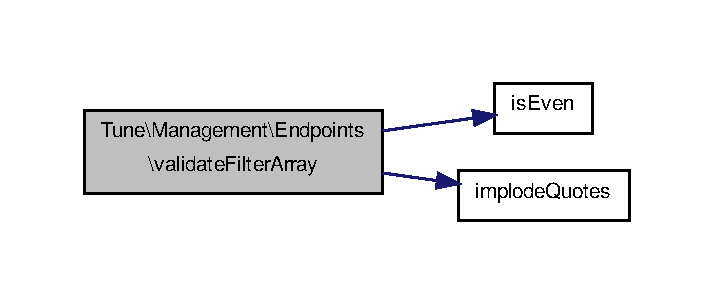
\includegraphics[width=342pt]{namespaceTune_1_1Management_1_1Endpoints_ae2d0d6742ce18cb5d94c1e0fb5ebdabe_cgraph}
\end{center}
\end{figure}




Here is the caller graph for this function\-:
\nopagebreak
\begin{figure}[H]
\begin{center}
\leavevmode
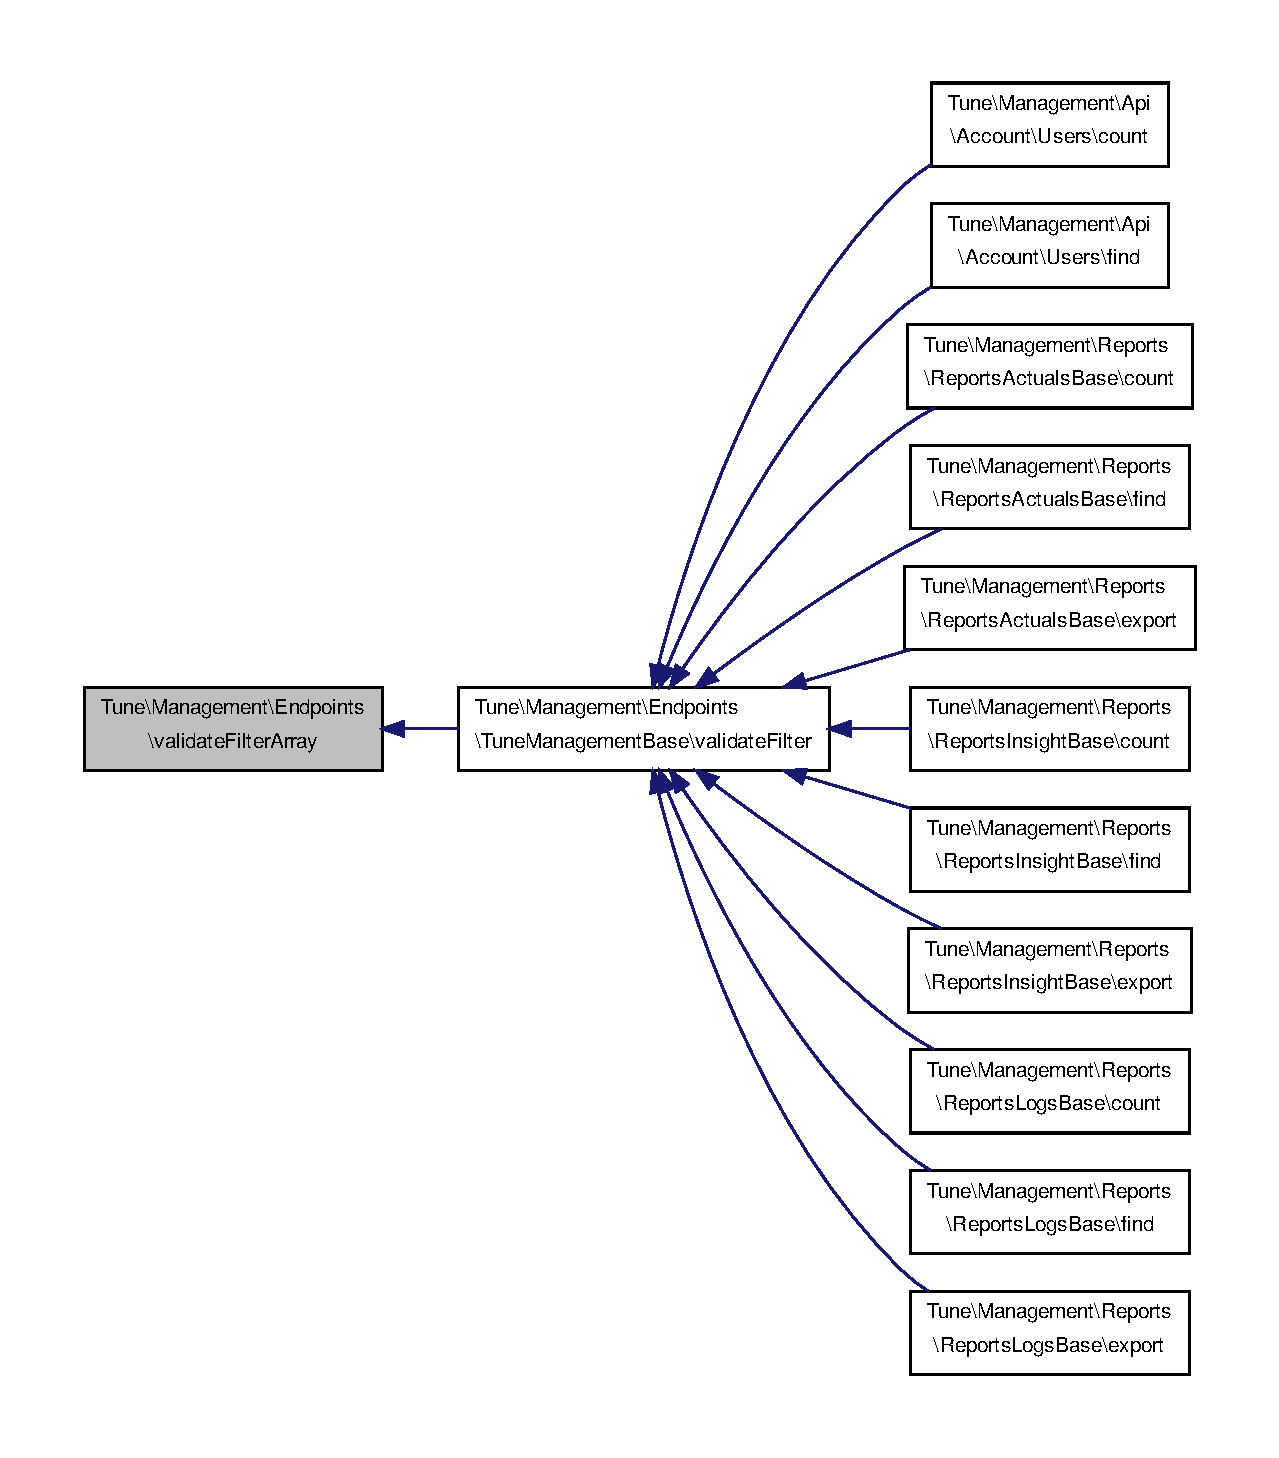
\includegraphics[width=350pt]{namespaceTune_1_1Management_1_1Endpoints_ae2d0d6742ce18cb5d94c1e0fb5ebdabe_icgraph}
\end{center}
\end{figure}


\hypertarget{namespaceTune_1_1Management_1_1Endpoints_a8a3f8f7bc986da92a05b19f9ca804e2d}{\index{Tune\-::\-Management\-::\-Endpoints@{Tune\-::\-Management\-::\-Endpoints}!validate\-Filter\-String@{validate\-Filter\-String}}
\index{validate\-Filter\-String@{validate\-Filter\-String}!Tune::Management::Endpoints@{Tune\-::\-Management\-::\-Endpoints}}
\subsubsection[{validate\-Filter\-String}]{\setlength{\rightskip}{0pt plus 5cm}Tune\textbackslash{}\-Management\textbackslash{}\-Endpoints\textbackslash{}validate\-Filter\-String (
\begin{DoxyParamCaption}
\item[{}]{\$fields, }
\item[{}]{\$filter\-\_\-operations, }
\item[{}]{\$filter\-\_\-conjunctions, }
\item[{}]{\$filter}
\end{DoxyParamCaption}
)}}\label{namespaceTune_1_1Management_1_1Endpoints_a8a3f8f7bc986da92a05b19f9ca804e2d}


Validate provided filter string is properly formatted query. 


\begin{DoxyParams}[1]{Parameters}
array & {\em \$fields} & \\
\hline
array & {\em \$filter\-\_\-operations} & \\
\hline
array & {\em \$filter\-\_\-conjunctions} & \\
\hline
string & {\em \$filter} & \\
\hline
\end{DoxyParams}
\begin{DoxyReturn}{Returns}
array 
\end{DoxyReturn}

\begin{DoxyExceptions}{Exceptions}
{\em \textbackslash{}\-Tune\textbackslash{}\-Common\textbackslash{}\-Tune\-Sdk\-Exception} & \\
\hline
\end{DoxyExceptions}


Definition at line 579 of file Tune\-Management\-Base.\-php.


\begin{DoxyCode}
580 \{
581     $filter\_expr = array();
582 
583     \textcolor{keywordflow}{if} (!is\_string($filter)) \{
584         \textcolor{keywordflow}{throw} \textcolor{keyword}{new} TuneSdkException(\textcolor{stringliteral}{"Parameter 'filter' expects string."});
585     \}
586 
587     $pp = \textcolor{keyword}{new} ParenthesesParser();
588 
589     $filter\_parts = $pp->parse($filter);
590 
591     \textcolor{keywordflow}{foreach} ($filter\_parts as $key => $filter\_part) \{
592         \textcolor{keywordflow}{if} (is\_string($filter\_part)) \{
593 
594             $filter\_conjunction = trim($filter\_part);
595             \textcolor{keywordflow}{if} (\hyperlink{Helper_8php_ab83bcc4e2fd231ef49158704ecaa2480}{isEven}($key)) \{
596                 \textcolor{keywordflow}{throw} \textcolor{keyword}{new} TuneSdkException(\textcolor{stringliteral}{"Invalid placement of conjunction in filter parameter: '\{$key\}'.
      "});
597             \}
598             \textcolor{keywordflow}{if} (!in\_array($filter\_conjunction, $filter\_conjunctions)) \{
599                 \textcolor{keywordflow}{throw} \textcolor{keyword}{new} TuneSdkException(\textcolor{stringliteral}{"Invalid conjunction in filter parameter:
       '\{$filter\_conjunction\}'."});
600             \}
601 
602             $filter\_expr[] = $filter\_conjunction;
603         \} elseif (is\_array($filter\_part)) \{
604             $sub\_expr\_part = $filter\_part[0];
605             $sub\_filter\_expr\_parts = explode(\textcolor{stringliteral}{" "}, $sub\_expr\_part);
606 
607             $field = array\_shift($sub\_filter\_expr\_parts);
608             \textcolor{keywordflow}{if} (!is\_null($fields) && is\_array($fields) && !in\_array($field, $fields)) \{
609                 \textcolor{keywordflow}{throw} \textcolor{keyword}{new} TuneSdkException(\textcolor{stringliteral}{"Invalid field in filter parameter: '\{$field\}'."});
610             \}
611             $sub\_filter\_expr\_part\_end = trim(end($sub\_filter\_expr\_parts));
612             $sub\_filter\_expr\_part\_end\_no\_quotes = trim($sub\_filter\_expr\_part\_end, \textcolor{stringliteral}{"'"});
613 
614             $sub\_filter\_expr\_value = null;
615             \textcolor{keywordflow}{if} ($sub\_filter\_expr\_part\_end\_no\_quotes != $sub\_filter\_expr\_part\_end) \{
616                 $sub\_filter\_expr\_value = array\_pop($sub\_filter\_expr\_parts);
617             \}
618             $sub\_filter\_expr\_operator = implode(\textcolor{stringliteral}{" "}, $sub\_filter\_expr\_parts);
619             $sub\_filter\_expr\_operator = trim($sub\_filter\_expr\_operator);
620             \textcolor{keywordflow}{if} (!in\_array($sub\_filter\_expr\_operator, $filter\_operations)) \{
621                 \textcolor{keywordflow}{throw} \textcolor{keyword}{new} TuneSdkException(\textcolor{stringliteral}{"Invalid operator in filter parameter '\{$filter\}':
       '\{$sub\_filter\_expr\_operator\}'."});
622             \}
623 
624             \textcolor{keywordflow}{if} (count($filter\_part) == 2) \{
625                 $sub\_filter\_expr\_value =  $filter\_part[1];
626             \}
627 
628             $sub\_filter = array (
629                 \textcolor{stringliteral}{"column"} => $field,
630                 \textcolor{stringliteral}{"operator"} => $sub\_filter\_expr\_operator
631             );
632 
633             \textcolor{keywordflow}{if} ($sub\_filter\_expr\_value) \{
634                 $sub\_filter[\textcolor{stringliteral}{"value"}] = $sub\_filter\_expr\_part\_end;
635             \}
636 
637             $filter\_expr[] = $sub\_filter;
638         \}
639     \}
640 
641     \textcolor{keywordflow}{return} $filter\_expr;
642 \}
\end{DoxyCode}


Here is the call graph for this function\-:
\nopagebreak
\begin{figure}[H]
\begin{center}
\leavevmode
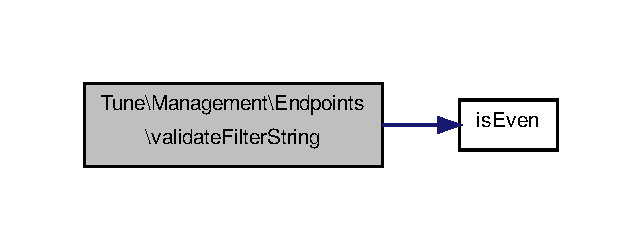
\includegraphics[width=308pt]{namespaceTune_1_1Management_1_1Endpoints_a8a3f8f7bc986da92a05b19f9ca804e2d_cgraph}
\end{center}
\end{figure}




Here is the caller graph for this function\-:
\nopagebreak
\begin{figure}[H]
\begin{center}
\leavevmode
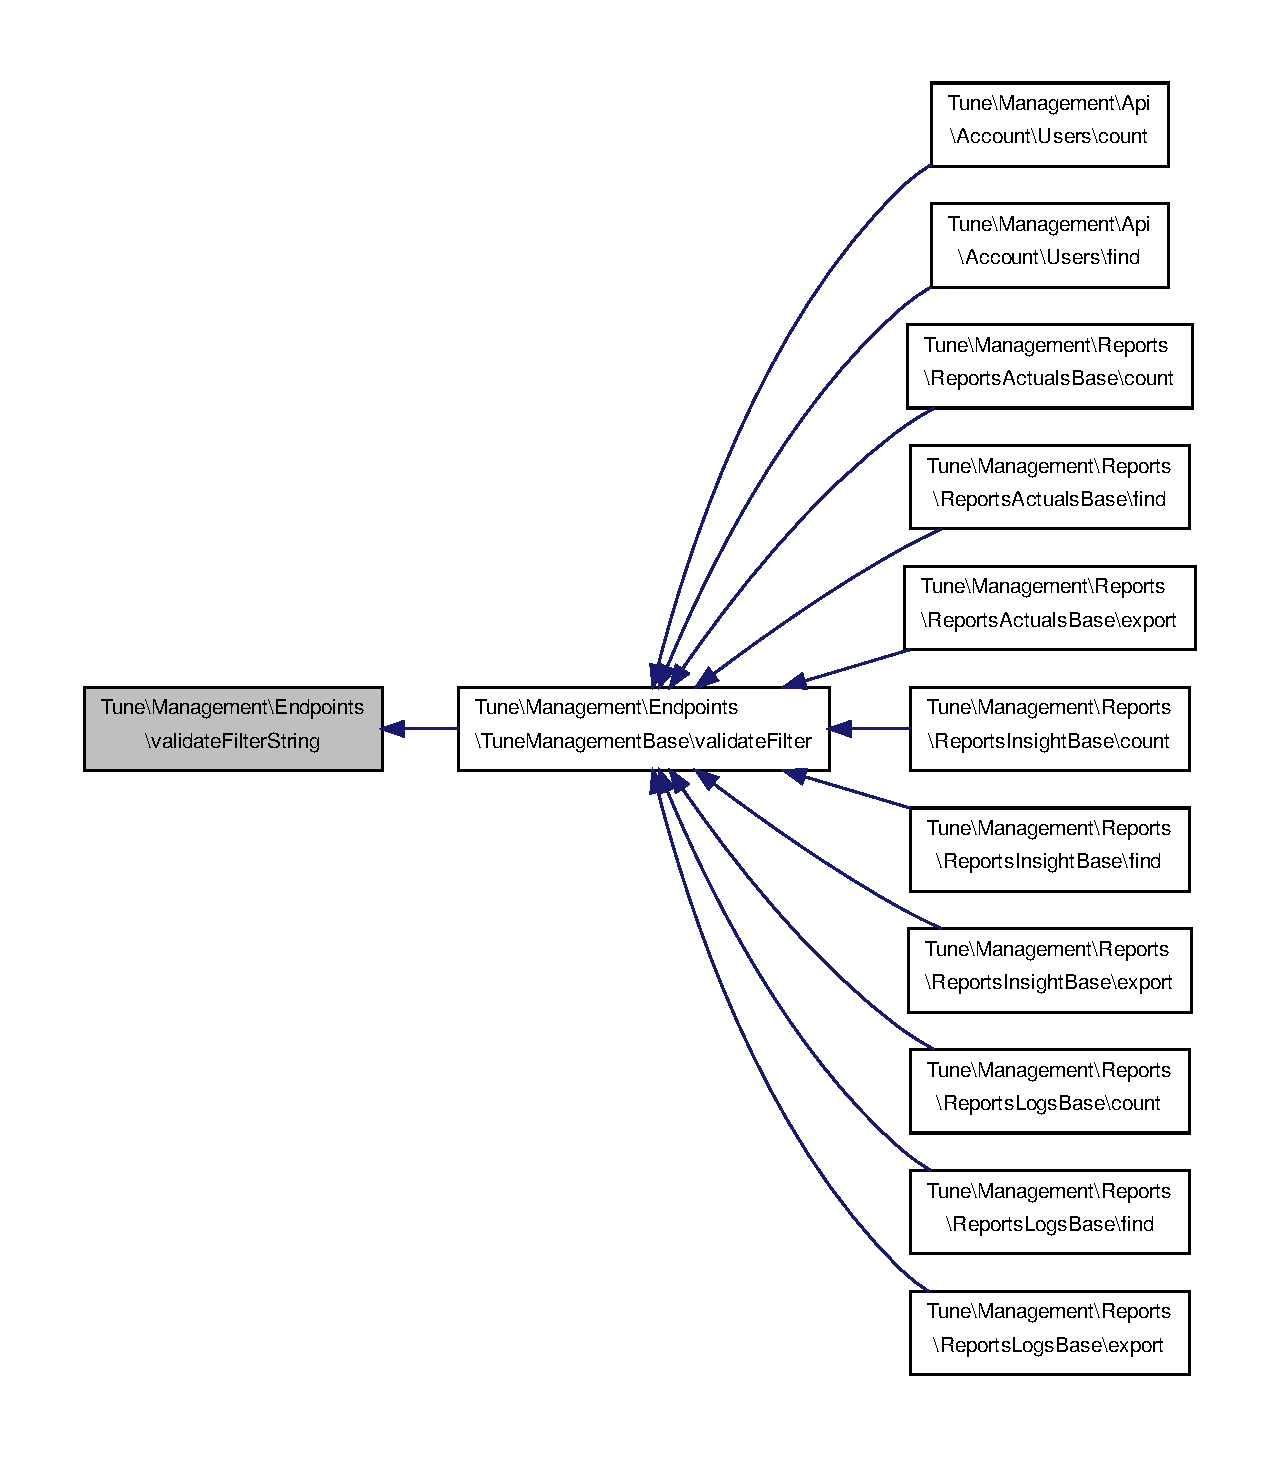
\includegraphics[width=350pt]{namespaceTune_1_1Management_1_1Endpoints_a8a3f8f7bc986da92a05b19f9ca804e2d_icgraph}
\end{center}
\end{figure}



\hypertarget{namespaceTune_1_1Management_1_1Reports}{\section{Tune\textbackslash{}Management\textbackslash{}Reports Namespace Reference}
\label{namespaceTune_1_1Management_1_1Reports}\index{Tune\textbackslash{}\-Management\textbackslash{}\-Reports@{Tune\textbackslash{}\-Management\textbackslash{}\-Reports}}
}
\subsection*{Data Structures}
\begin{DoxyCompactItemize}
\item 
class \hyperlink{classTune_1_1Management_1_1Reports_1_1ReportExportWorker}{Report\-Export\-Worker}
\item 
class \hyperlink{classTune_1_1Management_1_1Reports_1_1ReportReaderBase}{Report\-Reader\-Base}
\item 
class \hyperlink{classTune_1_1Management_1_1Reports_1_1ReportReaderCSV}{Report\-Reader\-C\-S\-V}
\item 
class \hyperlink{classTune_1_1Management_1_1Reports_1_1ReportReaderJSON}{Report\-Reader\-J\-S\-O\-N}
\item 
class \hyperlink{classTune_1_1Management_1_1Reports_1_1ReportsActualsBase}{Reports\-Actuals\-Base}
\item 
class \hyperlink{classTune_1_1Management_1_1Reports_1_1ReportsBase}{Reports\-Base}
\item 
class \hyperlink{classTune_1_1Management_1_1Reports_1_1ReportsInsightBase}{Reports\-Insight\-Base}
\item 
class \hyperlink{classTune_1_1Management_1_1Reports_1_1ReportsLogsBase}{Reports\-Logs\-Base}
\end{DoxyCompactItemize}

\hypertarget{namespaceTune_1_1Management_1_1Service}{\section{Tune\textbackslash{}Management\textbackslash{}Service Namespace Reference}
\label{namespaceTune_1_1Management_1_1Service}\index{Tune\textbackslash{}\-Management\textbackslash{}\-Service@{Tune\textbackslash{}\-Management\textbackslash{}\-Service}}
}
\subsection*{Data Structures}
\begin{DoxyCompactItemize}
\item 
class \hyperlink{classTune_1_1Management_1_1Service_1_1Proxy}{Proxy}
\item 
class \hyperlink{classTune_1_1Management_1_1Service_1_1QueryStringBuilder}{Query\-String\-Builder}
\item 
class \hyperlink{classTune_1_1Management_1_1Service_1_1Request}{Request}
\item 
class \hyperlink{classTune_1_1Management_1_1Service_1_1Response}{Response}
\item 
class \hyperlink{classTune_1_1Management_1_1Service_1_1TuneManagementClient}{Tune\-Management\-Client}
\end{DoxyCompactItemize}
\subsection*{Variables}
\begin{DoxyCompactItemize}
\item 
const \hyperlink{namespaceTune_1_1Management_1_1Service_a7bce96e6c1888a8f3b18a9802d6a2ced}{T\-U\-N\-E\-\_\-\-M\-A\-N\-A\-G\-E\-M\-E\-N\-T\-\_\-\-A\-P\-I\-\_\-\-B\-A\-S\-E\-\_\-\-U\-R\-L} \char`\"{}https\-://api.\-mobileapptracking.\-com\char`\"{}
\item 
const \hyperlink{namespaceTune_1_1Management_1_1Service_a4a4f959118a3c1ce5c479805610f9036}{T\-U\-N\-E\-\_\-\-M\-A\-N\-A\-G\-E\-M\-E\-N\-T\-\_\-\-A\-P\-I\-\_\-\-V\-E\-R\-S\-I\-O\-N} \char`\"{}v2\char`\"{}
\end{DoxyCompactItemize}


\subsection{Variable Documentation}
\hypertarget{namespaceTune_1_1Management_1_1Service_a7bce96e6c1888a8f3b18a9802d6a2ced}{\index{Tune\-::\-Management\-::\-Service@{Tune\-::\-Management\-::\-Service}!T\-U\-N\-E\-\_\-\-M\-A\-N\-A\-G\-E\-M\-E\-N\-T\-\_\-\-A\-P\-I\-\_\-\-B\-A\-S\-E\-\_\-\-U\-R\-L@{T\-U\-N\-E\-\_\-\-M\-A\-N\-A\-G\-E\-M\-E\-N\-T\-\_\-\-A\-P\-I\-\_\-\-B\-A\-S\-E\-\_\-\-U\-R\-L}}
\index{T\-U\-N\-E\-\_\-\-M\-A\-N\-A\-G\-E\-M\-E\-N\-T\-\_\-\-A\-P\-I\-\_\-\-B\-A\-S\-E\-\_\-\-U\-R\-L@{T\-U\-N\-E\-\_\-\-M\-A\-N\-A\-G\-E\-M\-E\-N\-T\-\_\-\-A\-P\-I\-\_\-\-B\-A\-S\-E\-\_\-\-U\-R\-L}!Tune::Management::Service@{Tune\-::\-Management\-::\-Service}}
\subsubsection[{T\-U\-N\-E\-\_\-\-M\-A\-N\-A\-G\-E\-M\-E\-N\-T\-\_\-\-A\-P\-I\-\_\-\-B\-A\-S\-E\-\_\-\-U\-R\-L}]{\setlength{\rightskip}{0pt plus 5cm}const Tune\-::\-Management\-::\-Service\textbackslash{}\-T\-U\-N\-E\-\_\-\-M\-A\-N\-A\-G\-E\-M\-E\-N\-T\-\_\-\-A\-P\-I\-\_\-\-B\-A\-S\-E\-\_\-\-U\-R\-L \char`\"{}https\-://api.\-mobileapptracking.\-com\char`\"{}}}\label{namespaceTune_1_1Management_1_1Service_a7bce96e6c1888a8f3b18a9802d6a2ced}


Definition at line 40 of file Constants.\-php.

\hypertarget{namespaceTune_1_1Management_1_1Service_a4a4f959118a3c1ce5c479805610f9036}{\index{Tune\-::\-Management\-::\-Service@{Tune\-::\-Management\-::\-Service}!T\-U\-N\-E\-\_\-\-M\-A\-N\-A\-G\-E\-M\-E\-N\-T\-\_\-\-A\-P\-I\-\_\-\-V\-E\-R\-S\-I\-O\-N@{T\-U\-N\-E\-\_\-\-M\-A\-N\-A\-G\-E\-M\-E\-N\-T\-\_\-\-A\-P\-I\-\_\-\-V\-E\-R\-S\-I\-O\-N}}
\index{T\-U\-N\-E\-\_\-\-M\-A\-N\-A\-G\-E\-M\-E\-N\-T\-\_\-\-A\-P\-I\-\_\-\-V\-E\-R\-S\-I\-O\-N@{T\-U\-N\-E\-\_\-\-M\-A\-N\-A\-G\-E\-M\-E\-N\-T\-\_\-\-A\-P\-I\-\_\-\-V\-E\-R\-S\-I\-O\-N}!Tune::Management::Service@{Tune\-::\-Management\-::\-Service}}
\subsubsection[{T\-U\-N\-E\-\_\-\-M\-A\-N\-A\-G\-E\-M\-E\-N\-T\-\_\-\-A\-P\-I\-\_\-\-V\-E\-R\-S\-I\-O\-N}]{\setlength{\rightskip}{0pt plus 5cm}const Tune\-::\-Management\-::\-Service\textbackslash{}\-T\-U\-N\-E\-\_\-\-M\-A\-N\-A\-G\-E\-M\-E\-N\-T\-\_\-\-A\-P\-I\-\_\-\-V\-E\-R\-S\-I\-O\-N \char`\"{}v2\char`\"{}}}\label{namespaceTune_1_1Management_1_1Service_a4a4f959118a3c1ce5c479805610f9036}


Definition at line 41 of file Constants.\-php.


\hypertarget{namespaceTune__PHP__SDK}{\section{Tune\-\_\-\-P\-H\-P\-\_\-\-S\-D\-K Namespace Reference}
\label{namespaceTune__PHP__SDK}\index{Tune\-\_\-\-P\-H\-P\-\_\-\-S\-D\-K@{Tune\-\_\-\-P\-H\-P\-\_\-\-S\-D\-K}}
}


Tune\-Service\-Exception is thrown when the \hyperlink{namespaceTune}{Tune} Mobile\-App\-Tracking Management A\-P\-I return a Failure Tune\-Response for a given Tune\-Request.  




\subsection{Detailed Description}
Tune\-Service\-Exception is thrown when the \hyperlink{namespaceTune}{Tune} Mobile\-App\-Tracking Management A\-P\-I return a Failure Tune\-Response for a given Tune\-Request. The successful response to request.

Request provides the basic interface for all the possible request types.

Query\-String\-Builder incrementally builds query string element by element.

\begin{DoxyAuthor}{Author}
Jeff Tanner \href{mailto:jefft@tune.com}{\tt jefft@tune.\-com} 
\end{DoxyAuthor}
\begin{DoxyCopyright}{Copyright}
2014 \hyperlink{namespaceTune}{Tune} (\href{http://www.tune.com}{\tt http\-://www.\-tune.\-com})  \href{http://opensource.org/licenses/MIT}{\tt http\-://opensource.\-org/licenses/\-M\-I\-T} The M\-I\-T License (M\-I\-T) 
\end{DoxyCopyright}
\begin{DoxyVersion}{Version}
0.\-9.\-1 \hyperlink{}{Tune Developer Community }
\end{DoxyVersion}
public 
\chapter{Data Structure Documentation}
\hypertarget{classTune_1_1Management_1_1Api_1_1Account}{\section{Tune\textbackslash{}Management\textbackslash{}Api\textbackslash{}Account Class Reference}
\label{classTune_1_1Management_1_1Api_1_1Account}\index{Tune\textbackslash{}\-Management\textbackslash{}\-Api\textbackslash{}\-Account@{Tune\textbackslash{}\-Management\textbackslash{}\-Api\textbackslash{}\-Account}}
}


Inheritance diagram for Tune\textbackslash{}Management\textbackslash{}Api\textbackslash{}Account\-:
\nopagebreak
\begin{figure}[H]
\begin{center}
\leavevmode
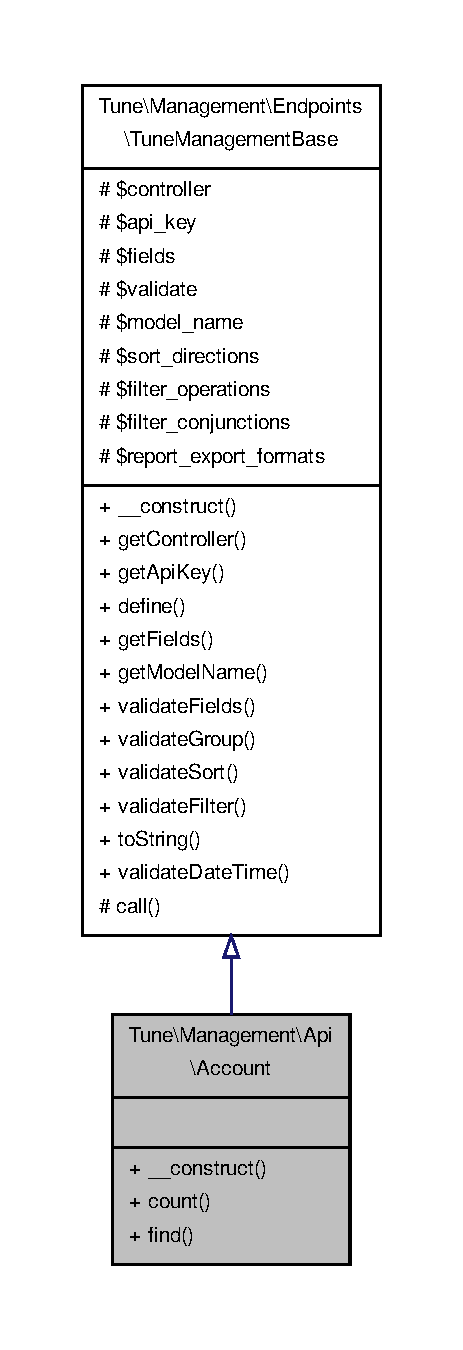
\includegraphics[height=550pt]{classTune_1_1Management_1_1Api_1_1Account__inherit__graph}
\end{center}
\end{figure}


Collaboration diagram for Tune\textbackslash{}Management\textbackslash{}Api\textbackslash{}Account\-:
\nopagebreak
\begin{figure}[H]
\begin{center}
\leavevmode
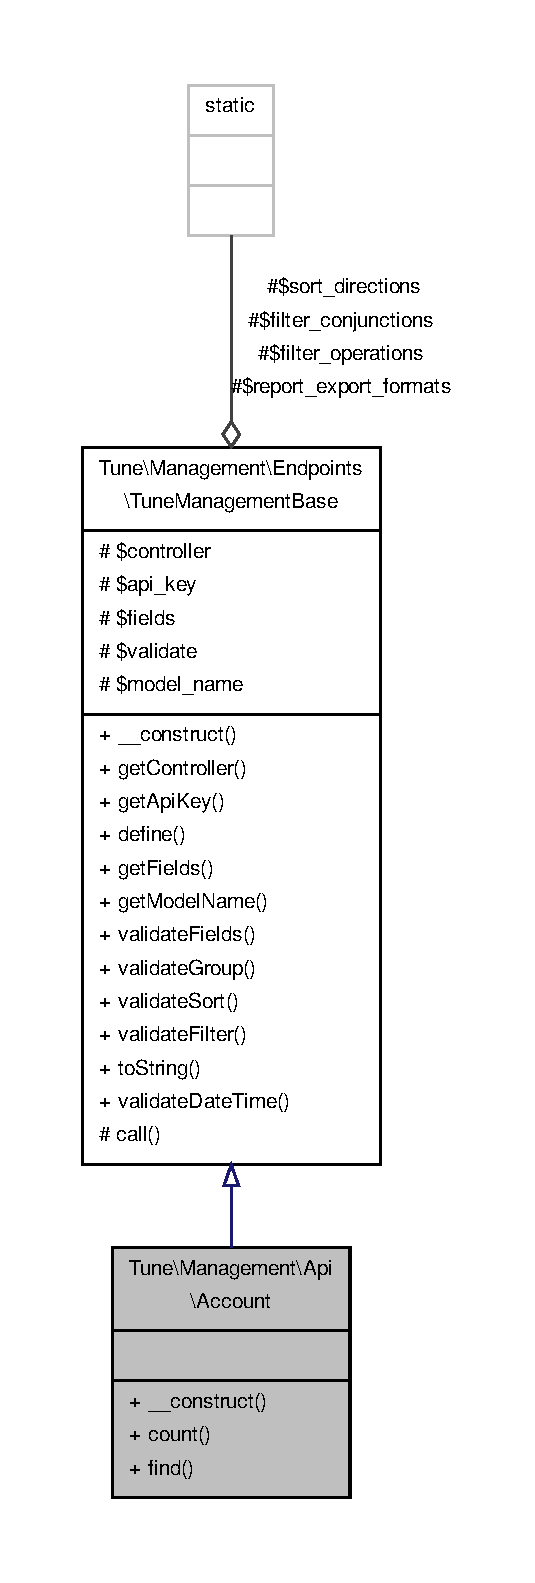
\includegraphics[height=550pt]{classTune_1_1Management_1_1Api_1_1Account__coll__graph}
\end{center}
\end{figure}
\subsection*{Public Member Functions}
\begin{DoxyCompactItemize}
\item 
\hyperlink{classTune_1_1Management_1_1Api_1_1Account_a5b8e619064ca9ae86956159732167d6e}{\-\_\-\-\_\-construct} (\$api\-\_\-key, \$validate=false)
\begin{DoxyCompactList}\small\item\em Constructor. \end{DoxyCompactList}\item 
\hyperlink{classTune_1_1Management_1_1Api_1_1Account_aa5c03dc594104c4d20116147a8679b34}{count} (\$filter=null)
\begin{DoxyCompactList}\small\item\em Counts all existing records that match filter criteria and returns an array of found model data. \end{DoxyCompactList}\item 
\hyperlink{classTune_1_1Management_1_1Api_1_1Account_a84ed9a047288703eddfbde9d94348ccb}{find} (\$fields=null, \$filter=null, \$limit=null, \$page=null, \$sort=null)
\begin{DoxyCompactList}\small\item\em Finds all existing records that match filter criteria and returns an array of found model data. \end{DoxyCompactList}\end{DoxyCompactItemize}
\subsection*{Additional Inherited Members}


\subsection{Detailed Description}


Definition at line 46 of file Account.\-php.



\subsection{Constructor \& Destructor Documentation}
\hypertarget{classTune_1_1Management_1_1Api_1_1Account_a5b8e619064ca9ae86956159732167d6e}{\index{Tune\-::\-Management\-::\-Api\-::\-Account@{Tune\-::\-Management\-::\-Api\-::\-Account}!\-\_\-\-\_\-construct@{\-\_\-\-\_\-construct}}
\index{\-\_\-\-\_\-construct@{\-\_\-\-\_\-construct}!Tune::Management::Api::Account@{Tune\-::\-Management\-::\-Api\-::\-Account}}
\subsubsection[{\-\_\-\-\_\-construct}]{\setlength{\rightskip}{0pt plus 5cm}Tune\textbackslash{}\-Management\textbackslash{}\-Api\textbackslash{}\-Account\-::\-\_\-\-\_\-construct (
\begin{DoxyParamCaption}
\item[{}]{\$api\-\_\-key, }
\item[{}]{\$validate = {\ttfamily false}}
\end{DoxyParamCaption}
)}}\label{classTune_1_1Management_1_1Api_1_1Account_a5b8e619064ca9ae86956159732167d6e}


Constructor. 


\begin{DoxyParams}[1]{Parameters}
string & {\em \$api\-\_\-key} & Mobile\-App\-Tracking A\-P\-I Key \\
\hline
bool & {\em \$validate} & Validate fields used by actions' parameters. \\
\hline
\end{DoxyParams}


Definition at line 54 of file Account.\-php.


\begin{DoxyCode}
57       \{
58         parent::\_\_contruct(
59             \textcolor{stringliteral}{"account"},
60             \hyperlink{classTune_1_1Management_1_1Endpoints_1_1TuneManagementBase_ac53649b4bc72055e1d55e53e0b6f244e}{$api\_key},
61             \hyperlink{classTune_1_1Management_1_1Endpoints_1_1TuneManagementBase_a264eed27b0a1c963808fc7eab6da98bc}{$validate}
62         );
63     \}
\end{DoxyCode}


\subsection{Member Function Documentation}
\hypertarget{classTune_1_1Management_1_1Api_1_1Account_aa5c03dc594104c4d20116147a8679b34}{\index{Tune\-::\-Management\-::\-Api\-::\-Account@{Tune\-::\-Management\-::\-Api\-::\-Account}!count@{count}}
\index{count@{count}!Tune::Management::Api::Account@{Tune\-::\-Management\-::\-Api\-::\-Account}}
\subsubsection[{count}]{\setlength{\rightskip}{0pt plus 5cm}Tune\textbackslash{}\-Management\textbackslash{}\-Api\textbackslash{}\-Account\-::count (
\begin{DoxyParamCaption}
\item[{}]{\$filter = {\ttfamily null}}
\end{DoxyParamCaption}
)}}\label{classTune_1_1Management_1_1Api_1_1Account_aa5c03dc594104c4d20116147a8679b34}


Counts all existing records that match filter criteria and returns an array of found model data. 


\begin{DoxyParams}[1]{Parameters}
string & {\em \$filter} & Filter the results and apply conditions that must be met for records to be included in data.\\
\hline
\end{DoxyParams}
\begin{DoxyReturn}{Returns}
object 
\end{DoxyReturn}


Definition at line 75 of file Account.\-php.


\begin{DoxyCode}
77       \{
78         $query\_string\_dict = [];
79         $query\_string\_dict[\textcolor{stringliteral}{'filter'}] = $filter;
80 
81         \textcolor{keywordflow}{return} parent::call(
82             \textcolor{stringliteral}{"count"},
83             $query\_string\_dict
84         );
85     \}
\end{DoxyCode}
\hypertarget{classTune_1_1Management_1_1Api_1_1Account_a84ed9a047288703eddfbde9d94348ccb}{\index{Tune\-::\-Management\-::\-Api\-::\-Account@{Tune\-::\-Management\-::\-Api\-::\-Account}!find@{find}}
\index{find@{find}!Tune::Management::Api::Account@{Tune\-::\-Management\-::\-Api\-::\-Account}}
\subsubsection[{find}]{\setlength{\rightskip}{0pt plus 5cm}Tune\textbackslash{}\-Management\textbackslash{}\-Api\textbackslash{}\-Account\-::find (
\begin{DoxyParamCaption}
\item[{}]{\$fields = {\ttfamily null}, }
\item[{}]{\$filter = {\ttfamily null}, }
\item[{}]{\$limit = {\ttfamily null}, }
\item[{}]{\$page = {\ttfamily null}, }
\item[{}]{\$sort = {\ttfamily null}}
\end{DoxyParamCaption}
)}}\label{classTune_1_1Management_1_1Api_1_1Account_a84ed9a047288703eddfbde9d94348ccb}


Finds all existing records that match filter criteria and returns an array of found model data. 


\begin{DoxyParams}[1]{Parameters}
string & {\em \$filter} & Filter the results and apply conditions that must be met for records to be included in data. \\
\hline
string & {\em \$fields} & No value returns default fields, \char`\"{}$\ast$\char`\"{} returns all available fields, or provide specific fields. \\
\hline
int & {\em \$limit} & Limit number of results, default 10, 0 shows all. \\
\hline
int & {\em \$page} & Pagination, default 1. \\
\hline
dict & {\em \$sort} & Expression defining sorting found records in result set base upon provided fields and its modifier (A\-S\-C or D\-E\-S\-C).\\
\hline
\end{DoxyParams}
\begin{DoxyReturn}{Returns}
object 
\end{DoxyReturn}


Definition at line 106 of file Account.\-php.


\begin{DoxyCode}
112       \{
113         $query\_string\_dict = [];
114         $query\_string\_dict[\textcolor{stringliteral}{'fields'}] = \hyperlink{classTune_1_1Management_1_1Endpoints_1_1TuneManagementBase_a215be5184c46eee7b2b3febaba85f91b}{$fields};
115         $query\_string\_dict[\textcolor{stringliteral}{'filter'}] = $filter;
116         $query\_string\_dict[\textcolor{stringliteral}{'limit'}] = $limit;
117         $query\_string\_dict[\textcolor{stringliteral}{'page'}] = $page;
118         $query\_string\_dict[\textcolor{stringliteral}{'sort'}] = $sort;
119 
120         \textcolor{keywordflow}{return} parent::call(
121             \textcolor{stringliteral}{"find"},
122             $query\_string\_dict
123         );
124     \}
\end{DoxyCode}


The documentation for this class was generated from the following file\-:\begin{DoxyCompactItemize}
\item 
lib/\-Tune/\-Management/\-Api/\hyperlink{Account_8php}{Account.\-php}\end{DoxyCompactItemize}

\hypertarget{classTune_1_1Management_1_1Api_1_1Advertiser}{\section{Tune\textbackslash{}Management\textbackslash{}Api\textbackslash{}Advertiser Class Reference}
\label{classTune_1_1Management_1_1Api_1_1Advertiser}\index{Tune\textbackslash{}\-Management\textbackslash{}\-Api\textbackslash{}\-Advertiser@{Tune\textbackslash{}\-Management\textbackslash{}\-Api\textbackslash{}\-Advertiser}}
}


Inheritance diagram for Tune\textbackslash{}Management\textbackslash{}Api\textbackslash{}Advertiser\-:
\nopagebreak
\begin{figure}[H]
\begin{center}
\leavevmode
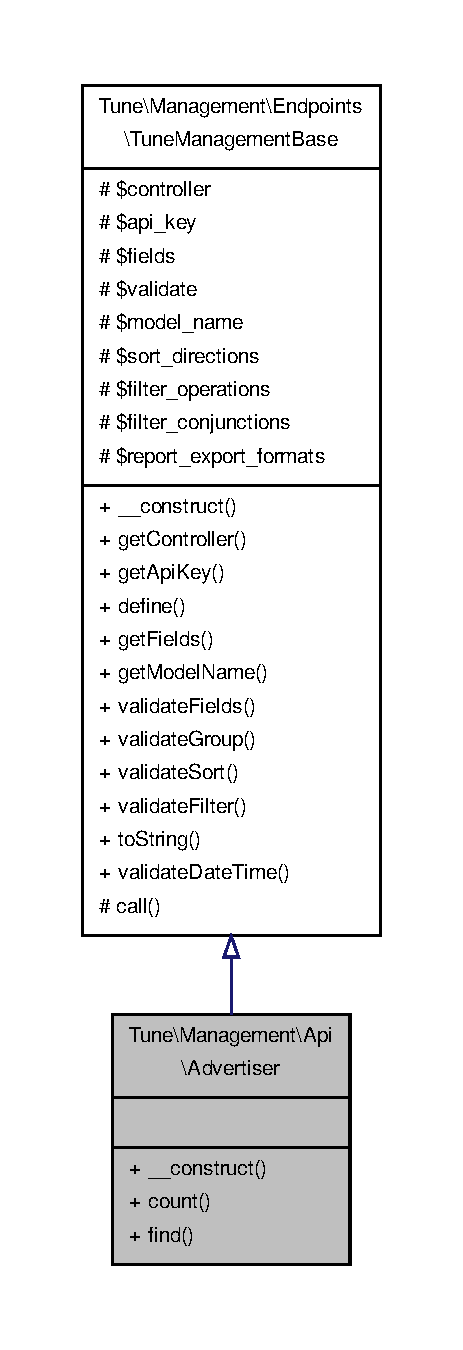
\includegraphics[height=550pt]{classTune_1_1Management_1_1Api_1_1Advertiser__inherit__graph}
\end{center}
\end{figure}


Collaboration diagram for Tune\textbackslash{}Management\textbackslash{}Api\textbackslash{}Advertiser\-:
\nopagebreak
\begin{figure}[H]
\begin{center}
\leavevmode
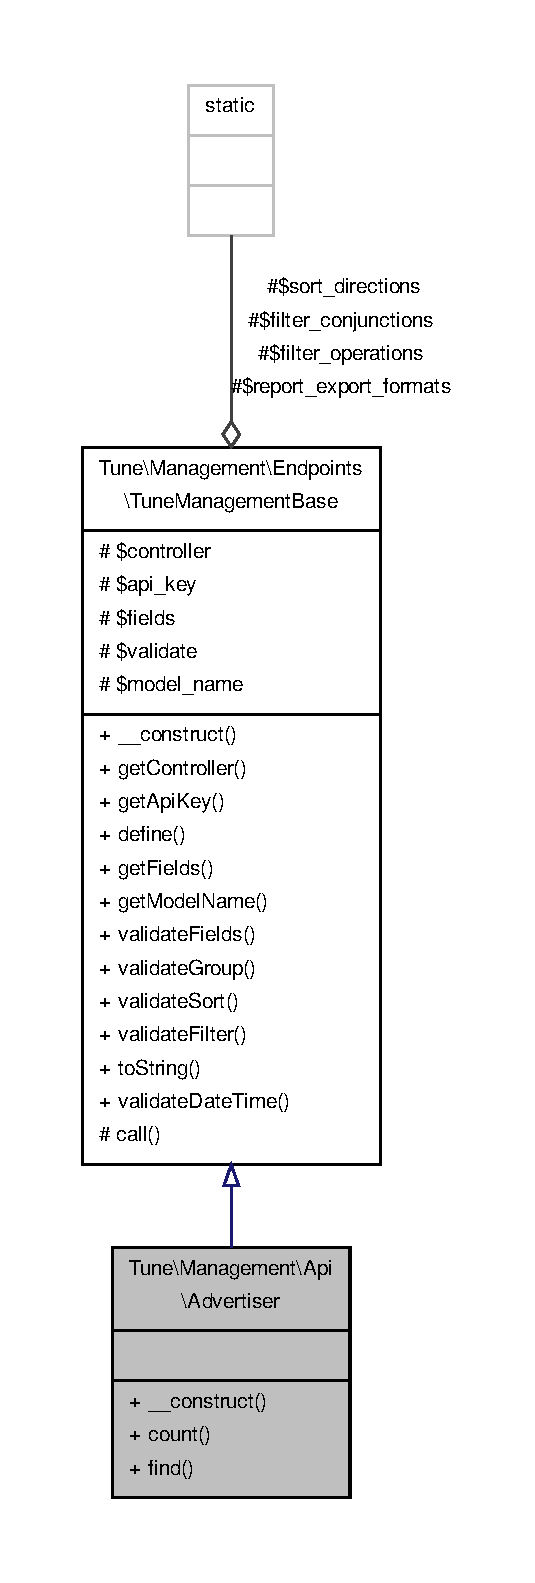
\includegraphics[height=550pt]{classTune_1_1Management_1_1Api_1_1Advertiser__coll__graph}
\end{center}
\end{figure}
\subsection*{Public Member Functions}
\begin{DoxyCompactItemize}
\item 
\hyperlink{classTune_1_1Management_1_1Api_1_1Advertiser_ad29063af36a66b7041962c4aa8002d3b}{\-\_\-\-\_\-construct} (\$api\-\_\-key, \$validate=false)
\begin{DoxyCompactList}\small\item\em Constructor. \end{DoxyCompactList}\item 
\hyperlink{classTune_1_1Management_1_1Api_1_1Advertiser_a8b88dd2b30650e6701e132b6074cbc30}{count} (\$filter=null)
\begin{DoxyCompactList}\small\item\em Counts all existing records that match filter criteria and returns an array of found model data. \end{DoxyCompactList}\item 
\hyperlink{classTune_1_1Management_1_1Api_1_1Advertiser_a5349eab046c6cc4f801f1a00dd7068a9}{find} (\$fields=null, \$filter=null, \$limit=null, \$page=null, \$sort=null)
\begin{DoxyCompactList}\small\item\em Finds all existing records that match filter criteria and returns an array of found model data. \end{DoxyCompactList}\end{DoxyCompactItemize}
\subsection*{Additional Inherited Members}


\subsection{Detailed Description}


Definition at line 46 of file Advertiser.\-php.



\subsection{Constructor \& Destructor Documentation}
\hypertarget{classTune_1_1Management_1_1Api_1_1Advertiser_ad29063af36a66b7041962c4aa8002d3b}{\index{Tune\-::\-Management\-::\-Api\-::\-Advertiser@{Tune\-::\-Management\-::\-Api\-::\-Advertiser}!\-\_\-\-\_\-construct@{\-\_\-\-\_\-construct}}
\index{\-\_\-\-\_\-construct@{\-\_\-\-\_\-construct}!Tune::Management::Api::Advertiser@{Tune\-::\-Management\-::\-Api\-::\-Advertiser}}
\subsubsection[{\-\_\-\-\_\-construct}]{\setlength{\rightskip}{0pt plus 5cm}Tune\textbackslash{}\-Management\textbackslash{}\-Api\textbackslash{}\-Advertiser\-::\-\_\-\-\_\-construct (
\begin{DoxyParamCaption}
\item[{}]{\$api\-\_\-key, }
\item[{}]{\$validate = {\ttfamily false}}
\end{DoxyParamCaption}
)}}\label{classTune_1_1Management_1_1Api_1_1Advertiser_ad29063af36a66b7041962c4aa8002d3b}


Constructor. 


\begin{DoxyParams}[1]{Parameters}
string & {\em \$api\-\_\-key} & Mobile\-App\-Tracking A\-P\-I Key \\
\hline
bool & {\em \$validate} & Validate fields used by actions' parameters. \\
\hline
\end{DoxyParams}


Definition at line 54 of file Advertiser.\-php.


\begin{DoxyCode}
57       \{
58         parent::\_\_contruct(
59             \textcolor{stringliteral}{"advertiser"},
60             \hyperlink{classTune_1_1Management_1_1Endpoints_1_1TuneManagementBase_ac53649b4bc72055e1d55e53e0b6f244e}{$api\_key},
61             \hyperlink{classTune_1_1Management_1_1Endpoints_1_1TuneManagementBase_a264eed27b0a1c963808fc7eab6da98bc}{$validate}
62         );
63     \}
\end{DoxyCode}


\subsection{Member Function Documentation}
\hypertarget{classTune_1_1Management_1_1Api_1_1Advertiser_a8b88dd2b30650e6701e132b6074cbc30}{\index{Tune\-::\-Management\-::\-Api\-::\-Advertiser@{Tune\-::\-Management\-::\-Api\-::\-Advertiser}!count@{count}}
\index{count@{count}!Tune::Management::Api::Advertiser@{Tune\-::\-Management\-::\-Api\-::\-Advertiser}}
\subsubsection[{count}]{\setlength{\rightskip}{0pt plus 5cm}Tune\textbackslash{}\-Management\textbackslash{}\-Api\textbackslash{}\-Advertiser\-::count (
\begin{DoxyParamCaption}
\item[{}]{\$filter = {\ttfamily null}}
\end{DoxyParamCaption}
)}}\label{classTune_1_1Management_1_1Api_1_1Advertiser_a8b88dd2b30650e6701e132b6074cbc30}


Counts all existing records that match filter criteria and returns an array of found model data. 


\begin{DoxyParams}[1]{Parameters}
string & {\em \$filter} & Filter the results and apply conditions that must be met for records to be included in data.\\
\hline
\end{DoxyParams}
\begin{DoxyReturn}{Returns}
object 
\end{DoxyReturn}


Definition at line 75 of file Advertiser.\-php.


\begin{DoxyCode}
77       \{
78         $query\_string\_dict = [];
79         $query\_string\_dict[\textcolor{stringliteral}{'filter'}] = $filter;
80 
81         \textcolor{keywordflow}{return} parent::call(
82             \textcolor{stringliteral}{"count"},
83             $query\_string\_dict
84         );
85     \}
\end{DoxyCode}
\hypertarget{classTune_1_1Management_1_1Api_1_1Advertiser_a5349eab046c6cc4f801f1a00dd7068a9}{\index{Tune\-::\-Management\-::\-Api\-::\-Advertiser@{Tune\-::\-Management\-::\-Api\-::\-Advertiser}!find@{find}}
\index{find@{find}!Tune::Management::Api::Advertiser@{Tune\-::\-Management\-::\-Api\-::\-Advertiser}}
\subsubsection[{find}]{\setlength{\rightskip}{0pt plus 5cm}Tune\textbackslash{}\-Management\textbackslash{}\-Api\textbackslash{}\-Advertiser\-::find (
\begin{DoxyParamCaption}
\item[{}]{\$fields = {\ttfamily null}, }
\item[{}]{\$filter = {\ttfamily null}, }
\item[{}]{\$limit = {\ttfamily null}, }
\item[{}]{\$page = {\ttfamily null}, }
\item[{}]{\$sort = {\ttfamily null}}
\end{DoxyParamCaption}
)}}\label{classTune_1_1Management_1_1Api_1_1Advertiser_a5349eab046c6cc4f801f1a00dd7068a9}


Finds all existing records that match filter criteria and returns an array of found model data. 


\begin{DoxyParams}[1]{Parameters}
string & {\em \$filter} & Filter the results and apply conditions that must be met for records to be included in data. \\
\hline
string & {\em \$fields} & No value returns default fields, \char`\"{}$\ast$\char`\"{} returns all available fields, or provide specific fields. \\
\hline
int & {\em \$limit} & Limit number of results, default 10, 0 shows all. \\
\hline
int & {\em \$page} & Pagination, default 1. \\
\hline
dict & {\em \$sort} & Expression defining sorting found records in result set base upon provided fields and its modifier (A\-S\-C or D\-E\-S\-C).\\
\hline
\end{DoxyParams}
\begin{DoxyReturn}{Returns}
object 
\end{DoxyReturn}


Definition at line 106 of file Advertiser.\-php.


\begin{DoxyCode}
112       \{
113         $query\_string\_dict = [];
114         $query\_string\_dict[\textcolor{stringliteral}{'fields'}] = \hyperlink{classTune_1_1Management_1_1Endpoints_1_1TuneManagementBase_a215be5184c46eee7b2b3febaba85f91b}{$fields};
115         $query\_string\_dict[\textcolor{stringliteral}{'filter'}] = $filter;
116         $query\_string\_dict[\textcolor{stringliteral}{'limit'}] = $limit;
117         $query\_string\_dict[\textcolor{stringliteral}{'page'}] = $page;
118         $query\_string\_dict[\textcolor{stringliteral}{'sort'}] = $sort;
119 
120         \textcolor{keywordflow}{return} parent::call(
121             \textcolor{stringliteral}{"find"},
122             $query\_string\_dict
123         );
124     \}
\end{DoxyCode}


The documentation for this class was generated from the following file\-:\begin{DoxyCompactItemize}
\item 
lib/\-Tune/\-Management/\-Api/\hyperlink{Advertiser_8php}{Advertiser.\-php}\end{DoxyCompactItemize}

\hypertarget{classTune_1_1Management_1_1Api_1_1Advertiser_1_1Stats_1_1Clicks}{\section{Tune\textbackslash{}Management\textbackslash{}Api\textbackslash{}Advertiser\textbackslash{}Stats\textbackslash{}Clicks Class Reference}
\label{classTune_1_1Management_1_1Api_1_1Advertiser_1_1Stats_1_1Clicks}\index{Tune\textbackslash{}\-Management\textbackslash{}\-Api\textbackslash{}\-Advertiser\textbackslash{}\-Stats\textbackslash{}\-Clicks@{Tune\textbackslash{}\-Management\textbackslash{}\-Api\textbackslash{}\-Advertiser\textbackslash{}\-Stats\textbackslash{}\-Clicks}}
}


Inheritance diagram for Tune\textbackslash{}Management\textbackslash{}Api\textbackslash{}Advertiser\textbackslash{}Stats\textbackslash{}Clicks\-:
\nopagebreak
\begin{figure}[H]
\begin{center}
\leavevmode
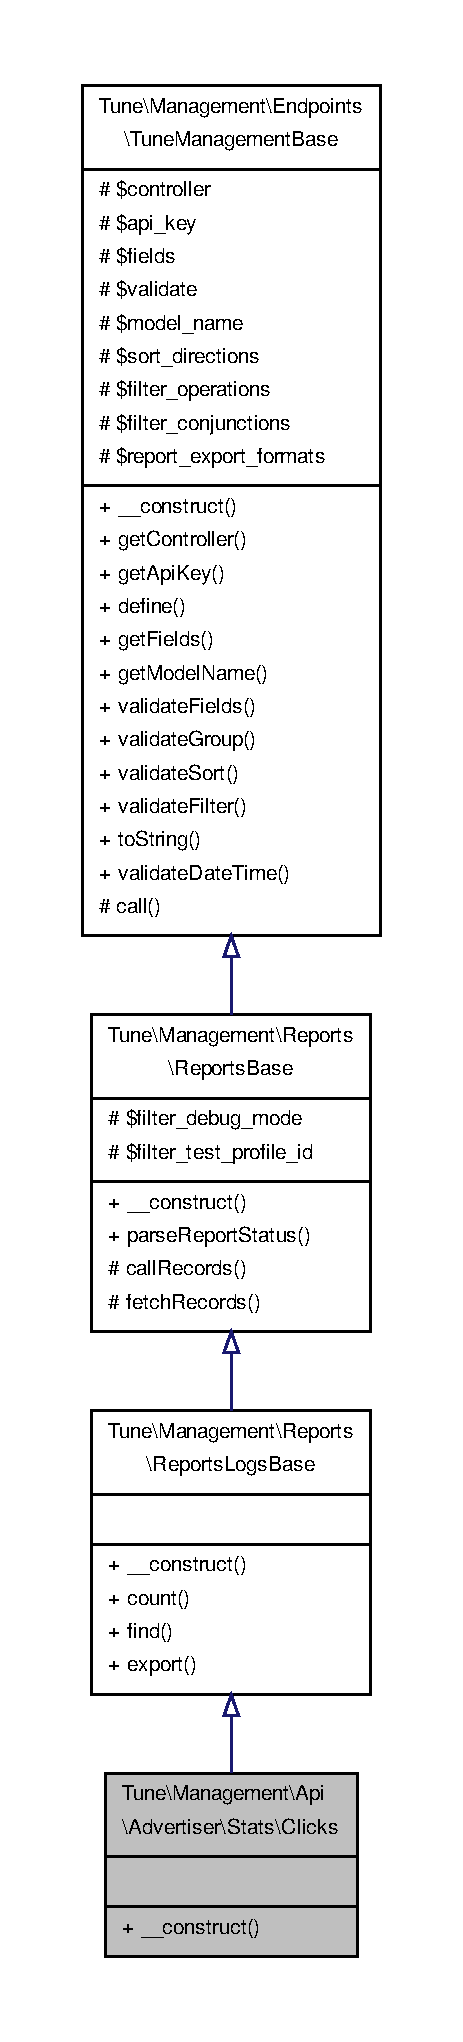
\includegraphics[height=550pt]{classTune_1_1Management_1_1Api_1_1Advertiser_1_1Stats_1_1Clicks__inherit__graph}
\end{center}
\end{figure}


Collaboration diagram for Tune\textbackslash{}Management\textbackslash{}Api\textbackslash{}Advertiser\textbackslash{}Stats\textbackslash{}Clicks\-:
\nopagebreak
\begin{figure}[H]
\begin{center}
\leavevmode
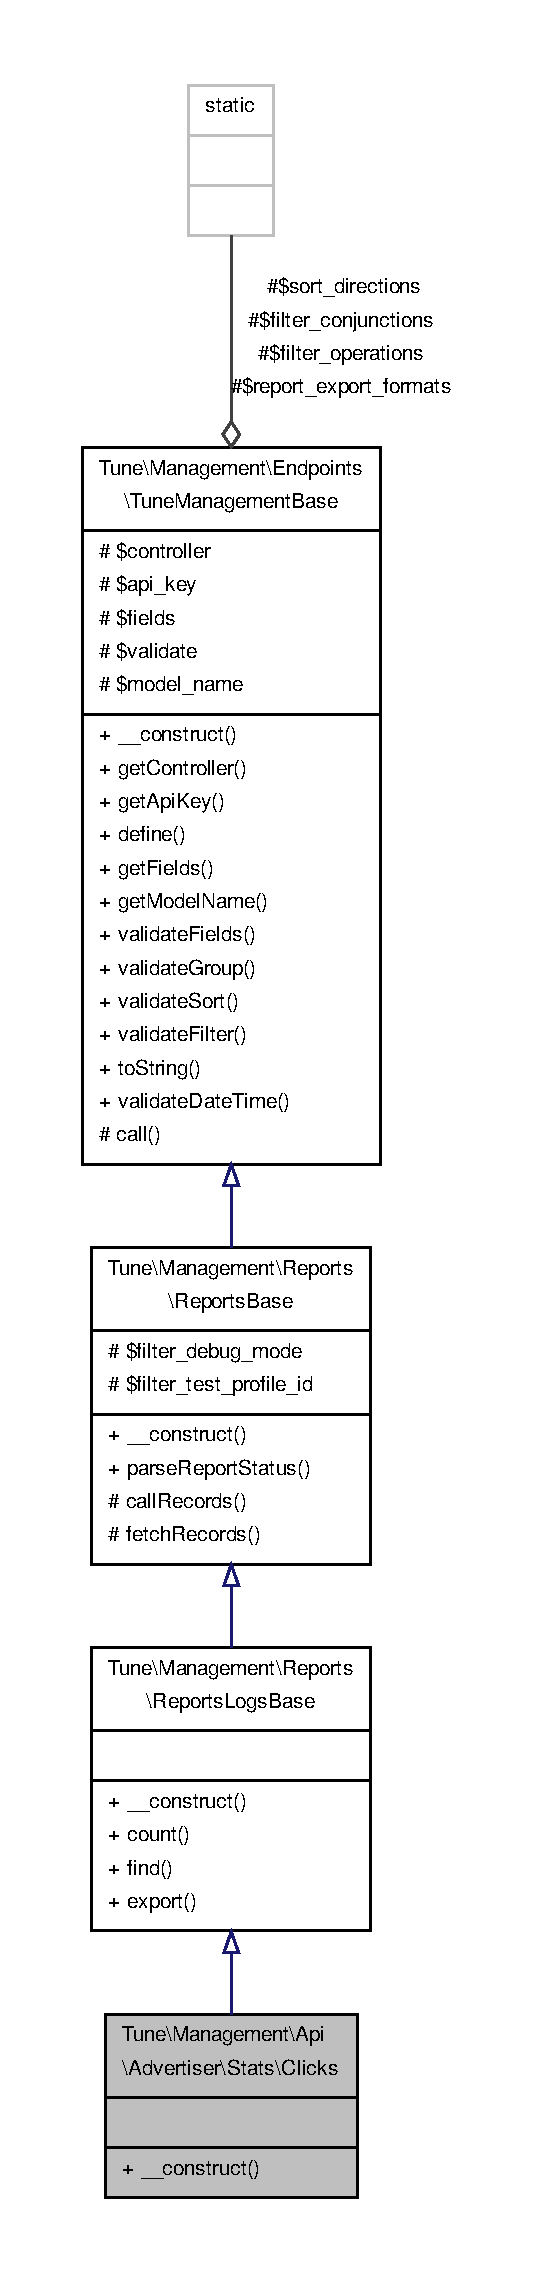
\includegraphics[height=550pt]{classTune_1_1Management_1_1Api_1_1Advertiser_1_1Stats_1_1Clicks__coll__graph}
\end{center}
\end{figure}
\subsection*{Public Member Functions}
\begin{DoxyCompactItemize}
\item 
\hyperlink{classTune_1_1Management_1_1Api_1_1Advertiser_1_1Stats_1_1Clicks_abe1281b3ed7eb41663890de320083845}{\-\_\-\-\_\-construct} (\$api\-\_\-key, \$validate=false)
\begin{DoxyCompactList}\small\item\em Constructor. \end{DoxyCompactList}\end{DoxyCompactItemize}
\subsection*{Additional Inherited Members}


\subsection{Detailed Description}
\begin{Desc}
\item[Examples\-: ]\par
\hyperlink{ExampleClicks_8php-example}{Example\-Clicks.\-php}.\end{Desc}


Definition at line 48 of file Clicks.\-php.



\subsection{Constructor \& Destructor Documentation}
\hypertarget{classTune_1_1Management_1_1Api_1_1Advertiser_1_1Stats_1_1Clicks_abe1281b3ed7eb41663890de320083845}{\index{Tune\-::\-Management\-::\-Api\-::\-Advertiser\-::\-Stats\-::\-Clicks@{Tune\-::\-Management\-::\-Api\-::\-Advertiser\-::\-Stats\-::\-Clicks}!\-\_\-\-\_\-construct@{\-\_\-\-\_\-construct}}
\index{\-\_\-\-\_\-construct@{\-\_\-\-\_\-construct}!Tune::Management::Api::Advertiser::Stats::Clicks@{Tune\-::\-Management\-::\-Api\-::\-Advertiser\-::\-Stats\-::\-Clicks}}
\subsubsection[{\-\_\-\-\_\-construct}]{\setlength{\rightskip}{0pt plus 5cm}Tune\textbackslash{}\-Management\textbackslash{}\-Api\textbackslash{}\-Advertiser\textbackslash{}\-Stats\textbackslash{}\-Clicks\-::\-\_\-\-\_\-construct (
\begin{DoxyParamCaption}
\item[{}]{\$api\-\_\-key, }
\item[{}]{\$validate = {\ttfamily false}}
\end{DoxyParamCaption}
)}}\label{classTune_1_1Management_1_1Api_1_1Advertiser_1_1Stats_1_1Clicks_abe1281b3ed7eb41663890de320083845}


Constructor. 


\begin{DoxyParams}[1]{Parameters}
string & {\em \$api\-\_\-key} & \hyperlink{namespaceTune}{Tune} Mobile\-App\-Tracking A\-P\-I Key. \\
\hline
bool & {\em \$validate} & Validate fields used by actions' parameters. \\
\hline
\end{DoxyParams}


Definition at line 56 of file Clicks.\-php.


\begin{DoxyCode}
59       \{
60         parent::\_\_construct(
61             \textcolor{stringliteral}{"advertiser/stats/clicks"},
62             \hyperlink{classTune_1_1Management_1_1Endpoints_1_1TuneManagementBase_ac53649b4bc72055e1d55e53e0b6f244e}{$api\_key},
63             \hyperlink{classTune_1_1Management_1_1Endpoints_1_1TuneManagementBase_a264eed27b0a1c963808fc7eab6da98bc}{$validate},
64             \hyperlink{classTune_1_1Management_1_1Reports_1_1ReportsBase_a6dde408a407042ce3f665e9f16f386b1}{$filter\_debug\_mode} = \textcolor{keyword}{true},
65             \hyperlink{classTune_1_1Management_1_1Reports_1_1ReportsBase_a2a621a3704fdccb98094c2f94bc6180e}{$filter\_test\_profile\_id} = \textcolor{keyword}{true}
66         );
67     \}
\end{DoxyCode}


The documentation for this class was generated from the following file\-:\begin{DoxyCompactItemize}
\item 
lib/\-Tune/\-Management/\-Api/\-Advertiser/\-Stats/\hyperlink{Clicks_8php}{Clicks.\-php}\end{DoxyCompactItemize}

\hypertarget{classTune_1_1Management_1_1Api_1_1Advertiser_1_1Stats_1_1EventItems}{\section{Tune\textbackslash{}Management\textbackslash{}Api\textbackslash{}Advertiser\textbackslash{}Stats\textbackslash{}Event\-Items Class Reference}
\label{classTune_1_1Management_1_1Api_1_1Advertiser_1_1Stats_1_1EventItems}\index{Tune\textbackslash{}\-Management\textbackslash{}\-Api\textbackslash{}\-Advertiser\textbackslash{}\-Stats\textbackslash{}\-Event\-Items@{Tune\textbackslash{}\-Management\textbackslash{}\-Api\textbackslash{}\-Advertiser\textbackslash{}\-Stats\textbackslash{}\-Event\-Items}}
}


Inheritance diagram for Tune\textbackslash{}Management\textbackslash{}Api\textbackslash{}Advertiser\textbackslash{}Stats\textbackslash{}Event\-Items\-:
\nopagebreak
\begin{figure}[H]
\begin{center}
\leavevmode
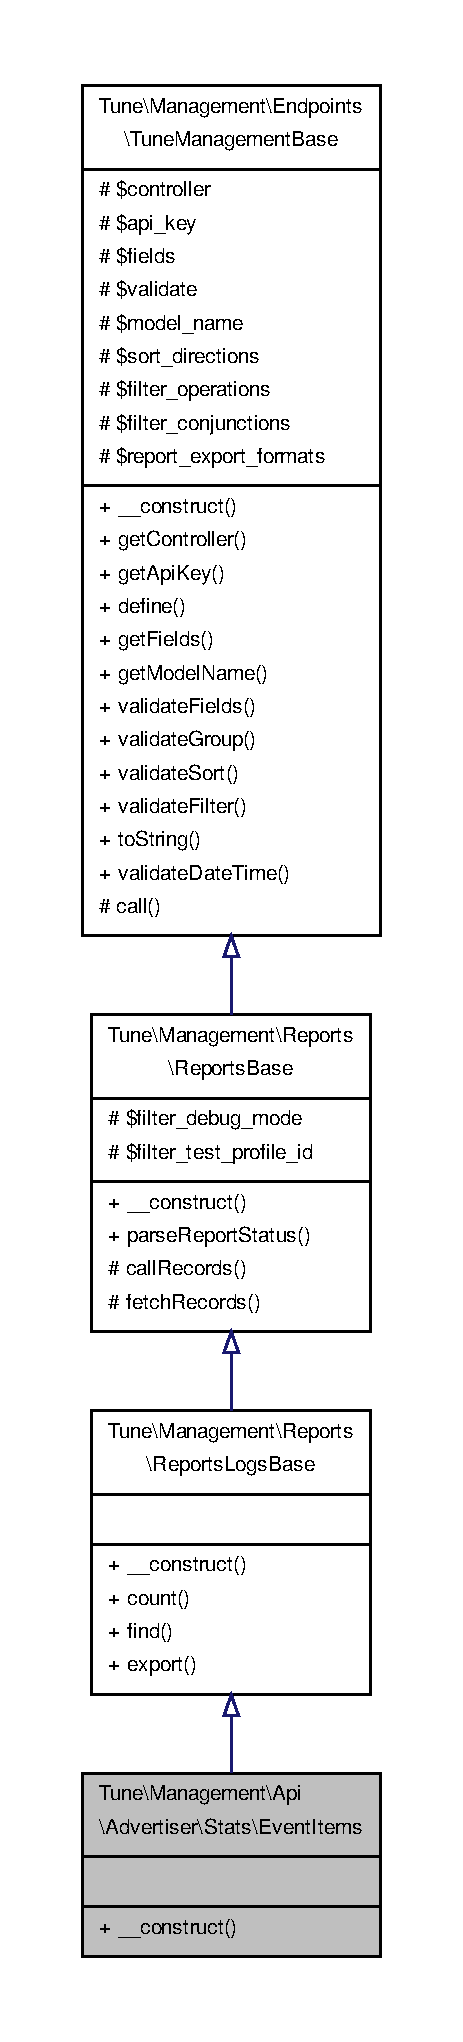
\includegraphics[height=550pt]{classTune_1_1Management_1_1Api_1_1Advertiser_1_1Stats_1_1EventItems__inherit__graph}
\end{center}
\end{figure}


Collaboration diagram for Tune\textbackslash{}Management\textbackslash{}Api\textbackslash{}Advertiser\textbackslash{}Stats\textbackslash{}Event\-Items\-:
\nopagebreak
\begin{figure}[H]
\begin{center}
\leavevmode
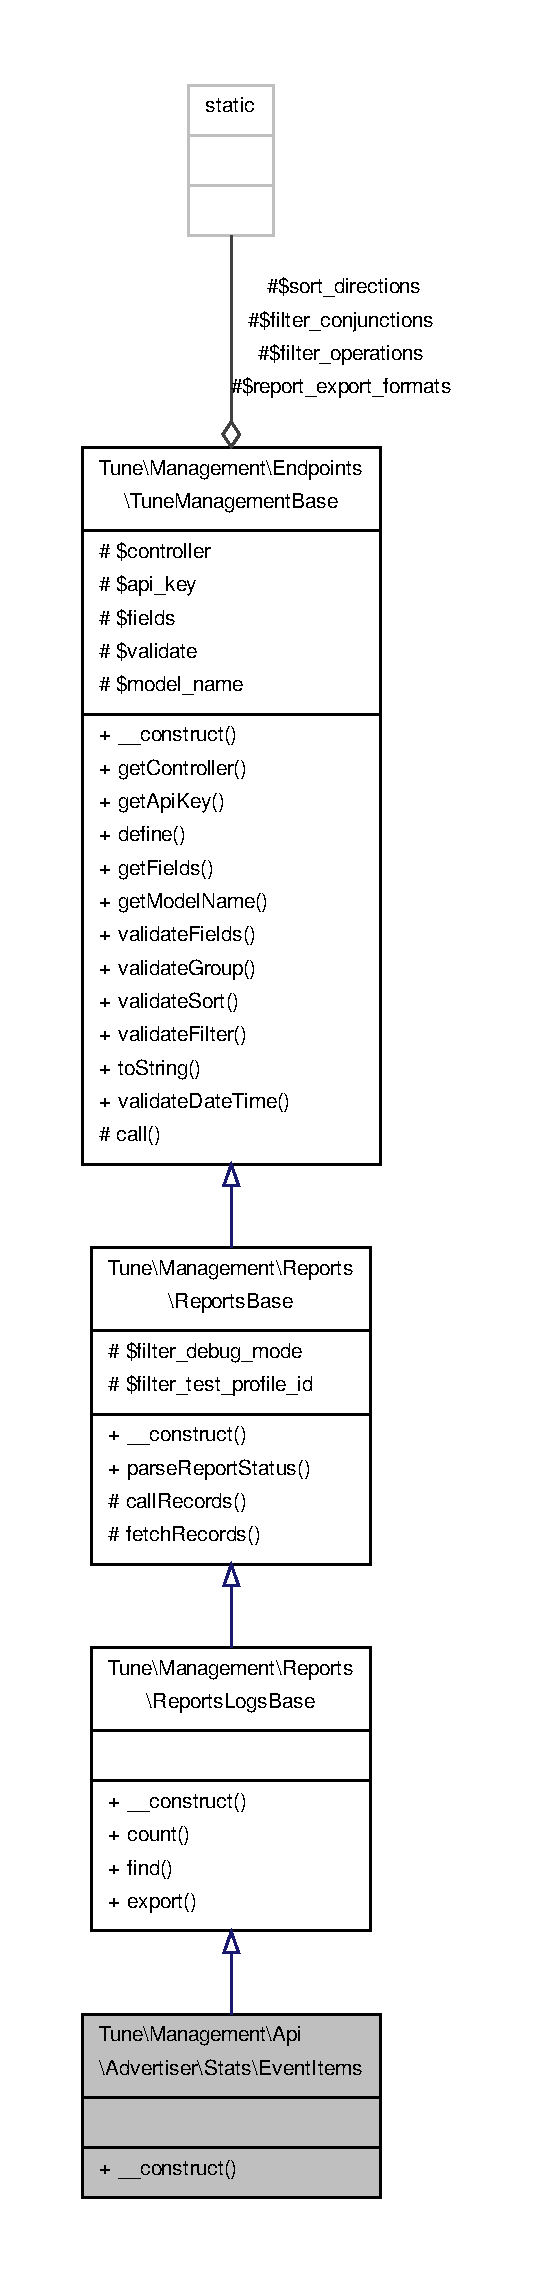
\includegraphics[height=550pt]{classTune_1_1Management_1_1Api_1_1Advertiser_1_1Stats_1_1EventItems__coll__graph}
\end{center}
\end{figure}
\subsection*{Public Member Functions}
\begin{DoxyCompactItemize}
\item 
\hyperlink{classTune_1_1Management_1_1Api_1_1Advertiser_1_1Stats_1_1EventItems_a2df85aeb94c0ab29d2b76460687b776d}{\-\_\-\-\_\-construct} (\$api\-\_\-key, \$validate=false)
\begin{DoxyCompactList}\small\item\em Constructor. \end{DoxyCompactList}\end{DoxyCompactItemize}
\subsection*{Additional Inherited Members}


\subsection{Detailed Description}
\begin{Desc}
\item[Examples\-: ]\par
\hyperlink{ExampleEventItems_8php-example}{Example\-Event\-Items.\-php}.\end{Desc}


Definition at line 49 of file Event\-Items.\-php.



\subsection{Constructor \& Destructor Documentation}
\hypertarget{classTune_1_1Management_1_1Api_1_1Advertiser_1_1Stats_1_1EventItems_a2df85aeb94c0ab29d2b76460687b776d}{\index{Tune\-::\-Management\-::\-Api\-::\-Advertiser\-::\-Stats\-::\-Event\-Items@{Tune\-::\-Management\-::\-Api\-::\-Advertiser\-::\-Stats\-::\-Event\-Items}!\-\_\-\-\_\-construct@{\-\_\-\-\_\-construct}}
\index{\-\_\-\-\_\-construct@{\-\_\-\-\_\-construct}!Tune::Management::Api::Advertiser::Stats::EventItems@{Tune\-::\-Management\-::\-Api\-::\-Advertiser\-::\-Stats\-::\-Event\-Items}}
\subsubsection[{\-\_\-\-\_\-construct}]{\setlength{\rightskip}{0pt plus 5cm}Tune\textbackslash{}\-Management\textbackslash{}\-Api\textbackslash{}\-Advertiser\textbackslash{}\-Stats\textbackslash{}\-Event\-Items\-::\-\_\-\-\_\-construct (
\begin{DoxyParamCaption}
\item[{}]{\$api\-\_\-key, }
\item[{}]{\$validate = {\ttfamily false}}
\end{DoxyParamCaption}
)}}\label{classTune_1_1Management_1_1Api_1_1Advertiser_1_1Stats_1_1EventItems_a2df85aeb94c0ab29d2b76460687b776d}


Constructor. 


\begin{DoxyParams}[1]{Parameters}
string & {\em \$api\-\_\-key} & \hyperlink{namespaceTune}{Tune} Mobile\-App\-Tracking A\-P\-I Key. \\
\hline
bool & {\em \$validate} & Validate fields used by actions' parameters. \\
\hline
\end{DoxyParams}


Definition at line 57 of file Event\-Items.\-php.


\begin{DoxyCode}
60       \{
61         parent::\_\_construct(
62             \textcolor{stringliteral}{"advertiser/stats/event/items"},
63             \hyperlink{classTune_1_1Management_1_1Endpoints_1_1TuneManagementBase_ac53649b4bc72055e1d55e53e0b6f244e}{$api\_key},
64             \hyperlink{classTune_1_1Management_1_1Reports_1_1ReportsBase_a6dde408a407042ce3f665e9f16f386b1}{$filter\_debug\_mode} = \textcolor{keyword}{false},
65             \hyperlink{classTune_1_1Management_1_1Reports_1_1ReportsBase_a2a621a3704fdccb98094c2f94bc6180e}{$filter\_test\_profile\_id} = \textcolor{keyword}{true}
66         );
67     \}
\end{DoxyCode}


The documentation for this class was generated from the following file\-:\begin{DoxyCompactItemize}
\item 
lib/\-Tune/\-Management/\-Api/\-Advertiser/\-Stats/\hyperlink{EventItems_8php}{Event\-Items.\-php}\end{DoxyCompactItemize}

\hypertarget{classTune_1_1Management_1_1Api_1_1Advertiser_1_1Stats_1_1Events}{\section{Tune\textbackslash{}Management\textbackslash{}Api\textbackslash{}Advertiser\textbackslash{}Stats\textbackslash{}Events Class Reference}
\label{classTune_1_1Management_1_1Api_1_1Advertiser_1_1Stats_1_1Events}\index{Tune\textbackslash{}\-Management\textbackslash{}\-Api\textbackslash{}\-Advertiser\textbackslash{}\-Stats\textbackslash{}\-Events@{Tune\textbackslash{}\-Management\textbackslash{}\-Api\textbackslash{}\-Advertiser\textbackslash{}\-Stats\textbackslash{}\-Events}}
}


Inheritance diagram for Tune\textbackslash{}Management\textbackslash{}Api\textbackslash{}Advertiser\textbackslash{}Stats\textbackslash{}Events\-:
\nopagebreak
\begin{figure}[H]
\begin{center}
\leavevmode
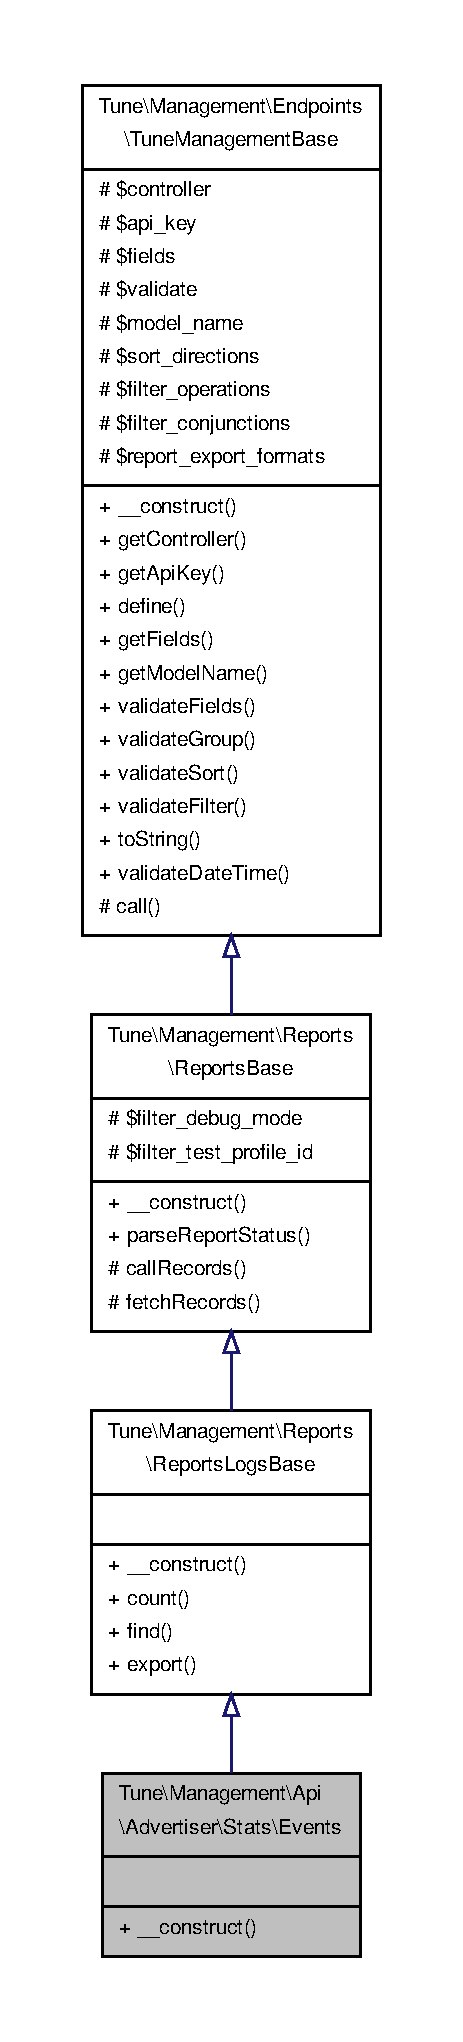
\includegraphics[height=550pt]{classTune_1_1Management_1_1Api_1_1Advertiser_1_1Stats_1_1Events__inherit__graph}
\end{center}
\end{figure}


Collaboration diagram for Tune\textbackslash{}Management\textbackslash{}Api\textbackslash{}Advertiser\textbackslash{}Stats\textbackslash{}Events\-:
\nopagebreak
\begin{figure}[H]
\begin{center}
\leavevmode
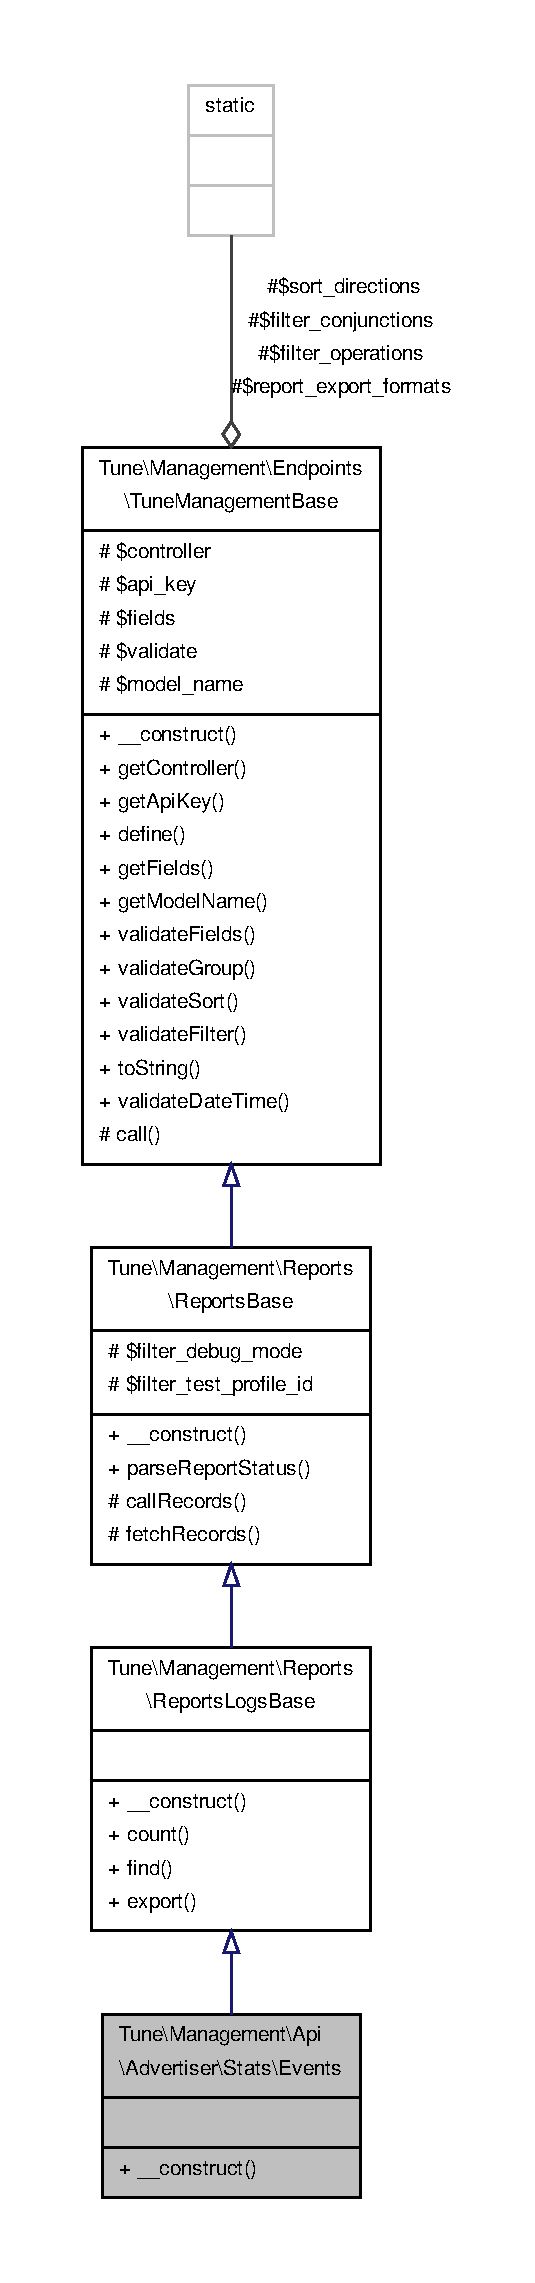
\includegraphics[height=550pt]{classTune_1_1Management_1_1Api_1_1Advertiser_1_1Stats_1_1Events__coll__graph}
\end{center}
\end{figure}
\subsection*{Public Member Functions}
\begin{DoxyCompactItemize}
\item 
\hyperlink{classTune_1_1Management_1_1Api_1_1Advertiser_1_1Stats_1_1Events_ab4c9eb1f6b98f929174ba24ef68f0829}{\-\_\-\-\_\-construct} (\$api\-\_\-key, \$validate=false)
\begin{DoxyCompactList}\small\item\em Constructor. \end{DoxyCompactList}\end{DoxyCompactItemize}
\subsection*{Additional Inherited Members}


\subsection{Detailed Description}
\begin{Desc}
\item[Examples\-: ]\par
\hyperlink{ExampleEvents_8php-example}{Example\-Events.\-php}.\end{Desc}


Definition at line 48 of file Events.\-php.



\subsection{Constructor \& Destructor Documentation}
\hypertarget{classTune_1_1Management_1_1Api_1_1Advertiser_1_1Stats_1_1Events_ab4c9eb1f6b98f929174ba24ef68f0829}{\index{Tune\-::\-Management\-::\-Api\-::\-Advertiser\-::\-Stats\-::\-Events@{Tune\-::\-Management\-::\-Api\-::\-Advertiser\-::\-Stats\-::\-Events}!\-\_\-\-\_\-construct@{\-\_\-\-\_\-construct}}
\index{\-\_\-\-\_\-construct@{\-\_\-\-\_\-construct}!Tune::Management::Api::Advertiser::Stats::Events@{Tune\-::\-Management\-::\-Api\-::\-Advertiser\-::\-Stats\-::\-Events}}
\subsubsection[{\-\_\-\-\_\-construct}]{\setlength{\rightskip}{0pt plus 5cm}Tune\textbackslash{}\-Management\textbackslash{}\-Api\textbackslash{}\-Advertiser\textbackslash{}\-Stats\textbackslash{}\-Events\-::\-\_\-\-\_\-construct (
\begin{DoxyParamCaption}
\item[{}]{\$api\-\_\-key, }
\item[{}]{\$validate = {\ttfamily false}}
\end{DoxyParamCaption}
)}}\label{classTune_1_1Management_1_1Api_1_1Advertiser_1_1Stats_1_1Events_ab4c9eb1f6b98f929174ba24ef68f0829}


Constructor. 


\begin{DoxyParams}[1]{Parameters}
string & {\em \$api\-\_\-key} & \hyperlink{namespaceTune}{Tune} Mobile\-App\-Tracking A\-P\-I Key. \\
\hline
bool & {\em \$validate} & Validate fields used by actions' parameters. \\
\hline
\end{DoxyParams}


Definition at line 56 of file Events.\-php.


\begin{DoxyCode}
59       \{
60         parent::\_\_construct(
61             \textcolor{stringliteral}{"advertiser/stats/events"},
62             \hyperlink{classTune_1_1Management_1_1Endpoints_1_1TuneManagementBase_ac53649b4bc72055e1d55e53e0b6f244e}{$api\_key},
63             \hyperlink{classTune_1_1Management_1_1Reports_1_1ReportsBase_a6dde408a407042ce3f665e9f16f386b1}{$filter\_debug\_mode} = \textcolor{keyword}{true},
64             \hyperlink{classTune_1_1Management_1_1Reports_1_1ReportsBase_a2a621a3704fdccb98094c2f94bc6180e}{$filter\_test\_profile\_id} = \textcolor{keyword}{true}
65         );
66     \}
\end{DoxyCode}


The documentation for this class was generated from the following file\-:\begin{DoxyCompactItemize}
\item 
lib/\-Tune/\-Management/\-Api/\-Advertiser/\-Stats/\hyperlink{Events_8php}{Events.\-php}\end{DoxyCompactItemize}

\hypertarget{classException}{\section{Exception Class Reference}
\label{classException}\index{Exception@{Exception}}
}


Inheritance diagram for Exception\-:
\nopagebreak
\begin{figure}[H]
\begin{center}
\leavevmode
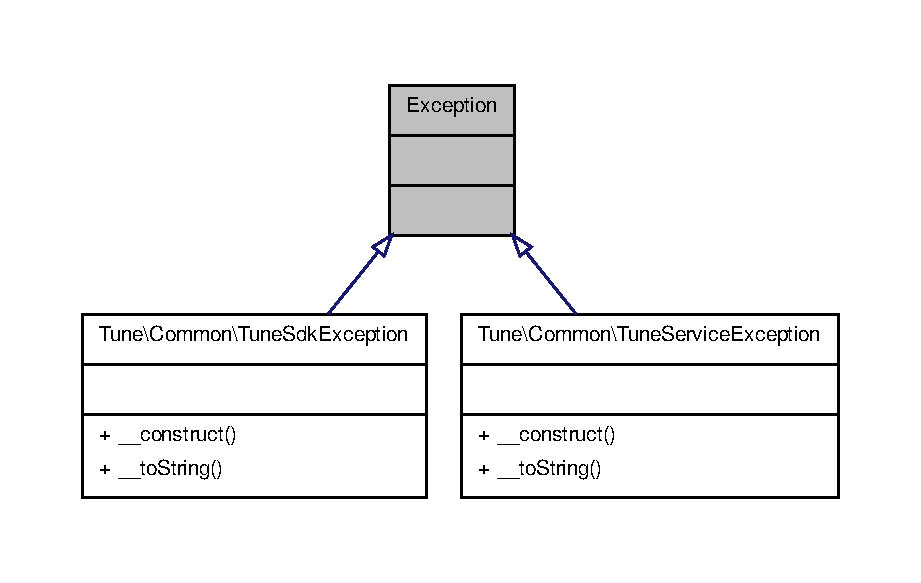
\includegraphics[width=350pt]{classException__inherit__graph}
\end{center}
\end{figure}


Collaboration diagram for Exception\-:
\nopagebreak
\begin{figure}[H]
\begin{center}
\leavevmode
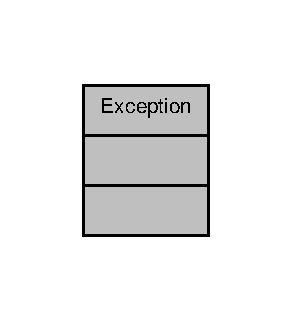
\includegraphics[width=140pt]{classException__coll__graph}
\end{center}
\end{figure}


\subsection{Detailed Description}
\begin{Desc}
\item[Examples\-: ]\par
\hyperlink{ExampleActuals_8php-example}{Example\-Actuals.\-php}, \hyperlink{ExampleClicks_8php-example}{Example\-Clicks.\-php}, \hyperlink{ExampleClient_8php-example}{Example\-Client.\-php}, \hyperlink{ExampleCohort_8php-example}{Example\-Cohort.\-php}, \hyperlink{ExampleEventItems_8php-example}{Example\-Event\-Items.\-php}, \hyperlink{ExampleEvents_8php-example}{Example\-Events.\-php}, \hyperlink{ExampleInstalls_8php-example}{Example\-Installs.\-php}, \hyperlink{ExamplePostbackUrls_8php-example}{Example\-Postback\-Urls.\-php}, \hyperlink{ExampleRetention_8php-example}{Example\-Retention.\-php}, \hyperlink{ExampleUpdates_8php-example}{Example\-Updates.\-php}, \hyperlink{ExampleUsers_8php-example}{Example\-Users.\-php}, and \hyperlink{UnittestUsers_8php-example}{Unittest\-Users.\-php}.\end{Desc}


The documentation for this class was generated from the following file\-:\begin{DoxyCompactItemize}
\item 
lib/\-Tune/\-Common/\hyperlink{TuneSdkException_8php}{Tune\-Sdk\-Exception.\-php}\end{DoxyCompactItemize}

\hypertarget{classTune_1_1Management_1_1Api_1_1Export}{\section{Tune\textbackslash{}Management\textbackslash{}Api\textbackslash{}Export Class Reference}
\label{classTune_1_1Management_1_1Api_1_1Export}\index{Tune\textbackslash{}\-Management\textbackslash{}\-Api\textbackslash{}\-Export@{Tune\textbackslash{}\-Management\textbackslash{}\-Api\textbackslash{}\-Export}}
}


Inheritance diagram for Tune\textbackslash{}Management\textbackslash{}Api\textbackslash{}Export\-:
\nopagebreak
\begin{figure}[H]
\begin{center}
\leavevmode
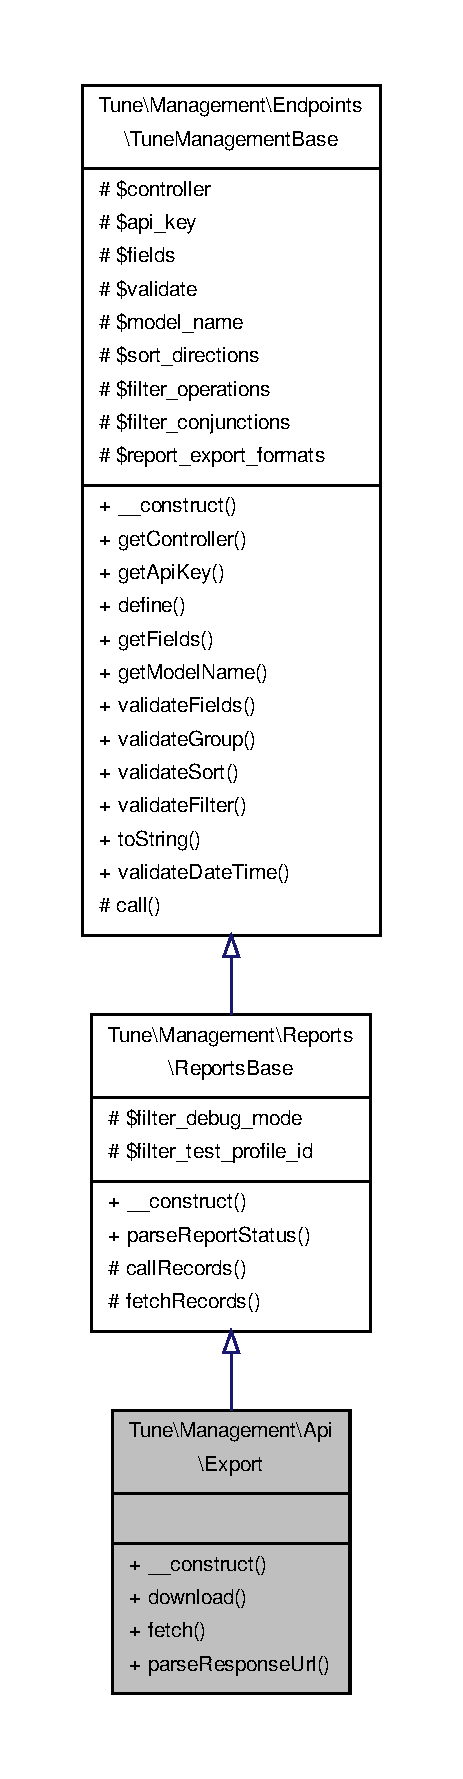
\includegraphics[height=550pt]{classTune_1_1Management_1_1Api_1_1Export__inherit__graph}
\end{center}
\end{figure}


Collaboration diagram for Tune\textbackslash{}Management\textbackslash{}Api\textbackslash{}Export\-:
\nopagebreak
\begin{figure}[H]
\begin{center}
\leavevmode
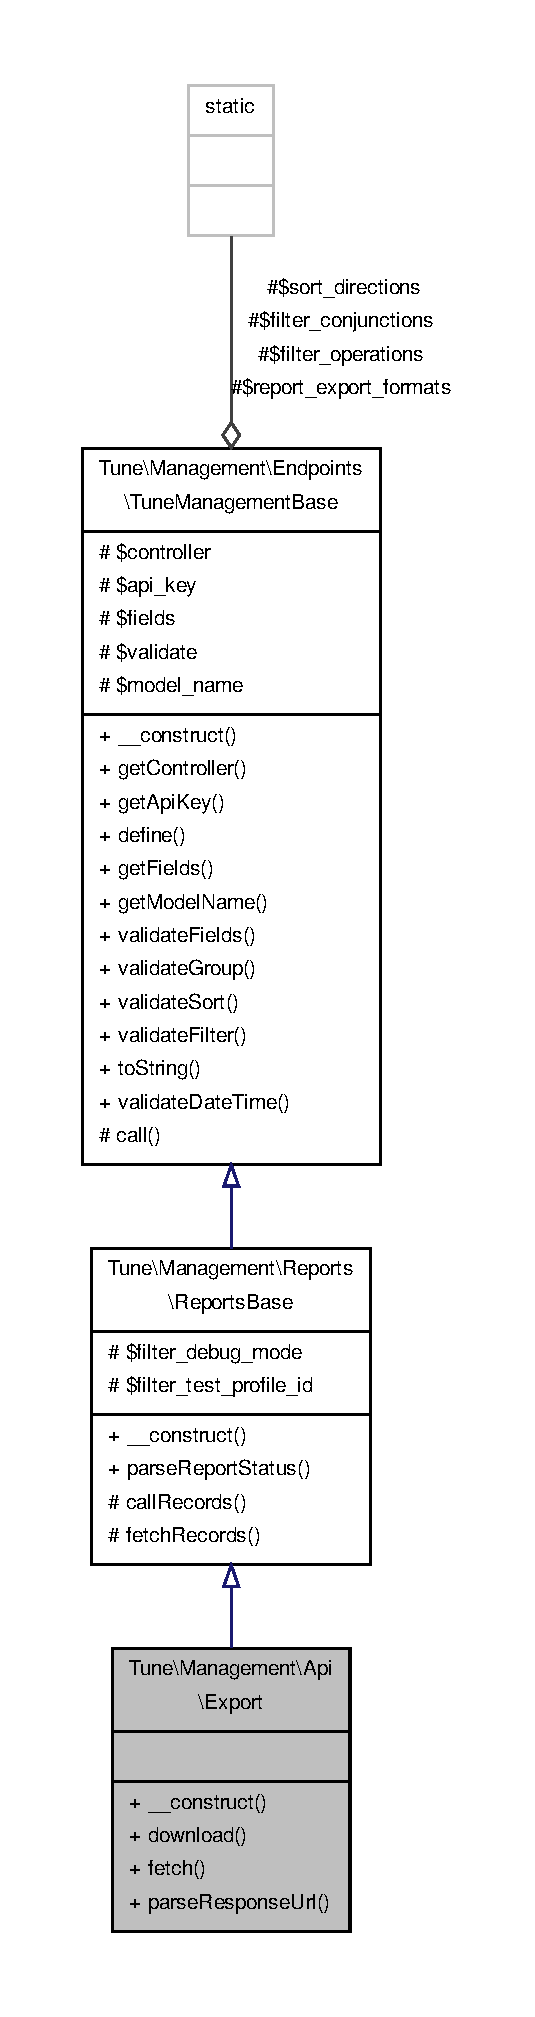
\includegraphics[height=550pt]{classTune_1_1Management_1_1Api_1_1Export__coll__graph}
\end{center}
\end{figure}
\subsection*{Public Member Functions}
\begin{DoxyCompactItemize}
\item 
\hyperlink{classTune_1_1Management_1_1Api_1_1Export_ae0da76d04bd273a61ee783f175a20b4c}{\-\_\-\-\_\-construct} (\$api\-\_\-key)
\begin{DoxyCompactList}\small\item\em Constructor. \end{DoxyCompactList}\item 
\hyperlink{classTune_1_1Management_1_1Api_1_1Export_abb9910e7ee3bdc27a6539c43df751345}{download} (\$job\-\_\-id)
\begin{DoxyCompactList}\small\item\em Action 'download' for polling export queue for status information on request report to be exported. \end{DoxyCompactList}\item 
\hyperlink{classTune_1_1Management_1_1Api_1_1Export_a74e0a671e80521e1cdc85f56c9aa7b21}{fetch} (\$job\-\_\-id, \$report\-\_\-format, \$verbose=false, \$sleep=10)
\begin{DoxyCompactList}\small\item\em Helper function for fetching report upon completion. \end{DoxyCompactList}\end{DoxyCompactItemize}
\subsection*{Static Public Member Functions}
\begin{DoxyCompactItemize}
\item 
static \hyperlink{classTune_1_1Management_1_1Api_1_1Export_a5c7222ff46e3011908de6ad5e511ce4a}{parse\-Response\-Url} (\$response)
\begin{DoxyCompactList}\small\item\em Helper function for parsing export status response to gather report url. \end{DoxyCompactList}\end{DoxyCompactItemize}
\subsection*{Additional Inherited Members}


\subsection{Detailed Description}
\begin{Desc}
\item[Examples\-: ]\par
\hyperlink{ExampleClicks_8php-example}{Example\-Clicks.\-php}, \hyperlink{ExampleEventItems_8php-example}{Example\-Event\-Items.\-php}, \hyperlink{ExampleEvents_8php-example}{Example\-Events.\-php}, \hyperlink{ExampleInstalls_8php-example}{Example\-Installs.\-php}, \hyperlink{ExamplePostbackUrls_8php-example}{Example\-Postback\-Urls.\-php}, and \hyperlink{ExampleUpdates_8php-example}{Example\-Updates.\-php}.\end{Desc}


Definition at line 51 of file Export.\-php.



\subsection{Constructor \& Destructor Documentation}
\hypertarget{classTune_1_1Management_1_1Api_1_1Export_ae0da76d04bd273a61ee783f175a20b4c}{\index{Tune\-::\-Management\-::\-Api\-::\-Export@{Tune\-::\-Management\-::\-Api\-::\-Export}!\-\_\-\-\_\-construct@{\-\_\-\-\_\-construct}}
\index{\-\_\-\-\_\-construct@{\-\_\-\-\_\-construct}!Tune::Management::Api::Export@{Tune\-::\-Management\-::\-Api\-::\-Export}}
\subsubsection[{\-\_\-\-\_\-construct}]{\setlength{\rightskip}{0pt plus 5cm}Tune\textbackslash{}\-Management\textbackslash{}\-Api\textbackslash{}\-Export\-::\-\_\-\-\_\-construct (
\begin{DoxyParamCaption}
\item[{}]{\$api\-\_\-key}
\end{DoxyParamCaption}
)}}\label{classTune_1_1Management_1_1Api_1_1Export_ae0da76d04bd273a61ee783f175a20b4c}


Constructor. 


\begin{DoxyParams}[1]{Parameters}
string & {\em \$api\-\_\-key} & Mobile\-App\-Tracking A\-P\-I Key \\
\hline
\end{DoxyParams}


Definition at line 58 of file Export.\-php.


\begin{DoxyCode}
60       \{
61         \textcolor{comment}{// api key}
62         \textcolor{keywordflow}{if} (!is\_string(\hyperlink{classTune_1_1Management_1_1Endpoints_1_1TuneManagementBase_ac53649b4bc72055e1d55e53e0b6f244e}{$api\_key}) || empty(\hyperlink{classTune_1_1Management_1_1Endpoints_1_1TuneManagementBase_ac53649b4bc72055e1d55e53e0b6f244e}{$api\_key})) \{
63             \textcolor{keywordflow}{throw} new \(\backslash\)InvalidArgumentException(\textcolor{stringliteral}{"Parameter 'api\_key' is not defined."});
64         \}
65 
66         parent::\_\_construct(
67             \hyperlink{classTune_1_1Management_1_1Endpoints_1_1TuneManagementBase_a8a73dbafcc91b04d7f1a7e2aaa9b486a}{$controller} = \textcolor{stringliteral}{"export"},
68             \hyperlink{classTune_1_1Management_1_1Endpoints_1_1TuneManagementBase_ac53649b4bc72055e1d55e53e0b6f244e}{$api\_key},
69             \hyperlink{classTune_1_1Management_1_1Reports_1_1ReportsBase_a6dde408a407042ce3f665e9f16f386b1}{$filter\_debug\_mode} = \textcolor{keyword}{false},
70             \hyperlink{classTune_1_1Management_1_1Reports_1_1ReportsBase_a2a621a3704fdccb98094c2f94bc6180e}{$filter\_test\_profile\_id} = \textcolor{keyword}{false}
71         );
72     \}
\end{DoxyCode}


\subsection{Member Function Documentation}
\hypertarget{classTune_1_1Management_1_1Api_1_1Export_abb9910e7ee3bdc27a6539c43df751345}{\index{Tune\-::\-Management\-::\-Api\-::\-Export@{Tune\-::\-Management\-::\-Api\-::\-Export}!download@{download}}
\index{download@{download}!Tune::Management::Api::Export@{Tune\-::\-Management\-::\-Api\-::\-Export}}
\subsubsection[{download}]{\setlength{\rightskip}{0pt plus 5cm}Tune\textbackslash{}\-Management\textbackslash{}\-Api\textbackslash{}\-Export\-::download (
\begin{DoxyParamCaption}
\item[{}]{\$job\-\_\-id}
\end{DoxyParamCaption}
)}}\label{classTune_1_1Management_1_1Api_1_1Export_abb9910e7ee3bdc27a6539c43df751345}


Action 'download' for polling export queue for status information on request report to be exported. 


\begin{DoxyParams}[1]{Parameters}
string & {\em \$job\-\_\-id} & Job identifier assigned for report export.\\
\hline
\end{DoxyParams}
\begin{DoxyReturn}{Returns}
object 
\end{DoxyReturn}

\begin{DoxyExceptions}{Exceptions}
{\em \textbackslash{}\-Invalid\-Argument\-Exception} & \\
\hline
\end{DoxyExceptions}


Definition at line 82 of file Export.\-php.


\begin{DoxyCode}
84       \{
85         \textcolor{keywordflow}{if} (!is\_string($job\_id) || empty($job\_id)) \{
86             \textcolor{keywordflow}{throw} new \(\backslash\)InvalidArgumentException(\textcolor{stringliteral}{"Parameter 'job\_id' is not defined."});
87         \}
88 
89         \textcolor{keywordflow}{return} parent::call(
90             $action = \textcolor{stringliteral}{"download"},
91             $query\_string\_dict = array (
92                 \textcolor{stringliteral}{'job\_id'} => $job\_id
93             )
94         );
95     \}
\end{DoxyCode}
\hypertarget{classTune_1_1Management_1_1Api_1_1Export_a74e0a671e80521e1cdc85f56c9aa7b21}{\index{Tune\-::\-Management\-::\-Api\-::\-Export@{Tune\-::\-Management\-::\-Api\-::\-Export}!fetch@{fetch}}
\index{fetch@{fetch}!Tune::Management::Api::Export@{Tune\-::\-Management\-::\-Api\-::\-Export}}
\subsubsection[{fetch}]{\setlength{\rightskip}{0pt plus 5cm}Tune\textbackslash{}\-Management\textbackslash{}\-Api\textbackslash{}\-Export\-::fetch (
\begin{DoxyParamCaption}
\item[{}]{\$job\-\_\-id, }
\item[{}]{\$report\-\_\-format, }
\item[{}]{\$verbose = {\ttfamily false}, }
\item[{}]{\$sleep = {\ttfamily 10}}
\end{DoxyParamCaption}
)}}\label{classTune_1_1Management_1_1Api_1_1Export_a74e0a671e80521e1cdc85f56c9aa7b21}


Helper function for fetching report upon completion. 

Starts worker thread for polling export queue.


\begin{DoxyParams}[1]{Parameters}
string & {\em \$job\-\_\-id} & Job identifier assigned for report export. \\
\hline
string & {\em \$report\-\_\-format} & Report export content format expectation\-: csv, json \\
\hline
bool & {\em \$verbose} & For debug purposes to monitor job export completion status. \\
\hline
int & {\em \$sleep} & Polling delay for checking job completion status.\\
\hline
\end{DoxyParams}
\begin{DoxyReturn}{Returns}
null 
\end{DoxyReturn}


Definition at line 108 of file Export.\-php.


\begin{DoxyCode}
113       \{
114         \textcolor{keywordflow}{if} (!is\_string($job\_id) || empty($job\_id)) \{
115             \textcolor{keywordflow}{throw} new \(\backslash\)InvalidArgumentException(\textcolor{stringliteral}{"Parameter 'job\_id' is not defined."});
116         \}
117 
118         \textcolor{keywordflow}{return} parent::fetchRecords(
119             $mod\_export\_class       = \_\_CLASS\_\_,
120             $mod\_export\_function    = \textcolor{stringliteral}{"download"},
121             $job\_id,
122             $report\_format,
123             $verbose,
124             $sleep
125         );
126     \}
\end{DoxyCode}
\hypertarget{classTune_1_1Management_1_1Api_1_1Export_a5c7222ff46e3011908de6ad5e511ce4a}{\index{Tune\-::\-Management\-::\-Api\-::\-Export@{Tune\-::\-Management\-::\-Api\-::\-Export}!parse\-Response\-Url@{parse\-Response\-Url}}
\index{parse\-Response\-Url@{parse\-Response\-Url}!Tune::Management::Api::Export@{Tune\-::\-Management\-::\-Api\-::\-Export}}
\subsubsection[{parse\-Response\-Url}]{\setlength{\rightskip}{0pt plus 5cm}static Tune\textbackslash{}\-Management\textbackslash{}\-Api\textbackslash{}\-Export\-::parse\-Response\-Url (
\begin{DoxyParamCaption}
\item[{}]{\$response}
\end{DoxyParamCaption}
)\hspace{0.3cm}{\ttfamily [static]}}}\label{classTune_1_1Management_1_1Api_1_1Export_a5c7222ff46e3011908de6ad5e511ce4a}


Helper function for parsing export status response to gather report url. 


\begin{DoxyParams}{Parameters}
{\em \$response} & \\
\hline
\end{DoxyParams}
\begin{DoxyReturn}{Returns}
mixed 
\end{DoxyReturn}

\begin{DoxyExceptions}{Exceptions}
{\em \textbackslash{}\-Invalid\-Argument\-Exception} & \\
\hline
{\em \textbackslash{}\-Tune\textbackslash{}\-Common\textbackslash{}\-Tune\-Service\-Exception} & \\
\hline
\end{DoxyExceptions}


Definition at line 137 of file Export.\-php.


\begin{DoxyCode}
139       \{
140         \textcolor{keywordflow}{if} (is\_null($response)) \{
141             \textcolor{keywordflow}{throw} new \(\backslash\)InvalidArgumentException(\textcolor{stringliteral}{"Parameter 'response' is not defined."});
142         \}
143         \textcolor{keywordflow}{if} (is\_null($response->getData())) \{
144             \textcolor{keywordflow}{throw} \textcolor{keyword}{new} TuneServiceException(\textcolor{stringliteral}{"Report request failed to get export data."});
145         \}
146         \textcolor{keywordflow}{if} (!array\_key\_exists(\textcolor{stringliteral}{"data"}, $response->getData())) \{
147             \textcolor{keywordflow}{throw} \textcolor{keyword}{new} TuneServiceException(\textcolor{stringliteral}{"Export response does not contain 'data'."});
148         \}
149         \textcolor{keywordflow}{if} (is\_null($response->getData()[\textcolor{stringliteral}{"data"}])) \{
150             \textcolor{keywordflow}{throw} \textcolor{keyword}{new} TuneServiceException(\textcolor{stringliteral}{"Export data response does not contain 'data'."});
151         \}
152         \textcolor{keywordflow}{if} (!array\_key\_exists(\textcolor{stringliteral}{"url"}, $response->getData()[\textcolor{stringliteral}{"data"}])) \{
153             \textcolor{keywordflow}{throw} \textcolor{keyword}{new} TuneServiceException(\textcolor{stringliteral}{"Export response 'data' does not contain 'url'."});
154         \}
155 
156         $report\_url = $response->getData()[\textcolor{stringliteral}{"data"}][\textcolor{stringliteral}{"url"}];
157 
158         \textcolor{keywordflow}{return} $report\_url;
159     \}
\end{DoxyCode}


The documentation for this class was generated from the following file\-:\begin{DoxyCompactItemize}
\item 
lib/\-Tune/\-Management/\-Api/\hyperlink{Export_8php}{Export.\-php}\end{DoxyCompactItemize}

\hypertarget{classTune_1_1Management_1_1Api_1_1Advertiser_1_1Stats_1_1Installs}{\section{Tune\textbackslash{}Management\textbackslash{}Api\textbackslash{}Advertiser\textbackslash{}Stats\textbackslash{}Installs Class Reference}
\label{classTune_1_1Management_1_1Api_1_1Advertiser_1_1Stats_1_1Installs}\index{Tune\textbackslash{}\-Management\textbackslash{}\-Api\textbackslash{}\-Advertiser\textbackslash{}\-Stats\textbackslash{}\-Installs@{Tune\textbackslash{}\-Management\textbackslash{}\-Api\textbackslash{}\-Advertiser\textbackslash{}\-Stats\textbackslash{}\-Installs}}
}


Inheritance diagram for Tune\textbackslash{}Management\textbackslash{}Api\textbackslash{}Advertiser\textbackslash{}Stats\textbackslash{}Installs\-:
\nopagebreak
\begin{figure}[H]
\begin{center}
\leavevmode
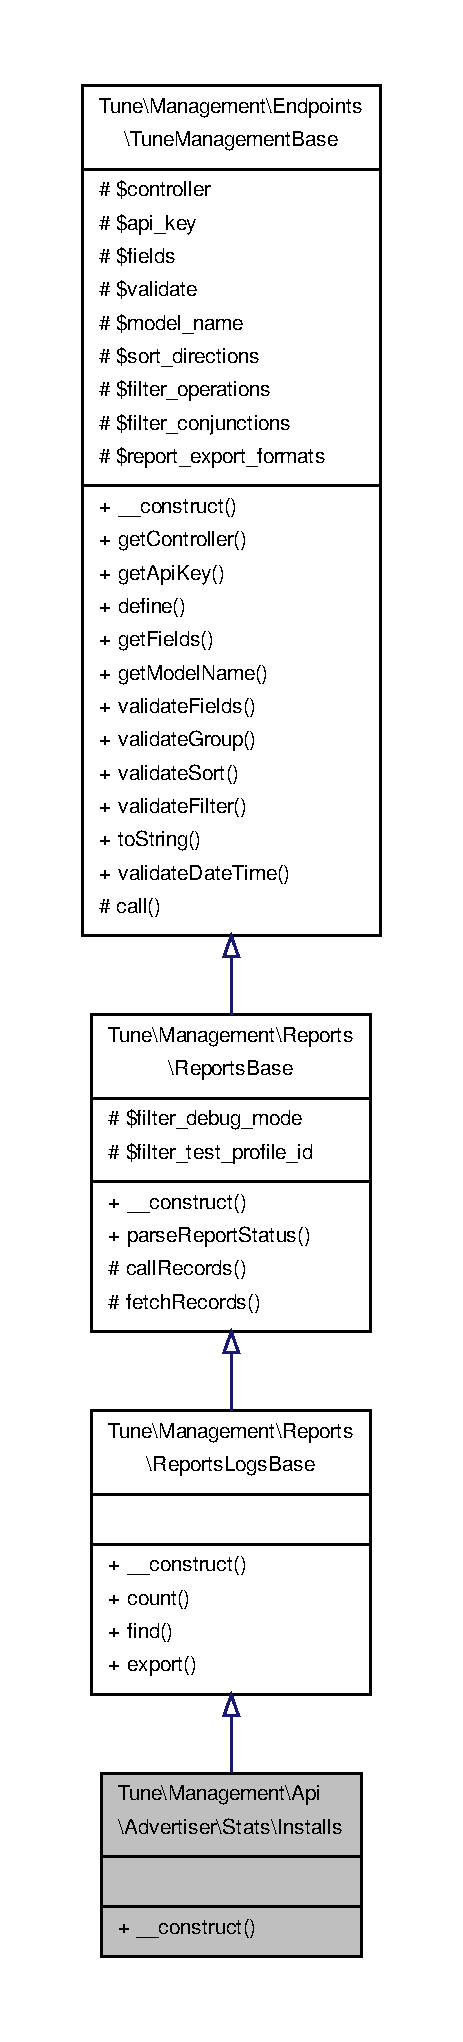
\includegraphics[height=550pt]{classTune_1_1Management_1_1Api_1_1Advertiser_1_1Stats_1_1Installs__inherit__graph}
\end{center}
\end{figure}


Collaboration diagram for Tune\textbackslash{}Management\textbackslash{}Api\textbackslash{}Advertiser\textbackslash{}Stats\textbackslash{}Installs\-:
\nopagebreak
\begin{figure}[H]
\begin{center}
\leavevmode
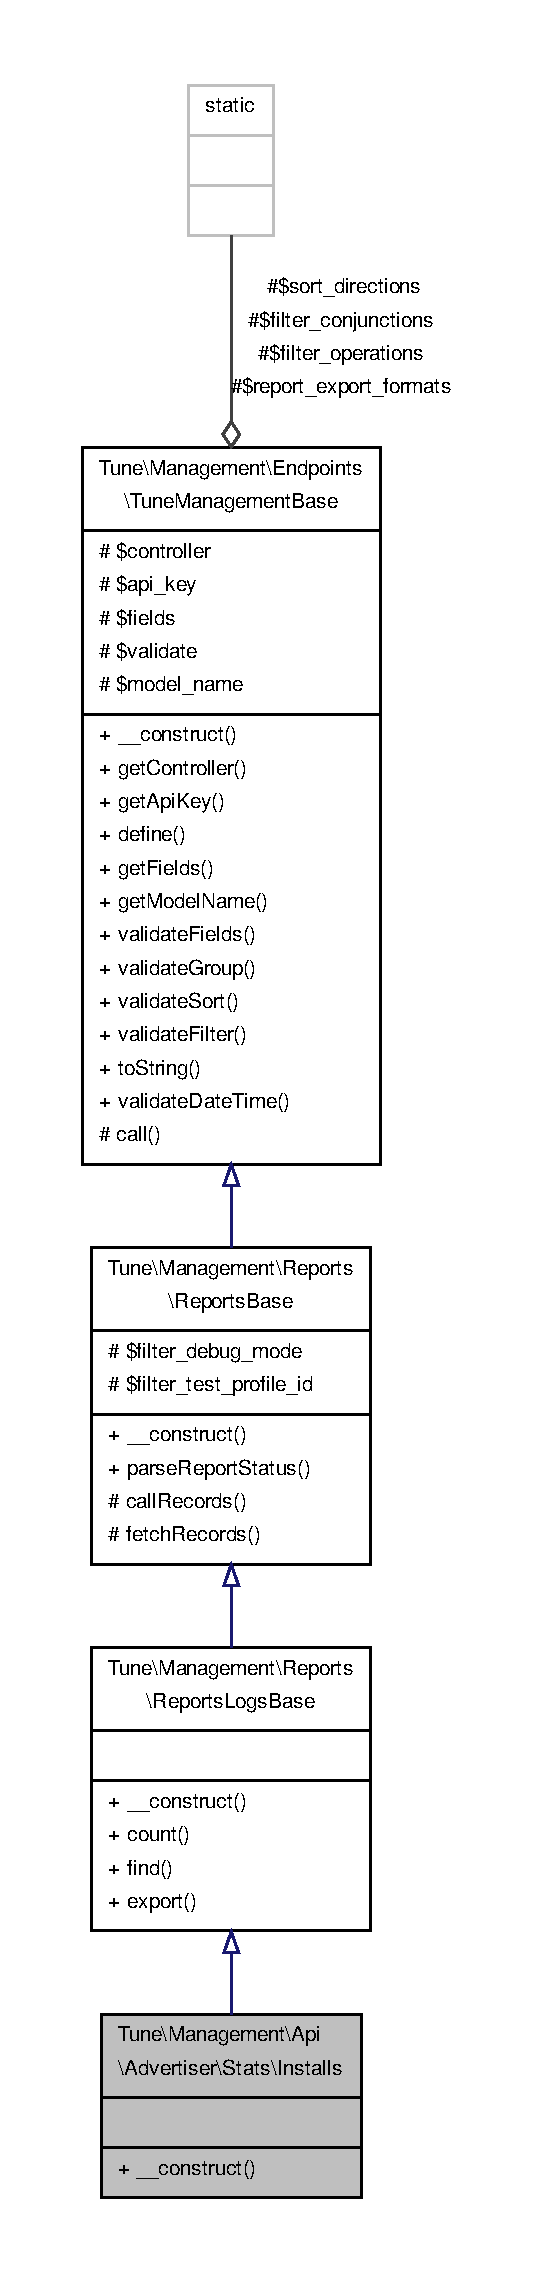
\includegraphics[height=550pt]{classTune_1_1Management_1_1Api_1_1Advertiser_1_1Stats_1_1Installs__coll__graph}
\end{center}
\end{figure}
\subsection*{Public Member Functions}
\begin{DoxyCompactItemize}
\item 
\hyperlink{classTune_1_1Management_1_1Api_1_1Advertiser_1_1Stats_1_1Installs_a45676dff8a2f948220260b7348f4d508}{\-\_\-\-\_\-construct} (\$api\-\_\-key, \$validate=false)
\begin{DoxyCompactList}\small\item\em Constructor. \end{DoxyCompactList}\end{DoxyCompactItemize}
\subsection*{Additional Inherited Members}


\subsection{Detailed Description}
\begin{Desc}
\item[Examples\-: ]\par
\hyperlink{ExampleInstalls_8php-example}{Example\-Installs.\-php}.\end{Desc}


Definition at line 48 of file Installs.\-php.



\subsection{Constructor \& Destructor Documentation}
\hypertarget{classTune_1_1Management_1_1Api_1_1Advertiser_1_1Stats_1_1Installs_a45676dff8a2f948220260b7348f4d508}{\index{Tune\-::\-Management\-::\-Api\-::\-Advertiser\-::\-Stats\-::\-Installs@{Tune\-::\-Management\-::\-Api\-::\-Advertiser\-::\-Stats\-::\-Installs}!\-\_\-\-\_\-construct@{\-\_\-\-\_\-construct}}
\index{\-\_\-\-\_\-construct@{\-\_\-\-\_\-construct}!Tune::Management::Api::Advertiser::Stats::Installs@{Tune\-::\-Management\-::\-Api\-::\-Advertiser\-::\-Stats\-::\-Installs}}
\subsubsection[{\-\_\-\-\_\-construct}]{\setlength{\rightskip}{0pt plus 5cm}Tune\textbackslash{}\-Management\textbackslash{}\-Api\textbackslash{}\-Advertiser\textbackslash{}\-Stats\textbackslash{}\-Installs\-::\-\_\-\-\_\-construct (
\begin{DoxyParamCaption}
\item[{}]{\$api\-\_\-key, }
\item[{}]{\$validate = {\ttfamily false}}
\end{DoxyParamCaption}
)}}\label{classTune_1_1Management_1_1Api_1_1Advertiser_1_1Stats_1_1Installs_a45676dff8a2f948220260b7348f4d508}


Constructor. 


\begin{DoxyParams}[1]{Parameters}
string & {\em \$api\-\_\-key} & \hyperlink{namespaceTune}{Tune} Mobile\-App\-Tracking A\-P\-I Key. \\
\hline
bool & {\em \$validate} & Validate fields used by actions' parameters. \\
\hline
\end{DoxyParams}


Definition at line 56 of file Installs.\-php.


\begin{DoxyCode}
59       \{
60         parent::\_\_construct(
61             \textcolor{stringliteral}{"advertiser/stats/installs"},
62             \hyperlink{classTune_1_1Management_1_1Endpoints_1_1TuneManagementBase_ac53649b4bc72055e1d55e53e0b6f244e}{$api\_key},
63             \hyperlink{classTune_1_1Management_1_1Reports_1_1ReportsBase_a6dde408a407042ce3f665e9f16f386b1}{$filter\_debug\_mode} = \textcolor{keyword}{true},
64             \hyperlink{classTune_1_1Management_1_1Reports_1_1ReportsBase_a2a621a3704fdccb98094c2f94bc6180e}{$filter\_test\_profile\_id} = \textcolor{keyword}{true}
65         );
66     \}
\end{DoxyCode}


The documentation for this class was generated from the following file\-:\begin{DoxyCompactItemize}
\item 
lib/\-Tune/\-Management/\-Api/\-Advertiser/\-Stats/\hyperlink{Installs_8php}{Installs.\-php}\end{DoxyCompactItemize}

\hypertarget{classTune_1_1Management_1_1Api_1_1Advertiser_1_1Stats_1_1LTV}{\section{Tune\textbackslash{}Management\textbackslash{}Api\textbackslash{}Advertiser\textbackslash{}Stats\textbackslash{}L\-T\-V Class Reference}
\label{classTune_1_1Management_1_1Api_1_1Advertiser_1_1Stats_1_1LTV}\index{Tune\textbackslash{}\-Management\textbackslash{}\-Api\textbackslash{}\-Advertiser\textbackslash{}\-Stats\textbackslash{}\-L\-T\-V@{Tune\textbackslash{}\-Management\textbackslash{}\-Api\textbackslash{}\-Advertiser\textbackslash{}\-Stats\textbackslash{}\-L\-T\-V}}
}


Inheritance diagram for Tune\textbackslash{}Management\textbackslash{}Api\textbackslash{}Advertiser\textbackslash{}Stats\textbackslash{}L\-T\-V\-:
\nopagebreak
\begin{figure}[H]
\begin{center}
\leavevmode
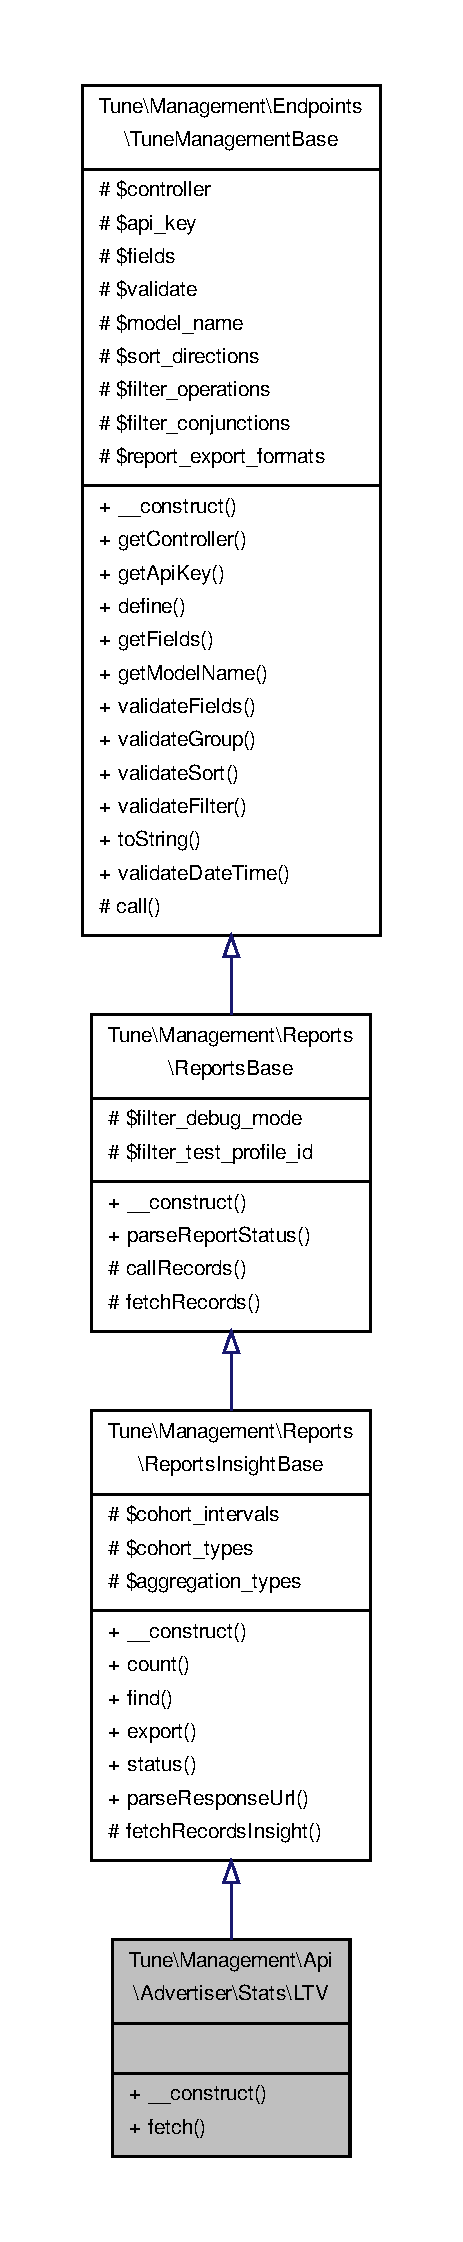
\includegraphics[height=550pt]{classTune_1_1Management_1_1Api_1_1Advertiser_1_1Stats_1_1LTV__inherit__graph}
\end{center}
\end{figure}


Collaboration diagram for Tune\textbackslash{}Management\textbackslash{}Api\textbackslash{}Advertiser\textbackslash{}Stats\textbackslash{}L\-T\-V\-:
\nopagebreak
\begin{figure}[H]
\begin{center}
\leavevmode
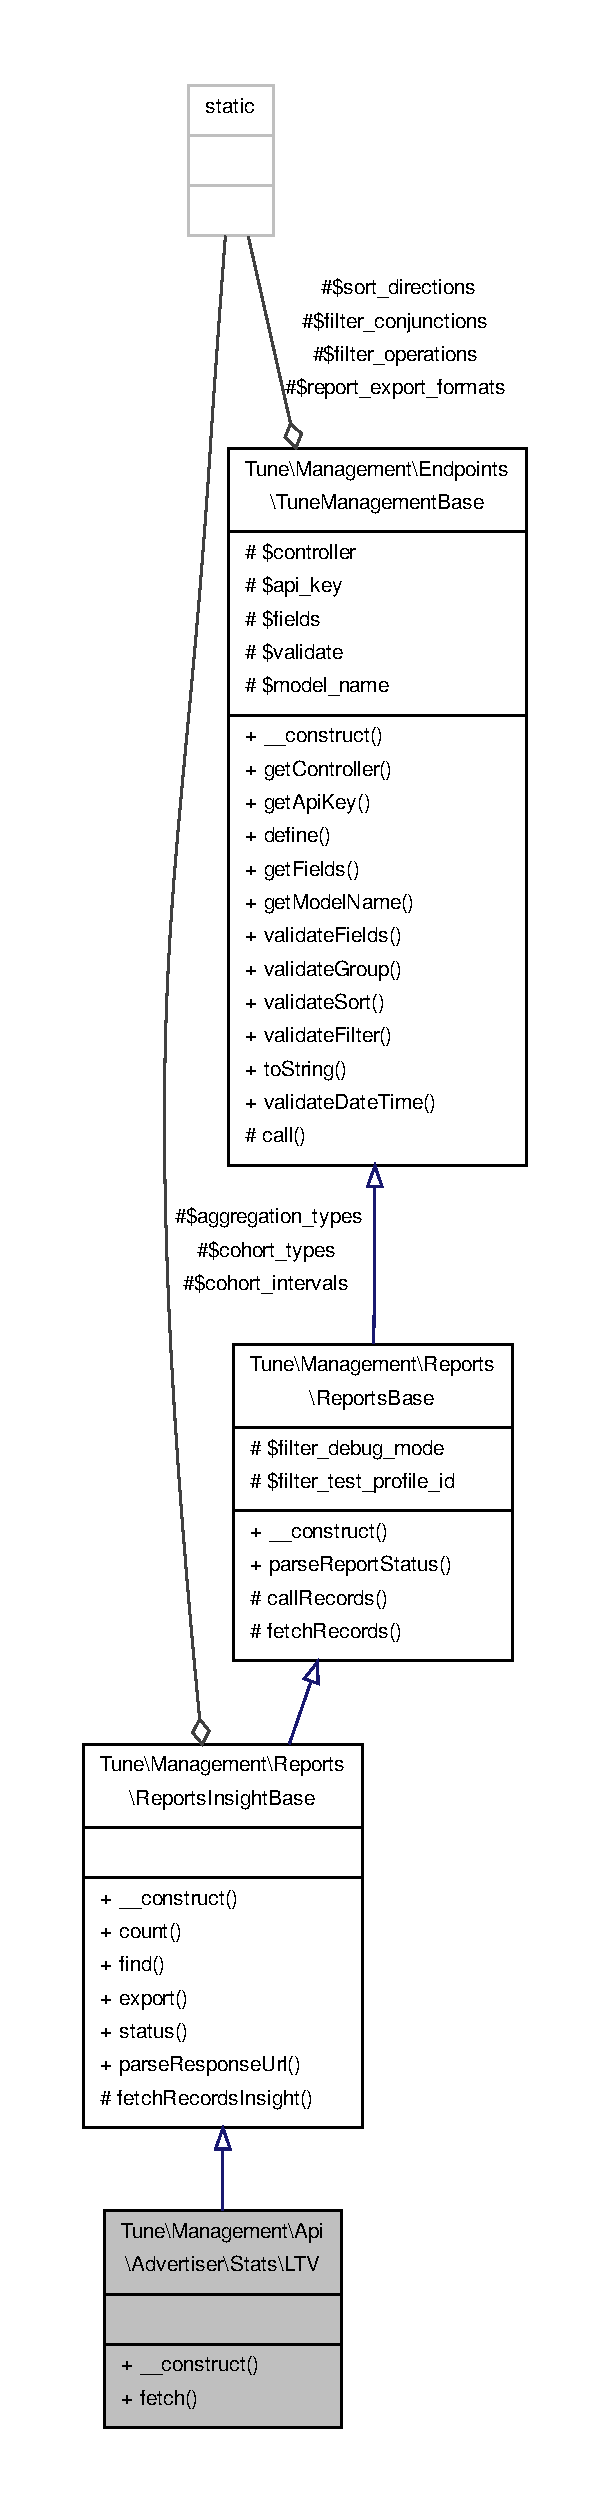
\includegraphics[height=550pt]{classTune_1_1Management_1_1Api_1_1Advertiser_1_1Stats_1_1LTV__coll__graph}
\end{center}
\end{figure}
\subsection*{Public Member Functions}
\begin{DoxyCompactItemize}
\item 
\hyperlink{classTune_1_1Management_1_1Api_1_1Advertiser_1_1Stats_1_1LTV_ac4e87ebc5c87d7a636df3103dc7fed36}{\-\_\-\-\_\-construct} (\$api\-\_\-key, \$validate=false)
\begin{DoxyCompactList}\small\item\em Constructor. \end{DoxyCompactList}\item 
\hyperlink{classTune_1_1Management_1_1Api_1_1Advertiser_1_1Stats_1_1LTV_a28cb1e1dbc9436d0a7ed319821674cea}{fetch} (\$job\-\_\-id, \$report\-\_\-format=\char`\"{}csv\char`\"{}, \$verbose=false, \$sleep=60)
\begin{DoxyCompactList}\small\item\em Helper function for fetching report document given provided job identifier. \end{DoxyCompactList}\end{DoxyCompactItemize}
\subsection*{Additional Inherited Members}


\subsection{Detailed Description}


Definition at line 48 of file L\-T\-V.\-php.



\subsection{Constructor \& Destructor Documentation}
\hypertarget{classTune_1_1Management_1_1Api_1_1Advertiser_1_1Stats_1_1LTV_ac4e87ebc5c87d7a636df3103dc7fed36}{\index{Tune\-::\-Management\-::\-Api\-::\-Advertiser\-::\-Stats\-::\-L\-T\-V@{Tune\-::\-Management\-::\-Api\-::\-Advertiser\-::\-Stats\-::\-L\-T\-V}!\-\_\-\-\_\-construct@{\-\_\-\-\_\-construct}}
\index{\-\_\-\-\_\-construct@{\-\_\-\-\_\-construct}!Tune::Management::Api::Advertiser::Stats::LTV@{Tune\-::\-Management\-::\-Api\-::\-Advertiser\-::\-Stats\-::\-L\-T\-V}}
\subsubsection[{\-\_\-\-\_\-construct}]{\setlength{\rightskip}{0pt plus 5cm}Tune\textbackslash{}\-Management\textbackslash{}\-Api\textbackslash{}\-Advertiser\textbackslash{}\-Stats\textbackslash{}\-L\-T\-V\-::\-\_\-\-\_\-construct (
\begin{DoxyParamCaption}
\item[{}]{\$api\-\_\-key, }
\item[{}]{\$validate = {\ttfamily false}}
\end{DoxyParamCaption}
)}}\label{classTune_1_1Management_1_1Api_1_1Advertiser_1_1Stats_1_1LTV_ac4e87ebc5c87d7a636df3103dc7fed36}


Constructor. 


\begin{DoxyParams}[1]{Parameters}
string & {\em \$api\-\_\-key} & \hyperlink{namespaceTune}{Tune} Mobile\-App\-Tracking A\-P\-I Key. \\
\hline
bool & {\em \$validate} & Validate fields used by actions' parameters. \\
\hline
\end{DoxyParams}


Definition at line 56 of file L\-T\-V.\-php.


\begin{DoxyCode}
59       \{
60         parent::\_\_construct(
61             \textcolor{stringliteral}{"advertiser/stats/ltv"},
62             \hyperlink{classTune_1_1Management_1_1Endpoints_1_1TuneManagementBase_ac53649b4bc72055e1d55e53e0b6f244e}{$api\_key},
63             \hyperlink{classTune_1_1Management_1_1Reports_1_1ReportsBase_a6dde408a407042ce3f665e9f16f386b1}{$filter\_debug\_mode} = \textcolor{keyword}{false},
64             \hyperlink{classTune_1_1Management_1_1Reports_1_1ReportsBase_a2a621a3704fdccb98094c2f94bc6180e}{$filter\_test\_profile\_id} = \textcolor{keyword}{true}
65         );
66     \}
\end{DoxyCode}


\subsection{Member Function Documentation}
\hypertarget{classTune_1_1Management_1_1Api_1_1Advertiser_1_1Stats_1_1LTV_a28cb1e1dbc9436d0a7ed319821674cea}{\index{Tune\-::\-Management\-::\-Api\-::\-Advertiser\-::\-Stats\-::\-L\-T\-V@{Tune\-::\-Management\-::\-Api\-::\-Advertiser\-::\-Stats\-::\-L\-T\-V}!fetch@{fetch}}
\index{fetch@{fetch}!Tune::Management::Api::Advertiser::Stats::LTV@{Tune\-::\-Management\-::\-Api\-::\-Advertiser\-::\-Stats\-::\-L\-T\-V}}
\subsubsection[{fetch}]{\setlength{\rightskip}{0pt plus 5cm}Tune\textbackslash{}\-Management\textbackslash{}\-Api\textbackslash{}\-Advertiser\textbackslash{}\-Stats\textbackslash{}\-L\-T\-V\-::fetch (
\begin{DoxyParamCaption}
\item[{}]{\$job\-\_\-id, }
\item[{}]{\$report\-\_\-format = {\ttfamily \char`\"{}csv\char`\"{}}, }
\item[{}]{\$verbose = {\ttfamily false}, }
\item[{}]{\$sleep = {\ttfamily 60}}
\end{DoxyParamCaption}
)}}\label{classTune_1_1Management_1_1Api_1_1Advertiser_1_1Stats_1_1LTV_a28cb1e1dbc9436d0a7ed319821674cea}


Helper function for fetching report document given provided job identifier. 


\begin{DoxyParams}[1]{Parameters}
string & {\em \$job\-\_\-id} & Job Identifier of report on queue. \\
\hline
string & {\em \$report\-\_\-format} & Requested document format\-: csv, json \\
\hline
bool & {\em \$verbose} & For debugging purposes only. \\
\hline
int & {\em \$sleep} & How long thread should sleep before next status request.\\
\hline
\end{DoxyParams}
\begin{DoxyReturn}{Returns}
null 
\end{DoxyReturn}


Definition at line 79 of file L\-T\-V.\-php.


\begin{DoxyCode}
84       \{
85         \textcolor{keywordflow}{return} parent::fetchRecordsInsight(
86             \_\_CLASS\_\_,
87             $job\_id,
88             $report\_format,
89             $verbose,
90             $sleep
91         );
92     \}
\end{DoxyCode}


The documentation for this class was generated from the following file\-:\begin{DoxyCompactItemize}
\item 
lib/\-Tune/\-Management/\-Api/\-Advertiser/\-Stats/\hyperlink{LTV_8php}{L\-T\-V.\-php}\end{DoxyCompactItemize}

\hypertarget{classTune_1_1Common_1_1ParenthesesParser}{\section{Tune\textbackslash{}Common\textbackslash{}Parentheses\-Parser Class Reference}
\label{classTune_1_1Common_1_1ParenthesesParser}\index{Tune\textbackslash{}\-Common\textbackslash{}\-Parentheses\-Parser@{Tune\textbackslash{}\-Common\textbackslash{}\-Parentheses\-Parser}}
}


Collaboration diagram for Tune\textbackslash{}Common\textbackslash{}Parentheses\-Parser\-:
\nopagebreak
\begin{figure}[H]
\begin{center}
\leavevmode
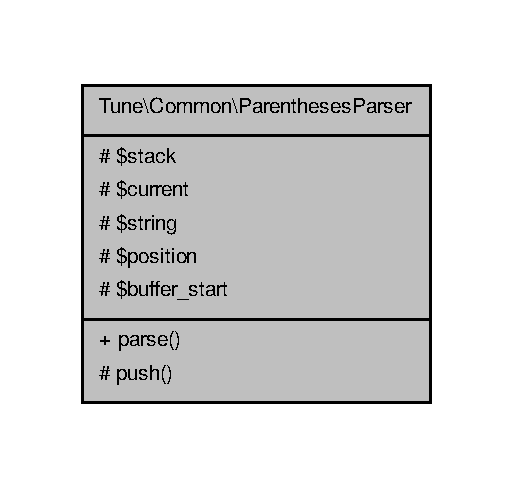
\includegraphics[width=246pt]{classTune_1_1Common_1_1ParenthesesParser__coll__graph}
\end{center}
\end{figure}
\subsection*{Public Member Functions}
\begin{DoxyCompactItemize}
\item 
\hyperlink{classTune_1_1Common_1_1ParenthesesParser_a21b2ef49db8c78bd43c7428265bb3b51}{parse} (\$string)
\begin{DoxyCompactList}\small\item\em Parse string with parentheses. \end{DoxyCompactList}\end{DoxyCompactItemize}
\subsection*{Protected Member Functions}
\begin{DoxyCompactItemize}
\item 
\hyperlink{classTune_1_1Common_1_1ParenthesesParser_a6e4681b3c7c1d5e775410706e9e08bf3}{push} ()
\begin{DoxyCompactList}\small\item\em Push parentheses element into array. \end{DoxyCompactList}\end{DoxyCompactItemize}
\subsection*{Protected Attributes}
\begin{DoxyCompactItemize}
\item 
\hyperlink{classTune_1_1Common_1_1ParenthesesParser_adcf5e7e5b906af22911f99d755e508a9}{\$stack} = null
\item 
\hyperlink{classTune_1_1Common_1_1ParenthesesParser_a1dbf6b4adbe448a5eb03ce648654138a}{\$current} = null
\item 
\hyperlink{classTune_1_1Common_1_1ParenthesesParser_ab016a5c5d09e086457c2ffebd0c0e83c}{\$string} = null
\item 
\hyperlink{classTune_1_1Common_1_1ParenthesesParser_a306af4f72762108e5a6d13357e6339d0}{\$position} = null
\item 
\hyperlink{classTune_1_1Common_1_1ParenthesesParser_a1b10c2d81217de8093d7bbff7210e9a2}{\$buffer\-\_\-start} = null
\end{DoxyCompactItemize}


\subsection{Detailed Description}


Definition at line 45 of file Parentheses\-Parser.\-php.



\subsection{Member Function Documentation}
\hypertarget{classTune_1_1Common_1_1ParenthesesParser_a21b2ef49db8c78bd43c7428265bb3b51}{\index{Tune\-::\-Common\-::\-Parentheses\-Parser@{Tune\-::\-Common\-::\-Parentheses\-Parser}!parse@{parse}}
\index{parse@{parse}!Tune::Common::ParenthesesParser@{Tune\-::\-Common\-::\-Parentheses\-Parser}}
\subsubsection[{parse}]{\setlength{\rightskip}{0pt plus 5cm}Tune\textbackslash{}\-Common\textbackslash{}\-Parentheses\-Parser\-::parse (
\begin{DoxyParamCaption}
\item[{}]{\$string}
\end{DoxyParamCaption}
)}}\label{classTune_1_1Common_1_1ParenthesesParser_a21b2ef49db8c78bd43c7428265bb3b51}


Parse string with parentheses. 


\begin{DoxyParams}{Parameters}
{\em \$string} & \\
\hline
\end{DoxyParams}
\begin{DoxyReturn}{Returns}
array 
\end{DoxyReturn}


Definition at line 65 of file Parentheses\-Parser.\-php.


\begin{DoxyCode}
66     \{
67         \textcolor{keywordflow}{if} (!\hyperlink{classTune_1_1Common_1_1ParenthesesParser_ab016a5c5d09e086457c2ffebd0c0e83c}{$string}) \{
68             \textcolor{comment}{// no string, no data}
69             \textcolor{keywordflow}{return} array();
70         \}
71 
72         \textcolor{keywordflow}{if} (\hyperlink{classTune_1_1Common_1_1ParenthesesParser_ab016a5c5d09e086457c2ffebd0c0e83c}{$string}[0] == \textcolor{charliteral}{'('}) \{
73             \textcolor{comment}{// killer outer parentheses, as they're unnecessary}
74             \hyperlink{classTune_1_1Common_1_1ParenthesesParser_ab016a5c5d09e086457c2ffebd0c0e83c}{$string} = substr(\hyperlink{classTune_1_1Common_1_1ParenthesesParser_ab016a5c5d09e086457c2ffebd0c0e83c}{$string}, 1, -1);
75         \}
76 
77         $this->current = array();
78         $this->stack = array();
79 
80         $this->\textcolor{keywordtype}{string} = \hyperlink{classTune_1_1Common_1_1ParenthesesParser_ab016a5c5d09e086457c2ffebd0c0e83c}{$string};
81         $this->length = strlen($this->\textcolor{keywordtype}{string});
82         \textcolor{comment}{// look at each character}
83         \textcolor{keywordflow}{for} ($this->position=0; $this->position < $this->length; $this->position++) \{
84             \textcolor{keywordflow}{switch} ($this->\textcolor{keywordtype}{string}[$this->position]) \{
85                 \textcolor{keywordflow}{case} \textcolor{charliteral}{'('}:
86                     $this->\hyperlink{classTune_1_1Common_1_1ParenthesesParser_a6e4681b3c7c1d5e775410706e9e08bf3}{push}();
87                     \textcolor{comment}{// push current scope to the stack an begin a new scope}
88                     array\_push($this->stack, $this->current);
89                     $this->current = array();
90                     \textcolor{keywordflow}{break};
91                 \textcolor{keywordflow}{case} \textcolor{charliteral}{')'}:
92                     $this->\hyperlink{classTune_1_1Common_1_1ParenthesesParser_a6e4681b3c7c1d5e775410706e9e08bf3}{push}();
93                     \textcolor{comment}{// save current scope}
94                     $t = \hyperlink{classTune_1_1Common_1_1ParenthesesParser_a1dbf6b4adbe448a5eb03ce648654138a}{$this->current};
95                     \textcolor{comment}{// get the last scope from stack}
96                     $this->current = array\_pop($this->stack);
97                     \textcolor{comment}{// add just saved scope to current scope}
98                     $this->current[] = $t;
99                     \textcolor{keywordflow}{break};
100                 \textcolor{comment}{/*}
101 \textcolor{comment}{                 case ' ':}
102 \textcolor{comment}{                     // make each word its own token}
103 \textcolor{comment}{                     $this->push();}
104 \textcolor{comment}{                     break;}
105 \textcolor{comment}{                 */}
106                 \textcolor{keywordflow}{default}:
107                     \textcolor{comment}{// remember the offset to do a string capture later}
108                     \textcolor{comment}{// could've also done $buffer .= $string[$position]}
109                     \textcolor{comment}{// but that would just be wasting resources…}
110                     \textcolor{keywordflow}{if} ($this->buffer\_start === null) \{
111                         $this->buffer\_start = \hyperlink{classTune_1_1Common_1_1ParenthesesParser_a306af4f72762108e5a6d13357e6339d0}{$this->position};
112                     \}
113             \}
114         \}
115 
116         \textcolor{keywordflow}{return} \hyperlink{classTune_1_1Common_1_1ParenthesesParser_a1dbf6b4adbe448a5eb03ce648654138a}{$this->current};
117     \}
\end{DoxyCode}


Here is the call graph for this function\-:
\nopagebreak
\begin{figure}[H]
\begin{center}
\leavevmode
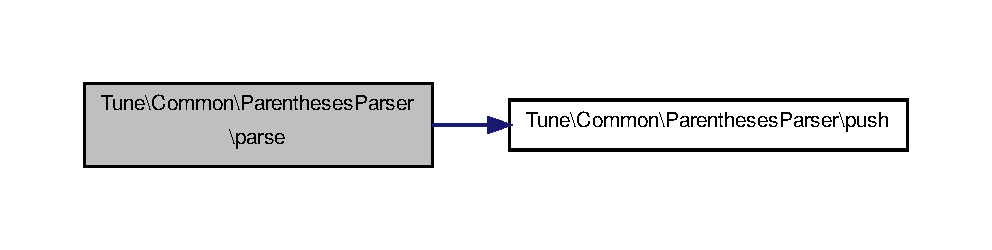
\includegraphics[width=350pt]{classTune_1_1Common_1_1ParenthesesParser_a21b2ef49db8c78bd43c7428265bb3b51_cgraph}
\end{center}
\end{figure}


\hypertarget{classTune_1_1Common_1_1ParenthesesParser_a6e4681b3c7c1d5e775410706e9e08bf3}{\index{Tune\-::\-Common\-::\-Parentheses\-Parser@{Tune\-::\-Common\-::\-Parentheses\-Parser}!push@{push}}
\index{push@{push}!Tune::Common::ParenthesesParser@{Tune\-::\-Common\-::\-Parentheses\-Parser}}
\subsubsection[{push}]{\setlength{\rightskip}{0pt plus 5cm}Tune\textbackslash{}\-Common\textbackslash{}\-Parentheses\-Parser\-::push (
\begin{DoxyParamCaption}
{}
\end{DoxyParamCaption}
)\hspace{0.3cm}{\ttfamily [protected]}}}\label{classTune_1_1Common_1_1ParenthesesParser_a6e4681b3c7c1d5e775410706e9e08bf3}


Push parentheses element into array. 



Definition at line 122 of file Parentheses\-Parser.\-php.


\begin{DoxyCode}
123     \{
124         \textcolor{keywordflow}{if} ($this->buffer\_start !== null) \{
125             \textcolor{comment}{// extract string from buffer start to current position}
126             $buffer = substr($this->\textcolor{keywordtype}{string}, $this->buffer\_start, $this->position - $this->buffer\_start);
127             \textcolor{comment}{// clean buffer}
128             $this->buffer\_start = null;
129             \textcolor{comment}{// throw token into current scope}
130             $this->current[] = $buffer;
131         \}
132     \}
\end{DoxyCode}


Here is the caller graph for this function\-:
\nopagebreak
\begin{figure}[H]
\begin{center}
\leavevmode
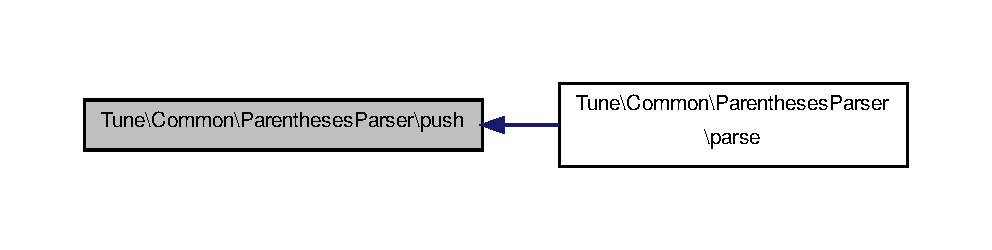
\includegraphics[width=350pt]{classTune_1_1Common_1_1ParenthesesParser_a6e4681b3c7c1d5e775410706e9e08bf3_icgraph}
\end{center}
\end{figure}




\subsection{Field Documentation}
\hypertarget{classTune_1_1Common_1_1ParenthesesParser_a1b10c2d81217de8093d7bbff7210e9a2}{\index{Tune\-::\-Common\-::\-Parentheses\-Parser@{Tune\-::\-Common\-::\-Parentheses\-Parser}!\$buffer\-\_\-start@{\$buffer\-\_\-start}}
\index{\$buffer\-\_\-start@{\$buffer\-\_\-start}!Tune::Common::ParenthesesParser@{Tune\-::\-Common\-::\-Parentheses\-Parser}}
\subsubsection[{\$buffer\-\_\-start}]{\setlength{\rightskip}{0pt plus 5cm}Tune\textbackslash{}\-Common\textbackslash{}\-Parentheses\-Parser\-::\$buffer\-\_\-start = null\hspace{0.3cm}{\ttfamily [protected]}}}\label{classTune_1_1Common_1_1ParenthesesParser_a1b10c2d81217de8093d7bbff7210e9a2}


Definition at line 57 of file Parentheses\-Parser.\-php.

\hypertarget{classTune_1_1Common_1_1ParenthesesParser_a1dbf6b4adbe448a5eb03ce648654138a}{\index{Tune\-::\-Common\-::\-Parentheses\-Parser@{Tune\-::\-Common\-::\-Parentheses\-Parser}!\$current@{\$current}}
\index{\$current@{\$current}!Tune::Common::ParenthesesParser@{Tune\-::\-Common\-::\-Parentheses\-Parser}}
\subsubsection[{\$current}]{\setlength{\rightskip}{0pt plus 5cm}Tune\textbackslash{}\-Common\textbackslash{}\-Parentheses\-Parser\-::\$current = null\hspace{0.3cm}{\ttfamily [protected]}}}\label{classTune_1_1Common_1_1ParenthesesParser_a1dbf6b4adbe448a5eb03ce648654138a}


Definition at line 50 of file Parentheses\-Parser.\-php.

\hypertarget{classTune_1_1Common_1_1ParenthesesParser_a306af4f72762108e5a6d13357e6339d0}{\index{Tune\-::\-Common\-::\-Parentheses\-Parser@{Tune\-::\-Common\-::\-Parentheses\-Parser}!\$position@{\$position}}
\index{\$position@{\$position}!Tune::Common::ParenthesesParser@{Tune\-::\-Common\-::\-Parentheses\-Parser}}
\subsubsection[{\$position}]{\setlength{\rightskip}{0pt plus 5cm}Tune\textbackslash{}\-Common\textbackslash{}\-Parentheses\-Parser\-::\$position = null\hspace{0.3cm}{\ttfamily [protected]}}}\label{classTune_1_1Common_1_1ParenthesesParser_a306af4f72762108e5a6d13357e6339d0}


Definition at line 55 of file Parentheses\-Parser.\-php.

\hypertarget{classTune_1_1Common_1_1ParenthesesParser_adcf5e7e5b906af22911f99d755e508a9}{\index{Tune\-::\-Common\-::\-Parentheses\-Parser@{Tune\-::\-Common\-::\-Parentheses\-Parser}!\$stack@{\$stack}}
\index{\$stack@{\$stack}!Tune::Common::ParenthesesParser@{Tune\-::\-Common\-::\-Parentheses\-Parser}}
\subsubsection[{\$stack}]{\setlength{\rightskip}{0pt plus 5cm}Tune\textbackslash{}\-Common\textbackslash{}\-Parentheses\-Parser\-::\$stack = null\hspace{0.3cm}{\ttfamily [protected]}}}\label{classTune_1_1Common_1_1ParenthesesParser_adcf5e7e5b906af22911f99d755e508a9}


Definition at line 48 of file Parentheses\-Parser.\-php.

\hypertarget{classTune_1_1Common_1_1ParenthesesParser_ab016a5c5d09e086457c2ffebd0c0e83c}{\index{Tune\-::\-Common\-::\-Parentheses\-Parser@{Tune\-::\-Common\-::\-Parentheses\-Parser}!\$string@{\$string}}
\index{\$string@{\$string}!Tune::Common::ParenthesesParser@{Tune\-::\-Common\-::\-Parentheses\-Parser}}
\subsubsection[{\$string}]{\setlength{\rightskip}{0pt plus 5cm}Tune\textbackslash{}\-Common\textbackslash{}\-Parentheses\-Parser\-::\$string = null\hspace{0.3cm}{\ttfamily [protected]}}}\label{classTune_1_1Common_1_1ParenthesesParser_ab016a5c5d09e086457c2ffebd0c0e83c}


Definition at line 53 of file Parentheses\-Parser.\-php.



The documentation for this class was generated from the following file\-:\begin{DoxyCompactItemize}
\item 
lib/\-Tune/\-Common/\hyperlink{ParenthesesParser_8php}{Parentheses\-Parser.\-php}\end{DoxyCompactItemize}

\hypertarget{classTune_1_1Management_1_1Api_1_1Advertiser_1_1Stats_1_1Postbacks}{\section{Tune\textbackslash{}Management\textbackslash{}Api\textbackslash{}Advertiser\textbackslash{}Stats\textbackslash{}Postbacks Class Reference}
\label{classTune_1_1Management_1_1Api_1_1Advertiser_1_1Stats_1_1Postbacks}\index{Tune\textbackslash{}\-Management\textbackslash{}\-Api\textbackslash{}\-Advertiser\textbackslash{}\-Stats\textbackslash{}\-Postbacks@{Tune\textbackslash{}\-Management\textbackslash{}\-Api\textbackslash{}\-Advertiser\textbackslash{}\-Stats\textbackslash{}\-Postbacks}}
}


Inheritance diagram for Tune\textbackslash{}Management\textbackslash{}Api\textbackslash{}Advertiser\textbackslash{}Stats\textbackslash{}Postbacks\-:
\nopagebreak
\begin{figure}[H]
\begin{center}
\leavevmode
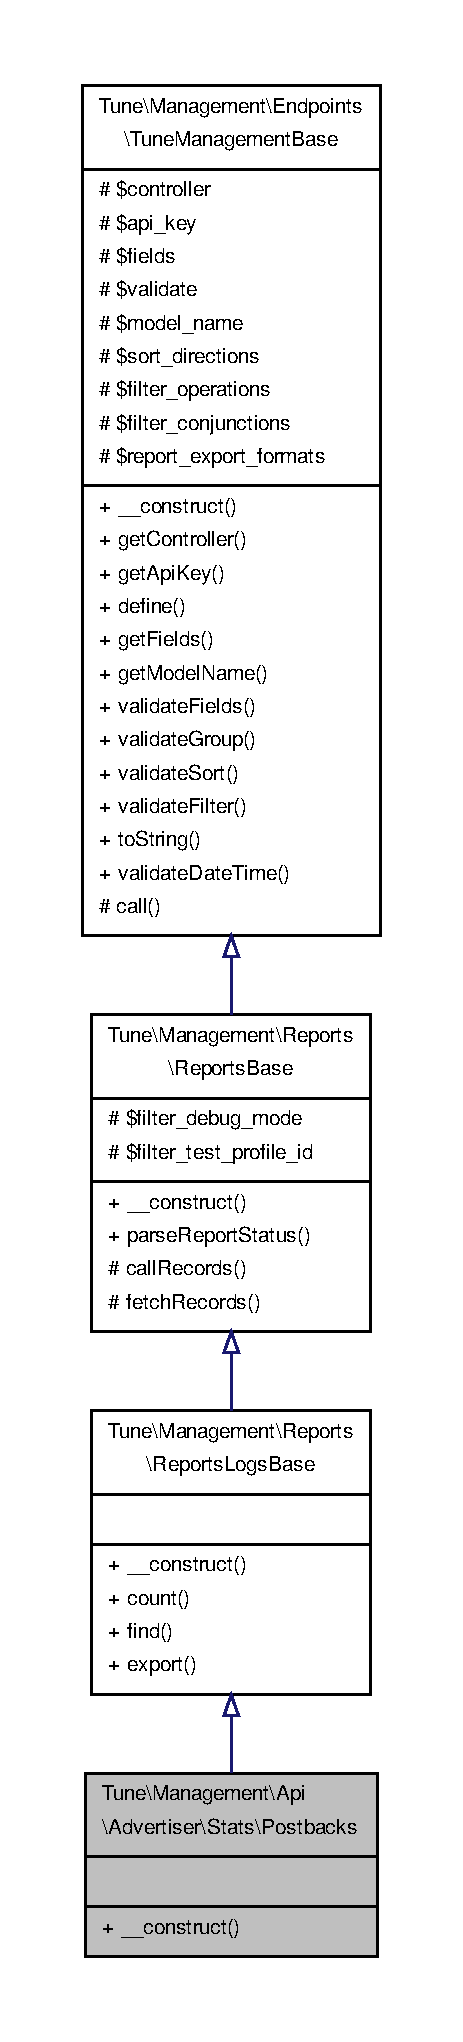
\includegraphics[height=550pt]{classTune_1_1Management_1_1Api_1_1Advertiser_1_1Stats_1_1Postbacks__inherit__graph}
\end{center}
\end{figure}


Collaboration diagram for Tune\textbackslash{}Management\textbackslash{}Api\textbackslash{}Advertiser\textbackslash{}Stats\textbackslash{}Postbacks\-:
\nopagebreak
\begin{figure}[H]
\begin{center}
\leavevmode
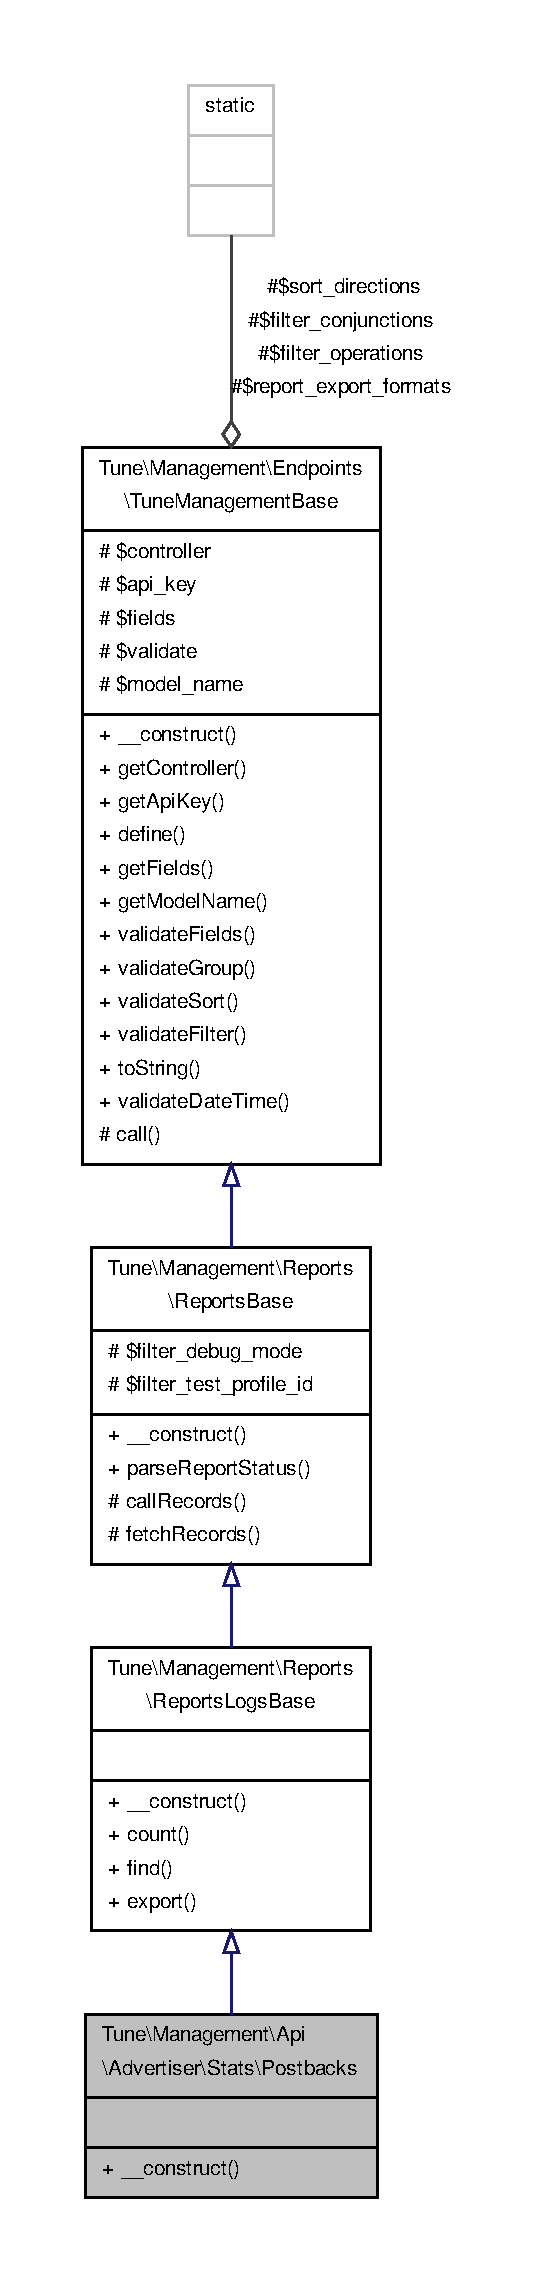
\includegraphics[height=550pt]{classTune_1_1Management_1_1Api_1_1Advertiser_1_1Stats_1_1Postbacks__coll__graph}
\end{center}
\end{figure}
\subsection*{Public Member Functions}
\begin{DoxyCompactItemize}
\item 
\hyperlink{classTune_1_1Management_1_1Api_1_1Advertiser_1_1Stats_1_1Postbacks_ac41b19c897e54ab7b663b53ad9f88b9a}{\-\_\-\-\_\-construct} (\$api\-\_\-key, \$validate=false)
\begin{DoxyCompactList}\small\item\em Constructor. \end{DoxyCompactList}\end{DoxyCompactItemize}
\subsection*{Additional Inherited Members}


\subsection{Detailed Description}
\begin{Desc}
\item[Examples\-: ]\par
\hyperlink{ExamplePostbackUrls_8php-example}{Example\-Postback\-Urls.\-php}.\end{Desc}


Definition at line 48 of file Postbacks.\-php.



\subsection{Constructor \& Destructor Documentation}
\hypertarget{classTune_1_1Management_1_1Api_1_1Advertiser_1_1Stats_1_1Postbacks_ac41b19c897e54ab7b663b53ad9f88b9a}{\index{Tune\-::\-Management\-::\-Api\-::\-Advertiser\-::\-Stats\-::\-Postbacks@{Tune\-::\-Management\-::\-Api\-::\-Advertiser\-::\-Stats\-::\-Postbacks}!\-\_\-\-\_\-construct@{\-\_\-\-\_\-construct}}
\index{\-\_\-\-\_\-construct@{\-\_\-\-\_\-construct}!Tune::Management::Api::Advertiser::Stats::Postbacks@{Tune\-::\-Management\-::\-Api\-::\-Advertiser\-::\-Stats\-::\-Postbacks}}
\subsubsection[{\-\_\-\-\_\-construct}]{\setlength{\rightskip}{0pt plus 5cm}Tune\textbackslash{}\-Management\textbackslash{}\-Api\textbackslash{}\-Advertiser\textbackslash{}\-Stats\textbackslash{}\-Postbacks\-::\-\_\-\-\_\-construct (
\begin{DoxyParamCaption}
\item[{}]{\$api\-\_\-key, }
\item[{}]{\$validate = {\ttfamily false}}
\end{DoxyParamCaption}
)}}\label{classTune_1_1Management_1_1Api_1_1Advertiser_1_1Stats_1_1Postbacks_ac41b19c897e54ab7b663b53ad9f88b9a}


Constructor. 


\begin{DoxyParams}[1]{Parameters}
string & {\em \$api\-\_\-key} & \hyperlink{namespaceTune}{Tune} Mobile\-App\-Tracking A\-P\-I Key. \\
\hline
bool & {\em \$validate} & Validate fields used by actions' parameters. \\
\hline
\end{DoxyParams}


Definition at line 56 of file Postbacks.\-php.


\begin{DoxyCode}
59       \{
60         parent::\_\_construct(
61             \textcolor{stringliteral}{"advertiser/stats/postbacks"},
62             \hyperlink{classTune_1_1Management_1_1Endpoints_1_1TuneManagementBase_ac53649b4bc72055e1d55e53e0b6f244e}{$api\_key},
63             \hyperlink{classTune_1_1Management_1_1Reports_1_1ReportsBase_a6dde408a407042ce3f665e9f16f386b1}{$filter\_debug\_mode} = \textcolor{keyword}{false},
64             \hyperlink{classTune_1_1Management_1_1Reports_1_1ReportsBase_a2a621a3704fdccb98094c2f94bc6180e}{$filter\_test\_profile\_id} = \textcolor{keyword}{true}
65         );
66     \}
\end{DoxyCode}


The documentation for this class was generated from the following file\-:\begin{DoxyCompactItemize}
\item 
lib/\-Tune/\-Management/\-Api/\-Advertiser/\-Stats/\hyperlink{Postbacks_8php}{Postbacks.\-php}\end{DoxyCompactItemize}

\hypertarget{classTune_1_1Management_1_1Service_1_1Proxy}{\section{Tune\textbackslash{}Management\textbackslash{}Service\textbackslash{}Proxy Class Reference}
\label{classTune_1_1Management_1_1Service_1_1Proxy}\index{Tune\textbackslash{}\-Management\textbackslash{}\-Service\textbackslash{}\-Proxy@{Tune\textbackslash{}\-Management\textbackslash{}\-Service\textbackslash{}\-Proxy}}
}


Collaboration diagram for Tune\textbackslash{}Management\textbackslash{}Service\textbackslash{}Proxy\-:
\nopagebreak
\begin{figure}[H]
\begin{center}
\leavevmode
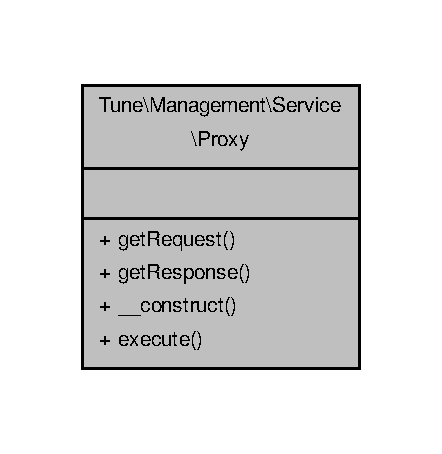
\includegraphics[width=212pt]{classTune_1_1Management_1_1Service_1_1Proxy__coll__graph}
\end{center}
\end{figure}
\subsection*{Public Member Functions}
\begin{DoxyCompactItemize}
\item 
\hyperlink{classTune_1_1Management_1_1Service_1_1Proxy_a61182e1f48960d309fb18492b7b612a6}{get\-Request} ()
\begin{DoxyCompactList}\small\item\em Get request property for this request. \end{DoxyCompactList}\item 
\hyperlink{classTune_1_1Management_1_1Service_1_1Proxy_aad9c18285a8ccb04a24c35909d402719}{get\-Response} ()
\begin{DoxyCompactList}\small\item\em Get response property for this request. \end{DoxyCompactList}\item 
\hyperlink{classTune_1_1Management_1_1Service_1_1Proxy_a9b6e20e49484e5cb55499d0a8b4ac2d3}{\-\_\-\-\_\-construct} (\$request)
\begin{DoxyCompactList}\small\item\em Constructor. \end{DoxyCompactList}\item 
\hyperlink{classTune_1_1Management_1_1Service_1_1Proxy_a680f1cf96a9ecec08d7cb5393938350c}{execute} ()
\begin{DoxyCompactList}\small\item\em Execute to send request to \hyperlink{namespaceTune}{Tune} \hyperlink{namespaceTune_1_1Management}{Management} A\-P\-I, and determine success or failure based upon its service's response. \end{DoxyCompactList}\end{DoxyCompactItemize}


\subsection{Detailed Description}


Definition at line 49 of file Proxy.\-php.



\subsection{Constructor \& Destructor Documentation}
\hypertarget{classTune_1_1Management_1_1Service_1_1Proxy_a9b6e20e49484e5cb55499d0a8b4ac2d3}{\index{Tune\-::\-Management\-::\-Service\-::\-Proxy@{Tune\-::\-Management\-::\-Service\-::\-Proxy}!\-\_\-\-\_\-construct@{\-\_\-\-\_\-construct}}
\index{\-\_\-\-\_\-construct@{\-\_\-\-\_\-construct}!Tune::Management::Service::Proxy@{Tune\-::\-Management\-::\-Service\-::\-Proxy}}
\subsubsection[{\-\_\-\-\_\-construct}]{\setlength{\rightskip}{0pt plus 5cm}Tune\textbackslash{}\-Management\textbackslash{}\-Service\textbackslash{}\-Proxy\-::\-\_\-\-\_\-construct (
\begin{DoxyParamCaption}
\item[{}]{\$request}
\end{DoxyParamCaption}
)}}\label{classTune_1_1Management_1_1Service_1_1Proxy_a9b6e20e49484e5cb55499d0a8b4ac2d3}


Constructor. 


\begin{DoxyParams}[1]{Parameters}
\hyperlink{classTune_1_1Management_1_1Service_1_1Request}{Request} & {\em \$request} & \\
\hline
\end{DoxyParams}


Definition at line 86 of file Proxy.\-php.


\begin{DoxyCode}
87     \{
88         \textcolor{keywordflow}{if} (is\_null($request)) \{
89             \textcolor{keywordflow}{throw} new \(\backslash\)InvalidArgumentException(\textcolor{stringliteral}{"Parameter 'request' is not set."});
90         \}
91 
92         \textcolor{keywordflow}{if} (!is\_a($request, \textcolor{stringliteral}{"\(\backslash\)Tune\(\backslash\)Management\(\backslash\)Service\(\backslash\)Request"})) \{
93             \textcolor{keywordflow}{throw} new \(\backslash\)InvalidArgumentException(
94                 \textcolor{stringliteral}{"Parameter 'request' is not an instance of \(\backslash\)Tune\(\backslash\)Management\(\backslash\)Service\(\backslash\)Request."}
95             );
96         \}
97 
98         \textcolor{keywordflow}{if} (!function\_exists(\textcolor{stringliteral}{'curl\_init'})) \{
99             \textcolor{keywordflow}{throw} new \(\backslash\)RuntimeException(\textcolor{stringliteral}{"PHP extension 'php\_curl' is not installed."});
100         \}
101 
102         $this->request = $request;
103     \}
\end{DoxyCode}


\subsection{Member Function Documentation}
\hypertarget{classTune_1_1Management_1_1Service_1_1Proxy_a680f1cf96a9ecec08d7cb5393938350c}{\index{Tune\-::\-Management\-::\-Service\-::\-Proxy@{Tune\-::\-Management\-::\-Service\-::\-Proxy}!execute@{execute}}
\index{execute@{execute}!Tune::Management::Service::Proxy@{Tune\-::\-Management\-::\-Service\-::\-Proxy}}
\subsubsection[{execute}]{\setlength{\rightskip}{0pt plus 5cm}Tune\textbackslash{}\-Management\textbackslash{}\-Service\textbackslash{}\-Proxy\-::execute (
\begin{DoxyParamCaption}
{}
\end{DoxyParamCaption}
)}}\label{classTune_1_1Management_1_1Service_1_1Proxy_a680f1cf96a9ecec08d7cb5393938350c}


Execute to send request to \hyperlink{namespaceTune}{Tune} \hyperlink{namespaceTune_1_1Management}{Management} A\-P\-I, and determine success or failure based upon its service's response. 

\begin{DoxyReturn}{Returns}
bool 
\end{DoxyReturn}

\begin{DoxyExceptions}{Exceptions}
{\em Tune\-Sdk\-Exception} & \\
\hline
{\em Tune\-Service\-Exception} & \\
\hline
{\em \textbackslash{}\-Exception} & \\
\hline
\end{DoxyExceptions}


Definition at line 114 of file Proxy.\-php.


\begin{DoxyCode}
115     \{
116         \textcolor{keywordflow}{if} (is\_null($this->request)) \{
117             \textcolor{keywordflow}{throw} new \(\backslash\)InvalidArgumentException(\textcolor{stringliteral}{"Parameter 'request' is not set."});
118         \}
119 
120         \textcolor{keywordflow}{if} (!is\_a($this->request, \textcolor{stringliteral}{"\(\backslash\)Tune\(\backslash\)Management\(\backslash\)Service\(\backslash\)Request"})) \{
121             \textcolor{keywordflow}{throw} new \(\backslash\)InvalidArgumentException(
122                 \textcolor{stringliteral}{"Parameter 'request' is not an instance of \(\backslash\)Tune\(\backslash\)Management\(\backslash\)Service\(\backslash\)Request."}
123             );
124         \}
125 
126         $isSuccess = \textcolor{keyword}{false};
127         $response = null;
128         \textcolor{keywordflow}{try} \{
129             $this->uri = $this->request->getUrl();
130             $isSuccess = $this->curlSend();
131         \} \textcolor{keywordflow}{catch} (\(\backslash\)Tune\(\backslash\)Common\(\backslash\)TuneServiceException $ex) \{
132             \textcolor{keywordflow}{throw} $ex;
133         \} \textcolor{keywordflow}{catch} (\(\backslash\)Tune\(\backslash\)Common\(\backslash\)TuneSdkException $ex) \{
134             \textcolor{keywordflow}{throw} $ex;
135         \} \textcolor{keywordflow}{catch} (\hyperlink{classException}{Exception} $ex) \{
136             \textcolor{keywordflow}{throw} new \(\backslash\)Tune\(\backslash\)Common\(\backslash\)TuneSdkException(\textcolor{stringliteral}{"Failed to process request."}, $ex->getCode(), $ex);
137         \}
138         \textcolor{keywordflow}{return} $isSuccess;
139     \}
\end{DoxyCode}
\hypertarget{classTune_1_1Management_1_1Service_1_1Proxy_a61182e1f48960d309fb18492b7b612a6}{\index{Tune\-::\-Management\-::\-Service\-::\-Proxy@{Tune\-::\-Management\-::\-Service\-::\-Proxy}!get\-Request@{get\-Request}}
\index{get\-Request@{get\-Request}!Tune::Management::Service::Proxy@{Tune\-::\-Management\-::\-Service\-::\-Proxy}}
\subsubsection[{get\-Request}]{\setlength{\rightskip}{0pt plus 5cm}Tune\textbackslash{}\-Management\textbackslash{}\-Service\textbackslash{}\-Proxy\-::get\-Request (
\begin{DoxyParamCaption}
{}
\end{DoxyParamCaption}
)}}\label{classTune_1_1Management_1_1Service_1_1Proxy_a61182e1f48960d309fb18492b7b612a6}


Get request property for this request. 

\begin{DoxyReturn}{Returns}
object 
\end{DoxyReturn}


Definition at line 59 of file Proxy.\-php.


\begin{DoxyCode}
60     \{
61         \textcolor{keywordflow}{return} $this->request;
62     \}
\end{DoxyCode}
\hypertarget{classTune_1_1Management_1_1Service_1_1Proxy_aad9c18285a8ccb04a24c35909d402719}{\index{Tune\-::\-Management\-::\-Service\-::\-Proxy@{Tune\-::\-Management\-::\-Service\-::\-Proxy}!get\-Response@{get\-Response}}
\index{get\-Response@{get\-Response}!Tune::Management::Service::Proxy@{Tune\-::\-Management\-::\-Service\-::\-Proxy}}
\subsubsection[{get\-Response}]{\setlength{\rightskip}{0pt plus 5cm}Tune\textbackslash{}\-Management\textbackslash{}\-Service\textbackslash{}\-Proxy\-::get\-Response (
\begin{DoxyParamCaption}
{}
\end{DoxyParamCaption}
)}}\label{classTune_1_1Management_1_1Service_1_1Proxy_aad9c18285a8ccb04a24c35909d402719}


Get response property for this request. 

\begin{DoxyReturn}{Returns}
object 
\end{DoxyReturn}


Definition at line 69 of file Proxy.\-php.


\begin{DoxyCode}
70     \{
71         \textcolor{keywordflow}{return} $this->response;
72     \}
\end{DoxyCode}


The documentation for this class was generated from the following file\-:\begin{DoxyCompactItemize}
\item 
lib/\-Tune/\-Management/\-Service/\hyperlink{Proxy_8php}{Proxy.\-php}\end{DoxyCompactItemize}

\hypertarget{classTune_1_1Management_1_1Service_1_1QueryStringBuilder}{\section{Tune\textbackslash{}Management\textbackslash{}Service\textbackslash{}Query\-String\-Builder Class Reference}
\label{classTune_1_1Management_1_1Service_1_1QueryStringBuilder}\index{Tune\textbackslash{}\-Management\textbackslash{}\-Service\textbackslash{}\-Query\-String\-Builder@{Tune\textbackslash{}\-Management\textbackslash{}\-Service\textbackslash{}\-Query\-String\-Builder}}
}


Collaboration diagram for Tune\textbackslash{}Management\textbackslash{}Service\textbackslash{}Query\-String\-Builder\-:
\nopagebreak
\begin{figure}[H]
\begin{center}
\leavevmode
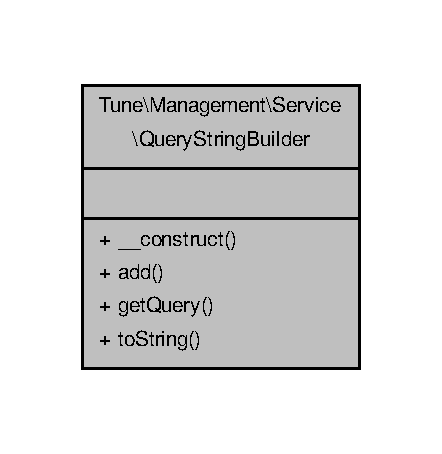
\includegraphics[width=212pt]{classTune_1_1Management_1_1Service_1_1QueryStringBuilder__coll__graph}
\end{center}
\end{figure}
\subsection*{Public Member Functions}
\begin{DoxyCompactItemize}
\item 
\hyperlink{classTune_1_1Management_1_1Service_1_1QueryStringBuilder_ad4e5640aace6fb5d999195d9029bdc88}{\-\_\-\-\_\-construct} (\$name=null, \$value=null)
\begin{DoxyCompactList}\small\item\em Constructor. \end{DoxyCompactList}\item 
\hyperlink{classTune_1_1Management_1_1Service_1_1QueryStringBuilder_ad0f758b9a51e0c2161ef9bc58b583220}{add} (\$name, \$value)
\begin{DoxyCompactList}\small\item\em Add element to query string. \end{DoxyCompactList}\item 
\hyperlink{classTune_1_1Management_1_1Service_1_1QueryStringBuilder_a954b3cb29176e7c64598e8e633dfc0a0}{get\-Query} ()
\begin{DoxyCompactList}\small\item\em Return built query string. \end{DoxyCompactList}\item 
\hyperlink{classTune_1_1Management_1_1Service_1_1QueryStringBuilder_a74ffb882dd3a710fc2fc8cf7f715c5ed}{to\-String} ()
\begin{DoxyCompactList}\small\item\em Custom string representation of object. \end{DoxyCompactList}\end{DoxyCompactItemize}


\subsection{Detailed Description}


Definition at line 49 of file Query\-String\-Builder.\-php.



\subsection{Constructor \& Destructor Documentation}
\hypertarget{classTune_1_1Management_1_1Service_1_1QueryStringBuilder_ad4e5640aace6fb5d999195d9029bdc88}{\index{Tune\-::\-Management\-::\-Service\-::\-Query\-String\-Builder@{Tune\-::\-Management\-::\-Service\-::\-Query\-String\-Builder}!\-\_\-\-\_\-construct@{\-\_\-\-\_\-construct}}
\index{\-\_\-\-\_\-construct@{\-\_\-\-\_\-construct}!Tune::Management::Service::QueryStringBuilder@{Tune\-::\-Management\-::\-Service\-::\-Query\-String\-Builder}}
\subsubsection[{\-\_\-\-\_\-construct}]{\setlength{\rightskip}{0pt plus 5cm}Tune\textbackslash{}\-Management\textbackslash{}\-Service\textbackslash{}\-Query\-String\-Builder\-::\-\_\-\-\_\-construct (
\begin{DoxyParamCaption}
\item[{}]{\$name = {\ttfamily null}, }
\item[{}]{\$value = {\ttfamily null}}
\end{DoxyParamCaption}
)}}\label{classTune_1_1Management_1_1Service_1_1QueryStringBuilder_ad4e5640aace6fb5d999195d9029bdc88}


Constructor. 


\begin{DoxyParams}[1]{Parameters}
string & {\em \$name} & \\
\hline
mixed & {\em \$value} & \\
\hline
\end{DoxyParams}


Definition at line 65 of file Query\-String\-Builder.\-php.


\begin{DoxyCode}
68       \{
69         \textcolor{keywordflow}{if} (is\_string($name) && !empty($name)) \{
70             $this->\hyperlink{classTune_1_1Management_1_1Service_1_1QueryStringBuilder_ad0f758b9a51e0c2161ef9bc58b583220}{add}($name, $value);
71         \}
72     \}
\end{DoxyCode}


Here is the call graph for this function\-:
\nopagebreak
\begin{figure}[H]
\begin{center}
\leavevmode
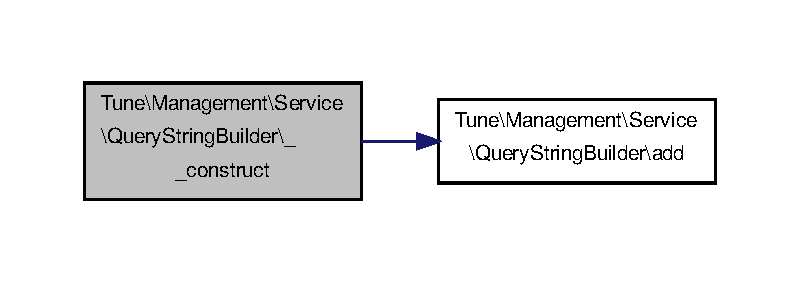
\includegraphics[width=350pt]{classTune_1_1Management_1_1Service_1_1QueryStringBuilder_ad4e5640aace6fb5d999195d9029bdc88_cgraph}
\end{center}
\end{figure}




\subsection{Member Function Documentation}
\hypertarget{classTune_1_1Management_1_1Service_1_1QueryStringBuilder_ad0f758b9a51e0c2161ef9bc58b583220}{\index{Tune\-::\-Management\-::\-Service\-::\-Query\-String\-Builder@{Tune\-::\-Management\-::\-Service\-::\-Query\-String\-Builder}!add@{add}}
\index{add@{add}!Tune::Management::Service::QueryStringBuilder@{Tune\-::\-Management\-::\-Service\-::\-Query\-String\-Builder}}
\subsubsection[{add}]{\setlength{\rightskip}{0pt plus 5cm}Tune\textbackslash{}\-Management\textbackslash{}\-Service\textbackslash{}\-Query\-String\-Builder\-::add (
\begin{DoxyParamCaption}
\item[{}]{\$name, }
\item[{}]{\$value}
\end{DoxyParamCaption}
)}}\label{classTune_1_1Management_1_1Service_1_1QueryStringBuilder_ad0f758b9a51e0c2161ef9bc58b583220}


Add element to query string. 


\begin{DoxyParams}[1]{Parameters}
string & {\em \$name} & \\
\hline
mixed & {\em \$value} & \\
\hline
\end{DoxyParams}


Definition at line 80 of file Query\-String\-Builder.\-php.


\begin{DoxyCode}
81     \{
82 
83         \textcolor{keywordflow}{if} (is\_null($value)) \{
84             \textcolor{keywordflow}{return};
85         \}
86 
87         \textcolor{keywordflow}{if} (!$name || !is\_string($name)) \{
88             \textcolor{keywordflow}{throw} new \(\backslash\)InvalidArgumentException(\textcolor{stringliteral}{"Parameter 'name' must be defined string."});
89         \}
90 
91         $name = trim($name);
92 
93         \textcolor{keywordflow}{if} (empty($name)) \{
94             \textcolor{keywordflow}{throw} new \(\backslash\)InvalidArgumentException(\textcolor{stringliteral}{"Parameter 'name' must be defined string."});
95         \}
96 
97         \textcolor{keywordflow}{if} (is\_string($value)) \{
98             $value = trim($value);
99             \textcolor{keywordflow}{if} (empty($value)) \{
100                 \textcolor{keywordflow}{return};
101             \}
102         \}
103 
104         \textcolor{keywordflow}{try} \{
105             \textcolor{keywordflow}{if} ($name == \textcolor{stringliteral}{"fields"}) \{
106                 $fields\_value = preg\_replace(\textcolor{stringliteral}{'/\(\backslash\)s+/'}, \textcolor{stringliteral}{''}, $value);
107 
108                 $this->encode($name, $fields\_value);
109             \} elseif ($name == \textcolor{stringliteral}{"sort"}) \{
110                 \textcolor{keywordflow}{if} (!is\_array($value)) \{
111                     \textcolor{keywordflow}{throw} new \(\backslash\)InvalidArgumentException(\textcolor{stringliteral}{"Parameter 'sort' value is not a dictionary:
       \{$value\}"});
112                 \}
113 
114                 \textcolor{keywordflow}{foreach} ($value as $sort\_field => $sort\_direction) \{
115                     $sort\_direction = strtoupper($sort\_direction);
116 
117                     \textcolor{keywordflow}{if} ($sort\_direction != \textcolor{stringliteral}{"ASC"} && $sort\_direction != \textcolor{stringliteral}{"DESC"}) \{
118                         \textcolor{keywordflow}{throw} new \(\backslash\)InvalidArgumentException(\textcolor{stringliteral}{"Invalid sort direction: \{$sort\_direction\}."});
119                     \}
120 
121                     $sort\_name = \textcolor{stringliteral}{"sort[\{$sort\_field\}]"};
122                     $sort\_value = $sort\_direction;
123 
124                     $this->encode($sort\_name, $sort\_value);
125                 \}
126             \} elseif ($name == \textcolor{stringliteral}{"filter"}) \{
127                 $filter\_value = preg\_replace(\textcolor{stringliteral}{'/\(\backslash\)s+/'}, \textcolor{charliteral}{' '}, $value);
128 
129                 $this->encode($name, $filter\_value);
130             \} elseif ($name == \textcolor{stringliteral}{"group"}) \{
131                 $group\_value = preg\_replace(\textcolor{stringliteral}{'/\(\backslash\)s+/'}, \textcolor{stringliteral}{''}, $value);
132 
133                 $this->encode($name, $group\_value);
134             \} elseif (is\_bool($value)) \{
135                 $bool\_value = ($value == \textcolor{keyword}{true}) ? \textcolor{stringliteral}{"true"} : \textcolor{stringliteral}{"false"};
136 
137                 $this->encode($name, $bool\_value);
138             \} \textcolor{keywordflow}{else} \{
139                 $this->encode($name, $value);
140             \}
141 
142         \} \textcolor{keywordflow}{catch} (\hyperlink{classException}{Exception} $ex) \{
143             \textcolor{keywordflow}{throw} new \(\backslash\)Tune\(\backslash\)Common\(\backslash\)TuneSdkException(
144                 \textcolor{stringliteral}{"Failed to add query string parameter (\{$name\}, \{$value\})"},
145                 $ex->getCode(),
146                 $ex
147             );
148         \}
149     \}
\end{DoxyCode}


Here is the caller graph for this function\-:
\nopagebreak
\begin{figure}[H]
\begin{center}
\leavevmode
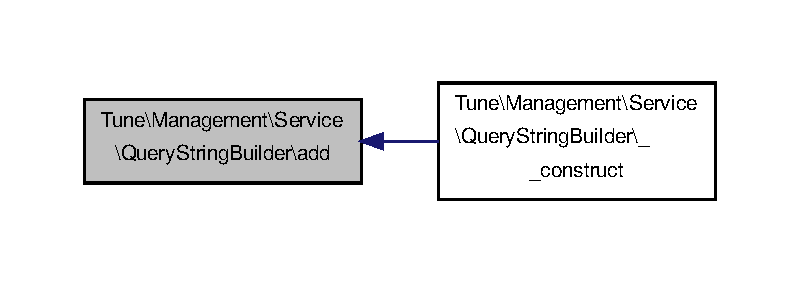
\includegraphics[width=350pt]{classTune_1_1Management_1_1Service_1_1QueryStringBuilder_ad0f758b9a51e0c2161ef9bc58b583220_icgraph}
\end{center}
\end{figure}


\hypertarget{classTune_1_1Management_1_1Service_1_1QueryStringBuilder_a954b3cb29176e7c64598e8e633dfc0a0}{\index{Tune\-::\-Management\-::\-Service\-::\-Query\-String\-Builder@{Tune\-::\-Management\-::\-Service\-::\-Query\-String\-Builder}!get\-Query@{get\-Query}}
\index{get\-Query@{get\-Query}!Tune::Management::Service::QueryStringBuilder@{Tune\-::\-Management\-::\-Service\-::\-Query\-String\-Builder}}
\subsubsection[{get\-Query}]{\setlength{\rightskip}{0pt plus 5cm}Tune\textbackslash{}\-Management\textbackslash{}\-Service\textbackslash{}\-Query\-String\-Builder\-::get\-Query (
\begin{DoxyParamCaption}
{}
\end{DoxyParamCaption}
)}}\label{classTune_1_1Management_1_1Service_1_1QueryStringBuilder_a954b3cb29176e7c64598e8e633dfc0a0}


Return built query string. 

\begin{DoxyReturn}{Returns}
string 
\end{DoxyReturn}


Definition at line 174 of file Query\-String\-Builder.\-php.


\begin{DoxyCode}
175     \{
176         \textcolor{keywordflow}{return} $this->query\_string;
177     \}
\end{DoxyCode}


Here is the caller graph for this function\-:
\nopagebreak
\begin{figure}[H]
\begin{center}
\leavevmode
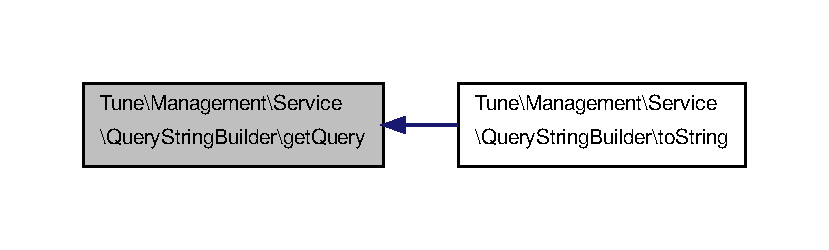
\includegraphics[width=350pt]{classTune_1_1Management_1_1Service_1_1QueryStringBuilder_a954b3cb29176e7c64598e8e633dfc0a0_icgraph}
\end{center}
\end{figure}


\hypertarget{classTune_1_1Management_1_1Service_1_1QueryStringBuilder_a74ffb882dd3a710fc2fc8cf7f715c5ed}{\index{Tune\-::\-Management\-::\-Service\-::\-Query\-String\-Builder@{Tune\-::\-Management\-::\-Service\-::\-Query\-String\-Builder}!to\-String@{to\-String}}
\index{to\-String@{to\-String}!Tune::Management::Service::QueryStringBuilder@{Tune\-::\-Management\-::\-Service\-::\-Query\-String\-Builder}}
\subsubsection[{to\-String}]{\setlength{\rightskip}{0pt plus 5cm}Tune\textbackslash{}\-Management\textbackslash{}\-Service\textbackslash{}\-Query\-String\-Builder\-::to\-String (
\begin{DoxyParamCaption}
{}
\end{DoxyParamCaption}
)}}\label{classTune_1_1Management_1_1Service_1_1QueryStringBuilder_a74ffb882dd3a710fc2fc8cf7f715c5ed}


Custom string representation of object. 

\begin{DoxyReturn}{Returns}
string 
\end{DoxyReturn}


Definition at line 184 of file Query\-String\-Builder.\-php.


\begin{DoxyCode}
185     \{
186         \textcolor{keywordflow}{return} $this->\hyperlink{classTune_1_1Management_1_1Service_1_1QueryStringBuilder_a954b3cb29176e7c64598e8e633dfc0a0}{getQuery}();
187     \}
\end{DoxyCode}


Here is the call graph for this function\-:
\nopagebreak
\begin{figure}[H]
\begin{center}
\leavevmode
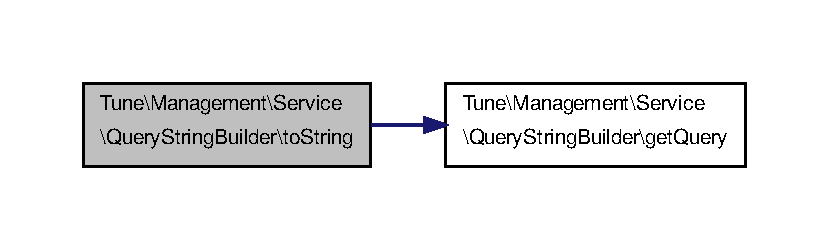
\includegraphics[width=350pt]{classTune_1_1Management_1_1Service_1_1QueryStringBuilder_a74ffb882dd3a710fc2fc8cf7f715c5ed_cgraph}
\end{center}
\end{figure}




The documentation for this class was generated from the following file\-:\begin{DoxyCompactItemize}
\item 
lib/\-Tune/\-Management/\-Service/\hyperlink{QueryStringBuilder_8php}{Query\-String\-Builder.\-php}\end{DoxyCompactItemize}

\hypertarget{classTune_1_1Management_1_1Reports_1_1ReportExportWorker}{\section{Tune\textbackslash{}Management\textbackslash{}Reports\textbackslash{}Report\-Export\-Worker Class Reference}
\label{classTune_1_1Management_1_1Reports_1_1ReportExportWorker}\index{Tune\textbackslash{}\-Management\textbackslash{}\-Reports\textbackslash{}\-Report\-Export\-Worker@{Tune\textbackslash{}\-Management\textbackslash{}\-Reports\textbackslash{}\-Report\-Export\-Worker}}
}


Inheritance diagram for Tune\textbackslash{}Management\textbackslash{}Reports\textbackslash{}Report\-Export\-Worker\-:
\nopagebreak
\begin{figure}[H]
\begin{center}
\leavevmode
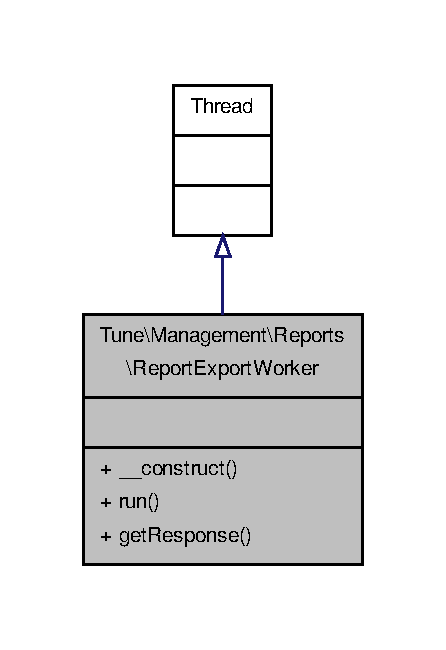
\includegraphics[width=214pt]{classTune_1_1Management_1_1Reports_1_1ReportExportWorker__inherit__graph}
\end{center}
\end{figure}


Collaboration diagram for Tune\textbackslash{}Management\textbackslash{}Reports\textbackslash{}Report\-Export\-Worker\-:
\nopagebreak
\begin{figure}[H]
\begin{center}
\leavevmode
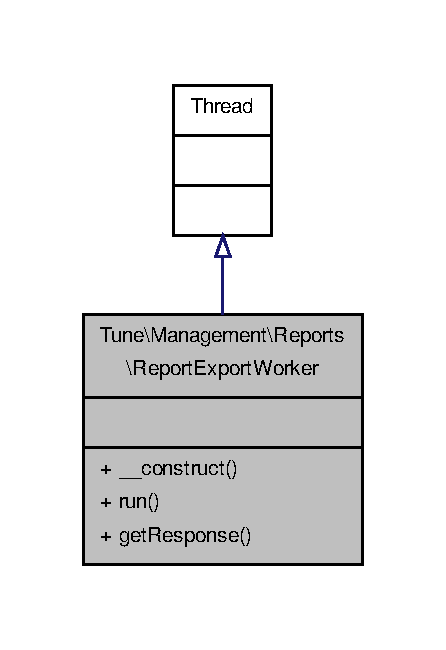
\includegraphics[width=214pt]{classTune_1_1Management_1_1Reports_1_1ReportExportWorker__coll__graph}
\end{center}
\end{figure}
\subsection*{Public Member Functions}
\begin{DoxyCompactItemize}
\item 
\hyperlink{classTune_1_1Management_1_1Reports_1_1ReportExportWorker_aa5311f1c14052f030ab7026e39e45f24}{\-\_\-\-\_\-construct} (\$mod\-\_\-export\-\_\-class, \$mod\-\_\-export\-\_\-function, \$api\-\_\-key, \$job\-\_\-id, \$verbose=false, \$sleep=60)
\begin{DoxyCompactList}\small\item\em Constructor. \end{DoxyCompactList}\item 
\hyperlink{classTune_1_1Management_1_1Reports_1_1ReportExportWorker_af686be7659c034935eca1fd7ef073530}{run} ()
\begin{DoxyCompactList}\small\item\em Poll export status and upon completion gather download U\-R\-L referencing requested report. \end{DoxyCompactList}\item 
\hyperlink{classTune_1_1Management_1_1Reports_1_1ReportExportWorker_a5c573a695b7fa6a660d4e7d9d3c02ff6}{get\-Response} ()
\begin{DoxyCompactList}\small\item\em Property that will hold completed report downloaded from \hyperlink{namespaceTune_1_1Management}{Management} A\-P\-I service. \end{DoxyCompactList}\end{DoxyCompactItemize}


\subsection{Detailed Description}


Definition at line 48 of file Report\-Export\-Worker.\-php.



\subsection{Constructor \& Destructor Documentation}
\hypertarget{classTune_1_1Management_1_1Reports_1_1ReportExportWorker_aa5311f1c14052f030ab7026e39e45f24}{\index{Tune\-::\-Management\-::\-Reports\-::\-Report\-Export\-Worker@{Tune\-::\-Management\-::\-Reports\-::\-Report\-Export\-Worker}!\-\_\-\-\_\-construct@{\-\_\-\-\_\-construct}}
\index{\-\_\-\-\_\-construct@{\-\_\-\-\_\-construct}!Tune::Management::Reports::ReportExportWorker@{Tune\-::\-Management\-::\-Reports\-::\-Report\-Export\-Worker}}
\subsubsection[{\-\_\-\-\_\-construct}]{\setlength{\rightskip}{0pt plus 5cm}Tune\textbackslash{}\-Management\textbackslash{}\-Reports\textbackslash{}\-Report\-Export\-Worker\-::\-\_\-\-\_\-construct (
\begin{DoxyParamCaption}
\item[{}]{\$mod\-\_\-export\-\_\-class, }
\item[{}]{\$mod\-\_\-export\-\_\-function, }
\item[{}]{\$api\-\_\-key, }
\item[{}]{\$job\-\_\-id, }
\item[{}]{\$verbose = {\ttfamily false}, }
\item[{}]{\$sleep = {\ttfamily 60}}
\end{DoxyParamCaption}
)}}\label{classTune_1_1Management_1_1Reports_1_1ReportExportWorker_aa5311f1c14052f030ab7026e39e45f24}


Constructor. 


\begin{DoxyParams}[1]{Parameters}
string & {\em \$mod\-\_\-export\-\_\-class} & Reference class name for worker to perform download status query. \\
\hline
string & {\em \$mod\-\_\-export\-\_\-function} & Reference class function name for worker to perform download status query. \\
\hline
string & {\em \$api\-\_\-key} & Mobile\-App\-Tracking A\-P\-I Key \\
\hline
string & {\em \$job\-\_\-id} & Provided Job Identifier to reference requested report on export queue. \\
\hline
bool & {\em \$verbose} & Debug purposes only to view progress of job on export queue. \\
\hline
int & {\em \$sleep} & Polling delay between querying job status on export queue. \\
\hline
\end{DoxyParams}


Definition at line 87 of file Report\-Export\-Worker.\-php.


\begin{DoxyCode}
94       \{
95         \textcolor{keywordflow}{if} (!is\_string($mod\_export\_class) || empty($mod\_export\_class)) \{
96             \textcolor{keywordflow}{throw} new \(\backslash\)InvalidArgumentException(\textcolor{stringliteral}{"Parameter 'mod\_export\_class' is not defined."});
97         \}
98         \textcolor{keywordflow}{if} (!is\_string($mod\_export\_function) || empty($mod\_export\_function)) \{
99             \textcolor{keywordflow}{throw} new \(\backslash\)InvalidArgumentException(\textcolor{stringliteral}{"Parameter 'mod\_export\_function' is not defined."});
100         \}
101         \textcolor{keywordflow}{if} (!is\_string($api\_key) || empty($api\_key)) \{
102             \textcolor{keywordflow}{throw} new \(\backslash\)InvalidArgumentException(\textcolor{stringliteral}{"Parameter 'api\_key' is not defined."});
103         \}
104         \textcolor{keywordflow}{if} (!is\_string($job\_id) || empty($job\_id)) \{
105             \textcolor{keywordflow}{throw} new \(\backslash\)InvalidArgumentException(\textcolor{stringliteral}{"Parameter 'job\_id' is not defined."});
106         \}
107 
108         $instance = \textcolor{keyword}{new} $mod\_export\_class($api\_key);
109 
110         $this->mod\_export\_class = $mod\_export\_class;
111         $this->mod\_export\_function = $mod\_export\_function;
112 
113         $this->api\_key = $api\_key;
114         $this->job\_id = $job\_id;
115         $this->sleep = $sleep;
116 
117         $this->verbose = $verbose;
118         $this->class\_export = $instance;
119         $this->response = null;
120 
121     \}
\end{DoxyCode}


\subsection{Member Function Documentation}
\hypertarget{classTune_1_1Management_1_1Reports_1_1ReportExportWorker_a5c573a695b7fa6a660d4e7d9d3c02ff6}{\index{Tune\-::\-Management\-::\-Reports\-::\-Report\-Export\-Worker@{Tune\-::\-Management\-::\-Reports\-::\-Report\-Export\-Worker}!get\-Response@{get\-Response}}
\index{get\-Response@{get\-Response}!Tune::Management::Reports::ReportExportWorker@{Tune\-::\-Management\-::\-Reports\-::\-Report\-Export\-Worker}}
\subsubsection[{get\-Response}]{\setlength{\rightskip}{0pt plus 5cm}Tune\textbackslash{}\-Management\textbackslash{}\-Reports\textbackslash{}\-Report\-Export\-Worker\-::get\-Response (
\begin{DoxyParamCaption}
{}
\end{DoxyParamCaption}
)}}\label{classTune_1_1Management_1_1Reports_1_1ReportExportWorker_a5c573a695b7fa6a660d4e7d9d3c02ff6}


Property that will hold completed report downloaded from \hyperlink{namespaceTune_1_1Management}{Management} A\-P\-I service. 

\begin{DoxyReturn}{Returns}
object 
\end{DoxyReturn}


Definition at line 189 of file Report\-Export\-Worker.\-php.


\begin{DoxyCode}
190     \{
191         \textcolor{keywordflow}{return} $this->response;
192     \}
\end{DoxyCode}
\hypertarget{classTune_1_1Management_1_1Reports_1_1ReportExportWorker_af686be7659c034935eca1fd7ef073530}{\index{Tune\-::\-Management\-::\-Reports\-::\-Report\-Export\-Worker@{Tune\-::\-Management\-::\-Reports\-::\-Report\-Export\-Worker}!run@{run}}
\index{run@{run}!Tune::Management::Reports::ReportExportWorker@{Tune\-::\-Management\-::\-Reports\-::\-Report\-Export\-Worker}}
\subsubsection[{run}]{\setlength{\rightskip}{0pt plus 5cm}Tune\textbackslash{}\-Management\textbackslash{}\-Reports\textbackslash{}\-Report\-Export\-Worker\-::run (
\begin{DoxyParamCaption}
{}
\end{DoxyParamCaption}
)}}\label{classTune_1_1Management_1_1Reports_1_1ReportExportWorker_af686be7659c034935eca1fd7ef073530}


Poll export status and upon completion gather download U\-R\-L referencing requested report. 


\begin{DoxyExceptions}{Exceptions}
{\em \textbackslash{}\-Tune\textbackslash{}\-Common\textbackslash{}\-Tune\-Sdk\-Exception} & \\
\hline
{\em \textbackslash{}\-Tune\textbackslash{}\-Common\textbackslash{}\-Tune\-Service\-Exception} & \\
\hline
\end{DoxyExceptions}


Definition at line 129 of file Report\-Export\-Worker.\-php.


\begin{DoxyCode}
130     \{
131         $status = null;
132         $response = null;
133         $attempt = 0;
134 
135         \textcolor{keywordflow}{while} (\textcolor{keyword}{true}) \{
136 
137             $mod\_export\_function = $this->mod\_export\_function;
138             $response = $this->class\_export->$mod\_export\_function($this->job\_id);
139 
140             \textcolor{keywordflow}{if} (is\_null($response)) \{
141                 \textcolor{keywordflow}{throw} \textcolor{keyword}{new} TuneSdkException(\textcolor{stringliteral}{"No response returned from export request."});
142             \}
143 
144             $request\_url = $response->getRequestUrl();
145             $response\_http\_code = $response->getHttpCode();
146 
147             \textcolor{keywordflow}{if} (is\_null($response->getData())) \{
148                 \textcolor{keywordflow}{throw} \textcolor{keyword}{new} TuneSdkException(
149                     \textcolor{stringliteral}{"No response data returned from export. Request URL: '\{$request\_url\}'"}
150                 );
151             \}
152 
153             \textcolor{keywordflow}{if} ($response\_http\_code != 200) \{
154                 \textcolor{keywordflow}{throw} \textcolor{keyword}{new} TuneServiceException(
155                     \textcolor{stringliteral}{"Service failed request: \{$response\_http\_code\}. Request URL: '\{$request\_url\}'"}
156                 );
157             \}
158 
159             $status = $response->getData()[\textcolor{stringliteral}{"status"}];
160             \textcolor{keywordflow}{if} ($status == \textcolor{stringliteral}{"fail"} || $status == \textcolor{stringliteral}{"complete"}) \{
161                 \textcolor{keywordflow}{break};
162             \}
163 
164             $attempt += 1;
165             \textcolor{keywordflow}{if} ($this->verbose) \{
166                 echo \textcolor{stringliteral}{"= attempt: \{$attempt\}, response: "} . print\_r($response, \textcolor{keyword}{true}) . PHP\_EOL;
167             \}
168             sleep($this->sleep);
169         \}
170 
171         \textcolor{keywordflow}{if} ($status != \textcolor{stringliteral}{"complete"}) \{
172             \textcolor{keywordflow}{throw} \textcolor{keyword}{new} TuneServiceException(
173                 \textcolor{stringliteral}{"Export request '\{$status\}':, response: "} . print\_r($response, \textcolor{keyword}{true})
174             );
175         \}
176 
177         \textcolor{keywordflow}{if} ($this->verbose) \{
178             echo \textcolor{stringliteral}{"= attempt: \{$attempt\}, response: "} . print\_r($response, \textcolor{keyword}{true}) . PHP\_EOL;
179         \}
180 
181         $this->response = $response;
182     \}
\end{DoxyCode}


The documentation for this class was generated from the following file\-:\begin{DoxyCompactItemize}
\item 
lib/\-Tune/\-Management/\-Reports/\hyperlink{ReportExportWorker_8php}{Report\-Export\-Worker.\-php}\end{DoxyCompactItemize}

\hypertarget{classTune_1_1Management_1_1Reports_1_1ReportReaderBase}{\section{Tune\textbackslash{}Management\textbackslash{}Reports\textbackslash{}Report\-Reader\-Base Class Reference}
\label{classTune_1_1Management_1_1Reports_1_1ReportReaderBase}\index{Tune\textbackslash{}\-Management\textbackslash{}\-Reports\textbackslash{}\-Report\-Reader\-Base@{Tune\textbackslash{}\-Management\textbackslash{}\-Reports\textbackslash{}\-Report\-Reader\-Base}}
}


Inheritance diagram for Tune\textbackslash{}Management\textbackslash{}Reports\textbackslash{}Report\-Reader\-Base\-:
\nopagebreak
\begin{figure}[H]
\begin{center}
\leavevmode
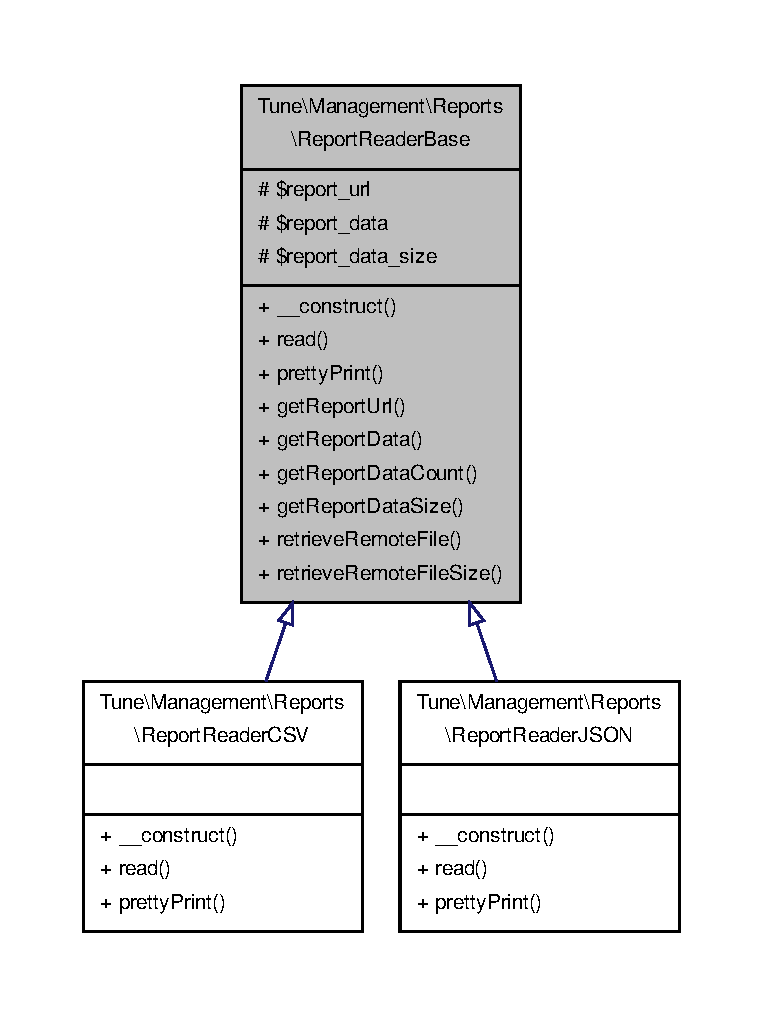
\includegraphics[width=350pt]{classTune_1_1Management_1_1Reports_1_1ReportReaderBase__inherit__graph}
\end{center}
\end{figure}


Collaboration diagram for Tune\textbackslash{}Management\textbackslash{}Reports\textbackslash{}Report\-Reader\-Base\-:
\nopagebreak
\begin{figure}[H]
\begin{center}
\leavevmode
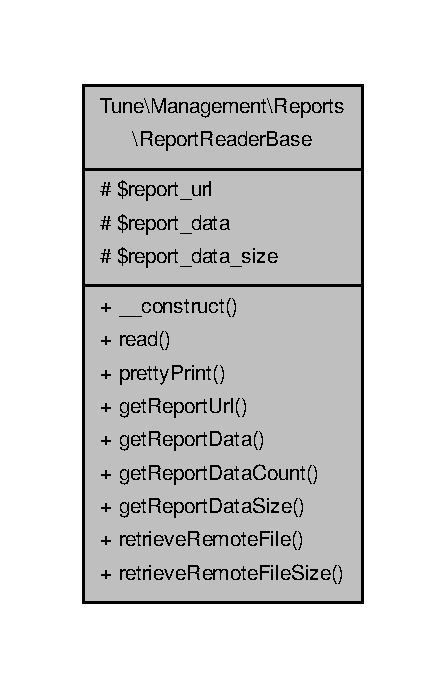
\includegraphics[width=214pt]{classTune_1_1Management_1_1Reports_1_1ReportReaderBase__coll__graph}
\end{center}
\end{figure}
\subsection*{Public Member Functions}
\begin{DoxyCompactItemize}
\item 
\hyperlink{classTune_1_1Management_1_1Reports_1_1ReportReaderBase_a41acf646156b9c6e339f36e13b2b0609}{\-\_\-\-\_\-construct} (\$report\-\_\-url)
\begin{DoxyCompactList}\small\item\em Constructor. \end{DoxyCompactList}\item 
\hyperlink{classTune_1_1Management_1_1Reports_1_1ReportReaderBase_ac6379909340b368795203684ff2cf052}{read} ()
\begin{DoxyCompactList}\small\item\em Using provided report download U\-R\-L, extract contents appropriate to the content's format. \end{DoxyCompactList}\item 
\hyperlink{classTune_1_1Management_1_1Reports_1_1ReportReaderBase_a3f7907396b1f57fe3ca34c41f752a48d}{pretty\-Print} (\$limit=0)
\begin{DoxyCompactList}\small\item\em Using report data pulled from remote file referenced by download U\-R\-L, provide a pretty print of it's contents. \end{DoxyCompactList}\item 
\hyperlink{classTune_1_1Management_1_1Reports_1_1ReportReaderBase_a4a9816979759681b20f8d48a15064847}{get\-Report\-Url} ()
\begin{DoxyCompactList}\small\item\em Report U\-R\-L provided by export status upon completion. \end{DoxyCompactList}\item 
\hyperlink{classTune_1_1Management_1_1Reports_1_1ReportReaderBase_ad725298fd1ca2bd93b4edb16f9eeb7a0}{get\-Report\-Data} ()
\begin{DoxyCompactList}\small\item\em Property providing the contents of exported report. \end{DoxyCompactList}\item 
\hyperlink{classTune_1_1Management_1_1Reports_1_1ReportReaderBase_a2c72cc09cd312685d20b4aed2efd1291}{get\-Report\-Data\-Count} ()
\begin{DoxyCompactList}\small\item\em Property providing the number of rows within contents of exported report. \end{DoxyCompactList}\item 
\hyperlink{classTune_1_1Management_1_1Reports_1_1ReportReaderBase_abd9214311166df72bab2424c2aae273b}{get\-Report\-Data\-Size} ()
\begin{DoxyCompactList}\small\item\em Property providing the number of rows within contents of exported report. \end{DoxyCompactList}\item 
\hyperlink{classTune_1_1Management_1_1Reports_1_1ReportReaderBase_ad624d6972c44e8f45edfaaf13b9cfea6}{retrieve\-Remote\-File} ()
\begin{DoxyCompactList}\small\item\em Reads entire report referenced by exported download U\-R\-L into a string. \end{DoxyCompactList}\item 
\hyperlink{classTune_1_1Management_1_1Reports_1_1ReportReaderBase_aa0e1e91f3872905d85a9d3fa8964a5b8}{retrieve\-Remote\-File\-Size} ()
\begin{DoxyCompactList}\small\item\em Determines size of report referenced by exported download U\-R\-L. \end{DoxyCompactList}\end{DoxyCompactItemize}
\subsection*{Protected Attributes}
\begin{DoxyCompactItemize}
\item 
\hyperlink{classTune_1_1Management_1_1Reports_1_1ReportReaderBase_a90591d693700efd4d05f2b43ac08b552}{\$report\-\_\-url} = null
\begin{DoxyCompactList}\small\item\em Download url of report ready for export. \end{DoxyCompactList}\item 
\hyperlink{classTune_1_1Management_1_1Reports_1_1ReportReaderBase_a4fd2422c90a019e4d1b7d4f4cf2e1541}{\$report\-\_\-data} = null
\begin{DoxyCompactList}\small\item\em Extracted data from report contents. \end{DoxyCompactList}\item 
\hyperlink{classTune_1_1Management_1_1Reports_1_1ReportReaderBase_a41566a442e241ede89e506901b39fb9e}{\$report\-\_\-data\-\_\-size} = null
\begin{DoxyCompactList}\small\item\em Size of extracted data of raw report. \end{DoxyCompactList}\end{DoxyCompactItemize}


\subsection{Detailed Description}


Definition at line 44 of file Report\-Reader\-Base.\-php.



\subsection{Constructor \& Destructor Documentation}
\hypertarget{classTune_1_1Management_1_1Reports_1_1ReportReaderBase_a41acf646156b9c6e339f36e13b2b0609}{\index{Tune\-::\-Management\-::\-Reports\-::\-Report\-Reader\-Base@{Tune\-::\-Management\-::\-Reports\-::\-Report\-Reader\-Base}!\-\_\-\-\_\-construct@{\-\_\-\-\_\-construct}}
\index{\-\_\-\-\_\-construct@{\-\_\-\-\_\-construct}!Tune::Management::Reports::ReportReaderBase@{Tune\-::\-Management\-::\-Reports\-::\-Report\-Reader\-Base}}
\subsubsection[{\-\_\-\-\_\-construct}]{\setlength{\rightskip}{0pt plus 5cm}Tune\textbackslash{}\-Management\textbackslash{}\-Reports\textbackslash{}\-Report\-Reader\-Base\-::\-\_\-\-\_\-construct (
\begin{DoxyParamCaption}
\item[{}]{\$report\-\_\-url}
\end{DoxyParamCaption}
)}}\label{classTune_1_1Management_1_1Reports_1_1ReportReaderBase_a41acf646156b9c6e339f36e13b2b0609}


Constructor. 


\begin{DoxyParams}[1]{Parameters}
string & {\em \$report\-\_\-url} & Download report U\-R\-L of requested report to be exported. \\
\hline
\end{DoxyParams}


Definition at line 69 of file Report\-Reader\-Base.\-php.


\begin{DoxyCode}
70     \{
71         \textcolor{comment}{// report\_url}
72         \textcolor{keywordflow}{if} (!is\_string(\hyperlink{classTune_1_1Management_1_1Reports_1_1ReportReaderBase_a90591d693700efd4d05f2b43ac08b552}{$report\_url}) || empty(\hyperlink{classTune_1_1Management_1_1Reports_1_1ReportReaderBase_a90591d693700efd4d05f2b43ac08b552}{$report\_url})) \{
73             \textcolor{keywordflow}{throw} new \(\backslash\)InvalidArgumentException(\textcolor{stringliteral}{"Parameter 'report\_url' is not defined."});
74         \}
75 
76         $this->report\_url = \hyperlink{classTune_1_1Management_1_1Reports_1_1ReportReaderBase_a90591d693700efd4d05f2b43ac08b552}{$report\_url};
77     \}
\end{DoxyCode}


\subsection{Member Function Documentation}
\hypertarget{classTune_1_1Management_1_1Reports_1_1ReportReaderBase_ad725298fd1ca2bd93b4edb16f9eeb7a0}{\index{Tune\-::\-Management\-::\-Reports\-::\-Report\-Reader\-Base@{Tune\-::\-Management\-::\-Reports\-::\-Report\-Reader\-Base}!get\-Report\-Data@{get\-Report\-Data}}
\index{get\-Report\-Data@{get\-Report\-Data}!Tune::Management::Reports::ReportReaderBase@{Tune\-::\-Management\-::\-Reports\-::\-Report\-Reader\-Base}}
\subsubsection[{get\-Report\-Data}]{\setlength{\rightskip}{0pt plus 5cm}Tune\textbackslash{}\-Management\textbackslash{}\-Reports\textbackslash{}\-Report\-Reader\-Base\-::get\-Report\-Data (
\begin{DoxyParamCaption}
{}
\end{DoxyParamCaption}
)}}\label{classTune_1_1Management_1_1Reports_1_1ReportReaderBase_ad725298fd1ca2bd93b4edb16f9eeb7a0}


Property providing the contents of exported report. 

\begin{DoxyReturn}{Returns}
array 
\end{DoxyReturn}


Definition at line 111 of file Report\-Reader\-Base.\-php.


\begin{DoxyCode}
112     \{
113         \textcolor{keywordflow}{return} \hyperlink{classTune_1_1Management_1_1Reports_1_1ReportReaderBase_a4fd2422c90a019e4d1b7d4f4cf2e1541}{$this->report\_data};
114     \}
\end{DoxyCode}
\hypertarget{classTune_1_1Management_1_1Reports_1_1ReportReaderBase_a2c72cc09cd312685d20b4aed2efd1291}{\index{Tune\-::\-Management\-::\-Reports\-::\-Report\-Reader\-Base@{Tune\-::\-Management\-::\-Reports\-::\-Report\-Reader\-Base}!get\-Report\-Data\-Count@{get\-Report\-Data\-Count}}
\index{get\-Report\-Data\-Count@{get\-Report\-Data\-Count}!Tune::Management::Reports::ReportReaderBase@{Tune\-::\-Management\-::\-Reports\-::\-Report\-Reader\-Base}}
\subsubsection[{get\-Report\-Data\-Count}]{\setlength{\rightskip}{0pt plus 5cm}Tune\textbackslash{}\-Management\textbackslash{}\-Reports\textbackslash{}\-Report\-Reader\-Base\-::get\-Report\-Data\-Count (
\begin{DoxyParamCaption}
{}
\end{DoxyParamCaption}
)}}\label{classTune_1_1Management_1_1Reports_1_1ReportReaderBase_a2c72cc09cd312685d20b4aed2efd1291}


Property providing the number of rows within contents of exported report. 

\begin{DoxyReturn}{Returns}
int Number of rows 
\end{DoxyReturn}


Definition at line 121 of file Report\-Reader\-Base.\-php.


\begin{DoxyCode}
122     \{
123         \textcolor{keywordflow}{return} count($this->report\_data);
124     \}
\end{DoxyCode}
\hypertarget{classTune_1_1Management_1_1Reports_1_1ReportReaderBase_abd9214311166df72bab2424c2aae273b}{\index{Tune\-::\-Management\-::\-Reports\-::\-Report\-Reader\-Base@{Tune\-::\-Management\-::\-Reports\-::\-Report\-Reader\-Base}!get\-Report\-Data\-Size@{get\-Report\-Data\-Size}}
\index{get\-Report\-Data\-Size@{get\-Report\-Data\-Size}!Tune::Management::Reports::ReportReaderBase@{Tune\-::\-Management\-::\-Reports\-::\-Report\-Reader\-Base}}
\subsubsection[{get\-Report\-Data\-Size}]{\setlength{\rightskip}{0pt plus 5cm}Tune\textbackslash{}\-Management\textbackslash{}\-Reports\textbackslash{}\-Report\-Reader\-Base\-::get\-Report\-Data\-Size (
\begin{DoxyParamCaption}
{}
\end{DoxyParamCaption}
)}}\label{classTune_1_1Management_1_1Reports_1_1ReportReaderBase_abd9214311166df72bab2424c2aae273b}


Property providing the number of rows within contents of exported report. 

\begin{DoxyReturn}{Returns}
int Size of exported report data 
\end{DoxyReturn}


Definition at line 131 of file Report\-Reader\-Base.\-php.


\begin{DoxyCode}
132     \{
133         \textcolor{keywordflow}{return} \hyperlink{classTune_1_1Management_1_1Reports_1_1ReportReaderBase_a41566a442e241ede89e506901b39fb9e}{$this->report\_data\_size};
134     \}
\end{DoxyCode}
\hypertarget{classTune_1_1Management_1_1Reports_1_1ReportReaderBase_a4a9816979759681b20f8d48a15064847}{\index{Tune\-::\-Management\-::\-Reports\-::\-Report\-Reader\-Base@{Tune\-::\-Management\-::\-Reports\-::\-Report\-Reader\-Base}!get\-Report\-Url@{get\-Report\-Url}}
\index{get\-Report\-Url@{get\-Report\-Url}!Tune::Management::Reports::ReportReaderBase@{Tune\-::\-Management\-::\-Reports\-::\-Report\-Reader\-Base}}
\subsubsection[{get\-Report\-Url}]{\setlength{\rightskip}{0pt plus 5cm}Tune\textbackslash{}\-Management\textbackslash{}\-Reports\textbackslash{}\-Report\-Reader\-Base\-::get\-Report\-Url (
\begin{DoxyParamCaption}
{}
\end{DoxyParamCaption}
)}}\label{classTune_1_1Management_1_1Reports_1_1ReportReaderBase_a4a9816979759681b20f8d48a15064847}


Report U\-R\-L provided by export status upon completion. 

\begin{DoxyReturn}{Returns}
string 
\end{DoxyReturn}


Definition at line 101 of file Report\-Reader\-Base.\-php.


\begin{DoxyCode}
102     \{
103         \textcolor{keywordflow}{return} \hyperlink{classTune_1_1Management_1_1Reports_1_1ReportReaderBase_a90591d693700efd4d05f2b43ac08b552}{$this->report\_url};
104     \}
\end{DoxyCode}
\hypertarget{classTune_1_1Management_1_1Reports_1_1ReportReaderBase_a3f7907396b1f57fe3ca34c41f752a48d}{\index{Tune\-::\-Management\-::\-Reports\-::\-Report\-Reader\-Base@{Tune\-::\-Management\-::\-Reports\-::\-Report\-Reader\-Base}!pretty\-Print@{pretty\-Print}}
\index{pretty\-Print@{pretty\-Print}!Tune::Management::Reports::ReportReaderBase@{Tune\-::\-Management\-::\-Reports\-::\-Report\-Reader\-Base}}
\subsubsection[{pretty\-Print}]{\setlength{\rightskip}{0pt plus 5cm}Tune\textbackslash{}\-Management\textbackslash{}\-Reports\textbackslash{}\-Report\-Reader\-Base\-::pretty\-Print (
\begin{DoxyParamCaption}
\item[{}]{\$limit = {\ttfamily 0}}
\end{DoxyParamCaption}
)\hspace{0.3cm}{\ttfamily [abstract]}}}\label{classTune_1_1Management_1_1Reports_1_1ReportReaderBase_a3f7907396b1f57fe3ca34c41f752a48d}


Using report data pulled from remote file referenced by download U\-R\-L, provide a pretty print of it's contents. 


\begin{DoxyParams}[1]{Parameters}
int & {\em \$limit} & Limit the number of rows to print.\\
\hline
\end{DoxyParams}
\begin{DoxyReturn}{Returns}
mixed 
\end{DoxyReturn}
\hypertarget{classTune_1_1Management_1_1Reports_1_1ReportReaderBase_ac6379909340b368795203684ff2cf052}{\index{Tune\-::\-Management\-::\-Reports\-::\-Report\-Reader\-Base@{Tune\-::\-Management\-::\-Reports\-::\-Report\-Reader\-Base}!read@{read}}
\index{read@{read}!Tune::Management::Reports::ReportReaderBase@{Tune\-::\-Management\-::\-Reports\-::\-Report\-Reader\-Base}}
\subsubsection[{read}]{\setlength{\rightskip}{0pt plus 5cm}Tune\textbackslash{}\-Management\textbackslash{}\-Reports\textbackslash{}\-Report\-Reader\-Base\-::read (
\begin{DoxyParamCaption}
{}
\end{DoxyParamCaption}
)\hspace{0.3cm}{\ttfamily [abstract]}}}\label{classTune_1_1Management_1_1Reports_1_1ReportReaderBase_ac6379909340b368795203684ff2cf052}


Using provided report download U\-R\-L, extract contents appropriate to the content's format. 

\begin{DoxyReturn}{Returns}
mixed 
\end{DoxyReturn}
\hypertarget{classTune_1_1Management_1_1Reports_1_1ReportReaderBase_ad624d6972c44e8f45edfaaf13b9cfea6}{\index{Tune\-::\-Management\-::\-Reports\-::\-Report\-Reader\-Base@{Tune\-::\-Management\-::\-Reports\-::\-Report\-Reader\-Base}!retrieve\-Remote\-File@{retrieve\-Remote\-File}}
\index{retrieve\-Remote\-File@{retrieve\-Remote\-File}!Tune::Management::Reports::ReportReaderBase@{Tune\-::\-Management\-::\-Reports\-::\-Report\-Reader\-Base}}
\subsubsection[{retrieve\-Remote\-File}]{\setlength{\rightskip}{0pt plus 5cm}Tune\textbackslash{}\-Management\textbackslash{}\-Reports\textbackslash{}\-Report\-Reader\-Base\-::retrieve\-Remote\-File (
\begin{DoxyParamCaption}
{}
\end{DoxyParamCaption}
)}}\label{classTune_1_1Management_1_1Reports_1_1ReportReaderBase_ad624d6972c44e8f45edfaaf13b9cfea6}


Reads entire report referenced by exported download U\-R\-L into a string. 

\begin{DoxyReturn}{Returns}
string The function returns the read data or false on failure. 
\end{DoxyReturn}


Definition at line 141 of file Report\-Reader\-Base.\-php.


\begin{DoxyCode}
142     \{
143         $this->report\_data = file\_get\_contents($this->report\_url);
144     \}
\end{DoxyCode}
\hypertarget{classTune_1_1Management_1_1Reports_1_1ReportReaderBase_aa0e1e91f3872905d85a9d3fa8964a5b8}{\index{Tune\-::\-Management\-::\-Reports\-::\-Report\-Reader\-Base@{Tune\-::\-Management\-::\-Reports\-::\-Report\-Reader\-Base}!retrieve\-Remote\-File\-Size@{retrieve\-Remote\-File\-Size}}
\index{retrieve\-Remote\-File\-Size@{retrieve\-Remote\-File\-Size}!Tune::Management::Reports::ReportReaderBase@{Tune\-::\-Management\-::\-Reports\-::\-Report\-Reader\-Base}}
\subsubsection[{retrieve\-Remote\-File\-Size}]{\setlength{\rightskip}{0pt plus 5cm}Tune\textbackslash{}\-Management\textbackslash{}\-Reports\textbackslash{}\-Report\-Reader\-Base\-::retrieve\-Remote\-File\-Size (
\begin{DoxyParamCaption}
{}
\end{DoxyParamCaption}
)}}\label{classTune_1_1Management_1_1Reports_1_1ReportReaderBase_aa0e1e91f3872905d85a9d3fa8964a5b8}


Determines size of report referenced by exported download U\-R\-L. 

\begin{DoxyReturn}{Returns}
bool$\vert$integer Size of report 
\end{DoxyReturn}


Definition at line 151 of file Report\-Reader\-Base.\-php.


\begin{DoxyCode}
152     \{
153         \textcolor{keyword}{static} $regex = \textcolor{stringliteral}{'/^Content-Length: *+\(\backslash\)K\(\backslash\)d++$/im'};
154         \textcolor{keywordflow}{if} (!$fp = @fopen($this->report\_url, \textcolor{stringliteral}{'rb'})) \{
155             $this->report\_data\_size = -1;
156         \} elseif (isset($http\_response\_header)
157             && preg\_match($regex, implode(\textcolor{stringliteral}{"\(\backslash\)n"}, $http\_response\_header), $matches)
158         ) \{
159             $this->report\_data\_size = (int)$matches[0];
160         \} \textcolor{keywordflow}{else} \{
161             $this->report\_data\_size = strlen(stream\_get\_contents($fp));
162         \}
163     \}
\end{DoxyCode}


Here is the caller graph for this function\-:
\nopagebreak
\begin{figure}[H]
\begin{center}
\leavevmode
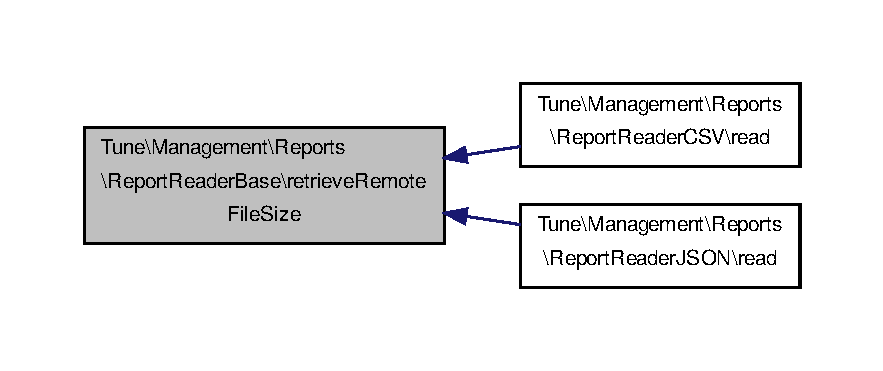
\includegraphics[width=350pt]{classTune_1_1Management_1_1Reports_1_1ReportReaderBase_aa0e1e91f3872905d85a9d3fa8964a5b8_icgraph}
\end{center}
\end{figure}




\subsection{Field Documentation}
\hypertarget{classTune_1_1Management_1_1Reports_1_1ReportReaderBase_a4fd2422c90a019e4d1b7d4f4cf2e1541}{\index{Tune\-::\-Management\-::\-Reports\-::\-Report\-Reader\-Base@{Tune\-::\-Management\-::\-Reports\-::\-Report\-Reader\-Base}!\$report\-\_\-data@{\$report\-\_\-data}}
\index{\$report\-\_\-data@{\$report\-\_\-data}!Tune::Management::Reports::ReportReaderBase@{Tune\-::\-Management\-::\-Reports\-::\-Report\-Reader\-Base}}
\subsubsection[{\$report\-\_\-data}]{\setlength{\rightskip}{0pt plus 5cm}null array Tune\textbackslash{}\-Management\textbackslash{}\-Reports\textbackslash{}\-Report\-Reader\-Base\-::\$report\-\_\-data = null\hspace{0.3cm}{\ttfamily [protected]}}}\label{classTune_1_1Management_1_1Reports_1_1ReportReaderBase_a4fd2422c90a019e4d1b7d4f4cf2e1541}


Extracted data from report contents. 



Definition at line 56 of file Report\-Reader\-Base.\-php.

\hypertarget{classTune_1_1Management_1_1Reports_1_1ReportReaderBase_a41566a442e241ede89e506901b39fb9e}{\index{Tune\-::\-Management\-::\-Reports\-::\-Report\-Reader\-Base@{Tune\-::\-Management\-::\-Reports\-::\-Report\-Reader\-Base}!\$report\-\_\-data\-\_\-size@{\$report\-\_\-data\-\_\-size}}
\index{\$report\-\_\-data\-\_\-size@{\$report\-\_\-data\-\_\-size}!Tune::Management::Reports::ReportReaderBase@{Tune\-::\-Management\-::\-Reports\-::\-Report\-Reader\-Base}}
\subsubsection[{\$report\-\_\-data\-\_\-size}]{\setlength{\rightskip}{0pt plus 5cm}null integer Tune\textbackslash{}\-Management\textbackslash{}\-Reports\textbackslash{}\-Report\-Reader\-Base\-::\$report\-\_\-data\-\_\-size = null\hspace{0.3cm}{\ttfamily [protected]}}}\label{classTune_1_1Management_1_1Reports_1_1ReportReaderBase_a41566a442e241ede89e506901b39fb9e}


Size of extracted data of raw report. 



Definition at line 62 of file Report\-Reader\-Base.\-php.

\hypertarget{classTune_1_1Management_1_1Reports_1_1ReportReaderBase_a90591d693700efd4d05f2b43ac08b552}{\index{Tune\-::\-Management\-::\-Reports\-::\-Report\-Reader\-Base@{Tune\-::\-Management\-::\-Reports\-::\-Report\-Reader\-Base}!\$report\-\_\-url@{\$report\-\_\-url}}
\index{\$report\-\_\-url@{\$report\-\_\-url}!Tune::Management::Reports::ReportReaderBase@{Tune\-::\-Management\-::\-Reports\-::\-Report\-Reader\-Base}}
\subsubsection[{\$report\-\_\-url}]{\setlength{\rightskip}{0pt plus 5cm}null string Tune\textbackslash{}\-Management\textbackslash{}\-Reports\textbackslash{}\-Report\-Reader\-Base\-::\$report\-\_\-url = null\hspace{0.3cm}{\ttfamily [protected]}}}\label{classTune_1_1Management_1_1Reports_1_1ReportReaderBase_a90591d693700efd4d05f2b43ac08b552}


Download url of report ready for export. 



Definition at line 50 of file Report\-Reader\-Base.\-php.



The documentation for this class was generated from the following file\-:\begin{DoxyCompactItemize}
\item 
lib/\-Tune/\-Management/\-Reports/\hyperlink{ReportReaderBase_8php}{Report\-Reader\-Base.\-php}\end{DoxyCompactItemize}

\hypertarget{classTune_1_1Management_1_1Reports_1_1ReportReaderCSV}{\section{Tune\textbackslash{}Management\textbackslash{}Reports\textbackslash{}Report\-Reader\-C\-S\-V Class Reference}
\label{classTune_1_1Management_1_1Reports_1_1ReportReaderCSV}\index{Tune\textbackslash{}\-Management\textbackslash{}\-Reports\textbackslash{}\-Report\-Reader\-C\-S\-V@{Tune\textbackslash{}\-Management\textbackslash{}\-Reports\textbackslash{}\-Report\-Reader\-C\-S\-V}}
}


Inheritance diagram for Tune\textbackslash{}Management\textbackslash{}Reports\textbackslash{}Report\-Reader\-C\-S\-V\-:
\nopagebreak
\begin{figure}[H]
\begin{center}
\leavevmode
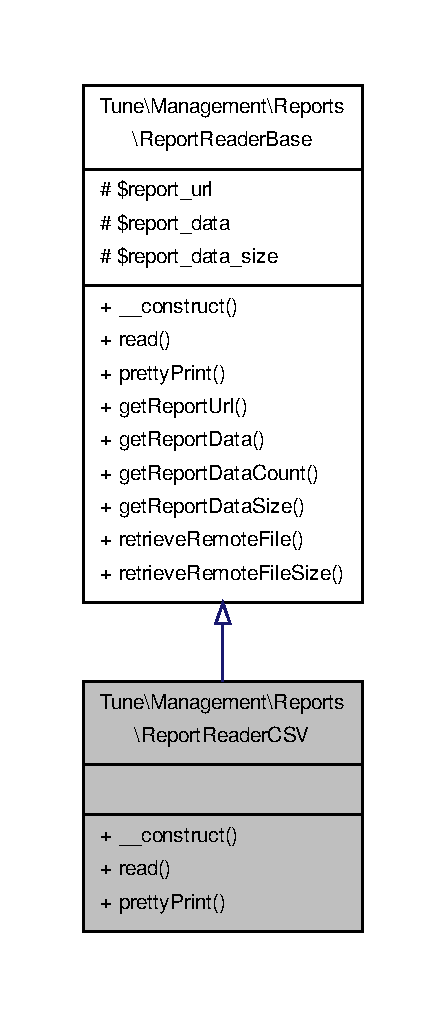
\includegraphics[width=214pt]{classTune_1_1Management_1_1Reports_1_1ReportReaderCSV__inherit__graph}
\end{center}
\end{figure}


Collaboration diagram for Tune\textbackslash{}Management\textbackslash{}Reports\textbackslash{}Report\-Reader\-C\-S\-V\-:
\nopagebreak
\begin{figure}[H]
\begin{center}
\leavevmode
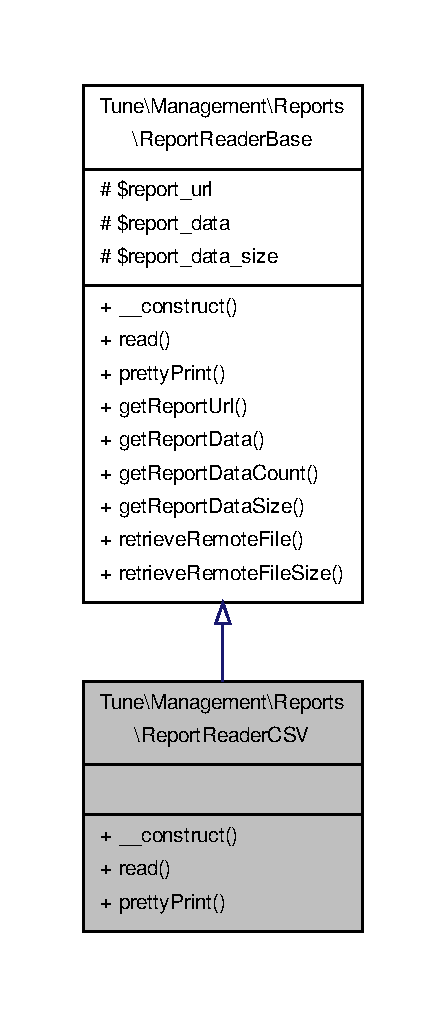
\includegraphics[width=214pt]{classTune_1_1Management_1_1Reports_1_1ReportReaderCSV__coll__graph}
\end{center}
\end{figure}
\subsection*{Public Member Functions}
\begin{DoxyCompactItemize}
\item 
\hyperlink{classTune_1_1Management_1_1Reports_1_1ReportReaderCSV_a2c03ae135945ad6c0a420d6e5df3d227}{\-\_\-\-\_\-construct} (\$report\-\_\-url)
\begin{DoxyCompactList}\small\item\em Constructor. \end{DoxyCompactList}\item 
\hyperlink{classTune_1_1Management_1_1Reports_1_1ReportReaderCSV_adad0aa2d88b5657545134fdf21813af8}{read} ()
\begin{DoxyCompactList}\small\item\em Using provided report download U\-R\-L, extract contents appropriate to the content's format. \end{DoxyCompactList}\item 
\hyperlink{classTune_1_1Management_1_1Reports_1_1ReportReaderCSV_a8f841d3be18e549dbafad31abb889dfa}{pretty\-Print} (\$limit=0)
\begin{DoxyCompactList}\small\item\em Using report data pulled from remote file referenced by download U\-R\-L, provide a pretty print of it's contents. \end{DoxyCompactList}\end{DoxyCompactItemize}
\subsection*{Additional Inherited Members}


\subsection{Detailed Description}


Definition at line 45 of file Report\-Reader\-C\-S\-V.\-php.



\subsection{Constructor \& Destructor Documentation}
\hypertarget{classTune_1_1Management_1_1Reports_1_1ReportReaderCSV_a2c03ae135945ad6c0a420d6e5df3d227}{\index{Tune\-::\-Management\-::\-Reports\-::\-Report\-Reader\-C\-S\-V@{Tune\-::\-Management\-::\-Reports\-::\-Report\-Reader\-C\-S\-V}!\-\_\-\-\_\-construct@{\-\_\-\-\_\-construct}}
\index{\-\_\-\-\_\-construct@{\-\_\-\-\_\-construct}!Tune::Management::Reports::ReportReaderCSV@{Tune\-::\-Management\-::\-Reports\-::\-Report\-Reader\-C\-S\-V}}
\subsubsection[{\-\_\-\-\_\-construct}]{\setlength{\rightskip}{0pt plus 5cm}Tune\textbackslash{}\-Management\textbackslash{}\-Reports\textbackslash{}\-Report\-Reader\-C\-S\-V\-::\-\_\-\-\_\-construct (
\begin{DoxyParamCaption}
\item[{}]{\$report\-\_\-url}
\end{DoxyParamCaption}
)}}\label{classTune_1_1Management_1_1Reports_1_1ReportReaderCSV_a2c03ae135945ad6c0a420d6e5df3d227}


Constructor. 


\begin{DoxyParams}[1]{Parameters}
string & {\em \$report\-\_\-url} & Download report U\-R\-L of requested report to be exported. \\
\hline
\end{DoxyParams}


Definition at line 52 of file Report\-Reader\-C\-S\-V.\-php.


\begin{DoxyCode}
53     \{
54         parent::\_\_construct(\hyperlink{classTune_1_1Management_1_1Reports_1_1ReportReaderBase_a90591d693700efd4d05f2b43ac08b552}{$report\_url});
55     \}
\end{DoxyCode}


\subsection{Member Function Documentation}
\hypertarget{classTune_1_1Management_1_1Reports_1_1ReportReaderCSV_a8f841d3be18e549dbafad31abb889dfa}{\index{Tune\-::\-Management\-::\-Reports\-::\-Report\-Reader\-C\-S\-V@{Tune\-::\-Management\-::\-Reports\-::\-Report\-Reader\-C\-S\-V}!pretty\-Print@{pretty\-Print}}
\index{pretty\-Print@{pretty\-Print}!Tune::Management::Reports::ReportReaderCSV@{Tune\-::\-Management\-::\-Reports\-::\-Report\-Reader\-C\-S\-V}}
\subsubsection[{pretty\-Print}]{\setlength{\rightskip}{0pt plus 5cm}Tune\textbackslash{}\-Management\textbackslash{}\-Reports\textbackslash{}\-Report\-Reader\-C\-S\-V\-::pretty\-Print (
\begin{DoxyParamCaption}
\item[{}]{\$limit = {\ttfamily 0}}
\end{DoxyParamCaption}
)}}\label{classTune_1_1Management_1_1Reports_1_1ReportReaderCSV_a8f841d3be18e549dbafad31abb889dfa}


Using report data pulled from remote file referenced by download U\-R\-L, provide a pretty print of it's contents. 


\begin{DoxyParams}[1]{Parameters}
int & {\em \$limit} & Limit the number of rows to print.\\
\hline
\end{DoxyParams}
\begin{DoxyReturn}{Returns}
mixed 
\end{DoxyReturn}


Definition at line 96 of file Report\-Reader\-C\-S\-V.\-php.


\begin{DoxyCode}
97     \{
98         echo \textcolor{stringliteral}{"Report REPORT\_URL: "} . $this->report\_url . PHP\_EOL;
99         echo \textcolor{stringliteral}{"Report total row count: "} . count($this->report\_data) . PHP\_EOL;
100         echo \textcolor{stringliteral}{"Report data size: "} . count($this->report\_data\_size) . PHP\_EOL;
101 
102         \textcolor{keywordflow}{if} (count($this->report\_data) > 0) \{
103             echo \textcolor{stringliteral}{"------------------"} . PHP\_EOL;
104             $row\_index = 1;
105             \textcolor{keywordflow}{foreach} ($this->report\_data as $row) \{
106                 echo \textcolor{stringliteral}{"\{$row\_index\}. "} . \textcolor{stringliteral}{"'"} . implode(\textcolor{stringliteral}{"','"}, $row) . \textcolor{stringliteral}{"'"} . PHP\_EOL;
107                 $row\_index++;
108                 \textcolor{keywordflow}{if} (($limit > 0) && ($row\_index > $limit)) \{
109                     \textcolor{keywordflow}{break};
110                 \}
111             \}
112             echo \textcolor{stringliteral}{"------------------"} . PHP\_EOL;
113         \}
114     \}
\end{DoxyCode}
\hypertarget{classTune_1_1Management_1_1Reports_1_1ReportReaderCSV_adad0aa2d88b5657545134fdf21813af8}{\index{Tune\-::\-Management\-::\-Reports\-::\-Report\-Reader\-C\-S\-V@{Tune\-::\-Management\-::\-Reports\-::\-Report\-Reader\-C\-S\-V}!read@{read}}
\index{read@{read}!Tune::Management::Reports::ReportReaderCSV@{Tune\-::\-Management\-::\-Reports\-::\-Report\-Reader\-C\-S\-V}}
\subsubsection[{read}]{\setlength{\rightskip}{0pt plus 5cm}Tune\textbackslash{}\-Management\textbackslash{}\-Reports\textbackslash{}\-Report\-Reader\-C\-S\-V\-::read (
\begin{DoxyParamCaption}
{}
\end{DoxyParamCaption}
)}}\label{classTune_1_1Management_1_1Reports_1_1ReportReaderCSV_adad0aa2d88b5657545134fdf21813af8}


Using provided report download U\-R\-L, extract contents appropriate to the content's format. 

\begin{DoxyReturn}{Returns}
bool$\vert$mixed 
\end{DoxyReturn}

\begin{DoxyExceptions}{Exceptions}
{\em \textbackslash{}\-Tune\textbackslash{}\-Common\textbackslash{}\-Tune\-Sdk\-Exception} & \\
\hline
\end{DoxyExceptions}


Definition at line 63 of file Report\-Reader\-C\-S\-V.\-php.


\begin{DoxyCode}
64     \{
65         $success = \textcolor{keyword}{false};
66 
67         \textcolor{keywordflow}{try} \{
68             $this->\hyperlink{classTune_1_1Management_1_1Reports_1_1ReportReaderBase_aa0e1e91f3872905d85a9d3fa8964a5b8}{retrieveRemoteFileSize}();
69 
70             ini\_set(\textcolor{stringliteral}{'memory\_limit'}, \textcolor{stringliteral}{'1024M'}); \textcolor{comment}{// or you could use 1G}
71 
72             $this->report\_data = array();
73 
74             \textcolor{keywordflow}{if} (($handle = fopen($this->report\_url, \textcolor{stringliteral}{"r"})) !== \textcolor{keyword}{false}) \{
75                 \textcolor{keywordflow}{while} (($row\_data = fgetcsv($handle, 1000, \textcolor{stringliteral}{","})) !== \textcolor{keyword}{false}) \{
76                     $this->report\_data[] = $row\_data;
77                 \}
78                 fclose($handle);
79             \}
80 
81             $success = \textcolor{keyword}{true};
82         \} \textcolor{keywordflow}{catch} (\hyperlink{classException}{Exception} $ex) \{
83             \textcolor{keywordflow}{throw} new \(\backslash\)Tune\(\backslash\)Common\(\backslash\)TuneSdkException(\textcolor{stringliteral}{"Failed to process request."}, $ex->getCode(), $ex);
84         \}
85 
86         \textcolor{keywordflow}{return} $success;
87     \}
\end{DoxyCode}


Here is the call graph for this function\-:
\nopagebreak
\begin{figure}[H]
\begin{center}
\leavevmode
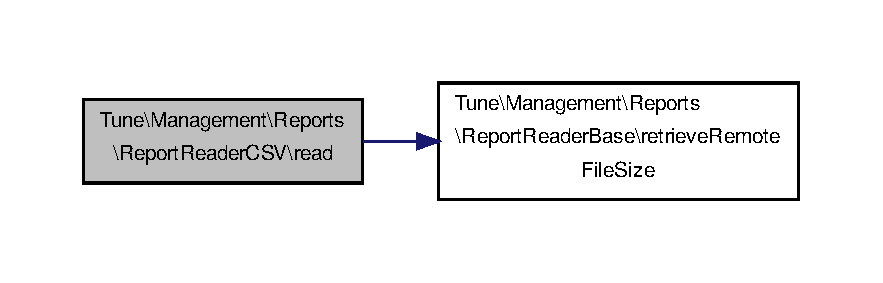
\includegraphics[width=350pt]{classTune_1_1Management_1_1Reports_1_1ReportReaderCSV_adad0aa2d88b5657545134fdf21813af8_cgraph}
\end{center}
\end{figure}




The documentation for this class was generated from the following file\-:\begin{DoxyCompactItemize}
\item 
lib/\-Tune/\-Management/\-Reports/\hyperlink{ReportReaderCSV_8php}{Report\-Reader\-C\-S\-V.\-php}\end{DoxyCompactItemize}

\hypertarget{classTune_1_1Management_1_1Reports_1_1ReportReaderJSON}{\section{Tune\textbackslash{}Management\textbackslash{}Reports\textbackslash{}Report\-Reader\-J\-S\-O\-N Class Reference}
\label{classTune_1_1Management_1_1Reports_1_1ReportReaderJSON}\index{Tune\textbackslash{}\-Management\textbackslash{}\-Reports\textbackslash{}\-Report\-Reader\-J\-S\-O\-N@{Tune\textbackslash{}\-Management\textbackslash{}\-Reports\textbackslash{}\-Report\-Reader\-J\-S\-O\-N}}
}


Inheritance diagram for Tune\textbackslash{}Management\textbackslash{}Reports\textbackslash{}Report\-Reader\-J\-S\-O\-N\-:
\nopagebreak
\begin{figure}[H]
\begin{center}
\leavevmode
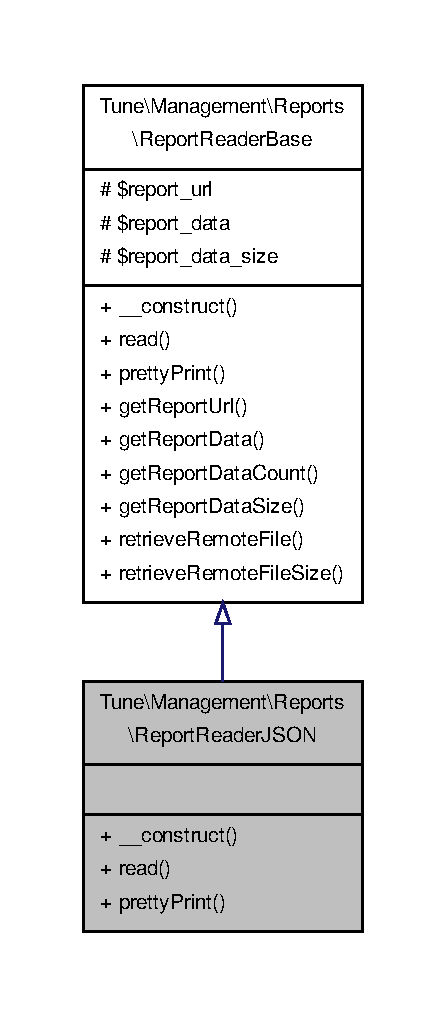
\includegraphics[width=214pt]{classTune_1_1Management_1_1Reports_1_1ReportReaderJSON__inherit__graph}
\end{center}
\end{figure}


Collaboration diagram for Tune\textbackslash{}Management\textbackslash{}Reports\textbackslash{}Report\-Reader\-J\-S\-O\-N\-:
\nopagebreak
\begin{figure}[H]
\begin{center}
\leavevmode
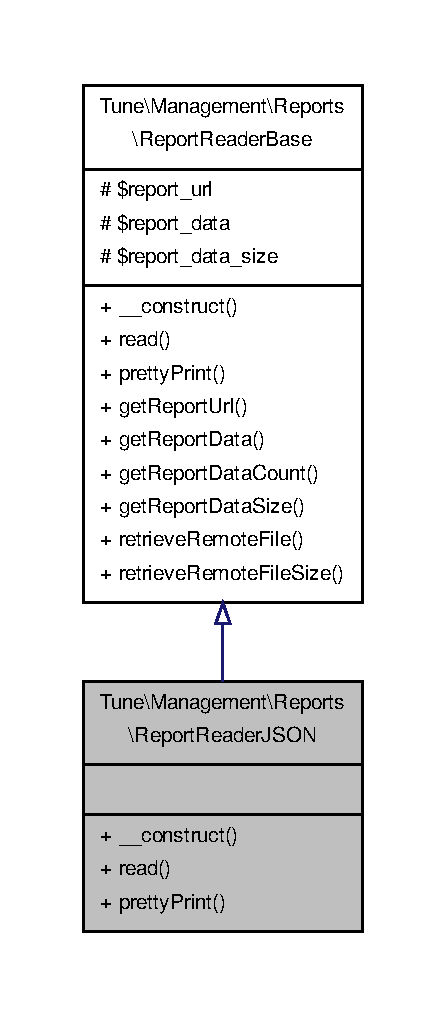
\includegraphics[width=214pt]{classTune_1_1Management_1_1Reports_1_1ReportReaderJSON__coll__graph}
\end{center}
\end{figure}
\subsection*{Public Member Functions}
\begin{DoxyCompactItemize}
\item 
\hyperlink{classTune_1_1Management_1_1Reports_1_1ReportReaderJSON_a8d6da48e523415c0b9ae6ef2d2d8df01}{\-\_\-\-\_\-construct} (\$report\-\_\-url)
\begin{DoxyCompactList}\small\item\em Constructor. \end{DoxyCompactList}\item 
\hyperlink{classTune_1_1Management_1_1Reports_1_1ReportReaderJSON_a2ce2eb7e18962638877a96c06ebed908}{read} ()
\begin{DoxyCompactList}\small\item\em Using provided report download U\-R\-L, extract contents appropriate to the content's format. \end{DoxyCompactList}\item 
\hyperlink{classTune_1_1Management_1_1Reports_1_1ReportReaderJSON_a139f36223334e99aa1e0b55184681741}{pretty\-Print} (\$limit=0)
\begin{DoxyCompactList}\small\item\em Using report data pulled from remote file referenced by download U\-R\-L, provide a pretty print of it's contents. \end{DoxyCompactList}\end{DoxyCompactItemize}
\subsection*{Additional Inherited Members}


\subsection{Detailed Description}


Definition at line 45 of file Report\-Reader\-J\-S\-O\-N.\-php.



\subsection{Constructor \& Destructor Documentation}
\hypertarget{classTune_1_1Management_1_1Reports_1_1ReportReaderJSON_a8d6da48e523415c0b9ae6ef2d2d8df01}{\index{Tune\-::\-Management\-::\-Reports\-::\-Report\-Reader\-J\-S\-O\-N@{Tune\-::\-Management\-::\-Reports\-::\-Report\-Reader\-J\-S\-O\-N}!\-\_\-\-\_\-construct@{\-\_\-\-\_\-construct}}
\index{\-\_\-\-\_\-construct@{\-\_\-\-\_\-construct}!Tune::Management::Reports::ReportReaderJSON@{Tune\-::\-Management\-::\-Reports\-::\-Report\-Reader\-J\-S\-O\-N}}
\subsubsection[{\-\_\-\-\_\-construct}]{\setlength{\rightskip}{0pt plus 5cm}Tune\textbackslash{}\-Management\textbackslash{}\-Reports\textbackslash{}\-Report\-Reader\-J\-S\-O\-N\-::\-\_\-\-\_\-construct (
\begin{DoxyParamCaption}
\item[{}]{\$report\-\_\-url}
\end{DoxyParamCaption}
)}}\label{classTune_1_1Management_1_1Reports_1_1ReportReaderJSON_a8d6da48e523415c0b9ae6ef2d2d8df01}


Constructor. 


\begin{DoxyParams}[1]{Parameters}
string & {\em \$report\-\_\-url} & Download report U\-R\-L of requested report to be exported. \\
\hline
\end{DoxyParams}


Definition at line 52 of file Report\-Reader\-J\-S\-O\-N.\-php.


\begin{DoxyCode}
53     \{
54         parent::\_\_construct(\hyperlink{classTune_1_1Management_1_1Reports_1_1ReportReaderBase_a90591d693700efd4d05f2b43ac08b552}{$report\_url});
55     \}
\end{DoxyCode}


\subsection{Member Function Documentation}
\hypertarget{classTune_1_1Management_1_1Reports_1_1ReportReaderJSON_a139f36223334e99aa1e0b55184681741}{\index{Tune\-::\-Management\-::\-Reports\-::\-Report\-Reader\-J\-S\-O\-N@{Tune\-::\-Management\-::\-Reports\-::\-Report\-Reader\-J\-S\-O\-N}!pretty\-Print@{pretty\-Print}}
\index{pretty\-Print@{pretty\-Print}!Tune::Management::Reports::ReportReaderJSON@{Tune\-::\-Management\-::\-Reports\-::\-Report\-Reader\-J\-S\-O\-N}}
\subsubsection[{pretty\-Print}]{\setlength{\rightskip}{0pt plus 5cm}Tune\textbackslash{}\-Management\textbackslash{}\-Reports\textbackslash{}\-Report\-Reader\-J\-S\-O\-N\-::pretty\-Print (
\begin{DoxyParamCaption}
\item[{}]{\$limit = {\ttfamily 0}}
\end{DoxyParamCaption}
)}}\label{classTune_1_1Management_1_1Reports_1_1ReportReaderJSON_a139f36223334e99aa1e0b55184681741}


Using report data pulled from remote file referenced by download U\-R\-L, provide a pretty print of it's contents. 


\begin{DoxyParams}[1]{Parameters}
int & {\em \$limit} & Limit the number of rows to print.\\
\hline
\end{DoxyParams}
\begin{DoxyReturn}{Returns}
mixed 
\end{DoxyReturn}


Definition at line 91 of file Report\-Reader\-J\-S\-O\-N.\-php.


\begin{DoxyCode}
92     \{
93         echo \textcolor{stringliteral}{"Report REPORT\_URL: "} . $this->report\_url . PHP\_EOL;
94         echo \textcolor{stringliteral}{"Report total row count: "} . count($this->report\_data) . PHP\_EOL;
95         echo \textcolor{stringliteral}{"Report data size: "} . count($this->report\_data\_size) . PHP\_EOL;
96 
97         \textcolor{keywordflow}{if} (count($this->report\_data) > 0) \{
98             echo \textcolor{stringliteral}{"------------------"} . PHP\_EOL;
99             $row\_index = 1;
100             \textcolor{keywordflow}{foreach} ($this->report\_data as $row) \{
101                 $json\_string = json\_encode($row, JSON\_PRETTY\_PRINT);
102                 $json\_row = str\_replace(array(\textcolor{stringliteral}{"\(\backslash\)r"}, \textcolor{stringliteral}{"\(\backslash\)n"}), \textcolor{stringliteral}{" "}, $json\_string);
103                 echo \textcolor{stringliteral}{"\{$row\_index\}. \{$json\_row\}"} . PHP\_EOL;
104                 $row\_index++;
105                 \textcolor{keywordflow}{if} (($limit > 0) && ($row\_index > $limit)) \{
106                     \textcolor{keywordflow}{break};
107                 \}
108             \}
109             echo \textcolor{stringliteral}{"------------------"} . PHP\_EOL;
110         \}
111     \}
\end{DoxyCode}
\hypertarget{classTune_1_1Management_1_1Reports_1_1ReportReaderJSON_a2ce2eb7e18962638877a96c06ebed908}{\index{Tune\-::\-Management\-::\-Reports\-::\-Report\-Reader\-J\-S\-O\-N@{Tune\-::\-Management\-::\-Reports\-::\-Report\-Reader\-J\-S\-O\-N}!read@{read}}
\index{read@{read}!Tune::Management::Reports::ReportReaderJSON@{Tune\-::\-Management\-::\-Reports\-::\-Report\-Reader\-J\-S\-O\-N}}
\subsubsection[{read}]{\setlength{\rightskip}{0pt plus 5cm}Tune\textbackslash{}\-Management\textbackslash{}\-Reports\textbackslash{}\-Report\-Reader\-J\-S\-O\-N\-::read (
\begin{DoxyParamCaption}
{}
\end{DoxyParamCaption}
)}}\label{classTune_1_1Management_1_1Reports_1_1ReportReaderJSON_a2ce2eb7e18962638877a96c06ebed908}


Using provided report download U\-R\-L, extract contents appropriate to the content's format. 

\begin{DoxyReturn}{Returns}
bool$\vert$mixed 
\end{DoxyReturn}

\begin{DoxyExceptions}{Exceptions}
{\em \textbackslash{}\-Tune\textbackslash{}\-Common\textbackslash{}\-Tune\-Sdk\-Exception} & \\
\hline
\end{DoxyExceptions}


Definition at line 63 of file Report\-Reader\-J\-S\-O\-N.\-php.


\begin{DoxyCode}
64     \{
65 
66         $success = \textcolor{keyword}{false};
67 
68         \textcolor{keywordflow}{try} \{
69             $this->\hyperlink{classTune_1_1Management_1_1Reports_1_1ReportReaderBase_aa0e1e91f3872905d85a9d3fa8964a5b8}{retrieveRemoteFileSize}();
70 
71             ini\_set(\textcolor{stringliteral}{'memory\_limit'}, \textcolor{stringliteral}{'1024M'}); \textcolor{comment}{// or you could use 1G}
72 
73             $content=file\_get\_contents($this->report\_url);
74             $this->report\_data=json\_decode($content);
75 
76             $success = \textcolor{keyword}{true};
77         \} \textcolor{keywordflow}{catch} (\hyperlink{classException}{Exception} $ex) \{
78             \textcolor{keywordflow}{throw} new \(\backslash\)Tune\(\backslash\)Common\(\backslash\)TuneSdkException(\textcolor{stringliteral}{"Failed to process request."}, $ex->getCode(), $ex);
79         \}
80 
81         \textcolor{keywordflow}{return} $success;
82     \}
\end{DoxyCode}


Here is the call graph for this function\-:
\nopagebreak
\begin{figure}[H]
\begin{center}
\leavevmode
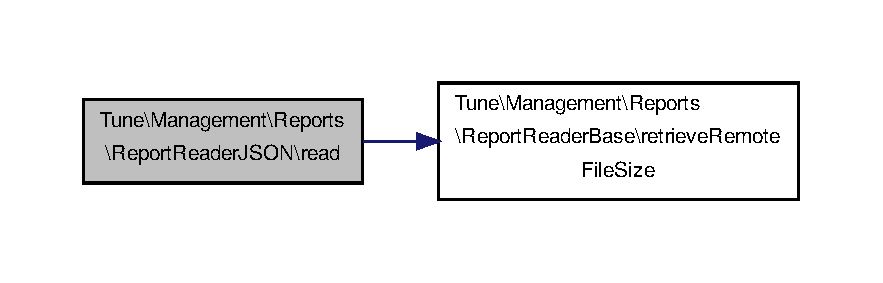
\includegraphics[width=350pt]{classTune_1_1Management_1_1Reports_1_1ReportReaderJSON_a2ce2eb7e18962638877a96c06ebed908_cgraph}
\end{center}
\end{figure}




The documentation for this class was generated from the following file\-:\begin{DoxyCompactItemize}
\item 
lib/\-Tune/\-Management/\-Reports/\hyperlink{ReportReaderJSON_8php}{Report\-Reader\-J\-S\-O\-N.\-php}\end{DoxyCompactItemize}

\hypertarget{classTune_1_1Management_1_1Reports_1_1ReportsActualsBase}{\section{Tune\textbackslash{}Management\textbackslash{}Reports\textbackslash{}Reports\-Actuals\-Base Class Reference}
\label{classTune_1_1Management_1_1Reports_1_1ReportsActualsBase}\index{Tune\textbackslash{}\-Management\textbackslash{}\-Reports\textbackslash{}\-Reports\-Actuals\-Base@{Tune\textbackslash{}\-Management\textbackslash{}\-Reports\textbackslash{}\-Reports\-Actuals\-Base}}
}


Inheritance diagram for Tune\textbackslash{}Management\textbackslash{}Reports\textbackslash{}Reports\-Actuals\-Base\-:
\nopagebreak
\begin{figure}[H]
\begin{center}
\leavevmode
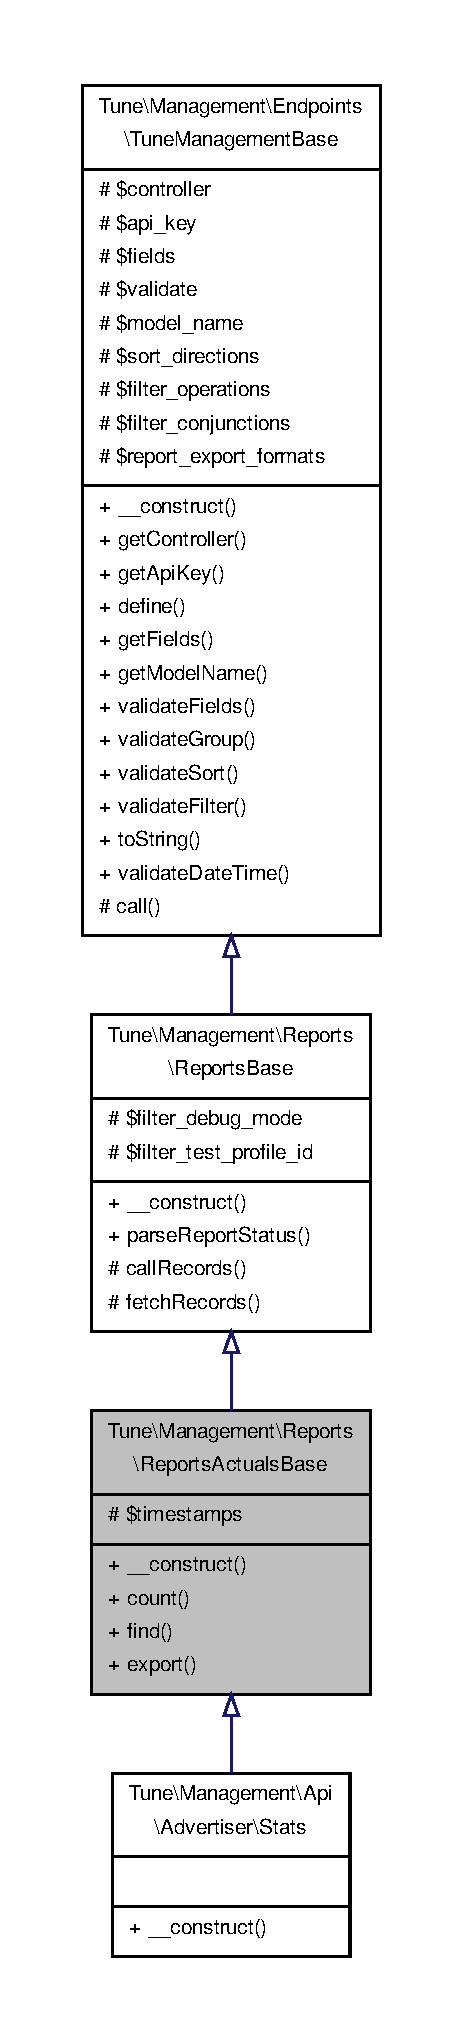
\includegraphics[height=550pt]{classTune_1_1Management_1_1Reports_1_1ReportsActualsBase__inherit__graph}
\end{center}
\end{figure}


Collaboration diagram for Tune\textbackslash{}Management\textbackslash{}Reports\textbackslash{}Reports\-Actuals\-Base\-:
\nopagebreak
\begin{figure}[H]
\begin{center}
\leavevmode
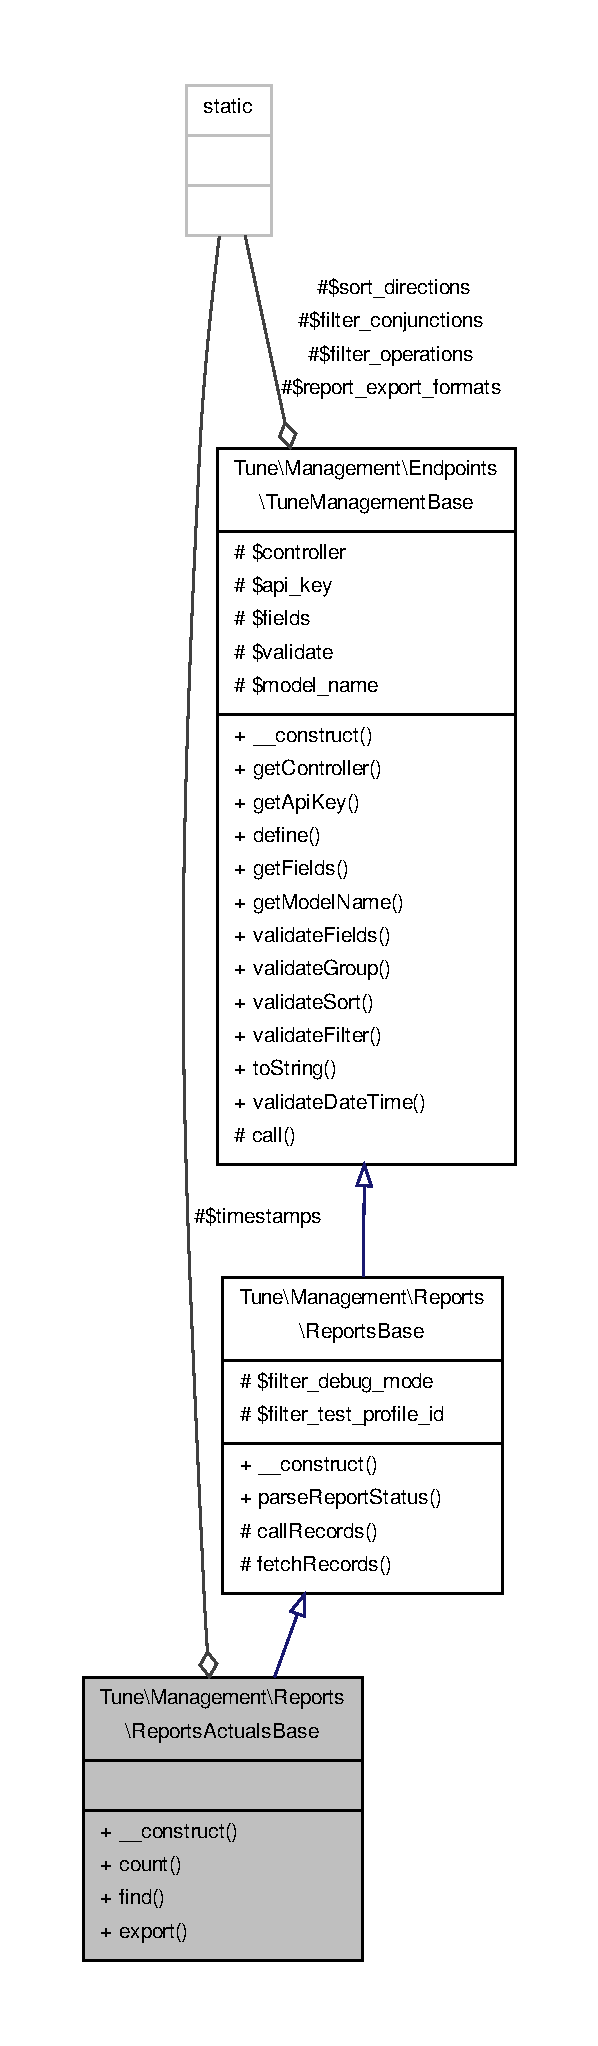
\includegraphics[height=550pt]{classTune_1_1Management_1_1Reports_1_1ReportsActualsBase__coll__graph}
\end{center}
\end{figure}
\subsection*{Public Member Functions}
\begin{DoxyCompactItemize}
\item 
\hyperlink{classTune_1_1Management_1_1Reports_1_1ReportsActualsBase_a7081bd92319b21582ab740fbfc1e9e8c}{\-\_\-\-\_\-construct} (\$controller, \$api\-\_\-key, \$filter\-\_\-debug\-\_\-mode, \$filter\-\_\-test\-\_\-profile\-\_\-id, \$validate=false)
\begin{DoxyCompactList}\small\item\em Constructor. \end{DoxyCompactList}\item 
\hyperlink{classTune_1_1Management_1_1Reports_1_1ReportsActualsBase_a5a8067390a27e402555e878e28e4c54d}{count} (\$start\-\_\-date=null, \$end\-\_\-date=null, \$group=null, \$filter=null, \$response\-\_\-timezone=null)
\begin{DoxyCompactList}\small\item\em Counts all existing records that match filter criteria and returns an array of found model data. \end{DoxyCompactList}\item 
\hyperlink{classTune_1_1Management_1_1Reports_1_1ReportsActualsBase_ace658fea56b4819168acdc7dc2a2fc84}{find} (\$start\-\_\-date=null, \$end\-\_\-date=null, \$group=null, \$filter=null, \$fields=null, \$limit=null, \$page=null, \$sort=null, \$timestamp=null, \$response\-\_\-timezone=null)
\begin{DoxyCompactList}\small\item\em Finds all existing records that match filter criteria and returns an array of found model data. \end{DoxyCompactList}\item 
\hyperlink{classTune_1_1Management_1_1Reports_1_1ReportsActualsBase_aec0b383e43285612314c8ee141c0ebbf}{export} (\$start\-\_\-date=null, \$end\-\_\-date=null, \$group=null, \$filter=null, \$fields=null, \$timestamp=null, \$format=null, \$response\-\_\-timezone=null)
\begin{DoxyCompactList}\small\item\em Places a job into a queue to generate a report that will contain records that match provided filter criteria, and it returns a job identifier to be provided to action /export/download.json to download completed report. \end{DoxyCompactList}\end{DoxyCompactItemize}
\subsection*{Static Protected Attributes}
\begin{DoxyCompactItemize}
\item 
static \hyperlink{classTune_1_1Management_1_1Reports_1_1ReportsActualsBase_a88e430144127cf06384eaaac59111bfc}{\$timestamps}
\end{DoxyCompactItemize}
\subsection*{Additional Inherited Members}


\subsection{Detailed Description}


Definition at line 45 of file Reports\-Actuals\-Base.\-php.



\subsection{Constructor \& Destructor Documentation}
\hypertarget{classTune_1_1Management_1_1Reports_1_1ReportsActualsBase_a7081bd92319b21582ab740fbfc1e9e8c}{\index{Tune\-::\-Management\-::\-Reports\-::\-Reports\-Actuals\-Base@{Tune\-::\-Management\-::\-Reports\-::\-Reports\-Actuals\-Base}!\-\_\-\-\_\-construct@{\-\_\-\-\_\-construct}}
\index{\-\_\-\-\_\-construct@{\-\_\-\-\_\-construct}!Tune::Management::Reports::ReportsActualsBase@{Tune\-::\-Management\-::\-Reports\-::\-Reports\-Actuals\-Base}}
\subsubsection[{\-\_\-\-\_\-construct}]{\setlength{\rightskip}{0pt plus 5cm}Tune\textbackslash{}\-Management\textbackslash{}\-Reports\textbackslash{}\-Reports\-Actuals\-Base\-::\-\_\-\-\_\-construct (
\begin{DoxyParamCaption}
\item[{}]{\$controller, }
\item[{}]{\$api\-\_\-key, }
\item[{}]{\$filter\-\_\-debug\-\_\-mode, }
\item[{}]{\$filter\-\_\-test\-\_\-profile\-\_\-id, }
\item[{}]{\$validate = {\ttfamily false}}
\end{DoxyParamCaption}
)}}\label{classTune_1_1Management_1_1Reports_1_1ReportsActualsBase_a7081bd92319b21582ab740fbfc1e9e8c}


Constructor. 


\begin{DoxyParams}[1]{Parameters}
string & {\em \$controller} & \hyperlink{namespaceTune}{Tune} \hyperlink{namespaceTune_1_1Management}{Management} A\-P\-I endpoint name. \\
\hline
string & {\em \$api\-\_\-key} & \hyperlink{namespaceTune}{Tune} Mobile\-App\-Tracking A\-P\-I Key. \\
\hline
bool & {\em \$filter\-\_\-debug\-\_\-mode} & Remove debug mode information from results. \\
\hline
bool & {\em \$filter\-\_\-test\-\_\-profile\-\_\-id} & Remove test profile information from results. \\
\hline
bool & {\em \$validate} & Validate fields used by actions' parameters. \\
\hline
\end{DoxyParams}


Definition at line 68 of file Reports\-Actuals\-Base.\-php.


\begin{DoxyCode}
74       \{
75         parent::\_\_construct(
76             \hyperlink{classTune_1_1Management_1_1Endpoints_1_1TuneManagementBase_a8a73dbafcc91b04d7f1a7e2aaa9b486a}{$controller},
77             \hyperlink{classTune_1_1Management_1_1Endpoints_1_1TuneManagementBase_ac53649b4bc72055e1d55e53e0b6f244e}{$api\_key},
78             \hyperlink{classTune_1_1Management_1_1Reports_1_1ReportsBase_a6dde408a407042ce3f665e9f16f386b1}{$filter\_debug\_mode},
79             \hyperlink{classTune_1_1Management_1_1Reports_1_1ReportsBase_a2a621a3704fdccb98094c2f94bc6180e}{$filter\_test\_profile\_id},
80             \hyperlink{classTune_1_1Management_1_1Endpoints_1_1TuneManagementBase_a264eed27b0a1c963808fc7eab6da98bc}{$validate}
81         );
82     \}
\end{DoxyCode}


\subsection{Member Function Documentation}
\hypertarget{classTune_1_1Management_1_1Reports_1_1ReportsActualsBase_a5a8067390a27e402555e878e28e4c54d}{\index{Tune\-::\-Management\-::\-Reports\-::\-Reports\-Actuals\-Base@{Tune\-::\-Management\-::\-Reports\-::\-Reports\-Actuals\-Base}!count@{count}}
\index{count@{count}!Tune::Management::Reports::ReportsActualsBase@{Tune\-::\-Management\-::\-Reports\-::\-Reports\-Actuals\-Base}}
\subsubsection[{count}]{\setlength{\rightskip}{0pt plus 5cm}Tune\textbackslash{}\-Management\textbackslash{}\-Reports\textbackslash{}\-Reports\-Actuals\-Base\-::count (
\begin{DoxyParamCaption}
\item[{}]{\$start\-\_\-date = {\ttfamily null}, }
\item[{}]{\$end\-\_\-date = {\ttfamily null}, }
\item[{}]{\$group = {\ttfamily null}, }
\item[{}]{\$filter = {\ttfamily null}, }
\item[{}]{\$response\-\_\-timezone = {\ttfamily null}}
\end{DoxyParamCaption}
)}}\label{classTune_1_1Management_1_1Reports_1_1ReportsActualsBase_a5a8067390a27e402555e878e28e4c54d}


Counts all existing records that match filter criteria and returns an array of found model data. 


\begin{DoxyParams}[1]{Parameters}
string & {\em \$start\-\_\-date} & Y\-Y\-Y\-Y-\/\-M\-M-\/\-D\-D H\-H\-:\-M\-M\-:S\-S \\
\hline
string & {\em \$end\-\_\-date} & Y\-Y\-Y\-Y-\/\-M\-M-\/\-D\-D H\-H\-:\-M\-M\-:S\-S \\
\hline
string & {\em \$group} & Group by one of more field names \\
\hline
string & {\em \$filter} & Filter the results and apply conditions that must be met for records to be included in data. \\
\hline
string & {\em \$response\-\_\-timezone} & Setting expected time for data \\
\hline
\end{DoxyParams}


Definition at line 96 of file Reports\-Actuals\-Base.\-php.


\begin{DoxyCode}
102       \{
103         \textcolor{keywordflow}{if} (!is\_null($start\_date)) \{
104             \hyperlink{classTune_1_1Management_1_1Endpoints_1_1TuneManagementBase_a6a2939da467d84804f36b2e398516b8d}{TuneManagementBase::validateDateTime}(\textcolor{stringliteral}{'start\_date'}, 
      $start\_date);
105         \}
106         \textcolor{keywordflow}{if} (!is\_null($end\_date)) \{
107             \hyperlink{classTune_1_1Management_1_1Endpoints_1_1TuneManagementBase_a6a2939da467d84804f36b2e398516b8d}{TuneManagementBase::validateDateTime}(\textcolor{stringliteral}{'end\_date'}, $end\_date)
      ;
108         \}
109         \textcolor{keywordflow}{if} (!is\_null($group)) \{
110             $filter = $this->\hyperlink{classTune_1_1Management_1_1Endpoints_1_1TuneManagementBase_a54b33f72379846b3c8f8f277bda4bd5f}{validateGroup}($group);
111         \}
112         \textcolor{keywordflow}{if} (!is\_null($filter)) \{
113             $filter = $this->\hyperlink{classTune_1_1Management_1_1Endpoints_1_1TuneManagementBase_a98d644de253513032083a5504fc2f412}{validateFilter}($filter);
114         \}
115 
116         \textcolor{keywordflow}{return} parent::callRecords(
117             $action = \textcolor{stringliteral}{"count"},
118             $query\_string\_dict = array (
119                 \textcolor{stringliteral}{'start\_date'} => $start\_date,
120                 \textcolor{stringliteral}{'end\_date'} => $end\_date,
121                 \textcolor{stringliteral}{'group'} => $group,
122                 \textcolor{stringliteral}{'filter'} => $filter,
123                 \textcolor{stringliteral}{'response\_timezone'} => $response\_timezone
124             )
125         );
126     \}
\end{DoxyCode}


Here is the call graph for this function\-:
\nopagebreak
\begin{figure}[H]
\begin{center}
\leavevmode
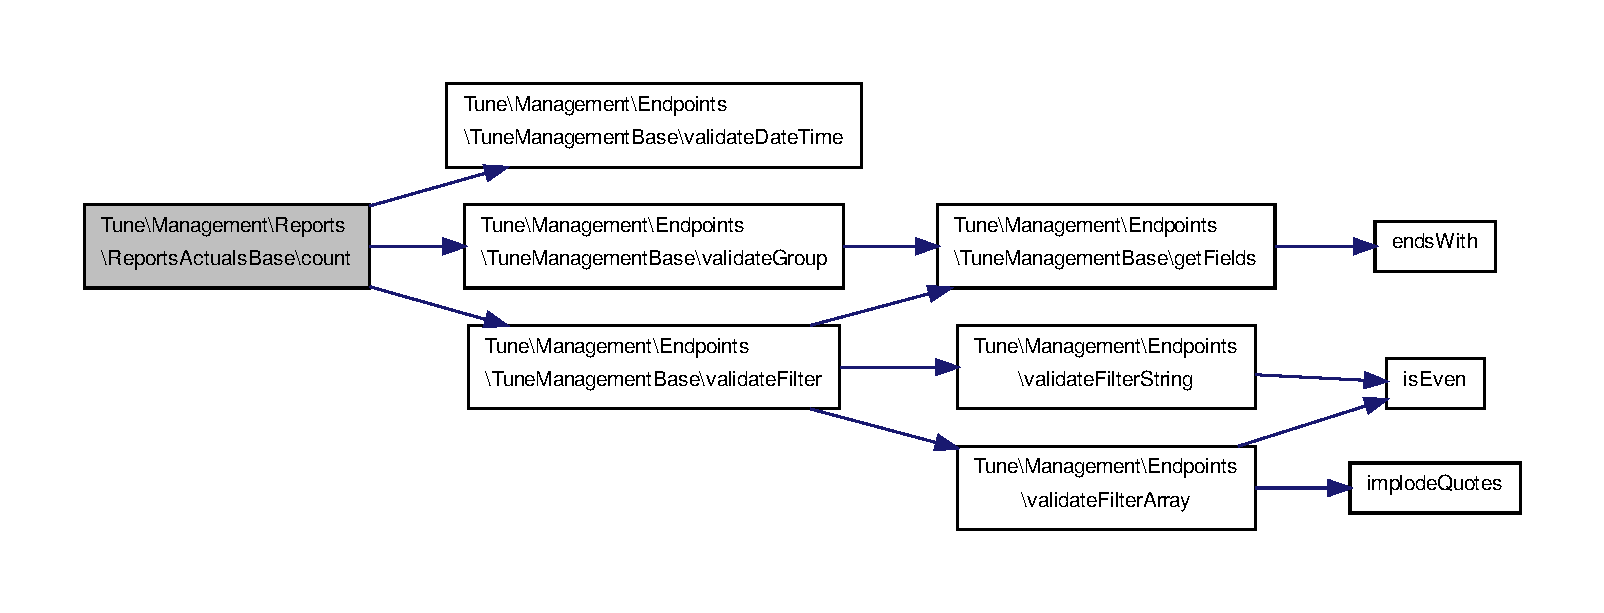
\includegraphics[width=350pt]{classTune_1_1Management_1_1Reports_1_1ReportsActualsBase_a5a8067390a27e402555e878e28e4c54d_cgraph}
\end{center}
\end{figure}


\hypertarget{classTune_1_1Management_1_1Reports_1_1ReportsActualsBase_aec0b383e43285612314c8ee141c0ebbf}{\index{Tune\-::\-Management\-::\-Reports\-::\-Reports\-Actuals\-Base@{Tune\-::\-Management\-::\-Reports\-::\-Reports\-Actuals\-Base}!export@{export}}
\index{export@{export}!Tune::Management::Reports::ReportsActualsBase@{Tune\-::\-Management\-::\-Reports\-::\-Reports\-Actuals\-Base}}
\subsubsection[{export}]{\setlength{\rightskip}{0pt plus 5cm}Tune\textbackslash{}\-Management\textbackslash{}\-Reports\textbackslash{}\-Reports\-Actuals\-Base\-::export (
\begin{DoxyParamCaption}
\item[{}]{\$start\-\_\-date = {\ttfamily null}, }
\item[{}]{\$end\-\_\-date = {\ttfamily null}, }
\item[{}]{\$group = {\ttfamily null}, }
\item[{}]{\$filter = {\ttfamily null}, }
\item[{}]{\$fields = {\ttfamily null}, }
\item[{}]{\$timestamp = {\ttfamily null}, }
\item[{}]{\$format = {\ttfamily null}, }
\item[{}]{\$response\-\_\-timezone = {\ttfamily null}}
\end{DoxyParamCaption}
)}}\label{classTune_1_1Management_1_1Reports_1_1ReportsActualsBase_aec0b383e43285612314c8ee141c0ebbf}


Places a job into a queue to generate a report that will contain records that match provided filter criteria, and it returns a job identifier to be provided to action /export/download.json to download completed report. 


\begin{DoxyParams}[1]{Parameters}
string & {\em \$start\-\_\-date} & Y\-Y\-Y\-Y-\/\-M\-M-\/\-D\-D H\-H\-:\-M\-M\-:S\-S \\
\hline
string & {\em \$end\-\_\-date} & Y\-Y\-Y\-Y-\/\-M\-M-\/\-D\-D H\-H\-:\-M\-M\-:S\-S \\
\hline
string & {\em \$filter} & Filter the results and apply conditions that must be met for records to be included in data. \\
\hline
string & {\em \$fields} & No value returns default fields, \char`\"{}$\ast$\char`\"{} returns all available fields, or provide specific fields. \\
\hline
string & {\em \$timestamp} & Set to breakdown stats by timestamp choices\-: hour, datehour, date, week, month. \\
\hline
string & {\em \$format} & Export format for downloaded report\-: json, csv. \\
\hline
string & {\em \$response\-\_\-timezone} & Setting expected timezone for data. Default is set by account.\\
\hline
\end{DoxyParams}
\begin{DoxyReturn}{Returns}
object 
\end{DoxyReturn}


Definition at line 214 of file Reports\-Actuals\-Base.\-php.


\begin{DoxyCode}
223       \{
224         \textcolor{keywordflow}{if} (!is\_null($start\_date)) \{
225             \hyperlink{classTune_1_1Management_1_1Endpoints_1_1TuneManagementBase_a6a2939da467d84804f36b2e398516b8d}{TuneManagementBase::validateDateTime}(\textcolor{stringliteral}{'start\_date'}, 
      $start\_date);
226         \}
227         \textcolor{keywordflow}{if} (!is\_null($end\_date)) \{
228             \hyperlink{classTune_1_1Management_1_1Endpoints_1_1TuneManagementBase_a6a2939da467d84804f36b2e398516b8d}{TuneManagementBase::validateDateTime}(\textcolor{stringliteral}{'end\_date'}, $end\_date)
      ;
229         \}
230         \textcolor{keywordflow}{if} (!is\_null($group)) \{
231             $filter = $this->\hyperlink{classTune_1_1Management_1_1Endpoints_1_1TuneManagementBase_a54b33f72379846b3c8f8f277bda4bd5f}{validateGroup}($group);
232         \}
233         \textcolor{keywordflow}{if} (!is\_null($filter)) \{
234             $filter = $this->\hyperlink{classTune_1_1Management_1_1Endpoints_1_1TuneManagementBase_a98d644de253513032083a5504fc2f412}{validateFilter}($filter);
235         \}
236 
237         \textcolor{comment}{// timestamp}
238         \textcolor{keywordflow}{if} (is\_string($timestamp) && !in\_array($timestamp, self::$timestamps)) \{
239             \textcolor{keywordflow}{throw} new \(\backslash\)InvalidArgumentException(\textcolor{stringliteral}{"Parameter 'timestamp' is invalid: '\{$timestamp\}'."});
240         \}
241 
242         \textcolor{keywordflow}{if} (!in\_array($format, self::$report\_export\_formats)) \{
243             \textcolor{keywordflow}{throw} new \(\backslash\)InvalidArgumentException(\textcolor{stringliteral}{"Parameter 'format' is invalid: '\{$format\}'."});
244         \}
245 
246         \textcolor{keywordflow}{if} ((\textcolor{stringliteral}{"csv"} == $format) && (is\_null(\hyperlink{classTune_1_1Management_1_1Endpoints_1_1TuneManagementBase_a215be5184c46eee7b2b3febaba85f91b}{$fields}) || empty(\hyperlink{classTune_1_1Management_1_1Endpoints_1_1TuneManagementBase_a215be5184c46eee7b2b3febaba85f91b}{$fields}))) \{
247             \textcolor{keywordflow}{throw} new \(\backslash\)InvalidArgumentException(\textcolor{stringliteral}{"Parameter 'fields' needs to be defined if report format is
       'csv'."});
248         \}
249 
250         \textcolor{keywordflow}{return} parent::callRecords(
251             $action = \textcolor{stringliteral}{"find\_export\_queue"},
252             $query\_string\_dict = array (
253                 \textcolor{stringliteral}{'start\_date'} => $start\_date,
254                 \textcolor{stringliteral}{'end\_date'} => $end\_date,
255                 \textcolor{stringliteral}{'group'} => $group,
256                 \textcolor{stringliteral}{'filter'} => $filter,
257                 \textcolor{stringliteral}{'fields'} => \hyperlink{classTune_1_1Management_1_1Endpoints_1_1TuneManagementBase_a215be5184c46eee7b2b3febaba85f91b}{$fields},
258                 \textcolor{stringliteral}{'timestamp'} => $timestamp,
259                 \textcolor{stringliteral}{'format'} => $format,
260                 \textcolor{stringliteral}{'response\_timezone'} => $response\_timezone
261             )
262         );
263     \}
\end{DoxyCode}


Here is the call graph for this function\-:
\nopagebreak
\begin{figure}[H]
\begin{center}
\leavevmode
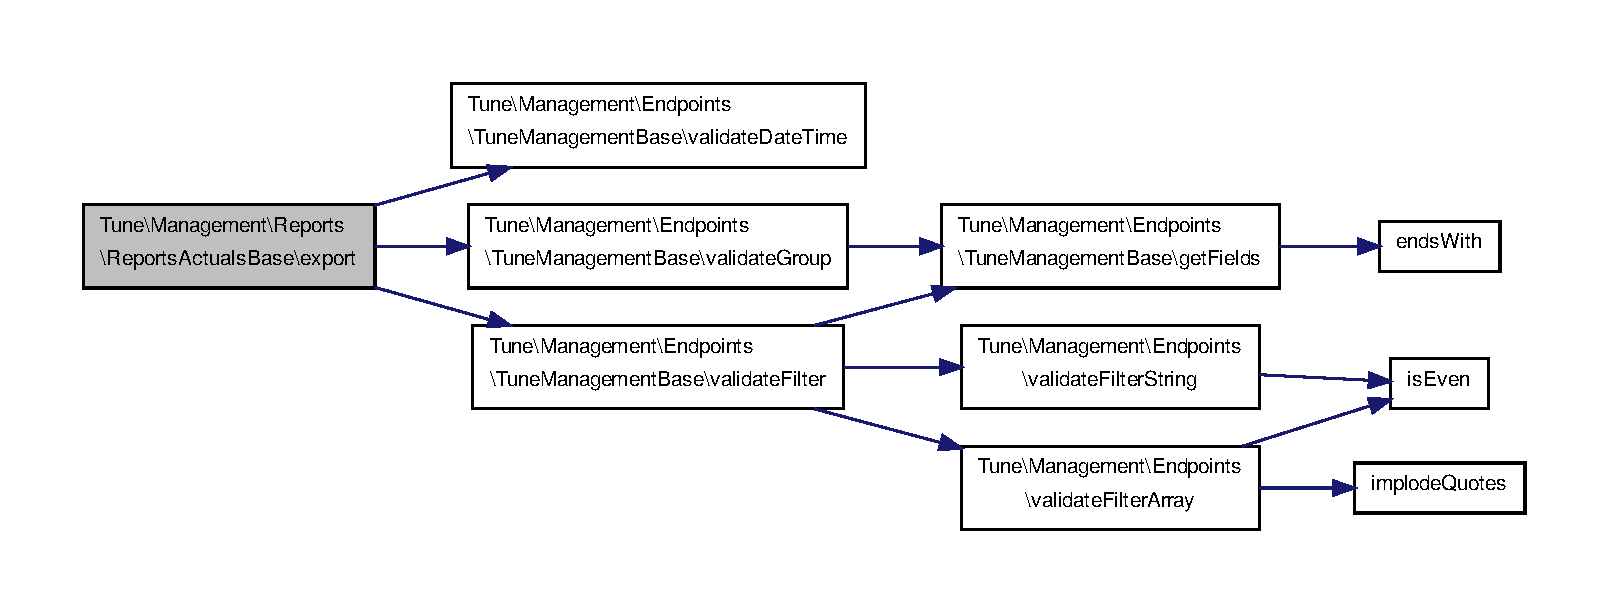
\includegraphics[width=350pt]{classTune_1_1Management_1_1Reports_1_1ReportsActualsBase_aec0b383e43285612314c8ee141c0ebbf_cgraph}
\end{center}
\end{figure}


\hypertarget{classTune_1_1Management_1_1Reports_1_1ReportsActualsBase_ace658fea56b4819168acdc7dc2a2fc84}{\index{Tune\-::\-Management\-::\-Reports\-::\-Reports\-Actuals\-Base@{Tune\-::\-Management\-::\-Reports\-::\-Reports\-Actuals\-Base}!find@{find}}
\index{find@{find}!Tune::Management::Reports::ReportsActualsBase@{Tune\-::\-Management\-::\-Reports\-::\-Reports\-Actuals\-Base}}
\subsubsection[{find}]{\setlength{\rightskip}{0pt plus 5cm}Tune\textbackslash{}\-Management\textbackslash{}\-Reports\textbackslash{}\-Reports\-Actuals\-Base\-::find (
\begin{DoxyParamCaption}
\item[{}]{\$start\-\_\-date = {\ttfamily null}, }
\item[{}]{\$end\-\_\-date = {\ttfamily null}, }
\item[{}]{\$group = {\ttfamily null}, }
\item[{}]{\$filter = {\ttfamily null}, }
\item[{}]{\$fields = {\ttfamily null}, }
\item[{}]{\$limit = {\ttfamily null}, }
\item[{}]{\$page = {\ttfamily null}, }
\item[{}]{\$sort = {\ttfamily null}, }
\item[{}]{\$timestamp = {\ttfamily null}, }
\item[{}]{\$response\-\_\-timezone = {\ttfamily null}}
\end{DoxyParamCaption}
)}}\label{classTune_1_1Management_1_1Reports_1_1ReportsActualsBase_ace658fea56b4819168acdc7dc2a2fc84}


Finds all existing records that match filter criteria and returns an array of found model data. 


\begin{DoxyParams}[1]{Parameters}
string & {\em \$start\-\_\-date} & Y\-Y\-Y\-Y-\/\-M\-M-\/\-D\-D H\-H\-:\-M\-M\-:S\-S \\
\hline
string & {\em \$end\-\_\-date} & Y\-Y\-Y\-Y-\/\-M\-M-\/\-D\-D H\-H\-:\-M\-M\-:S\-S \\
\hline
string & {\em \$filter} & Filter the results and apply conditions that must be met for records to be included in data. \\
\hline
string & {\em \$fields} & No value returns default fields, \char`\"{}$\ast$\char`\"{} returns all available fields, or provide specific fields. \\
\hline
integer & {\em \$limit} & Limit number of results, default 10, 0 shows all. \\
\hline
integer & {\em \$page} & Pagination, default 1. \\
\hline
array & {\em \$sort} & Sort by field name, A\-S\-C (default) or D\-E\-S\-C \\
\hline
string & {\em \$timestamp} & Set to breakdown stats by timestamp choices\-: hour, datehour, date, week, month. \\
\hline
string & {\em \$response\-\_\-timezone} & Setting expected timezone for data. Default is set by account.\\
\hline
\end{DoxyParams}
\begin{DoxyReturn}{Returns}
object 
\end{DoxyReturn}


Definition at line 146 of file Reports\-Actuals\-Base.\-php.


\begin{DoxyCode}
157       \{
158         \textcolor{keywordflow}{if} (!is\_null($start\_date)) \{
159             \hyperlink{classTune_1_1Management_1_1Endpoints_1_1TuneManagementBase_a6a2939da467d84804f36b2e398516b8d}{TuneManagementBase::validateDateTime}(\textcolor{stringliteral}{'start\_date'}, 
      $start\_date);
160         \}
161         \textcolor{keywordflow}{if} (!is\_null($end\_date)) \{
162             \hyperlink{classTune_1_1Management_1_1Endpoints_1_1TuneManagementBase_a6a2939da467d84804f36b2e398516b8d}{TuneManagementBase::validateDateTime}(\textcolor{stringliteral}{'end\_date'}, $end\_date)
      ;
163         \}
164         \textcolor{keywordflow}{if} (!is\_null($group)) \{
165             $filter = $this->\hyperlink{classTune_1_1Management_1_1Endpoints_1_1TuneManagementBase_a54b33f72379846b3c8f8f277bda4bd5f}{validateGroup}($group);
166         \}
167         \textcolor{keywordflow}{if} (!is\_null($filter)) \{
168             $filter = $this->\hyperlink{classTune_1_1Management_1_1Endpoints_1_1TuneManagementBase_a98d644de253513032083a5504fc2f412}{validateFilter}($filter);
169         \}
170         \textcolor{keywordflow}{if} (!is\_null($sort)) \{
171             $sort = $this->\hyperlink{classTune_1_1Management_1_1Endpoints_1_1TuneManagementBase_aa81ef05c1abaf189a0fedb49af9df1bd}{validateSort}($sort);
172         \}
173 
174         \textcolor{comment}{// timestamp}
175         \textcolor{keywordflow}{if} (is\_string($timestamp) && !in\_array($timestamp, self::$timestamps)) \{
176             \textcolor{keywordflow}{throw} new \(\backslash\)InvalidArgumentException(\textcolor{stringliteral}{"Parameter 'timestamp' is invalid: '\{$timestamp\}'."});
177         \}
178 
179         \textcolor{keywordflow}{return} parent::callRecords(
180             $action = \textcolor{stringliteral}{"find"},
181             $query\_string\_dict = array (
182                 \textcolor{stringliteral}{'start\_date'} => $start\_date,
183                 \textcolor{stringliteral}{'end\_date'} => $end\_date,
184                 \textcolor{stringliteral}{'group'} => $group,
185                 \textcolor{stringliteral}{'filter'} => $filter,
186                 \textcolor{stringliteral}{'fields'} => \hyperlink{classTune_1_1Management_1_1Endpoints_1_1TuneManagementBase_a215be5184c46eee7b2b3febaba85f91b}{$fields},
187                 \textcolor{stringliteral}{'limit'} => $limit,
188                 \textcolor{stringliteral}{'page'} => $page,
189                 \textcolor{stringliteral}{'sort'} => $sort,
190                 \textcolor{stringliteral}{'timestamp'} => $timestamp,
191                 \textcolor{stringliteral}{'response\_timezone'} => $response\_timezone
192             )
193         );
194     \}
\end{DoxyCode}


Here is the call graph for this function\-:
\nopagebreak
\begin{figure}[H]
\begin{center}
\leavevmode
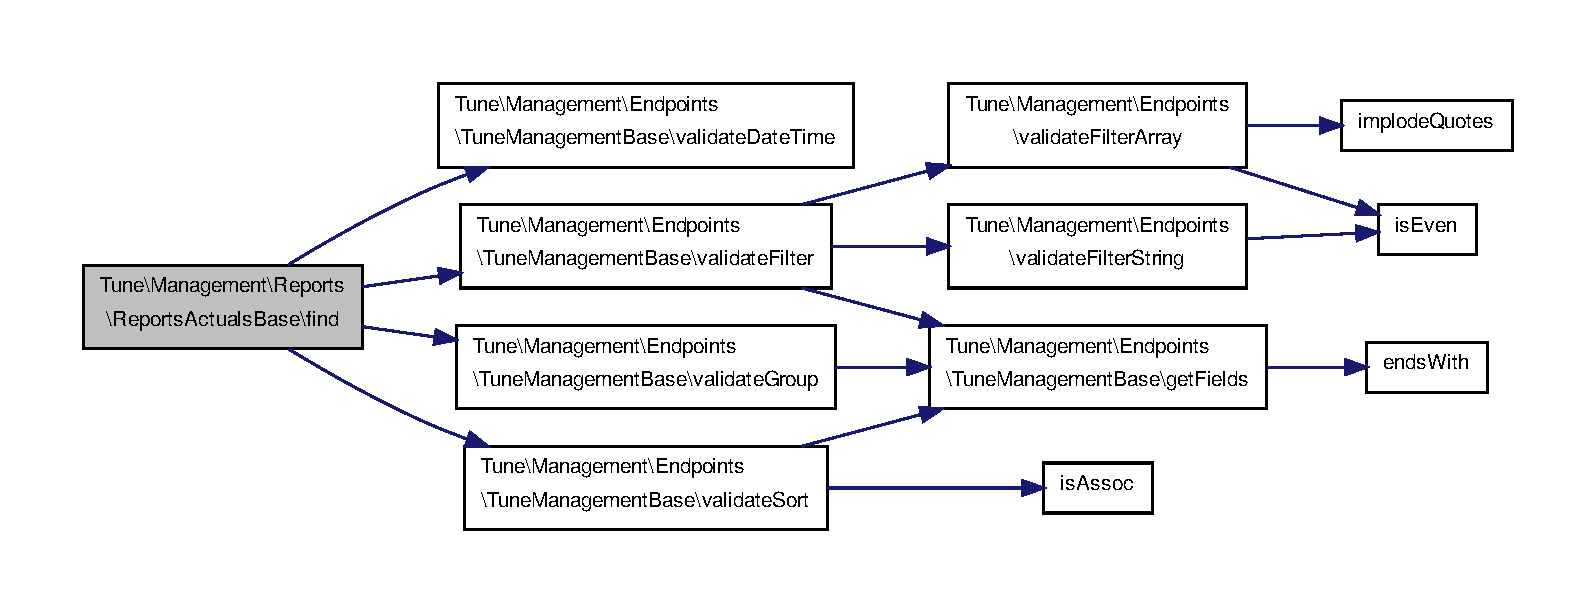
\includegraphics[width=350pt]{classTune_1_1Management_1_1Reports_1_1ReportsActualsBase_ace658fea56b4819168acdc7dc2a2fc84_cgraph}
\end{center}
\end{figure}




\subsection{Field Documentation}
\hypertarget{classTune_1_1Management_1_1Reports_1_1ReportsActualsBase_a88e430144127cf06384eaaac59111bfc}{\index{Tune\-::\-Management\-::\-Reports\-::\-Reports\-Actuals\-Base@{Tune\-::\-Management\-::\-Reports\-::\-Reports\-Actuals\-Base}!\$timestamps@{\$timestamps}}
\index{\$timestamps@{\$timestamps}!Tune::Management::Reports::ReportsActualsBase@{Tune\-::\-Management\-::\-Reports\-::\-Reports\-Actuals\-Base}}
\subsubsection[{\$timestamps}]{\setlength{\rightskip}{0pt plus 5cm}Tune\textbackslash{}\-Management\textbackslash{}\-Reports\textbackslash{}\-Reports\-Actuals\-Base\-::\$timestamps\hspace{0.3cm}{\ttfamily [static]}, {\ttfamily [protected]}}}\label{classTune_1_1Management_1_1Reports_1_1ReportsActualsBase_a88e430144127cf06384eaaac59111bfc}
{\bfseries Initial value\-:}
\begin{DoxyCode}
= array(
            \textcolor{stringliteral}{"hour"},
            \textcolor{stringliteral}{"datehour"},
            \textcolor{stringliteral}{"date"},
            \textcolor{stringliteral}{"week"},
            \textcolor{stringliteral}{"month"}
        )
\end{DoxyCode}


Definition at line 51 of file Reports\-Actuals\-Base.\-php.



The documentation for this class was generated from the following file\-:\begin{DoxyCompactItemize}
\item 
lib/\-Tune/\-Management/\-Reports/\hyperlink{ReportsActualsBase_8php}{Reports\-Actuals\-Base.\-php}\end{DoxyCompactItemize}

\hypertarget{classTune_1_1Management_1_1Reports_1_1ReportsBase}{\section{Tune\textbackslash{}Management\textbackslash{}Reports\textbackslash{}Reports\-Base Class Reference}
\label{classTune_1_1Management_1_1Reports_1_1ReportsBase}\index{Tune\textbackslash{}\-Management\textbackslash{}\-Reports\textbackslash{}\-Reports\-Base@{Tune\textbackslash{}\-Management\textbackslash{}\-Reports\textbackslash{}\-Reports\-Base}}
}


Inheritance diagram for Tune\textbackslash{}Management\textbackslash{}Reports\textbackslash{}Reports\-Base\-:
\nopagebreak
\begin{figure}[H]
\begin{center}
\leavevmode
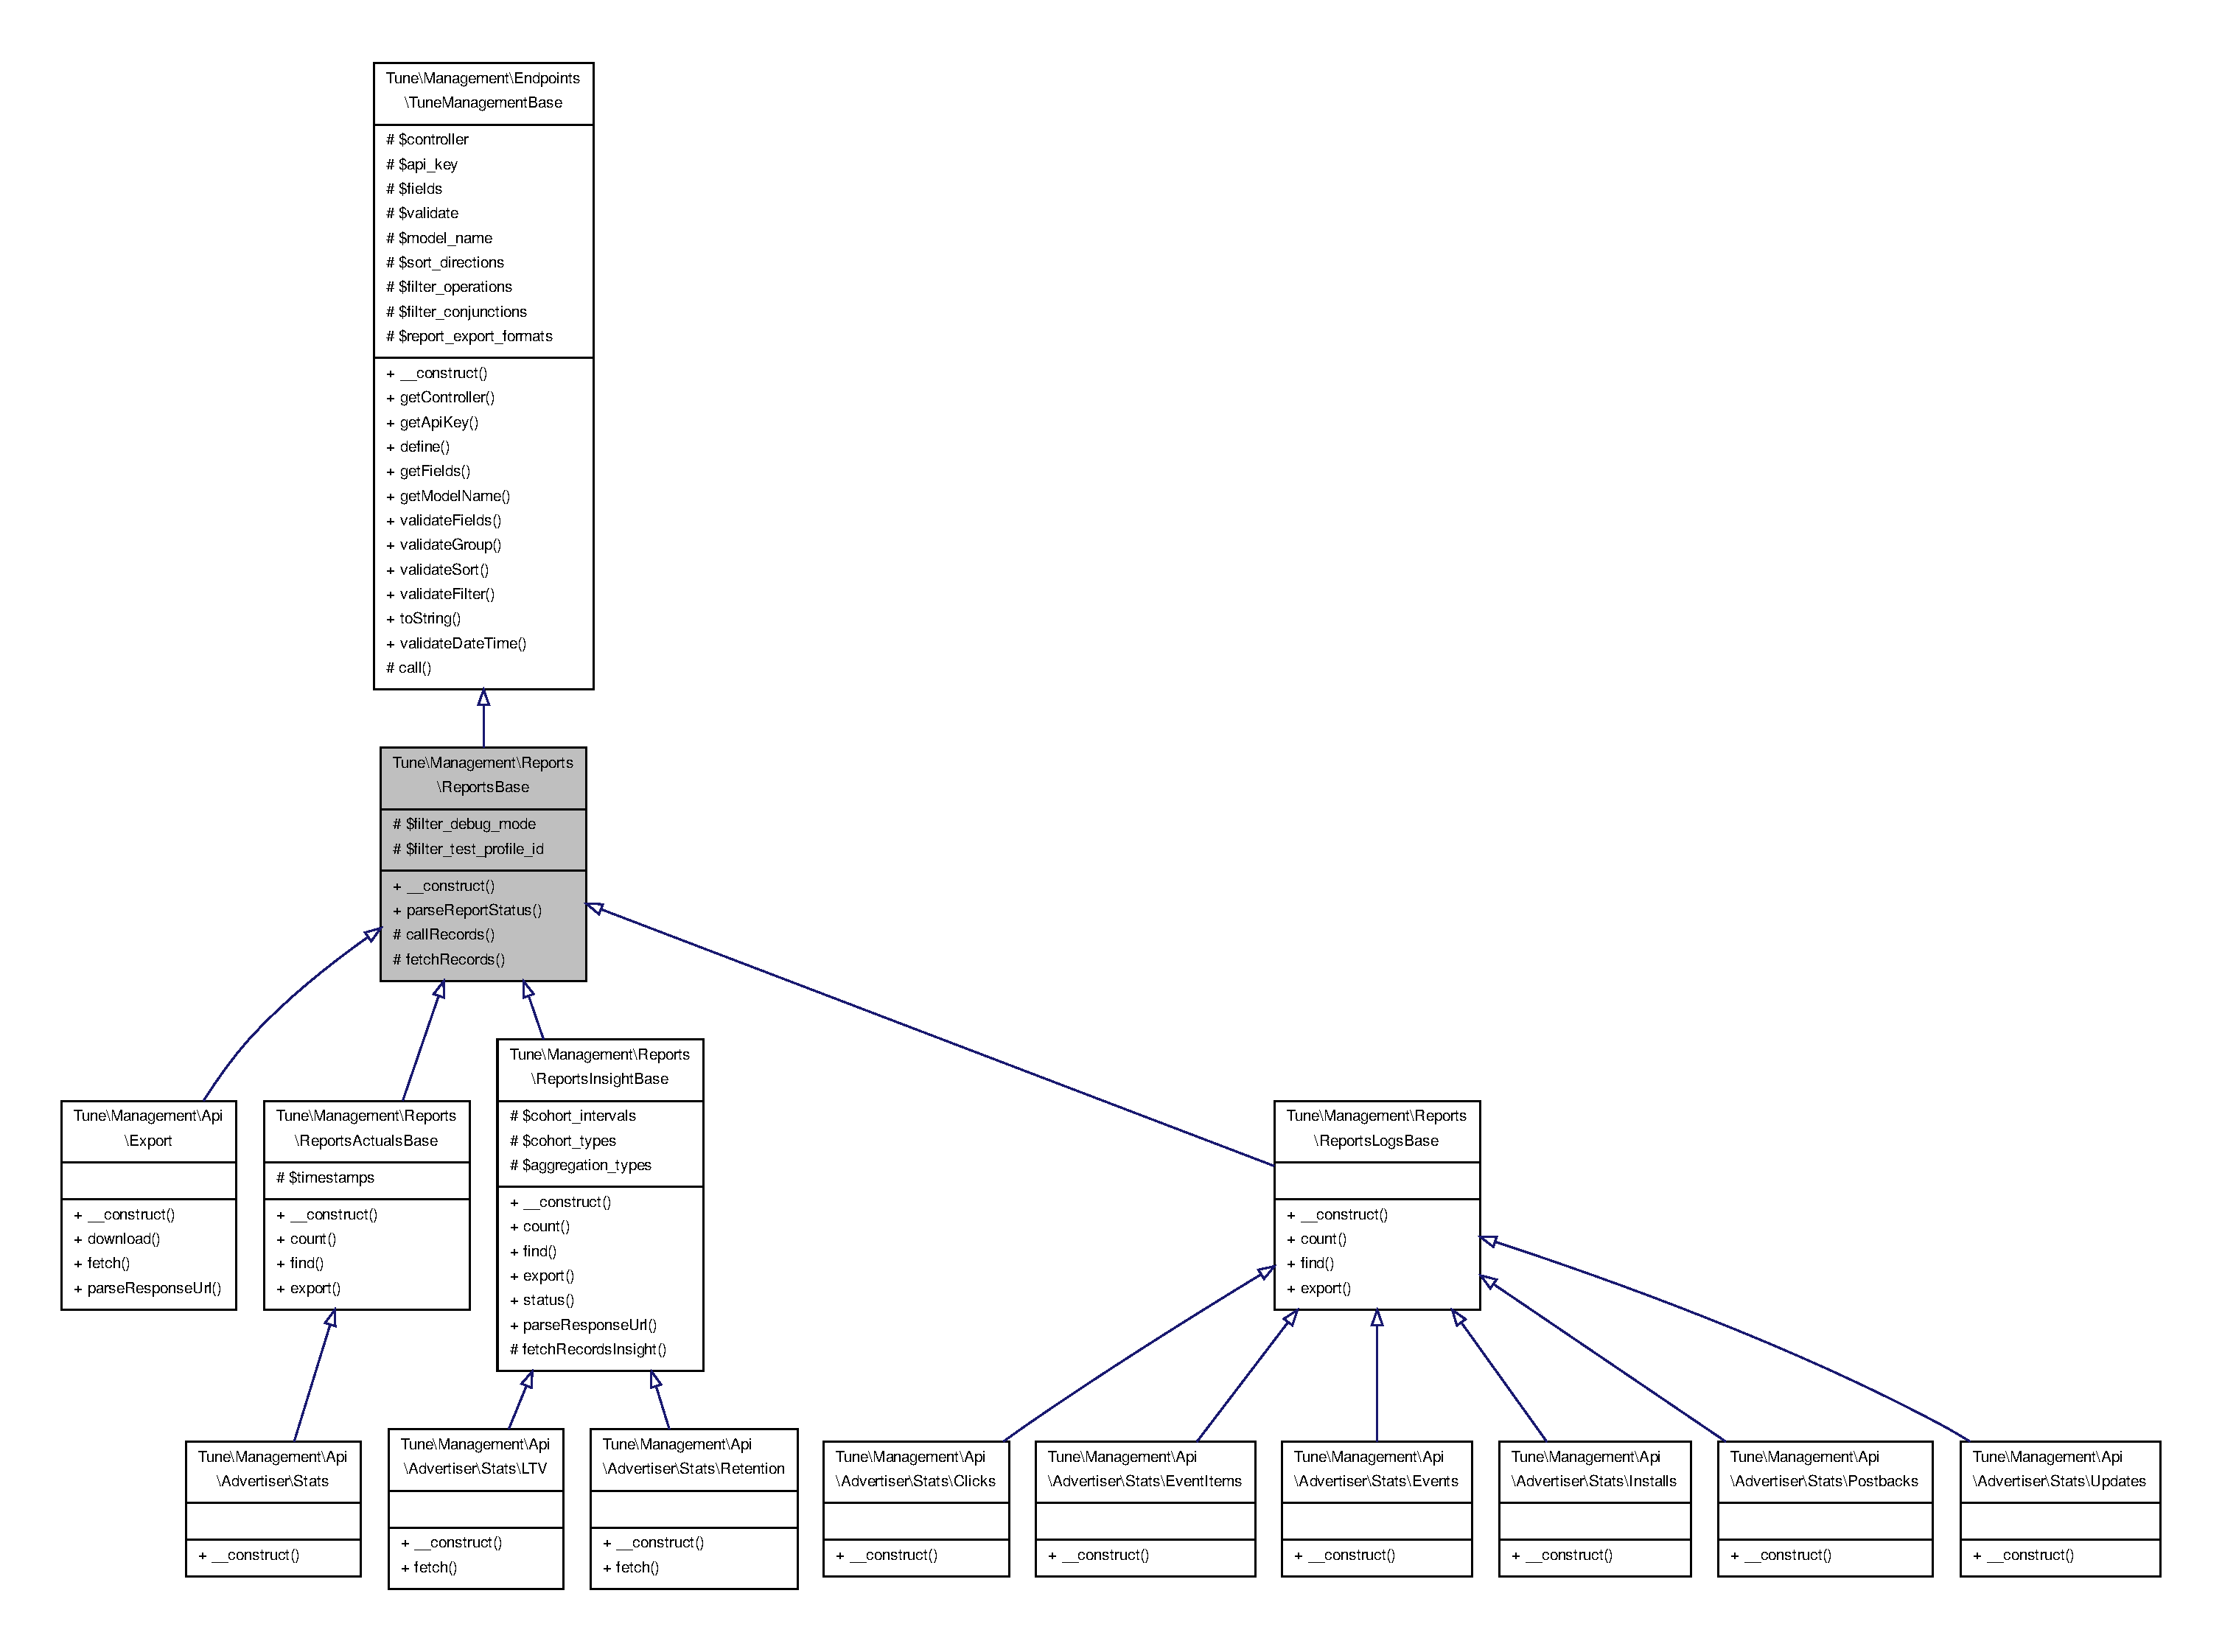
\includegraphics[width=350pt]{classTune_1_1Management_1_1Reports_1_1ReportsBase__inherit__graph}
\end{center}
\end{figure}


Collaboration diagram for Tune\textbackslash{}Management\textbackslash{}Reports\textbackslash{}Reports\-Base\-:
\nopagebreak
\begin{figure}[H]
\begin{center}
\leavevmode
\includegraphics[height=550pt]{classTune_1_1Management_1_1Reports_1_1ReportsBase__coll__graph}
\end{center}
\end{figure}
\subsection*{Public Member Functions}
\begin{DoxyCompactItemize}
\item 
\hyperlink{classTune_1_1Management_1_1Reports_1_1ReportsBase_a09c4290191dba390e46ba730ce564cee}{\-\_\-\-\_\-construct} (\$controller, \$api\-\_\-key, \$filter\-\_\-debug\-\_\-mode, \$filter\-\_\-test\-\_\-profile\-\_\-id, \$validate=false)
\begin{DoxyCompactList}\small\item\em Constructor. \end{DoxyCompactList}\item 
\hyperlink{classTune_1_1Management_1_1Reports_1_1ReportsBase_a5cebfc222eef4019fcf3a428de5adcfe}{parse\-Report\-Status} (\$report\-\_\-url, \$report\-\_\-format)
\begin{DoxyCompactList}\small\item\em Helper function for fetching report document given provided job identifier. \end{DoxyCompactList}\end{DoxyCompactItemize}
\subsection*{Protected Member Functions}
\begin{DoxyCompactItemize}
\item 
\hyperlink{classTune_1_1Management_1_1Reports_1_1ReportsBase_aecd8c7a22f4740abab9bd0feabc15387}{call\-Records} (\$action, \$query\-\_\-string\-\_\-dict)
\begin{DoxyCompactList}\small\item\em Prepare action with provided query string parameters, then call \hyperlink{namespaceTune_1_1Management}{Management} A\-P\-I service. \end{DoxyCompactList}\item 
\hyperlink{classTune_1_1Management_1_1Reports_1_1ReportsBase_ac6c3a238e99b0dfb88a83fc70924493b}{fetch\-Records} (\$mod\-\_\-export\-\_\-class, \$mod\-\_\-export\-\_\-function, \$job\-\_\-id, \$report\-\_\-format, \$verbose=false, \$sleep=60)
\begin{DoxyCompactList}\small\item\em Helper function for fetching report document given provided job identifier. \end{DoxyCompactList}\end{DoxyCompactItemize}
\subsection*{Protected Attributes}
\begin{DoxyCompactItemize}
\item 
\hyperlink{classTune_1_1Management_1_1Reports_1_1ReportsBase_a6dde408a407042ce3f665e9f16f386b1}{\$filter\-\_\-debug\-\_\-mode} = false
\item 
\hyperlink{classTune_1_1Management_1_1Reports_1_1ReportsBase_a2a621a3704fdccb98094c2f94bc6180e}{\$filter\-\_\-test\-\_\-profile\-\_\-id} = false
\end{DoxyCompactItemize}
\subsection*{Additional Inherited Members}


\subsection{Detailed Description}


Definition at line 49 of file Reports\-Base.\-php.



\subsection{Constructor \& Destructor Documentation}
\hypertarget{classTune_1_1Management_1_1Reports_1_1ReportsBase_a09c4290191dba390e46ba730ce564cee}{\index{Tune\-::\-Management\-::\-Reports\-::\-Reports\-Base@{Tune\-::\-Management\-::\-Reports\-::\-Reports\-Base}!\-\_\-\-\_\-construct@{\-\_\-\-\_\-construct}}
\index{\-\_\-\-\_\-construct@{\-\_\-\-\_\-construct}!Tune::Management::Reports::ReportsBase@{Tune\-::\-Management\-::\-Reports\-::\-Reports\-Base}}
\subsubsection[{\-\_\-\-\_\-construct}]{\setlength{\rightskip}{0pt plus 5cm}Tune\textbackslash{}\-Management\textbackslash{}\-Reports\textbackslash{}\-Reports\-Base\-::\-\_\-\-\_\-construct (
\begin{DoxyParamCaption}
\item[{}]{\$controller, }
\item[{}]{\$api\-\_\-key, }
\item[{}]{\$filter\-\_\-debug\-\_\-mode, }
\item[{}]{\$filter\-\_\-test\-\_\-profile\-\_\-id, }
\item[{}]{\$validate = {\ttfamily false}}
\end{DoxyParamCaption}
)}}\label{classTune_1_1Management_1_1Reports_1_1ReportsBase_a09c4290191dba390e46ba730ce564cee}


Constructor. 


\begin{DoxyParams}[1]{Parameters}
string & {\em \$controller} & \hyperlink{namespaceTune}{Tune} \hyperlink{namespaceTune_1_1Management}{Management} A\-P\-I endpoint name. \\
\hline
string & {\em \$api\-\_\-key} & Mobile\-App\-Tracking A\-P\-I Key. \\
\hline
bool & {\em \$filter\-\_\-debug\-\_\-mode} & Remove debug mode information from results. \\
\hline
bool & {\em \$filter\-\_\-test\-\_\-profile\-\_\-id} & Remove test profile information from results. \\
\hline
bool & {\em \$validate} & Validate fields used by actions' parameters. \\
\hline
\end{DoxyParams}


Definition at line 71 of file Reports\-Base.\-php.


\begin{DoxyCode}
77       \{
78         \textcolor{comment}{// controller}
79         \textcolor{keywordflow}{if} (!is\_string(\hyperlink{classTune_1_1Management_1_1Endpoints_1_1TuneManagementBase_a8a73dbafcc91b04d7f1a7e2aaa9b486a}{$controller}) || empty(\hyperlink{classTune_1_1Management_1_1Endpoints_1_1TuneManagementBase_a8a73dbafcc91b04d7f1a7e2aaa9b486a}{$controller})) \{
80             \textcolor{keywordflow}{throw} new \(\backslash\)InvalidArgumentException(\textcolor{stringliteral}{"Parameter 'controller' is not defined."});
81         \}
82         \textcolor{comment}{// api\_key}
83         \textcolor{keywordflow}{if} (!is\_string(\hyperlink{classTune_1_1Management_1_1Endpoints_1_1TuneManagementBase_ac53649b4bc72055e1d55e53e0b6f244e}{$api\_key}) || empty(\hyperlink{classTune_1_1Management_1_1Endpoints_1_1TuneManagementBase_ac53649b4bc72055e1d55e53e0b6f244e}{$api\_key})) \{
84             \textcolor{keywordflow}{throw} new \(\backslash\)InvalidArgumentException(\textcolor{stringliteral}{"Parameter 'api\_key' is not defined."});
85         \}
86         \textcolor{comment}{// filter\_debug\_mode}
87         \textcolor{keywordflow}{if} (!is\_bool(\hyperlink{classTune_1_1Management_1_1Endpoints_1_1TuneManagementBase_a264eed27b0a1c963808fc7eab6da98bc}{$validate})) \{
88             \textcolor{keywordflow}{throw} new \(\backslash\)InvalidArgumentException(\textcolor{stringliteral}{"Parameter 'validate' is not defined as a bool."});
89         \}
90         \textcolor{comment}{// filter\_debug\_mode}
91         \textcolor{keywordflow}{if} (!is\_bool(\hyperlink{classTune_1_1Management_1_1Reports_1_1ReportsBase_a6dde408a407042ce3f665e9f16f386b1}{$filter\_debug\_mode})) \{
92             \textcolor{keywordflow}{throw} new \(\backslash\)InvalidArgumentException(\textcolor{stringliteral}{"Parameter 'filter\_debug\_mode' is not defined as a bool."});
93         \}
94         \textcolor{comment}{// filter\_test\_profile\_id}
95         \textcolor{keywordflow}{if} (!is\_bool(\hyperlink{classTune_1_1Management_1_1Reports_1_1ReportsBase_a2a621a3704fdccb98094c2f94bc6180e}{$filter\_test\_profile\_id})) \{
96             \textcolor{keywordflow}{throw} new \(\backslash\)InvalidArgumentException(\textcolor{stringliteral}{"Parameter 'filter\_test\_profile\_id' is not defined as a
       bool."});
97         \}
98 
99         $this->filter\_debug\_mode = \hyperlink{classTune_1_1Management_1_1Reports_1_1ReportsBase_a6dde408a407042ce3f665e9f16f386b1}{$filter\_debug\_mode};
100         $this->filter\_test\_profile\_id = \hyperlink{classTune_1_1Management_1_1Reports_1_1ReportsBase_a2a621a3704fdccb98094c2f94bc6180e}{$filter\_test\_profile\_id};
101 
102         parent::\_\_construct(\hyperlink{classTune_1_1Management_1_1Endpoints_1_1TuneManagementBase_a8a73dbafcc91b04d7f1a7e2aaa9b486a}{$controller}, \hyperlink{classTune_1_1Management_1_1Endpoints_1_1TuneManagementBase_ac53649b4bc72055e1d55e53e0b6f244e}{$api\_key}, \hyperlink{classTune_1_1Management_1_1Endpoints_1_1TuneManagementBase_a264eed27b0a1c963808fc7eab6da98bc}{$validate});
103     \}
\end{DoxyCode}


\subsection{Member Function Documentation}
\hypertarget{classTune_1_1Management_1_1Reports_1_1ReportsBase_aecd8c7a22f4740abab9bd0feabc15387}{\index{Tune\-::\-Management\-::\-Reports\-::\-Reports\-Base@{Tune\-::\-Management\-::\-Reports\-::\-Reports\-Base}!call\-Records@{call\-Records}}
\index{call\-Records@{call\-Records}!Tune::Management::Reports::ReportsBase@{Tune\-::\-Management\-::\-Reports\-::\-Reports\-Base}}
\subsubsection[{call\-Records}]{\setlength{\rightskip}{0pt plus 5cm}Tune\textbackslash{}\-Management\textbackslash{}\-Reports\textbackslash{}\-Reports\-Base\-::call\-Records (
\begin{DoxyParamCaption}
\item[{}]{\$action, }
\item[{}]{\$query\-\_\-string\-\_\-dict}
\end{DoxyParamCaption}
)\hspace{0.3cm}{\ttfamily [protected]}}}\label{classTune_1_1Management_1_1Reports_1_1ReportsBase_aecd8c7a22f4740abab9bd0feabc15387}


Prepare action with provided query string parameters, then call \hyperlink{namespaceTune_1_1Management}{Management} A\-P\-I service. 


\begin{DoxyParams}[1]{Parameters}
string & {\em \$action} & Endpoint action to be called. \\
\hline
dict & {\em \$query\-\_\-string\-\_\-dict} & Query string parameters for this action.\\
\hline
\end{DoxyParams}

\begin{DoxyExceptions}{Exceptions}
{\em \textbackslash{}\-Invalid\-Argument\-Exception} & \\
\hline
\end{DoxyExceptions}


Definition at line 114 of file Reports\-Base.\-php.


\begin{DoxyCode}
117       \{
118         \textcolor{comment}{// action}
119         \textcolor{keywordflow}{if} (!is\_string($action) || empty($action)) \{
120             \textcolor{keywordflow}{throw} new \(\backslash\)InvalidArgumentException(\textcolor{stringliteral}{"Parameter 'action' is not defined."});
121         \}
122         \textcolor{keywordflow}{if} (is\_null($query\_string\_dict) && !is\_array($query\_string\_dict)) \{
123             \textcolor{keywordflow}{throw} new \(\backslash\)InvalidArgumentException(\textcolor{stringliteral}{"Parameter 'query\_string\_dict' is not defined as
       associative array."});
124         \}
125 
126         $sdk\_filter = null;
127 
128         \textcolor{keywordflow}{if} ($this->filter\_debug\_mode or $this->filter\_test\_profile\_id) \{
129             $sdk\_filter = null;
130             \textcolor{keywordflow}{if} ($this->filter\_debug\_mode) \{
131                 $sdk\_filter = \textcolor{stringliteral}{"(debug\_mode=0 OR debug\_mode is NULL)"};
132             \}
133 
134             \textcolor{keywordflow}{if} ($this->filter\_test\_profile\_id) \{
135                 \textcolor{keywordflow}{if} (!is\_null($sdk\_filter) && is\_string($sdk\_filter) && !empty($sdk\_filter)) \{
136                     $sdk\_filter .= \textcolor{stringliteral}{" AND "};
137                 \}
138 
139                 $sdk\_filter = \textcolor{stringliteral}{"(test\_profile\_id=0 OR test\_profile\_id IS NULL)"};
140             \}
141         \}
142 
143         \textcolor{keywordflow}{if} (!is\_null($sdk\_filter) && is\_string($sdk\_filter) && !empty($sdk\_filter)) \{
144             \textcolor{keywordflow}{if} (array\_key\_exists(\textcolor{stringliteral}{'filter'}, $query\_string\_dict)) \{
145                 \textcolor{keywordflow}{if} (!is\_null($query\_string\_dict[\textcolor{stringliteral}{'filter'}])
146                     && is\_string($query\_string\_dict[\textcolor{stringliteral}{'filter'}])
147                     && !empty($query\_string\_dict[\textcolor{stringliteral}{'filter'}])) \{
148                     $query\_string\_dict[\textcolor{stringliteral}{'filter'}] = \textcolor{stringliteral}{"("} . $query\_string\_dict[\textcolor{stringliteral}{'filter'}] . \textcolor{stringliteral}{") AND "} . 
      $sdk\_filter;
149                 \} \textcolor{keywordflow}{else} \{
150                     $query\_string\_dict[\textcolor{stringliteral}{'filter'}] = $sdk\_filter;
151                 \}
152             \} \textcolor{keywordflow}{else} \{
153                 $query\_string\_dict[\textcolor{stringliteral}{'filter'}] = $sdk\_filter;
154             \}
155         \}
156 
157         \textcolor{keywordflow}{if} (array\_key\_exists(\textcolor{stringliteral}{'filter'}, $query\_string\_dict)) \{
158             \textcolor{keywordflow}{if} (!is\_null($query\_string\_dict[\textcolor{stringliteral}{'filter'}])
159                 && is\_string($query\_string\_dict[\textcolor{stringliteral}{'filter'}])
160                 && !empty($query\_string\_dict[\textcolor{stringliteral}{'filter'}])) \{
161                 $query\_string\_dict[\textcolor{stringliteral}{'filter'}] = \textcolor{stringliteral}{"("} . $query\_string\_dict[\textcolor{stringliteral}{'filter'}] . \textcolor{stringliteral}{")"};
162             \}
163         \}
164 
165         \textcolor{keywordflow}{return} parent::call($action, $query\_string\_dict);
166     \}
\end{DoxyCode}
\hypertarget{classTune_1_1Management_1_1Reports_1_1ReportsBase_ac6c3a238e99b0dfb88a83fc70924493b}{\index{Tune\-::\-Management\-::\-Reports\-::\-Reports\-Base@{Tune\-::\-Management\-::\-Reports\-::\-Reports\-Base}!fetch\-Records@{fetch\-Records}}
\index{fetch\-Records@{fetch\-Records}!Tune::Management::Reports::ReportsBase@{Tune\-::\-Management\-::\-Reports\-::\-Reports\-Base}}
\subsubsection[{fetch\-Records}]{\setlength{\rightskip}{0pt plus 5cm}Tune\textbackslash{}\-Management\textbackslash{}\-Reports\textbackslash{}\-Reports\-Base\-::fetch\-Records (
\begin{DoxyParamCaption}
\item[{}]{\$mod\-\_\-export\-\_\-class, }
\item[{}]{\$mod\-\_\-export\-\_\-function, }
\item[{}]{\$job\-\_\-id, }
\item[{}]{\$report\-\_\-format, }
\item[{}]{\$verbose = {\ttfamily false}, }
\item[{}]{\$sleep = {\ttfamily 60}}
\end{DoxyParamCaption}
)\hspace{0.3cm}{\ttfamily [protected]}}}\label{classTune_1_1Management_1_1Reports_1_1ReportsBase_ac6c3a238e99b0dfb88a83fc70924493b}


Helper function for fetching report document given provided job identifier. 

Requesting for report url is not the same for all report endpoints.


\begin{DoxyParams}[1]{Parameters}
string & {\em \$mod\-\_\-export\-\_\-class} & Report class. \\
\hline
string & {\em \$mod\-\_\-export\-\_\-function} & Report function performing status request. \\
\hline
string & {\em \$job\-\_\-id} & Job Identifier of report on queue. \\
\hline
string & {\em \$report\-\_\-format} & Requested document format\-: csv, json \\
\hline
bool & {\em \$verbose} & For debugging purposes only. \\
\hline
int & {\em \$sleep} & How long thread should sleep before next status request.\\
\hline
\end{DoxyParams}
\begin{DoxyReturn}{Returns}
object Report reader 
\end{DoxyReturn}

\begin{DoxyExceptions}{Exceptions}
{\em \textbackslash{}\-Invalid\-Argument\-Exception} & \\
\hline
{\em Tune\-Service\-Exception} & \\
\hline
\end{DoxyExceptions}


Definition at line 185 of file Reports\-Base.\-php.


\begin{DoxyCode}
192       \{
193         \textcolor{keywordflow}{if} (!is\_string($mod\_export\_class) || empty($mod\_export\_class)) \{
194             \textcolor{keywordflow}{throw} new \(\backslash\)InvalidArgumentException(\textcolor{stringliteral}{"Parameter 'mod\_export\_class' is not defined."});
195         \}
196         \textcolor{keywordflow}{if} (!is\_string($mod\_export\_function) || empty($mod\_export\_function)) \{
197             \textcolor{keywordflow}{throw} new \(\backslash\)InvalidArgumentException(\textcolor{stringliteral}{"Parameter 'mod\_export\_function' is not defined."});
198         \}
199         \textcolor{keywordflow}{if} (!is\_string($job\_id) || empty($job\_id)) \{
200             \textcolor{keywordflow}{throw} new \(\backslash\)InvalidArgumentException(\textcolor{stringliteral}{"Parameter 'job\_id' is not defined."});
201         \}
202         \textcolor{keywordflow}{if} (!is\_string($report\_format) || empty($report\_format)) \{
203             \textcolor{keywordflow}{throw} new \(\backslash\)InvalidArgumentException(\textcolor{stringliteral}{"Parameter 'job\_id' is not defined."});
204         \}
205         \textcolor{keywordflow}{if} (!is\_string(parent::getApiKey()) || empty(parent::getApiKey())) \{
206             \textcolor{keywordflow}{throw} new \(\backslash\)InvalidArgumentException(\textcolor{stringliteral}{"Parameter 'api\_key' is not defined."});
207         \}
208 
209         $export\_worker = \textcolor{keyword}{new} ReportExportWorker(
210             $mod\_export\_class,
211             $mod\_export\_function,
212             $this->api\_key,
213             $job\_id,
214             $verbose,
215             $sleep
216         );
217 
218         \textcolor{keywordflow}{if} ($verbose) \{
219             echo \textcolor{stringliteral}{"Starting thread..."} . PHP\_EOL;
220         \}
221         $export\_worker->start();
222         \textcolor{keywordflow}{if} ($verbose) \{
223             echo \textcolor{stringliteral}{"Waiting..."} . PHP\_EOL;
224         \}
225         \textcolor{comment}{// Calling context to wait for the referenced Thread to finish executing}
226         $success = $export\_worker->join();
227 
228         \textcolor{keywordflow}{if} ($verbose && $success) \{
229             echo \textcolor{stringliteral}{"Thread completed successfully."} . PHP\_EOL;
230         \}
231 
232         $response = $export\_worker->getResponse();
233 
234         \textcolor{keywordflow}{if} (!$success) \{
235             \textcolor{keywordflow}{throw} \textcolor{keyword}{new} TuneSdkException(\textcolor{stringliteral}{"Thread failed to complete successfully: "} + print\_r($response, \textcolor{keyword}{true}
      ) . PHP\_EOL);
236         \}
237 
238         \textcolor{keywordflow}{if} (is\_null($response)
239             || $response->getHttpCode() != 200
240             || $response->getData()[\textcolor{stringliteral}{"status"}] == \textcolor{stringliteral}{"fail"}
241         ) \{
242             \textcolor{keywordflow}{throw} \textcolor{keyword}{new} TuneServiceException(\textcolor{stringliteral}{"Report request failed: "} + print\_r($response, \textcolor{keyword}{true}) . PHP\_EOL);
243         \}
244 
245         $report\_url = $mod\_export\_class::parseResponseUrl($response);
246 
247         \textcolor{keywordflow}{if} (!is\_string($report\_url) || empty($report\_url)) \{
248             \textcolor{keywordflow}{throw} \textcolor{keyword}{new} TuneSdkException(\textcolor{stringliteral}{"Failed to get report Url from response."});
249         \}
250 
251         \textcolor{keywordflow}{if} ($verbose) \{
252             echo \textcolor{stringliteral}{"Completed report request: "} + print\_r($response, \textcolor{keyword}{true}) . PHP\_EOL;
253         \}
254 
255         \textcolor{keywordflow}{return} $this->\hyperlink{classTune_1_1Management_1_1Reports_1_1ReportsBase_a5cebfc222eef4019fcf3a428de5adcfe}{parseReportStatus}($report\_url, $report\_format);
256     \}
\end{DoxyCode}


Here is the call graph for this function\-:
\nopagebreak
\begin{figure}[H]
\begin{center}
\leavevmode
\includegraphics[width=350pt]{classTune_1_1Management_1_1Reports_1_1ReportsBase_ac6c3a238e99b0dfb88a83fc70924493b_cgraph}
\end{center}
\end{figure}


\hypertarget{classTune_1_1Management_1_1Reports_1_1ReportsBase_a5cebfc222eef4019fcf3a428de5adcfe}{\index{Tune\-::\-Management\-::\-Reports\-::\-Reports\-Base@{Tune\-::\-Management\-::\-Reports\-::\-Reports\-Base}!parse\-Report\-Status@{parse\-Report\-Status}}
\index{parse\-Report\-Status@{parse\-Report\-Status}!Tune::Management::Reports::ReportsBase@{Tune\-::\-Management\-::\-Reports\-::\-Reports\-Base}}
\subsubsection[{parse\-Report\-Status}]{\setlength{\rightskip}{0pt plus 5cm}Tune\textbackslash{}\-Management\textbackslash{}\-Reports\textbackslash{}\-Reports\-Base\-::parse\-Report\-Status (
\begin{DoxyParamCaption}
\item[{}]{\$report\-\_\-url, }
\item[{}]{\$report\-\_\-format}
\end{DoxyParamCaption}
)}}\label{classTune_1_1Management_1_1Reports_1_1ReportsBase_a5cebfc222eef4019fcf3a428de5adcfe}


Helper function for fetching report document given provided job identifier. 

Response is not the same for all report endpoints.


\begin{DoxyParams}[1]{Parameters}
string & {\em \$report\-\_\-url} & Report url provided upon completing of export processing. \\
\hline
string & {\em \$report\-\_\-format} & Expected format of exported report.\\
\hline
\end{DoxyParams}
\begin{DoxyReturn}{Returns}
null 
\end{DoxyReturn}

\begin{DoxyExceptions}{Exceptions}
{\em Tune\-Sdk\-Exception} & \\
\hline
\end{DoxyExceptions}


Definition at line 269 of file Reports\-Base.\-php.


\begin{DoxyCode}
272       \{
273         $report\_reader = null;
274         \textcolor{keywordflow}{try} \{
275             \textcolor{keywordflow}{if} ($report\_format == \textcolor{stringliteral}{"csv"}) \{
276                 $report\_reader = \textcolor{keyword}{new} ReportReaderCSV(
277                     $report\_url
278                 );
279             \} elseif ($report\_format == \textcolor{stringliteral}{"json"}) \{
280                 $report\_reader = \textcolor{keyword}{new} ReportReaderJSON(
281                     $report\_url
282                 );
283             \}
284         \} \textcolor{keywordflow}{catch} (\hyperlink{classException}{Exception} $ex) \{
285             \textcolor{keywordflow}{throw} \textcolor{keyword}{new} TuneSdkException(
286                 \textcolor{stringliteral}{"Failed to create reader provided by url \{$report\_url\}: "} + print\_r($ex, \textcolor{keyword}{true}) . PHP\_EOL
287             );
288         \}
289 
290         \textcolor{keywordflow}{return} $report\_reader;
291     \}
\end{DoxyCode}


Here is the caller graph for this function\-:
\nopagebreak
\begin{figure}[H]
\begin{center}
\leavevmode
\includegraphics[width=350pt]{classTune_1_1Management_1_1Reports_1_1ReportsBase_a5cebfc222eef4019fcf3a428de5adcfe_icgraph}
\end{center}
\end{figure}




\subsection{Field Documentation}
\hypertarget{classTune_1_1Management_1_1Reports_1_1ReportsBase_a6dde408a407042ce3f665e9f16f386b1}{\index{Tune\-::\-Management\-::\-Reports\-::\-Reports\-Base@{Tune\-::\-Management\-::\-Reports\-::\-Reports\-Base}!\$filter\-\_\-debug\-\_\-mode@{\$filter\-\_\-debug\-\_\-mode}}
\index{\$filter\-\_\-debug\-\_\-mode@{\$filter\-\_\-debug\-\_\-mode}!Tune::Management::Reports::ReportsBase@{Tune\-::\-Management\-::\-Reports\-::\-Reports\-Base}}
\subsubsection[{\$filter\-\_\-debug\-\_\-mode}]{\setlength{\rightskip}{0pt plus 5cm}Tune\textbackslash{}\-Management\textbackslash{}\-Reports\textbackslash{}\-Reports\-Base\-::\$filter\-\_\-debug\-\_\-mode = false\hspace{0.3cm}{\ttfamily [protected]}}}\label{classTune_1_1Management_1_1Reports_1_1ReportsBase_a6dde408a407042ce3f665e9f16f386b1}


Definition at line 55 of file Reports\-Base.\-php.

\hypertarget{classTune_1_1Management_1_1Reports_1_1ReportsBase_a2a621a3704fdccb98094c2f94bc6180e}{\index{Tune\-::\-Management\-::\-Reports\-::\-Reports\-Base@{Tune\-::\-Management\-::\-Reports\-::\-Reports\-Base}!\$filter\-\_\-test\-\_\-profile\-\_\-id@{\$filter\-\_\-test\-\_\-profile\-\_\-id}}
\index{\$filter\-\_\-test\-\_\-profile\-\_\-id@{\$filter\-\_\-test\-\_\-profile\-\_\-id}!Tune::Management::Reports::ReportsBase@{Tune\-::\-Management\-::\-Reports\-::\-Reports\-Base}}
\subsubsection[{\$filter\-\_\-test\-\_\-profile\-\_\-id}]{\setlength{\rightskip}{0pt plus 5cm}Tune\textbackslash{}\-Management\textbackslash{}\-Reports\textbackslash{}\-Reports\-Base\-::\$filter\-\_\-test\-\_\-profile\-\_\-id = false\hspace{0.3cm}{\ttfamily [protected]}}}\label{classTune_1_1Management_1_1Reports_1_1ReportsBase_a2a621a3704fdccb98094c2f94bc6180e}


Definition at line 60 of file Reports\-Base.\-php.



The documentation for this class was generated from the following file\-:\begin{DoxyCompactItemize}
\item 
lib/\-Tune/\-Management/\-Reports/\hyperlink{ReportsBase_8php}{Reports\-Base.\-php}\end{DoxyCompactItemize}

\hypertarget{classTune_1_1Management_1_1Reports_1_1ReportsInsightBase}{\section{Tune\textbackslash{}Management\textbackslash{}Reports\textbackslash{}Reports\-Insight\-Base Class Reference}
\label{classTune_1_1Management_1_1Reports_1_1ReportsInsightBase}\index{Tune\textbackslash{}\-Management\textbackslash{}\-Reports\textbackslash{}\-Reports\-Insight\-Base@{Tune\textbackslash{}\-Management\textbackslash{}\-Reports\textbackslash{}\-Reports\-Insight\-Base}}
}


Inheritance diagram for Tune\textbackslash{}Management\textbackslash{}Reports\textbackslash{}Reports\-Insight\-Base\-:
\nopagebreak
\begin{figure}[H]
\begin{center}
\leavevmode
\includegraphics[height=550pt]{classTune_1_1Management_1_1Reports_1_1ReportsInsightBase__inherit__graph}
\end{center}
\end{figure}


Collaboration diagram for Tune\textbackslash{}Management\textbackslash{}Reports\textbackslash{}Reports\-Insight\-Base\-:
\nopagebreak
\begin{figure}[H]
\begin{center}
\leavevmode
\includegraphics[height=550pt]{classTune_1_1Management_1_1Reports_1_1ReportsInsightBase__coll__graph}
\end{center}
\end{figure}
\subsection*{Public Member Functions}
\begin{DoxyCompactItemize}
\item 
\hyperlink{classTune_1_1Management_1_1Reports_1_1ReportsInsightBase_a4f2d06123aa69e69e8240e819364f425}{\-\_\-\-\_\-construct} (\$controller, \$api\-\_\-key, \$filter\-\_\-debug\-\_\-mode, \$filter\-\_\-test\-\_\-profile\-\_\-id, \$validate=false)
\begin{DoxyCompactList}\small\item\em Constructor. \end{DoxyCompactList}\item 
\hyperlink{classTune_1_1Management_1_1Reports_1_1ReportsInsightBase_aa8ef42d5b10d3540865969437261d090}{count} (\$start\-\_\-date, \$end\-\_\-date, \$cohort\-\_\-type, \$group, \$cohort\-\_\-interval=null, \$filter=null, \$response\-\_\-timezone=null)
\begin{DoxyCompactList}\small\item\em Counts all existing records that match filter criteria and returns an array of found model data. \end{DoxyCompactList}\item 
\hyperlink{classTune_1_1Management_1_1Reports_1_1ReportsInsightBase_a1cb8a128711b32efb903194dd84e8af6}{find} (\$start\-\_\-date, \$end\-\_\-date, \$cohort\-\_\-type, \$aggregation\-\_\-type, \$group, \$cohort\-\_\-interval=null, \$filter=null, \$fields=null, \$limit=null, \$page=null, \$sort=null, \$format=null, \$response\-\_\-timezone=null)
\begin{DoxyCompactList}\small\item\em Finds all existing records that match filter criteria and returns an array of found model data. \end{DoxyCompactList}\item 
\hyperlink{classTune_1_1Management_1_1Reports_1_1ReportsInsightBase_a3e56e5dd9984ec0ff20db6a21de4f455}{export} (\$start\-\_\-date, \$end\-\_\-date, \$cohort\-\_\-type, \$aggregation\-\_\-type, \$group, \$fields, \$cohort\-\_\-interval=null, \$filter=null, \$response\-\_\-timezone=null)
\begin{DoxyCompactList}\small\item\em Places a job into a queue to generate a report that will contain records that match provided filter criteria, and it returns a job identifier to be provided to action /export/download.json to download completed report. \end{DoxyCompactList}\item 
\hyperlink{classTune_1_1Management_1_1Reports_1_1ReportsInsightBase_aaae96a8b5716cb100ed34e37004a70ca}{status} (\$job\-\_\-id)
\begin{DoxyCompactList}\small\item\em Query status of insight reports. \end{DoxyCompactList}\end{DoxyCompactItemize}
\subsection*{Static Public Member Functions}
\begin{DoxyCompactItemize}
\item 
static \hyperlink{classTune_1_1Management_1_1Reports_1_1ReportsInsightBase_a8af44833abc5829a74168bec5cdb5dc7}{parse\-Response\-Url} (\$response)
\begin{DoxyCompactList}\small\item\em Helper function for parsing export status response to gather report url. \end{DoxyCompactList}\end{DoxyCompactItemize}
\subsection*{Protected Member Functions}
\begin{DoxyCompactItemize}
\item 
\hyperlink{classTune_1_1Management_1_1Reports_1_1ReportsInsightBase_a0de324106185ce1477111745f84c4a85}{fetch\-Records\-Insight} (\$mod\-\_\-export\-\_\-class, \$job\-\_\-id, \$report\-\_\-format=\char`\"{}csv\char`\"{}, \$verbose=false, \$sleep=10)
\begin{DoxyCompactList}\small\item\em Helper function for fetching report upon completion. \end{DoxyCompactList}\end{DoxyCompactItemize}
\subsection*{Static Protected Attributes}
\begin{DoxyCompactItemize}
\item 
static \hyperlink{classTune_1_1Management_1_1Reports_1_1ReportsInsightBase_a4b54d97ffa0b522f9ab30425fc595ba7}{\$cohort\-\_\-intervals}
\item 
static \hyperlink{classTune_1_1Management_1_1Reports_1_1ReportsInsightBase_a1d7559051fef0f083d7d33ae18aaa6d6}{\$cohort\-\_\-types}
\item 
static \hyperlink{classTune_1_1Management_1_1Reports_1_1ReportsInsightBase_a4c40a9cd27f07ec535e6c51bad40e845}{\$aggregation\-\_\-types}
\end{DoxyCompactItemize}
\subsection*{Additional Inherited Members}


\subsection{Detailed Description}


Definition at line 44 of file Reports\-Insight\-Base.\-php.



\subsection{Constructor \& Destructor Documentation}
\hypertarget{classTune_1_1Management_1_1Reports_1_1ReportsInsightBase_a4f2d06123aa69e69e8240e819364f425}{\index{Tune\-::\-Management\-::\-Reports\-::\-Reports\-Insight\-Base@{Tune\-::\-Management\-::\-Reports\-::\-Reports\-Insight\-Base}!\-\_\-\-\_\-construct@{\-\_\-\-\_\-construct}}
\index{\-\_\-\-\_\-construct@{\-\_\-\-\_\-construct}!Tune::Management::Reports::ReportsInsightBase@{Tune\-::\-Management\-::\-Reports\-::\-Reports\-Insight\-Base}}
\subsubsection[{\-\_\-\-\_\-construct}]{\setlength{\rightskip}{0pt plus 5cm}Tune\textbackslash{}\-Management\textbackslash{}\-Reports\textbackslash{}\-Reports\-Insight\-Base\-::\-\_\-\-\_\-construct (
\begin{DoxyParamCaption}
\item[{}]{\$controller, }
\item[{}]{\$api\-\_\-key, }
\item[{}]{\$filter\-\_\-debug\-\_\-mode, }
\item[{}]{\$filter\-\_\-test\-\_\-profile\-\_\-id, }
\item[{}]{\$validate = {\ttfamily false}}
\end{DoxyParamCaption}
)}}\label{classTune_1_1Management_1_1Reports_1_1ReportsInsightBase_a4f2d06123aa69e69e8240e819364f425}


Constructor. 


\begin{DoxyParams}[1]{Parameters}
string & {\em \$controller} & \hyperlink{namespaceTune}{Tune} \hyperlink{namespaceTune_1_1Management}{Management} A\-P\-I endpoint name. \\
\hline
string & {\em \$api\-\_\-key} & \hyperlink{namespaceTune}{Tune} Mobile\-App\-Tracking A\-P\-I Key. \\
\hline
bool & {\em \$filter\-\_\-debug\-\_\-mode} & Remove debug mode information from results. \\
\hline
bool & {\em \$filter\-\_\-test\-\_\-profile\-\_\-id} & Remove test profile information from results. \\
\hline
bool & {\em \$validate} & Validate fields used by actions' parameters. \\
\hline
\end{DoxyParams}


Definition at line 84 of file Reports\-Insight\-Base.\-php.


\begin{DoxyCode}
90       \{
91         parent::\_\_construct(
92             \hyperlink{classTune_1_1Management_1_1Endpoints_1_1TuneManagementBase_a8a73dbafcc91b04d7f1a7e2aaa9b486a}{$controller},
93             \hyperlink{classTune_1_1Management_1_1Endpoints_1_1TuneManagementBase_ac53649b4bc72055e1d55e53e0b6f244e}{$api\_key},
94             \hyperlink{classTune_1_1Management_1_1Reports_1_1ReportsBase_a6dde408a407042ce3f665e9f16f386b1}{$filter\_debug\_mode},
95             \hyperlink{classTune_1_1Management_1_1Reports_1_1ReportsBase_a2a621a3704fdccb98094c2f94bc6180e}{$filter\_test\_profile\_id},
96             \hyperlink{classTune_1_1Management_1_1Endpoints_1_1TuneManagementBase_a264eed27b0a1c963808fc7eab6da98bc}{$validate}
97         );
98     \}
\end{DoxyCode}


\subsection{Member Function Documentation}
\hypertarget{classTune_1_1Management_1_1Reports_1_1ReportsInsightBase_aa8ef42d5b10d3540865969437261d090}{\index{Tune\-::\-Management\-::\-Reports\-::\-Reports\-Insight\-Base@{Tune\-::\-Management\-::\-Reports\-::\-Reports\-Insight\-Base}!count@{count}}
\index{count@{count}!Tune::Management::Reports::ReportsInsightBase@{Tune\-::\-Management\-::\-Reports\-::\-Reports\-Insight\-Base}}
\subsubsection[{count}]{\setlength{\rightskip}{0pt plus 5cm}Tune\textbackslash{}\-Management\textbackslash{}\-Reports\textbackslash{}\-Reports\-Insight\-Base\-::count (
\begin{DoxyParamCaption}
\item[{}]{\$start\-\_\-date, }
\item[{}]{\$end\-\_\-date, }
\item[{}]{\$cohort\-\_\-type, }
\item[{}]{\$group, }
\item[{}]{\$cohort\-\_\-interval = {\ttfamily null}, }
\item[{}]{\$filter = {\ttfamily null}, }
\item[{}]{\$response\-\_\-timezone = {\ttfamily null}}
\end{DoxyParamCaption}
)}}\label{classTune_1_1Management_1_1Reports_1_1ReportsInsightBase_aa8ef42d5b10d3540865969437261d090}


Counts all existing records that match filter criteria and returns an array of found model data. 


\begin{DoxyParams}[1]{Parameters}
string & {\em \$start\-\_\-date} & Y\-Y\-Y\-Y-\/\-M\-M-\/\-D\-D H\-H\-:\-M\-M\-:S\-S \\
\hline
string & {\em \$end\-\_\-date} & Y\-Y\-Y\-Y-\/\-M\-M-\/\-D\-D H\-H\-:\-M\-M\-:S\-S \\
\hline
string & {\em \$cohort\-\_\-type} & Cohort types\-: click, install \\
\hline
string & {\em \$group} & Group results using this endpoint's fields. \\
\hline
string & {\em \$cohort\-\_\-interval} & Cohort intervals\-: year\-\_\-day, year\-\_\-week, year\-\_\-month, year \\
\hline
string & {\em \$filter} & Apply constraints based upon values associated with this endpoint's fields. \\
\hline
string & {\em \$response\-\_\-timezone} & Setting expected timezone for results, default is set in account.\\
\hline
\end{DoxyParams}
\begin{DoxyReturn}{Returns}
object 
\end{DoxyReturn}


Definition at line 116 of file Reports\-Insight\-Base.\-php.


\begin{DoxyCode}
124       \{
125         \hyperlink{classTune_1_1Management_1_1Endpoints_1_1TuneManagementBase_a6a2939da467d84804f36b2e398516b8d}{TuneManagementBase::validateDateTime}(\textcolor{stringliteral}{'start\_date'}, $start\_date)
      ;
126         \hyperlink{classTune_1_1Management_1_1Endpoints_1_1TuneManagementBase_a6a2939da467d84804f36b2e398516b8d}{TuneManagementBase::validateDateTime}(\textcolor{stringliteral}{'end\_date'}, $end\_date);
127 
128         \textcolor{keywordflow}{if} (!is\_string($cohort\_type) || empty($cohort\_type) || !in\_array($cohort\_type, self::$cohort\_types)
      ) \{
129             \textcolor{keywordflow}{throw} new \(\backslash\)InvalidArgumentException(\textcolor{stringliteral}{"Parameter 'cohort\_type' is invalid: '\{$cohort\_type\}'."});
130         \}
131         \textcolor{keywordflow}{if} (is\_string($cohort\_interval) && !in\_array($cohort\_interval, self::$cohort\_intervals)) \{
132             \textcolor{keywordflow}{throw} new \(\backslash\)InvalidArgumentException(\textcolor{stringliteral}{"Parameter 'interval' is invalid: '\{$cohort\_interval\}'."});
133         \}
134 
135         $group = $this->\hyperlink{classTune_1_1Management_1_1Endpoints_1_1TuneManagementBase_a54b33f72379846b3c8f8f277bda4bd5f}{validateGroup}($group);
136         \textcolor{keywordflow}{if} (!is\_null($filter))
137             $filter = $this->\hyperlink{classTune_1_1Management_1_1Endpoints_1_1TuneManagementBase_a98d644de253513032083a5504fc2f412}{validateFilter}($filter);
138 
139         \textcolor{keywordflow}{return} parent::callRecords(
140             $action = \textcolor{stringliteral}{"count"},
141             $query\_string\_dict = array (
142                 \textcolor{stringliteral}{'start\_date'} => $start\_date,
143                 \textcolor{stringliteral}{'end\_date'} => $end\_date,
144                 \textcolor{stringliteral}{'cohort\_type'} => $cohort\_type,
145                 \textcolor{stringliteral}{'group'} => $group,
146                 \textcolor{stringliteral}{'interval'} => $cohort\_interval,
147                 \textcolor{stringliteral}{'filter'} => $filter,
148                 \textcolor{stringliteral}{'response\_timezone'} => $response\_timezone
149             )
150         );
151     \}
\end{DoxyCode}


Here is the call graph for this function\-:
\nopagebreak
\begin{figure}[H]
\begin{center}
\leavevmode
\includegraphics[width=350pt]{classTune_1_1Management_1_1Reports_1_1ReportsInsightBase_aa8ef42d5b10d3540865969437261d090_cgraph}
\end{center}
\end{figure}


\hypertarget{classTune_1_1Management_1_1Reports_1_1ReportsInsightBase_a3e56e5dd9984ec0ff20db6a21de4f455}{\index{Tune\-::\-Management\-::\-Reports\-::\-Reports\-Insight\-Base@{Tune\-::\-Management\-::\-Reports\-::\-Reports\-Insight\-Base}!export@{export}}
\index{export@{export}!Tune::Management::Reports::ReportsInsightBase@{Tune\-::\-Management\-::\-Reports\-::\-Reports\-Insight\-Base}}
\subsubsection[{export}]{\setlength{\rightskip}{0pt plus 5cm}Tune\textbackslash{}\-Management\textbackslash{}\-Reports\textbackslash{}\-Reports\-Insight\-Base\-::export (
\begin{DoxyParamCaption}
\item[{}]{\$start\-\_\-date, }
\item[{}]{\$end\-\_\-date, }
\item[{}]{\$cohort\-\_\-type, }
\item[{}]{\$aggregation\-\_\-type, }
\item[{}]{\$group, }
\item[{}]{\$fields, }
\item[{}]{\$cohort\-\_\-interval = {\ttfamily null}, }
\item[{}]{\$filter = {\ttfamily null}, }
\item[{}]{\$response\-\_\-timezone = {\ttfamily null}}
\end{DoxyParamCaption}
)}}\label{classTune_1_1Management_1_1Reports_1_1ReportsInsightBase_a3e56e5dd9984ec0ff20db6a21de4f455}


Places a job into a queue to generate a report that will contain records that match provided filter criteria, and it returns a job identifier to be provided to action /export/download.json to download completed report. 


\begin{DoxyParams}[1]{Parameters}
string & {\em \$start\-\_\-date} & Y\-Y\-Y\-Y-\/\-M\-M-\/\-D\-D H\-H\-:\-M\-M\-:S\-S \\
\hline
string & {\em \$end\-\_\-date} & Y\-Y\-Y\-Y-\/\-M\-M-\/\-D\-D H\-H\-:\-M\-M\-:S\-S \\
\hline
string & {\em \$cohort\-\_\-type} & Cohort types\-: click, install \\
\hline
string & {\em \$aggregation\-\_\-type} & Aggregation types\-: cumulative, incremental \\
\hline
string & {\em \$group} & Group results using this endpoint's fields. \\
\hline
string & {\em \$cohort\-\_\-interval} & Cohort intervals\-: year\-\_\-day, year\-\_\-week, year\-\_\-month, year \\
\hline
string & {\em \$fields} & Present results using these endpoint's fields. \\
\hline
string & {\em \$filter} & Apply constraints based upon values associated with this endpoint's fields. \\
\hline
string & {\em \$response\-\_\-timezone} & Setting expected timezone for results, default is set in account.\\
\hline
\end{DoxyParams}
\begin{DoxyReturn}{Returns}
object 
\end{DoxyReturn}

\begin{DoxyExceptions}{Exceptions}
{\em \textbackslash{}\-Invalid\-Argument\-Exception} & \\
\hline
\end{DoxyExceptions}


Definition at line 269 of file Reports\-Insight\-Base.\-php.


\begin{DoxyCode}
279       \{
280         \hyperlink{classTune_1_1Management_1_1Endpoints_1_1TuneManagementBase_a6a2939da467d84804f36b2e398516b8d}{TuneManagementBase::validateDateTime}(\textcolor{stringliteral}{'start\_date'}, $start\_date)
      ;
281         \hyperlink{classTune_1_1Management_1_1Endpoints_1_1TuneManagementBase_a6a2939da467d84804f36b2e398516b8d}{TuneManagementBase::validateDateTime}(\textcolor{stringliteral}{'end\_date'}, $end\_date);
282 
283         \textcolor{keywordflow}{if} (!is\_string($cohort\_type) || empty($cohort\_type) || !in\_array($cohort\_type, self::$cohort\_types)
      ) \{
284             \textcolor{keywordflow}{throw} new \(\backslash\)InvalidArgumentException(\textcolor{stringliteral}{"Parameter 'cohort\_type' is invalid: '\{$cohort\_type\}'."});
285         \}
286         \textcolor{keywordflow}{if} (!is\_string($aggregation\_type)
287             || empty($aggregation\_type)
288             || !in\_array($aggregation\_type, self::$aggregation\_types)
289         ) \{
290             \textcolor{keywordflow}{throw} new \(\backslash\)InvalidArgumentException(\textcolor{stringliteral}{"Parameter 'aggregation\_type' is invalid:
       '\{aggregation\_type\}'."});
291         \}
292 
293         \textcolor{keywordflow}{if} (!is\_null(\hyperlink{classTune_1_1Management_1_1Endpoints_1_1TuneManagementBase_a215be5184c46eee7b2b3febaba85f91b}{$fields})) \{
294             \hyperlink{classTune_1_1Management_1_1Endpoints_1_1TuneManagementBase_a215be5184c46eee7b2b3febaba85f91b}{$fields} = $this->\hyperlink{classTune_1_1Management_1_1Endpoints_1_1TuneManagementBase_acae456ae93947fb477bea4a847d127a7}{validateFields}(\hyperlink{classTune_1_1Management_1_1Endpoints_1_1TuneManagementBase_a215be5184c46eee7b2b3febaba85f91b}{$fields});
295         \}
296         \textcolor{keywordflow}{if} (!is\_null($filter)) \{
297             $filter = $this->\hyperlink{classTune_1_1Management_1_1Endpoints_1_1TuneManagementBase_a98d644de253513032083a5504fc2f412}{validateFilter}($filter);
298         \}
299         \textcolor{keywordflow}{if} (!is\_null($group)) \{
300             $group = $this->\hyperlink{classTune_1_1Management_1_1Endpoints_1_1TuneManagementBase_a54b33f72379846b3c8f8f277bda4bd5f}{validateGroup}($group);
301         \}
302 
303         \textcolor{keywordflow}{if} (!is\_null($cohort\_interval)) \{
304             \textcolor{keywordflow}{if} (!is\_string($cohort\_interval) || empty($cohort\_interval) || !in\_array($cohort\_interval, 
      self::$cohort\_intervals)) \{
305                 \textcolor{keywordflow}{throw} new \(\backslash\)InvalidArgumentException(\textcolor{stringliteral}{"Parameter 'interval' is invalid: '\{$cohort\_interval\}'.
      "});
306             \}
307         \}
308 
309         \textcolor{keywordflow}{return} parent::callRecords(
310             $action = \textcolor{stringliteral}{"export"},
311             $query\_string\_dict = array (
312                 \textcolor{stringliteral}{'start\_date'} => $start\_date,
313                 \textcolor{stringliteral}{'end\_date'} => $end\_date,
314                 \textcolor{stringliteral}{'cohort\_type'} => $cohort\_type,
315                 \textcolor{stringliteral}{'aggregation\_type'} => $aggregation\_type,
316                 \textcolor{stringliteral}{'group'} => $group,
317                 \textcolor{stringliteral}{'interval'} => $cohort\_interval,
318                 \textcolor{stringliteral}{'filter'} => $filter,
319                 \textcolor{stringliteral}{'fields'} => \hyperlink{classTune_1_1Management_1_1Endpoints_1_1TuneManagementBase_a215be5184c46eee7b2b3febaba85f91b}{$fields},
320                 \textcolor{stringliteral}{'response\_timezone'} => $response\_timezone
321             )
322         );
323     \}
\end{DoxyCode}


Here is the call graph for this function\-:
\nopagebreak
\begin{figure}[H]
\begin{center}
\leavevmode
\includegraphics[width=350pt]{classTune_1_1Management_1_1Reports_1_1ReportsInsightBase_a3e56e5dd9984ec0ff20db6a21de4f455_cgraph}
\end{center}
\end{figure}


\hypertarget{classTune_1_1Management_1_1Reports_1_1ReportsInsightBase_a0de324106185ce1477111745f84c4a85}{\index{Tune\-::\-Management\-::\-Reports\-::\-Reports\-Insight\-Base@{Tune\-::\-Management\-::\-Reports\-::\-Reports\-Insight\-Base}!fetch\-Records\-Insight@{fetch\-Records\-Insight}}
\index{fetch\-Records\-Insight@{fetch\-Records\-Insight}!Tune::Management::Reports::ReportsInsightBase@{Tune\-::\-Management\-::\-Reports\-::\-Reports\-Insight\-Base}}
\subsubsection[{fetch\-Records\-Insight}]{\setlength{\rightskip}{0pt plus 5cm}Tune\textbackslash{}\-Management\textbackslash{}\-Reports\textbackslash{}\-Reports\-Insight\-Base\-::fetch\-Records\-Insight (
\begin{DoxyParamCaption}
\item[{}]{\$mod\-\_\-export\-\_\-class, }
\item[{}]{\$job\-\_\-id, }
\item[{}]{\$report\-\_\-format = {\ttfamily \char`\"{}csv\char`\"{}}, }
\item[{}]{\$verbose = {\ttfamily false}, }
\item[{}]{\$sleep = {\ttfamily 10}}
\end{DoxyParamCaption}
)\hspace{0.3cm}{\ttfamily [protected]}}}\label{classTune_1_1Management_1_1Reports_1_1ReportsInsightBase_a0de324106185ce1477111745f84c4a85}


Helper function for fetching report upon completion. 

Starts worker thread for polling export queue.


\begin{DoxyParams}[1]{Parameters}
string & {\em \$mod\-\_\-export\-\_\-class} & Requesting report class for this export. \\
\hline
string & {\em \$job\-\_\-id} & Provided Job Identifier to reference requested report on export queue. \\
\hline
string & {\em \$report\-\_\-format} & Expected content format of exported report. \\
\hline
bool & {\em \$verbose} & Debug purposes only to view progress of job on export queue. \\
\hline
int & {\em \$sleep} & Polling delay between querying job status on export queue.\\
\hline
\end{DoxyParams}
\begin{DoxyReturn}{Returns}
null 
\end{DoxyReturn}


Definition at line 358 of file Reports\-Insight\-Base.\-php.


\begin{DoxyCode}
364       \{
365         \textcolor{keywordflow}{return} parent::fetchRecords(
366             $mod\_export\_class,
367             $mod\_export\_function = \textcolor{stringliteral}{"status"},
368             $job\_id,
369             $report\_format,
370             $verbose,
371             $sleep
372         );
373     \}
\end{DoxyCode}
\hypertarget{classTune_1_1Management_1_1Reports_1_1ReportsInsightBase_a1cb8a128711b32efb903194dd84e8af6}{\index{Tune\-::\-Management\-::\-Reports\-::\-Reports\-Insight\-Base@{Tune\-::\-Management\-::\-Reports\-::\-Reports\-Insight\-Base}!find@{find}}
\index{find@{find}!Tune::Management::Reports::ReportsInsightBase@{Tune\-::\-Management\-::\-Reports\-::\-Reports\-Insight\-Base}}
\subsubsection[{find}]{\setlength{\rightskip}{0pt plus 5cm}Tune\textbackslash{}\-Management\textbackslash{}\-Reports\textbackslash{}\-Reports\-Insight\-Base\-::find (
\begin{DoxyParamCaption}
\item[{}]{\$start\-\_\-date, }
\item[{}]{\$end\-\_\-date, }
\item[{}]{\$cohort\-\_\-type, }
\item[{}]{\$aggregation\-\_\-type, }
\item[{}]{\$group, }
\item[{}]{\$cohort\-\_\-interval = {\ttfamily null}, }
\item[{}]{\$filter = {\ttfamily null}, }
\item[{}]{\$fields = {\ttfamily null}, }
\item[{}]{\$limit = {\ttfamily null}, }
\item[{}]{\$page = {\ttfamily null}, }
\item[{}]{\$sort = {\ttfamily null}, }
\item[{}]{\$format = {\ttfamily null}, }
\item[{}]{\$response\-\_\-timezone = {\ttfamily null}}
\end{DoxyParamCaption}
)}}\label{classTune_1_1Management_1_1Reports_1_1ReportsInsightBase_a1cb8a128711b32efb903194dd84e8af6}


Finds all existing records that match filter criteria and returns an array of found model data. 


\begin{DoxyParams}[1]{Parameters}
string & {\em \$start\-\_\-date} & Y\-Y\-Y\-Y-\/\-M\-M-\/\-D\-D H\-H\-:\-M\-M\-:S\-S \\
\hline
string & {\em \$end\-\_\-date} & Y\-Y\-Y\-Y-\/\-M\-M-\/\-D\-D H\-H\-:\-M\-M\-:S\-S \\
\hline
string & {\em \$cohort\-\_\-type} & Cohort types\-: click, install \\
\hline
string & {\em \$aggregation\-\_\-type} & Aggregation types\-: cumulative, incremental \\
\hline
string & {\em \$group} & Group results using this endpoint's fields. \\
\hline
string & {\em \$cohort\-\_\-interval} & Cohort intervals\-: year\-\_\-day, year\-\_\-week, year\-\_\-month, year \\
\hline
string & {\em \$filter} & Apply constraints based upon values associated with this endpoint's fields. \\
\hline
string & {\em \$fields} & Present results using these endpoint's fields. \\
\hline
int & {\em \$limit} & Limit number of results, default 10, 0 shows all \\
\hline
int & {\em \$page} & Pagination, default 1. \\
\hline
string & {\em \$sort} & Sort results using this endpoint's fields. Directions\-: D\-E\-S\-C, A\-S\-C \\
\hline
string & {\em \$format} & \\
\hline
string & {\em \$response\-\_\-timezone} & Setting expected timezone for results, default is set in account.\\
\hline
\end{DoxyParams}
\begin{DoxyReturn}{Returns}
object 
\end{DoxyReturn}


Definition at line 175 of file Reports\-Insight\-Base.\-php.


\begin{DoxyCode}
189       \{
190         \hyperlink{classTune_1_1Management_1_1Endpoints_1_1TuneManagementBase_a6a2939da467d84804f36b2e398516b8d}{TuneManagementBase::validateDateTime}(\textcolor{stringliteral}{'start\_date'}, $start\_date)
      ;
191         \hyperlink{classTune_1_1Management_1_1Endpoints_1_1TuneManagementBase_a6a2939da467d84804f36b2e398516b8d}{TuneManagementBase::validateDateTime}(\textcolor{stringliteral}{'end\_date'}, $end\_date);
192 
193         \textcolor{keywordflow}{if} (!is\_string($cohort\_type) || empty($cohort\_type) || !in\_array($cohort\_type, self::$cohort\_types)
      ) \{
194             \textcolor{keywordflow}{throw} new \(\backslash\)InvalidArgumentException(\textcolor{stringliteral}{"Parameter 'cohort\_type' is invalid: '\{$cohort\_type\}'."});
195         \}
196         \textcolor{keywordflow}{if} (is\_string($cohort\_interval) && !in\_array($cohort\_interval, self::$cohort\_intervals)) \{
197             \textcolor{keywordflow}{throw} new \(\backslash\)InvalidArgumentException(\textcolor{stringliteral}{"Parameter 'interval' is invalid: '\{$cohort\_interval\}'."});
198         \}
199         \textcolor{keywordflow}{if} (!is\_string($aggregation\_type)
200             || empty($aggregation\_type)
201             || !in\_array($aggregation\_type, self::$aggregation\_types)
202         ) \{
203             \textcolor{keywordflow}{throw} new \(\backslash\)InvalidArgumentException(\textcolor{stringliteral}{"Parameter 'aggregation\_type' is invalid:
       '\{aggregation\_type\}'."});
204         \}
205 
206         \textcolor{keywordflow}{if} (!is\_null(\hyperlink{classTune_1_1Management_1_1Endpoints_1_1TuneManagementBase_a215be5184c46eee7b2b3febaba85f91b}{$fields})) \{
207             \hyperlink{classTune_1_1Management_1_1Endpoints_1_1TuneManagementBase_a215be5184c46eee7b2b3febaba85f91b}{$fields} = $this->\hyperlink{classTune_1_1Management_1_1Endpoints_1_1TuneManagementBase_acae456ae93947fb477bea4a847d127a7}{validateFields}(\hyperlink{classTune_1_1Management_1_1Endpoints_1_1TuneManagementBase_a215be5184c46eee7b2b3febaba85f91b}{$fields});
208         \}
209         \textcolor{keywordflow}{if} (!is\_null($filter)) \{
210             $filter = $this->\hyperlink{classTune_1_1Management_1_1Endpoints_1_1TuneManagementBase_a98d644de253513032083a5504fc2f412}{validateFilter}($filter);
211         \}
212         \textcolor{keywordflow}{if} (!is\_null($sort)) \{
213             $sort = $this->\hyperlink{classTune_1_1Management_1_1Endpoints_1_1TuneManagementBase_aa81ef05c1abaf189a0fedb49af9df1bd}{validateSort}($sort);
214         \}
215         \textcolor{keywordflow}{if} (!is\_null($group)) \{
216             $group = $this->\hyperlink{classTune_1_1Management_1_1Endpoints_1_1TuneManagementBase_a54b33f72379846b3c8f8f277bda4bd5f}{validateGroup}($group);
217         \}
218 
219         \textcolor{keywordflow}{if} (!is\_null($cohort\_interval)) \{
220             \textcolor{keywordflow}{if} (!is\_string($cohort\_interval)
221                 || empty($cohort\_interval)
222                 || !in\_array($cohort\_interval, self::$cohort\_intervals)
223             ) \{
224                 \textcolor{keywordflow}{throw} new \(\backslash\)InvalidArgumentException(\textcolor{stringliteral}{"Parameter 'interval' is invalid: '\{$cohort\_interval\}'.
      "});
225             \}
226         \}
227 
228         \textcolor{keywordflow}{return} parent::callRecords(
229             $action = \textcolor{stringliteral}{"find"},
230             $query\_string\_dict = array (
231                 \textcolor{stringliteral}{'start\_date'} => $start\_date,
232                 \textcolor{stringliteral}{'end\_date'} => $end\_date,
233                 \textcolor{stringliteral}{'cohort\_type'} => $cohort\_type,
234                 \textcolor{stringliteral}{'aggregation\_type'} => $aggregation\_type,
235                 \textcolor{stringliteral}{'group'} => $group,
236                 \textcolor{stringliteral}{'interval'} => $cohort\_interval,
237                 \textcolor{stringliteral}{'filter'} => $filter,
238                 \textcolor{stringliteral}{'fields'} => \hyperlink{classTune_1_1Management_1_1Endpoints_1_1TuneManagementBase_a215be5184c46eee7b2b3febaba85f91b}{$fields},
239                 \textcolor{stringliteral}{'limit'} => $limit,
240                 \textcolor{stringliteral}{'page'} => $page,
241                 \textcolor{stringliteral}{'sort'} => $sort,
242                 \textcolor{stringliteral}{'format'} => $format,
243                 \textcolor{stringliteral}{'response\_timezone'} => $response\_timezone
244             )
245         );
246     \}
\end{DoxyCode}


Here is the call graph for this function\-:
\nopagebreak
\begin{figure}[H]
\begin{center}
\leavevmode
\includegraphics[width=350pt]{classTune_1_1Management_1_1Reports_1_1ReportsInsightBase_a1cb8a128711b32efb903194dd84e8af6_cgraph}
\end{center}
\end{figure}


\hypertarget{classTune_1_1Management_1_1Reports_1_1ReportsInsightBase_a8af44833abc5829a74168bec5cdb5dc7}{\index{Tune\-::\-Management\-::\-Reports\-::\-Reports\-Insight\-Base@{Tune\-::\-Management\-::\-Reports\-::\-Reports\-Insight\-Base}!parse\-Response\-Url@{parse\-Response\-Url}}
\index{parse\-Response\-Url@{parse\-Response\-Url}!Tune::Management::Reports::ReportsInsightBase@{Tune\-::\-Management\-::\-Reports\-::\-Reports\-Insight\-Base}}
\subsubsection[{parse\-Response\-Url}]{\setlength{\rightskip}{0pt plus 5cm}static Tune\textbackslash{}\-Management\textbackslash{}\-Reports\textbackslash{}\-Reports\-Insight\-Base\-::parse\-Response\-Url (
\begin{DoxyParamCaption}
\item[{}]{\$response}
\end{DoxyParamCaption}
)\hspace{0.3cm}{\ttfamily [static]}}}\label{classTune_1_1Management_1_1Reports_1_1ReportsInsightBase_a8af44833abc5829a74168bec5cdb5dc7}


Helper function for parsing export status response to gather report url. 


\begin{DoxyParams}[1]{Parameters}
Response & {\em \$response} & \\
\hline
\end{DoxyParams}
\begin{DoxyReturn}{Returns}
mixed 
\end{DoxyReturn}

\begin{DoxyExceptions}{Exceptions}
{\em \textbackslash{}\-Invalid\-Argument\-Exception} & \\
\hline
{\em \textbackslash{}\-Tune\textbackslash{}\-Common\textbackslash{}\-Tune\-Service\-Exception} & \\
\hline
\end{DoxyExceptions}


Definition at line 384 of file Reports\-Insight\-Base.\-php.


\begin{DoxyCode}
386       \{
387         \textcolor{keywordflow}{if} (is\_null($response)) \{
388             \textcolor{keywordflow}{throw} new \(\backslash\)InvalidArgumentException(\textcolor{stringliteral}{"Parameter 'response' is not defined."});
389         \}
390 
391         \textcolor{keywordflow}{if} (is\_null($response->getData())) \{
392             \textcolor{keywordflow}{throw} \textcolor{keyword}{new} TuneServiceException(\textcolor{stringliteral}{"Report request failed to get export data."});
393         \}
394 
395         \textcolor{keywordflow}{if} (!array\_key\_exists(\textcolor{stringliteral}{"url"}, $response->getData())) \{
396             \textcolor{keywordflow}{throw} \textcolor{keyword}{new} TuneSdkException(\textcolor{stringliteral}{"Export data does not contain report url for download."});
397         \}
398 
399         $report\_url = $response->getData()[\textcolor{stringliteral}{"url"}];
400 
401         \textcolor{keywordflow}{return} $report\_url;
402     \}
\end{DoxyCode}
\hypertarget{classTune_1_1Management_1_1Reports_1_1ReportsInsightBase_aaae96a8b5716cb100ed34e37004a70ca}{\index{Tune\-::\-Management\-::\-Reports\-::\-Reports\-Insight\-Base@{Tune\-::\-Management\-::\-Reports\-::\-Reports\-Insight\-Base}!status@{status}}
\index{status@{status}!Tune::Management::Reports::ReportsInsightBase@{Tune\-::\-Management\-::\-Reports\-::\-Reports\-Insight\-Base}}
\subsubsection[{status}]{\setlength{\rightskip}{0pt plus 5cm}Tune\textbackslash{}\-Management\textbackslash{}\-Reports\textbackslash{}\-Reports\-Insight\-Base\-::status (
\begin{DoxyParamCaption}
\item[{}]{\$job\-\_\-id}
\end{DoxyParamCaption}
)}}\label{classTune_1_1Management_1_1Reports_1_1ReportsInsightBase_aaae96a8b5716cb100ed34e37004a70ca}


Query status of insight reports. 

Upon completion will return url to download requested report.


\begin{DoxyParams}[1]{Parameters}
string & {\em \$job\-\_\-id} & Provided Job Identifier to reference requested report on export queue. \\
\hline
\end{DoxyParams}


Definition at line 331 of file Reports\-Insight\-Base.\-php.


\begin{DoxyCode}
333       \{
334         \textcolor{keywordflow}{if} (!is\_string($job\_id) || empty($job\_id)) \{
335             \textcolor{keywordflow}{throw} new \(\backslash\)InvalidArgumentException(\textcolor{stringliteral}{"Parameter 'job\_id' is not defined."});
336         \}
337 
338         \textcolor{keywordflow}{return} parent::call(
339             $action = \textcolor{stringliteral}{"status"},
340             $query\_string\_dict = array (
341                 \textcolor{stringliteral}{'job\_id'} => $job\_id
342             )
343         );
344     \}
\end{DoxyCode}


\subsection{Field Documentation}
\hypertarget{classTune_1_1Management_1_1Reports_1_1ReportsInsightBase_a4c40a9cd27f07ec535e6c51bad40e845}{\index{Tune\-::\-Management\-::\-Reports\-::\-Reports\-Insight\-Base@{Tune\-::\-Management\-::\-Reports\-::\-Reports\-Insight\-Base}!\$aggregation\-\_\-types@{\$aggregation\-\_\-types}}
\index{\$aggregation\-\_\-types@{\$aggregation\-\_\-types}!Tune::Management::Reports::ReportsInsightBase@{Tune\-::\-Management\-::\-Reports\-::\-Reports\-Insight\-Base}}
\subsubsection[{\$aggregation\-\_\-types}]{\setlength{\rightskip}{0pt plus 5cm}Tune\textbackslash{}\-Management\textbackslash{}\-Reports\textbackslash{}\-Reports\-Insight\-Base\-::\$aggregation\-\_\-types\hspace{0.3cm}{\ttfamily [static]}, {\ttfamily [protected]}}}\label{classTune_1_1Management_1_1Reports_1_1ReportsInsightBase_a4c40a9cd27f07ec535e6c51bad40e845}
{\bfseries Initial value\-:}
\begin{DoxyCode}
= array(
            \textcolor{stringliteral}{"incremental"},
            \textcolor{stringliteral}{"cumulative"}
        )
\end{DoxyCode}


Definition at line 70 of file Reports\-Insight\-Base.\-php.

\hypertarget{classTune_1_1Management_1_1Reports_1_1ReportsInsightBase_a4b54d97ffa0b522f9ab30425fc595ba7}{\index{Tune\-::\-Management\-::\-Reports\-::\-Reports\-Insight\-Base@{Tune\-::\-Management\-::\-Reports\-::\-Reports\-Insight\-Base}!\$cohort\-\_\-intervals@{\$cohort\-\_\-intervals}}
\index{\$cohort\-\_\-intervals@{\$cohort\-\_\-intervals}!Tune::Management::Reports::ReportsInsightBase@{Tune\-::\-Management\-::\-Reports\-::\-Reports\-Insight\-Base}}
\subsubsection[{\$cohort\-\_\-intervals}]{\setlength{\rightskip}{0pt plus 5cm}Tune\textbackslash{}\-Management\textbackslash{}\-Reports\textbackslash{}\-Reports\-Insight\-Base\-::\$cohort\-\_\-intervals\hspace{0.3cm}{\ttfamily [static]}, {\ttfamily [protected]}}}\label{classTune_1_1Management_1_1Reports_1_1ReportsInsightBase_a4b54d97ffa0b522f9ab30425fc595ba7}
{\bfseries Initial value\-:}
\begin{DoxyCode}
= array(
            \textcolor{stringliteral}{"year\_day"},
            \textcolor{stringliteral}{"year\_week"},
            \textcolor{stringliteral}{"year\_month"},
            \textcolor{stringliteral}{"year"}
        )
\end{DoxyCode}


Definition at line 50 of file Reports\-Insight\-Base.\-php.

\hypertarget{classTune_1_1Management_1_1Reports_1_1ReportsInsightBase_a1d7559051fef0f083d7d33ae18aaa6d6}{\index{Tune\-::\-Management\-::\-Reports\-::\-Reports\-Insight\-Base@{Tune\-::\-Management\-::\-Reports\-::\-Reports\-Insight\-Base}!\$cohort\-\_\-types@{\$cohort\-\_\-types}}
\index{\$cohort\-\_\-types@{\$cohort\-\_\-types}!Tune::Management::Reports::ReportsInsightBase@{Tune\-::\-Management\-::\-Reports\-::\-Reports\-Insight\-Base}}
\subsubsection[{\$cohort\-\_\-types}]{\setlength{\rightskip}{0pt plus 5cm}Tune\textbackslash{}\-Management\textbackslash{}\-Reports\textbackslash{}\-Reports\-Insight\-Base\-::\$cohort\-\_\-types\hspace{0.3cm}{\ttfamily [static]}, {\ttfamily [protected]}}}\label{classTune_1_1Management_1_1Reports_1_1ReportsInsightBase_a1d7559051fef0f083d7d33ae18aaa6d6}
{\bfseries Initial value\-:}
\begin{DoxyCode}
= array(
            \textcolor{stringliteral}{"click"},
            \textcolor{stringliteral}{"install"}
        )
\end{DoxyCode}


Definition at line 61 of file Reports\-Insight\-Base.\-php.



The documentation for this class was generated from the following file\-:\begin{DoxyCompactItemize}
\item 
lib/\-Tune/\-Management/\-Reports/\hyperlink{ReportsInsightBase_8php}{Reports\-Insight\-Base.\-php}\end{DoxyCompactItemize}

\hypertarget{classTune_1_1Management_1_1Reports_1_1ReportsLogsBase}{\section{Tune\textbackslash{}Management\textbackslash{}Reports\textbackslash{}Reports\-Logs\-Base Class Reference}
\label{classTune_1_1Management_1_1Reports_1_1ReportsLogsBase}\index{Tune\textbackslash{}\-Management\textbackslash{}\-Reports\textbackslash{}\-Reports\-Logs\-Base@{Tune\textbackslash{}\-Management\textbackslash{}\-Reports\textbackslash{}\-Reports\-Logs\-Base}}
}


Inheritance diagram for Tune\textbackslash{}Management\textbackslash{}Reports\textbackslash{}Reports\-Logs\-Base\-:
\nopagebreak
\begin{figure}[H]
\begin{center}
\leavevmode
\includegraphics[width=350pt]{classTune_1_1Management_1_1Reports_1_1ReportsLogsBase__inherit__graph}
\end{center}
\end{figure}


Collaboration diagram for Tune\textbackslash{}Management\textbackslash{}Reports\textbackslash{}Reports\-Logs\-Base\-:
\nopagebreak
\begin{figure}[H]
\begin{center}
\leavevmode
\includegraphics[height=550pt]{classTune_1_1Management_1_1Reports_1_1ReportsLogsBase__coll__graph}
\end{center}
\end{figure}
\subsection*{Public Member Functions}
\begin{DoxyCompactItemize}
\item 
\hyperlink{classTune_1_1Management_1_1Reports_1_1ReportsLogsBase_a3d58a46a627c98e3012fac2bc939b031}{\-\_\-\-\_\-construct} (\$controller, \$api\-\_\-key, \$filter\-\_\-debug\-\_\-mode, \$filter\-\_\-test\-\_\-profile\-\_\-id, \$validate=false)
\begin{DoxyCompactList}\small\item\em Constructor. \end{DoxyCompactList}\item 
\hyperlink{classTune_1_1Management_1_1Reports_1_1ReportsLogsBase_acf730a817b29c628027ffa2224043a5e}{count} (\$start\-\_\-date=null, \$end\-\_\-date=null, \$filter=null, \$response\-\_\-timezone=null)
\begin{DoxyCompactList}\small\item\em Counts all existing records that match filter criteria and returns an array of found model data. \end{DoxyCompactList}\item 
\hyperlink{classTune_1_1Management_1_1Reports_1_1ReportsLogsBase_aa9efe4c209d9869a8da68f19a265dfb8}{find} (\$start\-\_\-date=null, \$end\-\_\-date=null, \$filter=null, \$fields=null, \$limit=null, \$page=null, \$sort=null, \$response\-\_\-timezone=null)
\begin{DoxyCompactList}\small\item\em Finds all existing records that match filter criteria and returns an array of found model data. \end{DoxyCompactList}\item 
\hyperlink{classTune_1_1Management_1_1Reports_1_1ReportsLogsBase_a1ca46f6eeec28945414c09249e8ea6f5}{export} (\$start\-\_\-date=null, \$end\-\_\-date=null, \$filter=null, \$fields=null, \$format=null, \$response\-\_\-timezone=null)
\begin{DoxyCompactList}\small\item\em Places a job into a queue to generate a report that will contain records that match provided filter criteria, and it returns a job identifier to be provided to action /export/download.json to download completed report. \end{DoxyCompactList}\end{DoxyCompactItemize}
\subsection*{Additional Inherited Members}


\subsection{Detailed Description}


Definition at line 49 of file Reports\-Logs\-Base.\-php.



\subsection{Constructor \& Destructor Documentation}
\hypertarget{classTune_1_1Management_1_1Reports_1_1ReportsLogsBase_a3d58a46a627c98e3012fac2bc939b031}{\index{Tune\-::\-Management\-::\-Reports\-::\-Reports\-Logs\-Base@{Tune\-::\-Management\-::\-Reports\-::\-Reports\-Logs\-Base}!\-\_\-\-\_\-construct@{\-\_\-\-\_\-construct}}
\index{\-\_\-\-\_\-construct@{\-\_\-\-\_\-construct}!Tune::Management::Reports::ReportsLogsBase@{Tune\-::\-Management\-::\-Reports\-::\-Reports\-Logs\-Base}}
\subsubsection[{\-\_\-\-\_\-construct}]{\setlength{\rightskip}{0pt plus 5cm}Tune\textbackslash{}\-Management\textbackslash{}\-Reports\textbackslash{}\-Reports\-Logs\-Base\-::\-\_\-\-\_\-construct (
\begin{DoxyParamCaption}
\item[{}]{\$controller, }
\item[{}]{\$api\-\_\-key, }
\item[{}]{\$filter\-\_\-debug\-\_\-mode, }
\item[{}]{\$filter\-\_\-test\-\_\-profile\-\_\-id, }
\item[{}]{\$validate = {\ttfamily false}}
\end{DoxyParamCaption}
)}}\label{classTune_1_1Management_1_1Reports_1_1ReportsLogsBase_a3d58a46a627c98e3012fac2bc939b031}


Constructor. 


\begin{DoxyParams}[1]{Parameters}
string & {\em \$controller} & \hyperlink{namespaceTune}{Tune} \hyperlink{namespaceTune_1_1Management}{Management} A\-P\-I endpoint name. \\
\hline
string & {\em \$api\-\_\-key} & \hyperlink{namespaceTune}{Tune} Mobile\-App\-Tracking A\-P\-I Key. \\
\hline
bool & {\em \$filter\-\_\-debug\-\_\-mode} & Remove debug mode information from results. \\
\hline
bool & {\em \$filter\-\_\-test\-\_\-profile\-\_\-id} & Remove test profile information from results. \\
\hline
bool & {\em \$validate} & Validate fields used by actions' parameters. \\
\hline
\end{DoxyParams}


Definition at line 60 of file Reports\-Logs\-Base.\-php.


\begin{DoxyCode}
66       \{
67         parent::\_\_construct(
68             \hyperlink{classTune_1_1Management_1_1Endpoints_1_1TuneManagementBase_a8a73dbafcc91b04d7f1a7e2aaa9b486a}{$controller},
69             \hyperlink{classTune_1_1Management_1_1Endpoints_1_1TuneManagementBase_ac53649b4bc72055e1d55e53e0b6f244e}{$api\_key},
70             \hyperlink{classTune_1_1Management_1_1Reports_1_1ReportsBase_a6dde408a407042ce3f665e9f16f386b1}{$filter\_debug\_mode},
71             \hyperlink{classTune_1_1Management_1_1Reports_1_1ReportsBase_a2a621a3704fdccb98094c2f94bc6180e}{$filter\_test\_profile\_id},
72             \hyperlink{classTune_1_1Management_1_1Endpoints_1_1TuneManagementBase_a264eed27b0a1c963808fc7eab6da98bc}{$validate}
73         );
74     \}
\end{DoxyCode}


\subsection{Member Function Documentation}
\hypertarget{classTune_1_1Management_1_1Reports_1_1ReportsLogsBase_acf730a817b29c628027ffa2224043a5e}{\index{Tune\-::\-Management\-::\-Reports\-::\-Reports\-Logs\-Base@{Tune\-::\-Management\-::\-Reports\-::\-Reports\-Logs\-Base}!count@{count}}
\index{count@{count}!Tune::Management::Reports::ReportsLogsBase@{Tune\-::\-Management\-::\-Reports\-::\-Reports\-Logs\-Base}}
\subsubsection[{count}]{\setlength{\rightskip}{0pt plus 5cm}Tune\textbackslash{}\-Management\textbackslash{}\-Reports\textbackslash{}\-Reports\-Logs\-Base\-::count (
\begin{DoxyParamCaption}
\item[{}]{\$start\-\_\-date = {\ttfamily null}, }
\item[{}]{\$end\-\_\-date = {\ttfamily null}, }
\item[{}]{\$filter = {\ttfamily null}, }
\item[{}]{\$response\-\_\-timezone = {\ttfamily null}}
\end{DoxyParamCaption}
)}}\label{classTune_1_1Management_1_1Reports_1_1ReportsLogsBase_acf730a817b29c628027ffa2224043a5e}


Counts all existing records that match filter criteria and returns an array of found model data. 


\begin{DoxyParams}[1]{Parameters}
string & {\em \$start\-\_\-date} & Y\-Y\-Y\-Y-\/\-M\-M-\/\-D\-D H\-H\-:\-M\-M\-:S\-S \\
\hline
string & {\em \$end\-\_\-date} & Y\-Y\-Y\-Y-\/\-M\-M-\/\-D\-D H\-H\-:\-M\-M\-:S\-S \\
\hline
string & {\em \$filter} & Filter the results and apply conditions that must be met for records to be included in data. \\
\hline
string & {\em \$response\-\_\-timezone} & Setting expected time for data \\
\hline
\end{DoxyParams}


Definition at line 86 of file Reports\-Logs\-Base.\-php.


\begin{DoxyCode}
91       \{
92         \textcolor{keywordflow}{if} (!is\_null($start\_date)) \{
93             \hyperlink{classTune_1_1Management_1_1Endpoints_1_1TuneManagementBase_a6a2939da467d84804f36b2e398516b8d}{TuneManagementBase::validateDateTime}(\textcolor{stringliteral}{'start\_date'}, 
      $start\_date);
94         \}
95         \textcolor{keywordflow}{if} (!is\_null($end\_date)) \{
96             \hyperlink{classTune_1_1Management_1_1Endpoints_1_1TuneManagementBase_a6a2939da467d84804f36b2e398516b8d}{TuneManagementBase::validateDateTime}(\textcolor{stringliteral}{'end\_date'}, $end\_date)
      ;
97         \}
98         \textcolor{keywordflow}{if} (!is\_null($filter)) \{
99             $filter = $this->\hyperlink{classTune_1_1Management_1_1Endpoints_1_1TuneManagementBase_a98d644de253513032083a5504fc2f412}{validateFilter}($filter);
100         \}
101 
102         \textcolor{keywordflow}{return} parent::callRecords(
103             $action = \textcolor{stringliteral}{"count"},
104             $query\_string\_dict = array (
105                 \textcolor{stringliteral}{'start\_date'} => $start\_date,
106                 \textcolor{stringliteral}{'end\_date'} => $end\_date,
107                 \textcolor{stringliteral}{'filter'} => $filter,
108                 \textcolor{stringliteral}{'response\_timezone'} => $response\_timezone
109             )
110         );
111     \}
\end{DoxyCode}


Here is the call graph for this function\-:
\nopagebreak
\begin{figure}[H]
\begin{center}
\leavevmode
\includegraphics[width=350pt]{classTune_1_1Management_1_1Reports_1_1ReportsLogsBase_acf730a817b29c628027ffa2224043a5e_cgraph}
\end{center}
\end{figure}


\hypertarget{classTune_1_1Management_1_1Reports_1_1ReportsLogsBase_a1ca46f6eeec28945414c09249e8ea6f5}{\index{Tune\-::\-Management\-::\-Reports\-::\-Reports\-Logs\-Base@{Tune\-::\-Management\-::\-Reports\-::\-Reports\-Logs\-Base}!export@{export}}
\index{export@{export}!Tune::Management::Reports::ReportsLogsBase@{Tune\-::\-Management\-::\-Reports\-::\-Reports\-Logs\-Base}}
\subsubsection[{export}]{\setlength{\rightskip}{0pt plus 5cm}Tune\textbackslash{}\-Management\textbackslash{}\-Reports\textbackslash{}\-Reports\-Logs\-Base\-::export (
\begin{DoxyParamCaption}
\item[{}]{\$start\-\_\-date = {\ttfamily null}, }
\item[{}]{\$end\-\_\-date = {\ttfamily null}, }
\item[{}]{\$filter = {\ttfamily null}, }
\item[{}]{\$fields = {\ttfamily null}, }
\item[{}]{\$format = {\ttfamily null}, }
\item[{}]{\$response\-\_\-timezone = {\ttfamily null}}
\end{DoxyParamCaption}
)}}\label{classTune_1_1Management_1_1Reports_1_1ReportsLogsBase_a1ca46f6eeec28945414c09249e8ea6f5}


Places a job into a queue to generate a report that will contain records that match provided filter criteria, and it returns a job identifier to be provided to action /export/download.json to download completed report. 


\begin{DoxyParams}[1]{Parameters}
string & {\em \$start\-\_\-date} & Y\-Y\-Y\-Y-\/\-M\-M-\/\-D\-D H\-H\-:\-M\-M\-:S\-S \\
\hline
string & {\em \$end\-\_\-date} & Y\-Y\-Y\-Y-\/\-M\-M-\/\-D\-D H\-H\-:\-M\-M\-:S\-S \\
\hline
string & {\em \$filter} & Filter the results and apply conditions that must be met for records to be included in data. \\
\hline
string & {\em \$fields} & Provide fields if format is 'csv'. \\
\hline
string & {\em \$format} & Export format\-: csv, json \\
\hline
string & {\em \$response\-\_\-timezone} & Setting expected timezone for results, default is set in account.\\
\hline
\end{DoxyParams}
\begin{DoxyReturn}{Returns}
object 
\end{DoxyReturn}


Definition at line 195 of file Reports\-Logs\-Base.\-php.


\begin{DoxyCode}
202       \{
203         \textcolor{keywordflow}{if} (!is\_null($start\_date)) \{
204             \hyperlink{classTune_1_1Management_1_1Endpoints_1_1TuneManagementBase_a6a2939da467d84804f36b2e398516b8d}{TuneManagementBase::validateDateTime}(\textcolor{stringliteral}{'start\_date'}, 
      $start\_date);
205         \}
206         \textcolor{keywordflow}{if} (!is\_null($end\_date)) \{
207             \hyperlink{classTune_1_1Management_1_1Endpoints_1_1TuneManagementBase_a6a2939da467d84804f36b2e398516b8d}{TuneManagementBase::validateDateTime}(\textcolor{stringliteral}{'end\_date'}, $end\_date)
      ;
208         \}
209         \textcolor{keywordflow}{if} (!is\_null($filter)) \{
210             $filter = $this->\hyperlink{classTune_1_1Management_1_1Endpoints_1_1TuneManagementBase_a98d644de253513032083a5504fc2f412}{validateFilter}($filter);
211         \}
212         \textcolor{keywordflow}{if} (!is\_null(\hyperlink{classTune_1_1Management_1_1Endpoints_1_1TuneManagementBase_a215be5184c46eee7b2b3febaba85f91b}{$fields})) \{
213             \hyperlink{classTune_1_1Management_1_1Endpoints_1_1TuneManagementBase_a215be5184c46eee7b2b3febaba85f91b}{$fields} = $this->\hyperlink{classTune_1_1Management_1_1Endpoints_1_1TuneManagementBase_acae456ae93947fb477bea4a847d127a7}{validateFields}(\hyperlink{classTune_1_1Management_1_1Endpoints_1_1TuneManagementBase_a215be5184c46eee7b2b3febaba85f91b}{$fields});
214         \}
215 
216         \textcolor{keywordflow}{if} (is\_null($format)) \{
217             $format = \textcolor{stringliteral}{"csv"};
218         \}
219 
220         \textcolor{keywordflow}{if} (!in\_array($format, self::$report\_export\_formats)) \{
221             \textcolor{keywordflow}{throw} new \(\backslash\)InvalidArgumentException(\textcolor{stringliteral}{"Parameter 'format' is invalid: '\{$format\}'."});
222         \}
223 
224         \textcolor{keywordflow}{if} ((\textcolor{stringliteral}{"csv"} == $format) && (is\_null(\hyperlink{classTune_1_1Management_1_1Endpoints_1_1TuneManagementBase_a215be5184c46eee7b2b3febaba85f91b}{$fields}) || empty(\hyperlink{classTune_1_1Management_1_1Endpoints_1_1TuneManagementBase_a215be5184c46eee7b2b3febaba85f91b}{$fields}))) \{
225             \textcolor{keywordflow}{throw} new \(\backslash\)InvalidArgumentException(\textcolor{stringliteral}{"Parameter 'fields' needs to be defined if report format is
       'csv'."});
226         \}
227 
228         \textcolor{keywordflow}{return} parent::callRecords(
229             $action = \textcolor{stringliteral}{"find\_export\_queue"},
230             $query\_string\_dict = array (
231                 \textcolor{stringliteral}{'start\_date'} => $start\_date,
232                 \textcolor{stringliteral}{'end\_date'} => $end\_date,
233                 \textcolor{stringliteral}{'filter'} => $filter,
234                 \textcolor{stringliteral}{'fields'} => \hyperlink{classTune_1_1Management_1_1Endpoints_1_1TuneManagementBase_a215be5184c46eee7b2b3febaba85f91b}{$fields},
235                 \textcolor{stringliteral}{'format'} => $format,
236                 \textcolor{stringliteral}{'response\_timezone'} => $response\_timezone
237             )
238         );
239     \}
\end{DoxyCode}


Here is the call graph for this function\-:
\nopagebreak
\begin{figure}[H]
\begin{center}
\leavevmode
\includegraphics[width=350pt]{classTune_1_1Management_1_1Reports_1_1ReportsLogsBase_a1ca46f6eeec28945414c09249e8ea6f5_cgraph}
\end{center}
\end{figure}


\hypertarget{classTune_1_1Management_1_1Reports_1_1ReportsLogsBase_aa9efe4c209d9869a8da68f19a265dfb8}{\index{Tune\-::\-Management\-::\-Reports\-::\-Reports\-Logs\-Base@{Tune\-::\-Management\-::\-Reports\-::\-Reports\-Logs\-Base}!find@{find}}
\index{find@{find}!Tune::Management::Reports::ReportsLogsBase@{Tune\-::\-Management\-::\-Reports\-::\-Reports\-Logs\-Base}}
\subsubsection[{find}]{\setlength{\rightskip}{0pt plus 5cm}Tune\textbackslash{}\-Management\textbackslash{}\-Reports\textbackslash{}\-Reports\-Logs\-Base\-::find (
\begin{DoxyParamCaption}
\item[{}]{\$start\-\_\-date = {\ttfamily null}, }
\item[{}]{\$end\-\_\-date = {\ttfamily null}, }
\item[{}]{\$filter = {\ttfamily null}, }
\item[{}]{\$fields = {\ttfamily null}, }
\item[{}]{\$limit = {\ttfamily null}, }
\item[{}]{\$page = {\ttfamily null}, }
\item[{}]{\$sort = {\ttfamily null}, }
\item[{}]{\$response\-\_\-timezone = {\ttfamily null}}
\end{DoxyParamCaption}
)}}\label{classTune_1_1Management_1_1Reports_1_1ReportsLogsBase_aa9efe4c209d9869a8da68f19a265dfb8}


Finds all existing records that match filter criteria and returns an array of found model data. 


\begin{DoxyParams}[1]{Parameters}
string & {\em \$start\-\_\-date} & Y\-Y\-Y\-Y-\/\-M\-M-\/\-D\-D H\-H\-:\-M\-M\-:S\-S \\
\hline
string & {\em \$end\-\_\-date} & Y\-Y\-Y\-Y-\/\-M\-M-\/\-D\-D H\-H\-:\-M\-M\-:S\-S \\
\hline
string & {\em \$filter} & Filter the results and apply conditions that must be met for records to be included in data. \\
\hline
string & {\em \$fields} & No value returns default fields, \char`\"{}$\ast$\char`\"{} returns all available fields, or provide specific fields. \\
\hline
int & {\em \$limit} & Limit number of results, default 10, 0 shows all. \\
\hline
int & {\em \$page} & Pagination, default 1. \\
\hline
dict & {\em \$sort} & Expression defining sorting found records in result set base upon provided fields and its modifier (A\-S\-C or D\-E\-S\-C). \\
\hline
string & {\em \$response\-\_\-timezone} & Setting expected timezone for results, default is set in account.\\
\hline
\end{DoxyParams}
\begin{DoxyReturn}{Returns}
object 
\end{DoxyReturn}


Definition at line 136 of file Reports\-Logs\-Base.\-php.


\begin{DoxyCode}
145       \{
146         \textcolor{keywordflow}{if} (!is\_null($start\_date)) \{
147             \hyperlink{classTune_1_1Management_1_1Endpoints_1_1TuneManagementBase_a6a2939da467d84804f36b2e398516b8d}{TuneManagementBase::validateDateTime}(\textcolor{stringliteral}{'start\_date'}, 
      $start\_date);
148         \}
149         \textcolor{keywordflow}{if} (!is\_null($end\_date)) \{
150             \hyperlink{classTune_1_1Management_1_1Endpoints_1_1TuneManagementBase_a6a2939da467d84804f36b2e398516b8d}{TuneManagementBase::validateDateTime}(\textcolor{stringliteral}{'end\_date'}, $end\_date)
      ;
151         \}
152         \textcolor{keywordflow}{if} (!is\_null($filter)) \{
153             $filter = $this->\hyperlink{classTune_1_1Management_1_1Endpoints_1_1TuneManagementBase_a98d644de253513032083a5504fc2f412}{validateFilter}($filter);
154         \}
155         \textcolor{keywordflow}{if} (!is\_null(\hyperlink{classTune_1_1Management_1_1Endpoints_1_1TuneManagementBase_a215be5184c46eee7b2b3febaba85f91b}{$fields})) \{
156             \hyperlink{classTune_1_1Management_1_1Endpoints_1_1TuneManagementBase_a215be5184c46eee7b2b3febaba85f91b}{$fields} = $this->\hyperlink{classTune_1_1Management_1_1Endpoints_1_1TuneManagementBase_acae456ae93947fb477bea4a847d127a7}{validateFields}(\hyperlink{classTune_1_1Management_1_1Endpoints_1_1TuneManagementBase_a215be5184c46eee7b2b3febaba85f91b}{$fields});
157         \}
158         \textcolor{keywordflow}{if} (!is\_null($sort)) \{
159             $sort = $this->\hyperlink{classTune_1_1Management_1_1Endpoints_1_1TuneManagementBase_aa81ef05c1abaf189a0fedb49af9df1bd}{validateSort}($sort);
160         \}
161 
162         \textcolor{keywordflow}{return} parent::call(
163             $action = \textcolor{stringliteral}{"find"},
164             $query\_string\_dict = array (
165                 \textcolor{stringliteral}{'start\_date'} => $start\_date,
166                 \textcolor{stringliteral}{'end\_date'} => $end\_date,
167                 \textcolor{stringliteral}{'filter'} => $filter,
168                 \textcolor{stringliteral}{'fields'} => \hyperlink{classTune_1_1Management_1_1Endpoints_1_1TuneManagementBase_a215be5184c46eee7b2b3febaba85f91b}{$fields},
169                 \textcolor{stringliteral}{'limit'} => $limit,
170                 \textcolor{stringliteral}{'page'} => $page,
171                 \textcolor{stringliteral}{'sort'} => $sort,
172                 \textcolor{stringliteral}{'response\_timezone'} => $response\_timezone
173             )
174         );
175     \}
\end{DoxyCode}


Here is the call graph for this function\-:
\nopagebreak
\begin{figure}[H]
\begin{center}
\leavevmode
\includegraphics[width=350pt]{classTune_1_1Management_1_1Reports_1_1ReportsLogsBase_aa9efe4c209d9869a8da68f19a265dfb8_cgraph}
\end{center}
\end{figure}




The documentation for this class was generated from the following file\-:\begin{DoxyCompactItemize}
\item 
lib/\-Tune/\-Management/\-Reports/\hyperlink{ReportsLogsBase_8php}{Reports\-Logs\-Base.\-php}\end{DoxyCompactItemize}

\hypertarget{classTune_1_1Management_1_1Service_1_1Request}{\section{Tune\textbackslash{}Management\textbackslash{}Service\textbackslash{}Request Class Reference}
\label{classTune_1_1Management_1_1Service_1_1Request}\index{Tune\textbackslash{}\-Management\textbackslash{}\-Service\textbackslash{}\-Request@{Tune\textbackslash{}\-Management\textbackslash{}\-Service\textbackslash{}\-Request}}
}


Collaboration diagram for Tune\textbackslash{}Management\textbackslash{}Service\textbackslash{}Request\-:
\nopagebreak
\begin{figure}[H]
\begin{center}
\leavevmode
\includegraphics[width=212pt]{classTune_1_1Management_1_1Service_1_1Request__coll__graph}
\end{center}
\end{figure}
\subsection*{Public Member Functions}
\begin{DoxyCompactItemize}
\item 
\hyperlink{classTune_1_1Management_1_1Service_1_1Request_a1919ae4173b6e9516342fd7f05a45e05}{\-\_\-\-\_\-construct} (\$controller, \$action, \$api\-\_\-key, \$query\-\_\-string\-\_\-dict, \$api\-\_\-url\-\_\-base, \$api\-\_\-url\-\_\-version)
\item 
\hyperlink{classTune_1_1Management_1_1Service_1_1Request_a9c80f380ce548e0b87a6eeeb53351d9d}{get\-Controller} ()
\begin{DoxyCompactList}\small\item\em Get controller property for this request. \end{DoxyCompactList}\item 
\hyperlink{classTune_1_1Management_1_1Service_1_1Request_ad4aeec47cf9c3f4a052a37cb3bbf2a78}{set\-Controller} (\$controller)
\begin{DoxyCompactList}\small\item\em Set controller property for this request. \end{DoxyCompactList}\item 
\hyperlink{classTune_1_1Management_1_1Service_1_1Request_afa3db0c503d14f86697d6fdb4dc3c017}{get\-Action} ()
\begin{DoxyCompactList}\small\item\em Get controller action property for this request. \end{DoxyCompactList}\item 
\hyperlink{classTune_1_1Management_1_1Service_1_1Request_ad9dea593d84e2037b48d835c81c0730b}{set\-Action} (\$action)
\begin{DoxyCompactList}\small\item\em Set controller action property for this request. \end{DoxyCompactList}\item 
\hyperlink{classTune_1_1Management_1_1Service_1_1Request_a550cda5702e07927c997ee64a0ce6649}{get\-Api\-Key} ()
\begin{DoxyCompactList}\small\item\em Get api\-\_\-key property. \end{DoxyCompactList}\item 
\hyperlink{classTune_1_1Management_1_1Service_1_1Request_a2a58e061109982ca77bd617e8d369ff2}{set\-Api\-Key} (\$api\-\_\-key)
\begin{DoxyCompactList}\small\item\em Set api\-\_\-key property. \end{DoxyCompactList}\item 
\hyperlink{classTune_1_1Management_1_1Service_1_1Request_afeaad811cb1ccb4fc1c2c0e4a013a1c9}{get\-Query\-Data} ()
\begin{DoxyCompactList}\small\item\em Get query\-\_\-string\-\_\-dict property. \end{DoxyCompactList}\item 
\hyperlink{classTune_1_1Management_1_1Service_1_1Request_a91f0f706e5df4e3ae3643f71c56c96f2}{set\-Query\-Data} (\$query\-\_\-string\-\_\-dict)
\begin{DoxyCompactList}\small\item\em Set query\-\_\-string\-\_\-dict property. \end{DoxyCompactList}\item 
\hyperlink{classTune_1_1Management_1_1Service_1_1Request_a700d91e11922d7f20dd811e49d4debc2}{get\-Query\-String} ()
\begin{DoxyCompactList}\small\item\em Create query string using provide values in set properties of this request object. \end{DoxyCompactList}\item 
\hyperlink{classTune_1_1Management_1_1Service_1_1Request_a635f33cd3e6f12e2552cc084a91aa8e5}{get\-Path} ()
\begin{DoxyCompactList}\small\item\em \hyperlink{namespaceTune}{Tune} \hyperlink{namespaceTune_1_1Management}{Management} A\-P\-I service path. \end{DoxyCompactList}\item 
\hyperlink{classTune_1_1Management_1_1Service_1_1Request_a276ccafbaad2ef8dc2ba64d2ab01be3e}{get\-Url} ()
\begin{DoxyCompactList}\small\item\em \hyperlink{namespaceTune}{Tune} \hyperlink{namespaceTune_1_1Management}{Management} A\-P\-I full service request. \end{DoxyCompactList}\end{DoxyCompactItemize}


\subsection{Detailed Description}


Definition at line 45 of file Request.\-php.



\subsection{Constructor \& Destructor Documentation}
\hypertarget{classTune_1_1Management_1_1Service_1_1Request_a1919ae4173b6e9516342fd7f05a45e05}{\index{Tune\-::\-Management\-::\-Service\-::\-Request@{Tune\-::\-Management\-::\-Service\-::\-Request}!\-\_\-\-\_\-construct@{\-\_\-\-\_\-construct}}
\index{\-\_\-\-\_\-construct@{\-\_\-\-\_\-construct}!Tune::Management::Service::Request@{Tune\-::\-Management\-::\-Service\-::\-Request}}
\subsubsection[{\-\_\-\-\_\-construct}]{\setlength{\rightskip}{0pt plus 5cm}Tune\textbackslash{}\-Management\textbackslash{}\-Service\textbackslash{}\-Request\-::\-\_\-\-\_\-construct (
\begin{DoxyParamCaption}
\item[{}]{\$controller, }
\item[{}]{\$action, }
\item[{}]{\$api\-\_\-key, }
\item[{}]{\$query\-\_\-string\-\_\-dict, }
\item[{}]{\$api\-\_\-url\-\_\-base, }
\item[{}]{\$api\-\_\-url\-\_\-version}
\end{DoxyParamCaption}
)}}\label{classTune_1_1Management_1_1Service_1_1Request_a1919ae4173b6e9516342fd7f05a45e05}

\begin{DoxyParams}[1]{Parameters}
string & {\em \$controller} & \hyperlink{namespaceTune}{Tune} \hyperlink{namespaceTune_1_1Management}{Management} A\-P\-I controller \\
\hline
string & {\em \$action} & \hyperlink{namespaceTune}{Tune} \hyperlink{namespaceTune_1_1Management}{Management} A\-P\-I controller's action \\
\hline
string & {\em \$api\-\_\-key} & User's A\-P\-I Key provide by their Mobile\-App\-Tracking platform account. \\
\hline
dict & {\em \$query\-\_\-string\-\_\-dict} & Query string elements appropriate to the requested controller's action. \\
\hline
string & {\em \$api\-\_\-url\-\_\-base} & \hyperlink{namespaceTune}{Tune} \hyperlink{namespaceTune_1_1Management}{Management} A\-P\-I base url. \\
\hline
string & {\em \$api\-\_\-url\-\_\-version} & \hyperlink{namespaceTune}{Tune} \hyperlink{namespaceTune_1_1Management}{Management} A\-P\-I version. \\
\hline
\end{DoxyParams}


Definition at line 92 of file Request.\-php.


\begin{DoxyCode}
99       \{
100         \textcolor{comment}{/*}
101 \textcolor{comment}{         * Validate that all required parameters are defined properly.}
102 \textcolor{comment}{         */}
103         \textcolor{keywordflow}{if} (!is\_string($controller) || empty($controller)) \{
104             \textcolor{keywordflow}{throw} new \(\backslash\)InvalidArgumentException(\textcolor{stringliteral}{"Parameter 'controller' must be defined string."});
105         \}
106 
107         \textcolor{keywordflow}{if} (!is\_string($action) || empty($action)) \{
108             \textcolor{keywordflow}{throw} new \(\backslash\)InvalidArgumentException(\textcolor{stringliteral}{"Parameter 'action' must be defined string."});
109         \}
110 
111         \textcolor{keywordflow}{if} (!is\_string($api\_key) || empty($api\_key)) \{
112             \textcolor{keywordflow}{throw} new \(\backslash\)InvalidArgumentException(\textcolor{stringliteral}{"Parameter 'api\_key' must be defined string."});
113         \}
114 
115         \textcolor{keywordflow}{if} (!is\_string($api\_url\_base) || empty($api\_url\_base)) \{
116             \textcolor{keywordflow}{throw} new \(\backslash\)InvalidArgumentException(\textcolor{stringliteral}{"Parameter 'api\_url\_base' must be defined string."});
117         \}
118 
119         \textcolor{keywordflow}{if} (!is\_string($api\_url\_version) || empty($api\_url\_version)) \{
120             \textcolor{keywordflow}{throw} new \(\backslash\)InvalidArgumentException(\textcolor{stringliteral}{"Parameter 'api\_url\_version' must be defined string."});
121         \}
122 
123         \textcolor{keywordflow}{if} (!is\_null($query\_string\_dict) && !is\_array($query\_string\_dict)) \{
124             \textcolor{keywordflow}{throw} new \(\backslash\)InvalidArgumentException(\textcolor{stringliteral}{"Parameter 'query\_string\_dict' must be defined string."});
125         \}
126 
127         \textcolor{keywordflow}{if} (is\_array($query\_string\_dict) && !empty($query\_string\_dict)) \{
128             $this->query\_string\_dict = $query\_string\_dict;
129         \}
130 
131         \textcolor{keywordflow}{if} (is\_array($api\_url\_base) && !empty($api\_url\_base)) \{
132             $this->api\_url\_base = $api\_url\_base;
133         \}
134 
135         \textcolor{keywordflow}{if} (is\_array($api\_url\_version) && !empty($api\_url\_version)) \{
136             $this->api\_url\_version = $api\_url\_version;
137         \}
138 
139         $this->controller           = $controller;
140         $this->action               = $action;
141         $this->api\_key              = $api\_key;
142         $this->query\_string\_dict    = $query\_string\_dict;
143         $this->api\_url\_base         = $api\_url\_base;
144         $this->api\_url\_version      = $api\_url\_version;
145     \}
\end{DoxyCode}


\subsection{Member Function Documentation}
\hypertarget{classTune_1_1Management_1_1Service_1_1Request_afa3db0c503d14f86697d6fdb4dc3c017}{\index{Tune\-::\-Management\-::\-Service\-::\-Request@{Tune\-::\-Management\-::\-Service\-::\-Request}!get\-Action@{get\-Action}}
\index{get\-Action@{get\-Action}!Tune::Management::Service::Request@{Tune\-::\-Management\-::\-Service\-::\-Request}}
\subsubsection[{get\-Action}]{\setlength{\rightskip}{0pt plus 5cm}Tune\textbackslash{}\-Management\textbackslash{}\-Service\textbackslash{}\-Request\-::get\-Action (
\begin{DoxyParamCaption}
{}
\end{DoxyParamCaption}
)}}\label{classTune_1_1Management_1_1Service_1_1Request_afa3db0c503d14f86697d6fdb4dc3c017}


Get controller action property for this request. 

\begin{DoxyReturn}{Returns}
string 
\end{DoxyReturn}


Definition at line 172 of file Request.\-php.


\begin{DoxyCode}
173     \{
174         \textcolor{keywordflow}{return} $this->action;
175     \}
\end{DoxyCode}
\hypertarget{classTune_1_1Management_1_1Service_1_1Request_a550cda5702e07927c997ee64a0ce6649}{\index{Tune\-::\-Management\-::\-Service\-::\-Request@{Tune\-::\-Management\-::\-Service\-::\-Request}!get\-Api\-Key@{get\-Api\-Key}}
\index{get\-Api\-Key@{get\-Api\-Key}!Tune::Management::Service::Request@{Tune\-::\-Management\-::\-Service\-::\-Request}}
\subsubsection[{get\-Api\-Key}]{\setlength{\rightskip}{0pt plus 5cm}Tune\textbackslash{}\-Management\textbackslash{}\-Service\textbackslash{}\-Request\-::get\-Api\-Key (
\begin{DoxyParamCaption}
{}
\end{DoxyParamCaption}
)}}\label{classTune_1_1Management_1_1Service_1_1Request_a550cda5702e07927c997ee64a0ce6649}


Get api\-\_\-key property. 



Definition at line 190 of file Request.\-php.


\begin{DoxyCode}
191     \{
192         \textcolor{keywordflow}{return} $this->api\_key;
193     \}
\end{DoxyCode}
\hypertarget{classTune_1_1Management_1_1Service_1_1Request_a9c80f380ce548e0b87a6eeeb53351d9d}{\index{Tune\-::\-Management\-::\-Service\-::\-Request@{Tune\-::\-Management\-::\-Service\-::\-Request}!get\-Controller@{get\-Controller}}
\index{get\-Controller@{get\-Controller}!Tune::Management::Service::Request@{Tune\-::\-Management\-::\-Service\-::\-Request}}
\subsubsection[{get\-Controller}]{\setlength{\rightskip}{0pt plus 5cm}Tune\textbackslash{}\-Management\textbackslash{}\-Service\textbackslash{}\-Request\-::get\-Controller (
\begin{DoxyParamCaption}
{}
\end{DoxyParamCaption}
)}}\label{classTune_1_1Management_1_1Service_1_1Request_a9c80f380ce548e0b87a6eeeb53351d9d}


Get controller property for this request. 

\begin{DoxyReturn}{Returns}
string 
\end{DoxyReturn}


Definition at line 152 of file Request.\-php.


\begin{DoxyCode}
153     \{
154         \textcolor{keywordflow}{return} $this->controller;
155     \}
\end{DoxyCode}
\hypertarget{classTune_1_1Management_1_1Service_1_1Request_a635f33cd3e6f12e2552cc084a91aa8e5}{\index{Tune\-::\-Management\-::\-Service\-::\-Request@{Tune\-::\-Management\-::\-Service\-::\-Request}!get\-Path@{get\-Path}}
\index{get\-Path@{get\-Path}!Tune::Management::Service::Request@{Tune\-::\-Management\-::\-Service\-::\-Request}}
\subsubsection[{get\-Path}]{\setlength{\rightskip}{0pt plus 5cm}Tune\textbackslash{}\-Management\textbackslash{}\-Service\textbackslash{}\-Request\-::get\-Path (
\begin{DoxyParamCaption}
{}
\end{DoxyParamCaption}
)}}\label{classTune_1_1Management_1_1Service_1_1Request_a635f33cd3e6f12e2552cc084a91aa8e5}


\hyperlink{namespaceTune}{Tune} \hyperlink{namespaceTune_1_1Management}{Management} A\-P\-I service path. 

\begin{DoxyReturn}{Returns}
string 
\end{DoxyReturn}


Definition at line 255 of file Request.\-php.


\begin{DoxyCode}
256     \{
257         $request\_path = sprintf(
258             \textcolor{stringliteral}{"%s/%s/%s/%s"},
259             $this->api\_url\_base,
260             $this->api\_url\_version,
261             $this->controller,
262             $this->action
263         );
264 
265         \textcolor{keywordflow}{return} $request\_path;
266     \}
\end{DoxyCode}


Here is the caller graph for this function\-:
\nopagebreak
\begin{figure}[H]
\begin{center}
\leavevmode
\includegraphics[width=350pt]{classTune_1_1Management_1_1Service_1_1Request_a635f33cd3e6f12e2552cc084a91aa8e5_icgraph}
\end{center}
\end{figure}


\hypertarget{classTune_1_1Management_1_1Service_1_1Request_afeaad811cb1ccb4fc1c2c0e4a013a1c9}{\index{Tune\-::\-Management\-::\-Service\-::\-Request@{Tune\-::\-Management\-::\-Service\-::\-Request}!get\-Query\-Data@{get\-Query\-Data}}
\index{get\-Query\-Data@{get\-Query\-Data}!Tune::Management::Service::Request@{Tune\-::\-Management\-::\-Service\-::\-Request}}
\subsubsection[{get\-Query\-Data}]{\setlength{\rightskip}{0pt plus 5cm}Tune\textbackslash{}\-Management\textbackslash{}\-Service\textbackslash{}\-Request\-::get\-Query\-Data (
\begin{DoxyParamCaption}
{}
\end{DoxyParamCaption}
)}}\label{classTune_1_1Management_1_1Service_1_1Request_afeaad811cb1ccb4fc1c2c0e4a013a1c9}


Get query\-\_\-string\-\_\-dict property. 



Definition at line 208 of file Request.\-php.


\begin{DoxyCode}
209     \{
210         \textcolor{keywordflow}{return} $this->query\_string\_dict;
211     \}
\end{DoxyCode}
\hypertarget{classTune_1_1Management_1_1Service_1_1Request_a700d91e11922d7f20dd811e49d4debc2}{\index{Tune\-::\-Management\-::\-Service\-::\-Request@{Tune\-::\-Management\-::\-Service\-::\-Request}!get\-Query\-String@{get\-Query\-String}}
\index{get\-Query\-String@{get\-Query\-String}!Tune::Management::Service::Request@{Tune\-::\-Management\-::\-Service\-::\-Request}}
\subsubsection[{get\-Query\-String}]{\setlength{\rightskip}{0pt plus 5cm}Tune\textbackslash{}\-Management\textbackslash{}\-Service\textbackslash{}\-Request\-::get\-Query\-String (
\begin{DoxyParamCaption}
{}
\end{DoxyParamCaption}
)}}\label{classTune_1_1Management_1_1Service_1_1Request_a700d91e11922d7f20dd811e49d4debc2}


Create query string using provide values in set properties of this request object. 

\begin{DoxyReturn}{Returns}
string 
\end{DoxyReturn}


Definition at line 228 of file Request.\-php.


\begin{DoxyCode}
229     \{
230         $qsb = new \(\backslash\)Tune\(\backslash\)Management\(\backslash\)Service\(\backslash\)QueryStringBuilder();
231 
232         \textcolor{comment}{// api\_key}
233         \textcolor{keywordflow}{if} (!is\_string($this->api\_key) || empty($this->api\_key)) \{
234             \textcolor{keywordflow}{throw} new \(\backslash\)Tune\(\backslash\)Common\(\backslash\)TuneSdkException(\textcolor{stringliteral}{"Parameter 'api\_key' is not defined."});
235         \}
236 
237         \textcolor{comment}{// Every request should contain an API Key}
238         $qsb->add(\textcolor{stringliteral}{'api\_key'}, $this->api\_key);
239 
240         \textcolor{comment}{// Build query string with provided contents in dictionary}
241         \textcolor{keywordflow}{if} ($this->query\_string\_dict && is\_array($this->query\_string\_dict) && !empty($this->
      query\_string\_dict)) \{
242             \textcolor{keywordflow}{foreach} ($this->query\_string\_dict as $name => $value) \{
243                 $qsb->add($name, $value);
244             \}
245         \}
246 
247         \textcolor{keywordflow}{return} $qsb->toString();
248     \}
\end{DoxyCode}


Here is the caller graph for this function\-:
\nopagebreak
\begin{figure}[H]
\begin{center}
\leavevmode
\includegraphics[width=350pt]{classTune_1_1Management_1_1Service_1_1Request_a700d91e11922d7f20dd811e49d4debc2_icgraph}
\end{center}
\end{figure}


\hypertarget{classTune_1_1Management_1_1Service_1_1Request_a276ccafbaad2ef8dc2ba64d2ab01be3e}{\index{Tune\-::\-Management\-::\-Service\-::\-Request@{Tune\-::\-Management\-::\-Service\-::\-Request}!get\-Url@{get\-Url}}
\index{get\-Url@{get\-Url}!Tune::Management::Service::Request@{Tune\-::\-Management\-::\-Service\-::\-Request}}
\subsubsection[{get\-Url}]{\setlength{\rightskip}{0pt plus 5cm}Tune\textbackslash{}\-Management\textbackslash{}\-Service\textbackslash{}\-Request\-::get\-Url (
\begin{DoxyParamCaption}
{}
\end{DoxyParamCaption}
)}}\label{classTune_1_1Management_1_1Service_1_1Request_a276ccafbaad2ef8dc2ba64d2ab01be3e}


\hyperlink{namespaceTune}{Tune} \hyperlink{namespaceTune_1_1Management}{Management} A\-P\-I full service request. 

\begin{DoxyReturn}{Returns}
string 
\end{DoxyReturn}


Definition at line 273 of file Request.\-php.


\begin{DoxyCode}
274     \{
275         $request\_url = sprintf(\textcolor{stringliteral}{"%s?%s"}, $this->\hyperlink{classTune_1_1Management_1_1Service_1_1Request_a635f33cd3e6f12e2552cc084a91aa8e5}{getPath}(), $this->
      \hyperlink{classTune_1_1Management_1_1Service_1_1Request_a700d91e11922d7f20dd811e49d4debc2}{getQueryString}());
276         \textcolor{keywordflow}{return} $request\_url;
277     \}
\end{DoxyCode}


Here is the call graph for this function\-:
\nopagebreak
\begin{figure}[H]
\begin{center}
\leavevmode
\includegraphics[width=350pt]{classTune_1_1Management_1_1Service_1_1Request_a276ccafbaad2ef8dc2ba64d2ab01be3e_cgraph}
\end{center}
\end{figure}


\hypertarget{classTune_1_1Management_1_1Service_1_1Request_ad9dea593d84e2037b48d835c81c0730b}{\index{Tune\-::\-Management\-::\-Service\-::\-Request@{Tune\-::\-Management\-::\-Service\-::\-Request}!set\-Action@{set\-Action}}
\index{set\-Action@{set\-Action}!Tune::Management::Service::Request@{Tune\-::\-Management\-::\-Service\-::\-Request}}
\subsubsection[{set\-Action}]{\setlength{\rightskip}{0pt plus 5cm}Tune\textbackslash{}\-Management\textbackslash{}\-Service\textbackslash{}\-Request\-::set\-Action (
\begin{DoxyParamCaption}
\item[{}]{\$action}
\end{DoxyParamCaption}
)}}\label{classTune_1_1Management_1_1Service_1_1Request_ad9dea593d84e2037b48d835c81c0730b}


Set controller action property for this request. 


\begin{DoxyParams}{Parameters}
{\em \$action} & \\
\hline
\end{DoxyParams}


Definition at line 182 of file Request.\-php.


\begin{DoxyCode}
183     \{
184         $this->action = $action;
185     \}
\end{DoxyCode}
\hypertarget{classTune_1_1Management_1_1Service_1_1Request_a2a58e061109982ca77bd617e8d369ff2}{\index{Tune\-::\-Management\-::\-Service\-::\-Request@{Tune\-::\-Management\-::\-Service\-::\-Request}!set\-Api\-Key@{set\-Api\-Key}}
\index{set\-Api\-Key@{set\-Api\-Key}!Tune::Management::Service::Request@{Tune\-::\-Management\-::\-Service\-::\-Request}}
\subsubsection[{set\-Api\-Key}]{\setlength{\rightskip}{0pt plus 5cm}Tune\textbackslash{}\-Management\textbackslash{}\-Service\textbackslash{}\-Request\-::set\-Api\-Key (
\begin{DoxyParamCaption}
\item[{}]{\$api\-\_\-key}
\end{DoxyParamCaption}
)}}\label{classTune_1_1Management_1_1Service_1_1Request_a2a58e061109982ca77bd617e8d369ff2}


Set api\-\_\-key property. 


\begin{DoxyParams}{Parameters}
{\em \$api\-\_\-key} & \\
\hline
\end{DoxyParams}


Definition at line 200 of file Request.\-php.


\begin{DoxyCode}
201     \{
202         $this->api\_key = $api\_key;
203     \}
\end{DoxyCode}
\hypertarget{classTune_1_1Management_1_1Service_1_1Request_ad4aeec47cf9c3f4a052a37cb3bbf2a78}{\index{Tune\-::\-Management\-::\-Service\-::\-Request@{Tune\-::\-Management\-::\-Service\-::\-Request}!set\-Controller@{set\-Controller}}
\index{set\-Controller@{set\-Controller}!Tune::Management::Service::Request@{Tune\-::\-Management\-::\-Service\-::\-Request}}
\subsubsection[{set\-Controller}]{\setlength{\rightskip}{0pt plus 5cm}Tune\textbackslash{}\-Management\textbackslash{}\-Service\textbackslash{}\-Request\-::set\-Controller (
\begin{DoxyParamCaption}
\item[{}]{\$controller}
\end{DoxyParamCaption}
)}}\label{classTune_1_1Management_1_1Service_1_1Request_ad4aeec47cf9c3f4a052a37cb3bbf2a78}


Set controller property for this request. 


\begin{DoxyParams}{Parameters}
{\em \$controller} & \\
\hline
\end{DoxyParams}


Definition at line 162 of file Request.\-php.


\begin{DoxyCode}
163     \{
164         $this->controller = $controller;
165     \}
\end{DoxyCode}
\hypertarget{classTune_1_1Management_1_1Service_1_1Request_a91f0f706e5df4e3ae3643f71c56c96f2}{\index{Tune\-::\-Management\-::\-Service\-::\-Request@{Tune\-::\-Management\-::\-Service\-::\-Request}!set\-Query\-Data@{set\-Query\-Data}}
\index{set\-Query\-Data@{set\-Query\-Data}!Tune::Management::Service::Request@{Tune\-::\-Management\-::\-Service\-::\-Request}}
\subsubsection[{set\-Query\-Data}]{\setlength{\rightskip}{0pt plus 5cm}Tune\textbackslash{}\-Management\textbackslash{}\-Service\textbackslash{}\-Request\-::set\-Query\-Data (
\begin{DoxyParamCaption}
\item[{}]{\$query\-\_\-string\-\_\-dict}
\end{DoxyParamCaption}
)}}\label{classTune_1_1Management_1_1Service_1_1Request_a91f0f706e5df4e3ae3643f71c56c96f2}


Set query\-\_\-string\-\_\-dict property. 


\begin{DoxyParams}{Parameters}
{\em \$query\-\_\-string\-\_\-dict} & \\
\hline
\end{DoxyParams}


Definition at line 218 of file Request.\-php.


\begin{DoxyCode}
219     \{
220         $this->query\_string\_dict = $query\_string\_dict;
221     \}
\end{DoxyCode}


The documentation for this class was generated from the following file\-:\begin{DoxyCompactItemize}
\item 
lib/\-Tune/\-Management/\-Service/\hyperlink{Request_8php}{Request.\-php}\end{DoxyCompactItemize}

\hypertarget{classTune_1_1Management_1_1Service_1_1Response}{\section{Tune\textbackslash{}Management\textbackslash{}Service\textbackslash{}Response Class Reference}
\label{classTune_1_1Management_1_1Service_1_1Response}\index{Tune\textbackslash{}\-Management\textbackslash{}\-Service\textbackslash{}\-Response@{Tune\textbackslash{}\-Management\textbackslash{}\-Service\textbackslash{}\-Response}}
}


Collaboration diagram for Tune\textbackslash{}Management\textbackslash{}Service\textbackslash{}Response\-:
\nopagebreak
\begin{figure}[H]
\begin{center}
\leavevmode
\includegraphics[width=212pt]{classTune_1_1Management_1_1Service_1_1Response__coll__graph}
\end{center}
\end{figure}
\subsection*{Public Member Functions}
\begin{DoxyCompactItemize}
\item 
\hyperlink{classTune_1_1Management_1_1Service_1_1Response_ae82bcdd099bf18a31aba16486a8b8454}{\-\_\-\-\_\-construct} (\$request\-\_\-url, \$response\-\_\-json, \$response\-\_\-headers, \$response\-\_\-http\-\_\-code)
\begin{DoxyCompactList}\small\item\em Constructor. \end{DoxyCompactList}\item 
\hyperlink{classTune_1_1Management_1_1Service_1_1Response_ad03514e776620bd3e41da951325db7fe}{to\-String} ()
\begin{DoxyCompactList}\small\item\em Custom string representation of object. \end{DoxyCompactList}\item 
\hyperlink{classTune_1_1Management_1_1Service_1_1Response_a28f9b33df0ccba724a99a1b0966fd269}{get\-Request\-Url} ()
\begin{DoxyCompactList}\small\item\em Get property of request U\-R\-L used to generate this response. \end{DoxyCompactList}\item 
\hyperlink{classTune_1_1Management_1_1Service_1_1Response_a27b33ced317cef332ffdba1d5ff0908f}{get\-J\-S\-O\-N} ()
\begin{DoxyCompactList}\small\item\em Get property of full J\-S\-O\-N response provided by \hyperlink{namespaceTune}{Tune} \hyperlink{namespaceTune_1_1Management}{Management} A\-P\-I service. \end{DoxyCompactList}\item 
\hyperlink{classTune_1_1Management_1_1Service_1_1Response_aff2faf286e8f0dbed18438e1874a01e8}{get\-Headers} ()
\begin{DoxyCompactList}\small\item\em Get property of H\-T\-T\-P status code returned from service proxy. \end{DoxyCompactList}\item 
\hyperlink{classTune_1_1Management_1_1Service_1_1Response_adb61b5f1256dc22ccbc86c02c401c1d5}{get\-Http\-Code} ()
\begin{DoxyCompactList}\small\item\em Get property of H\-T\-T\-P status code returned from service proxy response. \end{DoxyCompactList}\item 
\hyperlink{classTune_1_1Management_1_1Service_1_1Response_a125d385cf478fc9e628f6ffcecccbdc2}{get\-Data} ()
\begin{DoxyCompactList}\small\item\em Get property of data J\-S\-O\-N response provided by \hyperlink{namespaceTune}{Tune} \hyperlink{namespaceTune_1_1Management}{Management} A\-P\-I service. \end{DoxyCompactList}\item 
\hyperlink{classTune_1_1Management_1_1Service_1_1Response_a36c32070bf6a8a59a6d5572e76b553bc}{get\-Response\-Size} ()
\begin{DoxyCompactList}\small\item\em \hyperlink{namespaceTune}{Tune} \hyperlink{namespaceTune_1_1Management}{Management} A\-P\-I's response value pertaining to its key 'response\-\_\-size'. \end{DoxyCompactList}\item 
\hyperlink{classTune_1_1Management_1_1Service_1_1Response_a42ff92e006e731d8f061f853b706761f}{get\-Status\-Code} ()
\begin{DoxyCompactList}\small\item\em \hyperlink{namespaceTune}{Tune} \hyperlink{namespaceTune_1_1Management}{Management} A\-P\-I's response value pertaining to its key 'status\-\_\-code'. \end{DoxyCompactList}\item 
\hyperlink{classTune_1_1Management_1_1Service_1_1Response_abf438601e295fb863229e3b7baeced9b}{get\-Errors} ()
\begin{DoxyCompactList}\small\item\em \hyperlink{namespaceTune}{Tune} \hyperlink{namespaceTune_1_1Management}{Management} A\-P\-I's response value pertaining to its key 'errors' only if service experienced an error. \end{DoxyCompactList}\item 
\hyperlink{classTune_1_1Management_1_1Service_1_1Response_acf868473e9bd7c7a94d926848e881647}{get\-Debugs} ()
\begin{DoxyCompactList}\small\item\em \hyperlink{namespaceTune}{Tune} \hyperlink{namespaceTune_1_1Management}{Management} A\-P\-I's response value pertaining to its key 'debugs' only if request's query string expressed for service to provide debug information. \end{DoxyCompactList}\end{DoxyCompactItemize}


\subsection{Detailed Description}


Definition at line 45 of file Response.\-php.



\subsection{Constructor \& Destructor Documentation}
\hypertarget{classTune_1_1Management_1_1Service_1_1Response_ae82bcdd099bf18a31aba16486a8b8454}{\index{Tune\-::\-Management\-::\-Service\-::\-Response@{Tune\-::\-Management\-::\-Service\-::\-Response}!\-\_\-\-\_\-construct@{\-\_\-\-\_\-construct}}
\index{\-\_\-\-\_\-construct@{\-\_\-\-\_\-construct}!Tune::Management::Service::Response@{Tune\-::\-Management\-::\-Service\-::\-Response}}
\subsubsection[{\-\_\-\-\_\-construct}]{\setlength{\rightskip}{0pt plus 5cm}Tune\textbackslash{}\-Management\textbackslash{}\-Service\textbackslash{}\-Response\-::\-\_\-\-\_\-construct (
\begin{DoxyParamCaption}
\item[{}]{\$request\-\_\-url, }
\item[{}]{\$response\-\_\-json, }
\item[{}]{\$response\-\_\-headers, }
\item[{}]{\$response\-\_\-http\-\_\-code}
\end{DoxyParamCaption}
)}}\label{classTune_1_1Management_1_1Service_1_1Response_ae82bcdd099bf18a31aba16486a8b8454}


Constructor. 


\begin{DoxyParams}[1]{Parameters}
string & {\em \$request\-\_\-url} & \\
\hline
string & {\em \$response\-\_\-json} & \\
\hline
string & {\em \$response\-\_\-headers} & \\
\hline
string & {\em \$response\-\_\-http\-\_\-code} & \\
\hline
\end{DoxyParams}


Definition at line 79 of file Response.\-php.


\begin{DoxyCode}
84       \{
85         \textcolor{comment}{/*}
86 \textcolor{comment}{         * Validate that all required parameters are defined properly.}
87 \textcolor{comment}{         */}
88         \textcolor{keywordflow}{if} (!is\_string($request\_url) || empty($request\_url)) \{
89             \textcolor{keywordflow}{throw} new \(\backslash\)InvalidArgumentException(\textcolor{stringliteral}{"Parameter 'request\_url' must be defined string."});
90         \}
91 
92         \textcolor{keywordflow}{if} (is\_null($response\_json)) \{
93             \textcolor{keywordflow}{throw} new \(\backslash\)InvalidArgumentException(\textcolor{stringliteral}{"Parameter 'response\_json' must be defined."});
94         \}
95 
96         \textcolor{keywordflow}{if} (is\_null($response\_headers)) \{
97             \textcolor{keywordflow}{throw} new \(\backslash\)InvalidArgumentException(\textcolor{stringliteral}{"Parameter 'response\_headers' must be defined."});
98         \}
99 
100         \textcolor{keywordflow}{if} (is\_null($response\_http\_code)) \{
101             \textcolor{keywordflow}{throw} new \(\backslash\)InvalidArgumentException(\textcolor{stringliteral}{"Parameter 'response\_http\_code' must be defined."});
102         \}
103 
104         $this->request\_url          = $request\_url;
105         $this->response\_json        = $response\_json;
106         $this->response\_headers     = $response\_headers;
107         $this->response\_http\_code   = $response\_http\_code;
108     \}
\end{DoxyCode}


\subsection{Member Function Documentation}
\hypertarget{classTune_1_1Management_1_1Service_1_1Response_a125d385cf478fc9e628f6ffcecccbdc2}{\index{Tune\-::\-Management\-::\-Service\-::\-Response@{Tune\-::\-Management\-::\-Service\-::\-Response}!get\-Data@{get\-Data}}
\index{get\-Data@{get\-Data}!Tune::Management::Service::Response@{Tune\-::\-Management\-::\-Service\-::\-Response}}
\subsubsection[{get\-Data}]{\setlength{\rightskip}{0pt plus 5cm}Tune\textbackslash{}\-Management\textbackslash{}\-Service\textbackslash{}\-Response\-::get\-Data (
\begin{DoxyParamCaption}
{}
\end{DoxyParamCaption}
)}}\label{classTune_1_1Management_1_1Service_1_1Response_a125d385cf478fc9e628f6ffcecccbdc2}


Get property of data J\-S\-O\-N response provided by \hyperlink{namespaceTune}{Tune} \hyperlink{namespaceTune_1_1Management}{Management} A\-P\-I service. 

\begin{DoxyReturn}{Returns}
array 
\end{DoxyReturn}


Definition at line 181 of file Response.\-php.


\begin{DoxyCode}
182     \{
183         \textcolor{keywordflow}{return} $this->response\_json[\textcolor{stringliteral}{'data'}];
184     \}
\end{DoxyCode}


Here is the caller graph for this function\-:
\nopagebreak
\begin{figure}[H]
\begin{center}
\leavevmode
\includegraphics[width=350pt]{classTune_1_1Management_1_1Service_1_1Response_a125d385cf478fc9e628f6ffcecccbdc2_icgraph}
\end{center}
\end{figure}


\hypertarget{classTune_1_1Management_1_1Service_1_1Response_acf868473e9bd7c7a94d926848e881647}{\index{Tune\-::\-Management\-::\-Service\-::\-Response@{Tune\-::\-Management\-::\-Service\-::\-Response}!get\-Debugs@{get\-Debugs}}
\index{get\-Debugs@{get\-Debugs}!Tune::Management::Service::Response@{Tune\-::\-Management\-::\-Service\-::\-Response}}
\subsubsection[{get\-Debugs}]{\setlength{\rightskip}{0pt plus 5cm}Tune\textbackslash{}\-Management\textbackslash{}\-Service\textbackslash{}\-Response\-::get\-Debugs (
\begin{DoxyParamCaption}
{}
\end{DoxyParamCaption}
)}}\label{classTune_1_1Management_1_1Service_1_1Response_acf868473e9bd7c7a94d926848e881647}


\hyperlink{namespaceTune}{Tune} \hyperlink{namespaceTune_1_1Management}{Management} A\-P\-I's response value pertaining to its key 'debugs' only if request's query string expressed for service to provide debug information. 

\begin{DoxyReturn}{Returns}
array 
\end{DoxyReturn}


Definition at line 228 of file Response.\-php.


\begin{DoxyCode}
229     \{
230         \textcolor{keywordflow}{if} (array\_key\_exists(\textcolor{stringliteral}{'debugs'}, $this->response\_json)) \{
231             \textcolor{keywordflow}{return} $this->response\_json[\textcolor{stringliteral}{'debugs'}];
232         \}
233 
234         \textcolor{keywordflow}{return} null;
235     \}
\end{DoxyCode}


Here is the caller graph for this function\-:
\nopagebreak
\begin{figure}[H]
\begin{center}
\leavevmode
\includegraphics[width=350pt]{classTune_1_1Management_1_1Service_1_1Response_acf868473e9bd7c7a94d926848e881647_icgraph}
\end{center}
\end{figure}


\hypertarget{classTune_1_1Management_1_1Service_1_1Response_abf438601e295fb863229e3b7baeced9b}{\index{Tune\-::\-Management\-::\-Service\-::\-Response@{Tune\-::\-Management\-::\-Service\-::\-Response}!get\-Errors@{get\-Errors}}
\index{get\-Errors@{get\-Errors}!Tune::Management::Service::Response@{Tune\-::\-Management\-::\-Service\-::\-Response}}
\subsubsection[{get\-Errors}]{\setlength{\rightskip}{0pt plus 5cm}Tune\textbackslash{}\-Management\textbackslash{}\-Service\textbackslash{}\-Response\-::get\-Errors (
\begin{DoxyParamCaption}
{}
\end{DoxyParamCaption}
)}}\label{classTune_1_1Management_1_1Service_1_1Response_abf438601e295fb863229e3b7baeced9b}


\hyperlink{namespaceTune}{Tune} \hyperlink{namespaceTune_1_1Management}{Management} A\-P\-I's response value pertaining to its key 'errors' only if service experienced an error. 

\begin{DoxyReturn}{Returns}
array 
\end{DoxyReturn}


Definition at line 213 of file Response.\-php.


\begin{DoxyCode}
214     \{
215         \textcolor{keywordflow}{if} (array\_key\_exists(\textcolor{stringliteral}{'errors'}, $this->response\_json)) \{
216             \textcolor{keywordflow}{return} $this->response\_json[\textcolor{stringliteral}{'errors'}];
217         \}
218 
219         \textcolor{keywordflow}{return} null;
220     \}
\end{DoxyCode}


Here is the caller graph for this function\-:
\nopagebreak
\begin{figure}[H]
\begin{center}
\leavevmode
\includegraphics[width=350pt]{classTune_1_1Management_1_1Service_1_1Response_abf438601e295fb863229e3b7baeced9b_icgraph}
\end{center}
\end{figure}


\hypertarget{classTune_1_1Management_1_1Service_1_1Response_aff2faf286e8f0dbed18438e1874a01e8}{\index{Tune\-::\-Management\-::\-Service\-::\-Response@{Tune\-::\-Management\-::\-Service\-::\-Response}!get\-Headers@{get\-Headers}}
\index{get\-Headers@{get\-Headers}!Tune::Management::Service::Response@{Tune\-::\-Management\-::\-Service\-::\-Response}}
\subsubsection[{get\-Headers}]{\setlength{\rightskip}{0pt plus 5cm}Tune\textbackslash{}\-Management\textbackslash{}\-Service\textbackslash{}\-Response\-::get\-Headers (
\begin{DoxyParamCaption}
{}
\end{DoxyParamCaption}
)}}\label{classTune_1_1Management_1_1Service_1_1Response_aff2faf286e8f0dbed18438e1874a01e8}


Get property of H\-T\-T\-P status code returned from service proxy. 

\begin{DoxyReturn}{Returns}
mixed 
\end{DoxyReturn}


Definition at line 162 of file Response.\-php.


\begin{DoxyCode}
163     \{
164         \textcolor{keywordflow}{return} $this->response\_headers;
165     \}
\end{DoxyCode}


Here is the caller graph for this function\-:
\nopagebreak
\begin{figure}[H]
\begin{center}
\leavevmode
\includegraphics[width=350pt]{classTune_1_1Management_1_1Service_1_1Response_aff2faf286e8f0dbed18438e1874a01e8_icgraph}
\end{center}
\end{figure}


\hypertarget{classTune_1_1Management_1_1Service_1_1Response_adb61b5f1256dc22ccbc86c02c401c1d5}{\index{Tune\-::\-Management\-::\-Service\-::\-Response@{Tune\-::\-Management\-::\-Service\-::\-Response}!get\-Http\-Code@{get\-Http\-Code}}
\index{get\-Http\-Code@{get\-Http\-Code}!Tune::Management::Service::Response@{Tune\-::\-Management\-::\-Service\-::\-Response}}
\subsubsection[{get\-Http\-Code}]{\setlength{\rightskip}{0pt plus 5cm}Tune\textbackslash{}\-Management\textbackslash{}\-Service\textbackslash{}\-Response\-::get\-Http\-Code (
\begin{DoxyParamCaption}
{}
\end{DoxyParamCaption}
)}}\label{classTune_1_1Management_1_1Service_1_1Response_adb61b5f1256dc22ccbc86c02c401c1d5}


Get property of H\-T\-T\-P status code returned from service proxy response. 

\begin{DoxyReturn}{Returns}
integer 
\end{DoxyReturn}


Definition at line 171 of file Response.\-php.


\begin{DoxyCode}
172     \{
173         \textcolor{keywordflow}{return} $this->response\_http\_code;
174     \}
\end{DoxyCode}


Here is the caller graph for this function\-:
\nopagebreak
\begin{figure}[H]
\begin{center}
\leavevmode
\includegraphics[width=350pt]{classTune_1_1Management_1_1Service_1_1Response_adb61b5f1256dc22ccbc86c02c401c1d5_icgraph}
\end{center}
\end{figure}


\hypertarget{classTune_1_1Management_1_1Service_1_1Response_a27b33ced317cef332ffdba1d5ff0908f}{\index{Tune\-::\-Management\-::\-Service\-::\-Response@{Tune\-::\-Management\-::\-Service\-::\-Response}!get\-J\-S\-O\-N@{get\-J\-S\-O\-N}}
\index{get\-J\-S\-O\-N@{get\-J\-S\-O\-N}!Tune::Management::Service::Response@{Tune\-::\-Management\-::\-Service\-::\-Response}}
\subsubsection[{get\-J\-S\-O\-N}]{\setlength{\rightskip}{0pt plus 5cm}Tune\textbackslash{}\-Management\textbackslash{}\-Service\textbackslash{}\-Response\-::get\-J\-S\-O\-N (
\begin{DoxyParamCaption}
{}
\end{DoxyParamCaption}
)}}\label{classTune_1_1Management_1_1Service_1_1Response_a27b33ced317cef332ffdba1d5ff0908f}


Get property of full J\-S\-O\-N response provided by \hyperlink{namespaceTune}{Tune} \hyperlink{namespaceTune_1_1Management}{Management} A\-P\-I service. 

\begin{DoxyReturn}{Returns}
array 
\end{DoxyReturn}


Definition at line 153 of file Response.\-php.


\begin{DoxyCode}
154     \{
155         \textcolor{keywordflow}{return} $this->response\_json;
156     \}
\end{DoxyCode}
\hypertarget{classTune_1_1Management_1_1Service_1_1Response_a28f9b33df0ccba724a99a1b0966fd269}{\index{Tune\-::\-Management\-::\-Service\-::\-Response@{Tune\-::\-Management\-::\-Service\-::\-Response}!get\-Request\-Url@{get\-Request\-Url}}
\index{get\-Request\-Url@{get\-Request\-Url}!Tune::Management::Service::Response@{Tune\-::\-Management\-::\-Service\-::\-Response}}
\subsubsection[{get\-Request\-Url}]{\setlength{\rightskip}{0pt plus 5cm}Tune\textbackslash{}\-Management\textbackslash{}\-Service\textbackslash{}\-Response\-::get\-Request\-Url (
\begin{DoxyParamCaption}
{}
\end{DoxyParamCaption}
)}}\label{classTune_1_1Management_1_1Service_1_1Response_a28f9b33df0ccba724a99a1b0966fd269}


Get property of request U\-R\-L used to generate this response. 

\begin{DoxyReturn}{Returns}
string 
\end{DoxyReturn}


Definition at line 143 of file Response.\-php.


\begin{DoxyCode}
144     \{
145         \textcolor{keywordflow}{return} $this->request\_url;
146     \}
\end{DoxyCode}
\hypertarget{classTune_1_1Management_1_1Service_1_1Response_a36c32070bf6a8a59a6d5572e76b553bc}{\index{Tune\-::\-Management\-::\-Service\-::\-Response@{Tune\-::\-Management\-::\-Service\-::\-Response}!get\-Response\-Size@{get\-Response\-Size}}
\index{get\-Response\-Size@{get\-Response\-Size}!Tune::Management::Service::Response@{Tune\-::\-Management\-::\-Service\-::\-Response}}
\subsubsection[{get\-Response\-Size}]{\setlength{\rightskip}{0pt plus 5cm}Tune\textbackslash{}\-Management\textbackslash{}\-Service\textbackslash{}\-Response\-::get\-Response\-Size (
\begin{DoxyParamCaption}
{}
\end{DoxyParamCaption}
)}}\label{classTune_1_1Management_1_1Service_1_1Response_a36c32070bf6a8a59a6d5572e76b553bc}


\hyperlink{namespaceTune}{Tune} \hyperlink{namespaceTune_1_1Management}{Management} A\-P\-I's response value pertaining to its key 'response\-\_\-size'. 

\begin{DoxyReturn}{Returns}
integer 
\end{DoxyReturn}


Definition at line 191 of file Response.\-php.


\begin{DoxyCode}
192     \{
193         \textcolor{keywordflow}{return} $this->response\_json[\textcolor{stringliteral}{'response\_size'}];
194     \}
\end{DoxyCode}


Here is the caller graph for this function\-:
\nopagebreak
\begin{figure}[H]
\begin{center}
\leavevmode
\includegraphics[width=350pt]{classTune_1_1Management_1_1Service_1_1Response_a36c32070bf6a8a59a6d5572e76b553bc_icgraph}
\end{center}
\end{figure}


\hypertarget{classTune_1_1Management_1_1Service_1_1Response_a42ff92e006e731d8f061f853b706761f}{\index{Tune\-::\-Management\-::\-Service\-::\-Response@{Tune\-::\-Management\-::\-Service\-::\-Response}!get\-Status\-Code@{get\-Status\-Code}}
\index{get\-Status\-Code@{get\-Status\-Code}!Tune::Management::Service::Response@{Tune\-::\-Management\-::\-Service\-::\-Response}}
\subsubsection[{get\-Status\-Code}]{\setlength{\rightskip}{0pt plus 5cm}Tune\textbackslash{}\-Management\textbackslash{}\-Service\textbackslash{}\-Response\-::get\-Status\-Code (
\begin{DoxyParamCaption}
{}
\end{DoxyParamCaption}
)}}\label{classTune_1_1Management_1_1Service_1_1Response_a42ff92e006e731d8f061f853b706761f}


\hyperlink{namespaceTune}{Tune} \hyperlink{namespaceTune_1_1Management}{Management} A\-P\-I's response value pertaining to its key 'status\-\_\-code'. 

\begin{DoxyReturn}{Returns}
integer 
\end{DoxyReturn}


Definition at line 202 of file Response.\-php.


\begin{DoxyCode}
203     \{
204         \textcolor{keywordflow}{return} $this->response\_json[\textcolor{stringliteral}{'status\_code'}];
205     \}
\end{DoxyCode}


Here is the caller graph for this function\-:
\nopagebreak
\begin{figure}[H]
\begin{center}
\leavevmode
\includegraphics[width=350pt]{classTune_1_1Management_1_1Service_1_1Response_a42ff92e006e731d8f061f853b706761f_icgraph}
\end{center}
\end{figure}


\hypertarget{classTune_1_1Management_1_1Service_1_1Response_ad03514e776620bd3e41da951325db7fe}{\index{Tune\-::\-Management\-::\-Service\-::\-Response@{Tune\-::\-Management\-::\-Service\-::\-Response}!to\-String@{to\-String}}
\index{to\-String@{to\-String}!Tune::Management::Service::Response@{Tune\-::\-Management\-::\-Service\-::\-Response}}
\subsubsection[{to\-String}]{\setlength{\rightskip}{0pt plus 5cm}Tune\textbackslash{}\-Management\textbackslash{}\-Service\textbackslash{}\-Response\-::to\-String (
\begin{DoxyParamCaption}
{}
\end{DoxyParamCaption}
)}}\label{classTune_1_1Management_1_1Service_1_1Response_ad03514e776620bd3e41da951325db7fe}


Custom string representation of object. 

\begin{DoxyReturn}{Returns}
string 
\end{DoxyReturn}


Definition at line 115 of file Response.\-php.


\begin{DoxyCode}
116     \{
117         $string = $this->\hyperlink{classTune_1_1Management_1_1Service_1_1Response_adb61b5f1256dc22ccbc86c02c401c1d5}{getHttpCode}()
118             . \textcolor{stringliteral}{"\(\backslash\)nrequest\_url:\(\backslash\)t "} . $this->request\_url
119             . \textcolor{stringliteral}{"\(\backslash\)nstatus\_code:\(\backslash\)t "} . $this->\hyperlink{classTune_1_1Management_1_1Service_1_1Response_a42ff92e006e731d8f061f853b706761f}{getStatusCode}()
120             . \textcolor{stringliteral}{"\(\backslash\)nresponse\_size:\(\backslash\)t "} . $this->\hyperlink{classTune_1_1Management_1_1Service_1_1Response_a36c32070bf6a8a59a6d5572e76b553bc}{getResponseSize}()
121             . \textcolor{stringliteral}{"\(\backslash\)ndata:\(\backslash\)t\(\backslash\)t"} . print\_r($this->\hyperlink{classTune_1_1Management_1_1Service_1_1Response_a125d385cf478fc9e628f6ffcecccbdc2}{getData}(), \textcolor{keyword}{true})
122             . \textcolor{stringliteral}{"\(\backslash\)nhttp\_code:\(\backslash\)t\(\backslash\)t"} . $this->\hyperlink{classTune_1_1Management_1_1Service_1_1Response_adb61b5f1256dc22ccbc86c02c401c1d5}{getHttpCode}()
123             . \textcolor{stringliteral}{"\(\backslash\)nheaders:\(\backslash\)t\(\backslash\)t"} . print\_r($this->\hyperlink{classTune_1_1Management_1_1Service_1_1Response_aff2faf286e8f0dbed18438e1874a01e8}{getHeaders}(), \textcolor{keyword}{true});
124 
125         $errors = $this->\hyperlink{classTune_1_1Management_1_1Service_1_1Response_abf438601e295fb863229e3b7baeced9b}{getErrors}();
126         \textcolor{keywordflow}{if} ($errors && is\_array($errors) && !empty($errors)) \{
127             $string .= \textcolor{stringliteral}{"\(\backslash\)nerrors:\(\backslash\)t\(\backslash\)t"} . print\_r($errors, \textcolor{keyword}{true});
128         \}
129 
130         $debugs = $this->\hyperlink{classTune_1_1Management_1_1Service_1_1Response_acf868473e9bd7c7a94d926848e881647}{getDebugs}();
131         \textcolor{keywordflow}{if} ($errors && is\_array($debugs) && !empty($debugs)) \{
132             $string .= \textcolor{stringliteral}{"\(\backslash\)ndebugs:\(\backslash\)t\(\backslash\)t"} . print\_r($debugs, \textcolor{keyword}{true});
133         \}
134 
135         \textcolor{keywordflow}{return} $string;
136     \}
\end{DoxyCode}


Here is the call graph for this function\-:
\nopagebreak
\begin{figure}[H]
\begin{center}
\leavevmode
\includegraphics[width=350pt]{classTune_1_1Management_1_1Service_1_1Response_ad03514e776620bd3e41da951325db7fe_cgraph}
\end{center}
\end{figure}




The documentation for this class was generated from the following file\-:\begin{DoxyCompactItemize}
\item 
lib/\-Tune/\-Management/\-Service/\hyperlink{Response_8php}{Response.\-php}\end{DoxyCompactItemize}

\hypertarget{classTune_1_1Management_1_1Api_1_1Advertiser_1_1Stats_1_1Retention}{\section{Tune\textbackslash{}Management\textbackslash{}Api\textbackslash{}Advertiser\textbackslash{}Stats\textbackslash{}Retention Class Reference}
\label{classTune_1_1Management_1_1Api_1_1Advertiser_1_1Stats_1_1Retention}\index{Tune\textbackslash{}\-Management\textbackslash{}\-Api\textbackslash{}\-Advertiser\textbackslash{}\-Stats\textbackslash{}\-Retention@{Tune\textbackslash{}\-Management\textbackslash{}\-Api\textbackslash{}\-Advertiser\textbackslash{}\-Stats\textbackslash{}\-Retention}}
}


Inheritance diagram for Tune\textbackslash{}Management\textbackslash{}Api\textbackslash{}Advertiser\textbackslash{}Stats\textbackslash{}Retention\-:
\nopagebreak
\begin{figure}[H]
\begin{center}
\leavevmode
\includegraphics[height=550pt]{classTune_1_1Management_1_1Api_1_1Advertiser_1_1Stats_1_1Retention__inherit__graph}
\end{center}
\end{figure}


Collaboration diagram for Tune\textbackslash{}Management\textbackslash{}Api\textbackslash{}Advertiser\textbackslash{}Stats\textbackslash{}Retention\-:
\nopagebreak
\begin{figure}[H]
\begin{center}
\leavevmode
\includegraphics[height=550pt]{classTune_1_1Management_1_1Api_1_1Advertiser_1_1Stats_1_1Retention__coll__graph}
\end{center}
\end{figure}
\subsection*{Public Member Functions}
\begin{DoxyCompactItemize}
\item 
\hyperlink{classTune_1_1Management_1_1Api_1_1Advertiser_1_1Stats_1_1Retention_ab488cc15c54110adc216f8f2693de629}{\-\_\-\-\_\-construct} (\$api\-\_\-key, \$validate=false)
\begin{DoxyCompactList}\small\item\em Constructor. \end{DoxyCompactList}\item 
\hyperlink{classTune_1_1Management_1_1Api_1_1Advertiser_1_1Stats_1_1Retention_a3e3d814f72c6661100142c6b88ff320b}{fetch} (\$job\-\_\-id, \$report\-\_\-format=\char`\"{}csv\char`\"{}, \$verbose=false, \$sleep=60)
\end{DoxyCompactItemize}
\subsection*{Additional Inherited Members}


\subsection{Detailed Description}
\begin{Desc}
\item[Examples\-: ]\par
\hyperlink{ExampleRetention_8php-example}{Example\-Retention.\-php}.\end{Desc}


Definition at line 49 of file Retention.\-php.



\subsection{Constructor \& Destructor Documentation}
\hypertarget{classTune_1_1Management_1_1Api_1_1Advertiser_1_1Stats_1_1Retention_ab488cc15c54110adc216f8f2693de629}{\index{Tune\-::\-Management\-::\-Api\-::\-Advertiser\-::\-Stats\-::\-Retention@{Tune\-::\-Management\-::\-Api\-::\-Advertiser\-::\-Stats\-::\-Retention}!\-\_\-\-\_\-construct@{\-\_\-\-\_\-construct}}
\index{\-\_\-\-\_\-construct@{\-\_\-\-\_\-construct}!Tune::Management::Api::Advertiser::Stats::Retention@{Tune\-::\-Management\-::\-Api\-::\-Advertiser\-::\-Stats\-::\-Retention}}
\subsubsection[{\-\_\-\-\_\-construct}]{\setlength{\rightskip}{0pt plus 5cm}Tune\textbackslash{}\-Management\textbackslash{}\-Api\textbackslash{}\-Advertiser\textbackslash{}\-Stats\textbackslash{}\-Retention\-::\-\_\-\-\_\-construct (
\begin{DoxyParamCaption}
\item[{}]{\$api\-\_\-key, }
\item[{}]{\$validate = {\ttfamily false}}
\end{DoxyParamCaption}
)}}\label{classTune_1_1Management_1_1Api_1_1Advertiser_1_1Stats_1_1Retention_ab488cc15c54110adc216f8f2693de629}


Constructor. 


\begin{DoxyParams}[1]{Parameters}
string & {\em \$api\-\_\-key} & \hyperlink{namespaceTune}{Tune} Mobile\-App\-Tracking A\-P\-I Key. \\
\hline
bool & {\em \$validate} & Validate fields used by actions' parameters. \\
\hline
\end{DoxyParams}


Definition at line 57 of file Retention.\-php.


\begin{DoxyCode}
60       \{
61         parent::\_\_construct(
62             \textcolor{stringliteral}{"advertiser/stats/retention"},
63             \hyperlink{classTune_1_1Management_1_1Endpoints_1_1TuneManagementBase_ac53649b4bc72055e1d55e53e0b6f244e}{$api\_key},
64             \hyperlink{classTune_1_1Management_1_1Reports_1_1ReportsBase_a6dde408a407042ce3f665e9f16f386b1}{$filter\_debug\_mode} = \textcolor{keyword}{false},
65             \hyperlink{classTune_1_1Management_1_1Reports_1_1ReportsBase_a2a621a3704fdccb98094c2f94bc6180e}{$filter\_test\_profile\_id} = \textcolor{keyword}{true}
66         );
67     \}
\end{DoxyCode}


\subsection{Member Function Documentation}
\hypertarget{classTune_1_1Management_1_1Api_1_1Advertiser_1_1Stats_1_1Retention_a3e3d814f72c6661100142c6b88ff320b}{\index{Tune\-::\-Management\-::\-Api\-::\-Advertiser\-::\-Stats\-::\-Retention@{Tune\-::\-Management\-::\-Api\-::\-Advertiser\-::\-Stats\-::\-Retention}!fetch@{fetch}}
\index{fetch@{fetch}!Tune::Management::Api::Advertiser::Stats::Retention@{Tune\-::\-Management\-::\-Api\-::\-Advertiser\-::\-Stats\-::\-Retention}}
\subsubsection[{fetch}]{\setlength{\rightskip}{0pt plus 5cm}Tune\textbackslash{}\-Management\textbackslash{}\-Api\textbackslash{}\-Advertiser\textbackslash{}\-Stats\textbackslash{}\-Retention\-::fetch (
\begin{DoxyParamCaption}
\item[{}]{\$job\-\_\-id, }
\item[{}]{\$report\-\_\-format = {\ttfamily \char`\"{}csv\char`\"{}}, }
\item[{}]{\$verbose = {\ttfamily false}, }
\item[{}]{\$sleep = {\ttfamily 60}}
\end{DoxyParamCaption}
)}}\label{classTune_1_1Management_1_1Api_1_1Advertiser_1_1Stats_1_1Retention_a3e3d814f72c6661100142c6b88ff320b}

\begin{DoxyParams}[1]{Parameters}
 & {\em \$job\-\_\-id} & \\
\hline
string & {\em \$report\-\_\-format} & \\
\hline
bool & {\em \$verbose} & \\
\hline
int & {\em \$sleep} & \\
\hline
\end{DoxyParams}
\begin{DoxyReturn}{Returns}
null 
\end{DoxyReturn}


Definition at line 77 of file Retention.\-php.


\begin{DoxyCode}
82       \{
83         \textcolor{keywordflow}{return} parent::fetchRecordsInsight(
84             \_\_CLASS\_\_,
85             $job\_id,
86             $report\_format,
87             $verbose,
88             $sleep # seconds
89         );
90     \}
\end{DoxyCode}


The documentation for this class was generated from the following file\-:\begin{DoxyCompactItemize}
\item 
lib/\-Tune/\-Management/\-Api/\-Advertiser/\-Stats/\hyperlink{Retention_8php}{Retention.\-php}\end{DoxyCompactItemize}

\hypertarget{classTune_1_1Management_1_1Api_1_1Advertiser_1_1Stats}{\section{Tune\textbackslash{}Management\textbackslash{}Api\textbackslash{}Advertiser\textbackslash{}Stats Class Reference}
\label{classTune_1_1Management_1_1Api_1_1Advertiser_1_1Stats}\index{Tune\textbackslash{}\-Management\textbackslash{}\-Api\textbackslash{}\-Advertiser\textbackslash{}\-Stats@{Tune\textbackslash{}\-Management\textbackslash{}\-Api\textbackslash{}\-Advertiser\textbackslash{}\-Stats}}
}


Inheritance diagram for Tune\textbackslash{}Management\textbackslash{}Api\textbackslash{}Advertiser\textbackslash{}Stats\-:
\nopagebreak
\begin{figure}[H]
\begin{center}
\leavevmode
\includegraphics[height=550pt]{classTune_1_1Management_1_1Api_1_1Advertiser_1_1Stats__inherit__graph}
\end{center}
\end{figure}


Collaboration diagram for Tune\textbackslash{}Management\textbackslash{}Api\textbackslash{}Advertiser\textbackslash{}Stats\-:
\nopagebreak
\begin{figure}[H]
\begin{center}
\leavevmode
\includegraphics[height=550pt]{classTune_1_1Management_1_1Api_1_1Advertiser_1_1Stats__coll__graph}
\end{center}
\end{figure}
\subsection*{Public Member Functions}
\begin{DoxyCompactItemize}
\item 
\hyperlink{classTune_1_1Management_1_1Api_1_1Advertiser_1_1Stats_a0f653fdb6aa456c9aabc75c66f739ca1}{\-\_\-\-\_\-construct} (\$api\-\_\-key, \$validate=false)
\begin{DoxyCompactList}\small\item\em Constructor. \end{DoxyCompactList}\end{DoxyCompactItemize}
\subsection*{Additional Inherited Members}


\subsection{Detailed Description}


Definition at line 49 of file Stats.\-php.



\subsection{Constructor \& Destructor Documentation}
\hypertarget{classTune_1_1Management_1_1Api_1_1Advertiser_1_1Stats_a0f653fdb6aa456c9aabc75c66f739ca1}{\index{Tune\-::\-Management\-::\-Api\-::\-Advertiser\-::\-Stats@{Tune\-::\-Management\-::\-Api\-::\-Advertiser\-::\-Stats}!\-\_\-\-\_\-construct@{\-\_\-\-\_\-construct}}
\index{\-\_\-\-\_\-construct@{\-\_\-\-\_\-construct}!Tune::Management::Api::Advertiser::Stats@{Tune\-::\-Management\-::\-Api\-::\-Advertiser\-::\-Stats}}
\subsubsection[{\-\_\-\-\_\-construct}]{\setlength{\rightskip}{0pt plus 5cm}Tune\textbackslash{}\-Management\textbackslash{}\-Api\textbackslash{}\-Advertiser\textbackslash{}\-Stats\-::\-\_\-\-\_\-construct (
\begin{DoxyParamCaption}
\item[{}]{\$api\-\_\-key, }
\item[{}]{\$validate = {\ttfamily false}}
\end{DoxyParamCaption}
)}}\label{classTune_1_1Management_1_1Api_1_1Advertiser_1_1Stats_a0f653fdb6aa456c9aabc75c66f739ca1}


Constructor. 


\begin{DoxyParams}[1]{Parameters}
string & {\em \$api\-\_\-key} & Mobile\-App\-Tracking A\-P\-I Key \\
\hline
\end{DoxyParams}


Definition at line 56 of file Stats.\-php.


\begin{DoxyCode}
59       \{
60         parent::\_\_construct(
61             \textcolor{stringliteral}{"advertiser/stats"},
62             \hyperlink{classTune_1_1Management_1_1Endpoints_1_1TuneManagementBase_ac53649b4bc72055e1d55e53e0b6f244e}{$api\_key},
63             \hyperlink{classTune_1_1Management_1_1Reports_1_1ReportsBase_a6dde408a407042ce3f665e9f16f386b1}{$filter\_debug\_mode} = \textcolor{keyword}{true},
64             \hyperlink{classTune_1_1Management_1_1Reports_1_1ReportsBase_a2a621a3704fdccb98094c2f94bc6180e}{$filter\_test\_profile\_id} = \textcolor{keyword}{true},
65             \hyperlink{classTune_1_1Management_1_1Endpoints_1_1TuneManagementBase_a264eed27b0a1c963808fc7eab6da98bc}{$validate}
66         );
67     \}
\end{DoxyCode}


The documentation for this class was generated from the following file\-:\begin{DoxyCompactItemize}
\item 
lib/\-Tune/\-Management/\-Api/\-Advertiser/\hyperlink{Stats_8php}{Stats.\-php}\end{DoxyCompactItemize}

\hypertarget{classThread}{\section{Thread Class Reference}
\label{classThread}\index{Thread@{Thread}}
}


Inheritance diagram for Thread\-:
\nopagebreak
\begin{figure}[H]
\begin{center}
\leavevmode
\includegraphics[width=214pt]{classThread__inherit__graph}
\end{center}
\end{figure}


Collaboration diagram for Thread\-:
\nopagebreak
\begin{figure}[H]
\begin{center}
\leavevmode
\includegraphics[width=126pt]{classThread__coll__graph}
\end{center}
\end{figure}


The documentation for this class was generated from the following file\-:\begin{DoxyCompactItemize}
\item 
lib/\-Tune/\-Management/\-Reports/\hyperlink{ReportExportWorker_8php}{Report\-Export\-Worker.\-php}\end{DoxyCompactItemize}

\hypertarget{classTune_1_1TuneApi}{\section{Tune\textbackslash{}Tune\-Api Class Reference}
\label{classTune_1_1TuneApi}\index{Tune\textbackslash{}\-Tune\-Api@{Tune\textbackslash{}\-Tune\-Api}}
}


\hyperlink{namespaceTune}{Tune} S\-D\-K Autoloader Class.  




Collaboration diagram for Tune\textbackslash{}Tune\-Api\-:
\nopagebreak
\begin{figure}[H]
\begin{center}
\leavevmode
\includegraphics[width=162pt]{classTune_1_1TuneApi__coll__graph}
\end{center}
\end{figure}
\subsection*{Public Member Functions}
\begin{DoxyCompactItemize}
\item 
\hyperlink{classTune_1_1TuneApi_a791d5db2d5d8dc835c4e1f3cfc7319b1}{\-\_\-\-\_\-construct} ()
\begin{DoxyCompactList}\small\item\em Constructor. \end{DoxyCompactList}\end{DoxyCompactItemize}


\subsection{Detailed Description}
\hyperlink{namespaceTune}{Tune} S\-D\-K Autoloader Class. 



Definition at line 47 of file Tune\-Api.\-php.



\subsection{Constructor \& Destructor Documentation}
\hypertarget{classTune_1_1TuneApi_a791d5db2d5d8dc835c4e1f3cfc7319b1}{\index{Tune\-::\-Tune\-Api@{Tune\-::\-Tune\-Api}!\-\_\-\-\_\-construct@{\-\_\-\-\_\-construct}}
\index{\-\_\-\-\_\-construct@{\-\_\-\-\_\-construct}!Tune::TuneApi@{Tune\-::\-Tune\-Api}}
\subsubsection[{\-\_\-\-\_\-construct}]{\setlength{\rightskip}{0pt plus 5cm}Tune\textbackslash{}\-Tune\-Api\-::\-\_\-\-\_\-construct (
\begin{DoxyParamCaption}
{}
\end{DoxyParamCaption}
)}}\label{classTune_1_1TuneApi_a791d5db2d5d8dc835c4e1f3cfc7319b1}


Constructor. 

When using spl\-\_\-autoload\-\_\-register() with class methods, it might seem that it can use only public methods, though it can use private/protected methods as well, if registered from inside the class. 

Definition at line 57 of file Tune\-Api.\-php.


\begin{DoxyCode}
58     \{
59         spl\_autoload\_register(array($this, \textcolor{stringliteral}{'autoloadTuneSdk'}));
60     \}
\end{DoxyCode}


The documentation for this class was generated from the following file\-:\begin{DoxyCompactItemize}
\item 
lib/\hyperlink{TuneApi_8php}{Tune\-Api.\-php}\end{DoxyCompactItemize}

\hypertarget{classTune_1_1Management_1_1Endpoints_1_1TuneManagementBase}{\section{Tune\textbackslash{}Management\textbackslash{}Endpoints\textbackslash{}Tune\-Management\-Base Class Reference}
\label{classTune_1_1Management_1_1Endpoints_1_1TuneManagementBase}\index{Tune\textbackslash{}\-Management\textbackslash{}\-Endpoints\textbackslash{}\-Tune\-Management\-Base@{Tune\textbackslash{}\-Management\textbackslash{}\-Endpoints\textbackslash{}\-Tune\-Management\-Base}}
}


Inheritance diagram for Tune\textbackslash{}Management\textbackslash{}Endpoints\textbackslash{}Tune\-Management\-Base\-:
\nopagebreak
\begin{figure}[H]
\begin{center}
\leavevmode
\includegraphics[width=350pt]{classTune_1_1Management_1_1Endpoints_1_1TuneManagementBase__inherit__graph}
\end{center}
\end{figure}


Collaboration diagram for Tune\textbackslash{}Management\textbackslash{}Endpoints\textbackslash{}Tune\-Management\-Base\-:
\nopagebreak
\begin{figure}[H]
\begin{center}
\leavevmode
\includegraphics[height=550pt]{classTune_1_1Management_1_1Endpoints_1_1TuneManagementBase__coll__graph}
\end{center}
\end{figure}
\subsection*{Public Member Functions}
\begin{DoxyCompactItemize}
\item 
\hyperlink{classTune_1_1Management_1_1Endpoints_1_1TuneManagementBase_ac90167e0eac8fc6eabb2c8a6b5e76f2d}{\-\_\-\-\_\-construct} (\$controller, \$api\-\_\-key, \$validate=false)
\begin{DoxyCompactList}\small\item\em Constructor. \end{DoxyCompactList}\item 
\hyperlink{classTune_1_1Management_1_1Endpoints_1_1TuneManagementBase_a4c8a498adcaefcf062be5c0df908b322}{get\-Controller} ()
\begin{DoxyCompactList}\small\item\em Get controller property for this request. \end{DoxyCompactList}\item 
\hyperlink{classTune_1_1Management_1_1Endpoints_1_1TuneManagementBase_a5c45e8f0538a67a3153cb16d799056cb}{get\-Api\-Key} ()
\begin{DoxyCompactList}\small\item\em Get A\-P\-I Key property for this request. \end{DoxyCompactList}\item 
\hyperlink{classTune_1_1Management_1_1Endpoints_1_1TuneManagementBase_a03a788525dd9f8f4d2cdc4c3f3a71a43}{define} ()
\begin{DoxyCompactList}\small\item\em Provide complete definition for this endpoint. \end{DoxyCompactList}\item 
\hyperlink{classTune_1_1Management_1_1Endpoints_1_1TuneManagementBase_a90622e8a1a2e1838e83d3c5f1295e92b}{get\-Fields} ()
\begin{DoxyCompactList}\small\item\em Get all fields for assigned endpoint. \end{DoxyCompactList}\item 
\hyperlink{classTune_1_1Management_1_1Endpoints_1_1TuneManagementBase_a4ad7c50f77d4e728fd168c0958d4df92}{get\-Model\-Name} ()
\begin{DoxyCompactList}\small\item\em Get model name for this endpoint. \end{DoxyCompactList}\item 
\hyperlink{classTune_1_1Management_1_1Endpoints_1_1TuneManagementBase_acae456ae93947fb477bea4a847d127a7}{validate\-Fields} (\$fields)
\begin{DoxyCompactList}\small\item\em Validate query string parameter 'fields' having valid endpoint's fields. \end{DoxyCompactList}\item 
\hyperlink{classTune_1_1Management_1_1Endpoints_1_1TuneManagementBase_a54b33f72379846b3c8f8f277bda4bd5f}{validate\-Group} (\$group)
\begin{DoxyCompactList}\small\item\em Validate query string parameter 'group' having valid endpoint's fields. \end{DoxyCompactList}\item 
\hyperlink{classTune_1_1Management_1_1Endpoints_1_1TuneManagementBase_aa81ef05c1abaf189a0fedb49af9df1bd}{validate\-Sort} (\$sort)
\begin{DoxyCompactList}\small\item\em Validate query string parameter 'sort' having valid endpoint's fields and direction. \end{DoxyCompactList}\item 
\hyperlink{classTune_1_1Management_1_1Endpoints_1_1TuneManagementBase_a98d644de253513032083a5504fc2f412}{validate\-Filter} (\$filter)
\item 
\hyperlink{classTune_1_1Management_1_1Endpoints_1_1TuneManagementBase_a856ed22f53fcf641af5468aa0688a343}{to\-String} ()
\begin{DoxyCompactList}\small\item\em For debug purposes, provide string representation of this object. \end{DoxyCompactList}\end{DoxyCompactItemize}
\subsection*{Static Public Member Functions}
\begin{DoxyCompactItemize}
\item 
static \hyperlink{classTune_1_1Management_1_1Endpoints_1_1TuneManagementBase_a6a2939da467d84804f36b2e398516b8d}{validate\-Date\-Time} (\$param\-\_\-name, \$date\-\_\-time)
\end{DoxyCompactItemize}
\subsection*{Protected Member Functions}
\begin{DoxyCompactItemize}
\item 
\hyperlink{classTune_1_1Management_1_1Endpoints_1_1TuneManagementBase_ada037402548c4e93055819e5715937e6}{call} (\$action, \$query\-\_\-string\-\_\-dict=null)
\begin{DoxyCompactList}\small\item\em Call \hyperlink{namespaceTune}{Tune} \hyperlink{namespaceTune_1_1Management}{Management} A\-P\-I service for this controller. \end{DoxyCompactList}\end{DoxyCompactItemize}
\subsection*{Protected Attributes}
\begin{DoxyCompactItemize}
\item 
\hyperlink{classTune_1_1Management_1_1Endpoints_1_1TuneManagementBase_a8a73dbafcc91b04d7f1a7e2aaa9b486a}{\$controller} = null
\item 
\hyperlink{classTune_1_1Management_1_1Endpoints_1_1TuneManagementBase_ac53649b4bc72055e1d55e53e0b6f244e}{\$api\-\_\-key} = null
\item 
\hyperlink{classTune_1_1Management_1_1Endpoints_1_1TuneManagementBase_a215be5184c46eee7b2b3febaba85f91b}{\$fields} = null
\item 
\hyperlink{classTune_1_1Management_1_1Endpoints_1_1TuneManagementBase_a264eed27b0a1c963808fc7eab6da98bc}{\$validate} = false
\item 
\hyperlink{classTune_1_1Management_1_1Endpoints_1_1TuneManagementBase_aacb981c5880ac450685646f7172b6773}{\$model\-\_\-name} = null
\end{DoxyCompactItemize}
\subsection*{Static Protected Attributes}
\begin{DoxyCompactItemize}
\item 
static \hyperlink{classTune_1_1Management_1_1Endpoints_1_1TuneManagementBase_acff11dacff948faf210f3539c33ebd01}{\$sort\-\_\-directions}
\item 
static \hyperlink{classTune_1_1Management_1_1Endpoints_1_1TuneManagementBase_aa2978af944f1ef9318d7ee256c31b61f}{\$filter\-\_\-operations}
\item 
static \hyperlink{classTune_1_1Management_1_1Endpoints_1_1TuneManagementBase_ab9c6bdbfce92a888f93d1c712a400b44}{\$filter\-\_\-conjunctions}
\item 
static \hyperlink{classTune_1_1Management_1_1Endpoints_1_1TuneManagementBase_a99cfa7a88f10ac6ca74eccd832cf2dba}{\$report\-\_\-export\-\_\-formats}
\end{DoxyCompactItemize}


\subsection{Detailed Description}


Definition at line 51 of file Tune\-Management\-Base.\-php.



\subsection{Constructor \& Destructor Documentation}
\hypertarget{classTune_1_1Management_1_1Endpoints_1_1TuneManagementBase_ac90167e0eac8fc6eabb2c8a6b5e76f2d}{\index{Tune\-::\-Management\-::\-Endpoints\-::\-Tune\-Management\-Base@{Tune\-::\-Management\-::\-Endpoints\-::\-Tune\-Management\-Base}!\-\_\-\-\_\-construct@{\-\_\-\-\_\-construct}}
\index{\-\_\-\-\_\-construct@{\-\_\-\-\_\-construct}!Tune::Management::Endpoints::TuneManagementBase@{Tune\-::\-Management\-::\-Endpoints\-::\-Tune\-Management\-Base}}
\subsubsection[{\-\_\-\-\_\-construct}]{\setlength{\rightskip}{0pt plus 5cm}Tune\textbackslash{}\-Management\textbackslash{}\-Endpoints\textbackslash{}\-Tune\-Management\-Base\-::\-\_\-\-\_\-construct (
\begin{DoxyParamCaption}
\item[{}]{\$controller, }
\item[{}]{\$api\-\_\-key, }
\item[{}]{\$validate = {\ttfamily false}}
\end{DoxyParamCaption}
)}}\label{classTune_1_1Management_1_1Endpoints_1_1TuneManagementBase_ac90167e0eac8fc6eabb2c8a6b5e76f2d}


Constructor. 


\begin{DoxyParams}[1]{Parameters}
string & {\em \$controller} & \hyperlink{namespaceTune}{Tune} \hyperlink{namespaceTune_1_1Management}{Management} A\-P\-I Endpoint \\
\hline
string & {\em \$api\-\_\-key} & Mobile\-App\-Tracking A\-P\-I Key \\
\hline
bool & {\em \$validate} & Validate fields used by actions' parameters. \\
\hline
\end{DoxyParams}


Definition at line 146 of file Tune\-Management\-Base.\-php.


\begin{DoxyCode}
150       \{
151         \textcolor{comment}{// controller}
152         \textcolor{keywordflow}{if} (!is\_string(\hyperlink{classTune_1_1Management_1_1Endpoints_1_1TuneManagementBase_a8a73dbafcc91b04d7f1a7e2aaa9b486a}{$controller}) || empty(\hyperlink{classTune_1_1Management_1_1Endpoints_1_1TuneManagementBase_a8a73dbafcc91b04d7f1a7e2aaa9b486a}{$controller})) \{
153             \textcolor{keywordflow}{throw} new \(\backslash\)InvalidArgumentException(\textcolor{stringliteral}{"Parameter 'controller' is not defined."});
154         \}
155         \textcolor{comment}{// api key}
156         \textcolor{keywordflow}{if} (!is\_string(\hyperlink{classTune_1_1Management_1_1Endpoints_1_1TuneManagementBase_ac53649b4bc72055e1d55e53e0b6f244e}{$api\_key}) || empty(\hyperlink{classTune_1_1Management_1_1Endpoints_1_1TuneManagementBase_ac53649b4bc72055e1d55e53e0b6f244e}{$api\_key})) \{
157             \textcolor{keywordflow}{throw} new \(\backslash\)InvalidArgumentException(\textcolor{stringliteral}{"Parameter 'api\_key' is not defined."});
158         \}
159         \textcolor{comment}{// validate}
160         \textcolor{keywordflow}{if} (!is\_bool(\hyperlink{classTune_1_1Management_1_1Endpoints_1_1TuneManagementBase_a264eed27b0a1c963808fc7eab6da98bc}{$validate})) \{
161             \textcolor{keywordflow}{throw} new \(\backslash\)InvalidArgumentException(\textcolor{stringliteral}{"Parameter 'validate' is not defined as a boolean."});
162         \}
163 
164         $this->controller = \hyperlink{classTune_1_1Management_1_1Endpoints_1_1TuneManagementBase_a8a73dbafcc91b04d7f1a7e2aaa9b486a}{$controller};
165         $this->api\_key = \hyperlink{classTune_1_1Management_1_1Endpoints_1_1TuneManagementBase_ac53649b4bc72055e1d55e53e0b6f244e}{$api\_key};
166         $this->validate = \hyperlink{classTune_1_1Management_1_1Endpoints_1_1TuneManagementBase_a264eed27b0a1c963808fc7eab6da98bc}{$validate};
167     \}
\end{DoxyCode}


\subsection{Member Function Documentation}
\hypertarget{classTune_1_1Management_1_1Endpoints_1_1TuneManagementBase_ada037402548c4e93055819e5715937e6}{\index{Tune\-::\-Management\-::\-Endpoints\-::\-Tune\-Management\-Base@{Tune\-::\-Management\-::\-Endpoints\-::\-Tune\-Management\-Base}!call@{call}}
\index{call@{call}!Tune::Management::Endpoints::TuneManagementBase@{Tune\-::\-Management\-::\-Endpoints\-::\-Tune\-Management\-Base}}
\subsubsection[{call}]{\setlength{\rightskip}{0pt plus 5cm}Tune\textbackslash{}\-Management\textbackslash{}\-Endpoints\textbackslash{}\-Tune\-Management\-Base\-::call (
\begin{DoxyParamCaption}
\item[{}]{\$action, }
\item[{}]{\$query\-\_\-string\-\_\-dict = {\ttfamily null}}
\end{DoxyParamCaption}
)\hspace{0.3cm}{\ttfamily [protected]}}}\label{classTune_1_1Management_1_1Endpoints_1_1TuneManagementBase_ada037402548c4e93055819e5715937e6}


Call \hyperlink{namespaceTune}{Tune} \hyperlink{namespaceTune_1_1Management}{Management} A\-P\-I service for this controller. 


\begin{DoxyParams}[1]{Parameters}
string & {\em \$action} & \hyperlink{namespaceTune}{Tune} \hyperlink{namespaceTune_1_1Management}{Management} A\-P\-I endpoint's action name \\
\hline
null | array & {\em \$query\-\_\-string\-\_\-dict} & Action's query string parameters \\
\hline
\end{DoxyParams}
\begin{DoxyReturn}{Returns}
object 
\end{DoxyReturn}
\begin{DoxySeeAlso}{See Also}
Response 
\end{DoxySeeAlso}

\begin{DoxyExceptions}{Exceptions}
{\em Tune\-Sdk\-Exception} & \\
\hline
\end{DoxyExceptions}


Definition at line 197 of file Tune\-Management\-Base.\-php.


\begin{DoxyCode}
200       \{
201         $client = \textcolor{keyword}{new} TuneManagementClient(
202             $this->controller,
203             $action,
204             $this->api\_key,
205             $query\_string\_dict
206         );
207 
208         $client->call();
209 
210         \textcolor{keywordflow}{return} $client->getResponse();
211     \}
\end{DoxyCode}


Here is the caller graph for this function\-:
\nopagebreak
\begin{figure}[H]
\begin{center}
\leavevmode
\includegraphics[width=350pt]{classTune_1_1Management_1_1Endpoints_1_1TuneManagementBase_ada037402548c4e93055819e5715937e6_icgraph}
\end{center}
\end{figure}


\hypertarget{classTune_1_1Management_1_1Endpoints_1_1TuneManagementBase_a03a788525dd9f8f4d2cdc4c3f3a71a43}{\index{Tune\-::\-Management\-::\-Endpoints\-::\-Tune\-Management\-Base@{Tune\-::\-Management\-::\-Endpoints\-::\-Tune\-Management\-Base}!define@{define}}
\index{define@{define}!Tune::Management::Endpoints::TuneManagementBase@{Tune\-::\-Management\-::\-Endpoints\-::\-Tune\-Management\-Base}}
\subsubsection[{define}]{\setlength{\rightskip}{0pt plus 5cm}Tune\textbackslash{}\-Management\textbackslash{}\-Endpoints\textbackslash{}\-Tune\-Management\-Base\-::define (
\begin{DoxyParamCaption}
{}
\end{DoxyParamCaption}
)}}\label{classTune_1_1Management_1_1Endpoints_1_1TuneManagementBase_a03a788525dd9f8f4d2cdc4c3f3a71a43}


Provide complete definition for this endpoint. 



Definition at line 216 of file Tune\-Management\-Base.\-php.


\begin{DoxyCode}
217     \{
218         \textcolor{keywordflow}{return} $this->\hyperlink{classTune_1_1Management_1_1Endpoints_1_1TuneManagementBase_ada037402548c4e93055819e5715937e6}{call}(\textcolor{stringliteral}{"define"});
219     \}
\end{DoxyCode}


Here is the call graph for this function\-:
\nopagebreak
\begin{figure}[H]
\begin{center}
\leavevmode
\includegraphics[width=350pt]{classTune_1_1Management_1_1Endpoints_1_1TuneManagementBase_a03a788525dd9f8f4d2cdc4c3f3a71a43_cgraph}
\end{center}
\end{figure}


\hypertarget{classTune_1_1Management_1_1Endpoints_1_1TuneManagementBase_a5c45e8f0538a67a3153cb16d799056cb}{\index{Tune\-::\-Management\-::\-Endpoints\-::\-Tune\-Management\-Base@{Tune\-::\-Management\-::\-Endpoints\-::\-Tune\-Management\-Base}!get\-Api\-Key@{get\-Api\-Key}}
\index{get\-Api\-Key@{get\-Api\-Key}!Tune::Management::Endpoints::TuneManagementBase@{Tune\-::\-Management\-::\-Endpoints\-::\-Tune\-Management\-Base}}
\subsubsection[{get\-Api\-Key}]{\setlength{\rightskip}{0pt plus 5cm}Tune\textbackslash{}\-Management\textbackslash{}\-Endpoints\textbackslash{}\-Tune\-Management\-Base\-::get\-Api\-Key (
\begin{DoxyParamCaption}
{}
\end{DoxyParamCaption}
)}}\label{classTune_1_1Management_1_1Endpoints_1_1TuneManagementBase_a5c45e8f0538a67a3153cb16d799056cb}


Get A\-P\-I Key property for this request. 

\begin{DoxyReturn}{Returns}
string 
\end{DoxyReturn}


Definition at line 184 of file Tune\-Management\-Base.\-php.


\begin{DoxyCode}
185     \{
186         \textcolor{keywordflow}{return} \hyperlink{classTune_1_1Management_1_1Endpoints_1_1TuneManagementBase_ac53649b4bc72055e1d55e53e0b6f244e}{$this->api\_key};
187     \}
\end{DoxyCode}
\hypertarget{classTune_1_1Management_1_1Endpoints_1_1TuneManagementBase_a4c8a498adcaefcf062be5c0df908b322}{\index{Tune\-::\-Management\-::\-Endpoints\-::\-Tune\-Management\-Base@{Tune\-::\-Management\-::\-Endpoints\-::\-Tune\-Management\-Base}!get\-Controller@{get\-Controller}}
\index{get\-Controller@{get\-Controller}!Tune::Management::Endpoints::TuneManagementBase@{Tune\-::\-Management\-::\-Endpoints\-::\-Tune\-Management\-Base}}
\subsubsection[{get\-Controller}]{\setlength{\rightskip}{0pt plus 5cm}Tune\textbackslash{}\-Management\textbackslash{}\-Endpoints\textbackslash{}\-Tune\-Management\-Base\-::get\-Controller (
\begin{DoxyParamCaption}
{}
\end{DoxyParamCaption}
)}}\label{classTune_1_1Management_1_1Endpoints_1_1TuneManagementBase_a4c8a498adcaefcf062be5c0df908b322}


Get controller property for this request. 

\begin{DoxyReturn}{Returns}
string 
\end{DoxyReturn}


Definition at line 174 of file Tune\-Management\-Base.\-php.


\begin{DoxyCode}
175     \{
176         \textcolor{keywordflow}{return} \hyperlink{classTune_1_1Management_1_1Endpoints_1_1TuneManagementBase_a8a73dbafcc91b04d7f1a7e2aaa9b486a}{$this->controller};
177     \}
\end{DoxyCode}
\hypertarget{classTune_1_1Management_1_1Endpoints_1_1TuneManagementBase_a90622e8a1a2e1838e83d3c5f1295e92b}{\index{Tune\-::\-Management\-::\-Endpoints\-::\-Tune\-Management\-Base@{Tune\-::\-Management\-::\-Endpoints\-::\-Tune\-Management\-Base}!get\-Fields@{get\-Fields}}
\index{get\-Fields@{get\-Fields}!Tune::Management::Endpoints::TuneManagementBase@{Tune\-::\-Management\-::\-Endpoints\-::\-Tune\-Management\-Base}}
\subsubsection[{get\-Fields}]{\setlength{\rightskip}{0pt plus 5cm}Tune\textbackslash{}\-Management\textbackslash{}\-Endpoints\textbackslash{}\-Tune\-Management\-Base\-::get\-Fields (
\begin{DoxyParamCaption}
{}
\end{DoxyParamCaption}
)}}\label{classTune_1_1Management_1_1Endpoints_1_1TuneManagementBase_a90622e8a1a2e1838e83d3c5f1295e92b}


Get all fields for assigned endpoint. 

\begin{DoxyReturn}{Returns}
array 
\end{DoxyReturn}

\begin{DoxyExceptions}{Exceptions}
{\em Tune\-Sdk\-Exception} & \\
\hline
{\em Tune\-Service\-Exception} & \\
\hline
\end{DoxyExceptions}


Definition at line 228 of file Tune\-Management\-Base.\-php.


\begin{DoxyCode}
229     \{
230         $query\_string\_dict = array(
231             \textcolor{stringliteral}{"controllers"} => $this->controller,
232             \textcolor{stringliteral}{"details"} => \textcolor{stringliteral}{"modelName,fields"}
233         );
234 
235         $client = \textcolor{keyword}{new} TuneManagementClient(
236             \textcolor{stringliteral}{"apidoc"},
237             \textcolor{stringliteral}{"get\_controllers"},
238             $this->api\_key,
239             $query\_string\_dict
240         );
241 
242         $client->call();
243 
244         $response = $client->getResponse();
245         $http\_code = $response->getHttpCode();
246         $data = $response->getData();
247 
248         \textcolor{keywordflow}{if} ($http\_code != 200) \{
249             $request\_url = $response->getRequestUrl();
250             \textcolor{keywordflow}{throw} \textcolor{keyword}{new} TuneServiceException(\textcolor{stringliteral}{"Connection failure '\{$request\_url\}': '\{$http\_code\}'"});
251         \}
252 
253         \textcolor{keywordflow}{if} (is\_null($data) || empty($data)) \{
254             \hyperlink{classTune_1_1Management_1_1Endpoints_1_1TuneManagementBase_a8a73dbafcc91b04d7f1a7e2aaa9b486a}{$controller} = \hyperlink{classTune_1_1Management_1_1Endpoints_1_1TuneManagementBase_a8a73dbafcc91b04d7f1a7e2aaa9b486a}{$this->controller};
255             \textcolor{keywordflow}{throw} \textcolor{keyword}{new} TuneServiceException(\textcolor{stringliteral}{"Failed to get fields for endpoint: '\{$controller\}'."});
256         \}
257 
258         $endpoint\_metadata = $data[0];
259         \hyperlink{classTune_1_1Management_1_1Endpoints_1_1TuneManagementBase_a215be5184c46eee7b2b3febaba85f91b}{$fields}             = $endpoint\_metadata[\textcolor{stringliteral}{"fields"}];
260         $this->model\_name   = $endpoint\_metadata[\textcolor{stringliteral}{"modelName"}];
261 
262         $field\_names = array();
263         $related\_fields = array();
264 
265         \textcolor{keywordflow}{foreach} (\hyperlink{classTune_1_1Management_1_1Endpoints_1_1TuneManagementBase_a215be5184c46eee7b2b3febaba85f91b}{$fields} as $field) \{
266 
267             \textcolor{keywordflow}{if} ($field[\textcolor{stringliteral}{"related"}] == 1) \{
268                 \textcolor{keywordflow}{if} ($field[\textcolor{stringliteral}{"type"}] == \textcolor{stringliteral}{"property"}) \{
269                     $related\_property = $field[\textcolor{stringliteral}{"name"}];
270                     \textcolor{keywordflow}{if} (!array\_key\_exists($related\_property, $related\_fields)) \{
271                         $related\_fields[$related\_property] = array();
272                     \}
273                     \textcolor{keywordflow}{continue};
274                 \}
275 
276                 $field\_related = explode(\textcolor{stringliteral}{"."}, $field[\textcolor{stringliteral}{"name"}]);
277                 $related\_property = $field\_related[0];
278                 $related\_field\_name = $field\_related[1];
279 
280                 \textcolor{keywordflow}{if} (!array\_key\_exists($related\_property, $related\_fields)) \{
281                     $related\_fields[$related\_property] = array();
282                 \}
283 
284                 $related\_fields[$related\_property][] = $related\_field\_name;
285                 \textcolor{keywordflow}{continue};
286             \}
287 
288             $field\_name = $field[\textcolor{stringliteral}{"name"}];
289 
290             $field\_names[] = $field\_name;
291         \}
292 
293         sort($field\_names);
294 
295         $field\_names\_merged = array();
296 
297         \textcolor{keywordflow}{foreach} ($field\_names as $field\_name) \{
298             $field\_names\_merged[] = $field\_name;
299             \textcolor{keywordflow}{if} (($field\_name != \textcolor{stringliteral}{"\_id"}) && \hyperlink{Helper_8php_a4912bad8f68e40f0ade71d5f72f2dbc0}{endsWith}($field\_name, \textcolor{stringliteral}{"\_id"})) \{
300                 $related\_property = substr($field\_name, 0, strlen($field\_name) - 3);
301                 \textcolor{keywordflow}{if} (array\_key\_exists($related\_property, $related\_fields)
302                     && !empty($related\_fields[$related\_property])
303                 ) \{
304                     \textcolor{keywordflow}{foreach} ($related\_fields[$related\_property] as $related\_field\_name) \{
305                         $field\_names\_merged[] = \textcolor{stringliteral}{"\{$related\_property\}.\{$related\_field\_name\}"};
306                     \}
307                 \} \textcolor{keywordflow}{else} \{
308                     $field\_names\_merged[] = \textcolor{stringliteral}{"\{$related\_property\}.name"};
309                 \}
310             \}
311         \}
312 
313         $this->fields = $field\_names\_merged;
314 
315         \textcolor{keywordflow}{return} \hyperlink{classTune_1_1Management_1_1Endpoints_1_1TuneManagementBase_a215be5184c46eee7b2b3febaba85f91b}{$this->fields};
316     \}
\end{DoxyCode}


Here is the call graph for this function\-:
\nopagebreak
\begin{figure}[H]
\begin{center}
\leavevmode
\includegraphics[width=336pt]{classTune_1_1Management_1_1Endpoints_1_1TuneManagementBase_a90622e8a1a2e1838e83d3c5f1295e92b_cgraph}
\end{center}
\end{figure}




Here is the caller graph for this function\-:
\nopagebreak
\begin{figure}[H]
\begin{center}
\leavevmode
\includegraphics[width=350pt]{classTune_1_1Management_1_1Endpoints_1_1TuneManagementBase_a90622e8a1a2e1838e83d3c5f1295e92b_icgraph}
\end{center}
\end{figure}


\hypertarget{classTune_1_1Management_1_1Endpoints_1_1TuneManagementBase_a4ad7c50f77d4e728fd168c0958d4df92}{\index{Tune\-::\-Management\-::\-Endpoints\-::\-Tune\-Management\-Base@{Tune\-::\-Management\-::\-Endpoints\-::\-Tune\-Management\-Base}!get\-Model\-Name@{get\-Model\-Name}}
\index{get\-Model\-Name@{get\-Model\-Name}!Tune::Management::Endpoints::TuneManagementBase@{Tune\-::\-Management\-::\-Endpoints\-::\-Tune\-Management\-Base}}
\subsubsection[{get\-Model\-Name}]{\setlength{\rightskip}{0pt plus 5cm}Tune\textbackslash{}\-Management\textbackslash{}\-Endpoints\textbackslash{}\-Tune\-Management\-Base\-::get\-Model\-Name (
\begin{DoxyParamCaption}
{}
\end{DoxyParamCaption}
)}}\label{classTune_1_1Management_1_1Endpoints_1_1TuneManagementBase_a4ad7c50f77d4e728fd168c0958d4df92}


Get model name for this endpoint. 

\begin{DoxyReturn}{Returns}
string 
\end{DoxyReturn}


Definition at line 323 of file Tune\-Management\-Base.\-php.


\begin{DoxyCode}
324     \{
325         \textcolor{keywordflow}{if} (is\_null($this->fields)) \{
326             $this->\hyperlink{classTune_1_1Management_1_1Endpoints_1_1TuneManagementBase_a90622e8a1a2e1838e83d3c5f1295e92b}{getFields}();
327         \}
328 
329         \textcolor{keywordflow}{return} \hyperlink{classTune_1_1Management_1_1Endpoints_1_1TuneManagementBase_aacb981c5880ac450685646f7172b6773}{$this->model\_name};
330     \}
\end{DoxyCode}


Here is the call graph for this function\-:
\nopagebreak
\begin{figure}[H]
\begin{center}
\leavevmode
\includegraphics[width=350pt]{classTune_1_1Management_1_1Endpoints_1_1TuneManagementBase_a4ad7c50f77d4e728fd168c0958d4df92_cgraph}
\end{center}
\end{figure}


\hypertarget{classTune_1_1Management_1_1Endpoints_1_1TuneManagementBase_a856ed22f53fcf641af5468aa0688a343}{\index{Tune\-::\-Management\-::\-Endpoints\-::\-Tune\-Management\-Base@{Tune\-::\-Management\-::\-Endpoints\-::\-Tune\-Management\-Base}!to\-String@{to\-String}}
\index{to\-String@{to\-String}!Tune::Management::Endpoints::TuneManagementBase@{Tune\-::\-Management\-::\-Endpoints\-::\-Tune\-Management\-Base}}
\subsubsection[{to\-String}]{\setlength{\rightskip}{0pt plus 5cm}Tune\textbackslash{}\-Management\textbackslash{}\-Endpoints\textbackslash{}\-Tune\-Management\-Base\-::to\-String (
\begin{DoxyParamCaption}
{}
\end{DoxyParamCaption}
)}}\label{classTune_1_1Management_1_1Endpoints_1_1TuneManagementBase_a856ed22f53fcf641af5468aa0688a343}


For debug purposes, provide string representation of this object. 

\begin{DoxyReturn}{Returns}
string 
\end{DoxyReturn}


Definition at line 468 of file Tune\-Management\-Base.\-php.


\begin{DoxyCode}
469     \{
470         \textcolor{keywordflow}{return} sprintf(\textcolor{stringliteral}{"Endpoint '%s', API Key: '%s"}, $this->controller, $this->api\_key);
471     \}
\end{DoxyCode}
\hypertarget{classTune_1_1Management_1_1Endpoints_1_1TuneManagementBase_a6a2939da467d84804f36b2e398516b8d}{\index{Tune\-::\-Management\-::\-Endpoints\-::\-Tune\-Management\-Base@{Tune\-::\-Management\-::\-Endpoints\-::\-Tune\-Management\-Base}!validate\-Date\-Time@{validate\-Date\-Time}}
\index{validate\-Date\-Time@{validate\-Date\-Time}!Tune::Management::Endpoints::TuneManagementBase@{Tune\-::\-Management\-::\-Endpoints\-::\-Tune\-Management\-Base}}
\subsubsection[{validate\-Date\-Time}]{\setlength{\rightskip}{0pt plus 5cm}static Tune\textbackslash{}\-Management\textbackslash{}\-Endpoints\textbackslash{}\-Tune\-Management\-Base\-::validate\-Date\-Time (
\begin{DoxyParamCaption}
\item[{}]{\$param\-\_\-name, }
\item[{}]{\$date\-\_\-time}
\end{DoxyParamCaption}
)\hspace{0.3cm}{\ttfamily [static]}}}\label{classTune_1_1Management_1_1Endpoints_1_1TuneManagementBase_a6a2939da467d84804f36b2e398516b8d}

\begin{DoxyParams}{Parameters}
{\em \$param\-\_\-name} & \\
\hline
{\em \$date\-\_\-time} & \\
\hline
\end{DoxyParams}
\begin{DoxyReturn}{Returns}
bool 
\end{DoxyReturn}

\begin{DoxyExceptions}{Exceptions}
{\em \textbackslash{}\-Invalid\-Argument\-Exception} & \\
\hline
\end{DoxyExceptions}


Definition at line 480 of file Tune\-Management\-Base.\-php.


\begin{DoxyCode}
481     \{
482         $d = \(\backslash\)DateTime::createFromFormat(\textcolor{stringliteral}{'Y-m-d'}, $date\_time);
483         \textcolor{keywordflow}{if} ($d && $d->format(\textcolor{stringliteral}{'Y-m-d'}) == $date\_time) \{
484             \textcolor{keywordflow}{return} \textcolor{keyword}{true};
485         \}
486 
487         $d = \(\backslash\)DateTime::createFromFormat(\textcolor{stringliteral}{'Y-m-d H:i:s'}, $date\_time);
488         \textcolor{keywordflow}{if} ($d && $d->format(\textcolor{stringliteral}{'Y-m-d H:i:s'}) == $date\_time) \{
489             \textcolor{keywordflow}{return} \textcolor{keyword}{true};
490         \}
491 
492         \textcolor{keywordflow}{throw} new \(\backslash\)InvalidArgumentException(\textcolor{stringliteral}{"Parameter '\{$param\_name\}' is invalid: '\{$date\_time\}'."});
493     \}
\end{DoxyCode}


Here is the caller graph for this function\-:
\nopagebreak
\begin{figure}[H]
\begin{center}
\leavevmode
\includegraphics[width=350pt]{classTune_1_1Management_1_1Endpoints_1_1TuneManagementBase_a6a2939da467d84804f36b2e398516b8d_icgraph}
\end{center}
\end{figure}


\hypertarget{classTune_1_1Management_1_1Endpoints_1_1TuneManagementBase_acae456ae93947fb477bea4a847d127a7}{\index{Tune\-::\-Management\-::\-Endpoints\-::\-Tune\-Management\-Base@{Tune\-::\-Management\-::\-Endpoints\-::\-Tune\-Management\-Base}!validate\-Fields@{validate\-Fields}}
\index{validate\-Fields@{validate\-Fields}!Tune::Management::Endpoints::TuneManagementBase@{Tune\-::\-Management\-::\-Endpoints\-::\-Tune\-Management\-Base}}
\subsubsection[{validate\-Fields}]{\setlength{\rightskip}{0pt plus 5cm}Tune\textbackslash{}\-Management\textbackslash{}\-Endpoints\textbackslash{}\-Tune\-Management\-Base\-::validate\-Fields (
\begin{DoxyParamCaption}
\item[{}]{\$fields}
\end{DoxyParamCaption}
)}}\label{classTune_1_1Management_1_1Endpoints_1_1TuneManagementBase_acae456ae93947fb477bea4a847d127a7}


Validate query string parameter 'fields' having valid endpoint's fields. 


\begin{DoxyParams}[1]{Parameters}
array | string & {\em \$fields} & \\
\hline
\end{DoxyParams}
\begin{DoxyReturn}{Returns}
string 
\end{DoxyReturn}

\begin{DoxyExceptions}{Exceptions}
{\em Tune\-Sdk\-Exception} & \\
\hline
\end{DoxyExceptions}


Definition at line 340 of file Tune\-Management\-Base.\-php.


\begin{DoxyCode}
341     \{
342         \textcolor{keywordflow}{if} (!is\_string(\hyperlink{classTune_1_1Management_1_1Endpoints_1_1TuneManagementBase_a215be5184c46eee7b2b3febaba85f91b}{$fields}) && !is\_array(\hyperlink{classTune_1_1Management_1_1Endpoints_1_1TuneManagementBase_a215be5184c46eee7b2b3febaba85f91b}{$fields})) \{
343             \textcolor{keywordflow}{throw} \textcolor{keyword}{new} TuneSdkException(\textcolor{stringliteral}{"Invalid parameter 'fields' provided."});
344         \}
345 
346         \textcolor{keywordflow}{if} (is\_string(\hyperlink{classTune_1_1Management_1_1Endpoints_1_1TuneManagementBase_a215be5184c46eee7b2b3febaba85f91b}{$fields})) \{
347             \hyperlink{classTune_1_1Management_1_1Endpoints_1_1TuneManagementBase_a215be5184c46eee7b2b3febaba85f91b}{$fields} = preg\_replace(\textcolor{stringliteral}{'/\(\backslash\)s+/'}, \textcolor{stringliteral}{''}, \hyperlink{classTune_1_1Management_1_1Endpoints_1_1TuneManagementBase_a215be5184c46eee7b2b3febaba85f91b}{$fields});
348 
349             \hyperlink{classTune_1_1Management_1_1Endpoints_1_1TuneManagementBase_a215be5184c46eee7b2b3febaba85f91b}{$fields} = explode(\textcolor{stringliteral}{","}, \hyperlink{classTune_1_1Management_1_1Endpoints_1_1TuneManagementBase_a215be5184c46eee7b2b3febaba85f91b}{$fields});
350         \}
351 
352         \textcolor{keywordflow}{if} (!is\_array(\hyperlink{classTune_1_1Management_1_1Endpoints_1_1TuneManagementBase_a215be5184c46eee7b2b3febaba85f91b}{$fields}) || empty(\hyperlink{classTune_1_1Management_1_1Endpoints_1_1TuneManagementBase_a215be5184c46eee7b2b3febaba85f91b}{$fields})) \{
353             \textcolor{keywordflow}{throw} \textcolor{keyword}{new} TuneSdkException(\textcolor{stringliteral}{"Invalid parameter 'fields' provided."});
354         \}
355 
356         \textcolor{keywordflow}{if} ($this->validate) \{
357             \textcolor{keywordflow}{if} (is\_null($this->fields)) \{
358                 $this->\hyperlink{classTune_1_1Management_1_1Endpoints_1_1TuneManagementBase_a90622e8a1a2e1838e83d3c5f1295e92b}{getFields}();
359             \}
360 
361             \textcolor{keywordflow}{foreach} (\hyperlink{classTune_1_1Management_1_1Endpoints_1_1TuneManagementBase_a215be5184c46eee7b2b3febaba85f91b}{$fields} as $field) \{
362                 \textcolor{keywordflow}{if} (!in\_array($field, $this->fields)) \{
363                     \textcolor{keywordflow}{throw} \textcolor{keyword}{new} TuneSdkException(\textcolor{stringliteral}{"Parameter 'fields' contains an invalid field: '\{$field\}'."})
      ;
364                 \}
365             \}
366         \}
367 
368         \textcolor{keywordflow}{return} implode(\textcolor{stringliteral}{","}, \hyperlink{classTune_1_1Management_1_1Endpoints_1_1TuneManagementBase_a215be5184c46eee7b2b3febaba85f91b}{$fields});
369     \}
\end{DoxyCode}


Here is the call graph for this function\-:
\nopagebreak
\begin{figure}[H]
\begin{center}
\leavevmode
\includegraphics[width=350pt]{classTune_1_1Management_1_1Endpoints_1_1TuneManagementBase_acae456ae93947fb477bea4a847d127a7_cgraph}
\end{center}
\end{figure}




Here is the caller graph for this function\-:
\nopagebreak
\begin{figure}[H]
\begin{center}
\leavevmode
\includegraphics[width=350pt]{classTune_1_1Management_1_1Endpoints_1_1TuneManagementBase_acae456ae93947fb477bea4a847d127a7_icgraph}
\end{center}
\end{figure}


\hypertarget{classTune_1_1Management_1_1Endpoints_1_1TuneManagementBase_a98d644de253513032083a5504fc2f412}{\index{Tune\-::\-Management\-::\-Endpoints\-::\-Tune\-Management\-Base@{Tune\-::\-Management\-::\-Endpoints\-::\-Tune\-Management\-Base}!validate\-Filter@{validate\-Filter}}
\index{validate\-Filter@{validate\-Filter}!Tune::Management::Endpoints::TuneManagementBase@{Tune\-::\-Management\-::\-Endpoints\-::\-Tune\-Management\-Base}}
\subsubsection[{validate\-Filter}]{\setlength{\rightskip}{0pt plus 5cm}Tune\textbackslash{}\-Management\textbackslash{}\-Endpoints\textbackslash{}\-Tune\-Management\-Base\-::validate\-Filter (
\begin{DoxyParamCaption}
\item[{}]{\$filter}
\end{DoxyParamCaption}
)}}\label{classTune_1_1Management_1_1Endpoints_1_1TuneManagementBase_a98d644de253513032083a5504fc2f412}

\begin{DoxyParams}{Parameters}
{\em \$filter} & \\
\hline
\end{DoxyParams}
\begin{DoxyReturn}{Returns}
string$\vert$void 
\end{DoxyReturn}


Definition at line 442 of file Tune\-Management\-Base.\-php.


\begin{DoxyCode}
443     \{
444         \textcolor{keywordflow}{if} (!is\_string($filter) && !is\_array($filter)) \{
445             \textcolor{keywordflow}{throw} \textcolor{keyword}{new} TuneSdkException(\textcolor{stringliteral}{"Invalid parameter 'filter' provided."});
446         \}
447 
448         \textcolor{keywordflow}{if} ($this->validate) \{
449             \textcolor{keywordflow}{if} (is\_null($this->fields)) \{
450                 $this->\hyperlink{classTune_1_1Management_1_1Endpoints_1_1TuneManagementBase_a90622e8a1a2e1838e83d3c5f1295e92b}{getFields}();
451             \}
452         \}
453 
454         \textcolor{keywordflow}{if} (is\_array($filter)) \{
455             $filter = \hyperlink{namespaceTune_1_1Management_1_1Endpoints_ae2d0d6742ce18cb5d94c1e0fb5ebdabe}{validateFilterArray}($this->fields, self::$filter\_operations, 
      self::$filter\_conjunctions, $filter);
456         \} elseif (is\_string($filter)) \{
457             \hyperlink{namespaceTune_1_1Management_1_1Endpoints_a8a3f8f7bc986da92a05b19f9ca804e2d}{validateFilterString}($this->fields, self::$filter\_operations, 
      self::$filter\_conjunctions, $filter);
458         \}
459 
460         \textcolor{keywordflow}{return} $filter;
461     \}
\end{DoxyCode}


Here is the call graph for this function\-:
\nopagebreak
\begin{figure}[H]
\begin{center}
\leavevmode
\includegraphics[width=350pt]{classTune_1_1Management_1_1Endpoints_1_1TuneManagementBase_a98d644de253513032083a5504fc2f412_cgraph}
\end{center}
\end{figure}




Here is the caller graph for this function\-:
\nopagebreak
\begin{figure}[H]
\begin{center}
\leavevmode
\includegraphics[height=550pt]{classTune_1_1Management_1_1Endpoints_1_1TuneManagementBase_a98d644de253513032083a5504fc2f412_icgraph}
\end{center}
\end{figure}


\hypertarget{classTune_1_1Management_1_1Endpoints_1_1TuneManagementBase_a54b33f72379846b3c8f8f277bda4bd5f}{\index{Tune\-::\-Management\-::\-Endpoints\-::\-Tune\-Management\-Base@{Tune\-::\-Management\-::\-Endpoints\-::\-Tune\-Management\-Base}!validate\-Group@{validate\-Group}}
\index{validate\-Group@{validate\-Group}!Tune::Management::Endpoints::TuneManagementBase@{Tune\-::\-Management\-::\-Endpoints\-::\-Tune\-Management\-Base}}
\subsubsection[{validate\-Group}]{\setlength{\rightskip}{0pt plus 5cm}Tune\textbackslash{}\-Management\textbackslash{}\-Endpoints\textbackslash{}\-Tune\-Management\-Base\-::validate\-Group (
\begin{DoxyParamCaption}
\item[{}]{\$group}
\end{DoxyParamCaption}
)}}\label{classTune_1_1Management_1_1Endpoints_1_1TuneManagementBase_a54b33f72379846b3c8f8f277bda4bd5f}


Validate query string parameter 'group' having valid endpoint's fields. 


\begin{DoxyParams}[1]{Parameters}
array | string & {\em \$fields} & \\
\hline
\end{DoxyParams}
\begin{DoxyReturn}{Returns}
bool 
\end{DoxyReturn}

\begin{DoxyExceptions}{Exceptions}
{\em \textbackslash{}\-Tune\textbackslash{}\-Common\textbackslash{}\-Tune\-Sdk\-Exception} & \\
\hline
\end{DoxyExceptions}


Definition at line 379 of file Tune\-Management\-Base.\-php.


\begin{DoxyCode}
380     \{
381         \textcolor{keywordflow}{if} (!is\_string($group) && !is\_array($group)) \{
382             \textcolor{keywordflow}{throw} \textcolor{keyword}{new} TuneSdkException(\textcolor{stringliteral}{"Invalid parameter 'group' provided."});
383         \}
384 
385         \textcolor{keywordflow}{if} (is\_string($group)) \{
386             $group = preg\_replace(\textcolor{stringliteral}{'/\(\backslash\)s+/'}, \textcolor{stringliteral}{''}, $group);
387             $group = explode(\textcolor{stringliteral}{","}, $group);
388         \}
389 
390         \textcolor{keywordflow}{if} ($this->validate) \{
391             \textcolor{keywordflow}{if} (is\_null($this->fields)) \{
392                 $this->\hyperlink{classTune_1_1Management_1_1Endpoints_1_1TuneManagementBase_a90622e8a1a2e1838e83d3c5f1295e92b}{getFields}();
393             \}
394 
395             \textcolor{keywordflow}{foreach} ($group as $field) \{
396                 \textcolor{keywordflow}{if} (!in\_array($field, $this->fields)) \{
397                     \textcolor{keywordflow}{throw} \textcolor{keyword}{new} TuneSdkException(\textcolor{stringliteral}{"Parameter 'group' contains an invalid field: '\{$field\}'."});
398                 \}
399             \}
400         \}
401 
402         \textcolor{keywordflow}{return} implode(\textcolor{stringliteral}{","}, $group);
403     \}
\end{DoxyCode}


Here is the call graph for this function\-:
\nopagebreak
\begin{figure}[H]
\begin{center}
\leavevmode
\includegraphics[width=350pt]{classTune_1_1Management_1_1Endpoints_1_1TuneManagementBase_a54b33f72379846b3c8f8f277bda4bd5f_cgraph}
\end{center}
\end{figure}




Here is the caller graph for this function\-:
\nopagebreak
\begin{figure}[H]
\begin{center}
\leavevmode
\includegraphics[width=350pt]{classTune_1_1Management_1_1Endpoints_1_1TuneManagementBase_a54b33f72379846b3c8f8f277bda4bd5f_icgraph}
\end{center}
\end{figure}


\hypertarget{classTune_1_1Management_1_1Endpoints_1_1TuneManagementBase_aa81ef05c1abaf189a0fedb49af9df1bd}{\index{Tune\-::\-Management\-::\-Endpoints\-::\-Tune\-Management\-Base@{Tune\-::\-Management\-::\-Endpoints\-::\-Tune\-Management\-Base}!validate\-Sort@{validate\-Sort}}
\index{validate\-Sort@{validate\-Sort}!Tune::Management::Endpoints::TuneManagementBase@{Tune\-::\-Management\-::\-Endpoints\-::\-Tune\-Management\-Base}}
\subsubsection[{validate\-Sort}]{\setlength{\rightskip}{0pt plus 5cm}Tune\textbackslash{}\-Management\textbackslash{}\-Endpoints\textbackslash{}\-Tune\-Management\-Base\-::validate\-Sort (
\begin{DoxyParamCaption}
\item[{}]{\$sort}
\end{DoxyParamCaption}
)}}\label{classTune_1_1Management_1_1Endpoints_1_1TuneManagementBase_aa81ef05c1abaf189a0fedb49af9df1bd}


Validate query string parameter 'sort' having valid endpoint's fields and direction. 


\begin{DoxyParams}{Parameters}
{\em \$sort} & \\
\hline
\end{DoxyParams}
\begin{DoxyReturn}{Returns}
bool 
\end{DoxyReturn}

\begin{DoxyExceptions}{Exceptions}
{\em \textbackslash{}\-Tune\textbackslash{}\-Common\textbackslash{}\-Tune\-Sdk\-Exception} & \\
\hline
\end{DoxyExceptions}


Definition at line 413 of file Tune\-Management\-Base.\-php.


\begin{DoxyCode}
414     \{
415         \textcolor{keywordflow}{if} (!\hyperlink{Helper_8php_a6fb970e8dc948375beb9baac3af09d05}{isAssoc}($sort)) \{
416             \textcolor{keywordflow}{throw} \textcolor{keyword}{new} TuneSdkException(\textcolor{stringliteral}{"Invalid parameter 'sort' provided."});
417         \}
418 
419         \textcolor{keywordflow}{if} ($this->validate) \{
420             \textcolor{keywordflow}{if} (is\_null($this->fields)) \{
421                 $this->\hyperlink{classTune_1_1Management_1_1Endpoints_1_1TuneManagementBase_a90622e8a1a2e1838e83d3c5f1295e92b}{getFields}();
422             \}
423 
424             \textcolor{keywordflow}{foreach} ($sort as $sort\_field => $sort\_direction) \{
425                 \textcolor{keywordflow}{if} (!in\_array($sort\_field, $this->fields)) \{
426                     \textcolor{keywordflow}{throw} \textcolor{keyword}{new} TuneSdkException(\textcolor{stringliteral}{"Parameter 'sort' contains an invalid field:
       '\{$sort\_field\}'."});
427                 \}
428                 \textcolor{keywordflow}{if} (!in\_array($sort\_direction, self::$sort\_directions)) \{
429                     \textcolor{keywordflow}{throw} \textcolor{keyword}{new} TuneSdkException(\textcolor{stringliteral}{"Parameter 'sort' contains an invalid direction:
       '\{$sort\_direction\}'."});
430                 \}
431             \}
432         \}
433 
434         \textcolor{keywordflow}{return} $sort;
435     \}
\end{DoxyCode}


Here is the call graph for this function\-:
\nopagebreak
\begin{figure}[H]
\begin{center}
\leavevmode
\includegraphics[width=350pt]{classTune_1_1Management_1_1Endpoints_1_1TuneManagementBase_aa81ef05c1abaf189a0fedb49af9df1bd_cgraph}
\end{center}
\end{figure}




Here is the caller graph for this function\-:
\nopagebreak
\begin{figure}[H]
\begin{center}
\leavevmode
\includegraphics[width=350pt]{classTune_1_1Management_1_1Endpoints_1_1TuneManagementBase_aa81ef05c1abaf189a0fedb49af9df1bd_icgraph}
\end{center}
\end{figure}




\subsection{Field Documentation}
\hypertarget{classTune_1_1Management_1_1Endpoints_1_1TuneManagementBase_ac53649b4bc72055e1d55e53e0b6f244e}{\index{Tune\-::\-Management\-::\-Endpoints\-::\-Tune\-Management\-Base@{Tune\-::\-Management\-::\-Endpoints\-::\-Tune\-Management\-Base}!\$api\-\_\-key@{\$api\-\_\-key}}
\index{\$api\-\_\-key@{\$api\-\_\-key}!Tune::Management::Endpoints::TuneManagementBase@{Tune\-::\-Management\-::\-Endpoints\-::\-Tune\-Management\-Base}}
\subsubsection[{\$api\-\_\-key}]{\setlength{\rightskip}{0pt plus 5cm}Tune\textbackslash{}\-Management\textbackslash{}\-Endpoints\textbackslash{}\-Tune\-Management\-Base\-::\$api\-\_\-key = null\hspace{0.3cm}{\ttfamily [protected]}}}\label{classTune_1_1Management_1_1Endpoints_1_1TuneManagementBase_ac53649b4bc72055e1d55e53e0b6f244e}


Definition at line 63 of file Tune\-Management\-Base.\-php.

\hypertarget{classTune_1_1Management_1_1Endpoints_1_1TuneManagementBase_a8a73dbafcc91b04d7f1a7e2aaa9b486a}{\index{Tune\-::\-Management\-::\-Endpoints\-::\-Tune\-Management\-Base@{Tune\-::\-Management\-::\-Endpoints\-::\-Tune\-Management\-Base}!\$controller@{\$controller}}
\index{\$controller@{\$controller}!Tune::Management::Endpoints::TuneManagementBase@{Tune\-::\-Management\-::\-Endpoints\-::\-Tune\-Management\-Base}}
\subsubsection[{\$controller}]{\setlength{\rightskip}{0pt plus 5cm}Tune\textbackslash{}\-Management\textbackslash{}\-Endpoints\textbackslash{}\-Tune\-Management\-Base\-::\$controller = null\hspace{0.3cm}{\ttfamily [protected]}}}\label{classTune_1_1Management_1_1Endpoints_1_1TuneManagementBase_a8a73dbafcc91b04d7f1a7e2aaa9b486a}


Definition at line 57 of file Tune\-Management\-Base.\-php.

\hypertarget{classTune_1_1Management_1_1Endpoints_1_1TuneManagementBase_a215be5184c46eee7b2b3febaba85f91b}{\index{Tune\-::\-Management\-::\-Endpoints\-::\-Tune\-Management\-Base@{Tune\-::\-Management\-::\-Endpoints\-::\-Tune\-Management\-Base}!\$fields@{\$fields}}
\index{\$fields@{\$fields}!Tune::Management::Endpoints::TuneManagementBase@{Tune\-::\-Management\-::\-Endpoints\-::\-Tune\-Management\-Base}}
\subsubsection[{\$fields}]{\setlength{\rightskip}{0pt plus 5cm}Tune\textbackslash{}\-Management\textbackslash{}\-Endpoints\textbackslash{}\-Tune\-Management\-Base\-::\$fields = null\hspace{0.3cm}{\ttfamily [protected]}}}\label{classTune_1_1Management_1_1Endpoints_1_1TuneManagementBase_a215be5184c46eee7b2b3febaba85f91b}


Definition at line 69 of file Tune\-Management\-Base.\-php.

\hypertarget{classTune_1_1Management_1_1Endpoints_1_1TuneManagementBase_ab9c6bdbfce92a888f93d1c712a400b44}{\index{Tune\-::\-Management\-::\-Endpoints\-::\-Tune\-Management\-Base@{Tune\-::\-Management\-::\-Endpoints\-::\-Tune\-Management\-Base}!\$filter\-\_\-conjunctions@{\$filter\-\_\-conjunctions}}
\index{\$filter\-\_\-conjunctions@{\$filter\-\_\-conjunctions}!Tune::Management::Endpoints::TuneManagementBase@{Tune\-::\-Management\-::\-Endpoints\-::\-Tune\-Management\-Base}}
\subsubsection[{\$filter\-\_\-conjunctions}]{\setlength{\rightskip}{0pt plus 5cm}Tune\textbackslash{}\-Management\textbackslash{}\-Endpoints\textbackslash{}\-Tune\-Management\-Base\-::\$filter\-\_\-conjunctions\hspace{0.3cm}{\ttfamily [static]}, {\ttfamily [protected]}}}\label{classTune_1_1Management_1_1Endpoints_1_1TuneManagementBase_ab9c6bdbfce92a888f93d1c712a400b44}
{\bfseries Initial value\-:}
\begin{DoxyCode}
= array(
            \textcolor{stringliteral}{"AND"},
            \textcolor{stringliteral}{"OR"}
        )
\end{DoxyCode}


Definition at line 124 of file Tune\-Management\-Base.\-php.

\hypertarget{classTune_1_1Management_1_1Endpoints_1_1TuneManagementBase_aa2978af944f1ef9318d7ee256c31b61f}{\index{Tune\-::\-Management\-::\-Endpoints\-::\-Tune\-Management\-Base@{Tune\-::\-Management\-::\-Endpoints\-::\-Tune\-Management\-Base}!\$filter\-\_\-operations@{\$filter\-\_\-operations}}
\index{\$filter\-\_\-operations@{\$filter\-\_\-operations}!Tune::Management::Endpoints::TuneManagementBase@{Tune\-::\-Management\-::\-Endpoints\-::\-Tune\-Management\-Base}}
\subsubsection[{\$filter\-\_\-operations}]{\setlength{\rightskip}{0pt plus 5cm}Tune\textbackslash{}\-Management\textbackslash{}\-Endpoints\textbackslash{}\-Tune\-Management\-Base\-::\$filter\-\_\-operations\hspace{0.3cm}{\ttfamily [static]}, {\ttfamily [protected]}}}\label{classTune_1_1Management_1_1Endpoints_1_1TuneManagementBase_aa2978af944f1ef9318d7ee256c31b61f}
{\bfseries Initial value\-:}
\begin{DoxyCode}
= array(
            \textcolor{stringliteral}{"="},
            \textcolor{stringliteral}{"!="},
            \textcolor{stringliteral}{"<"},
            \textcolor{stringliteral}{"<="},
            \textcolor{stringliteral}{">"},
            \textcolor{stringliteral}{">="},
            \textcolor{stringliteral}{"IS NULL"},
            \textcolor{stringliteral}{"IS NOT NULL"},
            \textcolor{stringliteral}{"IN"},
            \textcolor{stringliteral}{"NOT IN"},
            \textcolor{stringliteral}{"LIKE"},
            \textcolor{stringliteral}{"NOT LIKE"},
            \textcolor{stringliteral}{"RLIKE"},
            \textcolor{stringliteral}{"NOT RLIKE"},
            \textcolor{stringliteral}{"REGEXP"},
            \textcolor{stringliteral}{"NOT REGEXP"},
            \textcolor{stringliteral}{"BETWEEN"},
            \textcolor{stringliteral}{"NOT BETWEEN"}
        )
\end{DoxyCode}


Definition at line 98 of file Tune\-Management\-Base.\-php.

\hypertarget{classTune_1_1Management_1_1Endpoints_1_1TuneManagementBase_aacb981c5880ac450685646f7172b6773}{\index{Tune\-::\-Management\-::\-Endpoints\-::\-Tune\-Management\-Base@{Tune\-::\-Management\-::\-Endpoints\-::\-Tune\-Management\-Base}!\$model\-\_\-name@{\$model\-\_\-name}}
\index{\$model\-\_\-name@{\$model\-\_\-name}!Tune::Management::Endpoints::TuneManagementBase@{Tune\-::\-Management\-::\-Endpoints\-::\-Tune\-Management\-Base}}
\subsubsection[{\$model\-\_\-name}]{\setlength{\rightskip}{0pt plus 5cm}Tune\textbackslash{}\-Management\textbackslash{}\-Endpoints\textbackslash{}\-Tune\-Management\-Base\-::\$model\-\_\-name = null\hspace{0.3cm}{\ttfamily [protected]}}}\label{classTune_1_1Management_1_1Endpoints_1_1TuneManagementBase_aacb981c5880ac450685646f7172b6773}


Definition at line 81 of file Tune\-Management\-Base.\-php.

\hypertarget{classTune_1_1Management_1_1Endpoints_1_1TuneManagementBase_a99cfa7a88f10ac6ca74eccd832cf2dba}{\index{Tune\-::\-Management\-::\-Endpoints\-::\-Tune\-Management\-Base@{Tune\-::\-Management\-::\-Endpoints\-::\-Tune\-Management\-Base}!\$report\-\_\-export\-\_\-formats@{\$report\-\_\-export\-\_\-formats}}
\index{\$report\-\_\-export\-\_\-formats@{\$report\-\_\-export\-\_\-formats}!Tune::Management::Endpoints::TuneManagementBase@{Tune\-::\-Management\-::\-Endpoints\-::\-Tune\-Management\-Base}}
\subsubsection[{\$report\-\_\-export\-\_\-formats}]{\setlength{\rightskip}{0pt plus 5cm}Tune\textbackslash{}\-Management\textbackslash{}\-Endpoints\textbackslash{}\-Tune\-Management\-Base\-::\$report\-\_\-export\-\_\-formats\hspace{0.3cm}{\ttfamily [static]}, {\ttfamily [protected]}}}\label{classTune_1_1Management_1_1Endpoints_1_1TuneManagementBase_a99cfa7a88f10ac6ca74eccd832cf2dba}
{\bfseries Initial value\-:}
\begin{DoxyCode}
= array(
            \textcolor{stringliteral}{"csv"},
            \textcolor{stringliteral}{"json"}
        )
\end{DoxyCode}


Definition at line 134 of file Tune\-Management\-Base.\-php.

\hypertarget{classTune_1_1Management_1_1Endpoints_1_1TuneManagementBase_acff11dacff948faf210f3539c33ebd01}{\index{Tune\-::\-Management\-::\-Endpoints\-::\-Tune\-Management\-Base@{Tune\-::\-Management\-::\-Endpoints\-::\-Tune\-Management\-Base}!\$sort\-\_\-directions@{\$sort\-\_\-directions}}
\index{\$sort\-\_\-directions@{\$sort\-\_\-directions}!Tune::Management::Endpoints::TuneManagementBase@{Tune\-::\-Management\-::\-Endpoints\-::\-Tune\-Management\-Base}}
\subsubsection[{\$sort\-\_\-directions}]{\setlength{\rightskip}{0pt plus 5cm}Tune\textbackslash{}\-Management\textbackslash{}\-Endpoints\textbackslash{}\-Tune\-Management\-Base\-::\$sort\-\_\-directions\hspace{0.3cm}{\ttfamily [static]}, {\ttfamily [protected]}}}\label{classTune_1_1Management_1_1Endpoints_1_1TuneManagementBase_acff11dacff948faf210f3539c33ebd01}
{\bfseries Initial value\-:}
\begin{DoxyCode}
= array(
            \textcolor{stringliteral}{"DESC"},
            \textcolor{stringliteral}{"ASC"}
        )
\end{DoxyCode}


Definition at line 88 of file Tune\-Management\-Base.\-php.

\hypertarget{classTune_1_1Management_1_1Endpoints_1_1TuneManagementBase_a264eed27b0a1c963808fc7eab6da98bc}{\index{Tune\-::\-Management\-::\-Endpoints\-::\-Tune\-Management\-Base@{Tune\-::\-Management\-::\-Endpoints\-::\-Tune\-Management\-Base}!\$validate@{\$validate}}
\index{\$validate@{\$validate}!Tune::Management::Endpoints::TuneManagementBase@{Tune\-::\-Management\-::\-Endpoints\-::\-Tune\-Management\-Base}}
\subsubsection[{\$validate}]{\setlength{\rightskip}{0pt plus 5cm}Tune\textbackslash{}\-Management\textbackslash{}\-Endpoints\textbackslash{}\-Tune\-Management\-Base\-::\$validate = false\hspace{0.3cm}{\ttfamily [protected]}}}\label{classTune_1_1Management_1_1Endpoints_1_1TuneManagementBase_a264eed27b0a1c963808fc7eab6da98bc}


Definition at line 75 of file Tune\-Management\-Base.\-php.



The documentation for this class was generated from the following file\-:\begin{DoxyCompactItemize}
\item 
lib/\-Tune/\-Management/\-Endpoints/\hyperlink{TuneManagementBase_8php}{Tune\-Management\-Base.\-php}\end{DoxyCompactItemize}

\hypertarget{classTune_1_1Management_1_1Service_1_1TuneManagementClient}{\section{Tune\textbackslash{}Management\textbackslash{}Service\textbackslash{}Tune\-Management\-Client Class Reference}
\label{classTune_1_1Management_1_1Service_1_1TuneManagementClient}\index{Tune\textbackslash{}\-Management\textbackslash{}\-Service\textbackslash{}\-Tune\-Management\-Client@{Tune\textbackslash{}\-Management\textbackslash{}\-Service\textbackslash{}\-Tune\-Management\-Client}}
}


Collaboration diagram for Tune\textbackslash{}Management\textbackslash{}Service\textbackslash{}Tune\-Management\-Client\-:
\nopagebreak
\begin{figure}[H]
\begin{center}
\leavevmode
\includegraphics[width=212pt]{classTune_1_1Management_1_1Service_1_1TuneManagementClient__coll__graph}
\end{center}
\end{figure}
\subsection*{Public Member Functions}
\begin{DoxyCompactItemize}
\item 
\hyperlink{classTune_1_1Management_1_1Service_1_1TuneManagementClient_a64423fc4534d5591a77d47fec4227356}{get\-Request} ()
\begin{DoxyCompactList}\small\item\em Get request property for this request. \end{DoxyCompactList}\item 
\hyperlink{classTune_1_1Management_1_1Service_1_1TuneManagementClient_aa60610ddaa2250a04a148f20580895b1}{get\-Response} ()
\begin{DoxyCompactList}\small\item\em Get response property for this request. \end{DoxyCompactList}\item 
\hyperlink{classTune_1_1Management_1_1Service_1_1TuneManagementClient_a9a04d228a1268e2cd67b41c367970c01}{\-\_\-\-\_\-construct} (\$controller, \$action, \$api\-\_\-key, \$query\-\_\-string\-\_\-dict=null, \$api\-\_\-url\-\_\-base=null, \$api\-\_\-url\-\_\-version=null)
\begin{DoxyCompactList}\small\item\em Constructor. \end{DoxyCompactList}\item 
\hyperlink{classTune_1_1Management_1_1Service_1_1TuneManagementClient_a4ab26d12df7975eee3853c1395a9910d}{call} ()
\begin{DoxyCompactList}\small\item\em Call \hyperlink{namespaceTune}{Tune} \hyperlink{namespaceTune_1_1Management}{Management} A\-P\-I \hyperlink{namespaceTune_1_1Management_1_1Service}{Service} with provided request. \end{DoxyCompactList}\end{DoxyCompactItemize}
\subsection*{Static Public Member Functions}
\begin{DoxyCompactItemize}
\item 
static \hyperlink{classTune_1_1Management_1_1Service_1_1TuneManagementClient_a40e207c1869e4081433ff051137e8dff}{version} ()
\begin{DoxyCompactList}\small\item\em Get the current version of this S\-D\-K from configuration file. \end{DoxyCompactList}\end{DoxyCompactItemize}


\subsection{Detailed Description}


Definition at line 51 of file Tune\-Management\-Client.\-php.



\subsection{Constructor \& Destructor Documentation}
\hypertarget{classTune_1_1Management_1_1Service_1_1TuneManagementClient_a9a04d228a1268e2cd67b41c367970c01}{\index{Tune\-::\-Management\-::\-Service\-::\-Tune\-Management\-Client@{Tune\-::\-Management\-::\-Service\-::\-Tune\-Management\-Client}!\-\_\-\-\_\-construct@{\-\_\-\-\_\-construct}}
\index{\-\_\-\-\_\-construct@{\-\_\-\-\_\-construct}!Tune::Management::Service::TuneManagementClient@{Tune\-::\-Management\-::\-Service\-::\-Tune\-Management\-Client}}
\subsubsection[{\-\_\-\-\_\-construct}]{\setlength{\rightskip}{0pt plus 5cm}Tune\textbackslash{}\-Management\textbackslash{}\-Service\textbackslash{}\-Tune\-Management\-Client\-::\-\_\-\-\_\-construct (
\begin{DoxyParamCaption}
\item[{}]{\$controller, }
\item[{}]{\$action, }
\item[{}]{\$api\-\_\-key, }
\item[{}]{\$query\-\_\-string\-\_\-dict = {\ttfamily null}, }
\item[{}]{\$api\-\_\-url\-\_\-base = {\ttfamily null}, }
\item[{}]{\$api\-\_\-url\-\_\-version = {\ttfamily null}}
\end{DoxyParamCaption}
)}}\label{classTune_1_1Management_1_1Service_1_1TuneManagementClient_a9a04d228a1268e2cd67b41c367970c01}


Constructor. 


\begin{DoxyParams}[1]{Parameters}
string & {\em \$controller} & \hyperlink{namespaceTune}{Tune} \hyperlink{namespaceTune_1_1Management}{Management} A\-P\-I endpoint name \\
\hline
string & {\em \$action} & \hyperlink{namespaceTune}{Tune} \hyperlink{namespaceTune_1_1Management}{Management} A\-P\-I endpoint's action name \\
\hline
string & {\em \$api\-\_\-key} & \hyperlink{namespaceTune}{Tune} Mobile\-App\-Tracking A\-P\-I Key \\
\hline
null | array & {\em \$query\-\_\-string\-\_\-dict} & Action's query string parameters \\
\hline
null | string & {\em \$api\-\_\-url\-\_\-base} & \hyperlink{namespaceTune}{Tune} \hyperlink{namespaceTune_1_1Management}{Management} A\-P\-I base path \\
\hline
null | string & {\em \$api\-\_\-url\-\_\-version} & \hyperlink{namespaceTune}{Tune} \hyperlink{namespaceTune_1_1Management}{Management} A\-P\-I version \\
\hline
\end{DoxyParams}


Definition at line 86 of file Tune\-Management\-Client.\-php.


\begin{DoxyCode}
93       \{
94         \textcolor{comment}{// controller}
95         \textcolor{keywordflow}{if} (!is\_string($controller) || empty($controller)) \{
96             \textcolor{keywordflow}{throw} new \(\backslash\)InvalidArgumentException(\textcolor{stringliteral}{"Parameter 'controller' is not defined."});
97         \}
98         \textcolor{comment}{// action}
99         \textcolor{keywordflow}{if} (!is\_string($action) || empty($action)) \{
100             \textcolor{keywordflow}{throw} new \(\backslash\)InvalidArgumentException(\textcolor{stringliteral}{"Parameter 'action' is not defined."});
101         \}
102         \textcolor{comment}{// api\_key}
103         \textcolor{keywordflow}{if} (!is\_string($api\_key) || empty($api\_key)) \{
104             \textcolor{keywordflow}{throw} new \(\backslash\)InvalidArgumentException(\textcolor{stringliteral}{"Parameter 'api\_key' is not defined."});
105         \}
106 
107         \textcolor{keywordflow}{if} (is\_null($api\_url\_base)) \{
108             $api\_url\_base = constant(\textcolor{stringliteral}{"TUNE\_MANAGEMENT\_API\_BASE\_URL"});
109         \}
110 
111         \textcolor{keywordflow}{if} (is\_null($api\_url\_version)) \{
112             $api\_url\_version = constant(\textcolor{stringliteral}{"TUNE\_MANAGEMENT\_API\_VERSION"});
113         \}
114 
115         \textcolor{comment}{// set up the request}
116         $this->request = new \(\backslash\)Tune\(\backslash\)Management\(\backslash\)Service\(\backslash\)Request(
117             $controller,
118             $action,
119             $api\_key,
120             $query\_string\_dict,
121             $api\_url\_base,
122             $api\_url\_version
123         );
124     \}
\end{DoxyCode}


\subsection{Member Function Documentation}
\hypertarget{classTune_1_1Management_1_1Service_1_1TuneManagementClient_a4ab26d12df7975eee3853c1395a9910d}{\index{Tune\-::\-Management\-::\-Service\-::\-Tune\-Management\-Client@{Tune\-::\-Management\-::\-Service\-::\-Tune\-Management\-Client}!call@{call}}
\index{call@{call}!Tune::Management::Service::TuneManagementClient@{Tune\-::\-Management\-::\-Service\-::\-Tune\-Management\-Client}}
\subsubsection[{call}]{\setlength{\rightskip}{0pt plus 5cm}Tune\textbackslash{}\-Management\textbackslash{}\-Service\textbackslash{}\-Tune\-Management\-Client\-::call (
\begin{DoxyParamCaption}
{}
\end{DoxyParamCaption}
)}}\label{classTune_1_1Management_1_1Service_1_1TuneManagementClient_a4ab26d12df7975eee3853c1395a9910d}


Call \hyperlink{namespaceTune}{Tune} \hyperlink{namespaceTune_1_1Management}{Management} A\-P\-I \hyperlink{namespaceTune_1_1Management_1_1Service}{Service} with provided request. 

\begin{DoxyReturn}{Returns}
bool 
\end{DoxyReturn}

\begin{DoxyExceptions}{Exceptions}
{\em \textbackslash{}\-Tune\-Sdk\-Exception} & \\
\hline
{\em \textbackslash{}\-Exception} & \\
\hline
\end{DoxyExceptions}


Definition at line 144 of file Tune\-Management\-Client.\-php.


\begin{DoxyCode}
145     \{
146         \textcolor{keywordflow}{if} (is\_null($this->request)) \{
147             \textcolor{keywordflow}{throw} \textcolor{keyword}{new} TuneSdkException(\textcolor{stringliteral}{"Request was not defined."});
148         \}
149 
150         $success = \textcolor{keyword}{false};
151         $this->response = null;
152 
153         \textcolor{keywordflow}{try} \{
154 \textcolor{preprocessor}{            # make the request}
155 \textcolor{preprocessor}{}            $proxy = new \(\backslash\)Tune\(\backslash\)Management\(\backslash\)Service\(\backslash\)Proxy($this->request);
156             \textcolor{keywordflow}{if} ($proxy->execute()) \{
157                 $success = \textcolor{keyword}{true};
158                 $this->response = $proxy->getResponse();
159             \}
160         \} \textcolor{keywordflow}{catch} (\hyperlink{classException}{Exception} $ex) \{
161             \textcolor{keywordflow}{throw} $ex;
162         \}
163 
164         \textcolor{keywordflow}{return} $success;
165     \}
\end{DoxyCode}
\hypertarget{classTune_1_1Management_1_1Service_1_1TuneManagementClient_a64423fc4534d5591a77d47fec4227356}{\index{Tune\-::\-Management\-::\-Service\-::\-Tune\-Management\-Client@{Tune\-::\-Management\-::\-Service\-::\-Tune\-Management\-Client}!get\-Request@{get\-Request}}
\index{get\-Request@{get\-Request}!Tune::Management::Service::TuneManagementClient@{Tune\-::\-Management\-::\-Service\-::\-Tune\-Management\-Client}}
\subsubsection[{get\-Request}]{\setlength{\rightskip}{0pt plus 5cm}Tune\textbackslash{}\-Management\textbackslash{}\-Service\textbackslash{}\-Tune\-Management\-Client\-::get\-Request (
\begin{DoxyParamCaption}
{}
\end{DoxyParamCaption}
)}}\label{classTune_1_1Management_1_1Service_1_1TuneManagementClient_a64423fc4534d5591a77d47fec4227356}


Get request property for this request. 

\begin{DoxyReturn}{Returns}
object 
\end{DoxyReturn}


Definition at line 61 of file Tune\-Management\-Client.\-php.


\begin{DoxyCode}
62     \{
63         \textcolor{keywordflow}{return} $this->request;
64     \}
\end{DoxyCode}
\hypertarget{classTune_1_1Management_1_1Service_1_1TuneManagementClient_aa60610ddaa2250a04a148f20580895b1}{\index{Tune\-::\-Management\-::\-Service\-::\-Tune\-Management\-Client@{Tune\-::\-Management\-::\-Service\-::\-Tune\-Management\-Client}!get\-Response@{get\-Response}}
\index{get\-Response@{get\-Response}!Tune::Management::Service::TuneManagementClient@{Tune\-::\-Management\-::\-Service\-::\-Tune\-Management\-Client}}
\subsubsection[{get\-Response}]{\setlength{\rightskip}{0pt plus 5cm}Tune\textbackslash{}\-Management\textbackslash{}\-Service\textbackslash{}\-Tune\-Management\-Client\-::get\-Response (
\begin{DoxyParamCaption}
{}
\end{DoxyParamCaption}
)}}\label{classTune_1_1Management_1_1Service_1_1TuneManagementClient_aa60610ddaa2250a04a148f20580895b1}


Get response property for this request. 

\begin{DoxyReturn}{Returns}
object 
\end{DoxyReturn}


Definition at line 71 of file Tune\-Management\-Client.\-php.


\begin{DoxyCode}
72     \{
73         \textcolor{keywordflow}{return} $this->response;
74     \}
\end{DoxyCode}
\hypertarget{classTune_1_1Management_1_1Service_1_1TuneManagementClient_a40e207c1869e4081433ff051137e8dff}{\index{Tune\-::\-Management\-::\-Service\-::\-Tune\-Management\-Client@{Tune\-::\-Management\-::\-Service\-::\-Tune\-Management\-Client}!version@{version}}
\index{version@{version}!Tune::Management::Service::TuneManagementClient@{Tune\-::\-Management\-::\-Service\-::\-Tune\-Management\-Client}}
\subsubsection[{version}]{\setlength{\rightskip}{0pt plus 5cm}static Tune\textbackslash{}\-Management\textbackslash{}\-Service\textbackslash{}\-Tune\-Management\-Client\-::version (
\begin{DoxyParamCaption}
{}
\end{DoxyParamCaption}
)\hspace{0.3cm}{\ttfamily [static]}}}\label{classTune_1_1Management_1_1Service_1_1TuneManagementClient_a40e207c1869e4081433ff051137e8dff}


Get the current version of this S\-D\-K from configuration file. 

\begin{DoxyReturn}{Returns}
string version number 
\end{DoxyReturn}


Definition at line 132 of file Tune\-Management\-Client.\-php.


\begin{DoxyCode}
133     \{
134         \textcolor{keywordflow}{return} constant(\textcolor{stringliteral}{"TUNE\_SDK\_VERSION"});
135     \}
\end{DoxyCode}


The documentation for this class was generated from the following file\-:\begin{DoxyCompactItemize}
\item 
lib/\-Tune/\-Management/\-Service/\hyperlink{TuneManagementClient_8php}{Tune\-Management\-Client.\-php}\end{DoxyCompactItemize}

\hypertarget{classTune_1_1Common_1_1TuneSdkException}{\section{Tune\textbackslash{}Common\textbackslash{}Tune\-Sdk\-Exception Class Reference}
\label{classTune_1_1Common_1_1TuneSdkException}\index{Tune\textbackslash{}\-Common\textbackslash{}\-Tune\-Sdk\-Exception@{Tune\textbackslash{}\-Common\textbackslash{}\-Tune\-Sdk\-Exception}}
}


\hyperlink{classTune_1_1Common_1_1TuneSdkException}{Tune\-Sdk\-Exception} is thrown when the \hyperlink{namespaceTune}{Tune} S\-D\-K has detected an error within its code, regardless of any given Tune\-Request.  




Inheritance diagram for Tune\textbackslash{}Common\textbackslash{}Tune\-Sdk\-Exception\-:
\nopagebreak
\begin{figure}[H]
\begin{center}
\leavevmode
\includegraphics[width=244pt]{classTune_1_1Common_1_1TuneSdkException__inherit__graph}
\end{center}
\end{figure}


Collaboration diagram for Tune\textbackslash{}Common\textbackslash{}Tune\-Sdk\-Exception\-:
\nopagebreak
\begin{figure}[H]
\begin{center}
\leavevmode
\includegraphics[width=244pt]{classTune_1_1Common_1_1TuneSdkException__coll__graph}
\end{center}
\end{figure}
\subsection*{Public Member Functions}
\begin{DoxyCompactItemize}
\item 
\hyperlink{classTune_1_1Common_1_1TuneSdkException_a7769d73422a9215bd8aee03591bc4157}{\-\_\-\-\_\-construct} (\$message, \$code=0)
\begin{DoxyCompactList}\small\item\em Redefine the exception so message isn't optional. \end{DoxyCompactList}\item 
\hyperlink{classTune_1_1Common_1_1TuneSdkException_a30681caf7644db2cfaba140f5f11fd35}{\-\_\-\-\_\-to\-String} ()
\begin{DoxyCompactList}\small\item\em Custom string representation of object. \end{DoxyCompactList}\end{DoxyCompactItemize}


\subsection{Detailed Description}
\hyperlink{classTune_1_1Common_1_1TuneSdkException}{Tune\-Sdk\-Exception} is thrown when the \hyperlink{namespaceTune}{Tune} S\-D\-K has detected an error within its code, regardless of any given Tune\-Request. 

Definition at line 44 of file Tune\-Sdk\-Exception.\-php.



\subsection{Constructor \& Destructor Documentation}
\hypertarget{classTune_1_1Common_1_1TuneSdkException_a7769d73422a9215bd8aee03591bc4157}{\index{Tune\-::\-Common\-::\-Tune\-Sdk\-Exception@{Tune\-::\-Common\-::\-Tune\-Sdk\-Exception}!\-\_\-\-\_\-construct@{\-\_\-\-\_\-construct}}
\index{\-\_\-\-\_\-construct@{\-\_\-\-\_\-construct}!Tune::Common::TuneSdkException@{Tune\-::\-Common\-::\-Tune\-Sdk\-Exception}}
\subsubsection[{\-\_\-\-\_\-construct}]{\setlength{\rightskip}{0pt plus 5cm}Tune\textbackslash{}\-Common\textbackslash{}\-Tune\-Sdk\-Exception\-::\-\_\-\-\_\-construct (
\begin{DoxyParamCaption}
\item[{}]{\$message, }
\item[{}]{\$code = {\ttfamily 0}}
\end{DoxyParamCaption}
)}}\label{classTune_1_1Common_1_1TuneSdkException_a7769d73422a9215bd8aee03591bc4157}


Redefine the exception so message isn't optional. 


\begin{DoxyParams}[1]{Parameters}
string & {\em \$message} & \\
\hline
int & {\em \$code} & \\
\hline
\end{DoxyParams}


Definition at line 52 of file Tune\-Sdk\-Exception.\-php.


\begin{DoxyCode}
53     \{
54         parent::\_\_construct($message, $code);
55     \}
\end{DoxyCode}


\subsection{Member Function Documentation}
\hypertarget{classTune_1_1Common_1_1TuneSdkException_a30681caf7644db2cfaba140f5f11fd35}{\index{Tune\-::\-Common\-::\-Tune\-Sdk\-Exception@{Tune\-::\-Common\-::\-Tune\-Sdk\-Exception}!\-\_\-\-\_\-to\-String@{\-\_\-\-\_\-to\-String}}
\index{\-\_\-\-\_\-to\-String@{\-\_\-\-\_\-to\-String}!Tune::Common::TuneSdkException@{Tune\-::\-Common\-::\-Tune\-Sdk\-Exception}}
\subsubsection[{\-\_\-\-\_\-to\-String}]{\setlength{\rightskip}{0pt plus 5cm}Tune\textbackslash{}\-Common\textbackslash{}\-Tune\-Sdk\-Exception\-::\-\_\-\-\_\-to\-String (
\begin{DoxyParamCaption}
{}
\end{DoxyParamCaption}
)}}\label{classTune_1_1Common_1_1TuneSdkException_a30681caf7644db2cfaba140f5f11fd35}


Custom string representation of object. 

\begin{DoxyReturn}{Returns}
string 
\end{DoxyReturn}


Definition at line 62 of file Tune\-Sdk\-Exception.\-php.


\begin{DoxyCode}
63     \{
64         \textcolor{keywordflow}{return} \_\_CLASS\_\_ . \textcolor{stringliteral}{": [\{$this->code\}]: \{$this->message\}\(\backslash\)n"};
65     \}
\end{DoxyCode}


The documentation for this class was generated from the following file\-:\begin{DoxyCompactItemize}
\item 
lib/\-Tune/\-Common/\hyperlink{TuneSdkException_8php}{Tune\-Sdk\-Exception.\-php}\end{DoxyCompactItemize}

\hypertarget{classTune_1_1Common_1_1TuneServiceException}{\section{Tune\textbackslash{}Common\textbackslash{}Tune\-Service\-Exception Class Reference}
\label{classTune_1_1Common_1_1TuneServiceException}\index{Tune\textbackslash{}\-Common\textbackslash{}\-Tune\-Service\-Exception@{Tune\textbackslash{}\-Common\textbackslash{}\-Tune\-Service\-Exception}}
}


Inheritance diagram for Tune\textbackslash{}Common\textbackslash{}Tune\-Service\-Exception\-:
\nopagebreak
\begin{figure}[H]
\begin{center}
\leavevmode
\includegraphics[width=260pt]{classTune_1_1Common_1_1TuneServiceException__inherit__graph}
\end{center}
\end{figure}


Collaboration diagram for Tune\textbackslash{}Common\textbackslash{}Tune\-Service\-Exception\-:
\nopagebreak
\begin{figure}[H]
\begin{center}
\leavevmode
\includegraphics[width=260pt]{classTune_1_1Common_1_1TuneServiceException__coll__graph}
\end{center}
\end{figure}
\subsection*{Public Member Functions}
\begin{DoxyCompactItemize}
\item 
\hyperlink{classTune_1_1Common_1_1TuneServiceException_a00b950db2b3e14bd54afd5788a5aab9b}{\-\_\-\-\_\-construct} (\$message, \$code=0)
\begin{DoxyCompactList}\small\item\em Redefine the exception so message isn't optional. \end{DoxyCompactList}\item 
\hyperlink{classTune_1_1Common_1_1TuneServiceException_a7d4a257f5913c3e4b7274d320d375f59}{\-\_\-\-\_\-to\-String} ()
\begin{DoxyCompactList}\small\item\em Custom string representation of object. \end{DoxyCompactList}\end{DoxyCompactItemize}


\subsection{Detailed Description}


Definition at line 47 of file Tune\-Service\-Exception.\-php.



\subsection{Constructor \& Destructor Documentation}
\hypertarget{classTune_1_1Common_1_1TuneServiceException_a00b950db2b3e14bd54afd5788a5aab9b}{\index{Tune\-::\-Common\-::\-Tune\-Service\-Exception@{Tune\-::\-Common\-::\-Tune\-Service\-Exception}!\-\_\-\-\_\-construct@{\-\_\-\-\_\-construct}}
\index{\-\_\-\-\_\-construct@{\-\_\-\-\_\-construct}!Tune::Common::TuneServiceException@{Tune\-::\-Common\-::\-Tune\-Service\-Exception}}
\subsubsection[{\-\_\-\-\_\-construct}]{\setlength{\rightskip}{0pt plus 5cm}Tune\textbackslash{}\-Common\textbackslash{}\-Tune\-Service\-Exception\-::\-\_\-\-\_\-construct (
\begin{DoxyParamCaption}
\item[{}]{\$message, }
\item[{}]{\$code = {\ttfamily 0}}
\end{DoxyParamCaption}
)}}\label{classTune_1_1Common_1_1TuneServiceException_a00b950db2b3e14bd54afd5788a5aab9b}


Redefine the exception so message isn't optional. 


\begin{DoxyParams}[1]{Parameters}
string & {\em \$message} & \\
\hline
int & {\em \$code} & \\
\hline
\end{DoxyParams}


Definition at line 55 of file Tune\-Service\-Exception.\-php.


\begin{DoxyCode}
56     \{
57         parent::\_\_construct($message, $code);
58     \}
\end{DoxyCode}


\subsection{Member Function Documentation}
\hypertarget{classTune_1_1Common_1_1TuneServiceException_a7d4a257f5913c3e4b7274d320d375f59}{\index{Tune\-::\-Common\-::\-Tune\-Service\-Exception@{Tune\-::\-Common\-::\-Tune\-Service\-Exception}!\-\_\-\-\_\-to\-String@{\-\_\-\-\_\-to\-String}}
\index{\-\_\-\-\_\-to\-String@{\-\_\-\-\_\-to\-String}!Tune::Common::TuneServiceException@{Tune\-::\-Common\-::\-Tune\-Service\-Exception}}
\subsubsection[{\-\_\-\-\_\-to\-String}]{\setlength{\rightskip}{0pt plus 5cm}Tune\textbackslash{}\-Common\textbackslash{}\-Tune\-Service\-Exception\-::\-\_\-\-\_\-to\-String (
\begin{DoxyParamCaption}
{}
\end{DoxyParamCaption}
)}}\label{classTune_1_1Common_1_1TuneServiceException_a7d4a257f5913c3e4b7274d320d375f59}


Custom string representation of object. 

\begin{DoxyReturn}{Returns}
string 
\end{DoxyReturn}


Definition at line 65 of file Tune\-Service\-Exception.\-php.


\begin{DoxyCode}
66     \{
67         \textcolor{keywordflow}{return} \_\_CLASS\_\_ . \textcolor{stringliteral}{": [\{$this->code\}]: \{$this->message\}\(\backslash\)n"};
68     \}
\end{DoxyCode}


The documentation for this class was generated from the following file\-:\begin{DoxyCompactItemize}
\item 
lib/\-Tune/\-Common/\hyperlink{TuneServiceException_8php}{Tune\-Service\-Exception.\-php}\end{DoxyCompactItemize}

\hypertarget{classTune_1_1Management_1_1Api_1_1Advertiser_1_1Stats_1_1Updates}{\section{Tune\textbackslash{}Management\textbackslash{}Api\textbackslash{}Advertiser\textbackslash{}Stats\textbackslash{}Updates Class Reference}
\label{classTune_1_1Management_1_1Api_1_1Advertiser_1_1Stats_1_1Updates}\index{Tune\textbackslash{}\-Management\textbackslash{}\-Api\textbackslash{}\-Advertiser\textbackslash{}\-Stats\textbackslash{}\-Updates@{Tune\textbackslash{}\-Management\textbackslash{}\-Api\textbackslash{}\-Advertiser\textbackslash{}\-Stats\textbackslash{}\-Updates}}
}


Inheritance diagram for Tune\textbackslash{}Management\textbackslash{}Api\textbackslash{}Advertiser\textbackslash{}Stats\textbackslash{}Updates\-:
\nopagebreak
\begin{figure}[H]
\begin{center}
\leavevmode
\includegraphics[height=550pt]{classTune_1_1Management_1_1Api_1_1Advertiser_1_1Stats_1_1Updates__inherit__graph}
\end{center}
\end{figure}


Collaboration diagram for Tune\textbackslash{}Management\textbackslash{}Api\textbackslash{}Advertiser\textbackslash{}Stats\textbackslash{}Updates\-:
\nopagebreak
\begin{figure}[H]
\begin{center}
\leavevmode
\includegraphics[height=550pt]{classTune_1_1Management_1_1Api_1_1Advertiser_1_1Stats_1_1Updates__coll__graph}
\end{center}
\end{figure}
\subsection*{Public Member Functions}
\begin{DoxyCompactItemize}
\item 
\hyperlink{classTune_1_1Management_1_1Api_1_1Advertiser_1_1Stats_1_1Updates_a0cf40eea167abeefe2cae227f68fa825}{\-\_\-\-\_\-construct} (\$api\-\_\-key, \$validate=false)
\begin{DoxyCompactList}\small\item\em Constructor. \end{DoxyCompactList}\end{DoxyCompactItemize}
\subsection*{Additional Inherited Members}


\subsection{Detailed Description}
\begin{Desc}
\item[Examples\-: ]\par
\hyperlink{ExampleUpdates_8php-example}{Example\-Updates.\-php}.\end{Desc}


Definition at line 48 of file Updates.\-php.



\subsection{Constructor \& Destructor Documentation}
\hypertarget{classTune_1_1Management_1_1Api_1_1Advertiser_1_1Stats_1_1Updates_a0cf40eea167abeefe2cae227f68fa825}{\index{Tune\-::\-Management\-::\-Api\-::\-Advertiser\-::\-Stats\-::\-Updates@{Tune\-::\-Management\-::\-Api\-::\-Advertiser\-::\-Stats\-::\-Updates}!\-\_\-\-\_\-construct@{\-\_\-\-\_\-construct}}
\index{\-\_\-\-\_\-construct@{\-\_\-\-\_\-construct}!Tune::Management::Api::Advertiser::Stats::Updates@{Tune\-::\-Management\-::\-Api\-::\-Advertiser\-::\-Stats\-::\-Updates}}
\subsubsection[{\-\_\-\-\_\-construct}]{\setlength{\rightskip}{0pt plus 5cm}Tune\textbackslash{}\-Management\textbackslash{}\-Api\textbackslash{}\-Advertiser\textbackslash{}\-Stats\textbackslash{}\-Updates\-::\-\_\-\-\_\-construct (
\begin{DoxyParamCaption}
\item[{}]{\$api\-\_\-key, }
\item[{}]{\$validate = {\ttfamily false}}
\end{DoxyParamCaption}
)}}\label{classTune_1_1Management_1_1Api_1_1Advertiser_1_1Stats_1_1Updates_a0cf40eea167abeefe2cae227f68fa825}


Constructor. 


\begin{DoxyParams}[1]{Parameters}
string & {\em \$api\-\_\-key} & \hyperlink{namespaceTune}{Tune} Mobile\-App\-Tracking A\-P\-I Key. \\
\hline
bool & {\em \$validate} & Validate fields used by actions' parameters. \\
\hline
\end{DoxyParams}


Definition at line 56 of file Updates.\-php.


\begin{DoxyCode}
59       \{
60         parent::\_\_construct(
61             \textcolor{stringliteral}{"advertiser/stats/updates"},
62             \hyperlink{classTune_1_1Management_1_1Endpoints_1_1TuneManagementBase_ac53649b4bc72055e1d55e53e0b6f244e}{$api\_key},
63             \hyperlink{classTune_1_1Management_1_1Reports_1_1ReportsBase_a6dde408a407042ce3f665e9f16f386b1}{$filter\_debug\_mode} = \textcolor{keyword}{true},
64             \hyperlink{classTune_1_1Management_1_1Reports_1_1ReportsBase_a2a621a3704fdccb98094c2f94bc6180e}{$filter\_test\_profile\_id} = \textcolor{keyword}{true}
65         );
66     \}
\end{DoxyCode}


The documentation for this class was generated from the following file\-:\begin{DoxyCompactItemize}
\item 
lib/\-Tune/\-Management/\-Api/\-Advertiser/\-Stats/\hyperlink{Updates_8php}{Updates.\-php}\end{DoxyCompactItemize}

\hypertarget{classTune_1_1Management_1_1Api_1_1Account_1_1Users}{\section{Tune\textbackslash{}Management\textbackslash{}Api\textbackslash{}Account\textbackslash{}Users Class Reference}
\label{classTune_1_1Management_1_1Api_1_1Account_1_1Users}\index{Tune\textbackslash{}\-Management\textbackslash{}\-Api\textbackslash{}\-Account\textbackslash{}\-Users@{Tune\textbackslash{}\-Management\textbackslash{}\-Api\textbackslash{}\-Account\textbackslash{}\-Users}}
}


Inheritance diagram for Tune\textbackslash{}Management\textbackslash{}Api\textbackslash{}Account\textbackslash{}Users\-:
\nopagebreak
\begin{figure}[H]
\begin{center}
\leavevmode
\includegraphics[height=550pt]{classTune_1_1Management_1_1Api_1_1Account_1_1Users__inherit__graph}
\end{center}
\end{figure}


Collaboration diagram for Tune\textbackslash{}Management\textbackslash{}Api\textbackslash{}Account\textbackslash{}Users\-:
\nopagebreak
\begin{figure}[H]
\begin{center}
\leavevmode
\includegraphics[height=550pt]{classTune_1_1Management_1_1Api_1_1Account_1_1Users__coll__graph}
\end{center}
\end{figure}
\subsection*{Public Member Functions}
\begin{DoxyCompactItemize}
\item 
\hyperlink{classTune_1_1Management_1_1Api_1_1Account_1_1Users_aab63a7d580ddd0c159012d5a58a2f11d}{\-\_\-\-\_\-construct} (\$api\-\_\-key, \$validate=false)
\item 
\hyperlink{classTune_1_1Management_1_1Api_1_1Account_1_1Users_ae6a4659b5a7c92cf892184cf6050fb61}{count} (\$filter=null)
\begin{DoxyCompactList}\small\item\em Count users with current account based upon provided constraints. \end{DoxyCompactList}\item 
\hyperlink{classTune_1_1Management_1_1Api_1_1Account_1_1Users_a446332cba1c724bbd2fbbb4be3a89f24}{find} (\$fields=null, \$filter=null, \$limit=null, \$page=null, \$sort=null)
\begin{DoxyCompactList}\small\item\em Find users with current account based upon provided constraints. \end{DoxyCompactList}\end{DoxyCompactItemize}
\subsection*{Additional Inherited Members}


\subsection{Detailed Description}
\begin{Desc}
\item[Examples\-: ]\par
\hyperlink{ExampleUsers_8php-example}{Example\-Users.\-php}.\end{Desc}


Definition at line 54 of file Users.\-php.



\subsection{Constructor \& Destructor Documentation}
\hypertarget{classTune_1_1Management_1_1Api_1_1Account_1_1Users_aab63a7d580ddd0c159012d5a58a2f11d}{\index{Tune\-::\-Management\-::\-Api\-::\-Account\-::\-Users@{Tune\-::\-Management\-::\-Api\-::\-Account\-::\-Users}!\-\_\-\-\_\-construct@{\-\_\-\-\_\-construct}}
\index{\-\_\-\-\_\-construct@{\-\_\-\-\_\-construct}!Tune::Management::Api::Account::Users@{Tune\-::\-Management\-::\-Api\-::\-Account\-::\-Users}}
\subsubsection[{\-\_\-\-\_\-construct}]{\setlength{\rightskip}{0pt plus 5cm}Tune\textbackslash{}\-Management\textbackslash{}\-Api\textbackslash{}\-Account\textbackslash{}\-Users\-::\-\_\-\-\_\-construct (
\begin{DoxyParamCaption}
\item[{}]{\$api\-\_\-key, }
\item[{}]{\$validate = {\ttfamily false}}
\end{DoxyParamCaption}
)}}\label{classTune_1_1Management_1_1Api_1_1Account_1_1Users_aab63a7d580ddd0c159012d5a58a2f11d}

\begin{DoxyParams}{Parameters}
{\em \$api\-\_\-key} & \\
\hline
\end{DoxyParams}


Definition at line 59 of file Users.\-php.


\begin{DoxyCode}
62       \{
63         parent::\_\_construct(
64             \textcolor{stringliteral}{"account/users"},
65             \hyperlink{classTune_1_1Management_1_1Endpoints_1_1TuneManagementBase_ac53649b4bc72055e1d55e53e0b6f244e}{$api\_key},
66             \hyperlink{classTune_1_1Management_1_1Endpoints_1_1TuneManagementBase_a264eed27b0a1c963808fc7eab6da98bc}{$validate}
67         );
68     \}
\end{DoxyCode}


\subsection{Member Function Documentation}
\hypertarget{classTune_1_1Management_1_1Api_1_1Account_1_1Users_ae6a4659b5a7c92cf892184cf6050fb61}{\index{Tune\-::\-Management\-::\-Api\-::\-Account\-::\-Users@{Tune\-::\-Management\-::\-Api\-::\-Account\-::\-Users}!count@{count}}
\index{count@{count}!Tune::Management::Api::Account::Users@{Tune\-::\-Management\-::\-Api\-::\-Account\-::\-Users}}
\subsubsection[{count}]{\setlength{\rightskip}{0pt plus 5cm}Tune\textbackslash{}\-Management\textbackslash{}\-Api\textbackslash{}\-Account\textbackslash{}\-Users\-::count (
\begin{DoxyParamCaption}
\item[{}]{\$filter = {\ttfamily null}}
\end{DoxyParamCaption}
)}}\label{classTune_1_1Management_1_1Api_1_1Account_1_1Users_ae6a4659b5a7c92cf892184cf6050fb61}


Count users with current account based upon provided constraints. 


\begin{DoxyCode}
$filter\_array = array(
     array(
         \textcolor{stringliteral}{"column"} => \textcolor{stringliteral}{"first\_name"},
         \textcolor{stringliteral}{"operator"} => \textcolor{stringliteral}{"LIKE"},
         \textcolor{stringliteral}{"value"} => \textcolor{stringliteral}{"%a%"}
     ),
     \textcolor{stringliteral}{"AND"},
     array(
         \textcolor{stringliteral}{"column"} => \textcolor{stringliteral}{"phone"},
         \textcolor{stringliteral}{"operator"} => \textcolor{stringliteral}{"IS NOT NULL"}
     )
);
$response = $account\_users->count($filter\_array);
\end{DoxyCode}



\begin{DoxyParams}[1]{Parameters}
null | string | array & {\em \$filter} & \\
\hline
\end{DoxyParams}


Definition at line 92 of file Users.\-php.


\begin{DoxyCode}
94       \{
95         \textcolor{keywordflow}{if} (!is\_null($filter)) \{
96             $filter = $this->\hyperlink{classTune_1_1Management_1_1Endpoints_1_1TuneManagementBase_a98d644de253513032083a5504fc2f412}{validateFilter}($filter);
97         \}
98 
99         \textcolor{keywordflow}{return} parent::call(
100             \textcolor{stringliteral}{"count"},
101             $query\_string\_dict = array (
102                 \textcolor{stringliteral}{'filter'} => $filter
103             )
104         );
105     \}
\end{DoxyCode}


Here is the call graph for this function\-:
\nopagebreak
\begin{figure}[H]
\begin{center}
\leavevmode
\includegraphics[width=350pt]{classTune_1_1Management_1_1Api_1_1Account_1_1Users_ae6a4659b5a7c92cf892184cf6050fb61_cgraph}
\end{center}
\end{figure}


\hypertarget{classTune_1_1Management_1_1Api_1_1Account_1_1Users_a446332cba1c724bbd2fbbb4be3a89f24}{\index{Tune\-::\-Management\-::\-Api\-::\-Account\-::\-Users@{Tune\-::\-Management\-::\-Api\-::\-Account\-::\-Users}!find@{find}}
\index{find@{find}!Tune::Management::Api::Account::Users@{Tune\-::\-Management\-::\-Api\-::\-Account\-::\-Users}}
\subsubsection[{find}]{\setlength{\rightskip}{0pt plus 5cm}Tune\textbackslash{}\-Management\textbackslash{}\-Api\textbackslash{}\-Account\textbackslash{}\-Users\-::find (
\begin{DoxyParamCaption}
\item[{}]{\$fields = {\ttfamily null}, }
\item[{}]{\$filter = {\ttfamily null}, }
\item[{}]{\$limit = {\ttfamily null}, }
\item[{}]{\$page = {\ttfamily null}, }
\item[{}]{\$sort = {\ttfamily null}}
\end{DoxyParamCaption}
)}}\label{classTune_1_1Management_1_1Api_1_1Account_1_1Users_a446332cba1c724bbd2fbbb4be3a89f24}


Find users with current account based upon provided constraints. 


\begin{DoxyParams}[1]{Parameters}
null | string | array & {\em \$fields} & \\
\hline
null | string | array & {\em \$filter} & \\
\hline
null | int & {\em \$limit} & \\
\hline
null | int & {\em \$page} & \\
\hline
null | array & {\em \$sort} & \\
\hline
\end{DoxyParams}


Definition at line 116 of file Users.\-php.


\begin{DoxyCode}
122       \{
123         \textcolor{keywordflow}{if} (!is\_null(\hyperlink{classTune_1_1Management_1_1Endpoints_1_1TuneManagementBase_a215be5184c46eee7b2b3febaba85f91b}{$fields})) \{
124             \hyperlink{classTune_1_1Management_1_1Endpoints_1_1TuneManagementBase_a215be5184c46eee7b2b3febaba85f91b}{$fields} = $this->\hyperlink{classTune_1_1Management_1_1Endpoints_1_1TuneManagementBase_acae456ae93947fb477bea4a847d127a7}{validateFields}(\hyperlink{classTune_1_1Management_1_1Endpoints_1_1TuneManagementBase_a215be5184c46eee7b2b3febaba85f91b}{$fields});
125         \}
126         \textcolor{keywordflow}{if} (!is\_null($filter)) \{
127             $filter = $this->\hyperlink{classTune_1_1Management_1_1Endpoints_1_1TuneManagementBase_a98d644de253513032083a5504fc2f412}{validateFilter}($filter);
128         \}
129         \textcolor{keywordflow}{if} (!is\_null($sort)) \{
130             $sort = $this->\hyperlink{classTune_1_1Management_1_1Endpoints_1_1TuneManagementBase_aa81ef05c1abaf189a0fedb49af9df1bd}{validateSort}($sort);
131         \}
132 
133         \textcolor{keywordflow}{return} parent::call(
134             \textcolor{stringliteral}{"find"},
135             $query\_string\_dict = array (
136                 \textcolor{stringliteral}{'fields'} => \hyperlink{classTune_1_1Management_1_1Endpoints_1_1TuneManagementBase_a215be5184c46eee7b2b3febaba85f91b}{$fields},
137                 \textcolor{stringliteral}{'filter'} => $filter,
138                 \textcolor{stringliteral}{'limit'} => $limit,
139                 \textcolor{stringliteral}{'page'} => $page,
140                 \textcolor{stringliteral}{'sort'} => $sort
141             )
142         );
143     \}
\end{DoxyCode}


Here is the call graph for this function\-:
\nopagebreak
\begin{figure}[H]
\begin{center}
\leavevmode
\includegraphics[width=350pt]{classTune_1_1Management_1_1Api_1_1Account_1_1Users_a446332cba1c724bbd2fbbb4be3a89f24_cgraph}
\end{center}
\end{figure}




The documentation for this class was generated from the following file\-:\begin{DoxyCompactItemize}
\item 
lib/\-Tune/\-Management/\-Api/\-Account/\hyperlink{Users_8php}{Users.\-php}\end{DoxyCompactItemize}

\chapter{File Documentation}
\hypertarget{Helper_8php}{\section{lib/\-Tune/\-Common/\-Helper.php File Reference}
\label{Helper_8php}\index{lib/\-Tune/\-Common/\-Helper.\-php@{lib/\-Tune/\-Common/\-Helper.\-php}}
}
\subsection*{Namespaces}
\begin{DoxyCompactItemize}
\item 
\hyperlink{namespaceTune__PHP__SDK}{Tune\-\_\-\-P\-H\-P\-\_\-\-S\-D\-K}
\begin{DoxyCompactList}\small\item\em Tune\-Service\-Exception is thrown when the \hyperlink{namespaceTune}{Tune} Mobile\-App\-Tracking Management A\-P\-I return a Failure Tune\-Response for a given Tune\-Request. \end{DoxyCompactList}\end{DoxyCompactItemize}
\subsection*{Functions}
\begin{DoxyCompactItemize}
\item 
\hyperlink{Helper_8php_a6fb970e8dc948375beb9baac3af09d05}{is\-Assoc} (\$array)
\item 
\hyperlink{Helper_8php_ae5ffa909d408686841e57348ac979e30}{add\-Quotes} (\$str)
\item 
\hyperlink{Helper_8php_a00993022db8be1601bf88f890d76e420}{implode\-Quotes} (\$glue, \$array)
\item 
\hyperlink{Helper_8php_ab83bcc4e2fd231ef49158704ecaa2480}{is\-Even} (\$int)
\item 
\hyperlink{Helper_8php_a2295d72ed4b3d123948281a5dc40e1f1}{starts\-With} (\$haystack, \$needle)
\item 
\hyperlink{Helper_8php_a4912bad8f68e40f0ade71d5f72f2dbc0}{ends\-With} (\$haystack, \$needle)
\end{DoxyCompactItemize}


\subsection{Function Documentation}
\hypertarget{Helper_8php_ae5ffa909d408686841e57348ac979e30}{\index{Helper.\-php@{Helper.\-php}!add\-Quotes@{add\-Quotes}}
\index{add\-Quotes@{add\-Quotes}!Helper.php@{Helper.\-php}}
\subsubsection[{add\-Quotes}]{\setlength{\rightskip}{0pt plus 5cm}add\-Quotes (
\begin{DoxyParamCaption}
\item[{}]{\$str}
\end{DoxyParamCaption}
)}}\label{Helper_8php_ae5ffa909d408686841e57348ac979e30}

\begin{DoxyParams}{Parameters}
{\em \$str} & \\
\hline
\end{DoxyParams}
\begin{DoxyReturn}{Returns}
string$\vert$void 
\end{DoxyReturn}


Definition at line 49 of file Helper.\-php.


\begin{DoxyCode}
50 \{
51     \textcolor{keywordflow}{return} sprintf(\textcolor{stringliteral}{"'%s'"}, $str);
52 \}
\end{DoxyCode}
\hypertarget{Helper_8php_a4912bad8f68e40f0ade71d5f72f2dbc0}{\index{Helper.\-php@{Helper.\-php}!ends\-With@{ends\-With}}
\index{ends\-With@{ends\-With}!Helper.php@{Helper.\-php}}
\subsubsection[{ends\-With}]{\setlength{\rightskip}{0pt plus 5cm}ends\-With (
\begin{DoxyParamCaption}
\item[{}]{\$haystack, }
\item[{}]{\$needle}
\end{DoxyParamCaption}
)}}\label{Helper_8php_a4912bad8f68e40f0ade71d5f72f2dbc0}

\begin{DoxyParams}[1]{Parameters}
string & {\em \$haystack} & \\
\hline
string & {\em \$needle} & \\
\hline
\end{DoxyParams}
\begin{DoxyReturn}{Returns}
bool 
\end{DoxyReturn}


Definition at line 90 of file Helper.\-php.


\begin{DoxyCode}
91 \{
92     \textcolor{keywordflow}{return} $needle === \textcolor{stringliteral}{""} || substr($haystack, -strlen($needle)) === $needle;
93 \}
\end{DoxyCode}


Here is the caller graph for this function\-:
\nopagebreak
\begin{figure}[H]
\begin{center}
\leavevmode
\includegraphics[width=350pt]{Helper_8php_a4912bad8f68e40f0ade71d5f72f2dbc0_icgraph}
\end{center}
\end{figure}


\hypertarget{Helper_8php_a00993022db8be1601bf88f890d76e420}{\index{Helper.\-php@{Helper.\-php}!implode\-Quotes@{implode\-Quotes}}
\index{implode\-Quotes@{implode\-Quotes}!Helper.php@{Helper.\-php}}
\subsubsection[{implode\-Quotes}]{\setlength{\rightskip}{0pt plus 5cm}implode\-Quotes (
\begin{DoxyParamCaption}
\item[{}]{\$glue, }
\item[{}]{\$array}
\end{DoxyParamCaption}
)}}\label{Helper_8php_a00993022db8be1601bf88f890d76e420}

\begin{DoxyParams}{Parameters}
{\em \$glue} & \\
\hline
{\em \$array} & \\
\hline
\end{DoxyParams}
\begin{DoxyReturn}{Returns}
string$\vert$void 
\end{DoxyReturn}


Definition at line 59 of file Helper.\-php.


\begin{DoxyCode}
60 \{
61     \textcolor{keywordflow}{return} implode($glue, array\_map(\textcolor{stringliteral}{'addQuotes'}, $array));
62 \}
\end{DoxyCode}


Here is the caller graph for this function\-:
\nopagebreak
\begin{figure}[H]
\begin{center}
\leavevmode
\includegraphics[width=350pt]{Helper_8php_a00993022db8be1601bf88f890d76e420_icgraph}
\end{center}
\end{figure}


\hypertarget{Helper_8php_a6fb970e8dc948375beb9baac3af09d05}{\index{Helper.\-php@{Helper.\-php}!is\-Assoc@{is\-Assoc}}
\index{is\-Assoc@{is\-Assoc}!Helper.php@{Helper.\-php}}
\subsubsection[{is\-Assoc}]{\setlength{\rightskip}{0pt plus 5cm}is\-Assoc (
\begin{DoxyParamCaption}
\item[{}]{\$array}
\end{DoxyParamCaption}
)}}\label{Helper_8php_a6fb970e8dc948375beb9baac3af09d05}

\begin{DoxyParams}{Parameters}
{\em \$array} & \\
\hline
\end{DoxyParams}
\begin{DoxyReturn}{Returns}
bool 
\end{DoxyReturn}


Definition at line 40 of file Helper.\-php.


\begin{DoxyCode}
41 \{
42     \textcolor{keywordflow}{return} ($array !== array\_values($array));
43 \}
\end{DoxyCode}


Here is the caller graph for this function\-:
\nopagebreak
\begin{figure}[H]
\begin{center}
\leavevmode
\includegraphics[width=350pt]{Helper_8php_a6fb970e8dc948375beb9baac3af09d05_icgraph}
\end{center}
\end{figure}


\hypertarget{Helper_8php_ab83bcc4e2fd231ef49158704ecaa2480}{\index{Helper.\-php@{Helper.\-php}!is\-Even@{is\-Even}}
\index{is\-Even@{is\-Even}!Helper.php@{Helper.\-php}}
\subsubsection[{is\-Even}]{\setlength{\rightskip}{0pt plus 5cm}is\-Even (
\begin{DoxyParamCaption}
\item[{}]{\$int}
\end{DoxyParamCaption}
)}}\label{Helper_8php_ab83bcc4e2fd231ef49158704ecaa2480}

\begin{DoxyParams}[1]{Parameters}
int & {\em \$int} & \\
\hline
\end{DoxyParams}
\begin{DoxyReturn}{Returns}
bool 
\end{DoxyReturn}


Definition at line 68 of file Helper.\-php.


\begin{DoxyCode}
69 \{
70     \textcolor{keywordflow}{return} !( ( ( int ) $int ) & 1 );
71 \}
\end{DoxyCode}


Here is the caller graph for this function\-:
\nopagebreak
\begin{figure}[H]
\begin{center}
\leavevmode
\includegraphics[width=350pt]{Helper_8php_ab83bcc4e2fd231ef49158704ecaa2480_icgraph}
\end{center}
\end{figure}


\hypertarget{Helper_8php_a2295d72ed4b3d123948281a5dc40e1f1}{\index{Helper.\-php@{Helper.\-php}!starts\-With@{starts\-With}}
\index{starts\-With@{starts\-With}!Helper.php@{Helper.\-php}}
\subsubsection[{starts\-With}]{\setlength{\rightskip}{0pt plus 5cm}starts\-With (
\begin{DoxyParamCaption}
\item[{}]{\$haystack, }
\item[{}]{\$needle}
\end{DoxyParamCaption}
)}}\label{Helper_8php_a2295d72ed4b3d123948281a5dc40e1f1}

\begin{DoxyParams}[1]{Parameters}
string & {\em \$haystack} & \\
\hline
string & {\em \$needle} & \\
\hline
\end{DoxyParams}
\begin{DoxyReturn}{Returns}
bool 
\end{DoxyReturn}


Definition at line 79 of file Helper.\-php.


\begin{DoxyCode}
80 \{
81     \textcolor{keywordflow}{return} $needle === \textcolor{stringliteral}{""} || strpos($haystack, $needle) === 0;
82 \}
\end{DoxyCode}

\hypertarget{ParenthesesParser_8php}{\section{lib/\-Tune/\-Common/\-Parentheses\-Parser.php File Reference}
\label{ParenthesesParser_8php}\index{lib/\-Tune/\-Common/\-Parentheses\-Parser.\-php@{lib/\-Tune/\-Common/\-Parentheses\-Parser.\-php}}
}
\subsection*{Data Structures}
\begin{DoxyCompactItemize}
\item 
class \hyperlink{classTune_1_1Common_1_1ParenthesesParser}{Tune\textbackslash{}\-Common\textbackslash{}\-Parentheses\-Parser}
\end{DoxyCompactItemize}
\subsection*{Namespaces}
\begin{DoxyCompactItemize}
\item 
\hyperlink{namespaceTune__PHP__SDK}{Tune\-\_\-\-P\-H\-P\-\_\-\-S\-D\-K}
\begin{DoxyCompactList}\small\item\em Tune\-Service\-Exception is thrown when the \hyperlink{namespaceTune}{Tune} Mobile\-App\-Tracking Management A\-P\-I return a Failure Tune\-Response for a given Tune\-Request. \end{DoxyCompactList}\item 
\hyperlink{namespaceTune_1_1Common}{Tune\textbackslash{}\-Common}
\item 
\hyperlink{namespaceTune}{Tune}
\begin{DoxyCompactList}\small\item\em Class Parentheses\-Parser. \end{DoxyCompactList}\end{DoxyCompactItemize}

\hypertarget{TuneSdkException_8php}{\section{lib/\-Tune/\-Common/\-Tune\-Sdk\-Exception.php File Reference}
\label{TuneSdkException_8php}\index{lib/\-Tune/\-Common/\-Tune\-Sdk\-Exception.\-php@{lib/\-Tune/\-Common/\-Tune\-Sdk\-Exception.\-php}}
}
\subsection*{Data Structures}
\begin{DoxyCompactItemize}
\item 
class \hyperlink{classTune_1_1Common_1_1TuneSdkException}{Tune\textbackslash{}\-Common\textbackslash{}\-Tune\-Sdk\-Exception}
\begin{DoxyCompactList}\small\item\em \hyperlink{classTune_1_1Common_1_1TuneSdkException}{Tune\-Sdk\-Exception} is thrown when the \hyperlink{namespaceTune}{Tune} S\-D\-K has detected an error within its code, regardless of any given Tune\-Request. \end{DoxyCompactList}\end{DoxyCompactItemize}
\subsection*{Namespaces}
\begin{DoxyCompactItemize}
\item 
\hyperlink{namespaceTune__PHP__SDK}{Tune\-\_\-\-P\-H\-P\-\_\-\-S\-D\-K}
\begin{DoxyCompactList}\small\item\em Tune\-Service\-Exception is thrown when the \hyperlink{namespaceTune}{Tune} Mobile\-App\-Tracking Management A\-P\-I return a Failure Tune\-Response for a given Tune\-Request. \end{DoxyCompactList}\item 
\hyperlink{namespaceTune_1_1Common}{Tune\textbackslash{}\-Common}
\end{DoxyCompactItemize}

\hypertarget{TuneServiceException_8php}{\section{lib/\-Tune/\-Common/\-Tune\-Service\-Exception.php File Reference}
\label{TuneServiceException_8php}\index{lib/\-Tune/\-Common/\-Tune\-Service\-Exception.\-php@{lib/\-Tune/\-Common/\-Tune\-Service\-Exception.\-php}}
}
\subsection*{Data Structures}
\begin{DoxyCompactItemize}
\item 
class \hyperlink{classTune_1_1Common_1_1TuneServiceException}{Tune\textbackslash{}\-Common\textbackslash{}\-Tune\-Service\-Exception}
\end{DoxyCompactItemize}
\subsection*{Namespaces}
\begin{DoxyCompactItemize}
\item 
\hyperlink{namespaceTune__PHP__SDK}{Tune\-\_\-\-P\-H\-P\-\_\-\-S\-D\-K}
\begin{DoxyCompactList}\small\item\em Tune\-Service\-Exception is thrown when the \hyperlink{namespaceTune}{Tune} Mobile\-App\-Tracking Management A\-P\-I return a Failure Tune\-Response for a given Tune\-Request. \end{DoxyCompactList}\item 
\hyperlink{namespaceTune_1_1Common}{Tune\textbackslash{}\-Common}
\end{DoxyCompactItemize}

\hypertarget{Account_8php}{\section{lib/\-Tune/\-Management/\-Api/\-Account.php File Reference}
\label{Account_8php}\index{lib/\-Tune/\-Management/\-Api/\-Account.\-php@{lib/\-Tune/\-Management/\-Api/\-Account.\-php}}
}
\subsection*{Data Structures}
\begin{DoxyCompactItemize}
\item 
class \hyperlink{classTune_1_1Management_1_1Api_1_1Account}{Tune\textbackslash{}\-Management\textbackslash{}\-Api\textbackslash{}\-Account}
\end{DoxyCompactItemize}
\subsection*{Namespaces}
\begin{DoxyCompactItemize}
\item 
\hyperlink{namespaceTune__PHP__SDK}{Tune\-\_\-\-P\-H\-P\-\_\-\-S\-D\-K}
\begin{DoxyCompactList}\small\item\em Tune\-Service\-Exception is thrown when the \hyperlink{namespaceTune}{Tune} Mobile\-App\-Tracking Management A\-P\-I return a Failure Tune\-Response for a given Tune\-Request. \end{DoxyCompactList}\item 
\hyperlink{namespaceTune_1_1Management_1_1Api}{Tune\textbackslash{}\-Management\textbackslash{}\-Api}
\item 
\hyperlink{namespaceTune}{Tune}
\begin{DoxyCompactList}\small\item\em Class Parentheses\-Parser. \end{DoxyCompactList}\end{DoxyCompactItemize}

\hypertarget{Users_8php}{\section{lib/\-Tune/\-Management/\-Api/\-Account/\-Users.php File Reference}
\label{Users_8php}\index{lib/\-Tune/\-Management/\-Api/\-Account/\-Users.\-php@{lib/\-Tune/\-Management/\-Api/\-Account/\-Users.\-php}}
}
\subsection*{Data Structures}
\begin{DoxyCompactItemize}
\item 
class \hyperlink{classTune_1_1Management_1_1Api_1_1Account_1_1Users}{Tune\textbackslash{}\-Management\textbackslash{}\-Api\textbackslash{}\-Account\textbackslash{}\-Users}
\end{DoxyCompactItemize}
\subsection*{Namespaces}
\begin{DoxyCompactItemize}
\item 
\hyperlink{namespaceTune__PHP__SDK}{Tune\-\_\-\-P\-H\-P\-\_\-\-S\-D\-K}
\begin{DoxyCompactList}\small\item\em Tune\-Service\-Exception is thrown when the \hyperlink{namespaceTune}{Tune} Mobile\-App\-Tracking Management A\-P\-I return a Failure Tune\-Response for a given Tune\-Request. \end{DoxyCompactList}\item 
\hyperlink{namespaceTune_1_1Management_1_1Api_1_1Account}{Tune\textbackslash{}\-Management\textbackslash{}\-Api\textbackslash{}\-Account}
\item 
\hyperlink{namespaceTune}{Tune}
\begin{DoxyCompactList}\small\item\em Class Parentheses\-Parser. \end{DoxyCompactList}\end{DoxyCompactItemize}

\hypertarget{Advertiser_8php}{\section{lib/\-Tune/\-Management/\-Api/\-Advertiser.php File Reference}
\label{Advertiser_8php}\index{lib/\-Tune/\-Management/\-Api/\-Advertiser.\-php@{lib/\-Tune/\-Management/\-Api/\-Advertiser.\-php}}
}
\subsection*{Data Structures}
\begin{DoxyCompactItemize}
\item 
class \hyperlink{classTune_1_1Management_1_1Api_1_1Advertiser}{Tune\textbackslash{}\-Management\textbackslash{}\-Api\textbackslash{}\-Advertiser}
\end{DoxyCompactItemize}
\subsection*{Namespaces}
\begin{DoxyCompactItemize}
\item 
\hyperlink{namespaceTune__PHP__SDK}{Tune\-\_\-\-P\-H\-P\-\_\-\-S\-D\-K}
\begin{DoxyCompactList}\small\item\em Tune\-Service\-Exception is thrown when the \hyperlink{namespaceTune}{Tune} Mobile\-App\-Tracking Management A\-P\-I return a Failure Tune\-Response for a given Tune\-Request. \end{DoxyCompactList}\item 
\hyperlink{namespaceTune_1_1Management_1_1Api}{Tune\textbackslash{}\-Management\textbackslash{}\-Api}
\item 
\hyperlink{namespaceTune}{Tune}
\begin{DoxyCompactList}\small\item\em Class Parentheses\-Parser. \end{DoxyCompactList}\end{DoxyCompactItemize}

\hypertarget{Stats_8php}{\section{lib/\-Tune/\-Management/\-Api/\-Advertiser/\-Stats.php File Reference}
\label{Stats_8php}\index{lib/\-Tune/\-Management/\-Api/\-Advertiser/\-Stats.\-php@{lib/\-Tune/\-Management/\-Api/\-Advertiser/\-Stats.\-php}}
}
\subsection*{Data Structures}
\begin{DoxyCompactItemize}
\item 
class \hyperlink{classTune_1_1Management_1_1Api_1_1Advertiser_1_1Stats}{Tune\textbackslash{}\-Management\textbackslash{}\-Api\textbackslash{}\-Advertiser\textbackslash{}\-Stats}
\end{DoxyCompactItemize}
\subsection*{Namespaces}
\begin{DoxyCompactItemize}
\item 
\hyperlink{namespaceTune__PHP__SDK}{Tune\-\_\-\-P\-H\-P\-\_\-\-S\-D\-K}
\begin{DoxyCompactList}\small\item\em Tune\-Service\-Exception is thrown when the \hyperlink{namespaceTune}{Tune} Mobile\-App\-Tracking Management A\-P\-I return a Failure Tune\-Response for a given Tune\-Request. \end{DoxyCompactList}\item 
\hyperlink{namespaceTune_1_1Management_1_1Api_1_1Advertiser}{Tune\textbackslash{}\-Management\textbackslash{}\-Api\textbackslash{}\-Advertiser}
\item 
\hyperlink{namespaceTune}{Tune}
\begin{DoxyCompactList}\small\item\em Class Parentheses\-Parser. \end{DoxyCompactList}\end{DoxyCompactItemize}

\hypertarget{Clicks_8php}{\section{lib/\-Tune/\-Management/\-Api/\-Advertiser/\-Stats/\-Clicks.php File Reference}
\label{Clicks_8php}\index{lib/\-Tune/\-Management/\-Api/\-Advertiser/\-Stats/\-Clicks.\-php@{lib/\-Tune/\-Management/\-Api/\-Advertiser/\-Stats/\-Clicks.\-php}}
}
\subsection*{Data Structures}
\begin{DoxyCompactItemize}
\item 
class \hyperlink{classTune_1_1Management_1_1Api_1_1Advertiser_1_1Stats_1_1Clicks}{Tune\textbackslash{}\-Management\textbackslash{}\-Api\textbackslash{}\-Advertiser\textbackslash{}\-Stats\textbackslash{}\-Clicks}
\end{DoxyCompactItemize}
\subsection*{Namespaces}
\begin{DoxyCompactItemize}
\item 
\hyperlink{namespaceTune__PHP__SDK}{Tune\-\_\-\-P\-H\-P\-\_\-\-S\-D\-K}
\begin{DoxyCompactList}\small\item\em Tune\-Service\-Exception is thrown when the \hyperlink{namespaceTune}{Tune} Mobile\-App\-Tracking Management A\-P\-I return a Failure Tune\-Response for a given Tune\-Request. \end{DoxyCompactList}\item 
\hyperlink{namespaceTune_1_1Management_1_1Api_1_1Advertiser_1_1Stats}{Tune\textbackslash{}\-Management\textbackslash{}\-Api\textbackslash{}\-Advertiser\textbackslash{}\-Stats}
\item 
\hyperlink{namespaceTune}{Tune}
\begin{DoxyCompactList}\small\item\em Class Parentheses\-Parser. \end{DoxyCompactList}\end{DoxyCompactItemize}

\hypertarget{EventItems_8php}{\section{lib/\-Tune/\-Management/\-Api/\-Advertiser/\-Stats/\-Event\-Items.php File Reference}
\label{EventItems_8php}\index{lib/\-Tune/\-Management/\-Api/\-Advertiser/\-Stats/\-Event\-Items.\-php@{lib/\-Tune/\-Management/\-Api/\-Advertiser/\-Stats/\-Event\-Items.\-php}}
}
\subsection*{Data Structures}
\begin{DoxyCompactItemize}
\item 
class \hyperlink{classTune_1_1Management_1_1Api_1_1Advertiser_1_1Stats_1_1EventItems}{Tune\textbackslash{}\-Management\textbackslash{}\-Api\textbackslash{}\-Advertiser\textbackslash{}\-Stats\textbackslash{}\-Event\-Items}
\end{DoxyCompactItemize}
\subsection*{Namespaces}
\begin{DoxyCompactItemize}
\item 
\hyperlink{namespaceTune__PHP__SDK}{Tune\-\_\-\-P\-H\-P\-\_\-\-S\-D\-K}
\begin{DoxyCompactList}\small\item\em Tune\-Service\-Exception is thrown when the \hyperlink{namespaceTune}{Tune} Mobile\-App\-Tracking Management A\-P\-I return a Failure Tune\-Response for a given Tune\-Request. \end{DoxyCompactList}\item 
\hyperlink{namespaceTune_1_1Management_1_1Api_1_1Advertiser_1_1Stats}{Tune\textbackslash{}\-Management\textbackslash{}\-Api\textbackslash{}\-Advertiser\textbackslash{}\-Stats}
\item 
\hyperlink{namespaceTune}{Tune}
\begin{DoxyCompactList}\small\item\em Class Parentheses\-Parser. \end{DoxyCompactList}\end{DoxyCompactItemize}

\hypertarget{Events_8php}{\section{lib/\-Tune/\-Management/\-Api/\-Advertiser/\-Stats/\-Events.php File Reference}
\label{Events_8php}\index{lib/\-Tune/\-Management/\-Api/\-Advertiser/\-Stats/\-Events.\-php@{lib/\-Tune/\-Management/\-Api/\-Advertiser/\-Stats/\-Events.\-php}}
}
\subsection*{Data Structures}
\begin{DoxyCompactItemize}
\item 
class \hyperlink{classTune_1_1Management_1_1Api_1_1Advertiser_1_1Stats_1_1Events}{Tune\textbackslash{}\-Management\textbackslash{}\-Api\textbackslash{}\-Advertiser\textbackslash{}\-Stats\textbackslash{}\-Events}
\end{DoxyCompactItemize}
\subsection*{Namespaces}
\begin{DoxyCompactItemize}
\item 
\hyperlink{namespaceTune__PHP__SDK}{Tune\-\_\-\-P\-H\-P\-\_\-\-S\-D\-K}
\begin{DoxyCompactList}\small\item\em Tune\-Service\-Exception is thrown when the \hyperlink{namespaceTune}{Tune} Mobile\-App\-Tracking Management A\-P\-I return a Failure Tune\-Response for a given Tune\-Request. \end{DoxyCompactList}\item 
\hyperlink{namespaceTune_1_1Management_1_1Api_1_1Advertiser_1_1Stats}{Tune\textbackslash{}\-Management\textbackslash{}\-Api\textbackslash{}\-Advertiser\textbackslash{}\-Stats}
\item 
\hyperlink{namespaceTune}{Tune}
\begin{DoxyCompactList}\small\item\em Class Parentheses\-Parser. \end{DoxyCompactList}\end{DoxyCompactItemize}

\hypertarget{Installs_8php}{\section{lib/\-Tune/\-Management/\-Api/\-Advertiser/\-Stats/\-Installs.php File Reference}
\label{Installs_8php}\index{lib/\-Tune/\-Management/\-Api/\-Advertiser/\-Stats/\-Installs.\-php@{lib/\-Tune/\-Management/\-Api/\-Advertiser/\-Stats/\-Installs.\-php}}
}
\subsection*{Data Structures}
\begin{DoxyCompactItemize}
\item 
class \hyperlink{classTune_1_1Management_1_1Api_1_1Advertiser_1_1Stats_1_1Installs}{Tune\textbackslash{}\-Management\textbackslash{}\-Api\textbackslash{}\-Advertiser\textbackslash{}\-Stats\textbackslash{}\-Installs}
\end{DoxyCompactItemize}
\subsection*{Namespaces}
\begin{DoxyCompactItemize}
\item 
\hyperlink{namespaceTune__PHP__SDK}{Tune\-\_\-\-P\-H\-P\-\_\-\-S\-D\-K}
\begin{DoxyCompactList}\small\item\em Tune\-Service\-Exception is thrown when the \hyperlink{namespaceTune}{Tune} Mobile\-App\-Tracking Management A\-P\-I return a Failure Tune\-Response for a given Tune\-Request. \end{DoxyCompactList}\item 
\hyperlink{namespaceTune_1_1Management_1_1Api_1_1Advertiser_1_1Stats}{Tune\textbackslash{}\-Management\textbackslash{}\-Api\textbackslash{}\-Advertiser\textbackslash{}\-Stats}
\item 
\hyperlink{namespaceTune}{Tune}
\begin{DoxyCompactList}\small\item\em Class Parentheses\-Parser. \end{DoxyCompactList}\end{DoxyCompactItemize}

\hypertarget{LTV_8php}{\section{lib/\-Tune/\-Management/\-Api/\-Advertiser/\-Stats/\-L\-T\-V.php File Reference}
\label{LTV_8php}\index{lib/\-Tune/\-Management/\-Api/\-Advertiser/\-Stats/\-L\-T\-V.\-php@{lib/\-Tune/\-Management/\-Api/\-Advertiser/\-Stats/\-L\-T\-V.\-php}}
}
\subsection*{Data Structures}
\begin{DoxyCompactItemize}
\item 
class \hyperlink{classTune_1_1Management_1_1Api_1_1Advertiser_1_1Stats_1_1LTV}{Tune\textbackslash{}\-Management\textbackslash{}\-Api\textbackslash{}\-Advertiser\textbackslash{}\-Stats\textbackslash{}\-L\-T\-V}
\end{DoxyCompactItemize}
\subsection*{Namespaces}
\begin{DoxyCompactItemize}
\item 
\hyperlink{namespaceTune__PHP__SDK}{Tune\-\_\-\-P\-H\-P\-\_\-\-S\-D\-K}
\begin{DoxyCompactList}\small\item\em Tune\-Service\-Exception is thrown when the \hyperlink{namespaceTune}{Tune} Mobile\-App\-Tracking Management A\-P\-I return a Failure Tune\-Response for a given Tune\-Request. \end{DoxyCompactList}\item 
\hyperlink{namespaceTune_1_1Management_1_1Api_1_1Advertiser_1_1Stats}{Tune\textbackslash{}\-Management\textbackslash{}\-Api\textbackslash{}\-Advertiser\textbackslash{}\-Stats}
\item 
\hyperlink{namespaceTune}{Tune}
\begin{DoxyCompactList}\small\item\em Class Parentheses\-Parser. \end{DoxyCompactList}\end{DoxyCompactItemize}

\hypertarget{Postbacks_8php}{\section{lib/\-Tune/\-Management/\-Api/\-Advertiser/\-Stats/\-Postbacks.php File Reference}
\label{Postbacks_8php}\index{lib/\-Tune/\-Management/\-Api/\-Advertiser/\-Stats/\-Postbacks.\-php@{lib/\-Tune/\-Management/\-Api/\-Advertiser/\-Stats/\-Postbacks.\-php}}
}
\subsection*{Data Structures}
\begin{DoxyCompactItemize}
\item 
class \hyperlink{classTune_1_1Management_1_1Api_1_1Advertiser_1_1Stats_1_1Postbacks}{Tune\textbackslash{}\-Management\textbackslash{}\-Api\textbackslash{}\-Advertiser\textbackslash{}\-Stats\textbackslash{}\-Postbacks}
\end{DoxyCompactItemize}
\subsection*{Namespaces}
\begin{DoxyCompactItemize}
\item 
\hyperlink{namespaceTune__PHP__SDK}{Tune\-\_\-\-P\-H\-P\-\_\-\-S\-D\-K}
\begin{DoxyCompactList}\small\item\em Tune\-Service\-Exception is thrown when the \hyperlink{namespaceTune}{Tune} Mobile\-App\-Tracking Management A\-P\-I return a Failure Tune\-Response for a given Tune\-Request. \end{DoxyCompactList}\item 
\hyperlink{namespaceTune_1_1Management_1_1Api_1_1Advertiser_1_1Stats}{Tune\textbackslash{}\-Management\textbackslash{}\-Api\textbackslash{}\-Advertiser\textbackslash{}\-Stats}
\item 
\hyperlink{namespaceTune}{Tune}
\begin{DoxyCompactList}\small\item\em Class Parentheses\-Parser. \end{DoxyCompactList}\end{DoxyCompactItemize}

\hypertarget{Retention_8php}{\section{lib/\-Tune/\-Management/\-Api/\-Advertiser/\-Stats/\-Retention.php File Reference}
\label{Retention_8php}\index{lib/\-Tune/\-Management/\-Api/\-Advertiser/\-Stats/\-Retention.\-php@{lib/\-Tune/\-Management/\-Api/\-Advertiser/\-Stats/\-Retention.\-php}}
}
\subsection*{Data Structures}
\begin{DoxyCompactItemize}
\item 
class \hyperlink{classTune_1_1Management_1_1Api_1_1Advertiser_1_1Stats_1_1Retention}{Tune\textbackslash{}\-Management\textbackslash{}\-Api\textbackslash{}\-Advertiser\textbackslash{}\-Stats\textbackslash{}\-Retention}
\end{DoxyCompactItemize}
\subsection*{Namespaces}
\begin{DoxyCompactItemize}
\item 
\hyperlink{namespaceTune__PHP__SDK}{Tune\-\_\-\-P\-H\-P\-\_\-\-S\-D\-K}
\begin{DoxyCompactList}\small\item\em Tune\-Service\-Exception is thrown when the \hyperlink{namespaceTune}{Tune} Mobile\-App\-Tracking Management A\-P\-I return a Failure Tune\-Response for a given Tune\-Request. \end{DoxyCompactList}\item 
\hyperlink{namespaceTune_1_1Management_1_1Api_1_1Advertiser_1_1Stats}{Tune\textbackslash{}\-Management\textbackslash{}\-Api\textbackslash{}\-Advertiser\textbackslash{}\-Stats}
\item 
\hyperlink{namespaceTune}{Tune}
\begin{DoxyCompactList}\small\item\em Class Parentheses\-Parser. \end{DoxyCompactList}\end{DoxyCompactItemize}

\hypertarget{Updates_8php}{\section{lib/\-Tune/\-Management/\-Api/\-Advertiser/\-Stats/\-Updates.php File Reference}
\label{Updates_8php}\index{lib/\-Tune/\-Management/\-Api/\-Advertiser/\-Stats/\-Updates.\-php@{lib/\-Tune/\-Management/\-Api/\-Advertiser/\-Stats/\-Updates.\-php}}
}
\subsection*{Data Structures}
\begin{DoxyCompactItemize}
\item 
class \hyperlink{classTune_1_1Management_1_1Api_1_1Advertiser_1_1Stats_1_1Updates}{Tune\textbackslash{}\-Management\textbackslash{}\-Api\textbackslash{}\-Advertiser\textbackslash{}\-Stats\textbackslash{}\-Updates}
\end{DoxyCompactItemize}
\subsection*{Namespaces}
\begin{DoxyCompactItemize}
\item 
\hyperlink{namespaceTune__PHP__SDK}{Tune\-\_\-\-P\-H\-P\-\_\-\-S\-D\-K}
\begin{DoxyCompactList}\small\item\em Tune\-Service\-Exception is thrown when the \hyperlink{namespaceTune}{Tune} Mobile\-App\-Tracking Management A\-P\-I return a Failure Tune\-Response for a given Tune\-Request. \end{DoxyCompactList}\item 
\hyperlink{namespaceTune_1_1Management_1_1Api_1_1Advertiser_1_1Stats}{Tune\textbackslash{}\-Management\textbackslash{}\-Api\textbackslash{}\-Advertiser\textbackslash{}\-Stats}
\item 
\hyperlink{namespaceTune}{Tune}
\begin{DoxyCompactList}\small\item\em Class Parentheses\-Parser. \end{DoxyCompactList}\end{DoxyCompactItemize}

\hypertarget{Export_8php}{\section{lib/\-Tune/\-Management/\-Api/\-Export.php File Reference}
\label{Export_8php}\index{lib/\-Tune/\-Management/\-Api/\-Export.\-php@{lib/\-Tune/\-Management/\-Api/\-Export.\-php}}
}
\subsection*{Data Structures}
\begin{DoxyCompactItemize}
\item 
class \hyperlink{classTune_1_1Management_1_1Api_1_1Export}{Tune\textbackslash{}\-Management\textbackslash{}\-Api\textbackslash{}\-Export}
\end{DoxyCompactItemize}
\subsection*{Namespaces}
\begin{DoxyCompactItemize}
\item 
\hyperlink{namespaceTune__PHP__SDK}{Tune\-\_\-\-P\-H\-P\-\_\-\-S\-D\-K}
\begin{DoxyCompactList}\small\item\em Tune\-Service\-Exception is thrown when the \hyperlink{namespaceTune}{Tune} Mobile\-App\-Tracking Management A\-P\-I return a Failure Tune\-Response for a given Tune\-Request. \end{DoxyCompactList}\item 
\hyperlink{namespaceTune_1_1Management_1_1Api}{Tune\textbackslash{}\-Management\textbackslash{}\-Api}
\item 
\hyperlink{namespaceTune}{Tune}
\begin{DoxyCompactList}\small\item\em Class Parentheses\-Parser. \end{DoxyCompactList}\end{DoxyCompactItemize}

\hypertarget{TuneManagementBase_8php}{\section{lib/\-Tune/\-Management/\-Endpoints/\-Tune\-Management\-Base.php File Reference}
\label{TuneManagementBase_8php}\index{lib/\-Tune/\-Management/\-Endpoints/\-Tune\-Management\-Base.\-php@{lib/\-Tune/\-Management/\-Endpoints/\-Tune\-Management\-Base.\-php}}
}
\subsection*{Data Structures}
\begin{DoxyCompactItemize}
\item 
class \hyperlink{classTune_1_1Management_1_1Endpoints_1_1TuneManagementBase}{Tune\textbackslash{}\-Management\textbackslash{}\-Endpoints\textbackslash{}\-Tune\-Management\-Base}
\end{DoxyCompactItemize}
\subsection*{Namespaces}
\begin{DoxyCompactItemize}
\item 
\hyperlink{namespaceTune__PHP__SDK}{Tune\-\_\-\-P\-H\-P\-\_\-\-S\-D\-K}
\begin{DoxyCompactList}\small\item\em Tune\-Service\-Exception is thrown when the \hyperlink{namespaceTune}{Tune} Mobile\-App\-Tracking Management A\-P\-I return a Failure Tune\-Response for a given Tune\-Request. \end{DoxyCompactList}\item 
\hyperlink{namespaceTune_1_1Management_1_1Endpoints}{Tune\textbackslash{}\-Management\textbackslash{}\-Endpoints}
\item 
\hyperlink{namespaceTune}{Tune}
\begin{DoxyCompactList}\small\item\em Class Parentheses\-Parser. \end{DoxyCompactList}\end{DoxyCompactItemize}
\subsection*{Functions}
\begin{DoxyCompactItemize}
\item 
\hyperlink{namespaceTune_1_1Management_1_1Endpoints_ae2d0d6742ce18cb5d94c1e0fb5ebdabe}{Tune\textbackslash{}\-Management\textbackslash{}\-Endpoints\-::validate\-Filter\-Array} (\$fields, \$filter\-\_\-operations, \$filter\-\_\-conjunctions, \$filter)
\begin{DoxyCompactList}\small\item\em Validate provided filter string is properly formatted query. \end{DoxyCompactList}\item 
\hyperlink{namespaceTune_1_1Management_1_1Endpoints_a8a3f8f7bc986da92a05b19f9ca804e2d}{Tune\textbackslash{}\-Management\textbackslash{}\-Endpoints\-::validate\-Filter\-String} (\$fields, \$filter\-\_\-operations, \$filter\-\_\-conjunctions, \$filter)
\begin{DoxyCompactList}\small\item\em Validate provided filter string is properly formatted query. \end{DoxyCompactList}\end{DoxyCompactItemize}

\hypertarget{ReportExportWorker_8php}{\section{lib/\-Tune/\-Management/\-Reports/\-Report\-Export\-Worker.php File Reference}
\label{ReportExportWorker_8php}\index{lib/\-Tune/\-Management/\-Reports/\-Report\-Export\-Worker.\-php@{lib/\-Tune/\-Management/\-Reports/\-Report\-Export\-Worker.\-php}}
}
\subsection*{Data Structures}
\begin{DoxyCompactItemize}
\item 
class \hyperlink{classTune_1_1Management_1_1Reports_1_1ReportExportWorker}{Tune\textbackslash{}\-Management\textbackslash{}\-Reports\textbackslash{}\-Report\-Export\-Worker}
\end{DoxyCompactItemize}
\subsection*{Namespaces}
\begin{DoxyCompactItemize}
\item 
\hyperlink{namespaceTune__PHP__SDK}{Tune\-\_\-\-P\-H\-P\-\_\-\-S\-D\-K}
\begin{DoxyCompactList}\small\item\em Tune\-Service\-Exception is thrown when the \hyperlink{namespaceTune}{Tune} Mobile\-App\-Tracking Management A\-P\-I return a Failure Tune\-Response for a given Tune\-Request. \end{DoxyCompactList}\item 
\hyperlink{namespaceTune_1_1Management_1_1Reports}{Tune\textbackslash{}\-Management\textbackslash{}\-Reports}
\item 
\hyperlink{namespaceTune}{Tune}
\begin{DoxyCompactList}\small\item\em Class Parentheses\-Parser. \end{DoxyCompactList}\end{DoxyCompactItemize}

\hypertarget{ReportReaderBase_8php}{\section{lib/\-Tune/\-Management/\-Reports/\-Report\-Reader\-Base.php File Reference}
\label{ReportReaderBase_8php}\index{lib/\-Tune/\-Management/\-Reports/\-Report\-Reader\-Base.\-php@{lib/\-Tune/\-Management/\-Reports/\-Report\-Reader\-Base.\-php}}
}
\subsection*{Data Structures}
\begin{DoxyCompactItemize}
\item 
class \hyperlink{classTune_1_1Management_1_1Reports_1_1ReportReaderBase}{Tune\textbackslash{}\-Management\textbackslash{}\-Reports\textbackslash{}\-Report\-Reader\-Base}
\end{DoxyCompactItemize}
\subsection*{Namespaces}
\begin{DoxyCompactItemize}
\item 
\hyperlink{namespaceTune__PHP__SDK}{Tune\-\_\-\-P\-H\-P\-\_\-\-S\-D\-K}
\begin{DoxyCompactList}\small\item\em Tune\-Service\-Exception is thrown when the \hyperlink{namespaceTune}{Tune} Mobile\-App\-Tracking Management A\-P\-I return a Failure Tune\-Response for a given Tune\-Request. \end{DoxyCompactList}\item 
\hyperlink{namespaceTune_1_1Management_1_1Reports}{Tune\textbackslash{}\-Management\textbackslash{}\-Reports}
\item 
\hyperlink{namespaceTune}{Tune}
\begin{DoxyCompactList}\small\item\em Class Parentheses\-Parser. \end{DoxyCompactList}\end{DoxyCompactItemize}

\hypertarget{ReportReaderCSV_8php}{\section{lib/\-Tune/\-Management/\-Reports/\-Report\-Reader\-C\-S\-V.php File Reference}
\label{ReportReaderCSV_8php}\index{lib/\-Tune/\-Management/\-Reports/\-Report\-Reader\-C\-S\-V.\-php@{lib/\-Tune/\-Management/\-Reports/\-Report\-Reader\-C\-S\-V.\-php}}
}
\subsection*{Data Structures}
\begin{DoxyCompactItemize}
\item 
class \hyperlink{classTune_1_1Management_1_1Reports_1_1ReportReaderCSV}{Tune\textbackslash{}\-Management\textbackslash{}\-Reports\textbackslash{}\-Report\-Reader\-C\-S\-V}
\end{DoxyCompactItemize}
\subsection*{Namespaces}
\begin{DoxyCompactItemize}
\item 
\hyperlink{namespaceTune__PHP__SDK}{Tune\-\_\-\-P\-H\-P\-\_\-\-S\-D\-K}
\begin{DoxyCompactList}\small\item\em Tune\-Service\-Exception is thrown when the \hyperlink{namespaceTune}{Tune} Mobile\-App\-Tracking Management A\-P\-I return a Failure Tune\-Response for a given Tune\-Request. \end{DoxyCompactList}\item 
\hyperlink{namespaceTune_1_1Management_1_1Reports}{Tune\textbackslash{}\-Management\textbackslash{}\-Reports}
\item 
\hyperlink{namespaceTune}{Tune}
\begin{DoxyCompactList}\small\item\em Class Parentheses\-Parser. \end{DoxyCompactList}\end{DoxyCompactItemize}

\hypertarget{ReportReaderJSON_8php}{\section{lib/\-Tune/\-Management/\-Reports/\-Report\-Reader\-J\-S\-O\-N.php File Reference}
\label{ReportReaderJSON_8php}\index{lib/\-Tune/\-Management/\-Reports/\-Report\-Reader\-J\-S\-O\-N.\-php@{lib/\-Tune/\-Management/\-Reports/\-Report\-Reader\-J\-S\-O\-N.\-php}}
}
\subsection*{Data Structures}
\begin{DoxyCompactItemize}
\item 
class \hyperlink{classTune_1_1Management_1_1Reports_1_1ReportReaderJSON}{Tune\textbackslash{}\-Management\textbackslash{}\-Reports\textbackslash{}\-Report\-Reader\-J\-S\-O\-N}
\end{DoxyCompactItemize}
\subsection*{Namespaces}
\begin{DoxyCompactItemize}
\item 
\hyperlink{namespaceTune__PHP__SDK}{Tune\-\_\-\-P\-H\-P\-\_\-\-S\-D\-K}
\begin{DoxyCompactList}\small\item\em Tune\-Service\-Exception is thrown when the \hyperlink{namespaceTune}{Tune} Mobile\-App\-Tracking Management A\-P\-I return a Failure Tune\-Response for a given Tune\-Request. \end{DoxyCompactList}\item 
\hyperlink{namespaceTune_1_1Management_1_1Reports}{Tune\textbackslash{}\-Management\textbackslash{}\-Reports}
\item 
\hyperlink{namespaceTune}{Tune}
\begin{DoxyCompactList}\small\item\em Class Parentheses\-Parser. \end{DoxyCompactList}\end{DoxyCompactItemize}

\hypertarget{ReportsActualsBase_8php}{\section{lib/\-Tune/\-Management/\-Reports/\-Reports\-Actuals\-Base.php File Reference}
\label{ReportsActualsBase_8php}\index{lib/\-Tune/\-Management/\-Reports/\-Reports\-Actuals\-Base.\-php@{lib/\-Tune/\-Management/\-Reports/\-Reports\-Actuals\-Base.\-php}}
}
\subsection*{Data Structures}
\begin{DoxyCompactItemize}
\item 
class \hyperlink{classTune_1_1Management_1_1Reports_1_1ReportsActualsBase}{Tune\textbackslash{}\-Management\textbackslash{}\-Reports\textbackslash{}\-Reports\-Actuals\-Base}
\end{DoxyCompactItemize}
\subsection*{Namespaces}
\begin{DoxyCompactItemize}
\item 
\hyperlink{namespaceTune__PHP__SDK}{Tune\-\_\-\-P\-H\-P\-\_\-\-S\-D\-K}
\begin{DoxyCompactList}\small\item\em Tune\-Service\-Exception is thrown when the \hyperlink{namespaceTune}{Tune} Mobile\-App\-Tracking Management A\-P\-I return a Failure Tune\-Response for a given Tune\-Request. \end{DoxyCompactList}\item 
\hyperlink{namespaceTune_1_1Management_1_1Reports}{Tune\textbackslash{}\-Management\textbackslash{}\-Reports}
\item 
\hyperlink{namespaceTune}{Tune}
\begin{DoxyCompactList}\small\item\em Class Parentheses\-Parser. \end{DoxyCompactList}\end{DoxyCompactItemize}

\hypertarget{ReportsBase_8php}{\section{lib/\-Tune/\-Management/\-Reports/\-Reports\-Base.php File Reference}
\label{ReportsBase_8php}\index{lib/\-Tune/\-Management/\-Reports/\-Reports\-Base.\-php@{lib/\-Tune/\-Management/\-Reports/\-Reports\-Base.\-php}}
}
\subsection*{Data Structures}
\begin{DoxyCompactItemize}
\item 
class \hyperlink{classTune_1_1Management_1_1Reports_1_1ReportsBase}{Tune\textbackslash{}\-Management\textbackslash{}\-Reports\textbackslash{}\-Reports\-Base}
\end{DoxyCompactItemize}
\subsection*{Namespaces}
\begin{DoxyCompactItemize}
\item 
\hyperlink{namespaceTune__PHP__SDK}{Tune\-\_\-\-P\-H\-P\-\_\-\-S\-D\-K}
\begin{DoxyCompactList}\small\item\em Tune\-Service\-Exception is thrown when the \hyperlink{namespaceTune}{Tune} Mobile\-App\-Tracking Management A\-P\-I return a Failure Tune\-Response for a given Tune\-Request. \end{DoxyCompactList}\item 
\hyperlink{namespaceTune_1_1Management_1_1Reports}{Tune\textbackslash{}\-Management\textbackslash{}\-Reports}
\item 
\hyperlink{namespaceTune}{Tune}
\begin{DoxyCompactList}\small\item\em Class Parentheses\-Parser. \end{DoxyCompactList}\end{DoxyCompactItemize}

\hypertarget{ReportsInsightBase_8php}{\section{lib/\-Tune/\-Management/\-Reports/\-Reports\-Insight\-Base.php File Reference}
\label{ReportsInsightBase_8php}\index{lib/\-Tune/\-Management/\-Reports/\-Reports\-Insight\-Base.\-php@{lib/\-Tune/\-Management/\-Reports/\-Reports\-Insight\-Base.\-php}}
}
\subsection*{Data Structures}
\begin{DoxyCompactItemize}
\item 
class \hyperlink{classTune_1_1Management_1_1Reports_1_1ReportsInsightBase}{Tune\textbackslash{}\-Management\textbackslash{}\-Reports\textbackslash{}\-Reports\-Insight\-Base}
\end{DoxyCompactItemize}
\subsection*{Namespaces}
\begin{DoxyCompactItemize}
\item 
\hyperlink{namespaceTune__PHP__SDK}{Tune\-\_\-\-P\-H\-P\-\_\-\-S\-D\-K}
\begin{DoxyCompactList}\small\item\em Tune\-Service\-Exception is thrown when the \hyperlink{namespaceTune}{Tune} Mobile\-App\-Tracking Management A\-P\-I return a Failure Tune\-Response for a given Tune\-Request. \end{DoxyCompactList}\item 
\hyperlink{namespaceTune_1_1Management_1_1Reports}{Tune\textbackslash{}\-Management\textbackslash{}\-Reports}
\end{DoxyCompactItemize}

\hypertarget{ReportsLogsBase_8php}{\section{lib/\-Tune/\-Management/\-Reports/\-Reports\-Logs\-Base.php File Reference}
\label{ReportsLogsBase_8php}\index{lib/\-Tune/\-Management/\-Reports/\-Reports\-Logs\-Base.\-php@{lib/\-Tune/\-Management/\-Reports/\-Reports\-Logs\-Base.\-php}}
}
\subsection*{Data Structures}
\begin{DoxyCompactItemize}
\item 
class \hyperlink{classTune_1_1Management_1_1Reports_1_1ReportsLogsBase}{Tune\textbackslash{}\-Management\textbackslash{}\-Reports\textbackslash{}\-Reports\-Logs\-Base}
\end{DoxyCompactItemize}
\subsection*{Namespaces}
\begin{DoxyCompactItemize}
\item 
\hyperlink{namespaceTune__PHP__SDK}{Tune\-\_\-\-P\-H\-P\-\_\-\-S\-D\-K}
\begin{DoxyCompactList}\small\item\em Tune\-Service\-Exception is thrown when the \hyperlink{namespaceTune}{Tune} Mobile\-App\-Tracking Management A\-P\-I return a Failure Tune\-Response for a given Tune\-Request. \end{DoxyCompactList}\item 
\hyperlink{namespaceTune_1_1Management_1_1Reports}{Tune\textbackslash{}\-Management\textbackslash{}\-Reports}
\item 
\hyperlink{namespaceTune}{Tune}
\begin{DoxyCompactList}\small\item\em Class Parentheses\-Parser. \end{DoxyCompactList}\end{DoxyCompactItemize}

\hypertarget{Constants_8php}{\section{lib/\-Tune/\-Management/\-Service/\-Constants.php File Reference}
\label{Constants_8php}\index{lib/\-Tune/\-Management/\-Service/\-Constants.\-php@{lib/\-Tune/\-Management/\-Service/\-Constants.\-php}}
}
\subsection*{Namespaces}
\begin{DoxyCompactItemize}
\item 
\hyperlink{namespaceTune__PHP__SDK}{Tune\-\_\-\-P\-H\-P\-\_\-\-S\-D\-K}
\begin{DoxyCompactList}\small\item\em Tune\-Service\-Exception is thrown when the \hyperlink{namespaceTune}{Tune} Mobile\-App\-Tracking Management A\-P\-I return a Failure Tune\-Response for a given Tune\-Request. \end{DoxyCompactList}\item 
\hyperlink{namespaceTune_1_1Management_1_1Service}{Tune\textbackslash{}\-Management\textbackslash{}\-Service}
\end{DoxyCompactItemize}
\subsection*{Variables}
\begin{DoxyCompactItemize}
\item 
const \hyperlink{namespaceTune_1_1Management_1_1Service_a7bce96e6c1888a8f3b18a9802d6a2ced}{Tune\textbackslash{}\-Management\textbackslash{}\-Service\-::\-T\-U\-N\-E\-\_\-\-M\-A\-N\-A\-G\-E\-M\-E\-N\-T\-\_\-\-A\-P\-I\-\_\-\-B\-A\-S\-E\-\_\-\-U\-R\-L} \char`\"{}https\-://api.\-mobileapptracking.\-com\char`\"{}
\item 
const \hyperlink{namespaceTune_1_1Management_1_1Service_a4a4f959118a3c1ce5c479805610f9036}{Tune\textbackslash{}\-Management\textbackslash{}\-Service\-::\-T\-U\-N\-E\-\_\-\-M\-A\-N\-A\-G\-E\-M\-E\-N\-T\-\_\-\-A\-P\-I\-\_\-\-V\-E\-R\-S\-I\-O\-N} \char`\"{}v2\char`\"{}
\end{DoxyCompactItemize}

\hypertarget{Proxy_8php}{\section{lib/\-Tune/\-Management/\-Service/\-Proxy.php File Reference}
\label{Proxy_8php}\index{lib/\-Tune/\-Management/\-Service/\-Proxy.\-php@{lib/\-Tune/\-Management/\-Service/\-Proxy.\-php}}
}
\subsection*{Data Structures}
\begin{DoxyCompactItemize}
\item 
class \hyperlink{classTune_1_1Management_1_1Service_1_1Proxy}{Tune\textbackslash{}\-Management\textbackslash{}\-Service\textbackslash{}\-Proxy}
\end{DoxyCompactItemize}
\subsection*{Namespaces}
\begin{DoxyCompactItemize}
\item 
\hyperlink{namespaceTune__PHP__SDK}{Tune\-\_\-\-P\-H\-P\-\_\-\-S\-D\-K}
\begin{DoxyCompactList}\small\item\em Tune\-Service\-Exception is thrown when the \hyperlink{namespaceTune}{Tune} Mobile\-App\-Tracking Management A\-P\-I return a Failure Tune\-Response for a given Tune\-Request. \end{DoxyCompactList}\item 
\hyperlink{namespaceTune_1_1Management_1_1Service}{Tune\textbackslash{}\-Management\textbackslash{}\-Service}
\item 
\hyperlink{namespaceTune}{Tune}
\begin{DoxyCompactList}\small\item\em Class Parentheses\-Parser. \end{DoxyCompactList}\end{DoxyCompactItemize}

\hypertarget{QueryStringBuilder_8php}{\section{lib/\-Tune/\-Management/\-Service/\-Query\-String\-Builder.php File Reference}
\label{QueryStringBuilder_8php}\index{lib/\-Tune/\-Management/\-Service/\-Query\-String\-Builder.\-php@{lib/\-Tune/\-Management/\-Service/\-Query\-String\-Builder.\-php}}
}
\subsection*{Data Structures}
\begin{DoxyCompactItemize}
\item 
class \hyperlink{classTune_1_1Management_1_1Service_1_1QueryStringBuilder}{Tune\textbackslash{}\-Management\textbackslash{}\-Service\textbackslash{}\-Query\-String\-Builder}
\end{DoxyCompactItemize}
\subsection*{Namespaces}
\begin{DoxyCompactItemize}
\item 
\hyperlink{namespaceTune__PHP__SDK}{Tune\-\_\-\-P\-H\-P\-\_\-\-S\-D\-K}
\begin{DoxyCompactList}\small\item\em Tune\-Service\-Exception is thrown when the \hyperlink{namespaceTune}{Tune} Mobile\-App\-Tracking Management A\-P\-I return a Failure Tune\-Response for a given Tune\-Request. \end{DoxyCompactList}\item 
\hyperlink{namespaceTune_1_1Management_1_1Service}{Tune\textbackslash{}\-Management\textbackslash{}\-Service}
\end{DoxyCompactItemize}

\hypertarget{Request_8php}{\section{lib/\-Tune/\-Management/\-Service/\-Request.php File Reference}
\label{Request_8php}\index{lib/\-Tune/\-Management/\-Service/\-Request.\-php@{lib/\-Tune/\-Management/\-Service/\-Request.\-php}}
}
\subsection*{Data Structures}
\begin{DoxyCompactItemize}
\item 
class \hyperlink{classTune_1_1Management_1_1Service_1_1Request}{Tune\textbackslash{}\-Management\textbackslash{}\-Service\textbackslash{}\-Request}
\end{DoxyCompactItemize}
\subsection*{Namespaces}
\begin{DoxyCompactItemize}
\item 
\hyperlink{namespaceTune__PHP__SDK}{Tune\-\_\-\-P\-H\-P\-\_\-\-S\-D\-K}
\begin{DoxyCompactList}\small\item\em Tune\-Service\-Exception is thrown when the \hyperlink{namespaceTune}{Tune} Mobile\-App\-Tracking Management A\-P\-I return a Failure Tune\-Response for a given Tune\-Request. \end{DoxyCompactList}\item 
\hyperlink{namespaceTune_1_1Management_1_1Service}{Tune\textbackslash{}\-Management\textbackslash{}\-Service}
\end{DoxyCompactItemize}

\hypertarget{Response_8php}{\section{lib/\-Tune/\-Management/\-Service/\-Response.php File Reference}
\label{Response_8php}\index{lib/\-Tune/\-Management/\-Service/\-Response.\-php@{lib/\-Tune/\-Management/\-Service/\-Response.\-php}}
}
\subsection*{Data Structures}
\begin{DoxyCompactItemize}
\item 
class \hyperlink{classTune_1_1Management_1_1Service_1_1Response}{Tune\textbackslash{}\-Management\textbackslash{}\-Service\textbackslash{}\-Response}
\end{DoxyCompactItemize}
\subsection*{Namespaces}
\begin{DoxyCompactItemize}
\item 
\hyperlink{namespaceTune__PHP__SDK}{Tune\-\_\-\-P\-H\-P\-\_\-\-S\-D\-K}
\begin{DoxyCompactList}\small\item\em Tune\-Service\-Exception is thrown when the \hyperlink{namespaceTune}{Tune} Mobile\-App\-Tracking Management A\-P\-I return a Failure Tune\-Response for a given Tune\-Request. \end{DoxyCompactList}\item 
\hyperlink{namespaceTune_1_1Management_1_1Service}{Tune\textbackslash{}\-Management\textbackslash{}\-Service}
\end{DoxyCompactItemize}

\hypertarget{TuneManagementClient_8php}{\section{lib/\-Tune/\-Management/\-Service/\-Tune\-Management\-Client.php File Reference}
\label{TuneManagementClient_8php}\index{lib/\-Tune/\-Management/\-Service/\-Tune\-Management\-Client.\-php@{lib/\-Tune/\-Management/\-Service/\-Tune\-Management\-Client.\-php}}
}
\subsection*{Data Structures}
\begin{DoxyCompactItemize}
\item 
class \hyperlink{classTune_1_1Management_1_1Service_1_1TuneManagementClient}{Tune\textbackslash{}\-Management\textbackslash{}\-Service\textbackslash{}\-Tune\-Management\-Client}
\end{DoxyCompactItemize}
\subsection*{Namespaces}
\begin{DoxyCompactItemize}
\item 
\hyperlink{namespaceTune__PHP__SDK}{Tune\-\_\-\-P\-H\-P\-\_\-\-S\-D\-K}
\begin{DoxyCompactList}\small\item\em Tune\-Service\-Exception is thrown when the \hyperlink{namespaceTune}{Tune} Mobile\-App\-Tracking Management A\-P\-I return a Failure Tune\-Response for a given Tune\-Request. \end{DoxyCompactList}\item 
\hyperlink{namespaceTune_1_1Management_1_1Service}{Tune\textbackslash{}\-Management\textbackslash{}\-Service}
\end{DoxyCompactItemize}

\hypertarget{Version_8php}{\section{lib/\-Tune/\-Version.php File Reference}
\label{Version_8php}\index{lib/\-Tune/\-Version.\-php@{lib/\-Tune/\-Version.\-php}}
}
\subsection*{Namespaces}
\begin{DoxyCompactItemize}
\item 
\hyperlink{namespaceTune__PHP__SDK}{Tune\-\_\-\-P\-H\-P\-\_\-\-S\-D\-K}
\begin{DoxyCompactList}\small\item\em Tune\-Service\-Exception is thrown when the \hyperlink{namespaceTune}{Tune} Mobile\-App\-Tracking Management A\-P\-I return a Failure Tune\-Response for a given Tune\-Request. \end{DoxyCompactList}\item 
\hyperlink{namespaceTune}{Tune}
\begin{DoxyCompactList}\small\item\em Class Parentheses\-Parser. \end{DoxyCompactList}\end{DoxyCompactItemize}
\subsection*{Variables}
\begin{DoxyCompactItemize}
\item 
const \hyperlink{namespaceTune_a064a74b8093f320885e1a817c501a0cc}{Tune\-::\-T\-U\-N\-E\-\_\-\-S\-D\-K\-\_\-\-V\-E\-R\-S\-I\-O\-N} \char`\"{}0.\-9.\-1\char`\"{}
\end{DoxyCompactItemize}

\hypertarget{TuneApi_8php}{\section{lib/\-Tune\-Api.php File Reference}
\label{TuneApi_8php}\index{lib/\-Tune\-Api.\-php@{lib/\-Tune\-Api.\-php}}
}
\subsection*{Data Structures}
\begin{DoxyCompactItemize}
\item 
class \hyperlink{classTune_1_1TuneApi}{Tune\textbackslash{}\-Tune\-Api}
\begin{DoxyCompactList}\small\item\em \hyperlink{namespaceTune}{Tune} S\-D\-K Autoloader Class. \end{DoxyCompactList}\end{DoxyCompactItemize}
\subsection*{Namespaces}
\begin{DoxyCompactItemize}
\item 
\hyperlink{namespaceTune__PHP__SDK}{Tune\-\_\-\-P\-H\-P\-\_\-\-S\-D\-K}
\begin{DoxyCompactList}\small\item\em Tune\-Service\-Exception is thrown when the \hyperlink{namespaceTune}{Tune} Mobile\-App\-Tracking Management A\-P\-I return a Failure Tune\-Response for a given Tune\-Request. \end{DoxyCompactList}\item 
\hyperlink{namespaceTune}{Tune}
\begin{DoxyCompactList}\small\item\em Class Parentheses\-Parser. \end{DoxyCompactList}\end{DoxyCompactItemize}
\subsection*{Variables}
\begin{DoxyCompactItemize}
\item 
\hyperlink{namespaceTune_a45833c84db9823c05fccd9d72c991286}{Tune\-::\$autoloader} = new Tune\-Api()
\end{DoxyCompactItemize}

\chapter{Example Documentation}
\hypertarget{ExampleActuals_8php-example}{\section{Example\-Actuals.\-php}
}

\begin{DoxyCodeInclude}
<?php\textcolor{comment}{}
\textcolor{comment}{/**}
\textcolor{comment}{ * ExampleActuals.php}
\textcolor{comment}{ * }
\textcolor{comment}{ * Copyright (c) 2014 Tune, Inc}
\textcolor{comment}{ * All rights reserved.}
\textcolor{comment}{ *}
\textcolor{comment}{ * Permission is hereby granted, free of charge, to any person obtaining a copy}
\textcolor{comment}{ * of this software and associated documentation files (the "Software"), to deal}
\textcolor{comment}{ * in the Software without restriction, including without limitation the rights}
\textcolor{comment}{ * to use, copy, modify, merge, publish, distribute, sublicense, and/or sell}
\textcolor{comment}{ * copies of the Software, and to permit persons to whom the Software is}
\textcolor{comment}{ * furnished to do so, subject to the following conditions:}
\textcolor{comment}{ *}
\textcolor{comment}{ * The above copyright notice and this permission notice shall be included in}
\textcolor{comment}{ * all copies or substantial portions of the Software.}
\textcolor{comment}{ *}
\textcolor{comment}{ * THE SOFTWARE IS PROVIDED "AS IS", WITHOUT WARRANTY OF ANY KIND, EXPRESS OR}
\textcolor{comment}{ * IMPLIED, INCLUDING BUT NOT LIMITED TO THE WARRANTIES OF MERCHANTABILITY,}
\textcolor{comment}{ * FITNESS FOR A PARTICULAR PURPOSE AND NON-INFRINGEMENT. IN NO EVENT SHALL THE}
\textcolor{comment}{ * AUTHORS OR COPYRIGHT HOLDERS BE LIABLE FOR ANY CLAIM, DAMAGES OR OTHER}
\textcolor{comment}{ * LIABILITY, WHETHER IN AN ACTION OF CONTRACT, TORT OR OTHERWISE, ARISING FROM,}
\textcolor{comment}{ * OUT OF OR IN CONNECTION WITH THE SOFTWARE OR THE USE OR OTHER DEALINGS IN}
\textcolor{comment}{ * THE SOFTWARE.}
\textcolor{comment}{ *}
\textcolor{comment}{ * PHP Version 5.3}
\textcolor{comment}{ *}
\textcolor{comment}{ * @category  Tune}
\textcolor{comment}{ * @package   Tune\_PHP\_SDK}
\textcolor{comment}{ * @author    Jeff Tanner <jefft@tune.com>}
\textcolor{comment}{ * @copyright 2014 Tune (http://www.tune.com)}
\textcolor{comment}{ * @license   http://opensource.org/licenses/MIT The MIT License (MIT)}
\textcolor{comment}{ * @version   0.9.1}
\textcolor{comment}{ * @link      https://developers.mobileapptracking.com Tune Developer Community @endlink}
\textcolor{comment}{ *}
\textcolor{comment}{ */}

\textcolor{keyword}{namespace }Tune\(\backslash\)Examples\(\backslash\)Management\(\backslash\)Api\(\backslash\)Advertiser\(\backslash\)Reports;

use \(\backslash\)Tune\(\backslash\)Management\(\backslash\)Api\(\backslash\)Advertiser\(\backslash\)Stats;
\textcolor{comment}{}
\textcolor{comment}{/**}
\textcolor{comment}{ * Class ExampleActuals}
\textcolor{comment}{ *}
\textcolor{comment}{ * @package Tune\(\backslash\)Examples\(\backslash\)Management\(\backslash\)Api\(\backslash\)Advertiser\(\backslash\)Reports}
\textcolor{comment}{ */}
\textcolor{keyword}{class }ExampleActuals
\{\textcolor{comment}{}
\textcolor{comment}{    /**}
\textcolor{comment}{     * Constructor that prevents a default instance of this class from being created.}
\textcolor{comment}{     */}
    \textcolor{keyword}{private} \textcolor{keyword}{function} \_\_construct()
    \{

    \}
\textcolor{comment}{}
\textcolor{comment}{    /**}
\textcolor{comment}{     * Execute example}
\textcolor{comment}{     *}
\textcolor{comment}{     * @param string $api\_key MobileAppTracking API Key}
\textcolor{comment}{     *}
\textcolor{comment}{     * @throws \(\backslash\)InvalidArgumentException}
\textcolor{comment}{     * @throws \(\backslash\)Exception}
\textcolor{comment}{     */}
    \textcolor{keyword}{public} \textcolor{keyword}{static} \textcolor{keyword}{function} run($api\_key)
    \{
        \textcolor{comment}{// api\_key}
        \textcolor{keywordflow}{if} (!is\_string($api\_key) || empty($api\_key)) \{
            \textcolor{keywordflow}{throw} new \(\backslash\)InvalidArgumentException(\textcolor{stringliteral}{"Parameter 'api\_key' is not defined."});
        \}

        echo \textcolor{stringliteral}{"======================================================"} . PHP\_EOL;
        echo \textcolor{stringliteral}{"= Tune Management API Advertiser Reports Actuals     ="} . PHP\_EOL;
        echo \textcolor{stringliteral}{"======================================================"} . PHP\_EOL;

        \textcolor{keywordflow}{try} \{
            date\_default\_timezone\_set(\textcolor{stringliteral}{'UTC'});

            $week\_ago       = date(\textcolor{stringliteral}{'Y-m-d'}, strtotime(\textcolor{stringliteral}{"-8 days"}));
            $yesterday      = date(\textcolor{stringliteral}{'Y-m-d'}, strtotime(\textcolor{stringliteral}{"-1 days"}));
            $start\_date     = \textcolor{stringliteral}{"\{$week\_ago\} 00:00:00"};
            $end\_date       = \textcolor{stringliteral}{"\{$yesterday\} 23:59:59"};

            $stats = \textcolor{keyword}{new} Stats($api\_key, $validate = \textcolor{keyword}{true});

            echo \textcolor{stringliteral}{"======================================================"} . PHP\_EOL;
            echo \textcolor{stringliteral}{"= advertiser/stats all fields ="} . PHP\_EOL;
            $response = $stats->getFields();
            echo print\_r($response, \textcolor{keyword}{true}) . PHP\_EOL;

            echo \textcolor{stringliteral}{"======================================================"} . PHP\_EOL;
            echo \textcolor{stringliteral}{"= advertiser/stats/count.json request ="} . PHP\_EOL;
            $response = $stats->count(
                $start\_date,
                $end\_date,
                $group               = \textcolor{stringliteral}{"site\_id,publisher\_id,campaign\_id"}
                . \textcolor{stringliteral}{",site\_event\_id,match\_type,agency\_id,country\_id"},
                $filter              = \textcolor{stringliteral}{"(publisher\_id = 0)"},
                $response\_timezone   = \textcolor{stringliteral}{"America/Los\_Angeles"}
            );

            echo \textcolor{stringliteral}{"= advertiser/stats/count.json response:"} . PHP\_EOL;
            echo print\_r($response, \textcolor{keyword}{true}) . PHP\_EOL;

            \textcolor{keywordflow}{if} ($response->getHttpCode() != 200) \{
                \textcolor{keywordflow}{throw} new \(\backslash\)Exception(
                    sprintf(\textcolor{stringliteral}{"Failed: %d: %s"}, $response->getHttpCode(), print\_r($response->getErrors()))
                );
            \}
            echo \textcolor{stringliteral}{"= Count:"} . $response->getData() . PHP\_EOL;

            echo \textcolor{stringliteral}{"======================================================"} . PHP\_EOL;
            echo \textcolor{stringliteral}{"= advertiser/stats/find.json request ="} . PHP\_EOL;
            $response = $stats->find(
                $start\_date,
                $end\_date,
                $group               = \textcolor{stringliteral}{"site\_id,publisher\_id,campaign\_id"}
                . \textcolor{stringliteral}{",site\_event\_id,match\_type,agency\_id,country\_id"},
                $filter              = \textcolor{stringliteral}{"(publisher\_id = 0)"},
                $fields              = \textcolor{stringliteral}{"site\_id,site.name,publisher\_id"}
                . \textcolor{stringliteral}{",publisher.name,campaign\_id,campaign.name"}
                . \textcolor{stringliteral}{",site\_event\_id,site\_event.name,match\_type"}
                . \textcolor{stringliteral}{",agency\_id,ad\_clicks,ad\_clicks\_unique"}
                . \textcolor{stringliteral}{",installs,updates,opens,events,payouts,revenues\_usd"}
                . \textcolor{stringliteral}{",country\_id,country.name,currency\_code"},
                $limit               = 5,
                $page                = null,
                $sort                = array(\textcolor{stringliteral}{"installs"} => \textcolor{stringliteral}{"DESC"}),
                $timestamp           = \textcolor{stringliteral}{"datehour"},
                $response\_timezone   = \textcolor{stringliteral}{"America/Los\_Angeles"}
            );

            echo \textcolor{stringliteral}{"= advertiser/stats/find.json response:"} . PHP\_EOL;
            echo print\_r($response, \textcolor{keyword}{true}) . PHP\_EOL;

            \textcolor{keywordflow}{if} ($response->getHttpCode() != 200) \{
                \textcolor{keywordflow}{throw} new \(\backslash\)Exception(
                    sprintf(\textcolor{stringliteral}{"Failed: %d: %s"}, $response->getHttpCode(), print\_r($response->getErrors()))
                );
            \}

            echo \textcolor{stringliteral}{"======================================================"} . PHP\_EOL;
            echo \textcolor{stringliteral}{"= advertiser/stats/find\_export\_queue.json request ="} . PHP\_EOL;
            $response = $stats->export(
                $start\_date,
                $end\_date,
                $group               = \textcolor{stringliteral}{"site\_id,publisher\_id,campaign\_id"}
                . \textcolor{stringliteral}{",site\_event\_id,match\_type,agency\_id,country\_id"},
                $filter              = \textcolor{stringliteral}{"(publisher\_id = 0)"},
                $fields              = \textcolor{stringliteral}{"site\_id,site.name,publisher\_id"}
                . \textcolor{stringliteral}{",publisher.name,campaign\_id,campaign.name"}
                . \textcolor{stringliteral}{",site\_event\_id,site\_event.name,match\_type"}
                . \textcolor{stringliteral}{",agency\_id,ad\_clicks,ad\_clicks\_unique"}
                . \textcolor{stringliteral}{",installs,updates,opens,events,payouts,revenues\_usd"}
                . \textcolor{stringliteral}{",country\_id,country.name,currency\_code"},
                $timestamp           = \textcolor{stringliteral}{"datehour"},
                $format              = \textcolor{stringliteral}{"csv"},
                $response\_timezone   = \textcolor{stringliteral}{"America/Los\_Angeles"}
            );

            echo \textcolor{stringliteral}{"= advertiser/stats/find\_export\_queue.json response:"} . PHP\_EOL;
            echo print\_r($response, \textcolor{keyword}{true}) . PHP\_EOL;

            \textcolor{keywordflow}{if} ($response->getHttpCode() != 200) \{
                \textcolor{keywordflow}{throw} new \(\backslash\)Exception(
                    sprintf(\textcolor{stringliteral}{"Failed: %d: %s"}, $response->getHttpCode(), print\_r($response->getErrors()))
                );
            \}
            echo \textcolor{stringliteral}{"= Job ID: "} . print\_r($response->getData(), \textcolor{keyword}{true}) . PHP\_EOL;

            $job\_id = $response->getData();

            echo \textcolor{stringliteral}{"======================================================"} . PHP\_EOL;

            $export = new \(\backslash\)Tune\(\backslash\)Management\(\backslash\)Api\(\backslash\)Export($api\_key);

            $csv\_report\_reader = $export->fetch(
                $job\_id,
                $report\_format = \textcolor{stringliteral}{"csv"},
                $verbose = \textcolor{keyword}{true},
                $sleep = 10
            );

            $csv\_report\_reader->read();
            $csv\_report\_reader->prettyPrint($limit = 5);

            echo \textcolor{stringliteral}{"======================================================"} . PHP\_EOL;
            echo \textcolor{stringliteral}{"= advertiser/stats/find\_export\_queue.json request ="} . PHP\_EOL;
            $response = $stats->export(
                $start\_date,
                $end\_date,
                $group               = \textcolor{stringliteral}{"site\_id,publisher\_id,campaign\_id"}
                . \textcolor{stringliteral}{",site\_event\_id,match\_type,agency\_id,country\_id"},
                $filter              = \textcolor{stringliteral}{"(publisher\_id = 0)"},
                $fields              = null,
                $timestamp           = \textcolor{stringliteral}{"datehour"},
                $format              = \textcolor{stringliteral}{"json"},
                $response\_timezone   = \textcolor{stringliteral}{"America/Los\_Angeles"}
            );

            echo \textcolor{stringliteral}{"= advertiser/stats/find\_export\_queue.json response:"} . PHP\_EOL;
            echo print\_r($response, \textcolor{keyword}{true}) . PHP\_EOL;

            \textcolor{keywordflow}{if} ($response->getHttpCode() != 200) \{
                \textcolor{keywordflow}{throw} new \(\backslash\)Exception(
                    sprintf(\textcolor{stringliteral}{"Failed: %d: %s"}, $response->getHttpCode(), print\_r($response->getErrors()))
                );
            \}
            echo \textcolor{stringliteral}{"= Job ID: "} . print\_r($response->getData(), \textcolor{keyword}{true}) . PHP\_EOL;

            $job\_id = $response->getData();

            echo \textcolor{stringliteral}{"======================================================"} . PHP\_EOL;

            $export = new \(\backslash\)Tune\(\backslash\)Management\(\backslash\)Api\(\backslash\)Export($api\_key);

            $json\_report\_reader = $export->fetch(
                $job\_id,
                $report\_format = \textcolor{stringliteral}{"json"},
                $verbose = \textcolor{keyword}{true},
                $sleep = 10
            );

            $json\_report\_reader->read();
            $json\_report\_reader->prettyPrint($limit = 5);

        \} \textcolor{keywordflow}{catch} (\(\backslash\)\hyperlink{classException}{Exception} $ex) \{
            \textcolor{keywordflow}{throw} $ex;
        \}
    \}
\}
\end{DoxyCodeInclude}
 
\hypertarget{ExampleClicks_8php-example}{\section{Example\-Clicks.\-php}
}

\begin{DoxyCodeInclude}
<?php\textcolor{comment}{}
\textcolor{comment}{/**}
\textcolor{comment}{ * ExampleClicks.php}
\textcolor{comment}{ *}
\textcolor{comment}{ * Copyright (c) 2014 Tune, Inc}
\textcolor{comment}{ * All rights reserved.}
\textcolor{comment}{ *}
\textcolor{comment}{ * Permission is hereby granted, free of charge, to any person obtaining a copy}
\textcolor{comment}{ * of this software and associated documentation files (the "Software"), to deal}
\textcolor{comment}{ * in the Software without restriction, including without limitation the rights}
\textcolor{comment}{ * to use, copy, modify, merge, publish, distribute, sublicense, and/or sell}
\textcolor{comment}{ * copies of the Software, and to permit persons to whom the Software is}
\textcolor{comment}{ * furnished to do so, subject to the following conditions:}
\textcolor{comment}{ *}
\textcolor{comment}{ * The above copyright notice and this permission notice shall be included in}
\textcolor{comment}{ * all copies or substantial portions of the Software.}
\textcolor{comment}{ *}
\textcolor{comment}{ * THE SOFTWARE IS PROVIDED "AS IS", WITHOUT WARRANTY OF ANY KIND, EXPRESS OR}
\textcolor{comment}{ * IMPLIED, INCLUDING BUT NOT LIMITED TO THE WARRANTIES OF MERCHANTABILITY,}
\textcolor{comment}{ * FITNESS FOR A PARTICULAR PURPOSE AND NON-INFRINGEMENT. IN NO EVENT SHALL THE}
\textcolor{comment}{ * AUTHORS OR COPYRIGHT HOLDERS BE LIABLE FOR ANY CLAIM, DAMAGES OR OTHER}
\textcolor{comment}{ * LIABILITY, WHETHER IN AN ACTION OF CONTRACT, TORT OR OTHERWISE, ARISING FROM,}
\textcolor{comment}{ * OUT OF OR IN CONNECTION WITH THE SOFTWARE OR THE USE OR OTHER DEALINGS IN}
\textcolor{comment}{ * THE SOFTWARE.}
\textcolor{comment}{ *}
\textcolor{comment}{ * PHP Version 5.3}
\textcolor{comment}{ *}
\textcolor{comment}{ * @category  Tune}
\textcolor{comment}{ * @package   Tune\_PHP\_SDK}
\textcolor{comment}{ * @author    Jeff Tanner <jefft@tune.com>}
\textcolor{comment}{ * @copyright 2014 Tune (http://www.tune.com)}
\textcolor{comment}{ * @license   http://opensource.org/licenses/MIT The MIT License (MIT)}
\textcolor{comment}{ * @version   0.9.1}
\textcolor{comment}{ * @link      https://developers.mobileapptracking.com Tune Developer Community @endlink}
\textcolor{comment}{ *}
\textcolor{comment}{ */}

\textcolor{keyword}{namespace }Tune\(\backslash\)Examples\(\backslash\)Management\(\backslash\)Api\(\backslash\)Advertiser\(\backslash\)Reports\(\backslash\)Logs;

use \hyperlink{classTune_1_1Management_1_1Api_1_1Advertiser_1_1Stats_1_1Clicks}{Tune\(\backslash\)Management\(\backslash\)Api\(\backslash\)Advertiser\(\backslash\)Stats\(\backslash\)Clicks};
use \hyperlink{classTune_1_1Management_1_1Api_1_1Export}{Tune\(\backslash\)Management\(\backslash\)Api\(\backslash\)Export};
\textcolor{comment}{}
\textcolor{comment}{/**}
\textcolor{comment}{ * Class ExampleClicks}
\textcolor{comment}{ *}
\textcolor{comment}{ * @package Tune\(\backslash\)Examples\(\backslash\)Management\(\backslash\)Api\(\backslash\)Advertiser\(\backslash\)Reports\(\backslash\)Logs}
\textcolor{comment}{ */}
\textcolor{keyword}{class }ExampleClicks
\{\textcolor{comment}{}
\textcolor{comment}{    /**}
\textcolor{comment}{     * Constructor that prevents a default instance of this class from being created.}
\textcolor{comment}{     */}
    \textcolor{keyword}{private} \textcolor{keyword}{function} \_\_construct()
    \{

    \}
\textcolor{comment}{}
\textcolor{comment}{    /**}
\textcolor{comment}{     * Execute example}
\textcolor{comment}{     *}
\textcolor{comment}{     * @param string $api\_key MobileAppTracking API Key}
\textcolor{comment}{     *}
\textcolor{comment}{     * @throws \(\backslash\)InvalidArgumentException}
\textcolor{comment}{     * @throws \(\backslash\)Exception}
\textcolor{comment}{     */}
    \textcolor{keyword}{public} \textcolor{keyword}{static} \textcolor{keyword}{function} run($api\_key)
    \{
        \textcolor{comment}{// api\_key}
        \textcolor{keywordflow}{if} (!is\_string($api\_key) || empty($api\_key)) \{
            \textcolor{keywordflow}{throw} new \(\backslash\)InvalidArgumentException(\textcolor{stringliteral}{"Parameter 'api\_key' is not defined."});
        \}

        echo \textcolor{stringliteral}{"======================================================"} . PHP\_EOL;
        echo \textcolor{stringliteral}{"= Tune Management API Advertiser Reports Logs Clicks ="} . PHP\_EOL;
        echo \textcolor{stringliteral}{"======================================================"} . PHP\_EOL;

        \textcolor{keywordflow}{try} \{
            date\_default\_timezone\_set(\textcolor{stringliteral}{'UTC'});

            $yesterday      = date(\textcolor{stringliteral}{'Y-m-d'}, strtotime(\textcolor{stringliteral}{"-1 days"}));
            $start\_date     = \textcolor{stringliteral}{"\{$yesterday\} 00:00:00"};
            $end\_date       = \textcolor{stringliteral}{"\{$yesterday\} 23:59:59"};

            $clicks = \textcolor{keyword}{new} Clicks($api\_key, $validate = \textcolor{keyword}{true});

            echo \textcolor{stringliteral}{"======================================================"} . PHP\_EOL;
            echo \textcolor{stringliteral}{"= advertiser/stats/clicks all fields ="} . PHP\_EOL;
            $response = $clicks->getFields();
            echo print\_r($response, \textcolor{keyword}{true}) . PHP\_EOL;

            echo \textcolor{stringliteral}{"======================================================"} . PHP\_EOL;
            echo \textcolor{stringliteral}{"= advertiser/stats/clicks/count.json request ="} . PHP\_EOL;
            $response = $clicks->count(
                $start\_date,
                $end\_date,
                $filter              = null,
                $response\_timezone   = \textcolor{stringliteral}{"America/Los\_Angeles"}
            );

            echo \textcolor{stringliteral}{"= advertiser/stats/clicks/count.json response:"} . PHP\_EOL;
            echo print\_r($response, \textcolor{keyword}{true}) . PHP\_EOL;

            \textcolor{keywordflow}{if} ($response->getHttpCode() != 200) \{
                \textcolor{keywordflow}{throw} new \(\backslash\)Exception(
                    sprintf(\textcolor{stringliteral}{"Failed: %d: %s"}, $response->getHttpCode(), print\_r($response->getErrors()))
                );
            \}
            echo \textcolor{stringliteral}{"= Count:"} . $response->getData() . PHP\_EOL;

            echo \textcolor{stringliteral}{"======================================================"} . PHP\_EOL;
            echo \textcolor{stringliteral}{"= advertiser/stats/clicks/find.json request ="} . PHP\_EOL;
            $response = $clicks->find(
                $start\_date,
                $end\_date,
                $filter              = null,
                $fields              = \textcolor{stringliteral}{"created,site.name,campaign.name,publisher.name"}
                . \textcolor{stringliteral}{",is\_unique,publisher\_ref\_id,country.name,region.name"}
                . \textcolor{stringliteral}{",site\_id,campaign\_id,publisher\_id"}
                . \textcolor{stringliteral}{",agency\_id,country\_id,region\_id"},
                $limit               = 5,
                $page                = null,
                $sort                = array(\textcolor{stringliteral}{"created"} => \textcolor{stringliteral}{"DESC"}),
                $response\_timezone   = \textcolor{stringliteral}{"America/Los\_Angeles"}
            );

            echo \textcolor{stringliteral}{"= advertiser/stats/clicks/find.json response:"} . PHP\_EOL;
            echo print\_r($response, \textcolor{keyword}{true}) . PHP\_EOL;

            \textcolor{keywordflow}{if} ($response->getHttpCode() != 200) \{
                \textcolor{keywordflow}{throw} new \(\backslash\)Exception(
                    sprintf(\textcolor{stringliteral}{"Failed: %d: %s"}, $response->getHttpCode(), print\_r($response->getErrors()))
                );
            \}

            echo \textcolor{stringliteral}{"======================================================"} . PHP\_EOL;
            echo \textcolor{stringliteral}{"= advertiser/stats/clicks/find\_export\_queue.json request ="} . PHP\_EOL;
            $response = $clicks->export(
                $start\_date,
                $end\_date,
                $filter              = null,
                $fields              = \textcolor{stringliteral}{"created,site.name,campaign.name,publisher.name"}
                . \textcolor{stringliteral}{",is\_unique,publisher\_ref\_id,country.name,region.name"}
                . \textcolor{stringliteral}{",site\_id,campaign\_id,publisher\_id"}
                . \textcolor{stringliteral}{",agency\_id,country\_id,region\_id"},
                $format              = \textcolor{stringliteral}{"csv"},
                $response\_timezone   = \textcolor{stringliteral}{"America/Los\_Angeles"}
            );

            echo \textcolor{stringliteral}{"= advertiser/stats/clicks/find\_export\_queue.json response:"} . PHP\_EOL;
            echo print\_r($response, \textcolor{keyword}{true}) . PHP\_EOL;

            \textcolor{keywordflow}{if} ($response->getHttpCode() != 200) \{
                \textcolor{keywordflow}{throw} new \(\backslash\)Exception(
                    sprintf(\textcolor{stringliteral}{"Failed: %d: %s"}, $response->getHttpCode(), print\_r($response->getErrors()))
                );
            \}
            echo \textcolor{stringliteral}{"= Job ID: "} . print\_r($response->getData(), \textcolor{keyword}{true}) . PHP\_EOL;

            $job\_id = $response->getData();

            echo \textcolor{stringliteral}{"======================================================"} . PHP\_EOL;

            $export = \textcolor{keyword}{new} Export($api\_key);

            $csv\_report\_reader = $export->fetch(
                $job\_id,
                $report\_format = \textcolor{stringliteral}{"csv"},
                $verbose = \textcolor{keyword}{true},
                $sleep = 10
            );

            $csv\_report\_reader->read();
            $csv\_report\_reader->prettyPrint($limit = 5);

            echo \textcolor{stringliteral}{"======================================================"} . PHP\_EOL;
            echo \textcolor{stringliteral}{"= advertiser/stats/clicks/find\_export\_queue.json request ="} . PHP\_EOL;
            $response = $clicks->export(
                $start\_date,
                $end\_date,
                $filter              = null,
                $fields              = null,
                $format              = \textcolor{stringliteral}{"json"},
                $response\_timezone   = \textcolor{stringliteral}{"America/Los\_Angeles"}
            );

            echo \textcolor{stringliteral}{"= advertiser/stats/clicks/find\_export\_queue.json response:"} . PHP\_EOL;
            echo print\_r($response, \textcolor{keyword}{true}) . PHP\_EOL;

            \textcolor{keywordflow}{if} ($response->getHttpCode() != 200) \{
                \textcolor{keywordflow}{throw} new \(\backslash\)Exception(
                    sprintf(\textcolor{stringliteral}{"Failed: %d: %s"}, $response->getHttpCode(), print\_r($response->getErrors()))
                );
            \}
            echo \textcolor{stringliteral}{"= Job ID: "} . print\_r($response->getData(), \textcolor{keyword}{true}) . PHP\_EOL;

            $job\_id = $response->getData();

            echo \textcolor{stringliteral}{"======================================================"} . PHP\_EOL;

            $export = \textcolor{keyword}{new} Export($api\_key);

            $json\_report\_reader = $export->fetch(
                $job\_id,
                $report\_format = \textcolor{stringliteral}{"json"},
                $verbose = \textcolor{keyword}{true},
                $sleep = 10
            );

            $json\_report\_reader->read();
            $json\_report\_reader->prettyPrint($limit = 5);

        \} \textcolor{keywordflow}{catch} (\(\backslash\)\hyperlink{classException}{Exception} $ex) \{
            \textcolor{keywordflow}{throw} $ex;
        \}
    \}
\}
\end{DoxyCodeInclude}
 
\hypertarget{ExampleClient_8php-example}{\section{Example\-Client.\-php}
}
\hyperlink{namespaceTune}{Tune} Mobile\-App\-Tracking Management A\-P\-I access class


\begin{DoxyCodeInclude}
<?php\textcolor{comment}{}
\textcolor{comment}{/**}
\textcolor{comment}{ *}
\textcolor{comment}{ * Copyright (c) 2014 Tune, Inc}
\textcolor{comment}{ * All rights reserved.}
\textcolor{comment}{ *}
\textcolor{comment}{ * Permission is hereby granted, free of charge, to any person obtaining a copy}
\textcolor{comment}{ * of this software and associated documentation files (the "Software"), to deal}
\textcolor{comment}{ * in the Software without restriction, including without limitation the rights}
\textcolor{comment}{ * to use, copy, modify, merge, publish, distribute, sublicense, and/or sell}
\textcolor{comment}{ * copies of the Software, and to permit persons to whom the Software is}
\textcolor{comment}{ * furnished to do so, subject to the following conditions:}
\textcolor{comment}{ *}
\textcolor{comment}{ * The above copyright notice and this permission notice shall be included in}
\textcolor{comment}{ * all copies or substantial portions of the Software.}
\textcolor{comment}{ *}
\textcolor{comment}{ * THE SOFTWARE IS PROVIDED "AS IS", WITHOUT WARRANTY OF ANY KIND, EXPRESS OR}
\textcolor{comment}{ * IMPLIED, INCLUDING BUT NOT LIMITED TO THE WARRANTIES OF MERCHANTABILITY,}
\textcolor{comment}{ * FITNESS FOR A PARTICULAR PURPOSE AND NON-INFRINGEMENT. IN NO EVENT SHALL THE}
\textcolor{comment}{ * AUTHORS OR COPYRIGHT HOLDERS BE LIABLE FOR ANY CLAIM, DAMAGES OR OTHER}
\textcolor{comment}{ * LIABILITY, WHETHER IN AN ACTION OF CONTRACT, TORT OR OTHERWISE, ARISING FROM,}
\textcolor{comment}{ * OUT OF OR IN CONNECTION WITH THE SOFTWARE OR THE USE OR OTHER DEALINGS IN}
\textcolor{comment}{ * THE SOFTWARE.}
\textcolor{comment}{ *}
\textcolor{comment}{ * PHP Version 5.3}
\textcolor{comment}{ *}
\textcolor{comment}{ * @category  Tune}
\textcolor{comment}{ * @package   Tune\_PHP\_SDK}
\textcolor{comment}{ * @author    Jeff Tanner <jefft@tune.com>}
\textcolor{comment}{ * @copyright 2014 Tune (http://www.tune.com)}
\textcolor{comment}{ * @license   http://opensource.org/licenses/MIT The MIT License (MIT)}
\textcolor{comment}{ * @version   0.9.1}
\textcolor{comment}{ * @link      https://developers.mobileapptracking.com Tune Developer Community @endlink}
\textcolor{comment}{ *}
\textcolor{comment}{ */}

\textcolor{keyword}{namespace }Tune\(\backslash\)Examples\(\backslash\)Management\(\backslash\)Service;

global $argc, $argv;

\textcolor{comment}{}
\textcolor{comment}{/**}
\textcolor{comment}{ * Class ExampleClient}
\textcolor{comment}{ *}
\textcolor{comment}{ * @package Tune\(\backslash\)Examples\(\backslash\)Management\(\backslash\)Service}
\textcolor{comment}{ *}
\textcolor{comment}{ *}
\textcolor{comment}{ */}
\textcolor{keyword}{class }ExampleClient
\{\textcolor{comment}{}
\textcolor{comment}{    /**}
\textcolor{comment}{     *}
\textcolor{comment}{     * Constructor that prevents a default instance of this class from being created.}
\textcolor{comment}{     */}
    \textcolor{keyword}{private} \textcolor{keyword}{function} \_\_construct()
    \{

    \}
\textcolor{comment}{}
\textcolor{comment}{    /**}
\textcolor{comment}{     * Example of running successful requests to Tune MobileAppTracking Management API}
\textcolor{comment}{     * through Tune PHP SDK.}
\textcolor{comment}{     */}
    \textcolor{keyword}{public} \textcolor{keyword}{static} \textcolor{keyword}{function} run($api\_key)
    \{
        \textcolor{keywordflow}{try} \{
            \(\backslash\)Tune\(\backslash\)Examples\(\backslash\)Management\(\backslash\)Service\(\backslash\)Client\(\backslash\)ExampleClientAccount::run($api\_key);
            \(\backslash\)Tune\(\backslash\)Examples\(\backslash\)Management\(\backslash\)Service\(\backslash\)Client\(\backslash\)ExampleClientActuals::run($api\_key);
            \(\backslash\)Tune\(\backslash\)Examples\(\backslash\)Management\(\backslash\)Service\(\backslash\)Client\(\backslash\)ExampleClientLogs::run($api\_key);
        \} \textcolor{keywordflow}{catch} (\(\backslash\)Tune\(\backslash\)Common\(\backslash\)TuneServiceException $ex) \{
            echo \textcolor{stringliteral}{'TuneServiceException: '} . $ex->getMessage() . \textcolor{stringliteral}{"\(\backslash\)n"};
        \} \textcolor{keywordflow}{catch} (\(\backslash\)Tune\(\backslash\)Common\(\backslash\)TuneSdkException $ex) \{
            echo \textcolor{stringliteral}{'TuneSdkException: '} . $ex->getMessage() . \textcolor{stringliteral}{"\(\backslash\)n"};
        \} \textcolor{keywordflow}{catch} (\(\backslash\)InvalidArgumentException $ex) \{
            echo \textcolor{stringliteral}{'Invalid arguments: '} . $ex->getMessage() . \textcolor{stringliteral}{"\(\backslash\)n"};
            echo $ex->getTraceAsString();
        \} \textcolor{keywordflow}{catch} (\(\backslash\)UnexpectedValueException $ex)\{
            echo \textcolor{stringliteral}{'Unexpected Value: '} . $ex->getMessage() . \textcolor{stringliteral}{"\(\backslash\)n"};
            echo $ex->getTraceAsString();
        \} \textcolor{keywordflow}{catch} (\(\backslash\)RuntimeException $ex) \{
            echo \textcolor{stringliteral}{'Runtime Exception: '} . $ex->getMessage() . \textcolor{stringliteral}{"\(\backslash\)n"};
            echo $ex->getTraceAsString();
        \} \textcolor{keywordflow}{catch} (\(\backslash\)\hyperlink{classException}{Exception} $ex) \{
            echo \textcolor{stringliteral}{'Exception: '} . $ex->getMessage() . \textcolor{stringliteral}{"\(\backslash\)n"};
            echo $ex->getTraceAsString();
        \}
    \}
\}
\textcolor{comment}{}
\textcolor{comment}{/**}
\textcolor{comment}{ * Run Tune SDK successful request example}
\textcolor{comment}{ */}
\textcolor{keywordflow}{if} (count($argv) == 0) \{
    exit;
\}

$api\_key = $argv[1];

ExampleClient::run($api\_key);
\end{DoxyCodeInclude}
 
\hypertarget{ExampleCohort_8php-example}{\section{Example\-Cohort.\-php}
}

\begin{DoxyCodeInclude}
<?php\textcolor{comment}{}
\textcolor{comment}{/**}
\textcolor{comment}{ * ExampleCohort.php}
\textcolor{comment}{ * }
\textcolor{comment}{ * Copyright (c) 2014 Tune, Inc}
\textcolor{comment}{ * All rights reserved.}
\textcolor{comment}{ *}
\textcolor{comment}{ * Permission is hereby granted, free of charge, to any person obtaining a copy}
\textcolor{comment}{ * of this software and associated documentation files (the "Software"), to deal}
\textcolor{comment}{ * in the Software without restriction, including without limitation the rights}
\textcolor{comment}{ * to use, copy, modify, merge, publish, distribute, sublicense, and/or sell}
\textcolor{comment}{ * copies of the Software, and to permit persons to whom the Software is}
\textcolor{comment}{ * furnished to do so, subject to the following conditions:}
\textcolor{comment}{ *}
\textcolor{comment}{ * The above copyright notice and this permission notice shall be included in}
\textcolor{comment}{ * all copies or substantial portions of the Software.}
\textcolor{comment}{ *}
\textcolor{comment}{ * THE SOFTWARE IS PROVIDED "AS IS", WITHOUT WARRANTY OF ANY KIND, EXPRESS OR}
\textcolor{comment}{ * IMPLIED, INCLUDING BUT NOT LIMITED TO THE WARRANTIES OF MERCHANTABILITY,}
\textcolor{comment}{ * FITNESS FOR A PARTICULAR PURPOSE AND NON-INFRINGEMENT. IN NO EVENT SHALL THE}
\textcolor{comment}{ * AUTHORS OR COPYRIGHT HOLDERS BE LIABLE FOR ANY CLAIM, DAMAGES OR OTHER}
\textcolor{comment}{ * LIABILITY, WHETHER IN AN ACTION OF CONTRACT, TORT OR OTHERWISE, ARISING FROM,}
\textcolor{comment}{ * OUT OF OR IN CONNECTION WITH THE SOFTWARE OR THE USE OR OTHER DEALINGS IN}
\textcolor{comment}{ * THE SOFTWARE.}
\textcolor{comment}{ *}
\textcolor{comment}{ * PHP Version 5.3}
\textcolor{comment}{ *}
\textcolor{comment}{ * @category  Tune}
\textcolor{comment}{ * @package   Tune\_PHP\_SDK}
\textcolor{comment}{ * @author    Jeff Tanner <jefft@tune.com>}
\textcolor{comment}{ * @copyright 2014 Tune (http://www.tune.com)}
\textcolor{comment}{ * @license   http://opensource.org/licenses/MIT The MIT License (MIT)}
\textcolor{comment}{ * @version   0.9.1}
\textcolor{comment}{ * @link      https://developers.mobileapptracking.com Tune Developer Community @endlink}
\textcolor{comment}{ *}
\textcolor{comment}{ */}

\textcolor{keyword}{namespace }Tune\(\backslash\)Examples\(\backslash\)Management\(\backslash\)Api\(\backslash\)Advertiser\(\backslash\)Reports;

use \(\backslash\)Tune\(\backslash\)Management\(\backslash\)Api\(\backslash\)Advertiser\(\backslash\)Stats\(\backslash\)LTV;
\textcolor{comment}{}
\textcolor{comment}{/**}
\textcolor{comment}{ * Class ExampleCohort}
\textcolor{comment}{ *}
\textcolor{comment}{ * @package Tune\(\backslash\)Examples\(\backslash\)Management\(\backslash\)Api\(\backslash\)Advertiser\(\backslash\)Reports}
\textcolor{comment}{ */}
\textcolor{keyword}{class }ExampleCohort
\{\textcolor{comment}{}
\textcolor{comment}{    /**}
\textcolor{comment}{     * Constructor that prevents a default instance of this class from being created.}
\textcolor{comment}{     */}
    \textcolor{keyword}{private} \textcolor{keyword}{function} \_\_construct()
    \{

    \}
\textcolor{comment}{}
\textcolor{comment}{    /**}
\textcolor{comment}{     * @param string $api\_key MobileAppTracking API Key}
\textcolor{comment}{     *}
\textcolor{comment}{     * @throws \(\backslash\)InvalidArgumentException}
\textcolor{comment}{     * @throws \(\backslash\)Exception}
\textcolor{comment}{     */}
    \textcolor{keyword}{public} \textcolor{keyword}{static} \textcolor{keyword}{function} run($api\_key)
    \{
        \textcolor{comment}{// api\_key}
        \textcolor{keywordflow}{if} (!is\_string($api\_key) || empty($api\_key)) \{
            \textcolor{keywordflow}{throw} new \(\backslash\)InvalidArgumentException(\textcolor{stringliteral}{"Parameter 'api\_key' is not defined."});
        \}

        echo \textcolor{stringliteral}{"======================================================"} . PHP\_EOL;
        echo \textcolor{stringliteral}{"= Tune Management API Advertiser Reports Cohort      ="} . PHP\_EOL;
        echo \textcolor{stringliteral}{"======================================================"} . PHP\_EOL;

        \textcolor{keywordflow}{try} \{
            date\_default\_timezone\_set(\textcolor{stringliteral}{'UTC'});

            $week\_ago       = date(\textcolor{stringliteral}{'Y-m-d'}, strtotime(\textcolor{stringliteral}{"-8 days"}));
            $yesterday      = date(\textcolor{stringliteral}{'Y-m-d'}, strtotime(\textcolor{stringliteral}{"-1 days"}));
            $start\_date     = \textcolor{stringliteral}{"\{$week\_ago\} 00:00:00"};
            $end\_date       = \textcolor{stringliteral}{"\{$yesterday\} 23:59:59"};

            $ltv = \textcolor{keyword}{new} LTV($api\_key, $validate = \textcolor{keyword}{true});

            echo \textcolor{stringliteral}{"======================================================"} . PHP\_EOL;
            echo \textcolor{stringliteral}{"= advertiser/stats all fields ="} . PHP\_EOL;
            $response = $ltv->getFields();
            echo print\_r($response, \textcolor{keyword}{true}) . PHP\_EOL;

            echo \textcolor{stringliteral}{"======================================================"} . PHP\_EOL;
            echo \textcolor{stringliteral}{"= advertiser/stats/ltv/count.json request ="} . PHP\_EOL;
            $response = $ltv->count(
                $start\_date,
                $end\_date,
                $cohort\_type         = \textcolor{stringliteral}{"click"},
                $group               = \textcolor{stringliteral}{"site\_id,campaign\_id,publisher\_id"},
                $interval            = \textcolor{stringliteral}{"year\_day"},
                $filter              = \textcolor{stringliteral}{"(publisher\_id > 0)"},
                $response\_timezone   = \textcolor{stringliteral}{"America/Los\_Angeles"}
            );

            echo \textcolor{stringliteral}{"= advertiser/stats/ltv/count.json response:"} . PHP\_EOL;
            echo print\_r($response, \textcolor{keyword}{true}) . PHP\_EOL;

            \textcolor{keywordflow}{if} ($response->getHttpCode() != 200) \{
                \textcolor{keywordflow}{throw} new \(\backslash\)Exception(
                    sprintf(\textcolor{stringliteral}{"Failed: %d: %s"}, $response->getHttpCode(), print\_r($response->getErrors()))
                );
            \}
            echo \textcolor{stringliteral}{"= Count:"} . $response->getData() . PHP\_EOL;

            echo \textcolor{stringliteral}{"======================================================"} . PHP\_EOL;
            echo \textcolor{stringliteral}{"= advertiser/stats/ltv/find.json request csv ="} . PHP\_EOL;
            $response = $ltv->find(
                $start\_date,
                $end\_date,
                $cohort\_type         = \textcolor{stringliteral}{"click"},
                $aggregation\_type    = \textcolor{stringliteral}{"cumulative"},
                $group               = \textcolor{stringliteral}{"site\_id,campaign\_id,publisher\_id"},
                $interval            = \textcolor{stringliteral}{"year\_day"},
                $filter              = \textcolor{stringliteral}{"(publisher\_id > 0)"},
                $fields              = \textcolor{stringliteral}{"site\_id,site.name,campaign\_id"}
                . \textcolor{stringliteral}{",campaign.name,publisher\_id,publisher.name"}
                . \textcolor{stringliteral}{",installs,events,purchases,opens,cpi,rpi,epi"}
                . \textcolor{stringliteral}{",opi,currency\_code"},
                $limit               = 5,
                $page                = null,
                $sort                = null,
                $format              = \textcolor{stringliteral}{"csv"},
                $response\_timezone   = \textcolor{stringliteral}{"America/Los\_Angeles"}
            );

            echo \textcolor{stringliteral}{"= advertiser/stats/ltv/find.json response:"} . PHP\_EOL;
            echo print\_r($response, \textcolor{keyword}{true}) . PHP\_EOL;

            \textcolor{keywordflow}{if} ($response->getHttpCode() != 200) \{
                \textcolor{keywordflow}{throw} new \(\backslash\)Exception(
                    sprintf(\textcolor{stringliteral}{"Failed: %d: %s"}, $response->getHttpCode(), print\_r($response->getErrors()))
                );
            \}

            echo \textcolor{stringliteral}{"======================================================"} . PHP\_EOL;
            echo \textcolor{stringliteral}{"= advertiser/stats/ltv/find.json request json ="} . PHP\_EOL;
            $response = $ltv->find(
                $start\_date,
                $end\_date,
                $cohort\_type         = \textcolor{stringliteral}{"click"},
                $aggregation\_type    = \textcolor{stringliteral}{"cumulative"},
                $group               = \textcolor{stringliteral}{"site\_id,campaign\_id,publisher\_id"},
                $interval            = \textcolor{stringliteral}{"year\_day"},
                $filter              = \textcolor{stringliteral}{"(publisher\_id > 0)"},
                $fields              = \textcolor{stringliteral}{"site\_id,site.name,campaign\_id"}
                . \textcolor{stringliteral}{",campaign.name,publisher\_id,publisher.name"}
                . \textcolor{stringliteral}{",installs,events,purchases,opens,cpi,rpi,epi"}
                . \textcolor{stringliteral}{",opi,currency\_code"},
                $limit               = 5,
                $page                = null,
                $sort                = null,
                $format              = \textcolor{stringliteral}{"json"},
                $response\_timezone   = \textcolor{stringliteral}{"America/Los\_Angeles"}
            );

            echo \textcolor{stringliteral}{"= advertiser/stats/ltv/find.json response:"} . PHP\_EOL;
            echo print\_r($response, \textcolor{keyword}{true}) . PHP\_EOL;

            \textcolor{keywordflow}{if} ($response->getHttpCode() != 200) \{
                \textcolor{keywordflow}{throw} new \(\backslash\)Exception(
                    sprintf(\textcolor{stringliteral}{"Failed: %d: %s"}, $response->getHttpCode(), print\_r($response->getErrors()))
                );
            \}

            echo \textcolor{stringliteral}{"======================================================"} . PHP\_EOL;
            echo \textcolor{stringliteral}{"= advertiser/stats/ltv/export.json request           ="} . PHP\_EOL;

            $response = $ltv->export(
                $start\_date,
                $end\_date,
                $cohort\_type         = \textcolor{stringliteral}{"click"},
                $aggregation\_type    = \textcolor{stringliteral}{"cumulative"},
                $group               = \textcolor{stringliteral}{"site\_id,campaign\_id,publisher\_id"},
                $interval            = \textcolor{stringliteral}{"year\_day"},
                $filter              = \textcolor{stringliteral}{"(publisher\_id > 0)"},
                $fields              = \textcolor{stringliteral}{"site\_id,site.name,campaign\_id"}
                . \textcolor{stringliteral}{",campaign.name,publisher\_id,publisher.name"}
                . \textcolor{stringliteral}{",installs,events,purchases,opens,cpi,rpi,epi"}
                . \textcolor{stringliteral}{",opi,currency\_code"},
                $response\_timezone   = \textcolor{stringliteral}{"America/Los\_Angeles"}
            );

            echo \textcolor{stringliteral}{"= advertiser/stats/ltv/export.json response:"} . PHP\_EOL;
            echo print\_r($response, \textcolor{keyword}{true}) . PHP\_EOL;

            \textcolor{keywordflow}{if} ($response->getHttpCode() != 200) \{
                \textcolor{keywordflow}{throw} new \(\backslash\)Exception(
                    sprintf(\textcolor{stringliteral}{"Failed: %d: %s"}, $response->getHttpCode(), print\_r($response->getErrors()))
                );
            \}
            echo \textcolor{stringliteral}{"= Job ID: "} . print\_r($response->getData(), \textcolor{keyword}{true}) . PHP\_EOL;

            $job\_id = $response->getData()[\textcolor{stringliteral}{"job\_id"}];

            echo \textcolor{stringliteral}{"======================================================"} . PHP\_EOL;
            echo \textcolor{stringliteral}{"= advertiser/stats/ltv/status.json request           ="} . PHP\_EOL;

            $csv\_report\_reader = $ltv->fetch(
                $job\_id,
                $report\_format = \textcolor{stringliteral}{"csv"},
                $verbose = \textcolor{keyword}{true},
                $sleep = 10
            );

            $csv\_report\_reader->read();
            $csv\_report\_reader->prettyPrint($limit = 5);

            echo \textcolor{stringliteral}{"======================================================"} . PHP\_EOL;

        \} \textcolor{keywordflow}{catch} (\(\backslash\)\hyperlink{classException}{Exception} $ex) \{
            \textcolor{keywordflow}{throw} $ex;
        \}
    \}
\}
\end{DoxyCodeInclude}
 
\hypertarget{ExampleEventItems_8php-example}{\section{Example\-Event\-Items.\-php}
}

\begin{DoxyCodeInclude}
<?php\textcolor{comment}{}
\textcolor{comment}{/**}
\textcolor{comment}{ * ExampleEventItems.php}
\textcolor{comment}{ *}
\textcolor{comment}{ * Copyright (c) 2014 Tune, Inc}
\textcolor{comment}{ * All rights reserved.}
\textcolor{comment}{ *}
\textcolor{comment}{ * Permission is hereby granted, free of charge, to any person obtaining a copy}
\textcolor{comment}{ * of this software and associated documentation files (the "Software"), to deal}
\textcolor{comment}{ * in the Software without restriction, including without limitation the rights}
\textcolor{comment}{ * to use, copy, modify, merge, publish, distribute, sublicense, and/or sell}
\textcolor{comment}{ * copies of the Software, and to permit persons to whom the Software is}
\textcolor{comment}{ * furnished to do so, subject to the following conditions:}
\textcolor{comment}{ *}
\textcolor{comment}{ * The above copyright notice and this permission notice shall be included in}
\textcolor{comment}{ * all copies or substantial portions of the Software.}
\textcolor{comment}{ *}
\textcolor{comment}{ * THE SOFTWARE IS PROVIDED "AS IS", WITHOUT WARRANTY OF ANY KIND, EXPRESS OR}
\textcolor{comment}{ * IMPLIED, INCLUDING BUT NOT LIMITED TO THE WARRANTIES OF MERCHANTABILITY,}
\textcolor{comment}{ * FITNESS FOR A PARTICULAR PURPOSE AND NON-INFRINGEMENT. IN NO EVENT SHALL THE}
\textcolor{comment}{ * AUTHORS OR COPYRIGHT HOLDERS BE LIABLE FOR ANY CLAIM, DAMAGES OR OTHER}
\textcolor{comment}{ * LIABILITY, WHETHER IN AN ACTION OF CONTRACT, TORT OR OTHERWISE, ARISING FROM,}
\textcolor{comment}{ * OUT OF OR IN CONNECTION WITH THE SOFTWARE OR THE USE OR OTHER DEALINGS IN}
\textcolor{comment}{ * THE SOFTWARE.}
\textcolor{comment}{ *}
\textcolor{comment}{ * PHP Version 5.3}
\textcolor{comment}{ *}
\textcolor{comment}{ * @category  Tune}
\textcolor{comment}{ * @package   Tune\_PHP\_SDK}
\textcolor{comment}{ * @author    Jeff Tanner <jefft@tune.com>}
\textcolor{comment}{ * @copyright 2014 Tune (http://www.tune.com)}
\textcolor{comment}{ * @license   http://opensource.org/licenses/MIT The MIT License (MIT)}
\textcolor{comment}{ * @version   0.9.1}
\textcolor{comment}{ * @link      https://developers.mobileapptracking.com Tune Developer Community @endlink}
\textcolor{comment}{ *}
\textcolor{comment}{ */}

\textcolor{keyword}{namespace }Tune\(\backslash\)Examples\(\backslash\)Management\(\backslash\)Api\(\backslash\)Advertiser\(\backslash\)Reports\(\backslash\)Logs;

use \hyperlink{classTune_1_1Management_1_1Api_1_1Advertiser_1_1Stats_1_1EventItems}{Tune\(\backslash\)Management\(\backslash\)Api\(\backslash\)Advertiser\(\backslash\)Stats\(\backslash\)EventItems};
use \hyperlink{classTune_1_1Management_1_1Api_1_1Export}{Tune\(\backslash\)Management\(\backslash\)Api\(\backslash\)Export};
\textcolor{comment}{}
\textcolor{comment}{/**}
\textcolor{comment}{ * Class ExampleEventItems}
\textcolor{comment}{ *}
\textcolor{comment}{ * @package Tune\(\backslash\)Examples\(\backslash\)Management\(\backslash\)Api\(\backslash\)Advertiser\(\backslash\)Reports\(\backslash\)Logs}
\textcolor{comment}{ */}
\textcolor{keyword}{class }ExampleEventItems
\{\textcolor{comment}{}
\textcolor{comment}{    /**}
\textcolor{comment}{     * Constructor that prevents a default instance of this class from being created.}
\textcolor{comment}{     */}
    \textcolor{keyword}{private} \textcolor{keyword}{function} \_\_construct()
    \{

    \}
\textcolor{comment}{}
\textcolor{comment}{    /**}
\textcolor{comment}{     * Execute example}
\textcolor{comment}{     *}
\textcolor{comment}{     * @param string $api\_key MobileAppTracking API Key}
\textcolor{comment}{     *}
\textcolor{comment}{     * @throws \(\backslash\)InvalidArgumentException}
\textcolor{comment}{     * @throws \(\backslash\)Exception}
\textcolor{comment}{     */}
    \textcolor{keyword}{public} \textcolor{keyword}{static} \textcolor{keyword}{function} run($api\_key)
    \{
        \textcolor{comment}{// api\_key}
        \textcolor{keywordflow}{if} (!is\_string($api\_key) || empty($api\_key)) \{
            \textcolor{keywordflow}{throw} new \(\backslash\)InvalidArgumentException(\textcolor{stringliteral}{"Parameter 'api\_key' is not defined."});
        \}

        echo \textcolor{stringliteral}{"=========================================================="} . PHP\_EOL;
        echo \textcolor{stringliteral}{"= Tune Management API Advertiser Reports Logs EventItems ="} . PHP\_EOL;
        echo \textcolor{stringliteral}{"=========================================================="} . PHP\_EOL;

        \textcolor{keywordflow}{try} \{
            date\_default\_timezone\_set(\textcolor{stringliteral}{'UTC'});

            $yesterday      = date(\textcolor{stringliteral}{'Y-m-d'}, strtotime(\textcolor{stringliteral}{"-1 days"}));
            $start\_date     = \textcolor{stringliteral}{"\{$yesterday\} 00:00:00"};
            $end\_date       = \textcolor{stringliteral}{"\{$yesterday\} 23:59:59"};

            $event\_items = \textcolor{keyword}{new} EventItems($api\_key, $validate = \textcolor{keyword}{true});

            echo \textcolor{stringliteral}{"======================================================"} . PHP\_EOL;
            echo \textcolor{stringliteral}{"= advertiser/stats/event/items all fields ="} . PHP\_EOL;
            $response = $event\_items->getFields();
            echo print\_r($response, \textcolor{keyword}{true}) . PHP\_EOL;

            echo \textcolor{stringliteral}{"======================================================"} . PHP\_EOL;
            echo \textcolor{stringliteral}{"= advertiser/stats/event/items/count.json request ="} . PHP\_EOL;
            $response = $event\_items->count(
                $start\_date,
                $end\_date,
                $filter              = null,
                $response\_timezone   = \textcolor{stringliteral}{"America/Los\_Angeles"}
            );

            echo \textcolor{stringliteral}{"= advertiser/stats/event/items/count.json response:"} . PHP\_EOL;
            echo print\_r($response, \textcolor{keyword}{true}) . PHP\_EOL;

            \textcolor{keywordflow}{if} ($response->getHttpCode() != 200) \{
                \textcolor{keywordflow}{throw} new \(\backslash\)Exception(
                    sprintf(\textcolor{stringliteral}{"Failed: %d: %s"}, $response->getHttpCode(), print\_r($response->getErrors()))
                );
            \}
            echo \textcolor{stringliteral}{"= Count:"} . $response->getData() . PHP\_EOL;

            echo \textcolor{stringliteral}{"======================================================"} . PHP\_EOL;
            echo \textcolor{stringliteral}{"= advertiser/stats/event/items/find.json request ="} . PHP\_EOL;
            $response = $event\_items->find(
                $start\_date,
                $end\_date,
                $filter              = null,
                $fields              = \textcolor{stringliteral}{"created,site.name,campaign.name,publisher.name"}
                . \textcolor{stringliteral}{",country.name,region.name,site\_id,campaign\_id,publisher\_id"}
                . \textcolor{stringliteral}{",agency\_id,country\_id,region\_id"},
                $limit               = 5,
                $page                = null,
                $sort                = array(\textcolor{stringliteral}{"created"} => \textcolor{stringliteral}{"DESC"}),
                $response\_timezone   = \textcolor{stringliteral}{"America/Los\_Angeles"}
            );

            echo \textcolor{stringliteral}{"= advertiser/stats/event/items/find.json response:"} . PHP\_EOL;
            echo print\_r($response, \textcolor{keyword}{true}) . PHP\_EOL;

            \textcolor{keywordflow}{if} ($response->getHttpCode() != 200) \{
                \textcolor{keywordflow}{throw} new \(\backslash\)Exception(
                    sprintf(\textcolor{stringliteral}{"Failed: %d: %s"}, $response->getHttpCode(), print\_r($response->getErrors()))
                );
            \}

            echo \textcolor{stringliteral}{"======================================================"} . PHP\_EOL;
            echo \textcolor{stringliteral}{"= advertiser/stats/event/items/find\_export\_queue.json request ="} . PHP\_EOL;
            $response = $event\_items->export(
                $start\_date,
                $end\_date,
                $filter              = null,
                $fields              = \textcolor{stringliteral}{"created,site.name,campaign.name,publisher.name"}
                . \textcolor{stringliteral}{",country.name,region.name,site\_id,campaign\_id,publisher\_id"}
                . \textcolor{stringliteral}{",agency\_id,country\_id,region\_id"},
                $format              = \textcolor{stringliteral}{"csv"},
                $response\_timezone   = \textcolor{stringliteral}{"America/Los\_Angeles"}
            );

            echo \textcolor{stringliteral}{"= advertiser/stats/event/items/find\_export\_queue.json response:"} . PHP\_EOL;
            echo print\_r($response, \textcolor{keyword}{true}) . PHP\_EOL;

            \textcolor{keywordflow}{if} ($response->getHttpCode() != 200) \{
                \textcolor{keywordflow}{throw} new \(\backslash\)Exception(
                    sprintf(\textcolor{stringliteral}{"Failed: %d: %s"}, $response->getHttpCode(), print\_r($response->getErrors()))
                );
            \}
            echo \textcolor{stringliteral}{"= Job ID: "} . print\_r($response->getData(), \textcolor{keyword}{true}) . PHP\_EOL;

            $job\_id = $response->getData();

            echo \textcolor{stringliteral}{"======================================================"} . PHP\_EOL;

            $export = \textcolor{keyword}{new} Export($api\_key);

            $csv\_report\_reader = $export->fetch(
                $job\_id,
                $report\_format = \textcolor{stringliteral}{"csv"},
                $verbose = \textcolor{keyword}{true},
                $sleep = 10
            );

            $csv\_report\_reader->read();
            $csv\_report\_reader->prettyPrint($limit = 5);

            echo \textcolor{stringliteral}{"======================================================"} . PHP\_EOL;
            echo \textcolor{stringliteral}{"= advertiser/stats/event/items/find\_export\_queue.json request ="} . PHP\_EOL;
            $response = $event\_items->export(
                $start\_date,
                $end\_date,
                $filter              = null,
                $fields              = null,
                $format              = \textcolor{stringliteral}{"json"},
                $response\_timezone   = \textcolor{stringliteral}{"America/Los\_Angeles"}
            );

            echo \textcolor{stringliteral}{"= advertiser/stats/event/items/find\_export\_queue.json response:"} . PHP\_EOL;
            echo print\_r($response, \textcolor{keyword}{true}) . PHP\_EOL;

            \textcolor{keywordflow}{if} ($response->getHttpCode() != 200) \{
                \textcolor{keywordflow}{throw} new \(\backslash\)Exception(
                    sprintf(\textcolor{stringliteral}{"Failed: %d: %s"}, $response->getHttpCode(), print\_r($response->getErrors()))
                );
            \}
            echo \textcolor{stringliteral}{"= Job ID: "} . print\_r($response->getData(), \textcolor{keyword}{true}) . PHP\_EOL;

            $job\_id = $response->getData();

            echo \textcolor{stringliteral}{"======================================================"} . PHP\_EOL;

            $export = \textcolor{keyword}{new} Export($api\_key);

            $json\_report\_reader = $export->fetch(
                $job\_id,
                $report\_format = \textcolor{stringliteral}{"json"},
                $verbose = \textcolor{keyword}{true},
                $sleep = 10
            );

            $json\_report\_reader->read();
            $json\_report\_reader->prettyPrint($limit = 5);

        \} \textcolor{keywordflow}{catch} (\(\backslash\)\hyperlink{classException}{Exception} $ex) \{
            \textcolor{keywordflow}{throw} $ex;
        \}
    \}
\}
\end{DoxyCodeInclude}
 
\hypertarget{ExampleEvents_8php-example}{\section{Example\-Events.\-php}
}

\begin{DoxyCodeInclude}
<?php\textcolor{comment}{}
\textcolor{comment}{/**}
\textcolor{comment}{ * ExampleEvents.php}
\textcolor{comment}{ *}
\textcolor{comment}{ * Copyright (c) 2014 Tune, Inc}
\textcolor{comment}{ * All rights reserved.}
\textcolor{comment}{ *}
\textcolor{comment}{ * Permission is hereby granted, free of charge, to any person obtaining a copy}
\textcolor{comment}{ * of this software and associated documentation files (the "Software"), to deal}
\textcolor{comment}{ * in the Software without restriction, including without limitation the rights}
\textcolor{comment}{ * to use, copy, modify, merge, publish, distribute, sublicense, and/or sell}
\textcolor{comment}{ * copies of the Software, and to permit persons to whom the Software is}
\textcolor{comment}{ * furnished to do so, subject to the following conditions:}
\textcolor{comment}{ *}
\textcolor{comment}{ * The above copyright notice and this permission notice shall be included in}
\textcolor{comment}{ * all copies or substantial portions of the Software.}
\textcolor{comment}{ *}
\textcolor{comment}{ * THE SOFTWARE IS PROVIDED "AS IS", WITHOUT WARRANTY OF ANY KIND, EXPRESS OR}
\textcolor{comment}{ * IMPLIED, INCLUDING BUT NOT LIMITED TO THE WARRANTIES OF MERCHANTABILITY,}
\textcolor{comment}{ * FITNESS FOR A PARTICULAR PURPOSE AND NON-INFRINGEMENT. IN NO EVENT SHALL THE}
\textcolor{comment}{ * AUTHORS OR COPYRIGHT HOLDERS BE LIABLE FOR ANY CLAIM, DAMAGES OR OTHER}
\textcolor{comment}{ * LIABILITY, WHETHER IN AN ACTION OF CONTRACT, TORT OR OTHERWISE, ARISING FROM,}
\textcolor{comment}{ * OUT OF OR IN CONNECTION WITH THE SOFTWARE OR THE USE OR OTHER DEALINGS IN}
\textcolor{comment}{ * THE SOFTWARE.}
\textcolor{comment}{ *}
\textcolor{comment}{ * PHP Version 5.3}
\textcolor{comment}{ *}
\textcolor{comment}{ * @category  Tune}
\textcolor{comment}{ * @package   Tune\_PHP\_SDK}
\textcolor{comment}{ * @author    Jeff Tanner <jefft@tune.com>}
\textcolor{comment}{ * @copyright 2014 Tune (http://www.tune.com)}
\textcolor{comment}{ * @license   http://opensource.org/licenses/MIT The MIT License (MIT)}
\textcolor{comment}{ * @version   0.9.1}
\textcolor{comment}{ * @link      https://developers.mobileapptracking.com Tune Developer Community @endlink}
\textcolor{comment}{ *}
\textcolor{comment}{ */}

\textcolor{keyword}{namespace }Tune\(\backslash\)Examples\(\backslash\)Management\(\backslash\)Api\(\backslash\)Advertiser\(\backslash\)Reports\(\backslash\)Logs;

use \hyperlink{classTune_1_1Management_1_1Api_1_1Advertiser_1_1Stats_1_1Events}{Tune\(\backslash\)Management\(\backslash\)Api\(\backslash\)Advertiser\(\backslash\)Stats\(\backslash\)Events};
use \hyperlink{classTune_1_1Management_1_1Api_1_1Export}{Tune\(\backslash\)Management\(\backslash\)Api\(\backslash\)Export};
\textcolor{comment}{}
\textcolor{comment}{/**}
\textcolor{comment}{ * Class ExampleEvents}
\textcolor{comment}{ *}
\textcolor{comment}{ * @package Tune\(\backslash\)Examples\(\backslash\)Management\(\backslash\)Api\(\backslash\)Advertiser\(\backslash\)Reports\(\backslash\)Logs}
\textcolor{comment}{ */}
\textcolor{keyword}{class }ExampleEvents
\{\textcolor{comment}{}
\textcolor{comment}{    /**}
\textcolor{comment}{     * Constructor that prevents a default instance of this class from being created.}
\textcolor{comment}{     */}
    \textcolor{keyword}{private} \textcolor{keyword}{function} \_\_construct()
    \{

    \}
\textcolor{comment}{}
\textcolor{comment}{    /**}
\textcolor{comment}{     * @param string $api\_key MobileAppTracking API Key}
\textcolor{comment}{     *}
\textcolor{comment}{     * @throws \(\backslash\)InvalidArgumentException}
\textcolor{comment}{     * @throws \(\backslash\)Exception}
\textcolor{comment}{     */}
    \textcolor{keyword}{public} \textcolor{keyword}{static} \textcolor{keyword}{function} run($api\_key)
    \{
        \textcolor{comment}{// api\_key}
        \textcolor{keywordflow}{if} (!is\_string($api\_key) || empty($api\_key)) \{
            \textcolor{keywordflow}{throw} new \(\backslash\)InvalidArgumentException(\textcolor{stringliteral}{"Parameter 'api\_key' is not defined."});
        \}

        echo \textcolor{stringliteral}{"======================================================"} . PHP\_EOL;
        echo \textcolor{stringliteral}{"= Tune Management API Advertiser Reports Logs Events ="} . PHP\_EOL;
        echo \textcolor{stringliteral}{"======================================================"} . PHP\_EOL;

        \textcolor{keywordflow}{try} \{

            $yesterday      = date(\textcolor{stringliteral}{'Y-m-d'}, strtotime(\textcolor{stringliteral}{"-1 days"}));
            $start\_date     = \textcolor{stringliteral}{"\{$yesterday\} 00:00:00"};
            $end\_date       = \textcolor{stringliteral}{"\{$yesterday\} 23:59:59"};

            $events = \textcolor{keyword}{new} Events($api\_key, $validate = \textcolor{keyword}{true});

            echo \textcolor{stringliteral}{"======================================================"} . PHP\_EOL;
            echo \textcolor{stringliteral}{"= advertiser/stats/events all fields ="} . PHP\_EOL;
            $response = $events->getFields();
            echo print\_r($response, \textcolor{keyword}{true}) . PHP\_EOL;

            echo \textcolor{stringliteral}{"======================================================"} . PHP\_EOL;
            echo \textcolor{stringliteral}{"= advertiser/stats/events/count.json request ="} . PHP\_EOL;
            $response = $events->count(
                $start\_date,
                $end\_date,
                $filter              = null,
                $response\_timezone   = \textcolor{stringliteral}{"America/Los\_Angeles"}
            );

            echo \textcolor{stringliteral}{"= advertiser/stats/events/count.json response:"} . PHP\_EOL;
            echo print\_r($response, \textcolor{keyword}{true}) . PHP\_EOL;

            \textcolor{keywordflow}{if} ($response->getHttpCode() != 200) \{
                \textcolor{keywordflow}{throw} new \(\backslash\)Exception(
                    sprintf(\textcolor{stringliteral}{"Failed: %d: %s"}, $response->getHttpCode(), print\_r($response->getErrors()))
                );
            \}
            echo \textcolor{stringliteral}{"= Count:"} . $response->getData() . PHP\_EOL;

            echo \textcolor{stringliteral}{"======================================================"} . PHP\_EOL;
            echo \textcolor{stringliteral}{"= advertiser/stats/events/find.json request ="} . PHP\_EOL;
            $response = $events->find(
                $start\_date,
                $end\_date,
                $filter              = \textcolor{stringliteral}{"(status = 'approved') AND (publisher\_id > 0)"},
                $fields              = \textcolor{stringliteral}{"created,site.name,campaign.name,install\_publisher.name"}
                . \textcolor{stringliteral}{",publisher.name,site\_event.name,event\_type,payout,revenue\_usd,sdk"}
                . \textcolor{stringliteral}{",sdk\_version,package\_name,app\_name,app\_version,country.name"}
                . \textcolor{stringliteral}{",campaign\_id,install\_publisher\_id,publisher\_id,site\_event\_id"}
                . \textcolor{stringliteral}{",country\_id,id,currency\_code,revenue,site\_event\_items\_count"},
                $limit               = 5,
                $page                = null,
                $sort                = array(\textcolor{stringliteral}{"created"} => \textcolor{stringliteral}{"DESC"}),
                $response\_timezone   = \textcolor{stringliteral}{"America/Los\_Angeles"}
            );

            echo \textcolor{stringliteral}{"= advertiser/stats/events/find.json response:"} . PHP\_EOL;
            echo print\_r($response, \textcolor{keyword}{true}) . PHP\_EOL;

            \textcolor{keywordflow}{if} ($response->getHttpCode() != 200) \{
                \textcolor{keywordflow}{throw} new \(\backslash\)Exception(
                    sprintf(\textcolor{stringliteral}{"Failed: %d: %s"}, $response->getHttpCode(), print\_r($response->getErrors()))
                );
            \}

            echo \textcolor{stringliteral}{"======================================================"} . PHP\_EOL;
            echo \textcolor{stringliteral}{"= advertiser/stats/events/find\_export\_queue.json request ="} . PHP\_EOL;
            $response = $events->export(
                $start\_date,
                $end\_date,
                $filter              = \textcolor{stringliteral}{"(status = 'approved') AND (publisher\_id > 0)"},
                $fields              = \textcolor{stringliteral}{"created,site.name,campaign.name,install\_publisher.name"}
                . \textcolor{stringliteral}{",publisher.name,site\_event.name,event\_type,payout,revenue\_usd,sdk"}
                . \textcolor{stringliteral}{",sdk\_version,package\_name,app\_name,app\_version,country.name"}
                . \textcolor{stringliteral}{",campaign\_id,install\_publisher\_id,publisher\_id,site\_event\_id"}
                . \textcolor{stringliteral}{",country\_id,id,currency\_code,revenue,site\_event\_items\_count"},
                $format              = \textcolor{stringliteral}{"csv"},
                $response\_timezone   = \textcolor{stringliteral}{"America/Los\_Angeles"}
            );

            echo \textcolor{stringliteral}{"= advertiser/stats/events/find\_export\_queue.json response:"} . PHP\_EOL;
            echo print\_r($response, \textcolor{keyword}{true}) . PHP\_EOL;

            \textcolor{keywordflow}{if} ($response->getHttpCode() != 200) \{
                \textcolor{keywordflow}{throw} new \(\backslash\)Exception(
                    sprintf(\textcolor{stringliteral}{"Failed: %d: %s"}, $response->getHttpCode(), print\_r($response->getErrors()))
                );
            \}
            echo \textcolor{stringliteral}{"= Job ID: "} . print\_r($response->getData(), \textcolor{keyword}{true}) . PHP\_EOL;

            $job\_id = $response->getData();

            echo \textcolor{stringliteral}{"======================================================"} . PHP\_EOL;

            $export = \textcolor{keyword}{new} Export($api\_key);

            $csv\_report\_reader = $export->fetch(
                $job\_id,
                $report\_format = \textcolor{stringliteral}{"csv"},
                $verbose = \textcolor{keyword}{true},
                $sleep = 10
            );

            $csv\_report\_reader->read();
            $csv\_report\_reader->prettyPrint($limit = 5);

            echo \textcolor{stringliteral}{"======================================================"} . PHP\_EOL;
            echo \textcolor{stringliteral}{"= advertiser/stats/events/find\_export\_queue.json request ="} . PHP\_EOL;
            $response = $events->export(
                $start\_date,
                $end\_date,
                $filter              = null,
                $fields              = null,
                $format              = \textcolor{stringliteral}{"json"},
                $response\_timezone   = \textcolor{stringliteral}{"America/Los\_Angeles"}
            );

            echo \textcolor{stringliteral}{"= advertiser/stats/events/find\_export\_queue.json response:"} . PHP\_EOL;
            echo print\_r($response, \textcolor{keyword}{true}) . PHP\_EOL;

            \textcolor{keywordflow}{if} ($response->getHttpCode() != 200) \{
                \textcolor{keywordflow}{throw} new \(\backslash\)Exception(
                    sprintf(\textcolor{stringliteral}{"Failed: %d: %s"}, $response->getHttpCode(), print\_r($response->getErrors()))
                );
            \}
            echo \textcolor{stringliteral}{"= Job ID: "} . print\_r($response->getData(), \textcolor{keyword}{true}) . PHP\_EOL;

            $job\_id = $response->getData();

            echo \textcolor{stringliteral}{"======================================================"} . PHP\_EOL;

            $export = \textcolor{keyword}{new} Export($api\_key);

            $json\_report\_reader = $export->fetch(
                $job\_id,
                $report\_format = \textcolor{stringliteral}{"json"},
                $verbose = \textcolor{keyword}{true},
                $sleep = 10
            );

            $json\_report\_reader->read();
            $json\_report\_reader->prettyPrint($limit = 5);

        \} \textcolor{keywordflow}{catch} (\(\backslash\)\hyperlink{classException}{Exception} $ex) \{
            \textcolor{keywordflow}{throw} $ex;
        \}
    \}
\}
\end{DoxyCodeInclude}
 
\hypertarget{ExampleInstalls_8php-example}{\section{Example\-Installs.\-php}
}

\begin{DoxyCodeInclude}
<?php\textcolor{comment}{}
\textcolor{comment}{/**}
\textcolor{comment}{ * ExampleInstalls.php}
\textcolor{comment}{ *}
\textcolor{comment}{ * Copyright (c) 2014 Tune, Inc}
\textcolor{comment}{ * All rights reserved.}
\textcolor{comment}{ *}
\textcolor{comment}{ * Permission is hereby granted, free of charge, to any person obtaining a copy}
\textcolor{comment}{ * of this software and associated documentation files (the "Software"), to deal}
\textcolor{comment}{ * in the Software without restriction, including without limitation the rights}
\textcolor{comment}{ * to use, copy, modify, merge, publish, distribute, sublicense, and/or sell}
\textcolor{comment}{ * copies of the Software, and to permit persons to whom the Software is}
\textcolor{comment}{ * furnished to do so, subject to the following conditions:}
\textcolor{comment}{ *}
\textcolor{comment}{ * The above copyright notice and this permission notice shall be included in}
\textcolor{comment}{ * all copies or substantial portions of the Software.}
\textcolor{comment}{ *}
\textcolor{comment}{ * THE SOFTWARE IS PROVIDED "AS IS", WITHOUT WARRANTY OF ANY KIND, EXPRESS OR}
\textcolor{comment}{ * IMPLIED, INCLUDING BUT NOT LIMITED TO THE WARRANTIES OF MERCHANTABILITY,}
\textcolor{comment}{ * FITNESS FOR A PARTICULAR PURPOSE AND NON-INFRINGEMENT. IN NO EVENT SHALL THE}
\textcolor{comment}{ * AUTHORS OR COPYRIGHT HOLDERS BE LIABLE FOR ANY CLAIM, DAMAGES OR OTHER}
\textcolor{comment}{ * LIABILITY, WHETHER IN AN ACTION OF CONTRACT, TORT OR OTHERWISE, ARISING FROM,}
\textcolor{comment}{ * OUT OF OR IN CONNECTION WITH THE SOFTWARE OR THE USE OR OTHER DEALINGS IN}
\textcolor{comment}{ * THE SOFTWARE.}
\textcolor{comment}{ *}
\textcolor{comment}{ * PHP Version 5.3}
\textcolor{comment}{ *}
\textcolor{comment}{ * @category  Tune}
\textcolor{comment}{ * @package   Tune\_PHP\_SDK}
\textcolor{comment}{ * @author    Jeff Tanner <jefft@tune.com>}
\textcolor{comment}{ * @copyright 2014 Tune (http://www.tune.com)}
\textcolor{comment}{ * @license   http://opensource.org/licenses/MIT The MIT License (MIT)}
\textcolor{comment}{ * @version   0.9.1}
\textcolor{comment}{ * @link      https://developers.mobileapptracking.com Tune Developer Community @endlink}
\textcolor{comment}{ *}
\textcolor{comment}{ */}

\textcolor{keyword}{namespace }Tune\(\backslash\)Examples\(\backslash\)Management\(\backslash\)Api\(\backslash\)Advertiser\(\backslash\)Reports\(\backslash\)Logs;

use \hyperlink{classTune_1_1Management_1_1Api_1_1Advertiser_1_1Stats_1_1Installs}{Tune\(\backslash\)Management\(\backslash\)Api\(\backslash\)Advertiser\(\backslash\)Stats\(\backslash\)Installs};
use \hyperlink{classTune_1_1Management_1_1Api_1_1Export}{Tune\(\backslash\)Management\(\backslash\)Api\(\backslash\)Export};
\textcolor{comment}{}
\textcolor{comment}{/**}
\textcolor{comment}{ * Class ExampleInstalls}
\textcolor{comment}{ *}
\textcolor{comment}{ * @package Tune\(\backslash\)Examples\(\backslash\)Management\(\backslash\)Api\(\backslash\)Advertiser\(\backslash\)Reports\(\backslash\)Logs}
\textcolor{comment}{ */}
\textcolor{keyword}{class }ExampleInstalls
\{\textcolor{comment}{}
\textcolor{comment}{    /**}
\textcolor{comment}{     * Constructor that prevents a default instance of this class from being created.}
\textcolor{comment}{     */}
    \textcolor{keyword}{private} \textcolor{keyword}{function} \_\_construct()
    \{

    \}
\textcolor{comment}{}
\textcolor{comment}{    /**}
\textcolor{comment}{     * Execute example}
\textcolor{comment}{     *}
\textcolor{comment}{     * @param string $api\_key MobileAppTracking API Key}
\textcolor{comment}{     *}
\textcolor{comment}{     * @throws \(\backslash\)InvalidArgumentException}
\textcolor{comment}{     * @throws \(\backslash\)Exception}
\textcolor{comment}{     */}
    \textcolor{keyword}{public} \textcolor{keyword}{static} \textcolor{keyword}{function} run($api\_key)
    \{
        \textcolor{comment}{// api\_key}
        \textcolor{keywordflow}{if} (!is\_string($api\_key) || empty($api\_key)) \{
            \textcolor{keywordflow}{throw} new \(\backslash\)InvalidArgumentException(\textcolor{stringliteral}{"Parameter 'api\_key' is not defined."});
        \}

        echo \textcolor{stringliteral}{"========================================================"} . PHP\_EOL;
        echo \textcolor{stringliteral}{"= Tune Management API Advertiser Reports Logs Installs ="} . PHP\_EOL;
        echo \textcolor{stringliteral}{"========================================================"} . PHP\_EOL;

        \textcolor{keywordflow}{try} \{
            date\_default\_timezone\_set(\textcolor{stringliteral}{'UTC'});

            $yesterday      = date(\textcolor{stringliteral}{'Y-m-d'}, strtotime(\textcolor{stringliteral}{"-1 days"}));
            $start\_date     = \textcolor{stringliteral}{"\{$yesterday\} 00:00:00"};
            $end\_date       = \textcolor{stringliteral}{"\{$yesterday\} 23:59:59"};

            $installs = \textcolor{keyword}{new} Installs($api\_key, $validate = \textcolor{keyword}{true});

            echo \textcolor{stringliteral}{"======================================================"} . PHP\_EOL;
            echo \textcolor{stringliteral}{"= advertiser/stats/installs all fields ="} . PHP\_EOL;
            $response = $installs->getFields();
            echo print\_r($response, \textcolor{keyword}{true}) . PHP\_EOL;

            echo \textcolor{stringliteral}{"======================================================"} . PHP\_EOL;
            echo \textcolor{stringliteral}{"= advertiser/stats/installs/count.json request ="} . PHP\_EOL;
            $response = $installs->count(
                $start\_date,
                $end\_date,
                $filter              = \textcolor{stringliteral}{"(status = 'approved') AND (publisher\_id > 0)"},
                $response\_timezone   = \textcolor{stringliteral}{"America/Los\_Angeles"}
            );

            echo \textcolor{stringliteral}{"= advertiser/stats/installs/count.json response:"} . PHP\_EOL;
            echo print\_r($response, \textcolor{keyword}{true}) . PHP\_EOL;

            \textcolor{keywordflow}{if} ($response->getHttpCode() != 200) \{
                \textcolor{keywordflow}{throw} new \(\backslash\)Exception(
                    sprintf(\textcolor{stringliteral}{"Failed: %d: %s"}, $response->getHttpCode(), print\_r($response->getErrors()))
                );
            \}
            echo \textcolor{stringliteral}{"= Count:"} . $response->getData() . PHP\_EOL;

            echo \textcolor{stringliteral}{"======================================================"} . PHP\_EOL;
            echo \textcolor{stringliteral}{"= advertiser/stats/installs/find.json request ="} . PHP\_EOL;
            $response = $installs->find(
                $start\_date,
                $end\_date,
                $filter              = \textcolor{stringliteral}{"(status = 'approved') AND (publisher\_id > 0)"},
                $fields              = \textcolor{stringliteral}{"created,site.name,campaign.name,publisher.name"}
                . \textcolor{stringliteral}{",status,status\_code,payout,sdk,sdk\_version,package\_name,app\_name"}
                . \textcolor{stringliteral}{",app\_version,country.name,region.name,site\_id,campaign\_id"}
                . \textcolor{stringliteral}{",publisher\_id,agency\_id,country\_id,region\_id"},
                $limit               = 5,
                $page                = null,
                $sort                = array(\textcolor{stringliteral}{"created"} => \textcolor{stringliteral}{"DESC"}),
                $response\_timezone   = \textcolor{stringliteral}{"America/Los\_Angeles"}
            );

            echo \textcolor{stringliteral}{"= advertiser/stats/installs/find.json response:"} . PHP\_EOL;
            echo print\_r($response, \textcolor{keyword}{true}) . PHP\_EOL;

            \textcolor{keywordflow}{if} ($response->getHttpCode() != 200) \{
                \textcolor{keywordflow}{throw} new \(\backslash\)Exception(
                    sprintf(\textcolor{stringliteral}{"Failed: %d: %s"}, $response->getHttpCode(), print\_r($response->getErrors()))
                );
            \}

            echo \textcolor{stringliteral}{"======================================================"} . PHP\_EOL;
            echo \textcolor{stringliteral}{"= advertiser/stats/installs/find\_export\_queue.json request ="} . PHP\_EOL;
            $response = $installs->export(
                $start\_date,
                $end\_date,
                $filter              = \textcolor{stringliteral}{"(status = 'approved') AND (publisher\_id > 0)"},
                $fields              = \textcolor{stringliteral}{"created,site.name,campaign.name,publisher.name"}
                . \textcolor{stringliteral}{",status,status\_code,payout,sdk,sdk\_version,package\_name,app\_name"}
                . \textcolor{stringliteral}{",app\_version,country.name,region.name,site\_id,campaign\_id"}
                . \textcolor{stringliteral}{",publisher\_id,agency\_id,country\_id,region\_id"},
                $format              = \textcolor{stringliteral}{"csv"},
                $response\_timezone   = \textcolor{stringliteral}{"America/Los\_Angeles"}
            );

            echo \textcolor{stringliteral}{"= advertiser/stats/installs/find\_export\_queue.json response:"} . PHP\_EOL;
            echo print\_r($response, \textcolor{keyword}{true}) . PHP\_EOL;

            \textcolor{keywordflow}{if} ($response->getHttpCode() != 200) \{
                \textcolor{keywordflow}{throw} new \(\backslash\)Exception(
                    sprintf(\textcolor{stringliteral}{"Failed: %d: %s"}, $response->getHttpCode(), print\_r($response->getErrors()))
                );
            \}
            echo \textcolor{stringliteral}{"= Job ID: "} . print\_r($response->getData(), \textcolor{keyword}{true}) . PHP\_EOL;

            $job\_id = $response->getData();

            echo \textcolor{stringliteral}{"======================================================"} . PHP\_EOL;

            $export = \textcolor{keyword}{new} Export($api\_key);

            $csv\_report\_reader = $export->fetch(
                $job\_id,
                $report\_format = \textcolor{stringliteral}{"csv"},
                $verbose = \textcolor{keyword}{true},
                $sleep = 10
            );

            $csv\_report\_reader->read();
            $csv\_report\_reader->prettyPrint($limit = 5);

            echo \textcolor{stringliteral}{"======================================================"} . PHP\_EOL;
            echo \textcolor{stringliteral}{"= advertiser/stats/installs/find\_export\_queue.json request ="} . PHP\_EOL;
            $response = $installs->export(
                $start\_date,
                $end\_date,
                $filter              = null,
                $fields              = null,
                $format              = \textcolor{stringliteral}{"json"},
                $response\_timezone   = \textcolor{stringliteral}{"America/Los\_Angeles"}
            );

            echo \textcolor{stringliteral}{"= advertiser/stats/installs/find\_export\_queue.json response:"} . PHP\_EOL;
            echo print\_r($response, \textcolor{keyword}{true}) . PHP\_EOL;

            \textcolor{keywordflow}{if} ($response->getHttpCode() != 200) \{
                \textcolor{keywordflow}{throw} new \(\backslash\)Exception(
                    sprintf(\textcolor{stringliteral}{"Failed: %d: %s"}, $response->getHttpCode(), print\_r($response->getErrors()))
                );
            \}
            echo \textcolor{stringliteral}{"= Job ID: "} . print\_r($response->getData(), \textcolor{keyword}{true}) . PHP\_EOL;

            $job\_id = $response->getData();

            echo \textcolor{stringliteral}{"======================================================"} . PHP\_EOL;

            $export = \textcolor{keyword}{new} Export($api\_key);

            $json\_report\_reader = $export->fetch(
                $job\_id,
                $report\_format = \textcolor{stringliteral}{"json"},
                $verbose = \textcolor{keyword}{true},
                $sleep = 10
            );

            $json\_report\_reader->read();
            $json\_report\_reader->prettyPrint($limit = 5);

        \} \textcolor{keywordflow}{catch} (\(\backslash\)\hyperlink{classException}{Exception} $ex) \{
            \textcolor{keywordflow}{throw} $ex;
        \}
    \}
\}
\end{DoxyCodeInclude}
 
\hypertarget{ExamplePostbackUrls_8php-example}{\section{Example\-Postback\-Urls.\-php}
}

\begin{DoxyCodeInclude}
<?php\textcolor{comment}{}
\textcolor{comment}{/**}
\textcolor{comment}{ * ExamplePostbackUrls.php}
\textcolor{comment}{ *}
\textcolor{comment}{ * Copyright (c) 2014 Tune, Inc}
\textcolor{comment}{ * All rights reserved.}
\textcolor{comment}{ *}
\textcolor{comment}{ * Permission is hereby granted, free of charge, to any person obtaining a copy}
\textcolor{comment}{ * of this software and associated documentation files (the "Software"), to deal}
\textcolor{comment}{ * in the Software without restriction, including without limitation the rights}
\textcolor{comment}{ * to use, copy, modify, merge, publish, distribute, sublicense, and/or sell}
\textcolor{comment}{ * copies of the Software, and to permit persons to whom the Software is}
\textcolor{comment}{ * furnished to do so, subject to the following conditions:}
\textcolor{comment}{ *}
\textcolor{comment}{ * The above copyright notice and this permission notice shall be included in}
\textcolor{comment}{ * all copies or substantial portions of the Software.}
\textcolor{comment}{ *}
\textcolor{comment}{ * THE SOFTWARE IS PROVIDED "AS IS", WITHOUT WARRANTY OF ANY KIND, EXPRESS OR}
\textcolor{comment}{ * IMPLIED, INCLUDING BUT NOT LIMITED TO THE WARRANTIES OF MERCHANTABILITY,}
\textcolor{comment}{ * FITNESS FOR A PARTICULAR PURPOSE AND NON-INFRINGEMENT. IN NO EVENT SHALL THE}
\textcolor{comment}{ * AUTHORS OR COPYRIGHT HOLDERS BE LIABLE FOR ANY CLAIM, DAMAGES OR OTHER}
\textcolor{comment}{ * LIABILITY, WHETHER IN AN ACTION OF CONTRACT, TORT OR OTHERWISE, ARISING FROM,}
\textcolor{comment}{ * OUT OF OR IN CONNECTION WITH THE SOFTWARE OR THE USE OR OTHER DEALINGS IN}
\textcolor{comment}{ * THE SOFTWARE.}
\textcolor{comment}{ *}
\textcolor{comment}{ * PHP Version 5.3}
\textcolor{comment}{ *}
\textcolor{comment}{ * @category  Tune}
\textcolor{comment}{ * @package   Tune\_PHP\_SDK}
\textcolor{comment}{ * @author    Jeff Tanner <jefft@tune.com>}
\textcolor{comment}{ * @copyright 2014 Tune (http://www.tune.com)}
\textcolor{comment}{ * @license   http://opensource.org/licenses/MIT The MIT License (MIT)}
\textcolor{comment}{ * @version   0.9.1}
\textcolor{comment}{ * @link      https://developers.mobileapptracking.com Tune Developer Community @endlink}
\textcolor{comment}{ *}
\textcolor{comment}{ */}

\textcolor{keyword}{namespace }Tune\(\backslash\)Examples\(\backslash\)Management\(\backslash\)Api\(\backslash\)Advertiser\(\backslash\)Reports\(\backslash\)Logs;

use \hyperlink{classTune_1_1Management_1_1Api_1_1Advertiser_1_1Stats_1_1Postbacks}{Tune\(\backslash\)Management\(\backslash\)Api\(\backslash\)Advertiser\(\backslash\)Stats\(\backslash\)Postbacks};
use \hyperlink{classTune_1_1Management_1_1Api_1_1Export}{Tune\(\backslash\)Management\(\backslash\)Api\(\backslash\)Export};
\textcolor{comment}{}
\textcolor{comment}{/**}
\textcolor{comment}{ * Class ExamplePostbackUrls}
\textcolor{comment}{ *}
\textcolor{comment}{ * @package Tune\(\backslash\)Examples\(\backslash\)Management\(\backslash\)Api\(\backslash\)Advertiser\(\backslash\)Reports\(\backslash\)Logs}
\textcolor{comment}{ */}
\textcolor{keyword}{class }ExamplePostbackUrls
\{\textcolor{comment}{}
\textcolor{comment}{    /**}
\textcolor{comment}{     * Constructor that prevents a default instance of this class from being created.}
\textcolor{comment}{     */}
    \textcolor{keyword}{private} \textcolor{keyword}{function} \_\_construct()
    \{

    \}
\textcolor{comment}{}
\textcolor{comment}{    /**}
\textcolor{comment}{     * @param string $api\_key MobileAppTracking API Key}
\textcolor{comment}{     *}
\textcolor{comment}{     * @throws \(\backslash\)InvalidArgumentException}
\textcolor{comment}{     * @throws \(\backslash\)Exception}
\textcolor{comment}{     */}
    \textcolor{keyword}{public} \textcolor{keyword}{static} \textcolor{keyword}{function} run($api\_key)
    \{
        \textcolor{comment}{// api\_key}
        \textcolor{keywordflow}{if} (!is\_string($api\_key) || empty($api\_key)) \{
            \textcolor{keywordflow}{throw} new \(\backslash\)InvalidArgumentException(\textcolor{stringliteral}{"Parameter 'api\_key' is not defined."});
        \}

        echo \textcolor{stringliteral}{"========================================================="} . PHP\_EOL;
        echo \textcolor{stringliteral}{"= Tune Management API Advertiser Reports Logs Postbacks ="} . PHP\_EOL;
        echo \textcolor{stringliteral}{"========================================================="} . PHP\_EOL;

        \textcolor{keywordflow}{try} \{
            date\_default\_timezone\_set(\textcolor{stringliteral}{'UTC'});

            $yesterday      = date(\textcolor{stringliteral}{'Y-m-d'}, strtotime(\textcolor{stringliteral}{"-1 days"}));
            $start\_date     = \textcolor{stringliteral}{"\{$yesterday\} 00:00:00"};
            $end\_date       = \textcolor{stringliteral}{"\{$yesterday\} 23:59:59"};

            $postbacks = \textcolor{keyword}{new} Postbacks($api\_key, $validate = \textcolor{keyword}{true});

            echo \textcolor{stringliteral}{"======================================================"} . PHP\_EOL;
            echo \textcolor{stringliteral}{"= advertiser/stats/postbacks all fields ="} . PHP\_EOL;
            $response = $postbacks->getFields();
            echo print\_r($response, \textcolor{keyword}{true}) . PHP\_EOL;

            echo \textcolor{stringliteral}{"======================================================"} . PHP\_EOL;
            echo \textcolor{stringliteral}{"= advertiser/stats/postbacks/count.json request ="} . PHP\_EOL;
            $response = $postbacks->count(
                $start\_date,
                $end\_date,
                $filter              = null,
                $response\_timezone   = \textcolor{stringliteral}{"America/Los\_Angeles"}
            );

            echo \textcolor{stringliteral}{"= advertiser/stats/postbacks/count.json response:"} . PHP\_EOL;
            echo print\_r($response, \textcolor{keyword}{true}) . PHP\_EOL;

            \textcolor{keywordflow}{if} ($response->getHttpCode() != 200) \{
                \textcolor{keywordflow}{throw} new \(\backslash\)Exception(
                    sprintf(\textcolor{stringliteral}{"Failed: %d: %s"}, $response->getHttpCode(), print\_r($response->getErrors()))
                );
            \}
            echo \textcolor{stringliteral}{"= Count:"} . $response->getData() . PHP\_EOL;

            echo \textcolor{stringliteral}{"======================================================"} . PHP\_EOL;
            echo \textcolor{stringliteral}{"= advertiser/stats/postbacks/find.json request ="} . PHP\_EOL;
            $response = $postbacks->find(
                $start\_date,
                $end\_date,
                $filter              = null,
                $fields              = \textcolor{stringliteral}{"created,site.name,campaign.name,publisher.name"}
                . \textcolor{stringliteral}{",site\_event.name,conversion\_postback.comment,url,http\_result"}
                . \textcolor{stringliteral}{",attributed\_publisher.name,campaign\_payout.id"}
                . \textcolor{stringliteral}{",site\_id,campaign\_id,publisher\_id,attributed\_publisher\_id"}
                . \textcolor{stringliteral}{",site\_event\_id,conversion\_postback\_id,campaign\_payout\_id"},
                $limit               = 5,
                $page                = null,
                $sort                = array(\textcolor{stringliteral}{"created"} => \textcolor{stringliteral}{"DESC"}),
                $response\_timezone   = \textcolor{stringliteral}{"America/Los\_Angeles"}
            );

            echo \textcolor{stringliteral}{"= advertiser/stats/postbacks/find.json response:"} . PHP\_EOL;
            echo print\_r($response, \textcolor{keyword}{true}) . PHP\_EOL;

            \textcolor{keywordflow}{if} ($response->getHttpCode() != 200) \{
                \textcolor{keywordflow}{throw} new \(\backslash\)Exception(
                    sprintf(\textcolor{stringliteral}{"Failed: %d: %s"}, $response->getHttpCode(), print\_r($response->getErrors()))
                );
            \}

            echo \textcolor{stringliteral}{"======================================================"} . PHP\_EOL;
            echo \textcolor{stringliteral}{"= advertiser/stats/postbacks/find\_export\_queue.json request ="} . PHP\_EOL;
            $response = $postbacks->export(
                $start\_date,
                $end\_date,
                $filter              = null,
                $fields              = \textcolor{stringliteral}{"created,site.name,campaign.name,publisher.name"}
                . \textcolor{stringliteral}{",site\_event.name,conversion\_postback.comment,url,http\_result"}
                . \textcolor{stringliteral}{",attributed\_publisher.name,campaign\_payout.id"}
                . \textcolor{stringliteral}{",site\_id,campaign\_id,publisher\_id,attributed\_publisher\_id"}
                . \textcolor{stringliteral}{",site\_event\_id,conversion\_postback\_id,campaign\_payout\_id"},
                $format              = \textcolor{stringliteral}{"csv"},
                $response\_timezone   = \textcolor{stringliteral}{"America/Los\_Angeles"}
            );

            echo \textcolor{stringliteral}{"= advertiser/stats/postbacks/find\_export\_queue.json response:"} . PHP\_EOL;
            echo print\_r($response, \textcolor{keyword}{true}) . PHP\_EOL;

            \textcolor{keywordflow}{if} ($response->getHttpCode() != 200) \{
                \textcolor{keywordflow}{throw} new \(\backslash\)Exception(
                    sprintf(\textcolor{stringliteral}{"Failed: %d: %s"}, $response->getHttpCode(), print\_r($response->getErrors()))
                );
            \}
            echo \textcolor{stringliteral}{"= Job ID: "} . print\_r($response->getData(), \textcolor{keyword}{true}) . PHP\_EOL;

            $job\_id = $response->getData();

            echo \textcolor{stringliteral}{"======================================================"} . PHP\_EOL;

            $export = \textcolor{keyword}{new} Export($api\_key);

            $csv\_report\_reader = $export->fetch(
                $job\_id,
                $report\_format = \textcolor{stringliteral}{"csv"},
                $verbose = \textcolor{keyword}{true},
                $sleep = 10
            );

            $csv\_report\_reader->read();
            $csv\_report\_reader->prettyPrint($limit = 5);

            echo \textcolor{stringliteral}{"======================================================"} . PHP\_EOL;
            echo \textcolor{stringliteral}{"= advertiser/stats/postbacks/find\_export\_queue.json request ="} . PHP\_EOL;
            $response = $postbacks->export(
                $start\_date,
                $end\_date,
                $filter              = null,
                $fields              = null,
                $format              = \textcolor{stringliteral}{"json"},
                $response\_timezone   = \textcolor{stringliteral}{"America/Los\_Angeles"}
            );

            echo \textcolor{stringliteral}{"= advertiser/stats/postbacks/find\_export\_queue.json response:"} . PHP\_EOL;
            echo print\_r($response, \textcolor{keyword}{true}) . PHP\_EOL;

            \textcolor{keywordflow}{if} ($response->getHttpCode() != 200) \{
                \textcolor{keywordflow}{throw} new \(\backslash\)Exception(
                    sprintf(\textcolor{stringliteral}{"Failed: %d: %s"}, $response->getHttpCode(), print\_r($response->getErrors()))
                );
            \}
            echo \textcolor{stringliteral}{"= Job ID: "} . print\_r($response->getData(), \textcolor{keyword}{true}) . PHP\_EOL;

            $job\_id = $response->getData();

            echo \textcolor{stringliteral}{"======================================================"} . PHP\_EOL;

            $export = \textcolor{keyword}{new} Export($api\_key);

            $json\_report\_reader = $export->fetch(
                $job\_id,
                $report\_format = \textcolor{stringliteral}{"json"},
                $verbose = \textcolor{keyword}{true},
                $sleep = 10
            );

            $json\_report\_reader->read();
            $json\_report\_reader->prettyPrint($limit = 5);

        \} \textcolor{keywordflow}{catch} (\(\backslash\)\hyperlink{classException}{Exception} $ex) \{
            \textcolor{keywordflow}{throw} $ex;
        \}
    \}
\}
\end{DoxyCodeInclude}
 
\hypertarget{ExampleRetention_8php-example}{\section{Example\-Retention.\-php}
}

\begin{DoxyCodeInclude}
<?php\textcolor{comment}{}
\textcolor{comment}{/**}
\textcolor{comment}{ * ExampleRetention.php}
\textcolor{comment}{ *}
\textcolor{comment}{ * Copyright (c) 2014 Tune, Inc}
\textcolor{comment}{ * All rights reserved.}
\textcolor{comment}{ *}
\textcolor{comment}{ * Permission is hereby granted, free of charge, to any person obtaining a copy}
\textcolor{comment}{ * of this software and associated documentation files (the "Software"), to deal}
\textcolor{comment}{ * in the Software without restriction, including without limitation the rights}
\textcolor{comment}{ * to use, copy, modify, merge, publish, distribute, sublicense, and/or sell}
\textcolor{comment}{ * copies of the Software, and to permit persons to whom the Software is}
\textcolor{comment}{ * furnished to do so, subject to the following conditions:}
\textcolor{comment}{ *}
\textcolor{comment}{ * The above copyright notice and this permission notice shall be included in}
\textcolor{comment}{ * all copies or substantial portions of the Software.}
\textcolor{comment}{ *}
\textcolor{comment}{ * THE SOFTWARE IS PROVIDED "AS IS", WITHOUT WARRANTY OF ANY KIND, EXPRESS OR}
\textcolor{comment}{ * IMPLIED, INCLUDING BUT NOT LIMITED TO THE WARRANTIES OF MERCHANTABILITY,}
\textcolor{comment}{ * FITNESS FOR A PARTICULAR PURPOSE AND NON-INFRINGEMENT. IN NO EVENT SHALL THE}
\textcolor{comment}{ * AUTHORS OR COPYRIGHT HOLDERS BE LIABLE FOR ANY CLAIM, DAMAGES OR OTHER}
\textcolor{comment}{ * LIABILITY, WHETHER IN AN ACTION OF CONTRACT, TORT OR OTHERWISE, ARISING FROM,}
\textcolor{comment}{ * OUT OF OR IN CONNECTION WITH THE SOFTWARE OR THE USE OR OTHER DEALINGS IN}
\textcolor{comment}{ * THE SOFTWARE.}
\textcolor{comment}{ *}
\textcolor{comment}{ * PHP Version 5.3}
\textcolor{comment}{ *}
\textcolor{comment}{ * @category  Tune}
\textcolor{comment}{ * @package   Tune\_PHP\_SDK}
\textcolor{comment}{ * @author    Jeff Tanner <jefft@tune.com>}
\textcolor{comment}{ * @copyright 2014 Tune (http://www.tune.com)}
\textcolor{comment}{ * @license   http://opensource.org/licenses/MIT The MIT License (MIT)}
\textcolor{comment}{ * @version   0.9.1}
\textcolor{comment}{ * @link      https://developers.mobileapptracking.com Tune Developer Community @endlink}
\textcolor{comment}{ *}
\textcolor{comment}{ */}

\textcolor{keyword}{namespace }Tune\(\backslash\)Examples\(\backslash\)Management\(\backslash\)Api\(\backslash\)Advertiser\(\backslash\)Reports;

use \hyperlink{classTune_1_1Management_1_1Api_1_1Advertiser_1_1Stats_1_1Retention}{Tune\(\backslash\)Management\(\backslash\)Api\(\backslash\)Advertiser\(\backslash\)Stats\(\backslash\)Retention};
\textcolor{comment}{}
\textcolor{comment}{/**}
\textcolor{comment}{ * Example calling 'advertiser/stats/retention'}
\textcolor{comment}{ *}
\textcolor{comment}{ * @package Tune\(\backslash\)Examples\(\backslash\)Management\(\backslash\)Api\(\backslash\)Advertiser\(\backslash\)Reports}
\textcolor{comment}{ */}
\textcolor{keyword}{class }ExampleRetention
\{\textcolor{comment}{}
\textcolor{comment}{    /**}
\textcolor{comment}{     * Constructor that prevents a default instance of this class from being created.}
\textcolor{comment}{     */}
    \textcolor{keyword}{private} \textcolor{keyword}{function} \_\_construct()
    \{

    \}
\textcolor{comment}{}
\textcolor{comment}{    /**}
\textcolor{comment}{     * @param string $api\_key MobileAppTracking API Key}
\textcolor{comment}{     *}
\textcolor{comment}{     * @throws \(\backslash\)InvalidArgumentException}
\textcolor{comment}{     * @throws \(\backslash\)Exception}
\textcolor{comment}{     */}
    \textcolor{keyword}{public} \textcolor{keyword}{static} \textcolor{keyword}{function} run($api\_key)
    \{
        \textcolor{comment}{// api\_key}
        \textcolor{keywordflow}{if} (!is\_string($api\_key) || empty($api\_key)) \{
            \textcolor{keywordflow}{throw} new \(\backslash\)InvalidArgumentException(\textcolor{stringliteral}{"Parameter 'api\_key' is not defined."});
        \}

        echo \textcolor{stringliteral}{"========================================================="} . PHP\_EOL;
        echo \textcolor{stringliteral}{"= Tune Management API Advertiser Reports Logs Retention ="} . PHP\_EOL;
        echo \textcolor{stringliteral}{"========================================================="} . PHP\_EOL;

        \textcolor{keywordflow}{try} \{
            date\_default\_timezone\_set(\textcolor{stringliteral}{'UTC'});

            $week\_ago       = date(\textcolor{stringliteral}{'Y-m-d'}, strtotime(\textcolor{stringliteral}{"-8 days"}));
            $yesterday      = date(\textcolor{stringliteral}{'Y-m-d'}, strtotime(\textcolor{stringliteral}{"-1 days"}));
            $start\_date     = \textcolor{stringliteral}{"\{$week\_ago\} 00:00:00"};
            $end\_date       = \textcolor{stringliteral}{"\{$yesterday\} 23:59:59"};

            $retention = \textcolor{keyword}{new} Retention($api\_key, $validate = \textcolor{keyword}{true});

            echo \textcolor{stringliteral}{"======================================================"} . PHP\_EOL;
            echo \textcolor{stringliteral}{"= advertiser/stats/retention all fields ="} . PHP\_EOL;
            $response = $retention->getFields();
            echo print\_r($response, \textcolor{keyword}{true}) . PHP\_EOL;

            echo \textcolor{stringliteral}{"==============retention========================================"} . PHP\_EOL;
            echo \textcolor{stringliteral}{"= advertiser/stats/retention/count.json request ="} . PHP\_EOL;
            $response = $retention->count(
                $start\_date,
                $end\_date,
                $cohort\_type         = \textcolor{stringliteral}{"click"},
                $group               = \textcolor{stringliteral}{"ad\_network\_id,install\_publisher\_id,country\_id"},
                $interval            = \textcolor{stringliteral}{"year\_day"},
                $filter              = null,
                $response\_timezone   = \textcolor{stringliteral}{"America/Los\_Angeles"}
            );

            echo \textcolor{stringliteral}{"= advertiser/stats/retention/count.json response:"} . PHP\_EOL;
            echo print\_r($response, \textcolor{keyword}{true}) . PHP\_EOL;

            \textcolor{keywordflow}{if} ($response->getHttpCode() != 200) \{
                \textcolor{keywordflow}{throw} new \(\backslash\)Exception(
                    sprintf(\textcolor{stringliteral}{"Failed: %d: %s"}, $response->getHttpCode(), print\_r($response->getErrors()))
                );
            \}
            echo \textcolor{stringliteral}{"= Count:"} . $response->getData() . PHP\_EOL;

            echo \textcolor{stringliteral}{"======================================================"} . PHP\_EOL;
            echo \textcolor{stringliteral}{"= advertiser/stats/retention/find.json request csv   ="} . PHP\_EOL;
            $response = $retention->find(
                $start\_date,
                $end\_date,
                $cohort\_type         = \textcolor{stringliteral}{"install"},
                $aggregation\_type    = \textcolor{stringliteral}{"cumulative"},
                $group               = \textcolor{stringliteral}{"ad\_network\_id,install\_publisher\_id,country\_id"},
                $interval            = \textcolor{stringliteral}{"year\_day"},
                $filter              = null,
                $fields              = \textcolor{stringliteral}{"installs,opens,ad\_network.name"}
                . \textcolor{stringliteral}{",install\_publisher.name,country.name"}
                . \textcolor{stringliteral}{",ad\_network\_id,install\_publisher\_id,country\_id"},
                $limit               = 10,
                $page                = null,
                $sort                = array(\textcolor{stringliteral}{"year\_day"} => \textcolor{stringliteral}{"ASC"}, \textcolor{stringliteral}{"install\_publisher\_id"} => \textcolor{stringliteral}{"ASC"}),
                $format              = \textcolor{stringliteral}{"csv"},
                $response\_timezone   = \textcolor{stringliteral}{"America/Los\_Angeles"}
            );

            echo \textcolor{stringliteral}{"= advertiser/stats/retention/find.json csv response:"} . PHP\_EOL;
            echo print\_r($response, \textcolor{keyword}{true}) . PHP\_EOL;

            \textcolor{keywordflow}{if} ($response->getHttpCode() != 200) \{
                \textcolor{keywordflow}{throw} new \(\backslash\)Exception(
                    sprintf(\textcolor{stringliteral}{"Failed: %d: %s"}, $response->getHttpCode(), print\_r($response->getErrors()))
                );
            \}

            echo \textcolor{stringliteral}{"======================================================"} . PHP\_EOL;
            echo \textcolor{stringliteral}{"= advertiser/stats/retention/find.json request json  ="} . PHP\_EOL;
            $response = $retention->find(
                $start\_date,
                $end\_date,
                $cohort\_type         = \textcolor{stringliteral}{"install"},
                $aggregation\_type    = \textcolor{stringliteral}{"cumulative"},
                $group               = \textcolor{stringliteral}{"ad\_network\_id,install\_publisher\_id,country\_id"},
                $interval            = \textcolor{stringliteral}{"year\_day"},
                $filter              = null,
                $fields              = \textcolor{stringliteral}{"installs,opens,ad\_network.name"}
                . \textcolor{stringliteral}{",install\_publisher.name,country.name"}
                . \textcolor{stringliteral}{",ad\_network\_id,install\_publisher\_id,country\_id"},
                $limit               = 10,
                $page                = null,
                $sort                = array(\textcolor{stringliteral}{"year\_day"} => \textcolor{stringliteral}{"ASC"}, \textcolor{stringliteral}{"install\_publisher\_id"} => \textcolor{stringliteral}{"ASC"}),
                $format              = \textcolor{stringliteral}{"json"},
                $response\_timezone   = \textcolor{stringliteral}{"America/Los\_Angeles"}
            );

            echo \textcolor{stringliteral}{"= advertiser/stats/retention/find.json json response:"} . PHP\_EOL;
            echo print\_r($response, \textcolor{keyword}{true}) . PHP\_EOL;

            \textcolor{keywordflow}{if} ($response->getHttpCode() != 200) \{
                \textcolor{keywordflow}{throw} new \(\backslash\)Exception(
                    sprintf(\textcolor{stringliteral}{"Failed: %d: %s"}, $response->getHttpCode(), print\_r($response->getErrors()))
                );
            \}

            echo \textcolor{stringliteral}{"======================================================"} . PHP\_EOL;
            echo \textcolor{stringliteral}{"= advertiser/stats/retention/export.json request     ="} . PHP\_EOL;
            $response = $retention->export(
                $start\_date,
                $end\_date,
                $cohort\_type         = \textcolor{stringliteral}{"install"},
                $aggregation\_type    = \textcolor{stringliteral}{"cumulative"},
                $group               = \textcolor{stringliteral}{"ad\_network\_id,install\_publisher\_id,country\_id"},
                $interval            = \textcolor{stringliteral}{"year\_day"},
                $filter              = null,
                $fields              = \textcolor{stringliteral}{"installs,opens,ad\_network.name"}
                . \textcolor{stringliteral}{",install\_publisher.name,country.name"}
                . \textcolor{stringliteral}{",ad\_network\_id,install\_publisher\_id,country\_id"},
                $response\_timezone   = \textcolor{stringliteral}{"America/Los\_Angeles"}
            );

            echo \textcolor{stringliteral}{"= advertiser/stats/retention/find\_export\_queue.json response:"} . PHP\_EOL;
            echo print\_r($response, \textcolor{keyword}{true}) . PHP\_EOL;

            \textcolor{keywordflow}{if} ($response->getHttpCode() != 200) \{
                \textcolor{keywordflow}{throw} new \(\backslash\)Exception(
                    sprintf(\textcolor{stringliteral}{"Failed: %d: %s"}, $response->getHttpCode(), print\_r($response->getErrors()))
                );
            \}
            echo \textcolor{stringliteral}{"= Job ID: "} . print\_r($response->getData(), \textcolor{keyword}{true}) . PHP\_EOL;

            $job\_id = $response->getData()[\textcolor{stringliteral}{"job\_id"}];

            echo \textcolor{stringliteral}{"======================================================"} . PHP\_EOL;
            echo \textcolor{stringliteral}{"= advertiser/stats/retention/status.json request     ="} . PHP\_EOL;

            $csv\_report\_reader = $retention->fetch(
                $job\_id,
                $report\_format = \textcolor{stringliteral}{"csv"},
                $verbose = \textcolor{keyword}{true},
                $sleep = 10
            );

            $csv\_report\_reader->read();
            $csv\_report\_reader->prettyPrint($limit = 5);

            echo \textcolor{stringliteral}{"======================================================"} . PHP\_EOL;

        \} \textcolor{keywordflow}{catch} (\(\backslash\)\hyperlink{classException}{Exception} $ex) \{
            \textcolor{keywordflow}{throw} $ex;
        \}
    \}
\}
\end{DoxyCodeInclude}
 
\hypertarget{ExampleUpdates_8php-example}{\section{Example\-Updates.\-php}
}

\begin{DoxyCodeInclude}
<?php\textcolor{comment}{}
\textcolor{comment}{/**}
\textcolor{comment}{ * ExampleUpdates.php}
\textcolor{comment}{ *}
\textcolor{comment}{ * Copyright (c) 2014 Tune, Inc}
\textcolor{comment}{ * All rights reserved.}
\textcolor{comment}{ *}
\textcolor{comment}{ * Permission is hereby granted, free of charge, to any person obtaining a copy}
\textcolor{comment}{ * of this software and associated documentation files (the "Software"), to deal}
\textcolor{comment}{ * in the Software without restriction, including without limitation the rights}
\textcolor{comment}{ * to use, copy, modify, merge, publish, distribute, sublicense, and/or sell}
\textcolor{comment}{ * copies of the Software, and to permit persons to whom the Software is}
\textcolor{comment}{ * furnished to do so, subject to the following conditions:}
\textcolor{comment}{ *}
\textcolor{comment}{ * The above copyright notice and this permission notice shall be included in}
\textcolor{comment}{ * all copies or substantial portions of the Software.}
\textcolor{comment}{ *}
\textcolor{comment}{ * THE SOFTWARE IS PROVIDED "AS IS", WITHOUT WARRANTY OF ANY KIND, EXPRESS OR}
\textcolor{comment}{ * IMPLIED, INCLUDING BUT NOT LIMITED TO THE WARRANTIES OF MERCHANTABILITY,}
\textcolor{comment}{ * FITNESS FOR A PARTICULAR PURPOSE AND NON-INFRINGEMENT. IN NO EVENT SHALL THE}
\textcolor{comment}{ * AUTHORS OR COPYRIGHT HOLDERS BE LIABLE FOR ANY CLAIM, DAMAGES OR OTHER}
\textcolor{comment}{ * LIABILITY, WHETHER IN AN ACTION OF CONTRACT, TORT OR OTHERWISE, ARISING FROM,}
\textcolor{comment}{ * OUT OF OR IN CONNECTION WITH THE SOFTWARE OR THE USE OR OTHER DEALINGS IN}
\textcolor{comment}{ * THE SOFTWARE.}
\textcolor{comment}{ *}
\textcolor{comment}{ * PHP Version 5.3}
\textcolor{comment}{ *}
\textcolor{comment}{ * @category  Tune}
\textcolor{comment}{ * @package   Tune\_PHP\_SDK}
\textcolor{comment}{ * @author    Jeff Tanner <jefft@tune.com>}
\textcolor{comment}{ * @copyright 2014 Tune (http://www.tune.com)}
\textcolor{comment}{ * @license   http://opensource.org/licenses/MIT The MIT License (MIT)}
\textcolor{comment}{ * @version   0.9.1}
\textcolor{comment}{ * @link      https://developers.mobileapptracking.com Tune Developer Community @endlink}
\textcolor{comment}{ *}
\textcolor{comment}{ */}

\textcolor{keyword}{namespace }Tune\(\backslash\)Examples\(\backslash\)Management\(\backslash\)Api\(\backslash\)Advertiser\(\backslash\)Reports\(\backslash\)Logs;

use \hyperlink{classTune_1_1Management_1_1Api_1_1Advertiser_1_1Stats_1_1Updates}{Tune\(\backslash\)Management\(\backslash\)Api\(\backslash\)Advertiser\(\backslash\)Stats\(\backslash\)Updates};
use \hyperlink{classTune_1_1Management_1_1Api_1_1Export}{Tune\(\backslash\)Management\(\backslash\)Api\(\backslash\)Export};
\textcolor{comment}{}
\textcolor{comment}{/**}
\textcolor{comment}{ * Class ExampleUpdates}
\textcolor{comment}{ *}
\textcolor{comment}{ * @package Tune\(\backslash\)Examples\(\backslash\)Management\(\backslash\)Api\(\backslash\)Advertiser\(\backslash\)Reports\(\backslash\)Logs}
\textcolor{comment}{ */}
\textcolor{keyword}{class }ExampleUpdates
\{\textcolor{comment}{}
\textcolor{comment}{    /**}
\textcolor{comment}{     * Constructor that prevents a default instance of this class from being created.}
\textcolor{comment}{     */}
    \textcolor{keyword}{private} \textcolor{keyword}{function} \_\_construct()
    \{

    \}
\textcolor{comment}{}
\textcolor{comment}{    /**}
\textcolor{comment}{     * @param string $api\_key MobileAppTracking API Key}
\textcolor{comment}{     *}
\textcolor{comment}{     * @throws \(\backslash\)InvalidArgumentException}
\textcolor{comment}{     * @throws \(\backslash\)Exception}
\textcolor{comment}{     */}
    \textcolor{keyword}{public} \textcolor{keyword}{static} \textcolor{keyword}{function} run($api\_key)
    \{
        \textcolor{comment}{// api\_key}
        \textcolor{keywordflow}{if} (!is\_string($api\_key) || empty($api\_key)) \{
            \textcolor{keywordflow}{throw} new \(\backslash\)InvalidArgumentException(\textcolor{stringliteral}{"Parameter 'api\_key' is not defined."});
        \}

        echo \textcolor{stringliteral}{"======================================================="} . PHP\_EOL;
        echo \textcolor{stringliteral}{"= Tune Management API Advertiser Reports Logs Updates ="} . PHP\_EOL;
        echo \textcolor{stringliteral}{"======================================================="} . PHP\_EOL;

        \textcolor{keywordflow}{try} \{
            date\_default\_timezone\_set(\textcolor{stringliteral}{'UTC'});

            $yesterday      = date(\textcolor{stringliteral}{'Y-m-d'}, strtotime(\textcolor{stringliteral}{"-1 days"}));
            $start\_date     = \textcolor{stringliteral}{"\{$yesterday\} 00:00:00"};
            $end\_date       = \textcolor{stringliteral}{"\{$yesterday\} 23:59:59"};

            $updates = \textcolor{keyword}{new} Updates($api\_key, $validate = \textcolor{keyword}{false});

\textcolor{comment}{//            echo "======================================================" . PHP\_EOL;}
\textcolor{comment}{//            echo "= advertiser/stats/updates all fields =" . PHP\_EOL;}
\textcolor{comment}{//            $response = $updates->getFields();}
\textcolor{comment}{//            echo print\_r($response, true) . PHP\_EOL;}

            echo \textcolor{stringliteral}{"======================================================"} . PHP\_EOL;
            echo \textcolor{stringliteral}{"= advertiser/stats/updates/count.json request ="} . PHP\_EOL;
            $response = $updates->count(
                $start\_date,
                $end\_date,
                $filter              = \textcolor{stringliteral}{"(status = 'approved')"},
                $response\_timezone   = \textcolor{stringliteral}{"America/Los\_Angeles"}
            );

            echo \textcolor{stringliteral}{"= advertiser/stats/updates/count.json response:"} . PHP\_EOL;
            echo print\_r($response, \textcolor{keyword}{true}) . PHP\_EOL;

            \textcolor{keywordflow}{if} ($response->getHttpCode() != 200) \{
                \textcolor{keywordflow}{throw} new \(\backslash\)Exception(
                    sprintf(\textcolor{stringliteral}{"Failed: %d: %s"}, $response->getHttpCode(), print\_r($response->getErrors()))
                );
            \}
            echo \textcolor{stringliteral}{"= Count:"} . $response->getData() . PHP\_EOL;

            echo \textcolor{stringliteral}{"======================================================"} . PHP\_EOL;
            echo \textcolor{stringliteral}{"= advertiser/stats/updates/find.json request ="} . PHP\_EOL;
            $response = $updates->find(
                $start\_date,
                $end\_date,
                $filter              = \textcolor{stringliteral}{"(status = 'approved')"},
                $fields              = \textcolor{stringliteral}{"created,site.name,status,install\_publisher\_id,sdk"}
                . \textcolor{stringliteral}{",sdk\_version,package\_name,app\_name,app\_version,country.name,region.name"}
                . \textcolor{stringliteral}{",agency.name,site\_id,country\_id,region\_id,agency\_id"},
                $limit               = 5,
                $page                = null,
                $sort                = array(\textcolor{stringliteral}{"created"} => \textcolor{stringliteral}{"DESC"}),
                $response\_timezone   = \textcolor{stringliteral}{"America/Los\_Angeles"}
            );

            echo \textcolor{stringliteral}{"= advertiser/stats/updates/find.json response:"} . PHP\_EOL;
            echo print\_r($response, \textcolor{keyword}{true}) . PHP\_EOL;

            \textcolor{keywordflow}{if} ($response->getHttpCode() != 200) \{
                \textcolor{keywordflow}{throw} new \(\backslash\)Exception(
                    sprintf(\textcolor{stringliteral}{"Failed: %d: %s"}, $response->getHttpCode(), print\_r($response->getErrors()))
                );
            \}

            echo \textcolor{stringliteral}{"======================================================"} . PHP\_EOL;
            echo \textcolor{stringliteral}{"= advertiser/stats/updates/find\_export\_queue.json request ="} . PHP\_EOL;
            $response = $updates->export(
                $start\_date,
                $end\_date,
                $filter              = \textcolor{stringliteral}{"(status = 'approved')"},
                $fields              = \textcolor{stringliteral}{"created,site.name,status,install\_publisher\_id,sdk"}
                . \textcolor{stringliteral}{",sdk\_version,package\_name,app\_name,app\_version,country.name,region.name"}
                . \textcolor{stringliteral}{",agency.name,site\_id,country\_id,region\_id,agency\_id"},
                $format              = \textcolor{stringliteral}{"csv"},
                $response\_timezone   = \textcolor{stringliteral}{"America/Los\_Angeles"}
            );

            echo \textcolor{stringliteral}{"= advertiser/stats/updates/find\_export\_queue.json response:"} . PHP\_EOL;
            echo print\_r($response, \textcolor{keyword}{true}) . PHP\_EOL;

            \textcolor{keywordflow}{if} ($response->getHttpCode() != 200) \{
                \textcolor{keywordflow}{throw} new \(\backslash\)Exception(
                    sprintf(\textcolor{stringliteral}{"Failed: %d: %s"}, $response->getHttpCode(), print\_r($response->getErrors()))
                );
            \}
            echo \textcolor{stringliteral}{"= Job ID: "} . print\_r($response->getData(), \textcolor{keyword}{true}) . PHP\_EOL;

            $job\_id = $response->getData();

            echo \textcolor{stringliteral}{"======================================================"} . PHP\_EOL;

            $export = \textcolor{keyword}{new} Export($api\_key);

            $csv\_report\_reader = $export->fetch(
                $job\_id,
                $report\_format = \textcolor{stringliteral}{"csv"},
                $verbose = \textcolor{keyword}{true},
                $sleep = 10
            );

            $csv\_report\_reader->read();
            $csv\_report\_reader->prettyPrint($limit = 5);

            echo \textcolor{stringliteral}{"======================================================"} . PHP\_EOL;
            echo \textcolor{stringliteral}{"= advertiser/stats/updates/find\_export\_queue.json request ="} . PHP\_EOL;
            $response = $updates->export(
                $start\_date,
                $end\_date,
                $filter              = \textcolor{stringliteral}{"(status = 'approved')"},
                $fields              = null,
                $format              = \textcolor{stringliteral}{"json"},
                $response\_timezone   = \textcolor{stringliteral}{"America/Los\_Angeles"}
            );

            echo \textcolor{stringliteral}{"= advertiser/stats/updates/find\_export\_queue.json response:"} . PHP\_EOL;
            echo print\_r($response, \textcolor{keyword}{true}) . PHP\_EOL;

            \textcolor{keywordflow}{if} ($response->getHttpCode() != 200) \{
                \textcolor{keywordflow}{throw} new \(\backslash\)Exception(
                    sprintf(\textcolor{stringliteral}{"Failed: %d: %s"}, $response->getHttpCode(), print\_r($response->getErrors()))
                );
            \}
            echo \textcolor{stringliteral}{"= Job ID: "} . print\_r($response->getData(), \textcolor{keyword}{true}) . PHP\_EOL;

            $job\_id = $response->getData();

            echo \textcolor{stringliteral}{"======================================================"} . PHP\_EOL;

            $export = \textcolor{keyword}{new} Export($api\_key);

            $json\_report\_reader = $export->fetch(
                $job\_id,
                $report\_format = \textcolor{stringliteral}{"json"},
                $verbose = \textcolor{keyword}{true},
                $sleep = 10
            );

            $json\_report\_reader->read();
            $json\_report\_reader->prettyPrint($limit = 5);

        \} \textcolor{keywordflow}{catch} (\(\backslash\)\hyperlink{classException}{Exception} $ex) \{
            \textcolor{keywordflow}{throw} $ex;
        \}
    \}
\}
\end{DoxyCodeInclude}
 
\hypertarget{ExampleUsers_8php-example}{\section{Example\-Users.\-php}
}

\begin{DoxyCodeInclude}
<?php\textcolor{comment}{}
\textcolor{comment}{/**}
\textcolor{comment}{ *}
\textcolor{comment}{ * Copyright (c) 2014 Tune, Inc}
\textcolor{comment}{ * All rights reserved.}
\textcolor{comment}{ *}
\textcolor{comment}{ * Permission is hereby granted, free of charge, to any person obtaining a copy}
\textcolor{comment}{ * of this software and associated documentation files (the "Software"), to deal}
\textcolor{comment}{ * in the Software without restriction, including without limitation the rights}
\textcolor{comment}{ * to use, copy, modify, merge, publish, distribute, sublicense, and/or sell}
\textcolor{comment}{ * copies of the Software, and to permit persons to whom the Software is}
\textcolor{comment}{ * furnished to do so, subject to the following conditions:}
\textcolor{comment}{ *}
\textcolor{comment}{ * The above copyright notice and this permission notice shall be included in}
\textcolor{comment}{ * all copies or substantial portions of the Software.}
\textcolor{comment}{ *}
\textcolor{comment}{ * THE SOFTWARE IS PROVIDED "AS IS", WITHOUT WARRANTY OF ANY KIND, EXPRESS OR}
\textcolor{comment}{ * IMPLIED, INCLUDING BUT NOT LIMITED TO THE WARRANTIES OF MERCHANTABILITY,}
\textcolor{comment}{ * FITNESS FOR A PARTICULAR PURPOSE AND NON-INFRINGEMENT. IN NO EVENT SHALL THE}
\textcolor{comment}{ * AUTHORS OR COPYRIGHT HOLDERS BE LIABLE FOR ANY CLAIM, DAMAGES OR OTHER}
\textcolor{comment}{ * LIABILITY, WHETHER IN AN ACTION OF CONTRACT, TORT OR OTHERWISE, ARISING FROM,}
\textcolor{comment}{ * OUT OF OR IN CONNECTION WITH THE SOFTWARE OR THE USE OR OTHER DEALINGS IN}
\textcolor{comment}{ * THE SOFTWARE.}
\textcolor{comment}{ *}
\textcolor{comment}{ * PHP Version 5.3}
\textcolor{comment}{ *}
\textcolor{comment}{ * @category  Tune}
\textcolor{comment}{ * @package   Tune\_PHP\_SDK}
\textcolor{comment}{ * @author    Jeff Tanner <jefft@tune.com>}
\textcolor{comment}{ * @copyright 2014 Tune (http://www.tune.com)}
\textcolor{comment}{ * @license   http://opensource.org/licenses/MIT The MIT License (MIT)}
\textcolor{comment}{ * @version   0.9.1}
\textcolor{comment}{ * @link      https://developers.mobileapptracking.com Tune Developer Community @endlink}
\textcolor{comment}{ *}
\textcolor{comment}{ */}

\textcolor{keyword}{namespace }Tune\(\backslash\)Examples\(\backslash\)Management\(\backslash\)Api\(\backslash\)Account;

use \hyperlink{classTune_1_1Management_1_1Api_1_1Account_1_1Users}{Tune\(\backslash\)Management\(\backslash\)Api\(\backslash\)Account\(\backslash\)Users};
\textcolor{comment}{}
\textcolor{comment}{/**}
\textcolor{comment}{ * Class ExampleUsers}
\textcolor{comment}{ *}
\textcolor{comment}{ * @package Tune\(\backslash\)Examples\(\backslash\)Management\(\backslash\)Api\(\backslash\)Account}
\textcolor{comment}{ */}
\textcolor{keyword}{class }ExampleUsers
\{\textcolor{comment}{}
\textcolor{comment}{    /**}
\textcolor{comment}{     * Constructor that prevents a default instance of this class from being created.}
\textcolor{comment}{     */}
    \textcolor{keyword}{private} \textcolor{keyword}{function} \_\_construct()
    \{

    \}
\textcolor{comment}{}
\textcolor{comment}{    /**}
\textcolor{comment}{     * @param string $api\_key MobileAppTracking API Key}
\textcolor{comment}{     *}
\textcolor{comment}{     * @throws \(\backslash\)InvalidArgumentException}
\textcolor{comment}{     * @throws \(\backslash\)Exception}
\textcolor{comment}{     */}
    \textcolor{keyword}{public} \textcolor{keyword}{static} \textcolor{keyword}{function} run(
        $api\_key
    ) \{
        \textcolor{comment}{// api\_key}
        \textcolor{keywordflow}{if} (!is\_string($api\_key) || empty($api\_key)) \{
            \textcolor{keywordflow}{throw} new \(\backslash\)InvalidArgumentException(\textcolor{stringliteral}{"Parameter 'api\_key' is not defined."});
        \}

        print(  \textcolor{stringliteral}{"============================================="} . PHP\_EOL);
        print(  \textcolor{stringliteral}{"= Tune Management API Account/Users Example ="} . PHP\_EOL);
        print(  \textcolor{stringliteral}{"============================================="} . PHP\_EOL);

        \textcolor{keywordflow}{try} \{
            $account\_users = \textcolor{keyword}{new} Users($api\_key, $validate = \textcolor{keyword}{true});

            echo \textcolor{stringliteral}{"======================================================"} . PHP\_EOL;
            echo \textcolor{stringliteral}{"= account/users all fields ="} . PHP\_EOL;
            $response = $account\_users->getFields();
            echo print\_r($response, \textcolor{keyword}{true}) . PHP\_EOL;

            echo \textcolor{stringliteral}{"======================================================"} . PHP\_EOL;
            echo \textcolor{stringliteral}{"= account/users/count.json request ="} . PHP\_EOL;

            $filter\_array = array(
                array(
                    \textcolor{stringliteral}{"column"} => \textcolor{stringliteral}{"first\_name"},
                    \textcolor{stringliteral}{"operator"} => \textcolor{stringliteral}{"LIKE"},
                    \textcolor{stringliteral}{"value"} => \textcolor{stringliteral}{"%a%"}
                ),
                \textcolor{stringliteral}{"AND"},
                array(
                    \textcolor{stringliteral}{"column"} => \textcolor{stringliteral}{"phone"},
                    \textcolor{stringliteral}{"operator"} => \textcolor{stringliteral}{"IS NOT NULL"}
                )
            );
            $response = $account\_users->count($filter\_array);

            echo \textcolor{stringliteral}{"= account/users/count.json response:"} . PHP\_EOL;

            echo \textcolor{stringliteral}{"Count: "} . print\_r($response->getData(), \textcolor{keyword}{true}) . PHP\_EOL;

            echo \textcolor{stringliteral}{"======================================================"} . PHP\_EOL;
            echo \textcolor{stringliteral}{"= account/users/find.json request ="} . PHP\_EOL;

            $filter\_str = \textcolor{stringliteral}{"((first\_name LIKE '%a%') AND (phone IS NOT NULL))"};

            $response = $account\_users->find(
                $fields      = null,
                $filter      = $filter\_str,
                $limit       = 5,
                $limit       = null,
                $sort        = array (
                    \textcolor{stringliteral}{'first\_name'} => \textcolor{stringliteral}{'ASC'},
                    \textcolor{stringliteral}{'last\_name'} => \textcolor{stringliteral}{'DESC'}
                )
            );

            echo \textcolor{stringliteral}{"= account/users/find.json response:"} . PHP\_EOL;
            echo print\_r($response, \textcolor{keyword}{true}) . PHP\_EOL;

            echo \textcolor{stringliteral}{"Find: "} . print\_r($response->getData(), \textcolor{keyword}{true}) . PHP\_EOL;

        \} \textcolor{keywordflow}{catch} (\hyperlink{classException}{Exception} $ex) \{
            echo \textcolor{stringliteral}{'Caught exception: '},  $ex->getMessage(), \textcolor{stringliteral}{"\(\backslash\)n"};
        \}
    \}
\}
\end{DoxyCodeInclude}
 
\hypertarget{UnittestUsers_8php-example}{\section{Unittest\-Users.\-php}
}

\begin{DoxyCode}
$account\_users = \textcolor{keyword}{new} Users($api\_key, $validate = \textcolor{keyword}{true});
\end{DoxyCode}



\begin{DoxyCodeInclude}
<?php\textcolor{comment}{}
\textcolor{comment}{/**}
\textcolor{comment}{ * UnittestUsers.php, Tune SDK PHPUnit Test}
\textcolor{comment}{ *}
\textcolor{comment}{ * Copyright (c) 2014 Tune, Inc}
\textcolor{comment}{ * All rights reserved.}
\textcolor{comment}{ *}
\textcolor{comment}{ * Permission is hereby granted, free of charge, to any person obtaining a copy}
\textcolor{comment}{ * of this software and associated documentation files (the "Software"), to deal}
\textcolor{comment}{ * in the Software without restriction, including without limitation the rights}
\textcolor{comment}{ * to use, copy, modify, merge, publish, distribute, sublicense, and/or sell}
\textcolor{comment}{ * copies of the Software, and to permit persons to whom the Software is}
\textcolor{comment}{ * furnished to do so, subject to the following conditions:}
\textcolor{comment}{ *}
\textcolor{comment}{ * The above copyright notice and this permission notice shall be included in}
\textcolor{comment}{ * all copies or substantial portions of the Software.}
\textcolor{comment}{ *}
\textcolor{comment}{ * THE SOFTWARE IS PROVIDED "AS IS", WITHOUT WARRANTY OF ANY KIND, EXPRESS OR}
\textcolor{comment}{ * IMPLIED, INCLUDING BUT NOT LIMITED TO THE WARRANTIES OF MERCHANTABILITY,}
\textcolor{comment}{ * FITNESS FOR A PARTICULAR PURPOSE AND NON-INFRINGEMENT. IN NO EVENT SHALL THE}
\textcolor{comment}{ * AUTHORS OR COPYRIGHT HOLDERS BE LIABLE FOR ANY CLAIM, DAMAGES OR OTHER}
\textcolor{comment}{ * LIABILITY, WHETHER IN AN ACTION OF CONTRACT, TORT OR OTHERWISE, ARISING FROM,}
\textcolor{comment}{ * OUT OF OR IN CONNECTION WITH THE SOFTWARE OR THE USE OR OTHER DEALINGS IN}
\textcolor{comment}{ * THE SOFTWARE.}
\textcolor{comment}{ *}
\textcolor{comment}{ * PHP Version 5.3}
\textcolor{comment}{ *}
\textcolor{comment}{ * @category  Tune}
\textcolor{comment}{ * @package   Tune\_PHP\_SDK}
\textcolor{comment}{ * @author    Jeff Tanner <jefft@tune.com>}
\textcolor{comment}{ * @copyright 2014 Tune (http://www.tune.com)}
\textcolor{comment}{ * @license   http://opensource.org/licenses/MIT The MIT License (MIT)}
\textcolor{comment}{ * @version   0.9.1}
\textcolor{comment}{ * @link      https://developers.mobileapptracking.com Tune Developer Community @endlink}
\textcolor{comment}{ *}
\textcolor{comment}{ */}

\textcolor{keyword}{namespace }Tune\(\backslash\)Unittests\(\backslash\)Management\(\backslash\)Api\(\backslash\)Account;

require\_once dirname(dirname(dirname(dirname(dirname(dirname(dirname(\_\_FILE\_\_))))))) . \textcolor{stringliteral}{"/lib/TuneApi.php"};

use \(\backslash\)Tune\(\backslash\)Management\(\backslash\)Api\(\backslash\)Account\(\backslash\)Users;

\textcolor{keyword}{class }UnittestUsers \textcolor{keyword}{extends} \(\backslash\)PHPUnit\_Framework\_TestCase
\{\textcolor{comment}{}
\textcolor{comment}{    /**}
\textcolor{comment}{     * @ignore}
\textcolor{comment}{     */}
    \textcolor{keyword}{protected} $api\_key = null;
\textcolor{comment}{}
\textcolor{comment}{    /**}
\textcolor{comment}{     * Get API Key from environment.}
\textcolor{comment}{     */}
    \textcolor{keyword}{protected} \textcolor{keyword}{function} setUp()
    \{
        $this->api\_key = getenv(\textcolor{stringliteral}{'API\_KEY'});
    \}
\textcolor{comment}{}
\textcolor{comment}{    /**}
\textcolor{comment}{     * Test /account/users/count}
\textcolor{comment}{     */}
    \textcolor{keyword}{public} \textcolor{keyword}{function} testCount()
    \{
        $response = null;
        \textcolor{keywordflow}{try} \{
            $account\_users = \textcolor{keyword}{new} Users($this->api\_key, $validate = \textcolor{keyword}{true});

            $filter\_array = array(
                array(
                    \textcolor{stringliteral}{"column"} => \textcolor{stringliteral}{"first\_name"},
                    \textcolor{stringliteral}{"operator"} => \textcolor{stringliteral}{"LIKE"},
                    \textcolor{stringliteral}{"value"} => \textcolor{stringliteral}{"%a%"}
                ),
                \textcolor{stringliteral}{"AND"},
                array(
                    \textcolor{stringliteral}{"column"} => \textcolor{stringliteral}{"phone"},
                    \textcolor{stringliteral}{"operator"} => \textcolor{stringliteral}{"IS NOT NULL"}
                )
            );
            $response = $account\_users->count($filter\_array);

        \} \textcolor{keywordflow}{catch} ( \hyperlink{classException}{Exception} $ex ) \{
            $this->fail($ex->getMessage());
        \}

        $this->assertNotNull($response);
        $this->assertEquals(200, $response->getHttpCode());
    \}
\textcolor{comment}{}
\textcolor{comment}{    /**}
\textcolor{comment}{     * Test /account/users/find}
\textcolor{comment}{     */}
    \textcolor{keyword}{public} \textcolor{keyword}{function} testFind()
    \{
        $response = null;
        \textcolor{keywordflow}{try} \{
            $account\_users = new \(\backslash\)Tune\(\backslash\)Management\(\backslash\)Api\(\backslash\)Account\(\backslash\)Users($this->api\_key, $validate = \textcolor{keyword}{false});

            $filter\_array = array(
                array(
                    \textcolor{stringliteral}{"column"} => \textcolor{stringliteral}{"first\_name"},
                    \textcolor{stringliteral}{"operator"} => \textcolor{stringliteral}{"LIKE"},
                    \textcolor{stringliteral}{"value"} => \textcolor{stringliteral}{"%a%"}
                ),
                \textcolor{stringliteral}{"AND"},
                array(
                    \textcolor{stringliteral}{"column"} => \textcolor{stringliteral}{"phone"},
                    \textcolor{stringliteral}{"operator"} => \textcolor{stringliteral}{"IS NOT NULL"}
                )
            );
            $response = $account\_users->find(
                $fields      = null,
                $filter      = $filter\_array,
                $limit       = 5,
                $limit       = null,
                $sort        = array (
                    \textcolor{stringliteral}{'first\_name'} => \textcolor{stringliteral}{'ASC'},
                    \textcolor{stringliteral}{'last\_name'} => \textcolor{stringliteral}{'ASC'}
                )
            );

        \} \textcolor{keywordflow}{catch} ( \hyperlink{classException}{Exception} $ex ) \{
            $this->fail($ex->getMessage());
        \}

        $this->assertNotNull($response);
        $this->assertEquals(200, $response->getHttpCode());
    \}
\}
\end{DoxyCodeInclude}
 
%--- End generated contents ---

% Index
\newpage
\phantomsection
\addcontentsline{toc}{chapter}{Index}
\printindex

\end{document}
